% Options for packages loaded elsewhere
% Options for packages loaded elsewhere
\PassOptionsToPackage{unicode}{hyperref}
\PassOptionsToPackage{hyphens}{url}
\PassOptionsToPackage{dvipsnames,svgnames,x11names}{xcolor}
%
\documentclass[
  letterpaper,
  11pt,
  DIV=9,
  openright]{scrbook}
\usepackage{xcolor}
\usepackage{amsmath,amssymb}
\setcounter{secnumdepth}{1}
\usepackage{iftex}
\ifPDFTeX
  \usepackage[T1]{fontenc}
  \usepackage[utf8]{inputenc}
  \usepackage{textcomp} % provide euro and other symbols
\else % if luatex or xetex
  \usepackage{unicode-math} % this also loads fontspec
  \defaultfontfeatures{Scale=MatchLowercase}
  \defaultfontfeatures[\rmfamily]{Ligatures=TeX,Scale=1}
\fi
\usepackage{lmodern}
\ifPDFTeX\else
  % xetex/luatex font selection
\fi
% Use upquote if available, for straight quotes in verbatim environments
\IfFileExists{upquote.sty}{\usepackage{upquote}}{}
\IfFileExists{microtype.sty}{% use microtype if available
  \usepackage[]{microtype}
  \UseMicrotypeSet[protrusion]{basicmath} % disable protrusion for tt fonts
}{}
\makeatletter
\@ifundefined{KOMAClassName}{% if non-KOMA class
  \IfFileExists{parskip.sty}{%
    \usepackage{parskip}
  }{% else
    \setlength{\parindent}{0pt}
    \setlength{\parskip}{6pt plus 2pt minus 1pt}}
}{% if KOMA class
  \KOMAoptions{parskip=half}}
\makeatother
% Make \paragraph and \subparagraph free-standing
\makeatletter
\ifx\paragraph\undefined\else
  \let\oldparagraph\paragraph
  \renewcommand{\paragraph}{
    \@ifstar
      \xxxParagraphStar
      \xxxParagraphNoStar
  }
  \newcommand{\xxxParagraphStar}[1]{\oldparagraph*{#1}\mbox{}}
  \newcommand{\xxxParagraphNoStar}[1]{\oldparagraph{#1}\mbox{}}
\fi
\ifx\subparagraph\undefined\else
  \let\oldsubparagraph\subparagraph
  \renewcommand{\subparagraph}{
    \@ifstar
      \xxxSubParagraphStar
      \xxxSubParagraphNoStar
  }
  \newcommand{\xxxSubParagraphStar}[1]{\oldsubparagraph*{#1}\mbox{}}
  \newcommand{\xxxSubParagraphNoStar}[1]{\oldsubparagraph{#1}\mbox{}}
\fi
\makeatother


\usepackage{longtable,booktabs,array}
\usepackage{calc} % for calculating minipage widths
% Correct order of tables after \paragraph or \subparagraph
\usepackage{etoolbox}
\makeatletter
\patchcmd\longtable{\par}{\if@noskipsec\mbox{}\fi\par}{}{}
\makeatother
% Allow footnotes in longtable head/foot
\IfFileExists{footnotehyper.sty}{\usepackage{footnotehyper}}{\usepackage{footnote}}
\makesavenoteenv{longtable}
\usepackage{graphicx}
\makeatletter
\newsavebox\pandoc@box
\newcommand*\pandocbounded[1]{% scales image to fit in text height/width
  \sbox\pandoc@box{#1}%
  \Gscale@div\@tempa{\textheight}{\dimexpr\ht\pandoc@box+\dp\pandoc@box\relax}%
  \Gscale@div\@tempb{\linewidth}{\wd\pandoc@box}%
  \ifdim\@tempb\p@<\@tempa\p@\let\@tempa\@tempb\fi% select the smaller of both
  \ifdim\@tempa\p@<\p@\scalebox{\@tempa}{\usebox\pandoc@box}%
  \else\usebox{\pandoc@box}%
  \fi%
}
% Set default figure placement to htbp
\def\fps@figure{htbp}
\makeatother





\setlength{\emergencystretch}{3em} % prevent overfull lines

\providecommand{\tightlist}{%
  \setlength{\itemsep}{0pt}\setlength{\parskip}{0pt}}



 


%\usepackage[left=0.7in,marginparwidth=2in,textwidth=5.0in,marginparsep=0.3in]{geometry}

\usepackage{scrlayer-scrpage}
\usepackage{needspace}
\usepackage[]{titlesec}
\usepackage[]{ccicons}
\usepackage{fontawesome5}
\usepackage{marginnote}
\usepackage{sidenotes}
\usepackage{booktabs}
\usepackage[]{pdfpages}

%\usepackage[defaultlines=2,all]{nowidow}
%\usepackage{ragged2e}
\raggedbottom

\usepackage{xcolor}
\definecolor{OffBlack}{HTML}{191919}
\definecolor{Maroon}{HTML}{800000}
\definecolor{HopkinsBlue}{HTML}{002D72}
\definecolor{RacingGreen}{HTML}{004225}

\usepackage{fontspec}
%\setmainfont{Literata}[Mapping=tex-text]
%\setsansfont{Adelle Sans}[Mapping=tex-text]
\setmainfont{Literata-Light.ttf}[
	Path           = fonts/ ,
    BoldFont       = Literata-Regular.ttf ,
    ItalicFont     = Literata-LightItalic.ttf ,
    BoldItalicFont = Literata-Italic.ttf ]
\setsansfont{adelle-sans-light.otf}[
	Path           = fonts/ ,
    BoldFont       = adelle-sans-semibold.otf ,
    ItalicFont     = adelle-sans-light-italic.otf ,
    BoldItalicFont = adelle-sans-italic.otf ]
\setmonofont[Scale=0.90]{LFT Etica Mono}

% font style & text alignment for margin notes
\renewcommand{\marginfont}{\color{RacingGreen}\sffamily\scriptsize}
\renewcommand*{\raggedleftmarginnote}{\raggedright}

% smaller sizes for footnotes & captions
\renewcommand{\footnotesize}{\scriptsize}
\renewcommand{\captionsize}{\small\itshape}

% smaller font size, more space between rows, for tables 
\newcommand{\tablefont}{\footnotesize} 
\AtBeginEnvironment{tabular}{\tablefont}
\AtBeginEnvironment{tabular*}{\tablefont} 
\AtBeginEnvironment{longtable}{\tablefont}
\AtBeginEnvironment{longtable*}{\tablefont} 
\renewcommand{\arraystretch}{2}

% no label for unordered lists; needed to use ul for legal code; use Unicode Character “•” (U+2022) for bullet
\usepackage{enumitem}
\setlist[itemize]{label={}}
\renewcommand{\labelitemi}{}

%=== Chapter & Section Headings ===
\titlespacing*{\chapter}{0em}{50mm}{0mm}
\titlespacing*{\section}{0mm}{0mm}{3mm}
\titlespacing*{\subsection}{0mm}{6mm}{0mm}
\titlespacing*{\subsubsection}{0mm}{3mm}{0mm}
\titlespacing*{\paragraph}{0mm}{3mm}{0mm}

\titleformat{\chapter}
  [block]
  {\raggedright\sffamily\huge\color{Maroon}}
  {Chapter \thechapter ~~}
  {0em}
  {}
  []

\titleformat{\section}
  [block]
  {\clearpage\raggedright\rmfamily\LARGE\color{Maroon}}
  {\thesection ~~}
  {0em}
  {}
  []

% Case, statute, rule, etc. title
\titleformat{\subsection}
  [block]
  {\needspace{9\baselineskip}\raggedright\rmfamily\Large\color{Maroon}}
  {\thesubsection ~~}
  {0em}
  {}
  [\vspace{-1.3em}\textcolor{Maroon}{\rule{\textwidth}{.5pt}}]

% Case, etc. first heading
\titleformat{\subsubsection}
  [block]
  {\needspace{3\baselineskip}\raggedright\rmfamily\large\bfseries}
  {\thesubsubsection ~~}
  {0em}
  {}
  []

% Case, etc. second heading
\titleformat{\paragraph}
  [block]
  {\needspace{3\baselineskip}\raggedright\rmfamily\large\itshape}
  {\theparagraph}
  {0em}
  {}
  []

%\graphicspath{{../img/}}
\renewcommand*{\figureformat}{}
\renewcommand*{\captionformat}{}

\newcommand{\openepigraph}[3]{ 
{\noindent{\color{Maroon}{\Large\faQuoteLeft}}\hspace{.5em}\rmfamily\normalsize
{\itshape{#1}}
\begin{flushright}\noindent{\color{Maroon}{\faPenNib}} ~{#2}, {\itshape{#3}} \end{flushright}}
}

% set margin and font for quote
%\renewenvironment{quote}{
%  \list{}{\leftmargin=3.5cm\topsep=0pt}
%  \item\relax\small\itshape
%}
%{\endlist}

\newcommand{\monthyear}{%
  \ifcase\month\or January\or February\or March\or April\or May\or June\or
  July\or August\or September\or October\or November\or
  December\fi\space\number\year
}

\newcommand{\blankpage}{\newpage\hbox{}\thispagestyle{empty}\newpage}
\makeatletter
\@ifpackageloaded{caption}{}{\usepackage{caption}}
\AtBeginDocument{%
\ifdefined\contentsname
  \renewcommand*\contentsname{Table of contents}
\else
  \newcommand\contentsname{Table of contents}
\fi
\ifdefined\listfigurename
  \renewcommand*\listfigurename{List of Figures}
\else
  \newcommand\listfigurename{List of Figures}
\fi
\ifdefined\listtablename
  \renewcommand*\listtablename{List of Tables}
\else
  \newcommand\listtablename{List of Tables}
\fi
\ifdefined\figurename
  \renewcommand*\figurename{Figure}
\else
  \newcommand\figurename{Figure}
\fi
\ifdefined\tablename
  \renewcommand*\tablename{Table}
\else
  \newcommand\tablename{Table}
\fi
}
\@ifpackageloaded{float}{}{\usepackage{float}}
\floatstyle{ruled}
\@ifundefined{c@chapter}{\newfloat{codelisting}{h}{lop}}{\newfloat{codelisting}{h}{lop}[chapter]}
\floatname{codelisting}{Listing}
\newcommand*\listoflistings{\listof{codelisting}{List of Listings}}
\makeatother
\makeatletter
\makeatother
\makeatletter
\@ifpackageloaded{caption}{}{\usepackage{caption}}
\@ifpackageloaded{subcaption}{}{\usepackage{subcaption}}
\makeatother
\makeatletter
\@ifpackageloaded{sidenotes}{}{\usepackage{sidenotes}}
\@ifpackageloaded{marginnote}{}{\usepackage{marginnote}}
\makeatother
\usepackage{bookmark}
\IfFileExists{xurl.sty}{\usepackage{xurl}}{} % add URL line breaks if available
\urlstyle{tt}
\hypersetup{
  pdftitle={Civil Procedure},
  pdfauthor={Eric M. Fink},
  colorlinks=true,
  linkcolor={HopkinsBlue},
  filecolor={Maroon},
  citecolor={HopkinsBlue},
  urlcolor={HopkinsBlue},
  pdfcreator={LaTeX via pandoc}}


\title{Civil Procedure}
\author{Eric M. Fink}
\date{}
\begin{document}
\color{OffBlack}

% Cover 

{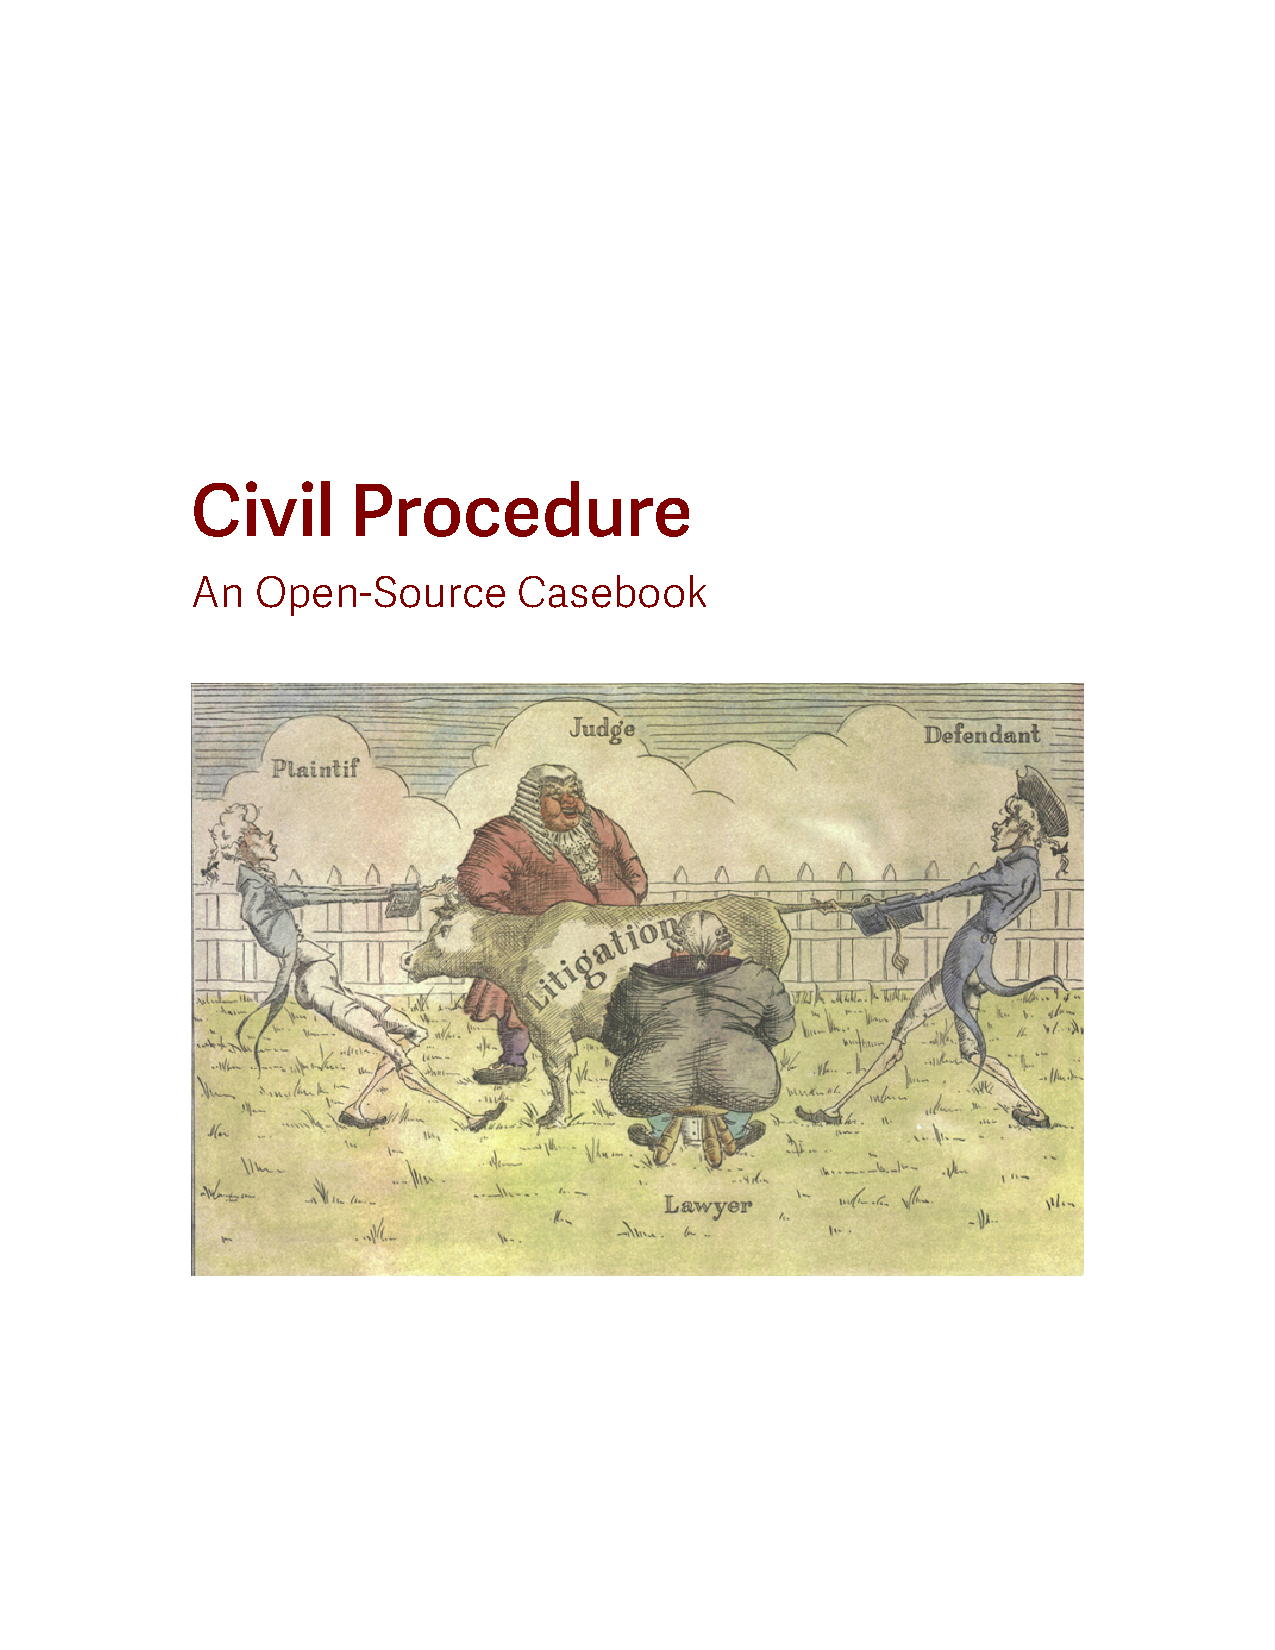
\includepdf{bookcover.pdf}\clearpage}{}

\blankpage

\frontmatter

% Frontispiece
\thispagestyle{empty}

\begin{figure}
\centering
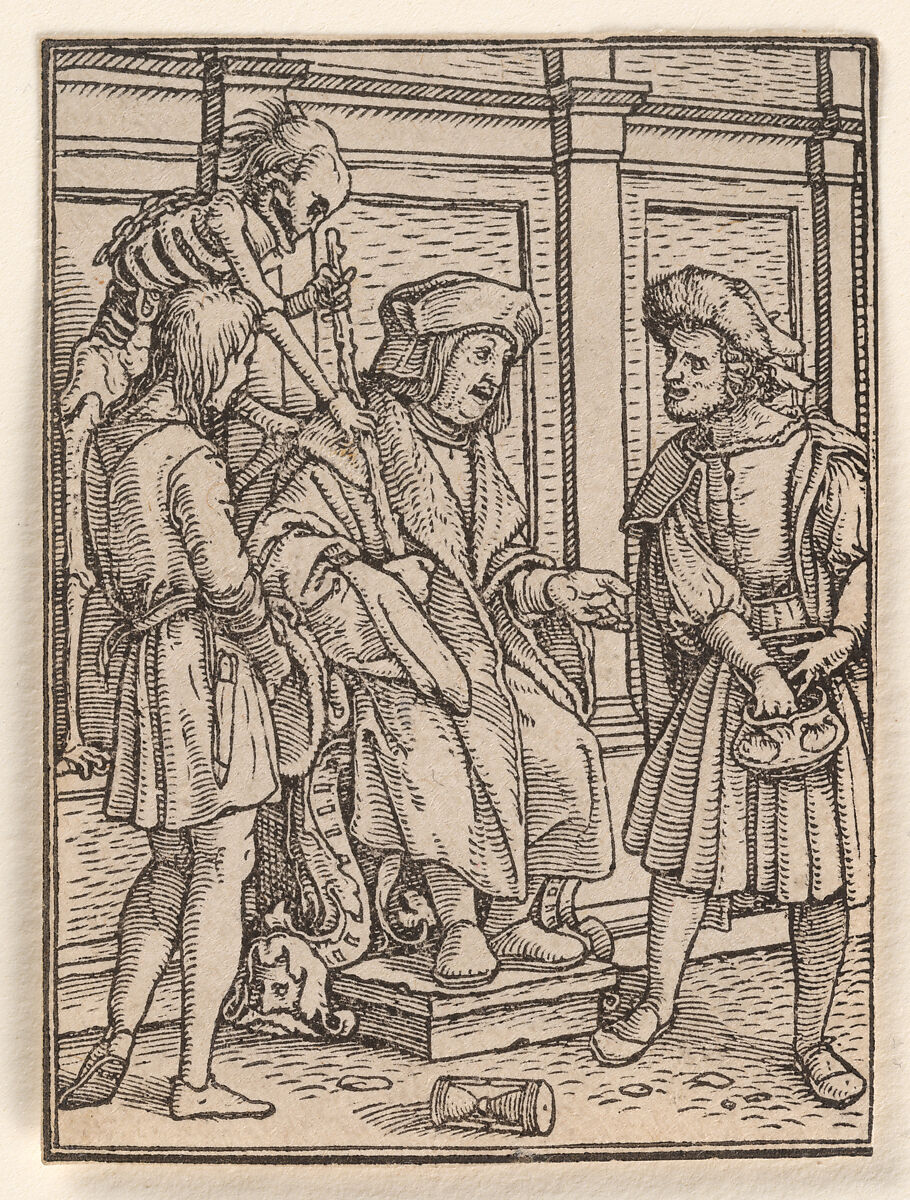
\includegraphics[width=1\textwidth]{../img/frontispiece.jpg}
\end{figure}

\clearpage

% Title page

\thispagestyle{empty}

\begin{flushright}

\vspace*{50mm}

{\bfseries\Huge{Civil Procedure}} 

{\bfseries\vspace{5mm}}

{\Large{An Open-Source Casebook}} 

\vspace{20mm}

{\normalsize{Eric M. Fink}} 

\vspace*{\fill}

\begin{small}

\rmfamily{Elon Law School}  

\rmfamily{\textit{Greensboro, North Carolina}}  

\rmfamily{\monthyear} 

\end{small}

\end{flushright}

\clearpage

% License 

\thispagestyle{empty}
\begingroup
\parindent 0pt
\vspace*{\fill}

\ccbyncsa

\begin{small}
\raggedright{This work is licensed under a Creative Commons Attribution-NonCommercial-ShareAlike 4.0 International License.} \\
\url{https://creativecommons.org/licenses/by-nc-sa/4.0/}

\vspace{1em}

Eric M. Fink\\
Associate Professor of Law \\
Elon University School of Law \\
Greensboro, North Carolina 27408 \\
\url{https://www.emfink.net/ElonLaw/}

\vspace{1em}

Source code: \url{https://github.com/EricMFink/CivProCasebook}

\itshape{version 4.1, \monthyear}

\end{small}
\endgroup

\clearpage

% Epigraph 

\thispagestyle{empty}

\topskip0pt
\vspace*{\fill}
\openepigraph{Jarndyce and Jarndyce drones on. This scarecrow of a suit
has, in course of time, become so complicated that no man alive knows
what it means. The parties to it understand it least, but it has been
observed that no two Chancery lawyers can talk about it for five minutes
without coming to a total disagreement as to all the premises.
Innumerable children have been born into the cause; innumerable young
people have married into it; innumerable old people have died out of it.
Scores of persons have deliriously found themselves made parties in
Jarndyce and Jarndyce without knowing how or why; whole families have
inherited legendary hatreds with the suit. The little plaintiff or
defendant who was promised a new rocking-horse when Jarndyce and
Jarndyce should be settled has grown up, possessed himself of a real
horse, and trotted away into the other world. Fair wards of court have
faded into mothers and grandmothers; a long procession of Chancellors
has come in and gone out; the legion of bills in the suit have been
transformed into mere bills of mortality; there are not three Jarndyces
left upon the earth perhaps since old Tom Jarndyce in despair blew his
brains out at a coffee-house in Chancery Lane; but Jarndyce and Jarndyce
still drags its dreary length before the court, perennially
hopeless.}{Charles Dickens}{Bleak House}
\vspace*{\fill}

% Preface 
\chapter*{Preface}

This casebook presents material for use in a law school Professional Responsibility course. Topics covered include the organization and regulation of the legal profession, the nature of the attorney-client relationship, and the duties that attorneys owe to clients and others.

Most of the materials reproduced here are in the public domain; excerpts from copyrighted materials are included for teaching purposes under the fair use doctrine. Materials have been redacted to omit passages not pertinent to the learning objectives. Judicial opinions have also been "cleaned up" for ease of reading.\footnote{\textit{See} Jack Metzler, {\textit{Cleaning Up Quotations}}, 18 J. App. Prac. \& Process 143 (2017) (proposing "cleaned up" parenthetical for quotations from judicial opinions, to indicate the author “has removed extraneous, non-substantive material like brackets, quotation marks, ellipses, footnote reference numbers, and internal citations; may have changed capitalization without using brackets to indicate that change; and affirmatively represents that the alterations were made solely to enhance readability and that the quotation otherwise faithfully reproduces the quoted text.”)} 
\renewcommand*\contentsname{Contents}
{
\hypersetup{linkcolor=}
\setcounter{tocdepth}{1}
\tableofcontents
}

\mainmatter
\chapter{Foundations of Civil
Procedure}\label{foundations-of-civil-procedure}

\section{At the Threshold}\label{at-the-threshold}

\subsection{\texorpdfstring{Franz Kafka, \emph{Before the Law}
(1915)}{Franz Kafka, Before the Law (1915)}}\label{franz-kafka-before-the-law-1915}

Before the law sits a gatekeeper. To this gatekeeper comes a man from
the country who asks to gain entry into the law. But the gatekeeper says
that he cannot grant him entry at the moment. The man thinks about it
and then asks if he will be allowed to come in later on. ``It is
possible,'' says the gatekeeper, ``but not now.'' At the moment the gate
to the law stands open, as always, and the gatekeeper walks to the side,
so the man bends over in order to see through the gate into the inside.
When the gatekeeper notices that, he laughs and says: ``If it tempts you
so much, try it in spite of my prohibition. But take note: I am
powerful. And I am only the most lowly gatekeeper. But from room to room
stand gatekeepers, each more powerful than the other. I can't endure
even one glimpse of the third.'' The man from the country has not
expected such difficulties: the law should always be accessible for
everyone, he thinks, but as he now looks more closely at the gatekeeper
in his fur coat, at his large pointed nose and his long, thin, black
Tartar's beard, he decides that it would be better to wait until he gets
permission to go inside. The gatekeeper gives him a stool and allows him
to sit down at the side in front of the gate. There he sits for days and
years. He makes many attempts to be let in, and he wears the gatekeeper
out with his requests. The gatekeeper often interrogates him briefly,
questioning him about his homeland and many other things, but they are
indifferent questions, the kind great men put, and at the end he always
tells him once more that he cannot let him inside yet. The man, who has
equipped himself with many things for his journey, spends everything, no
matter how valuable, to win over the gatekeeper. The latter takes it all
but, as he does so, says, ``I am taking this only so that you do not
think you have failed to do anything.'' During the many years the man
observes the gatekeeper almost continuously. He forgets the other
gatekeepers, and this one seems to him the only obstacle for entry into
the law. He curses the unlucky circumstance, in the first years
thoughtlessly and out loud, later, as he grows old, he still mumbles to
himself. He becomes childish and, since in the long years studying the
gatekeeper he has come to know the fleas in his fur collar, he even asks
the fleas to help him persuade the gatekeeper. Finally his eyesight
grows weak, and he does not know whether things are really darker around
him or whether his eyes are merely deceiving him. But he recognizes now
in the darkness an illumination which breaks inextinguishably out of the
gateway to the law. Now he no longer has much time to live. Before his
death he gathers in his head all his experiences of the entire time up
into one question which he has not yet put to the gatekeeper. He waves
to him, since he can no longer lift up his stiffening body.

\begin{figure}[H]

{\centering 
\includegraphics[width=0.33\linewidth,height=\textheight,keepaspectratio]{../img/Mann_zwischen_Gittern.png}

}

\caption{Franz Kafka, Mann zwishen Gittern}

\end{figure}%

\subsection{\texorpdfstring{William Felstiner, et al, \emph{The
Emergence \& Transformation of Disputes}
(1980)}{William Felstiner, et al, The Emergence \& Transformation of Disputes (1980)}}\label{william-felstiner-et-al-the-emergence-transformation-of-disputes-1980}

\subsubsection{I. Introduction}\label{i.-introduction}

The sociology of law has been dominated by studies of officials and
formal institutions and their work products. This agenda has shaped the
way disputes are understood and portrayed. Institutions reify cases by
reducing them to records; they embody disputes in a concrete form that
can be studied retrospectively by attending to the words used by lay
persons and officials and by examining the economic and legal context in
which cases occur. But disputes are not things: they are social
constructs. Their shapes reflect whatever definition the observer gives
to the concept. Moreover, a significant portion of any dispute exists
only in the minds of the disputants.

\subsubsection{II. Where Disputes Come From and How They
Develop}\label{ii.-where-disputes-come-from-and-how-they-develop}

Assume a population living downwind from a nuclear test site. Some
portion of that population has developed cancer as a result of the
exposure and some has not. Some of those stricken know that they are
sick and some do not. In order for disputes to emerge and remedial
action to be taken, an unperceived injurious experience (unPIE, for
short) must be transformed into a perceived injurious experience (PIE).
The uninformed cancer victims must learn that they are sick. The
transformation perspective directs our attention to the differential
transformation of unPIEs into PIEs. It urges us to examine, in this
case, differences in class, education, work situation, social networks,
etc. between those who become aware of their cancer and those who do
not, as well as attend to the possible manipulation of information by
those responsible for the radiation.

This first transformation---saying to oneself that a particular
experience has been injurious---we call \emph{naming}. Though hard to
study empirically, naming may be the critical transformation; the level
and kind of disputing in a society may turn more on what is initially
perceived as an injury than on any later decision. For instance,
asbestosis only became an acknowledged ``disease'' \emph{and} the basis
of a claim for compensation when shipyard workers stopped taking for
granted that they would have trouble breathing after ten years of
installing insulation and came to view their condition as a problem.

The next step is the transformation of a perceived injurious experience
into a grievance. This occurs when a person attributes an injury to the
fault of another individual or social entity. By including fault within
the definition of grievance, we limit the concept to injuries viewed
both as violations of norms and as remediable. The definition takes the
grievant's perspective: the injured person must feel wronged and believe
that something might be done in response to the injury, however
politically or sociologically improbable such a response might be. A
grievance must be distinguished from a complaint against no one in
particular (about the weather, or perhaps inflation) and from a mere
wish unaccompanied by a sense of injury for which another is held
responsible (I might like to be more attractive). We call the
transformation from perceived injurious experience to grievance
\emph{blaming}: our diseased shipyard worker makes this transformation
when he holds his employer or the manufacturer of asbestos insulation
responsible for his asbestosis.

The third transformation occurs when someone with a grievance voices it
to the person or entity believed to be responsible and asks for some
remedy. We call this communication \emph{claiming}. A claim is
transformed into a dispute when it is rejected in whole or in part.
Rejection need not be expressed by words. Delay that the claimant
construes as resistance is just as much a rejection as is a compromise
offer (partial rejection) or an outright refusal.

We know that only a small fraction of injurious experiences ever mature
into disputes. Furthermore, we know that most of the attrition occurs at
the early stages: experiences are not perceived as injurious;
perceptions do not ripen into grievances; grievances are voiced to
intimates but not to the person deemed responsible.

The early stages of naming, blaming, and claiming are significant, not
only because of the high attrition they reflect, but also because the
range of behavior they encompass is greater than that involved in the
later stages of disputes, where institutional patterns restrict the
options open to disputants. Examination of this behavior will help us
identify the social structure of disputing. Transformations reflect
social structural variables, as well as personality traits. People
do---or do not---perceive an experience as an injury, blame someone
else, claim redress, or get their claims accepted because of their
\emph{social position} as well as their individual characteristics. The
transformation perspective points as much to the study of social
stratification as to the exploration of social psychology.

\subsubsection{III. The Characteristics of
Transformation}\label{iii.-the-characteristics-of-transformation}

PIEs, grievances, and disputes have the following characteristics: they
are subjective, unstable, reactive, complicated, and incomplete. They
are \emph{subjective} in the sense that transformations need not be
accompanied by any observable behavior. A disputant discusses his
problem with a lawyer and consequently reappraises the behavior of the
opposing party. The disputant now believes that his opponent was not
just mistaken but acted in bad faith. The content of the dispute has
been transformed in the mind of the disputant, although neither the
lawyer nor the opposing party necessarily knows about the shift.

Since transformations may be nothing more than changes in feelings, and
feelings may change repeatedly, the process is \emph{unstable}. This
characteristic is notable only because it differs so markedly from the
conventional understanding of legal controversies. In the conventional
view of disputes, the sources of claims and rejections are objective
events that happened in the past. It is accepted that it may be
difficult to get the facts straight, but there is rarely an awareness
that the events themselves may be transformed as they are processed.
This view is psychologically naive: it is insensitive to the effect of
feelings on the attribution of motive and to the consequences of such
attributions for the subject's understanding of behavior.

Even in ordinary understanding, disputing is a \emph{complicated}
process involving ambiguous behavior, faulty recall, uncertain norms,
conflicting objectives, inconsistent values, and complex institutions.
It is complicated still further by attention to changes in disputant
feelings and objectives over time. Take the stereotypical case of
personal injury arising out of an automobile accident. A conventional
analysis (e.g., the one often borrowed from economics) assumes that the
goals of the defendant driver are to minimize his responsibility and
limit the complainant's recovery. A transformation view, on the other
hand, suggests that the defendant's objectives may be both less clear
and less stable. Depending on his insurance position, his own
experience, his empathy for, relationship to, and interaction with the
injured person, and the tenor of discussions he may have with others
about the accident and its aftermath, the defendant may at various times
wish to maximize rather than minimize both his own fault and the
complainant's recovery or to take some intermediate position. A
transformation approach would seek to identify these activities and
their effects in order to account for such shifts in objective.

\subsubsection{IV. Subjects and Agents of
Transformation}\label{iv.-subjects-and-agents-of-transformation}

One way to organize the study of the transformations of PIEs,
grievances, and disputes is to identify what is being transformed (the
subjects of transformation) and what does the transforming (the agents
of transformation).

\paragraph{Parties}\label{parties}

Neither the identity nor the number of parties is fixed. New information
about and redefinition of a conflict can lead a party to change his
views about appropriate adversaries or desirable allies. Both may also
be changed by officials of dispute processing agencies. The new parties,
especially if they are groups like the NAACP, ACLU, or Sierra Club, may
adopt a lawsuit as part of a campaign to use the courts as a mechanism
of social change or to mobilize political activity, although social and
political movements may also lose momentum as a collective struggle is
translated into an individual lawsuit. Parties may be dropped as well as
added. A grievance that was originally experienced collectively may be
individualized in the process of becoming a dispute; tort claims as a
response to harm caused by unsafe conditions and disciplinary hearings
as a response to labor disputes are examples.

Obviously, the parties to a conflict are central agents, as well as
objects, in the transformation process. Their behavior will be a
function of personality as it interacts with prior experience and
current pressures. Experience includes involvement in other conflicts;
contact with reference groups, involvement representatives, and
officials; and familiarity with various forms of dispute processing and
remedies. For instance, among the newly enrolled members of a prepaid
legal services plan, those who have previously consulted a lawyer are
more likely to use their membership privileges than are those who have
not. Personality variables that may affect transformations include risk
preferences, contentiousness, and feelings about personal efficacy,
privacy, independence, and attachment to justice (rule-mindedness). Both
experience and personality are in turn related to social structural
variables: class, ethnicity, gender, age.

The relationship between the parties also has significance for
transformations: the sphere of social life that brings them together
(work, residence, politics, recreation)---which may affect the cost of
exit---their relative status, and the history of prior conflict shape
the way in which they will conduct their dispute. In addition, strategic
interaction between the parties in the course of a conflict may have a
major transformational role. An unusual example is the party who seeks
proactively to elicit grievances against himself: the retail seller who
asks purchasers about complaints, the employer who provides an anonymous
suggestion box, even the neurotic spouse or lover who invites
recriminations. But more common are the new elements disputes take on,
the rise and fall in animosity and effort that occurs in response to or
in anticipation of the ``moves'' of the opposition.

\paragraph{Attributions}\label{attributions}

Attribution theory asserts that the causes a person assigns for an
injurious experience will be important determinants of the action he or
she takes in response to it; those attributions will also presumably
affect perception of the experience as injurious. People who blame
themselves for an experience are less likely to see it as injurious, or,
having so perceived it, to voice a grievance about it; they are more
likely to do both if blame can be placed upon another, particularly when
the responsible agent can be seen as intentionally causing or
aggravating the problem. But attributions themselves are not fixed. As
moral coloration is modified by new information, logic, insight, or
experience, attributions are changed, and they alter the participants'
understanding of their experience. Adversary response may be an
important factor in this transformation, as may the nature of the
dispute process. Some processes, such as counseling, may drain the
dispute of moral content and for problems; others, like direct diffuse
responsibility confrontation or litigation, may intensify the
disputant's moral judgment and focus blame. Thus the degree and quality
of blame, an important subject of transformations, also produces further
transformations.

\paragraph{Scope}\label{scope}

The scope of conflict---the extent of relevant discourse about
grievances and claims---is affected both by the objectives and by the
processual and behavior of disputants characteristics of dispute
institutions. A hypothetical case frequently used in mediator training
involves a man's wife and his lover. The wife has hit the lover with a
rock, and the latter has complained to the police; at arraignment the
judge has referred the women to mediation. The discussion there focuses
initially on the rock incident and then expands to include the battle
for the man's affections. The scope of this dispute is thus complicated
by the confrontation between the women during the rock incident,
narrowed to that incident alone as the dispute is handled by police and
court, and then broadened to re-embrace the original conflict plus the
rock incident through interaction between the disputants and the
mediator. Some types of dispute processing seek to narrow the disputes
with which they deal in order to produce a construction of events that
appears manageable. Others are alive to context and circumstance. They
encourage a full rendering of events and exploration of the strands of
interaction, no matter where they lead. The scope of conflict, in turn,
affects the identity of the participants, the tactics used, and the
outcomes that become feasible.

\paragraph{Choice of Mechanisms}\label{choice-of-mechanisms}

The grievant's choice of an audience to whom to voice a complaint and
the disputant's choice of an institution to which to take a controversy
are primarily functions of the person's objectives and will change as
objectives change. Mechanisms may also be determined by exogenous
factors such as the whims of court clerks and lawyers who prefer not to
try cases or who cool out consumers in order to maintain good relations
with retailers. Once a mechanism---court, administrative agency,
mediator, arbitrator, or psychotherapist---is set in motion, it
determines the rules of relevance, cast of actors, costs, delays, norms,
and remedies.

\paragraph{Objectives Sought}\label{objectives-sought}

A party may change his objectives in two ways: what he seeks or is
willing to concede and how much. Stakes go up or down as new information
becomes available, a party's needs change, rules are adjusted, and costs
are incurred. Delay, frustration, and despair may produce a change in
objectives: victims of job discrimination frequently want the job (or
promotion) or nothing at the outset but later become willing to settle
for money. As Aubert noted, the relationship between objectives and
mechanisms is reciprocal: not only do objectives influence the choice of
mechanisms, but mechanisms chosen may alter objectives. Because courts,
for instance, often proceed by using a limited number of norms to
evaluate an even more circumscribed universe of relevant facts, ``the
needs of the parties, their wishes for the future, cease to be relevant
to the solution''. Even where a legal remedy is anticipatory---alimony,
worker's compensation, or tort damages for future loss---the legal
system frequently prefers to award a lump sum rather than order periodic
payments. Finally, the experience of disputing may stimulate a
participant to take steps to avoid similar disputes in the future, or to
structure his behavior so as to place him in a stronger position should
a dispute occur.

\paragraph{Ideology}\label{ideology}

The individual's sense of entitlement to enjoy certain experiences and
be free from others is a function of the prevailing ideology, of which
law is simply a component. The consumer's dissatisfaction with a product
or service may have been influenced by the campaigns of activists, like
Ralph Nader, who assert that consumers have a right to expect high
quality. Legal change may sometimes be a highly effective way of
transforming ideology to create a sense of entitlement. This is the
sense in which, contrary to conventional wisdom, you \emph{can}
legislate morality. Although it would be foolish to maintain that after
\emph{Brown v. Board of Education} every minority child had a sense of
entitlement to integrated education, made a claim against segregation,
and engaged in a dispute when that claim was rejected, surely this has
happened more often \emph{since} than before 1954. Following a recent
television program in Chicago in which a woman subjected to a strip
search during a routine traffic citation described her successful damage
claim against the police department, \emph{hundreds} of women telephoned
the station with similar stories. In this instance, a legal victory
transformed shame into outrage, encouraging the voicing of grievances,
many of which may have become disputes. When the original victim chose a
legal mechanism for her complaint, a collective grievance against police
practices was individualized and depoliticized. When she broadcast her
legal victory on television, the legal dispute was collectivized and
repoliticized. Ideology---and law---can also instill a sense of
disentitlement. The enactment of worker's compensation as the
``solution'' to the problem of industrial accidents early in this
century may have helped convince workers to rely on employer paternalism
to ensure their safety and relinquish claims to control the workplace.

\paragraph{Reference Groups}\label{reference-groups}

Disputes may be transformed through interaction with audiences or
sponsors. A tenant's dispute with a landlord may be the cause around
which a tenants' association is formed; a worker's grievance against a
foreman may become the stimulus to a union organizing drive or a
rank-and-file movement within an existing union. This transformation may
not only make an individual dispute into a collective one: it also may
lead to economic or political struggle displacing legal procedures. This
is especially important in the remedy-seeking behavior of disadvantaged
groups. The movement from law to politics, and the accompanying
expansion of the scope of disputing, are prompted and guided by the
reaction of a wide social network to individual instances of injustice.
Absent the support of such a network, no such movement is likely to
occur. Whether that support is provided depends on a number of
independent variables: the subculture of the audience---which will
define the experience as injurious or harmless, encourage or discourage
the expression of the grievance, and prefer certain dispute processing
strategies; and the social composition of the audience---whether it is
made up of peers or superiors. These variables, in turn, are influenced
by social structural factors---for instance, whether the network in
which the individual is situated is open or closed. In an open network,
where ego is related (separately) to the members but they are not
related to each other, the audience is likely to respond individually,
often seeking to resolve the dispute through the exercise of
superordinate influence. In a closed network, where everybody is related
to everybody, the likelihood of a collective response is much greater.

\paragraph{Representatives and
Officials}\label{representatives-and-officials}

Lawyers, psychotherapists, union officials, social workers, government
functionaries, and other agents and public officials help people
understand their grievances and what they can do about them. In
rendering this service, they almost always produce a transformation: the
essence of professional jobs is \emph{to define the needs of the
consumer} of professional services. Generally, this leads to a
definition that calls for the professional to provide such services.

Of all of the agents of dispute transformation lawyers are probably the
most important. This is, in part, the result of the lawyer's central
role as gatekeeper to legal institutions and facilitator of a wide range
of personal and economic transactions in American society. It is obvious
that lawyers play a central role in dispute decisions. Yet relatively
few studies of lawyer behavior have been informed, even implicitly, by a
transformation perspective. We know more about the structure of the bar
and about particular ethical problems in the practice of law than we do
about how lawyers interact with clients and what difference it makes.

Critics of professionals argue that they ``create'' at least some of the
needs they satisfy. Lawyers exercise considerable power over their
clients. They maintain control over the course of litigation and
discourage clients from seeking a second opinion or taking their
business elsewhere. There is evidence that lawyers often shape disputes
to fit their own interests rather than those of their clients. Sometimes
they systematically ``cool out'' clients with legitimate grievances. In
consumer cases lawyers may be reluctant to press claims for fear of
press offending potential business clients. In defending the accused
criminal, lawyers may prefer negotiating a plea bargain to trying the
case. In tort litigation they prefer to settle, and may offer package
deals to claims adjusters. In other cases they may amplify grievances:
some divorce lawyers recommend litigation for which a substantial fee
can be charged, rather than engage in difficult, problematic, and
unprofitable negotiations about reconciliation.

Lawyers may affect transformations in another way---by rejecting
requests for assistance or providing only minimal help and thereby
arresting the further development of a dispute, at least through legal
channels. Limited data suggest that lawyers respond differently to
different categories of clients. This differential lawyer response
contributes to variation in dispute behavior between poor and middle
class, corporate entities and individuals, normal and deviant, members
of ethnic majorities and minorities, and young and old.

Of course, lawyers also produce transformations about which we may be
more enthusiastic. They furnish information about choices and
consequences unknown to clients; offer a forum for testing the reality
of the client's perspective; help clients identify, explore, organize,
and negotiate their problems; and give emotional and social support to
clients who are unsure of themselves or their objectives.

Enforcement personnel---police, prosecutors, regulatory agencies---may
also produce transformations: seeking disputes in order to advance a
public policy or generate a caseload that will justify increased budget
demands; discouraging disputes because of personnel shortages; or
selectively encouraging those disputes that enhance the prestige of the
agency and discouraging those that diminish its significance or call for
skills it lacks or are thought to be inappropriate.

\paragraph{Dispute Institutions}\label{dispute-institutions}

Courts, which fall at one extreme along most of the dimensions useful
for describing dispute institutions, may transform the content of
disputes because the substantive norms they apply differ from rules of
custom or ordinary morality, and their unique norms may narrow issues
and circumscribe procedural evidence.

Courts may transform disputes by individualizing remedies. Some of the
victims of a defective product may want to force the manufacturer to
alter the production process. But because courts award only money
damages for unintentional torts, even those victims' concept of an
acceptable outcome is transformed from a collective good (safety) into
individual enrichment, a transformation greatly encouraged by the
lawyer's interest in creating a fund out of which his fee can be paid.

Because of the monopoly exercised by lawyers, the esoteric nature of
court processes and discourse, and the burdens of pretrial procedure,
the \emph{attitude} of disputants may be altered by their minimal role
in the courtroom and the way they are treated there. In effect, their
``property'' interest in the dispute is expropriated by lawyers and the
state. The rediscovery of the victim in the criminal prosecution is one
recognition of this. Furthermore, delays caused by court overload or
foot-dragging by an adversary may transform what disputants would
otherwise consider a useful procedure into pointless frustration.

The nature and potential transformational effects of courts can be seen
best if we contrast litigation with another technique for handling
conflict---psychotherapy. Like law, therapy individualizes conflicts and
remedies. In most other ways, however, it sharply contrasts with courts
and lawyers. Disputants are encouraged to describe the conflict and
express their feelings about it in whatever terms they find comfortable.
Since mental health professionals are trained to use anger to reduce
hostility, disputants will not need to deny their feelings. The
nonjudgmental posture and reflective responses of the therapist should
provide emotional support for disputants, who are urged to examine the
pattern of their own responses to the behavior of others. They may find,
for instance, that progress toward a solution may be obstructed not by
the dilatory tactics or opposition of an adversary but rather by their
own reluctance to act. One objective of the process is to increase the
disputant's understanding of the motives, feelings, and behavior of
others. Thus, where the outcome of successful litigation is usually an
order directed to an adversary, the outcome of a successful
psychotherapeutic intervention may be a change in the client.

In between courts and psychotherapy there are many other dispute
institutions---arbitration, mediation, administrative hearings, and
investigations---that use ingredients of each process in different
combinations but always effect a transformation.

\section{Civil Litigation in Federal
Court}\label{civil-litigation-in-federal-court}

\subsection{U.S. Constitution, Article
III}\label{u.s.-constitution-article-iii}

\subsubsection{Section 1}\label{section-1}

The judicial power of the United States, shall be vested in one Supreme
Court, and in such inferior courts as the Congress may from time to time
ordain and establish. The judges, both of the supreme and inferior
courts, shall hold their offices during good behaviour, and shall, at
stated times, receive for their services, a compensation, which shall
not be diminished during their continuance in office.

\subsubsection{Section 2}\label{section-2}

The judicial power shall extend to all cases, in law and equity, arising
under this Constitution, the laws of the United States, and treaties
made, or which shall be made, under their authority;--to all cases
affecting ambassadors, other public ministers and consuls;--to all cases
of admiralty and maritime jurisdiction;--to controversies to which the
United States shall be a party;--to controversies between two or more
states;--between a state and citizens of another state;--between
citizens of different states;--between citizens of the same state
claiming lands under grants of different states, and between a state, or
the citizens thereof, and foreign states, citizens or subjects.

In all cases affecting ambassadors, other public ministers and consuls,
and those in which a state shall be party, the Supreme Court shall have
original jurisdiction. In all the other cases before mentioned, the
Supreme Court shall have appellate jurisdiction, both as to law and
fact, with such exceptions, and under such regulations as the Congress
shall make.

\subsection{\texorpdfstring{Administrative Office of the U.S. Courts,
\emph{Understanding the Federal
Courts}}{Administrative Office of the U.S. Courts, Understanding the Federal Courts}}\label{administrative-office-of-the-u.s.-courts-understanding-the-federal-courts}

\subsubsection{Structure of the Federal
Courts}\label{structure-of-the-federal-courts}

The Supreme Court is the highest court in the United States. Article III
of the U.S. Constitution created the Supreme Court and authorized
Congress to pass laws establishing a system of lower courts. In the
federal court system's present form, 94 district-level trial courts and
13 courts of appeals sit below the Supreme Court.

\paragraph{Trial Courts}\label{trial-courts}

The U.S. district courts are the primary trial courts of the federal
court system. Within limits set by Congress and the Constitution, the
district courts have jurisdiction to hear nearly all categories of
federal cases, including both civil and criminal matters. There are 94
federal judicial districts, including at least one district in each
state, the District of Columbia, and Puerto Rico. Each district includes
a U.S. bankruptcy court as a unit of the district court.

There are two special trial courts that have nationwide jurisdiction
over certain types of cases. The Court of International Trade addresses
cases involving international trade and customs issues. The United
States Court of Federal Claims has jurisdiction over most claims for
money damages against the United States, disputes over federal
contracts, unlawful ``takings'' of private property by the federal
government, vaccine injury cases, and a variety of other claims against
the United States.

Three territories of the United States--- the Virgin Islands, Guam, and
the Northern Mariana Islands---have U.S. district courts that hear
federal cases, including bankruptcy cases.

\begin{figure}[H]

{\centering 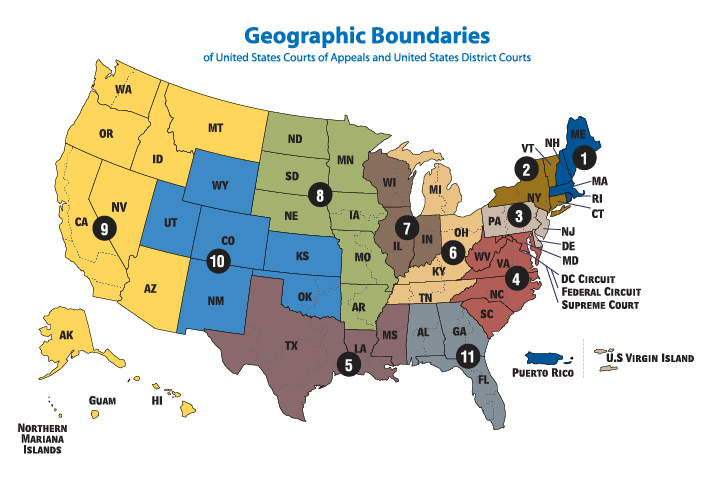
\includegraphics[width=0.33\linewidth,height=\textheight,keepaspectratio]{../img/FedCourtsMap.png}

}

\caption{Federal District Courts \& Appellate Circuits}

\end{figure}%

\paragraph{Appellate Courts}\label{appellate-courts}

The 94 judicial districts are organized into 12 regional circuits, each
of which has a United States court of appeals. A court of appeals hears
challenges to district court decisions from courts located within its
circuit, as well as appeals from decisions of federal administrative
agencies. In addition, the Court of Appeals for the Federal Circuit has
nationwide jurisdiction to hear appeals in specialized cases, such as
those involving patent laws and cases decided by the Court of
International Trade and the Court of Federal Claims.

\paragraph{United States Supreme
Court}\label{united-states-supreme-court}

The U.S. Supreme Court consists of the Chief Justice of the United
States and eight associate justices. At its discretion, and within
certain guidelines established by Congress, the Supreme Court hears a
small percentage of the cases it is asked to decide each year. Supreme
Court cases are usually selected either because the lower courts have
differed, or ``split,'' on a legal issue or they involve important
questions about the Constitution or federal law.

\subsubsection{Jurisdiction of the Federal
Courts}\label{jurisdiction-of-the-federal-courts}

Before a federal court can hear a case, or ``exercise its
jurisdiction,'' certain conditions must be met.

First, under the Constitution, federal courts exercise only ``judicial''
powers. This means that federal judges may interpret the law only
through the resolution of actual legal disputes, referred to in Article
III of the Constitution as ``Cases or Controversies.'' A court cannot
attempt to correct a problem on its own initiative, or to answer a
hypothetical legal question.

Second, in an actual case or controversy, the plaintiff in a federal
lawsuit also must have legal ``standing'' to ask the court for a
decision. That means the plaintiff must have been aggrieved, or legally
harmed in some way, by the defendant.

Third, the case must present a category of dispute that the law in
question was designed to address, and it must be a complaint that the
court has the power to remedy. In other words, the court must be
authorized, under the Constitution or a federal law, to hear the case
and grant appropriate relief to the plaintiff.

Finally, the case cannot be ``moot,'' that is, it must present an
ongoing problem for the court to resolve. The federal courts, thus, are
courts of ``limited'' jurisdiction because they may only decide certain
types of cases as provided by Congress or as identified in the
Constitution.

Although the details of the complex web of federal jurisdiction that
Congress has given the federal courts is beyond the scope of this brief
guide,{\marginnote{\begin{footnotesize}Federal subject matter
jurisdiction is covered in Chapter 3\end{footnotesize}}} it is important
to understand that there are two main sources of the cases coming before
the federal courts: ``federal question'' jurisdiction and ``diversity''
jurisdiction.

In general, federal question jurisdiction arises in cases that involve
the U.S. government, the U.S. Constitution or federal laws, or
controversies between states or between the United States and foreign
governments. A case that raises such a ``federal question'' may be filed
in federal court. Examples of such cases might include a claim by an
individual for entitlement to money under a federal government program
such as Social Security, a criminal prosecution by the government that
alleges someone violated a federal law, or a challenge to actions taken
by a federal agency.

A case also may be filed in federal court based on the ``diversity of
citizenship'' of the litigants, such as between citizens of different
states, or between U.S. citizens and those of another country. To ensure
fairness to the out-of-state litigant, the Constitution provides that
such cases may be heard in a federal court. An important limit to
diversity jurisdiction is that only cases involving more than \$75,000
in potential damages may be filed in a federal court. Claims below that
amount may only be pursued in state court. Moreover, any diversity
jurisdiction case regardless of the amount of money involved may be
brought in a state court rather than a federal court.

Federal courts also have jurisdiction over all bankruptcy matters, which
Congress has determined should be addressed in federal courts rather
than the state courts. Through the bankruptcy process, individuals or
businesses that can no longer pay their creditors may either seek a
court-supervised liquidation of their assets, or they may reorganize
their financial affairs and work out a plan to pay their debts.

Although federal courts are located in every state, they are not the
only forum available to potential litigants. In fact, the great majority
of legal disputes in American courts, civil or criminal, are addressed
in the separate state court systems. State courts have jurisdiction over
virtually all divorce and child custody matters, probate and inheritance
issues, real estate questions, and juvenile matters, and they handle
most criminal cases, contract disputes, traffic violations, and personal
injury cases. In addition, certain categories of legal disputes may be
resolved in special courts or entities that are part of the federal
executive or legislative branches or state and federal administrative
agencies.

\subsection{The Rules Enabling Act, 28 U.S.C. §2071 et
seq.}\label{the-rules-enabling-act-28-u.s.c.-2071-et-seq.}

\subsubsection{§2071--Rule-making power
generally}\label{rule-making-power-generally}

(a) The Supreme Court and all courts established by Act of Congress may
from time to time prescribe rules for the conduct of their business.
Such rules shall be consistent with Acts of Congress and rules of
practice and procedure prescribed under section 2072 of this title.

(b) Any rule prescribed by a court, other than the Supreme Court, under
subsection (a) shall be prescribed only after giving appropriate public
notice and an opportunity for comment. Such rule shall take effect upon
the date specified by the prescribing court and shall have such effect
on pending proceedings as the prescribing court may order.

(c)

\begin{itemize}
\item
  (1) A rule of a district court prescribed under subsection (a) shall
  remain in effect unless modified or abrogated by the judicial council
  of the relevant circuit.
\item
  (2) Any other rule prescribed by a court other than the Supreme Court
  under subsection (a) shall remain in effect unless modified or
  abrogated by the Judicial Conference.
\end{itemize}

(d) Copies of rules prescribed under subsection (a) by a district court
shall be furnished to the judicial council, and copies of all rules
prescribed by a court other than the Supreme Court under subsection (a)
shall be furnished to the Director of the Administrative Office of the
United States Courts and made available to the public.

(e) If the prescribing court determines that there is an immediate need
for a rule, such court may proceed under this section without public
notice and opportunity for comment, but such court shall promptly
thereafter afford such notice and opportunity for comment.

(f) No rule may be prescribed by a district court other than under this
section.

\subsubsection{§2072--Rules of procedure and evidence; power to
prescribe}\label{rules-of-procedure-and-evidence-power-to-prescribe}

(a) The Supreme Court shall have the power to prescribe general rules of
practice and procedure and rules of evidence for cases in the United
States district courts (including proceedings before magistrate judges
thereof) and courts of appeals.

(b) Such rules shall not abridge, enlarge or modify any substantive
right. All laws in conflict with such rules shall be of no further force
or effect after such rules have taken effect.

(c) Such rules may define when a ruling of a district court is final for
the purposes of appeal under section 1291 of this title.

\subsubsection{§2073--Rules of procedure and evidence; method of
prescribing}\label{rules-of-procedure-and-evidence-method-of-prescribing}

(a)

\begin{itemize}
\item
  (1) The Judicial Conference shall prescribe and publish the procedures
  for the consideration of proposed rules under this section.
\item
  (2) The Judicial Conference may authorize the appointment of
  committees to assist the Conference by recommending rules to be
  prescribed under sections 2072 and 2075 of this title. Each such
  committee shall consist of members of the bench and the professional
  bar, and trial and appellate judges.
\end{itemize}

(b) The Judicial Conference shall authorize the appointment of a
standing committee on rules of practice, procedure, and evidence under
subsection (a) of this section. Such standing committee shall review
each recommendation of any other committees so appointed and recommend
to the Judicial Conference rules of practice, procedure, and evidence
and such changes in rules proposed by a committee appointed under
subsection (a)(2) of this section as may be necessary to maintain
consistency and otherwise promote the interest of justice.

(c)

\begin{itemize}
\item
  (1) Each meeting for the transaction of business under this chapter by
  any committee appointed under this section shall be open to the
  public, except when the committee so meeting, in open session and with
  a majority present, determines that it is in the public interest that
  all or part of the remainder of the meeting on that day shall be
  closed to the public, and states the reason for so closing the
  meeting. Minutes of each meeting for the transaction of business under
  this chapter shall be maintained by the committee and made available
  to the public, except that any portion of such minutes, relating to a
  closed meeting and made available to the public, may contain such
  deletions as may be necessary to avoid frustrating the purposes of
  closing the meeting.
\item
  (2) Any meeting for the transaction of business under this chapter, by
  a committee appointed under this section, shall be preceded by
  sufficient notice to enable all interested persons to attend.
\end{itemize}

(d) In making a recommendation under this section or under section 2072
or 2075, the body making that recommendation shall provide a proposed
rule, an explanatory note on the rule, and a written report explaining
the body's action, including any minority or other separate views.

(e) Failure to comply with this section does not invalidate a rule
prescribed under section 2072 or 2075 of this title.

\subsubsection{§2074--Rules of procedure and evidence; submission to
Congress}\label{rules-of-procedure-and-evidence-submission-to-congress}

(a) The Supreme Court shall transmit to the Congress not later than May
1 of the year in which a rule prescribed under section 2072 is to become
effective a copy of the proposed rule. Such rule shall take effect no
earlier than December 1 of the year in which such rule is so transmitted
unless otherwise provided by law. The Supreme Court may fix the extent
such rule shall apply to proceedings then pending, except that the
Supreme Court shall not require the application of such rule to further
proceedings then pending to the extent that, in the opinion of the court
in which such proceedings are pending, the application of such rule in
such proceedings would not be feasible or would work injustice, in which
event the former rule applies.

(b) Any such rule creating, abolishing, or modifying an evidentiary
privilege shall have no force or effect unless approved by Act of
Congress.

\subsection{Fed. R. Civ. P. Rule 1}\label{fed.-r.-civ.-p.-rule-1}

\subsubsection{Scope and Purpose}\label{scope-and-purpose}

These rules govern the procedure in all civil actions and proceedings in
the United States district courts, except as stated in Rule 81. They
should be construed, administered, and employed by the court and the
parties to secure the just, speedy, and inexpensive determination of
every action and proceeding.

\subsection{Fed. R. Civ. P. Rule 2}\label{fed.-r.-civ.-p.-rule-2}

\subsubsection{One Form of Action}\label{one-form-of-action}

There is one form of action---the civil action.

\subsection{Stages of a Civil Suit}\label{stages-of-a-civil-suit}

Before commencing a suit, a lawyer (in consultation with the client)
must decide who will be named as parties (Party Joinder), what claims to
assert (Claim Joinder), and where to file the suit (Subject Matter
Jurisdiction, Personal Jurisdiction, \& Venue). Decisions about joinder
may constrain the choice of forum, and vice versa. The limited subject
matter jurisdiction of the federal courts means that federal courts may
only decide certain claims. The constitutional limits on personal
jurisdiction mean that courts may only decide cases against defendants
having sufficient contacts with the forum state. At some point, it may
also be necessary to determine which law---state or federal, and if
state law, which state---will apply to the various issues in the case.

\begin{figure}[H]

{\centering 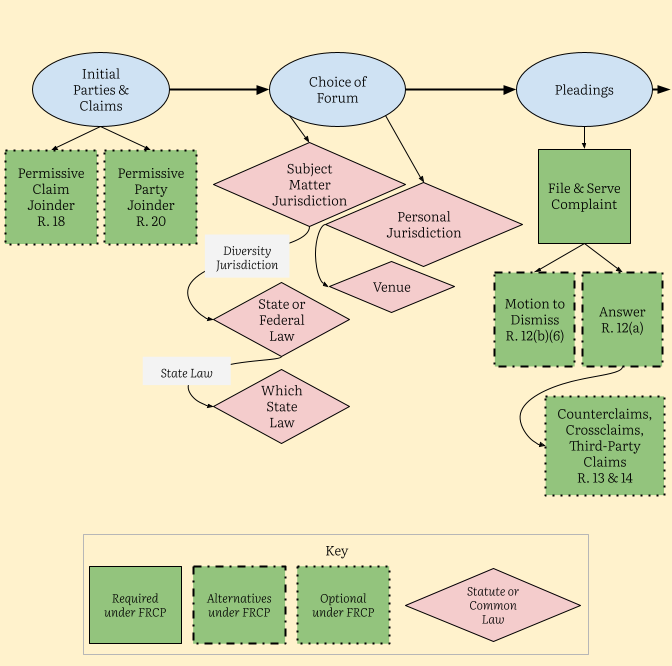
\includegraphics[width=0.6\linewidth,height=\textheight,keepaspectratio]{../img/CivilAction1.png}

}

\caption{Stages of a Civil Suit, part 1}

\end{figure}%

The next step is to file a complaint with the court and serve a copy on
the defendant. The defendant must then respond, either by admitting or
denying the allegations in the complaint (Answer) or moving to dismiss
on procedural grounds (Rule 12 Motions). Defendants may also assert
claims of their own against the plaintiff, other defendants, or new
parties (Counterclaims, Crossclaims, Third party claims).

If the case is not dismissed at the pleadings stage, the parties will
produce evidence (Discovery). They may also ask the court to decide the
suit, or particular issues, based on the evidence in the pre-trial
record (Summary Judgment).

\begin{figure}[H]

{\centering 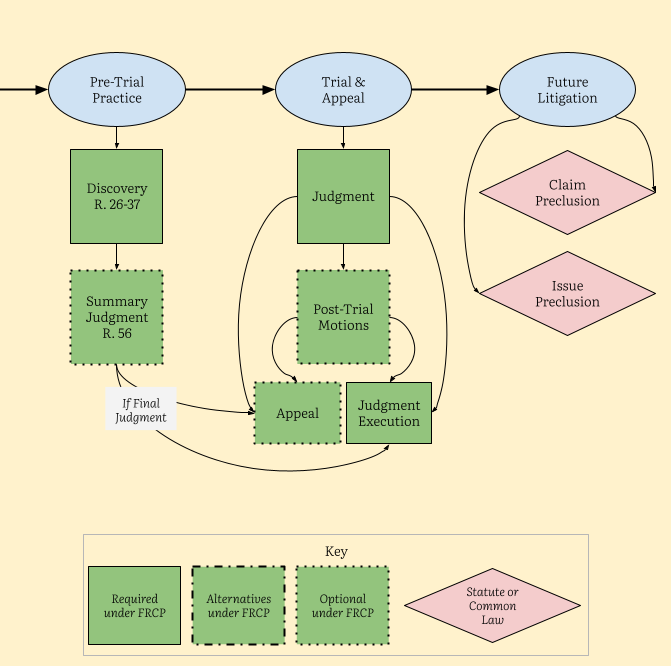
\includegraphics[width=0.6\linewidth,height=\textheight,keepaspectratio]{../img/CivilAction2.png}

}

\caption{Stages of a Civil Suit, part 2}

\end{figure}%

If the case is not fully decided on summary judgment (or settled), it
will proceed to trial, at the end of which the court will enter judgment
in favor of the prevailing party. The losing party may then appeal to a
higher court. A final judgment may have consequences for other lawsuits
involving the same parties (Claim and Issue Preclusion).

\chapter{Parties \& Claims}\label{parties-claims}

\section{Permissive Joinder of
Claims}\label{permissive-joinder-of-claims}

\subsection{Fed. R. Civ. P. Rule 18}\label{fed.-r.-civ.-p.-rule-18}

(a) In General. A party asserting a claim, counterclaim, crossclaim, or
third-party claim may join, as independent or alternative claims, as
many claims as it has against an opposing party.

(b) Joinder of Contingent Claims. A party may join two claims even
though one of them is contingent on the disposition of the other; but
the court may grant relief only in accordance with the parties' relative
substantive rights. In particular, a plaintiff may state a claim for
money and a claim to set aside a conveyance that is fraudulent as to
that plaintiff, without first obtaining a judgment for the money.

\subsection{Fed. R. Civ. P. Rule 42}\label{fed.-r.-civ.-p.-rule-42}

(a) Consolidation. If actions before the court involve a common question
of law or fact, the court may:

\begin{itemize}
\item
  (1) join for hearing or trial any or all matters at issue in the
  actions;
\item
  (2) consolidate the actions; or
\item
  (3) issue any other orders to avoid unnecessary cost or delay.
\end{itemize}

(b) Separate Trials. For convenience, to avoid prejudice, or to expedite
and economize, the court may order a separate trial of one or more
separate issues, claims, crossclaims, counterclaims, or third-party
claims. When ordering a separate trial, the court must preserve any
federal right to a jury trial.

\subsection{Burdine v. Metropolitan Direct Property and Casualty Ins.
Co.~(E.D. Ky.
2018)}\label{burdine-v.-metropolitan-direct-property-and-casualty-ins.-co.-e.d.-ky.-2018}

Plaintiff Paulina Brooke Burdine originally filed this lawsuit against
defendant Metropolitan Direct Property and Casualty Insurance Company
(hereinafter ``MetDirect'') in Franklin Circuit Court. MetDirect removed
the proceedings to this Court pursuant to 28 U.S.C. §1332. Ms.~Burdine
asserts two claims against MetDirect stemming from two separate
automobile accidents. MetDirect moved to sever these claims or, in the
alternative, bifurcate the proceedings. For the following reasons,
MetDirect's Motion to Sever or Bifurcate is DENIED.

Ms.~Burdine initiated this lawsuit in the wake of two separate
automobile accidents. Collision one took place in Scott County, Kentucky
when Sandy Strong ran a red light and struck Ms.~Burdine's vehicle.
Ms.~Strong admitted fault, and her insurance policy paid Ms.~Burdine to
its limits. Collision two took place in Fayette County, Kentucky when
Phillip Smith failed to yield the right of way to Ms.~Burdine and struck
her vehicle. Again, Mr.~Smith admitted fault and his insurance paid
Ms.~Burdine to its limits. \emph{Id.} At all relevant times, Ms.~Burdine
carried Underinsured Motorist Insurance from MetDirect.

On both occasions, the drivers carried only \$25,000 in liability
insurance. Ms.~Burdine alleges that her medical expenses from each
accident exceed the \$25,000 that she received from the other drivers'
insurance policies. Ms.~Burdine now wishes to collect compensation from
MetDirect, her own insurance carrier, because her hospital expenses are
in excess of what she received from the policies of the other drivers.

Joinder of claims is governed by Federal Rule of Civil Procedure 18,
which states ``a party asserting a claim, counterclaim, crossclaim, or
third-party claim may join, as independent or alternative clams, as many
claims as it has against an opposing party.'' The scope of Rule 18(a) is
well settled: ``The claims which may properly be joined under Rule 18(a)
include those which arise out of separate and independent transactions
or occurrences, as well as those which arise out of a single transaction
or occurrence.''

MetDirect argues that Ms.~Burdine's claims against it are improperly
joined in a single action and should be severed. In support of its
position, MetDirect cites Federal Rule of Civil Procedure 20(a)(2),
which governs the joinder of parties. But this is the wrong rule. ``Rule
20 deals solely with joinder of parties and becomes relevant only when
there is more than one party on one or both sides of the action. It is
not concerned with joinder of claims, which is governed by rule 18.''

MetDirect is correct that Ms.~Burdine has asserted two separate claims
involving two separate, negligent drivers. In its motion, MetDirect
tries to analogize this suit to one against two separate, negligent
drivers, and argues that Ms.~Burdine will have to prove their negligence
to recover at trial. But Ms.~Burdine has not sued these drivers in
negligence. Rather, she is suing MetDirect in contract, and whatever
evidence of the drivers' negligence Ms.~Burdine will have to show at
trial, those drivers are not defendants. There is but one defendant in
this action---MetDirect---and Ms.~Burdine has two claims against that
defendant. As such, Ms.~Burdine's claims are properly joined under Rule
18(a). Whether or not Ms.~Burdine could have sued the individual drivers
for negligence in a single action is irrelevant.

While Ms.~Burdine's claims are properly joined against MetDirect under
Rule 18, the Court may sever them if inconvenience would result ``from
trying two matters together which have little or nothing in common.''
However, ``the joinder of claims is strongly encouraged, and,
concomitantly, severance should generally be granted only in
`exceptional circumstances.'\,''

Rule 42 governs the bifurcation of civil trials. \emph{See} Fed. R. Civ.
P. 42(b). It states in relevant part, ``For convenience, to avoid
prejudice, or to expedite and economize, the court may order a separate
trial of one or more separate issues, claims, crossclaims,
counterclaims, or third-party claims.'' ``Bifurcation may be appropriate
`where the evidence offered on two different issues will be wholly
distinct.'\,'' The movant has the burden of proving the appropriateness
of bifurcation.

MetDirect argues that bifurcation is necessary to avoid confusing the
jury. Specifically, MetDirect is concerned that ``the commingling of
Plaintiff's claimed damages will .. . render it difficult, if not
impossible, for the jury to accurately determine the amount of damages
attributable to each incident,'' which would prejudice MetDirect. But
this is a problem that cannot be avoided even with bifurcation.
Ms.~Burdine's collisions occurred approximately ten months apart.
Ms.~Burdine was still rehabilitating injuries from collision one when
she was involved in collision two. At the very least, a jury assessing
damages resulting from collision two will be forced to consider
collision one to try and distinguish what harm is attributable solely to
the second collision.

In fact, the greater risk of prejudice lies with Ms.~Burdine should the
Court sever these claims. To do so would force Ms.~Burdine to
participate in two lawsuits, greatly increasing her costs particularly
with respect to medical expert testimony to her injuries. Likewise, the
Court would be burdened both by the time and expense of separate
proceedings in this instance. Further, as counsel for Ms.~Burdine aptly
puts in the Response to Defendant's Motion to Sever:

\begin{quote}
If two trials are held, then at each trial Defendant could attempt to
blame plaintiff's injuries on the other collision. If such tactic were
successful, there is the possibility that \emph{each} jury could decided
to attribute all of Plaintiff's injures to the other collision and award
Plaintiff nothing when in fact all of Plaintiff's injuries are
attributable to the two collisions.
\end{quote}

Finally, the evidence offered on these two claims would not be ``wholly
inconsistent'' such that bifurcation is necessary. The insurance
companies of the other drivers, Ms.~Strong and Mr.~Smith, have already
paid Ms.~Burdine to the limit of their policies. The larger issue at
trial, then, will not be their negligence, but whether the damages
Ms.~Burdine suffered exceed the \$25,000.00 offered under the other
drivers' respective policies. Therefore, no reason exists to bifurcate
these issues at trial.

In sum, Ms.~Burdine has properly joined her claims, which sound in
contract, against single defendant MetDirect. This issue is controlled
by Federal Rule of Civil Procedure 18, and Rule 20 has no applicability
here. Further, MetDirect will not be prejudiced by trying these claims
together. On the contrary, the risk of prejudice to Ms.~Burdine is high
should her claims be severed, and severance would not convenience,
expedite or economize the proceedings. \emph{See} Fed. R. Civ. P. 42(b).

\section{Permissive Joinder of
Parties}\label{permissive-joinder-of-parties}

\subsection{Fed. R. Civ. P. Rule 20}\label{fed.-r.-civ.-p.-rule-20}

(a) Persons Who May Join or Be Joined.

\begin{itemize}
\item
  (1) Plaintiffs. Persons may join in one action as plaintiffs if:

  \begin{itemize}
  \item
    (A) they assert any right to relief jointly, severally, or in the
    alternative with respect to or arising out of the same transaction,
    occurrence, or series of transactions or occurrences; and
  \item
    (B) any question of law or fact common to all plaintiffs will arise
    in the action.
  \end{itemize}
\item
  (2) Defendants. Persons---as well as a vessel, cargo, or other
  property subject to admiralty process in rem---may be joined in one
  action as defendants if:

  \begin{itemize}
  \item
    (A) any right to relief is asserted against them jointly, severally,
    or in the alternative with respect to or arising out of the same
    transaction, occurrence, or series of transactions or occurrences;
    and
  \item
    (B) any question of law or fact common to all defendants will arise
    in the action.
  \end{itemize}
\item
  (3) Extent of Relief. Neither a plaintiff nor a defendant need be
  interested in obtaining or defending against all the relief demanded.
  The court may grant judgment to one or more plaintiffs according to
  their rights, and against one or more defendants according to their
  liabilities.
\end{itemize}

(b) Protective Measures. The court may issue orders---including an order
for separate trials---to protect a party against embarrassment, delay,
expense, or other prejudice that arises from including a person against
whom the party asserts no claim and who asserts no claim against the
party.

\subsection{Mosley v. General Motors Corp.~(E.D. Missouri
1980)}\label{mosley-v.-general-motors-corp.-e.d.-missouri-1980}

Nathaniel Mosley and nine other persons joined in bringing this action
individually and as class representatives alleging that their rights
guaranteed under 42 U.S.C. §2000e et seq. and 42 U.S.C. §1981 were
denied by General Motors and Local 25, United Automobile, Aerospace and
Agriculture Implement Workers of America Union by reason of their color
and race. Each of the ten named plaintiffs had, prior to the filing of
the complaint, filed a charge with the Equal Employment Opportunity
Commission EEOC asserting the facts underlying these claims. Pursuant
thereto, the EEOC made a reasonable cause finding that General Motors,
Fisher Body Division and Chevrolet Division, and the Union had engaged
in unlawful employment practices in violation of Title VII of the Civil
Rights Act of 1964. Accordingly, the charging parties were notified by
EEOC of their right to institute a civil action in the appropriate
federal district court, pursuant to §706(e) of Title VII, 42 U.S.C.
§2000e-5(e).

In each of the first eight counts of the twelve-count complaint, eight
of the ten plaintiffs alleged that General Motors, Chevrolet Division,
had engaged in unlawful employment practices by: ``discriminating
against Negroes as regards promotions, terms and conditions of
employment''; ``retaliating against Negro employees who protested
actions made unlawful by Title VII of the Act and by discharging some
because they protested said unlawful acts''; ``failing to hire Negro
employees as a class on the basis of race''; ``failing to hire females
as a class on the basis of sex''; ``discharging Negro employees on the
basis of race''; and ``discriminating against Negroes and females in the
granting of relief time.'' Each additionally charged that the defendant
Union had engaged in unlawful employment practices ``with respect to the
granting of relief time to Negro and female employees'' and ``by failing
to pursue 6a grievances.'' The remaining two plaintiffs made similar
allegations against General Motors, Fisher Body Division. All of the
individual plaintiffs requested injunctive relief, back pay, attorneys
fees and costs.

The district court ordered that ``insofar as the first ten counts are
concerned, those ten counts shall be severed into ten separate causes of
action,'' and each plaintiff was directed to bring a separate action
based upon his complaint, duly and separately filed.

In reaching this conclusion on joinder, the district court followed the
reasoning of \emph{Smith v. North American Rockwell Corp.}, which, in a
somewhat analogous situation, found there was no right to relief arising
out of the same transaction, occurrence or series of transactions or
occurrences, and that there was no question of law or fact common to all
plaintiffs sufficient to sustain joinder under Federal Rule of Civil
Procedure 20(a). Similarly, the district court here felt that the
plaintiffs' joint actions against General Motors and the Union presented
a variety of issues having little relationship to one another; that they
had only one common problem, i. e. the defendant; and that as pleaded
the joint actions were completely unmanageable. Upon entering the order,
and upon application of the plaintiffs, the district court found that
its decision involved a controlling question of law as to which there is
a substantial ground for difference of opinion and that any of the
parties might make application for appeal under 28 U.S.C. §1292(b). We
granted the application to permit this interlocutory appeal and for the
following reasons we affirm in part and reverse in part.

Rule 20(a) of the Federal Rules of Civil Procedure provides:

\begin{quote}
All persons may join in one action as plaintiffs if they assert any
right to relief jointly, severally, or in the alternative in respect of
or arising out of the same transaction, occurrence, or series of
transactions or occurrences and if any question of law or fact common to
all these persons will arise in the action.
\end{quote}

Additionally, Rule 20(b) and Rule 42(b) vest in the district court the
discretion to order separate trials or make such other orders as will
prevent delay or prejudice. In this manner, the scope of the civil
action is made a matter for the discretion of the district court, and a
determination on the question of joinder of parties will be reversed on
appeal only upon a showing of abuse of that discretion. To determine
whether the district court's order was proper herein, we must look to
the policy and law that have developed around the operation of Rule 20.

The purpose of the rule is to promote trial convenience and expedite the
final determination of disputes, thereby preventing multiple lawsuits.
Single trials generally tend to lessen the delay, expense and
inconvenience to all concerned. Reflecting this policy, the Supreme
Court has said:

\begin{quote}
Under the Rules, the impulse is toward entertaining the broadest
possible scope of action consistent with fairness to the parties;
joinder of claims, parties and remedies is strongly encouraged.
\end{quote}

\emph{United Mine Workers of America v. Gibbs}.

Permissive joinder is not, however, applicable in all cases. The rule
imposes two specific requisites to the joinder of parties: (1) a right
to relief must be asserted by, or against, each plaintiff or defendant
relating to or arising out of the same \emph{transaction or occurrence,
or series of transactions or occurrences;} and (2) some \emph{question
of law or fact common} to all the parties must arise in the action.

In ascertaining whether a particular factual situation constitutes a
single transaction or occurrence for purposes of Rule 20, a case by case
approach is generally pursued. No hard and fast rules have been
established under the rule. However, construction of the terms
``transaction or occurrence'' as used in the context of Rule 13(a)
counterclaims offers some guide to the application of this test. For the
purposes of the latter rule,

\begin{quote}
``Transaction'' is a word of flexible meaning. It may comprehend a
series of many occurrences, depending not so much upon the immediateness
of their connection as upon their logical relationship.
\end{quote}

\emph{Moore v. New York Cotton Exchange} (1926). Accordingly, all
``logically related'' events entitling a person to institute a legal
action against another generally are regarded as comprising a
transaction or occurrence. The analogous interpretation of the terms as
used in Rule 20 would permit all reasonably related claims for relief by
or against different parties to be tried in a single proceeding.
Absolute identity of all events is unnecessary.

This construction accords with the result reached in \emph{United States
v. Mississippi}, a suit brought by the United States against the State
of Mississippi, the election commissioners, and six voting registrars of
the State, charging them with engaging in acts and practices hampering
and destroying the right of black citizens of Mississippi to vote. The
district court concluded that the complaint improperly attempted to hold
the six county registrars jointly liable for what amounted to nothing
more than individual torts committed by them separately against separate
applicants. In reversing, the Supreme Court said:

\begin{quote}
But the complaint charged that the registrars had acted and were
continuing to act as part of a state-wide system designed to enforce the
registration laws in a way that would inevitably deprive colored people
of the right to vote solely because of their color. On such an
allegation the joinder of all the registrars as defendants in a single
suit is authorized by Rule 20(a) of the Federal Rules of Civil
Procedure. These registrars were alleged to be carrying on activities
which were part of a series of transactions or occurrences the validity
of which depended to a large extent upon ``questions of law or fact
common to all of them.''
\end{quote}

Here too, then, the plaintiffs have asserted a right to relief arising
out of the same transactions or occurrences. Each of the ten plaintiffs
alleged that he had been injured by the same general policy of
discrimination on the part of General Motors and the Union. Since a
``state-wide system designed to enforce the registration laws in a way
that would inevitably deprive colored people of the right to vote'' was
determined to arise out of the same series of transactions or
occurrences, we conclude that a company-wide policy purportedly designed
to discriminate against blacks in employment similarly arises out of the
same series of transactions or occurrences. Thus the plaintiffs meet the
first requisite for joinder under Rule 20(a).

The second requisite necessary to sustain a permissive joinder under the
rule is that a question of law or fact common to all the parties will
arise in the action. The rule does not require that \emph{all} questions
of law and fact raised by the dispute be common. Yet, neither does it
establish any qualitative or quantitative test of commonality. For this
reason, cases construing the parallel requirement under Federal Rule of
Civil Procedure 23(a) provide a helpful framework for construction of
the commonality required by Rule 20. In general, those cases that have
focused on Rule 23(a)(2) have given it a permissive application so that
common questions have been found to exist in a wide range of context.
Specifically, with respect to employment discrimination cases under
Title VII, courts have found that the discriminatory character of a
defendant's conduct is basic to the class, and the fact that the
individual class members may have suffered different effects from the
alleged discrimination is immaterial for the purposes of the
prerequisite. In this vein, one court has said:

\begin{quote}
Although the actual effects of a discriminatory policy may thus vary
throughout the class, the existence of the discriminatory policy
threatens the entire class. And whether the Damoclean threat of a
racially discriminatory policy hangs over the racial class is a question
of fact common to all the members of the class.
\end{quote}

The right to relief here depends on the ability to demonstrate that each
of the plaintiffs was wronged by racially discriminatory policies on the
part of the defendants General Motors and the Union. The discriminatory
character of the defendants' conduct is thus basic to each plaintiff's
recovery. The fact that each plaintiff may have suffered different
effects from the alleged discrimination is immaterial for the purposes
of determining the common question of law or fact. Thus, we conclude
that the second requisite for joinder under Rule 20(a) is also met by
the complaint.

For the reasons set forth above, we conclude that the district court
abused its discretion in severing the joined actions. The difficulties
in ultimately adjudicating damages to the various plaintiffs are not so
overwhelming as to require such severance. If appropriate, separate
trials may be granted as to any particular issue after the determination
of common questions.

The judgment of the district court disallowing joinder of the
plaintiffs' individual actions is reversed and remanded with directions
to permit the plaintiffs to proceed jointly.

\section{Counterclaims}\label{counterclaims}

\subsection{Fed. R. Civ. P. Rule 13}\label{fed.-r.-civ.-p.-rule-13}

(a) Compulsory Counterclaim.

\begin{itemize}
\item
  (1) In General. A pleading must state as a counterclaim any claim
  that---at the time of its service---the pleader has against an
  opposing party if the claim:

  \begin{itemize}
  \item
    (A) arises out of the transaction or occurrence that is the subject
    matter of the opposing party's claim; and
  \item
    (B) does not require adding another party over whom the court cannot
    acquire jurisdiction.
  \end{itemize}
\item
  (2) Exceptions. The pleader need not state the claim if:

  \begin{itemize}
  \item
    (A) when the action was commenced, the claim was the subject of
    another pending action; or
  \item
    (B) the opposing party sued on its claim by attachment or other
    process that did not establish personal jurisdiction over the
    pleader on that claim, and the pleader does not assert any
    counterclaim under this rule.
  \end{itemize}
\end{itemize}

(b) Permissive Counterclaim. A pleading may state as a counterclaim
against an opposing party any claim that is not compulsory.

(h) Joining Additional Parties. Rules 19 and 20 govern the addition of a
person as a party to a counterclaim or crossclaim.

\subsection{Jones v. Ford Motor Credit Co.~(2nd Cir.
2004)}\label{jones-v.-ford-motor-credit-co.-2nd-cir.-2004}

This appeal concerns the availability of subject matter jurisdiction for
permissive counterclaims. It also demonstrates the normal utility of
early decision of a motion for class certification. Defendant-Appellant
Ford Motor Credit Company (``Ford Credit'') appeals from the June 14,
2002, judgment of the United States District Court for the Southern
District of New York (Lawrence M. McKenna, District Judge) dismissing
for lack of jurisdiction its permissive counterclaims against three of
the four Plaintiffs-Appellees and its conditional counterclaims against
members of the putative class that the Plaintiffs-Appellees seek to
certify. We conclude that supplemental jurisdiction authorized by 28
U.S.C. §1367 may be available for the permissive counterclaims, but that
the District Court's discretion under subsection 1367(c) should not be
exercised in this case until a ruling on the Plaintiffs' motion for
class certification. We therefore vacate and remand.

Plaintiffs-Appellees Joyce Jones, Martha L. Edwards, Lou Cooper, and
Vincent E. Jackson (``Plaintiffs''), individually and as class
representatives, sued Ford Credit alleging racial discrimination under
the Equal Credit Opportunity Act (``ECOA''). They had purchased Ford
vehicles under Ford Credit's financing plan. They alleged that the
financing plan discriminated against African-Americans. Although the
financing rate was primarily based on objective criteria, Ford Credit
permitted its dealers to mark up the rate, using subjective criteria to
assess non-risk charges. The Plaintiffs alleged that the mark-up policy
penalized African-American customers with higher rates than those
imposed on similarly situated Caucasian customers.

In its Answer, Ford Credit denied the charges of racial discrimination
and also asserted state-law counterclaims against Jones, Edwards, and
Cooper for the amounts of their unpaid car loans. Ford Credit alleged
that Jones was in default on her obligations under her contract for the
purchase of a 1995 Ford Windstar, and that Edwards and Cooper were in
default on payments for their joint purchase of a 1995 Mercury Cougar.
Additionally, in the event that a class was certified, Ford Credit
asserted conditional counterclaims against any member of that class who
was in default on a car loan from Ford Credit. The Plaintiffs moved to
dismiss Ford Credit's counterclaims for lack of subject matter
jurisdiction, Fed.R.Civ.P. 12(b)(1), lack of personal jurisdiction,
Fed.R.Civ.P. 12(b)(2), improper venue, Fed.R.Civ.P. 12(b)(3), and
failure to state a claim upon which relief could be granted,
Fed.R.Civ.P. 12(b)(6).

The District Court granted the Plaintiffs' motion and dismissed Ford
Credit's counterclaims, summarizing its reasons for doing so as follows:
``Defendant's counterclaims do not meet the standard for compulsory
counterclaims{[}, and{]} pursuant to §1367(c)(4), there are compelling
reasons to decline to exercise jurisdiction over the counterclaims.''

In reaching these conclusions, Judge McKenna acknowledged some
uncertainty. After determining that the counterclaims were permissive,
he expressed doubt as to the jurisdictional consequence of that
determination. On the one hand, he believed, as the Plaintiffs maintain,
that permissive counterclaims must be dismissed if they lack an
independent basis of federal jurisdiction. On the other hand, he
acknowledged that ``there was some authority to suggest that the court
should determine, based on the particular circumstances of the case,
whether it had authority to exercise supplemental jurisdiction under
§1367(a)'' over a counterclaim, regardless of whether it was compulsory
or permissive.

To resolve his uncertainty, Judge McKenna initially ruled that the
counterclaims, being permissive, ``must be dismissed for lack of an
independent basis of federal jurisdiction.'' He then ruled that, if he
was wrong and if supplemental jurisdiction under section 1367 was
available, he would still dismiss the counterclaims in the exercise of
the discretion subsection 1367(c) gives district courts.

On March 27, 2003, the District Court entered judgment pursuant to
Fed.R.Civ.P. 54(b) in favor of the Plaintiffs, dismissing Ford Credit's
counterclaims without prejudice. Ford Credit appeals from this decision.

\subsubsection{Are Ford Credit's Counterclaims
Permissive?}\label{are-ford-credits-counterclaims-permissive}

Fed.R.Civ.P. 13(a) defines a compulsory counterclaim as

\begin{quote}
any claim which at the time of serving the pleading the pleader has
against any opposing party, if it arises out of the transaction or
occurrence that is the subject matter of the opposing party's claim and
does not require for its adjudication the presence of third parties of
whom the court cannot obtain jurisdiction.
\end{quote}

Such counterclaims are compulsory in the sense that if they are not
raised, they are forfeited. Fed.R.Civ.P. 13(b) defines a permissive
counterclaim as ``any claim against an opposing party not arising out of
the transaction or occurrence that is the subject matter of the opposing
party's claim.''

Whether a counterclaim is compulsory or permissive turns on whether the
counterclaim ``arises out of the transaction or occurrence that is the
subject matter of the opposing party's claim,'' and this Circuit has
long considered this standard met when there is a ``logical
relationship'' between the counterclaim and the main claim.

Although the ``logical relationship'' test does not require ``an
absolute identity of factual backgrounds,'' the ``\,`essential facts of
the claims {[}must be{]} so logically connected that considerations of
judicial economy and fairness dictate that all the issues be resolved in
one lawsuit.'\,''

We agree with the District Court that the debt collection counterclaims
were permissive rather than compulsory. The Plaintiffs' ECOA claim
centers on Ford Credit's mark-up policy, based on subjective factors,
which allegedly resulted in higher finance charges on their purchase
contracts than on those of similarly situated White customers. Ford
Credit's debt collection counterclaims are related to those purchase
contracts, but not to any particular clause or rate. Rather, the debt
collection counterclaims concern the individual Plaintiffs' non-payment
after the contract price was set. Thus, the relationship between the
counterclaims and the ECOA claim is ``logical'' only in the sense that
the sale, allegedly on discriminatory credit terms, was the ``but for''
cause of the non-payment. That is not the sort of relationship
contemplated by our case law on compulsory counterclaims. The essential
facts for proving the counterclaims and the ECOA claim are not so
closely related that resolving both sets of issues in one lawsuit would
yield judicial efficiency. Indeed, Ford Credit does not even challenge
the ruling that its counterclaims are permissive.

\subsection{Ginwright v. Exeter Finance Corp.~(D. Md.
2017)}\label{ginwright-v.-exeter-finance-corp.-d.-md.-2017}

On February 26, 2016, Plaintiff Billy Ginwright filed this action
against Defendant Exeter Finance Corporation (``Exeter'') for violations
of the Telephone Consumer Protection Act (``TCPA''), and the Maryland
Telephone Consumer Protection Act (``MTCPA''). On May 11, 2016, Exeter
filed its Amended Answer and Counterclaim, alleging that Ginwright
breached the contract that led Exeter to seek to collect a debt by
telephone. Pending before the Court is Ginwright's Motion to Dismiss
Exeter's Counterclaim. For the following reasons, the Motion is granted.

In May 2013, Ginwright entered into a contract with BW Auto Outlet of
Hanover, Maryland to finance the purchase of a vehicle. Within the
contract, BW Auto Outlet assigned all of its rights under the contract
to Exeter. In his Complaint, Ginwright alleges that in seeking to
collect a debt under the contract, Exeter called Ginwright's cellular
phone ``hundreds of times'' by means of an automatic dialing system.
Ginwright maintains that Exeter made the calls for non-emergency
purposes and without his prior express consent. He also asserts that he
repeatedly told Exeter to cease calling him, to no avail. Rather, Exeter
representatives told him that they would not stop calling his cellular
phone, and that the calls would continue through the automatic dialing
system. As a result, with rare exceptions, Ginwright received three to
seven calls from Exeter every day between December 4 and December 17,
2014; March 5 and April 29, 2015; and May 10 and June 5, 2015.

In its Counterclaim, Exeter alleges that Ginwright breached the original
contract when he failed to make car payments, requiring Exeter to
repossess the vehicle. Exeter contends that, following the sale of the
vehicle and the application of the sale proceeds to the full amount
owed, Ginwright owed a remainder of \$23,782.17 under the contract as of
May 3, 2016.

Ginwright is seeking dismissal of the counterclaim pursuant to Federal
Rule of Civil Procedure 12(b)(1) for lack of subject matter
jurisdiction. Ginwright asserts that Exeter has failed to assert any
independent basis for jurisdiction over the counterclaim and that this
Court may not exercise supplemental jurisdiction over the counterclaim
because it is a permissive counterclaim. Exeter counters that, since the
enactment of 28 U.S.C. §1367, a court, may exercise supplemental
jurisdiction over a permissive counterclaim, and that, in any event, its
counterclaim is compulsory.

\subsubsection{Permissive Counterclaim}\label{permissive-counterclaim}

In assessing whether a counterclaim is compulsory or permissive, courts
consider four inquiries:

\begin{quote}
(1) Are the issues of fact and law raised in the claim and counterclaim
largely the same?
\end{quote}

\begin{quote}
(2) Would res judicata bar a subsequent suit on the party's
counterclaim, absent, the compulsory counterclaim rule?
\end{quote}

\begin{quote}
(3) Will substantially the same evidence support or refute the claim as
well as the counterclaim? and
\end{quote}

\begin{quote}
(4) Is there any logical relationship between the claim and
counterclaim?
\end{quote}

These inquiries are more akin to a set of guidelines than a rigid test,
such that a ``court need not answer all these questions in the
affirmative for the counterclaim to be compulsory.''

Applying the four inquiries here, the Court concludes that Exeter's
counterclaim is permissive. First, the issues of fact and law raised in
the TCPA claim and breach of contract counterclaim are largely
dissimilar. The TCPA bars ``any call (other than a call made for
emergency purposes or made with the prior express consent of the called
party) using any automatic telephone dialing system or an artificial or
prerecorded voice'' to any telephone number assigned to a cellular
telephone service. Thus, to prevail on this claim, Ginwright must
establish that Exeter made calls to the plaintiffs cellular phone, by
means of an automatic dialing system, without Ginwright's express
consent or an emergency purpose. There is no requirement to show any
underlying contractual dispute or debt that led to such phone calls.
Meanwhile, the breach of contract counterclaim requires proof of an
agreement between the parties and a failure by Ginwright to honor the
terms of that agreement to make timely car payments. According to
Ginwright, his defense may be based on the assertion that Exeter did not
comply with the statutorily required repossession and resale procedures
contained in the Creditor Grantor Closed End Credit (``CLEC'')
provisions of the Maryland Commercial Law Article, which must be
satisfied in order for a lender to collect a deficiency judgment for an
unpaid car loan. There is no requirement to show any use or lack of use
of telephone calls to the borrower. Thus, there is little overlap
between the two sets of legal and factual issues.

Second, because the legal and factual issues are different, the evidence
would not be ``substantially the same.'' While the alleged contract
underlying the counterclaim might be admissible on the TCPA claim to the
extent that it is relevant to establishing prior express consent for
phone calls or the lack thereof, the evidence on the TCPA claim will
primarily consist of records and testimony about the number of calls
received and the use of the automatic dialing system, which would be of
no relevance to the breach of contract counterclaim. Likewise, Exeter's
counterclaim, which contains no allegations relating to phone calls or
an automatic dialing system, will rely primarily on evidence that does
not pertain to the TCPA claim, such as proof of Ginwright's failure to
make car payments and evidence that Exeter did or did not repossess the
car and resell it in accordance with Maryland's CLEC requirements.

Third, \emph{res judicata} {\marginnote{\begin{footnotesize}\emph{Res
judicata} (claim preclusion) is covered in Chap. 7.\end{footnotesize}}}
would not bar a subsequent suit on the breach of contract counterclaim.
``The preclusive effect of a federal-court judgment is determined by
federal common law.'' An action is precluded when:

\begin{quote}
1) the prior judgment was final and on the merits, and rendered by a
court of competent jurisdiction in accordance with the requirements of
due process; 2) the parties are identical, or in privity, in the two
actions; and, 3) the claim in the second matter is based upon the same
cause of action involved in the earlier proceeding.
\end{quote}

Claims ``based upon the same cause of action'' are those which ``arise
out of the same transaction or series of transactions, or the same core
of operative facts.'' As discussed above, Exeter's counterclaim, which
is associated with the sales agreement for a vehicle, derives from a
different core set of facts than Ginwright's TCPA claim, which is based
on numerous phone calls placed to his cellular phone from December 2014
to July 2015. Thus, \emph{res judicata} would not bar a subsequent
breach of contract claim by Exeter.

Fourth, any logical relationship between the TCPA claim and the breach
of contract counterclaim is a loose one. Although the TCPA claim would
likely not have arisen in the absence of the original contract at issue
on the counterclaim, there is little or no connection between a claim
concerning the misuse of an automatic dialing system and a counterclaim
alleging the failure to pay back a loan.

Considering all of the factors, the Court concludes that Exeter's
counterclaim is permissive. Although the Fourth Circuit has not
addressed this precise issue, it has held that where a plaintiff alleged
a violation of the disclosure requirements of the Truth-in-Lending Act
(``TILA''), a counterclaim seeking payment of the undeflying debt was
permissive. In \emph{Whigham,} the court concluded that the counterclaim
raised ``significantly different'' issues of law and fact than those
presented by the TILA claim and that evidence on the two claims differed
because only the counterclaim depended on verification of the debt and
proof of default. It also concluded that the claims were ``not logically
related'' because although the federal claim involved the same loan, it
did not ``arise from the obligations created by the contractual
transaction.'' These same conclusions apply here, where Ginwright's TCPA
claim involves different issues of fact and law, relies on different
evidence, and is no more logically related to the counterclaim than the
TILA claim in \emph{Whigham} was to its counterclaim.

The Court's conclusion is consistent with those of several district
courts that have held that, in the case of a TCPA claim, a counterclaim
alleging a failure to pay the debt that was the subject of the telephone
calls was permissive.

Exeter's citation to a single district court case reaching the contrary
conclusion, \emph{Horton v. Calvary Portfolio Servs.}, is unpersuasive.
In \emph{Horton,} the court applied the ``logical relationship'' test,
followed by the United States Court of Appeals for the Ninth Circuit in
determining whether a counterclaim is compulsory or permissive, which
differs from the Fourth Circuit's four-part inquiry. Moreover, other
courts applying a logical relationship test have concluded that a breach
of contract counterclaim to a TCPA claim is permissive.

\subsection{Pace v. Timmermann's Ranch and Saddle Shop Inc.~(7th Cir.
2014)}\label{pace-v.-timmermanns-ranch-and-saddle-shop-inc.-7th-cir.-2014}

In 2011, Timmermann's Ranch and Saddle Shop (``Timmermann's'') brought
an action against its former employee, Jeanne Pace, for conversion,
breach of fiduciary duty, fraud, and unjust enrichment. It alleged that
Ms.~Pace had stolen merchandise and money from the company. Ms.~Pace
filed her answer and a counterclaim in early 2011.

In 2013, Ms.~Pace and Dan Pace, her husband, filed a separate action
against Timmermann's and four of its employees, Dale Timmermann, Carol
Timmermann, Dawn Manley, and Tammy Rigsby (collectively ``the individual
defendants''). They alleged that these defendants had conspired to
facilitate Ms.~Pace's false arrest. Ms.~Pace alleged that, as a result
of their actions, she had suffered severe and extreme emotional
distress. Mr.~Pace claimed a loss of consortium.

Ms.~Pace filed a motion to consolidate these two actions. The court
granted the motion with respect to discovery, but denied the motion with
respect to trial and instructed Ms.~Pace that she should request
consolidation for trial after the close of discovery. In the midst of
discovery, however, the district court dismissed Ms.~Pace's 2013 action
after concluding that her claims were actually compulsory counterclaims
that should have been filed with her answer to the company's 2011
complaint. Ms.~Pace appeals the dismissal of her 2013 action and the
court's denial of her motion to consolidate.

We hold that Ms.~Pace's claims against parties other than Timmermann's
were not compulsory counterclaims because Federal Rules of Civil
Procedure 13 and 20, in combination, do not compel a litigant to join
additional parties to bring what would otherwise be a compulsory
counterclaim. We also hold that because Ms.~Pace's claim for abuse of
process against Timmermann's arose prior to the filing of her
counterclaim, it was a mandatory counterclaim. We therefore affirm in
part and reverse in part the judgment of the district court and remand
the case for further proceedings.

\subsubsection{Background}\label{background}

The issues in this case present a somewhat complex procedural situation.
For ease of reading, we first will set forth the substantive allegations
of each party. Then, we will set forth the procedural history of this
litigation in the district court.

Timmermann's boards, buys, and sells horses, as well as operates both a
ranch and a ``saddle shop,'' in which it sells merchandise for owners
and riders of horses. When this dispute arose, Carol and Dale Timmermann
managed Timmermann's. Dawn Manley and Tammy Rigsby were employees of
Timmermann's.

In its 2011 complaint, Timmermann's alleged that, while employed as a
bookkeeper at Timmermann's, Ms.~Pace had embezzled funds and stolen
merchandise. According to the complaint, beginning at an unknown time,
Ms.~Pace regularly began removing merchandise from Timmermann's without
paying; she would then sell those articles on eBay for her personal
benefit. Timmermann's further alleged that it discovered that Ms.~Pace
was selling items on eBay through a private sting operation.

According to the complaint, in February 2011, a Timmermann's employee
discovered some of the company's merchandise in Ms.~Pace's car. At this
point, Timmermann's fired Ms.~Pace. Thereafter, during a review of its
records, including the checking account maintained by Ms.~Pace,
Timmermann's discovered that a check that Ms.~Pace had represented as
being payable to a hay vendor actually had been made payable to cash.
Timmermann's also discovered that, on at least eight occasions, Ms.~Pace
had utilized the company's business credit card to make personal
purchases.

In her 2013 complaint, Ms.~Pace alleged that her conduct while working
at Timmermann's was consistent with its usual course of business. She
stated that Timmermann's had a practice of allowing employees to use
cash to purchase merchandise at cost or, alternatively, by deducting the
merchandise's value from the employee's pay. She maintains that she had
purchased the company's merchandise under that established practice. She
also alleged that Carol Timmermann, her supervisor, knew that she had
sold the company's merchandise at flea markets and never had objected.

Ms.~Pace also maintained that she was instructed to write corporate
checks out to cash and to note the payee in the check records. Pursuant
to those instructions, Ms.~Pace had written checks to cash and recorded
the payee and purpose of the check in the check records. Ms.~Pace
further alleged that Carol Timmermann had instructed her to use Carol's
credit card, which was used as the corporate credit card, for personal
purchases and to reimburse Carol, and not Timmermann's, for those
purchases.

According to Ms.~Pace's complaint, on February 14, 2011, Dale Timmermann
called the Lake County, Illinois, Sheriff's Office and accused Ms.~Pace
of stealing over \$100,000 in merchandise from Timmermann's. On February
14 and 15, Dale Timmermann took affirmative steps to convince the
Sheriff's Office to arrest Ms.~Pace by stating that Ms.~Pace had stolen
approximately \$100,000 in merchandise and that Ms.~Pace had been
changing inventory on the computer. Ms.~Pace was taken into custody by
the Lake County Sheriff's Office on February 15, 2011, and released on
February 16.

Following her release from custody, the individual defendants continued
to provide the Sherriff's Office with information about Ms.~Pace's
allegedly unlawful conduct. On March 13, 2012, the State's Attorney
brought charges against Ms.~Pace premised on the information provided by
the company's employees. Ms.~Pace was charged with theft, forgery, and
unlawful use of a credit card.

We turn now to the procedural history of this litigation in the district
court, a history that produced the situation before us today.

On March 3, 2011, Timmermann's filed its civil complaint against
Ms.~Pace, alleging conversion, breach of fiduciary duty, fraud, and
unjust enrichment. It sought to recover the value of the merchandise and
money that Ms.~Pace allegedly had stolen. Ms.~Pace filed her answer and
counterclaims on April 5, 2011.

On February 1, 2013, Ms.~Pace and Mr.~Pace (collectively ``the Paces'')
filed a complaint against Timmermann's and the individual defendants,
alleging that they had conspired to facilitate Ms.~Pace's false arrest.
Ms.~Pace alleged that she had suffered severe and extreme emotional
distress; Mr.~Pace claimed a loss of consortium. Specifically, the
Paces' complaint included seven counts: ``false arrest/false
imprisonment/in concert liability'' (Count I); ``abuse of process''
(Count II); ``intentional infliction of emotional distress'' (Count
III); ``conspiracy to commit abuse of process and intentional infliction
of emotional distress'' (Count IV); ``in concert activity'' (Count V);
``aiding and abetting abuse of process and intentional infliction of
emotional distress'' (Count VI); and ``loss of consortium'' (Count VII).
Only four counts, Counts I-III and Count VII, listed Timmermann's as a
defendant. The remaining counts were directed at Dale and Carol
Timmermann or the other individual defendants.

On March 15, 2013, Ms.~Pace filed a motion to consolidate the two cases.
On April 2, 2013, the district court consolidated the cases for the
purpose of discovery and pretrial practice. The court denied without
prejudice the motion to consolidate the cases for trial; it stated that
it would rule on a motion to consolidate for trial after discovery.

On May 2, 2013, Timmermann's and the individual defendants moved to
dismiss Ms.~Pace's action under Federal Rules of Civil Procedure
12(b)(6) and 13(a). They contended that her allegations should have been
filed as compulsory counterclaims in the 2011 action. Thereafter,
Ms.~Pace moved to amend her 2011 counterclaim and to consolidate the
cases for trial. The district court set a briefing schedule for the
company's motion to dismiss and held Ms.~Pace's motion to consolidate in
abeyance.

In December 2013, the district court granted the company's motion to
dismiss. The court concluded that Ms.~Pace's separate claims were barred
because they were compulsory counterclaims that should have been brought
in the 2011 action because the claims arose out of the same transaction
or occurrence. Noting that her 2013 complaint had indicated that the
fear of being indicted caused her emotional distress, the court held
that Ms.~Pace's claims were in existence when the 2011 action was filed;
it therefore rejected Ms.~Pace's argument that her abuse-of-process
claim was not in existence until she was charged. In the district
court's view, the absence of Mr.~Pace and the individual defendants from
the 2011 action did not preclude the court's conclusion that Ms.~Pace's
claims were compulsory counterclaims because Mr.~Pace and the individual
defendants could have been joined in the 2011 action under Federal Rule
of Civil Procedure 20.

\subsubsection{Discussion}\label{discussion}

The Paces now appeal the dismissal of the 2013 action. They concede that
Ms.~Pace's false arrest and emotional distress claims against
Timmermann's were compulsory counterclaims and therefore properly
dismissed. They contend, however, that Ms.~Pace's claims against the
individual defendants and Mr.~Pace's claims for loss of consortium were
not compulsory counterclaims. They also submit that Ms.~Pace's abuse of
process claim against Timmermann's did not ``exist'' when the 2011
action was filed and therefore could not have been a compulsory
counterclaim.

Federal Rule of Civil Procedure 13 governs compulsory counterclaims.
Rule 13(a)(1) provides:

\begin{quote}
\emph{In General.} A pleading must state as a counterclaim any claim
that---at the time of its service---the pleader has against an opposing
party if the claim:

(A) arises out of the transaction or occurrence that is the subject
matter of the opposing party's claim; and

(B) does not require adding another party over whom the court cannot
acquire jurisdiction.
\end{quote}

The text of this subsection limits the definition of compulsory
counterclaim to those claims that the pleader has against \emph{an
opposing party;} it does \emph{not} provide for the joinder of parties.
Instead, in a later subsection, it expressly incorporates the standards
set out for the required joinder of parties under Rule 19 and the
permissive joinder of parties under Rule 20. Specifically, subsection
13(h) provides: ``Rules 19 and 20 govern the addition of a person as a
party to a counterclaim or crossclaim.''

Rule 19 \emph{requires} that a party be joined if, ``in that person's
absence, the court cannot accord complete relief among existing
parties,'' or if proceeding in the party's absence may ``impair or
impede the person's ability to protect his interest'' or ``leave an
existing party subject to a substantial risk of incurring double,
multiple, or otherwise inconsistent obligations.'' Fed.R.Civ.P.
19(a)(1). In contrast, Rule 20 \emph{allows} for parties to be joined if
``any right to relief is asserted against them jointly, severally, or in
the alternative with respect to or arising out of the same transaction,
occurrence, or series of transactions or occurrences; and any question
of law or fact common to all defendants will arise in the action.''
Fed.R.Civ.P. 20(a)(2).

The district court did \emph{not} hold, and Timmermann's does \emph{not}
contend, that the individual defendants named in Ms.~Pace's complaint
were opposing parties under Rule 13(a) in the 2011 action. Nor does the
company's claim that the individual defendants were required parties
under Rule 19. Instead, Timmermann's submits that, because the district
court \emph{could} have acquired jurisdiction over the individual
defendants and \emph{could} have joined them under Rule 20, it was
appropriate to treat Ms.~Pace's claims as compulsory counterclaims. In
essence, Timmermann's combines the permissive joinder rule under Rule 20
with the compulsory counterclaim requirement in Rule 13 to create a rule
for compulsory joinder.

The text of the rules, however, do not permit such an arrangement.
Timmermann's relies on the text of Rule 13(a)(1)(B), which provides that
a claim is not a compulsory counterclaim if it ``requires adding another
party over whom the court cannot acquire jurisdiction.'' From this
statement, Timmermann's devises that, because the district court could
have exercised jurisdiction over the individual defendants, the claims
against them must be brought as compulsory counterclaims. Rule 13,
however, does not \emph{require} the joinder of parties. Its scope is
limited to the filing of counterclaims. Although Rule 13(a)(1)(B), like
Rule 19, encourages that all claims be resolved in one action with all
the interested parties before the court, Rule 13 fulfills this objective
by allowing, not mandating, that a defendant bring counterclaims that
require additional parties. Whether a \emph{party must} be joined in an
action continues to be governed only by Rule 19. Rule 13(a)(1)(B) does
not transform Rule 20 into a mandatory joinder rule.

Requiring Ms.~Pace to bring the claims against the individual defendants
as a counterclaim in the initial action might well serve judicial
economy, but the Federal Rules of Civil Procedure do not require such a
result. The Rules strike a delicate balance between (1) a plaintiff's
interest in structuring litigation, (2) a defendant's ``wish to avoid
multiple litigation, or inconsistent relief,'' (3) an outsider's
interest in joining the litigation, and (4) ``the interest of the courts
and the public in complete, consistent, and efficient settlement of
controversies.'' The rules generally allow for a plaintiff to decide who
to join in an action. A plaintiff's interest in structuring litigation
is overridden only when the prejudice to the defendant or an absent
party is substantial and cannot be avoided. Otherwise, the threat of
duplicative litigation generally is insufficient to override a
plaintiff's interest in this regard.

Indeed, if Ms.~Pace had brought her claim before Timmermann's filed
suit, she could have chosen to file separate actions against
Timmermann's and the individual defendants. It makes little sense to
\emph{require} Ms.~Pace to join the individual defendants under Rule 20
in order to bring all of her claims in the same action when, if she
initially had been the plaintiff, she would not have been required to
join those same parties.

Timmermann's recognizes that Rule 20 does not \emph{require} a litigant
to join additional parties. Therefore, because a party is not
\emph{required} to join additional parties under Rules 13 or 20, the
district court erred by barring Ms.~Pace's claims against the individual
defendants and Mr.~Pace's claims for failing to join them when she
brought her counterclaim.

We turn now to whether the district court appropriately characterized
Ms.~Pace's claim against Timmermann's for abuse of process as a
compulsory counterclaim. Ms.~Pace submits that her abuse of process
claim did not exist until there was ``process'' in the form of an
information or indictment. She contends that the facts alleged in the
2013 complaint that occurred before she was charged only demonstrated
one element of the claim, the defendants' mens rea. ``In order to be a
compulsory counterclaim, Rule 13(a) requires that a claim exist at the
time of pleading.'' Thus, ``a party need not assert a compulsory
counterclaim if it has not matured when the party serves his answer.''

Although neither an indictment nor an arrest is a necessary element to
bring an abuse of process claim under Illinois law, a plaintiff is
required to plead some improper use of legal process. In most
circumstances, this requirement is met through an arrest or physical
seizure of property.

Ms.~Pace was arrested on February 15, 2011. The company's 2011 complaint
was filed on March 3, 2011, and Ms.~Pace filed her answer and
counterclaim on April 5, 2011. Consequently, the only fact not in
Ms.~Pace's possession at the time she filed her answer was the March 13,
2012 information. Illinois courts are clear, however, that an arrest is
sufficient to bring an abuse of process claim. Ms.~Pace's abuse of
process claim therefore matured when she was arrested, which occurred
before she filed her responsive pleading. Her failure to raise the abuse
of process claim as a counterclaim along with her answer therefore
contravenes Rule 13.

Indeed, in alleging an abuse of process, Ms.~Pace primarily relies on
her 2011 arrest, and not on the fact that she was charged. The complaint
alleges that the defendants intentionally injured and caused injury to
Ms.~Pace by giving ``false information to law enforcement and explicitly
or implicitly urging the arrest and/or the indictment of
{[}Ms.~Pace{]}.'' The complaint makes it clear that Ms.~Pace could have
brought her claim following her 2011 arrest, and thus, her abuse of
process claim matured at that time.

\subsubsection{Conclusion}\label{conclusion}

We conclude that the district court erred in dismissing the Paces' 2013
complaint in its entirety. Because neither Rule 13 nor Rule 20 provide
for compulsory joinder, Ms.~Pace's claims against the individual
defendants and Mr.~Pace's claims for loss of consortium were not
compulsory counterclaims. Ms.~Pace's abuse of process claim against
Timmermann's was in existence when Ms.~Pace filed her 2011 answer and
counterclaim, and therefore the district court was correct to bar her
subsequent abuse of process claim against Timmermann's.

\section{Crossclaims}\label{crossclaims}

\subsection{Fed. R. Civ. P. Rule 13}\label{fed.-r.-civ.-p.-rule-13-1}

(g) Crossclaim Against a Coparty. A pleading may state as a crossclaim
any claim by one party against a coparty if the claim arises out of the
transaction or occurrence that is the subject matter of the original
action or of a counterclaim, or if the claim relates to any property
that is the subject matter of the original action. The crossclaim may
include a claim that the coparty is or may be liable to the
crossclaimant for all or part of a claim asserted in the action against
the crossclaimant.

(h) Joining Additional Parties. Rules 19 and 20 govern the addition of a
person as a party to a counterclaim or crossclaim.

\subsection{Kirkcaldy v. Richmond County Bd. of Ed (M.D.N.C.
2002)}\label{kirkcaldy-v.-richmond-county-bd.-of-ed-m.d.n.c.-2002}

This case comes before the Court on Defendant Richmond County Board of
Education's (``Board'') and Third-party Defendants Bruce Stanback, Sandy
Lampley, Herman Williams, Myrtle Stogner, Mary Carroll, Jackson Dawkins,
Carlene Hill, and Larry K. Weatherly's (``Individual School
Defendants'') Motion to Dismiss Defendant Marcus Smith's (``Smith'')
Cross-claim and Third-party Complaint. For the reasons stated below, the
Motion to Dismiss is hereby GRANTED.

Until August of 2000, Smith served as a principal of the Leak Street
Alternative School, part of the Richmond County School System overseen
by the Board. On September 14, 2001, Plaintiff Elizabeth Kirkcaldy
(``Kirkcaldy''), who had worked as a secretary at the Leak Street
Alternative School, filed a lawsuit against Smith and the Board.
Kirkcaldy's Complaint alleges that from approximately July 20, 1999 to
June 12, 2000, she was subjected to sexual harassment by Smith, who
served as her direct supervisor during that time. Kirkcaldy claims that
during this time, Smith repeatedly made unwelcome sexual contact with
Kirkcaldy. Kirkcaldy also asserts that Smith frequently made comments of
a sexual nature to her. Based on these facts, Kirkcaldy asserts the
following claims: hostile work environment pursuant to 42 U.S.C. §2000e
et seq., intentional and negligent infliction of emotional distress
against both the Board and Smith, and a claim for negligent supervision,
retention and hiring against the Board.

In his Answer to Kirkcaldy's Complaint, Smith brings a cross-claim
against the Board and a third-party complaint against the Superintendent
of the Richmond County School System, Larry K. Weatherly
(``Weatherly''), and Board members Bruce Stanback, Sandy Lampley, Herman
Williams, Myrtle Stogner, Mary Carroll, Jackson Dawkins, and Carlene
Hill, all in their individual and official capacities. Smith's claim
against these Defendants is filed pursuant to 42 U.S.C. §1983 based on
the Individual School Defendants and the Board's (together, ``School
Defendants'') alleged violation of Smith's due process rights. It is
this Section 1983 claim that the School Defendants now move to dismiss.

In support of his claim, Smith asserts the following alleged facts. On
June 20, 2000, Weatherly informed Smith that he was being suspended with
pay while Weatherly investigated the allegations of sexual harassment
made by Kirkcaldy and another school employee, Sharon Renee Peek
(``Peek''). Based upon the results of this investigation, on July 25,
2000, Weatherly changed Smith's suspension with pay to suspension
without pay. Weatherly also informed Smith that a hearing before the
Board regarding Smith's employment would be held in August of 2000.
Weatherly further advised Smith that it would be recommended to the
Board members that they terminate Smith from his position.

Prior to the Board hearing, which was held on August 24, 2000, Weatherly
delivered to each Board member a copy of all the evidence he intended to
present at the hearing against Smith. This evidence included references
to polygraph examinations taken by Kirkcaldy and Peek. Smith asserts
that this evidence was inadmissible at a school board hearing under
North Carolina law. After reviewing the information provided to the
Board members, including the references to the polygraph examinations,
Myrtle Stogner, one of the Board members, allegedly made the statement
to an unidentified individual that the case against Smith was '' cut and
dried'' and that he would be dismissed for the alleged conduct.

At the August 24, 2000 hearing, Smith was allowed to present his
evidence. Smith proffered fourteen affidavits from witnesses that
rebutted the allegations of harassment made against Smith. Smith also
submitted his medical records and his wife's affidavit demonstrating
that he was impotent during the time period when the alleged harassment
occurred, and therefore would have been physically unable to engage in
some of the alleged misconduct. Smith requested a continuance of the
hearing in order to obtain additional evidence concerning his impotence,
but the Board denied his request.

At the conclusion of the August 24, 2000 hearing, the Board entered an
order dismissing Smith from his position as principal. Smith appealed
the Board's decision dismissing him to the North Carolina Superior
Court, which affirmed the Board's decision. Smith then appealed the
North Carolina Superior Court's decision to the North Carolina Court of
Appeals. This court affirmed the Superior Court's decision, which upheld
the Board's decision to dismiss Smith.

Smith's present cross-claim and third-party complaint filed pursuant to
Section 1983 claims that the School Defendants violated his due process
rights by denying him a fair hearing prior to his dismissal. In
response, the School Defendants have filed the Motion to Dismiss now
before the Court, asserting that dismissal of Smith's cross-claim and
third-party complaint is proper pursuant to Rule 12(b)(6) for failure to
state a claim and Rule 12(b)(1) for lack of subject-matter jurisdiction.

When a co-defendant asserts a cross-claim against a co-defendant, as
Smith now asserts against the Board, the co-defendant's cross-claim must
meet the requirements of Rule 13(g). In relevant part, Rule 13(g)
specifies that ``a pleading may state as a cross-claim any claim by one
party against a co-party arising out of the transaction or occurrence
that is the subject matter either of the original action or of a
counterclaim therein.'' The Board asserts that Smith's cross-claim does
not qualify for joinder because the cross-claim does not arise out of
the transaction or occurrence that is the subject of Kirkcaldy's suit,
namely, the incidents of harassment that she allegedly suffered, which
ended on June 12, 2000. Rather, the Board maintains that Smith's claim
of a due process violation is based on the separate and different
transaction or occurrence which involved the Board and Individual School
Defendants' conduct in preparing and conducting the August 24, 2000
hearing that resulted in Smith's dismissal.

To determine whether Smith's cross-claim arises out of the same
transaction and occurrence as Kirkcaldy's underlying claim, the Court
refers to the Fourth Circuit case of \emph{Painter v. Harvey,} in which
the Fourth Circuit addressed this question, albeit in the context of a
different subsection of Rule 13. The Fourth Circuit in \emph{Painter}
explained how to determine when a defendant's claim was a compulsory
counterclaim, as defined by Rule 13(a), to the claims alleged in the
plaintiff's complaint. Like the Rule 13(g) cross-claim determination
that is the subject of this Court's inquiry, the compulsory counterclaim
determination under Rule 13(a) hinges on whether the claims arise from
the same '' transaction and occurrence.'' Accordingly, the Court finds
that the Fourth Circuit's definition of the phrase '' transaction and
occurrence'' in Rule 13(a) is directly relevant to the definition of the
same term as used in Rule 13(g).

To determine if a cross-claim arose out of the same transaction or
occurrence as the complaint, the \emph{Painter} decision suggests
conducting the following inquiries: (1) Are the issues of fact and law
raised in the complaint and cross-claim largely the same? (2) Will
substantially the same evidence support or refute the complaint as well
as the cross-claim? (3) Is there any logical relationship between the
complaint and the cross-claim? In considering these questions, the Court
is mindful that these inquiries are guidelines and that it '' need not
answer all these questions in the affirmative'' in order to find that
the claims alleged in Kirkcaldy's Complaint and Smith's cross-claim
arise from the same transaction and occurrence.

Turning now to the first inquiry, which considers the identity of the
issues of fact and law between the Complaint and the cross-claim, the
Court recounts again that Kirkcaldy's Complaint alleges the following
causes of action: sexual harassment during the period of July 20, 1999
and June 12, 2000 in violation of 42 U.S.C. §2000e-2(a), intentional and
negligent infliction of emotional distress, and a claim of negligent
supervision, retention, and hiring against the Board. In comparison,
Smith asserts in his cross-claim that the Board violated his property
interest in his employment and his reputation for honesty and morality
when it terminated him without providing him with the due process
required by law. More specifically, Smith asserts that his due process
rights were violated because the Board members were biased against him
and thus could not serve as impartial decision-makers. Smith further
asserts that Weatherly, prior to the hearing, improperly presented the
Board members with evidence gathered against Smith. Finally, Smith also
alleges that the evidence used by Weatherly wrongly included references
to Kirkcaldy and Peek's polygraph results, which Smith alleges is
prohibited by North Carolina law.

As the summary of the different counts asserted by Smith and Kirkcaldy
demonstrate, Smith's Section 1983 claim against the Board and the
Individual School Defendants does not involve the same questions of fact
and law as Kirkcaldy's claims. With respect to the legal issues
involved, Kirkcaldy's claims will focus on the legal questions of
whether Smith engaged in conduct that qualified as sexual harassment and
intentional or negligent infliction of emotional distress and whether
the Board, as Smith's employer, should be held responsible for Smith's
actions. Smith's claim, however, focuses on whether the Board violated
his due process rights during his suspension hearing. The legal
questions presented by Smith's claim therefore would overlap very
little, if at all, with Kirkcaldy's claims. With respect to whether
there are common questions of fact, Kirkcaldy's claims and Smith's claim
again would diverge. While the factfinder in Kirkcaldy's action will be
asked to determine whether Smith actually sexually harassed Kirkcaldy
during her employment from July 20, 1999 through June 12, 2000, the
factfinder for Smith's claims must decide whether the Board's actions at
the August 24, 2000 hearing, based on the information known to the Board
at that time, violated Smith's due process rights. Although it is true
that the same persons might be witnesses in both cases, Smith and
Kirkcaldy's use of these witnesses will differ because their questions
will be focused on different periods of time and different legal
theories. This inquiry therefore suggests that Kirkcaldy and Smith's
claims are not part of the same transaction or occurrence.

The Court now turns to the second inquiry, which asks whether the same
evidence can support both Kirkcaldy's claims and Smith's cross-claim.
Again, the Court finds that this consideration counsels against joining
Smith's cross-claim to the original lawsuit. As already mentioned,
Smith's case will focus upon the Board's treatment of him during its
investigation and at the August 24, 2000 hearing in order to demonstrate
the alleged bias of the Board members and Weatherly. Smith's evidence,
therefore, will likely include a reference to the evidence that
Weatherly gathered against him in investigating Kirkcaldy's and Peek's
claims. Smith, of course, would contend that this evidence was
improperly presented to the Board members prior to the August 24, 2000
Board meeting so as to deny Smith due process. Kirkcaldy, on the other
hand, will not utilize the evidence regarding the occurrences at and
immediately prior to the August 24, 2000 Board meeting. Instead,
Kirkcaldy's proof will focus on testimony and other evidence regarding
Smith's allegedly harassing treatment of her during the period of July
20, 1999 through June 12, 2000. The lack of evidentiary overlap between
these claims leads the Court to conclude that this inquiry also suggests
that Smith's claim is not part of the same transaction and occurrence as
Kirkcaldy's claims.

Although the first two inquiries suggest that Smith's claim does not
rely on the same evidence, facts, or law as Kirkcaldy's claims and
therefore the claims are not part of the same transaction or occurrence,
the Court is cognizant that some cross-claims may still be part of the
same transaction or occurrence as the underlying action '' even though
they do not involve a substantial identity of evidence with the claim.''
Accordingly, despite the Court's finding regarding the first two
inquiries, Smith's claim could still be part of the same transaction or
occurrence as Kirkcaldy's action if it satisfies the third inquiry by
demonstrating that it possesses a strong logical relationship to
Kirkcaldy's action. The Court recognizes that the claims alleged by
Smith and Kirkcaldy are necessarily related to some extent in a causal
and chronological way, because Kirkcaldy's claims of sexual harassment
were part of the evidence that the Board considered in reaching its
decision to terminate Smith. However, Kirkcaldy's action will focus on
what occurred between her and Smith, and the extent that the Board knew
of the behavior or the potential of such behavior prior to its dismissal
of Smith. This inquiry is logically attenuated from Smith's claims
against the Board, which depends on whether the Board provided the
necessary due process to Smith when they decided to terminate him from
his position.

The weak logical relationship between these claims is demonstrated by
the potential confusion a fact-finder might face if forced to hear the
two cases together. Kirkcaldy's action will require the fact-finder to
determine whether Smith sexually harassed Kirkcaldy. However, the
fact-finder would need to switch its focus when considering Smith's
cross-claim, for then the fact-finder must decide, irregardless of
whether Kirkcaldy's claims of sexual harassment were in fact true, if
the Board violated Smith's due process rights when it made its decision
to terminate him. In light of the potential for confusion and given the
different facts involved in Kirkcaldy and Smith's claims, the Court
finds that the logical relationship between Kirkcaldy's Complaint and
Smith's cross-claim is not strong enough to justify combining Smith's
claims of due process violations with Kirkcaldy's claims of sexual
harassment. The Court therefore concludes that Smith's claim against the
School Board is not part of the same transaction and occurrence as
Kirkcaldy's claims and therefore does not meet Rule 13(g)'s
requirements.

Notwithstanding the Court's determination that Smith's cross-claim does
not satisfy the requirements of Rule 13(g) because it does not arise
from the same transaction or occurrence as Kirkcaldy's claims, Smith
argues that his claim against the Board also qualifies for jurisdiction
as a permissive counterclaim that is authorized by Rule 13(b). Pursuant
to Rule 13(b), a party may state, as a counterclaim against an opposing
party, any claim that is '' not arising out of the transaction or
occurrence that is the subject matter of the opposing party's claim.''
The Board and Smith were originally co-defendants, and co-defendants do
not qualify as opposing parties for the purposes of Rule 13(b). Smith
argues, however, that when the Board brought its cross-claim against
Smith for indemnification and contribution, the Board became an opposing
party against whom Smith may bring an unrelated claim. The success of
Smith's argument thus hinges on whether a cross-claim for indemnity by a
co-defendant transforms the two co-defendants into opposing parties for
whom the Rules regarding compulsory and permissive counterclaims apply.

Although the Federal Rules do not themselves address when a co-defendant
becomes an opposing party, the majority of courts ruling on this issue
have accepted the general premise that the term ``opposing party''
includes co-defendants once a substantive cross-claim is filed by one
co-defendant against the other. However, and particularly relevant to
the case at hand, several courts have suggested that a co-defendant does
not become an opposing party if the cross-claim asserted by the other
co-defendant is merely a claim of indemnity or contribution instead of a
substantive claim. Such a limitation is warranted because a cross-claim
for indemnity or contribution ``would not introduce new issues into the
case, and could, in all likelihood, be litigated without substantially
increasing the cost or complexity of the litigation.'' The Court finds
that this analysis of when cross-defendants become opposing parties best
furthers the purpose of the Federal Rules to ``dispose of the entire
subject matter arising from one set of facts in one action, thus
administering complete and evenhanded justice expeditiously and
economically.'' Accordingly, as the Board's cross-claim consists only of
a claim for indemnification and contribution, the Court finds that the
Board's cross-claim does not provide Smith with the opposing party
status needed pursuant to Rule 13(b) to assert a permissive
counterclaim. Without such status, Smith's claims against the School
Board do not qualify for inclusion with the instant case pursuant to the
Federal Rules of Civil Procedure and the Court shall therefore grant,
without prejudice, the School Board's Motion to dismiss Smith's claims
for lack of subject-matter jurisdiction.

\section{Third-Party Defendants}\label{third-party-defendants}

\subsection{Fed. R. Civ. P. Rule 14}\label{fed.-r.-civ.-p.-rule-14}

(a) When a Defending Party May Bring in a Third Party.

\begin{itemize}
\item
  (1) Timing of the Summons and Complaint. A defending party may, as
  third-party plaintiff, serve a summons and complaint on a nonparty who
  is or may be liable to it for all or part of the claim against it. But
  the third-party plaintiff must, by motion, obtain the court's leave if
  it files the third-party complaint more than 14 days after serving its
  original answer.
\item
  (2) Third-Party Defendant's Claims and Defenses. The person served
  with the summons and third-party complaint---the ``third-party
  defendant'':

  \begin{itemize}
  \item
    (A) must assert any defense against the third-party plaintiff's
    claim under Rule 12;
  \item
    (B) must assert any counterclaim against the third-party plaintiff
    under Rule 13(a), and may assert any counterclaim against the
    third-party plaintiff under Rule 13(b) or any crossclaim against
    another third-party defendant under Rule 13(g);
  \item
    (C) may assert against the plaintiff any defense that the
    third-party plaintiff has to the plaintiff's claim; and
  \item
    (D) may also assert against the plaintiff any claim arising out of
    the transaction or occurrence that is the subject matter of the
    plaintiff's claim against the third-party plaintiff.
  \end{itemize}
\item
  (3) Plaintiff's Claims Against a Third-Party Defendant. The plaintiff
  may assert against the third-party defendant any claim arising out of
  the transaction or occurrence that is the subject matter of the
  plaintiff's claim against the third-party plaintiff. The third-party
  defendant must then assert any defense under Rule 12 and any
  counterclaim under Rule 13(a), and may assert any counterclaim under
  Rule 13(b) or any crossclaim under Rule 13(g).
\item
  (4) Motion to Strike, Sever, or Try Separately. Any party may move to
  strike the third-party claim, to sever it, or to try it separately.
\item
  (5) Third-Party Defendant's Claim Against a Nonparty. A third-party
  defendant may proceed under this rule against a nonparty who is or may
  be liable to the third-party defendant for all or part of any claim
  against it.
\end{itemize}

(b) When a Plaintiff May Bring in a Third Party. When a claim is
asserted against a plaintiff, the plaintiff may bring in a third party
if this rule would allow a defendant to do so.

\subsection{Note: Contribution \&
Indemnification}\label{note-contribution-indemnification}

FRCP Rules 13(g) and 14(a) both permit joinder of claims by a party
seeking to hold someone else liable for all or part of a claim against
them:

\begin{itemize}
\tightlist
\item
  \textbf{Rule 13(g)}
\end{itemize}

\begin{quote}
{[}A{]} crossclaim may include a claim that the coparty \emph{is or may
be liable to the crossclaimant for all or part of a claim asserted in
the action against the crossclaimant}.
\end{quote}

\begin{itemize}
\tightlist
\item
  \textbf{Rule 14(a)}
\end{itemize}

\begin{quote}
A defending party may, as third-party plaintiff, serve a summons and
complaint on a nonparty who \emph{is or may be liable to it for all or
part of the claim against it}.
\end{quote}

These provisions refer to claims for \emph{indemnification} and
\emph{contribution}. They arise where a party to a suit (D1) seeks to
hold someone else (D2) responsible for all (indemnification) or part
(contribution) of the amount of a judgment against D1 in favor of
another party (P1).

\begin{figure}[H]

{\centering 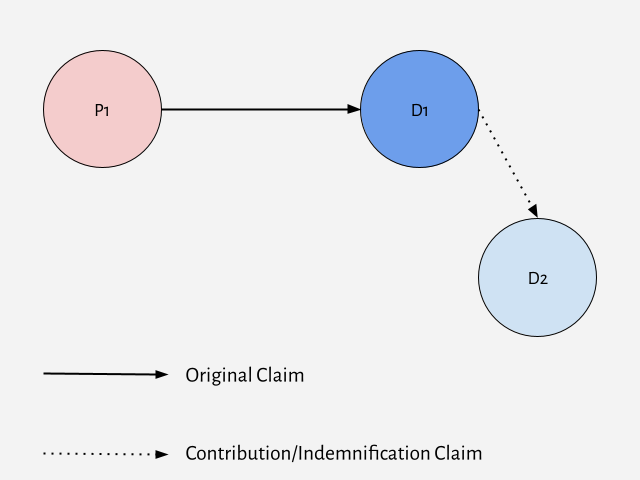
\includegraphics[width=0.66\linewidth,height=\textheight,keepaspectratio]{../img/Indemnification_Contribution.png}

}

\caption{Indemnification and Contribution}

\end{figure}%

D2 may already be a party to the lawsuit (i.e.~P1 has joined D2 as a
co-defendant under Rule 20), in which case D2 would assert a crossclaim
for indemnification or contribution under Rule 13(g). Or D2 may not yet
be a party, in which case D1 would join D2 as a third-party defendant
and assert a claim for indemnification or contribution under Rule 14(a).

D1's claim is functionally the same in either situation, but the FRCP
uses different terminology depending on how D2 becomes a party. Under
Rule 13(g), it is a cross-claim against a co-defendant; under Rule
14(a), it is a third-party claim against a third-party defendant.
Understanding that distinction (and using the correct terms) is
important, because it has other consequences under the FRCP: Rule 14
permits joinder of a third-party defendant \emph{only} to assert a claim
for indemnification or contribution on P's underlying claim, while Rule
13(g) would also permit crossclaims between D1 \& D2 for their direct
liability to each other arising from the same transaction or occurrence.

Under the FRCP, neither crossclaims nor third-party claims are
compulsory. Consequently, a party with a potential contribution or
indemnification claim (whether against a co-party or potential
third-party) may opt to wait until the outcome of the suit and then
bring the contribution/indemnification claim in a subsequent action.

Rules 13(g) and 14(a) do not establish a right to indemnification or
contribution. That is a matter of substantive law (tort, contract, or
statute). These Rules simply govern the procedure for joining such
claims where they have some basis in substantive law.

\subsubsection{Indemnification}\label{indemnification}

A right to indemnification allows a defending party to recover the full
amount of a judgment against them (and sometimes defense costs) from
another person. Indemnification originated as a common law right, based
on tort and agency law. The common law right has been augmented (or in
some jurisdictions replaced) by statutory and contractual rights to
indemnification.

\paragraph{Common Law Indemnification}\label{common-law-indemnification}

Common law indemnification applies where a defendant was not actually at
fault, but is liable to the plaintiff for another person's conduct,
based on their legal status or relationship.

\begin{itemize}
\item
  \emph{Example:} At common law, if an employer was held vicariously
  liable for harm to a third party caused by an employee, the employer
  could sue the employee for indemnification. In some states, this
  common law right to indemnification from employees has been abrogated
  by judicial opinion or statute.
\item
  \emph{Example:} In some states, if a retailer is subject to strict
  liability for injuries caused by a defective product it sold, the
  retailer has a common law right to indemnification by the manufacturer
  or other party actually responsible for the defect, as long as the
  retailer was not itself also at fault.
\end{itemize}

\paragraph{Statutory Indemnification}\label{statutory-indemnification}

Indemnification statutes may codify the common law right or impose a
duty to indemnify where it would not apply under common law.

\begin{itemize}
\item
  \emph{Example:} In some states, an employer has a statutory duty to
  indemnify an employee for civil liability arising from the employee's
  actions in the course of employment. See, e.g.,
  \href{https://leginfo.legislature.ca.gov/faces/codes_displaySection.xhtml?sectionNum=2802.&lawCode=LAB}{Cal.
  Labor Code §2802}.
\item
  \emph{Example:} The business corporations statutes in every state
  include provisions permitting (subject to certain conditions or
  limits) corporations to indemnify corporate officers and directors
  (and sometimes other employees and agents) who are sued based on their
  corporate roles. Some state's business corporations statutes mandate
  indemnification of officers and directors who successfully defend
  against such claims. See, e.g.,
  \href{https://delcode.delaware.gov/title8/c001/sc04/}{8 Del. Code
  §145}.
\end{itemize}

\paragraph{Contractual
Indemnification}\label{contractual-indemnification}

Parties may enter into agreements that shift ultimate responsibility for
judgments, without regard to which one is at fault.

\begin{itemize}
\item
  \emph{Example:} Many corporations enter into indemnification
  agreements with corporate officers and directors to provide
  indemnification for liability arising out of their corporate roles (as
  authorized by statute).
\item
  \emph{Example:} Manufacturers of consumer products may agree to
  indemnify distributors or retailers who face product liability suits.
  Such agreements may provide for indemnification where the common law
  right to indemnification does not apply or is not recognized at all
  under state law.
\end{itemize}

Liability insurance is a common type of contractual indemnification
agreement. Such policies typically provide that the insurance carrier
will pay (subject to limits and conditions in the policy) the cost of
judgments and the cost of defense for claims covered by the policy. If
there there is a dispute as to whether the policy covers the insured
party's potential liability, the insured party may join the insurance
carrier as a third-party defendant so that the court can resolve the
coverage dispute.

\subsubsection{Contribution}\label{contribution}

A right of contribution allows a joint tortfeasor who pays damages
beyond their proportionate share of fault (e.g.~under joint and several
liability) to seek reimbursement from other joint tortfeasors for their
proportionate shares. The right of contribution may be governed by
common law or statute. You will learn more about joint \& several
liability, and contribution among joint tortfeasers, in your Torts
class.

\subsection{Lehman v. Revolution Portfolio LLC (1st Cir.
1999)}\label{lehman-v.-revolution-portfolio-llc-1st-cir.-1999}

This appeal grows out of a triangular 1987 financial transaction that
involved the Farm Street Trust (the Trust), its beneficiaries (Barry
Lehman and Stuart A. Roffman), and First Mutual Bank for Savings (the
Bank). In the ensuing eleven years, the transaction imploded, litigation
commenced, the Bank and Lehman became insolvent, parties came and went,
and the case was closed and partially reopened. In the end, only a
third-party complaint proved ripe for adjudication. Even then, the
district court dismissed two of its three counts, but entered summary
judgment on the remaining count. The third-party defendant, Roffman, now
appeals. After sorting through the muddled record and the case's
serpentine procedural history, we affirm.

\subsubsection{Background}\label{background-1}

The historical facts are not seriously disputed. On or about October 19,
1987, the Trust, acting through its trustee, executed a promissory note
for \$2,800,000 in favor of the Bank in order to fund the purchase of
property in Dover, Massachusetts. Lehman and Roffman, each of whom
enjoyed a 50\% beneficial interest in the Trust, personally guaranteed
the note, and Lehman proffered two parcels of real estate as additional
collateral. In short order, the Trust defaulted on the loan and the Bank
foreclosed on Lehman's properties. Lehman responded by suing the Bank
seeking restraint or rescission of the imminent sale of his real estate.
The gravamen of his suit was a claim that Roffman had fraudulently
introduced a sham investor to the Bank in order to gull it into making
the loan, and that the Bank, in swallowing this spurious bait hook,
line, and sinker, had failed to exercise due diligence.

{[}\emph{The Bank failed and was placed in receivership. The FDIC, in
its role as receiver, replaced the Bank as defendant and asserted a
counterclaim against Lehman, as guarantor on the loan, to collect the
outstanding balance owed. The FDIC also joined Roffman as a third-party
defendant.}{]}

The FDIC's third-party complaint contained three counts. The first two
sought indemnification and contribution, respectively, in regard to the
claims advanced by Lehman. The third sought judgment against Roffman,
\emph{qua} guarantor, for the outstanding loan balance.

{[}\emph{Roffman moved to strike the third-party complaint. The trial
court denied that motion and Roffman appealed. Meanwhile, Revolution
Portfolio LLC (``RP''), to which the FDIC had assigned its interest in
the Farm Street Trust debt, replaced the FDIC as the real party in
interest.}{]}

\subsubsection{Discussion}\label{discussion-1}

We must answer the question whether the FDIC's deployment of a
third-party complaint against Roffman was proper. In this regard,
Roffman asserts that the district court should not have entertained the
impleader, and that, therefore, the joined claim on the guaranty should
fall of its own weight. We review a district court's decision to permit
the filing of a third-party complaint under Fed.R.Civ.P. 14(a) for abuse
of discretion.

As previously explained, the FDIC impleaded Roffman as a third-party
defendant on theories of indemnification and contribution (counts 1 and
2, respectively), maintaining, in essence, that if it were found to be
liable to Lehman, then Roffman would in turn be liable to hold it
harmless or, at least, contribute to any damages assessed against it. In
the same pleading, the FDIC asserted an independent claim for the
outstanding loan balance, premised on Roffman's guaranty (count 3). RP
(which now stands in the FDIC's shoes) acknowledges that the FDIC could
not have brought count 3 as a stand-alone third-party claim under Rule
14(a), but asserts that count 3 was validly joined with counts 1 and 2
under Fed.R.Civ.P. 18(a) (providing for permissive joinder). To parry
this thrust, Roffman contends that the FDIC's claims for indemnification
and contribution were not viable under state law, and thus, since the
use of Rule 14(a) admittedly hinged on the propriety of those claims,
the FDIC should not have been allowed to implead him at all.

We conclude, without serious question, that the FDIC was entitled to
implead Roffman under Rule 14(a) and that it appropriately joined the
guaranty claim under Rule 18(a).

A defendant, acting as a third-party plaintiff, may implead any
non-party ``who is or \emph{may be} liable to the third-party plaintiff
for all or part of the plaintiff's claim against the third-party
plaintiff.'' Fed.R.Civ.P. 14(a) (emphasis supplied). If the defendant
acts within ten days of submitting his answer, he may bring a third
party into the suit without leave of court. Otherwise, the court's
permission must be obtained. In that event, the determination is left to
the informed discretion of the district court, which should allow
impleader on any colorable claim of derivative liability that will not
unduly delay or otherwise prejudice the ongoing proceedings. Under this
liberal standard, a party accused of passive negligence (here, the FDIC)
assuredly is entitled to implead the party who allegedly committed the
relevant active conduct (here, Roffman) on a theory of indemnification.

The FDIC's third-party claim for contribution against Roffman similarly
passes muster because Roffman and the Bank (the FDIC's predecessor in
interest) were putative joint tortfeasors (i.e., according to the
complaint, Roffman's fraudulent acts combined with the Bank's negligent
omissions to create harm).

To be sure, Roffman argues that because Lehman's complaint sought only
restraint or rescission of the property sales, and not damages, a
third-party claim for contribution should not lie. But this argument
gains him no ground. Even though Lehman's complaint did not explicitly
seek money damages, that omission did not eliminate the possibility that
damages might be awarded to him. As long as damages may be awarded in
lieu of rescission, impleader properly may be used to seek contribution
toward those potential damages. It follows inexorably that the district
court did not err in denying Roffman's motion to strike and allowing the
FDIC's Rule 14(a) claims to stand.

Against this backdrop, the court properly assumed jurisdiction over
count 3 of the third-party complaint. Rule 18(a) authorizes a
third-party plaintiff to ``join, either as independent or as alternative
claims, as many claims, legal, equitable, or maritime, as the
{[}third-party plaintiff{]} has against an opposing party.'' This
authorization is subject only to the usual requirements of jurisdiction
and venue (none of which are implicated here) and the district court's
discretionary power to ``direct an appropriate procedure for trying the
claims.''. Given Rule 18(a)'s broad expanse, misjoinder of claims has
become an anachronism in federal civil practice.

In this instance, Roffman signed an unconditional personal guaranty of a
loan, and the borrower later defaulted. As a holder in due course of the
note, the FDIC had an independent claim for the outstanding balance
against Roffman. There is absolutely no reason why the FDIC could not
append its independent claim on the guaranty to its other claims against
Roffman.

As a fallback position, Roffman suggests that the third-party complaint
against him should have been dismissed because the FDIC had a complete
defense under 12 U.S.C. §1823(e) (1994) to the claims brought by Lehman.
We do not agree. Even if section 1823(e) offered the FDIC a potentially
strong defense against Lehman's claims, the record fails to show that
the mere existence of that statute rendered Lehman's complaint a
nullity.

There is, moreover, a broader point. A district court must oversee
third-party practice with the core purpose of Rule 14(a) in mind:
avoiding unnecessary duplication and circuity of action. Requiring a
district court to determine the merits of all defenses potentially
available to the original defendant as a precondition to allowing that
defendant to file a third-party complaint would frustrate this purpose
and countervail the efficient allocation of judicial resources. Thus, as
long as a third-party action falls within the general contours limned by
Rule 14(a), does not contravene customary jurisdictional and venue
requirements, and will not work unfair prejudice, a district court
should not preclude its prosecution. So here.

\subsection{Kirkcaldy v. Richmond County Bd. of Ed (M.D.N.C.
2002)}\label{kirkcaldy-v.-richmond-county-bd.-of-ed-m.d.n.c.-2002-1}

Until August of 2000, Smith served as a principal of the Leak Street
Alternative School, part of the Richmond County School System overseen
by the Board. On September 14, 2001, Plaintiff Elizabeth Kirkcaldy
(``Kirkcaldy''), who had worked as a secretary at the Leak Street
Alternative School, filed a lawsuit against Smith and the Board.
Kirkcaldy's Complaint alleges that from approximately July 20, 1999 to
June 12, 2000, she was subjected to sexual harassment by Smith, who
served as her direct supervisor during that time. Kirkcaldy claims that
during this time, Smith repeatedly made unwelcome sexual contact with
Kirkcaldy. Kirkcaldy also asserts that Smith frequently made comments of
a sexual nature to her. Based on these facts, Kirkcaldy asserts the
following claims: hostile work environment pursuant to 42 U.S.C. §2000e
et seq., intentional and negligent infliction of emotional distress
against both the Board and Smith, and a claim for negligent supervision,
retention and hiring against the Board.

In his Answer to Kirkcaldy's Complaint, Smith brings a cross-claim
against the Board and a third-party complaint against the Superintendent
of the Richmond County School System, Larry K. Weatherly
(``Weatherly''), and Board members Bruce Stanback, Sandy Lampley, Herman
Williams, Myrtle Stogner, Mary Carroll, Jackson Dawkins, and Carlene
Hill, all in their individual and official capacities. Smith's claim
against these Defendants is filed pursuant to 42 U.S.C. §1983 based on
the Individual School Defendants and the Board's (together, ``School
Defendants'') alleged violation of Smith's due process rights. It is
this Section 1983 claim that the School Defendants now move to dismiss.

In support of his claim, Smith asserts the following alleged facts. On
June 20, 2000, Weatherly informed Smith that he was being suspended with
pay while Weatherly investigated the allegations of sexual harassment
made by Kirkcaldy and another school employee, Sharon Renee Peek
(``Peek''). Based upon the results of this investigation, on July 25,
2000, Weatherly changed Smith's suspension with pay to suspension
without pay. Weatherly also informed Smith that a hearing before the
Board regarding Smith's employment would be held in August of 2000.
Weatherly further advised Smith that it would be recommended to the
Board members that they terminate Smith from his position.

Prior to the Board hearing, which was held on August 24, 2000, Weatherly
delivered to each Board member a copy of all the evidence he intended to
present at the hearing against Smith. This evidence included references
to polygraph examinations taken by Kirkcaldy and Peek. Smith asserts
that this evidence was inadmissible at a school board hearing under
North Carolina law. After reviewing the information provided to the
Board members, including the references to the polygraph examinations,
Myrtle Stogner, one of the Board members, allegedly made the statement
to an unidentified individual that the case against Smith was '' cut and
dried'' and that he would be dismissed for the alleged conduct.

At the August 24, 2000 hearing, Smith was allowed to present his
evidence. Smith proffered fourteen affidavits from witnesses that
rebutted the allegations of harassment made against Smith. Smith also
submitted his medical records and his wife's affidavit demonstrating
that he was impotent during the time period when the alleged harassment
occurred, and therefore would have been physically unable to engage in
some of the alleged misconduct. Smith requested a continuance of the
hearing in order to obtain additional evidence concerning his impotence,
but the Board denied his request.

At the conclusion of the August 24, 2000 hearing, the Board entered an
order dismissing Smith from his position as principal. Smith appealed
the Board's decision dismissing him to the North Carolina Superior
Court, which affirmed the Board's decision. Smith then appealed the
North Carolina Superior Court's decision to the North Carolina Court of
Appeals. This court affirmed the Superior Court's decision, which upheld
the Board's decision to dismiss Smith.

Smith's present cross-claim and third-party complaint filed pursuant to
Section 1983 claims that the School Defendants violated his due process
rights by denying him a fair hearing prior to his dismissal. In
response, the School Defendants have filed the Motion to Dismiss now
before the Court, asserting that dismissal of Smith's cross-claim and
third-party complaint is proper pursuant to Rule 12(b)(6) for failure to
state a claim and Rule 12(b)(1) for lack of subject-matter jurisdiction.

In addition to the Board's argument for dismissal of Smith's claim
against it, the School Defendants' Motion to Dismiss also requests that
the Court dismiss Smith's claim against the Individual School Defendants
because Smith's third-party complaint does not satisfy the
jurisdictional requirements of the Federal Rules of Civil Procedure. As
the Individual School Defendants, unlike the School Board itself, were
not parties to Kirkcaldy's original action, Smith's joinder of the
Individual School Defendants must meet the requirements of one of the
two Rules that allow the joinder of non-parties by a party defendant:
Rule 14(a), which governs the impleader of non-parties as third-party
defendants, or Rule 13(h), which governs the joinder of non-parties in
certain other situations.

As Smith has characterized his claim against the Individual School
Defendants as a third-party complaint, the Court will first consider
whether Smith's claim satisfies Rule 14(a), the Rule that authorizes the
addition of a third-party complaint to an action. Rule 14(a) allows a
defendant to assert, as a third-party complaint, a claim against a
person who is a non-party if that person is or may be liable to the
defendant for part or all of the plaintiff's claims against him. Turning
now to Smith's third-party complaint, the Court notes that it nowhere
asserts that the Individual School Defendants are liable to him for any
damages he might be responsible for due to Kirkcaldy's claims of sexual
harassment. Instead, Smith asserts a Section 1983 claim based on the
Individual School Defendants' actions regarding Smith's discharge. As
Smith's Section 1983 claim is not based on the secondary or derivative
liability of the Individual School Defendants, it cannot serve as the
basis for a third-party complaint. The Court therefore must conclude
that Smith has failed to satisfy Rule 14(a)'s requirements and cannot
use this Rule as the basis to join his claim against the Individual
School Defendants to Kirkcaldy's action.

In light of the Court's holding that Smith has not satisfied the
third-party practice requirements of Rule 14(a), Smith's claim as
alleged in his third-party complaint must be dismissed unless the claims
are authorized by Rule 13(h). Rule 13(h) allows a cross-defendant, when
asserting a cross-claim against another cross-defendant, to join to the
cross-claim persons who are not parties to the original action. It is
important to underscore, however, that Rule 13(h) imposes as a necessary
prerequisite that the cross-defendant first assert a claim against
another cross-claim defendant. Smith cannot meet this prerequisite
because of the Court's above decision dismissing his cross-claim against
the Board. As a result, Smith's Third-Party Complaint against the
Individual School Defendants can satisfy neither Rule 14(a) nor Rule
13(h) and therefore must also be dismissed. Accordingly, the Motion to
Dismiss for lack of subject matter jurisdiction is GRANTED to the
Individual School Defendants as well as to the School Board.

\section{Required Parties}\label{required-parties}

\subsection{Fed. R. Civ. P. Rule 19}\label{fed.-r.-civ.-p.-rule-19}

(a) Persons Required to Be Joined if Feasible.

\begin{itemize}
\item
  (1) Required Party. A person who is subject to service of process and
  whose joinder will not deprive the court of subject-matter
  jurisdiction must be joined as a party if:

  \begin{itemize}
  \item
    (A) in that person's absence, the court cannot accord complete
    relief among existing parties; or
  \item
    (B) that person claims an interest relating to the subject of the
    action and is so situated that disposing of the action in the
    person's absence may:

    \begin{itemize}
    \item
      (i) as a practical matter impair or impede the person's ability to
      protect the interest; or
    \item
      (ii) leave an existing party subject to a substantial risk of
      incurring double, multiple, or otherwise inconsistent obligations
      because of the interest.
    \end{itemize}
  \end{itemize}
\item
  (2) Joinder by Court Order. If a person has not been joined as
  required, the court must order that the person be made a party. A
  person who refuses to join as a plaintiff may be made either a
  defendant or, in a proper case, an involuntary plaintiff.
\item
  (3) Venue. If a joined party objects to venue and the joinder would
  make venue improper, the court must dismiss that party.
\end{itemize}

(b) When Joinder Is Not Feasible. If a person who is required to be
joined if feasible cannot be joined, the court must determine whether,
in equity and good conscience, the action should proceed among the
existing parties or should be dismissed. The factors for the court to
consider include:

\begin{itemize}
\item
  (1) the extent to which a judgment rendered in the person's absence
  might prejudice that person or the existing parties;
\item
  (2) the extent to which any prejudice could be lessened or avoided by:

  \begin{itemize}
  \item
    (A) protective provisions in the judgment;
  \item
    (B) shaping the relief; or
  \item
    (C) other measures;
  \end{itemize}
\item
  (3) whether a judgment rendered in the person's absence would be
  adequate; and
\item
  (4) whether the plaintiff would have an adequate remedy if the action
  were dismissed for nonjoinder.
\end{itemize}

(c) Pleading the Reasons for Nonjoinder. When asserting a claim for
relief, a party must state:

\begin{itemize}
\item
  (1) the name, if known, of any person who is required to be joined if
  feasible but is not joined; and
\item
  (2) the reasons for not joining that person.
\end{itemize}

\subsection{Camacho v. Major League Baseball (S.D. Cal.
2013)}\label{camacho-v.-major-league-baseball-s.d.-cal.-2013}

On November 30, 2012, Plaintiffs David Gonzalez Camacho and Daniel
Arrellano Pesqueira commenced this tort action against multiple
defendants. This action arises from allegations that Major League
Baseball conspired with the Mexican Major Leagues to prevent baseball
prospect Daniel Pesqueira from playing baseball in the United States.
Pending before the Court is the Office of the Commissioner of Baseball
(d/b/a Major League Baseball), Major League Baseball Enterprises, Inc.,
and Major League Baseball Properties, Inc.'s motion to dismiss pursuant
to Federal Rule of Civil Procedure 12(b)(7). Plaintiffs oppose the
motion.

The Court found this motion suitable for determination on the papers
submitted and without oral argument. For the following reasons, the
Court GRANTS Defendants' motion to dismiss.

\subsubsection[Background ]{\texorpdfstring{Background
\footnote{(n.3 in opinion) In the complaint, David Gonzalez Camacho is
  referred to as `Gonzalez,' and Daniel Arrellano Pesqueira, who is also
  once mentioned as `Daniel Pesqueira Arellano,' is referred to as
  `Pesqueira.' The Court will follow the same naming convention, and
  refer to the plaintiffs as Mr.~Gonzalez and Mr.~Pesqueira.}}{Background }}\label{background-camacho1}

Mr.~Gonzalez is a citizen of Mexico, ``who is domiciled and does
business in the City of Tijuana in the country of Mexico, and who does
business and resides in the County of San Diego, California, USA.'' He
is and was ``engaged in the training, support, promotion and
representation of young, talented and high caliber Mexican baseball
players for eventual placement in international major and minor leagues,
including Major and Minor League baseball conducted in the United
States.'' Mr.~Pesqueira is a citizen of Mexico who resides in Tijuana,
Mexico.

On April 1, 2010, Mr.~Gonzalez entered into an ``Exclusive Agency
Contract'' with Mr.~Pesqueira's parents on behalf of Mr.~Pesqueira, who
was a minor at the time. Under the agency contract, Mr.~Pesqueira
provided Mr.~Gonzalez with, among other things, the ``exclusive rights
to represent Pesqueira in the negotiation for and contracting of any and
all services of Pesqueira as a baseball player for any club in the major
and/or minor leagues of any and all countries at any level of play; and
Plaintiff Pesqueira agreed that Plaintiff Gonzalez would receive a 30\%
commission on any and all receipts and entitlements of Pesqueira for his
services as a baseball player for a three year term.'' Plaintiffs allege
that Mr.~Pesqueira is ``a young, talented, and burgeoning Mexican
baseball player who at all times relevant was and is a formidable left
handed pitcher.'' And pursuant to the terms of the contract,
Mr.~Gonzalez began to train and promote Mr.~Pesqueira, eventually
garnering the interest of talent scouts.

On February 17, 2012, the Boston Red Sox invited Mr.~Pesqueira to train
with the team for spring training in Fort Meyers, Florida. Then on March
6, 2012, a scout for the Boston Red Sox notified Mr.~Gonzalez that
Mr.~Pesqueira would be returned to Mexico ``based upon the direction of
Major League Baseball'' because Mr.~Pesqueira ``belonged to a Mexican
league team and could not play in the major leagues without the consent
of the Mexican league team.'' Plaintiffs dispute the validity of this
explanation, which they describe as a ``completely false'' premise.
Major League Baseball also advised Mr.~Gonzalez that Mr.~Pesqueira ``was
and is on the reserve list of the Association of Professional Baseball
Teams of the Mexican Leagues, therefore, he was ineligible to play for
the Boston Red Sox.''

At Mr.~Gonzalez's request, Major League Baseball forwarded a copy of the
``contractual documentation'' between Mr.~Pesqueira and the Mexican
League team called the Diablos Rojos (``Red Devils''). Plaintiffs
describe the documentation as containing ``two preprinted, form pages,
each prepared in Spanish,'' without any contractual terms. One
page---titled ``Contract for Professional Services''---includes
Mr.~Pesqueira's signature from January 1, 2010 with a start date of
March 22, 2009, and a second page with the same title includes
Mr.~Pesqueira's signature from and with a start date of March 21, 2011.
The former purportedly covers the 2009 Mexican baseball season, and the
latter covers the 2011 season. Plaintiffs allege that at both times
Mr.~Pesqueira was under 18 years old, having been born on April 6, 1994.
They also note that the earlier contract bears Mr.~Pesqueira's father
signature, though the later one does not.

According to Plaintiffs, Mr.~Pesqueira and his father confirmed that
they did not sign either of the documents provided by Major League
Baseball. They believe that ``either or both signatures of Pesqueira on
each document has or have been fraudulently lifted from another document
and transferred onto these documents, and that these documents are not
authentic.''

Sometime thereafter, Mr.~Gonzalez made a legal request to produce ``any
and all contracts or documents signed by Pesqueira, his parents or legal
representatives binding him in any way to the Red Devils, to any other
baseball team and/or to the Association of Professional Baseball Teams
of the Mexican Leagues.'' On February 23, 2011, the Association of
Professional Baseball Teams of the Mexican Leagues timely complied, and
produced a contract similar to the aforementioned ones. However, this
contract contained a signature of Mr.~Pesqueira dated January 1, 2010
with a March 22, 2010 start date, covering the 2010 Mexican baseball
season. Plaintiffs allege that Mr.~Pesqueira's signature on this
contract is the ``exact same signature'' as contained in the earlier
documents meant to cover the 2009 baseball season. Two other documents
were also produced: a document ``purported to be a Mexican Federal
Institute of Elections ID Card of Alberto Pesqueira Corrales, the
biological father of Pesqueira,'' and a ``purported copy of Pesqueira's
birth certificate.'' Plaintiffs allege that no documentation was
produced at the time pertaining to Mr.~Pesqueira and the 2011 Mexican
baseball season.

Plaintiffs continued their investigation. Either during or after the
investigation, Mr.~Gonzalez ``encouraged and facilitated efforts of
Major League Baseball to communicate and work with the Association of
Professional Baseball Teams of the Mexican Leagues and the Red Devils of
Mexico to verify that in fact Pesqueira was free to train and contract
with the Boston Red Sox or any other team.'' Plaintiffs allege that
Major League Baseball did indeed communicate with the Mexican League and
``confirmed that Pesqueira in fact was not committed to in any way, nor
under contract with, the Association of Professional Baseball Teams of
the Mexican Leagues and the Red Devils of Mexico.''

Plaintiffs commenced this action on November 30, 2012. They subsequently
amended their complaint after it was dismissed without prejudice for
lack of subject-matter jurisdiction. They assert the following claims
against all of the defendants for: (1) intentional interference with
economic relations; (2) intentional interference with prospective
economic advantage; (3) negligent interference with economic relations;
(4) negligent interference with prospective economic relations; (5)
declaratory relief; (6) negligence; and (7) unfair business practices.
Defendants now move to dismiss under Rule 12(b)(7). Plaintiffs oppose.

\subsubsection{Legal Standard}\label{legal-standard}

A party may move to dismiss a case for ``failure to join a party under
Rule 19.'' Fed. R. Civ. P. 12(b)(7). Rule 19 imposes a three-step
inquiry: (1) Is the absent party necessary (i.e., required to be joined
if feasible) under Rule 19(a)?; (2) If so, is it feasible to order that
absent party to be joined?; and (3) If joinder is not feasible, can the
case proceed without the absent party, or is the absent party
indispensable such that the action must be dismissed? The terms
``necessary'' and ``feasible'' are ``terms of art in Rule 19
jurisprudence'': ``Necessary'' refers to a party who should be joined if
feasible; and ``indispensable'' refers to ``a party whose participation
is so important to the resolution of the case that, if the joinder of
the party is not feasible, the suit must be dismissed.'' The failure to
join a party under Rule 19 can only lead to dismissal of a suit where
the court cannot obtain jurisdiction over the necessary party and that
party is determined to be indispensable to the action. \emph{See} Fed. R
.Civ. P. 19(a).

``The Ninth Circuit has held that a court should grant a 12(b)(7) motion
to dismiss only if the court determines that joinder would destroy
jurisdiction and the nonjoined party is necessary and indispensable.''
``A motion to dismiss for failure to join an indispensable party
requires the moving party to bear the burden in producing evidence in
support of the motion.'' ``A Rule 12(b)(7) motion for failure to join an
indispensable party demands a fact specific and practical inquiry.''
``To determine whether Rule 19 requires the joinder of additional
parties, the court may consider evidence outside the pleadings.''

\subsubsection{Discussion}\label{discussion-2}

Defendants argue that both the Red Devils and the Mexican League are
necessary parties that cannot be feasibl4y joined to this action because
(1) a determination of the validity of Mr.~Pesqueira's alleged contracts
with the Red Devils is necessary, and (2) joining the parties would
vitiate this Court's subject-matter jurisdiction and Plaintiffs cannot
establish personal jurisdiction over these absent parties in this Court.
Plaintiffs present their claims very differently in their opposition
brief compared to the allegations in the complaint. In a disingenuous
early-inning strategic shift, they direct the focus of this action on
Mr.~Gonzalez's agency contract with Mr.~Pesqueira, arguing that the Red
Devils and Mexican League are ``joint tortfeasors'' that are not
necessary parties to litigate the claims asserted in this action.
Plaintiffs swing for the fences, but ultimately come up short.

Upon reviewing the allegations in the complaint, it is clear that the
threshold issue in this action is the validity of the alleged contracts
entered into between Mr.~Pesqueira and the Red Devils. Plaintiffs
proceed with their action under the presumption that those contracts are
invalid---because Mr.~Pesqueira was a minor at the time the contracts
were executed, or because the signatures were ``fraudulently lifted from
another document and transferred onto these documents.'' These
allegations in the complaint overwhelmingly demonstrate that this entire
action hinges on one game-winning issue---the validity of the Red Devils
contracts. The Court emphasizes that determining the validity of the
alleged contracts between Mr.~Pesqueira and the Red Devils is outside
the scope of this series. Therefore, the Court rejects the disingenuous
shifted premise that Plaintiffs present in their opposition brief, and
shall proceed analyzing Defendants' motion while recognizing that the
validity of the alleged contracts entered into between Mr.~Pesqueira and
the Red Devils is the go-ahead run.

\paragraph{A. The Red Devils and the Mexican League Are Necessary
Parties.}\label{a.-the-red-devils-and-the-mexican-league-are-necessary-parties.}

A party is necessary if: (1) complete relief cannot be granted in the
party's absence; or (2) the district court determines that ``the absent
party's participation is necessary to protect its legally cognizable
interests or to protect other parties from a substantial risk of
incurring multiple or inconsistent obligations because of those
interests.'' Such a legally cognizable interest must be more than a
financial stake in the outcome of the litigation. Defendants demonstrate
that the Red Devils and the Mexican League are necessary parties under
the latter of the two aforementioned definitions.

Under Rule 19(a)(1)(B)(i), an absent party is necessary if it ``has a
\emph{legally protected interest} in the suit'' and ``that interest will
be \emph{impaired or impeded} by the suit.'' ``Impairment may be
minimized if the absent party is adequately represented in the suit.''
\emph{Id.} It is also a ``fundamental principle'' that ``a party to a
contract is necessary, and if not susceptible to joinder, indispensable
to litigation seeking to decimate that contract.''

Plaintiffs unequivocally seek a judicial determination of their rights
and duties under the alleged contracts between Mr.~Pesqueira and the Red
Devils. In the complaint, Plaintiffs explicitly state that they desire
``a declaration as to whether or not Pesqueira is bound to the Red
Devils of Mexico.'' They even go as far as to state that a ``judicial
declaration is \emph{necessary} and appropriate at this time under the
circumstances'' because without the declaration, they are ``financially
burdened by the wrongful position taken by defendants Major League
Baseball, and unable to work in their chosen professions.'' In other
words, determining the validity of the Red Devils contracts is necessary
to resolve essentially all of the wrongful conduct alleged in this
action. The same applies to the Mexican League because of its bylaws and
regulations that require disputes between players and member teams to be
resolved by binding arbitration before the Executive President of the
Mexican League.

Neither the Red Devils nor the Mexican League are represented in this
action, and a determination by this Court regarding the validity of the
Red Devils contracts may impair and impede the Red Devils' and the
Mexican League's legally protected interest in this suit. Keeping with
the baseball theme, a batter cannot record a base hit or a home run
against an absent pitcher; that pitcher needs to be in the game before
that happens. In this circumstance, the absent pitchers are the Red
Devils and the Mexican League. Therefore, as a party to the Red Devils
contracts, the Red Devils, and by extension the Mexican League, are
necessary parties.

Alternatively, under Rule 19(a)(1)(B)(ii), an absent party is also
necessary if there is a potential risk that adjudicating an action
without the absent party could leave an existing party open to
``incurring double, multiple, or otherwise inconsistent obligations.''
Fed. R. Civ. P. 19(a)(1)(B)(ii). The Ninth Circuit has stated that

\begin{quote}
``inconsistent obligations'' are not the same as inconsistent
adjudications or results. Inconsistent obligations occur when a party is
unable to comply with one court's order without breaching another
court's order concerning the same incident. Inconsistent adjudications
or results, by contrast, occur when a defendant successfully defends a
claim in one forum, yet loses on another claim arising from the same
incident in another forum.
\end{quote}

Defendants argue that ``the Red Devils could still sue others in the
Mexican courts and elsewhere for wrongfully interfering with its
contract with Mr.~Pesqueira,'' and ``this action will not have any
binding effect on the Red Devils unless the team is made a party to this
case.'' (Defs.' Mot. 11:10-19.) The concern that Defendants suggest is
important, but for the purposes of Rule 19, the paramount concern is a
Mexican court or another in the United States determining that the Red
Devils contracts are valid if this Court finds that they are not, or
vice versa. That would produce inconsistent obligations for all of the
parties in this action in addition to the Red Devils because operating
under one court's determination would then necessarily cause the parties
to breach another court's determination regarding the same issue, i.e.,
the validity of the Red Devils contracts. Therefore, because of the risk
of inconsistent obligations, the Red Devils are a necessary party to
this action.

Swing and a miss---strike one.

\paragraph{B. Joining the Red Devils and the Mexican League Is Not
Feasible.}\label{b.-joining-the-red-devils-and-the-mexican-league-is-not-feasible.}

``If an absentee is a necessary party under Rule 19(a), the second stage
is for the court to determine whether it is feasible to order that the
absentee be joined.'' Rule 19(a) sets forth three circumstances in which
joinder is not feasible: (1) when venue is improper; (2) when the
absentee is not subject to personal jurisdiction; and (3) when joinder
would destroy subject matter jurisdiction.

Defendants argue that ``the Red Devils and the Mexican League cannot be
joined both because their joinder would destroy this Court's
subject-matter jurisdiction, and because Plaintiffs cannot establish
personal jurisdiction over them in this Court.'' Plaintiffs do not
address feasibility in their opposition brief. In fact, the words
``feasible'' and ``feasibility'' do not appear anywhere in their brief.
Consequently, Plaintiffs concede that joining the Red Devils and the
Mexican League is not feasible under the second and third circumstances
that Rule 19 enumerates. They took this pitch and it went right down the
middle---strike two.

\paragraph{C. The Red Devils and Mexican League Are Indispensable
Parties.}\label{c.-the-red-devils-and-mexican-league-are-indispensable-parties.}

If the necessary party cannot be joined, the court must then determine
whether the party is indispensable. Under Rule 19(b), indispensable
parties are ``persons who not only have an interest in the controversy,
but an interest of such a nature that a final decree cannot be made
without either affecting that interest, or leaving the controversy in
such a condition that its final termination may be wholly inconsistent
with equity and good conscience.'' Rule 19(b) provides the factors that
courts should consider in determining if an action should be dismissed
because an absent party is indispensable: (1) prejudice to any party or
to the absent party; (2) whether relief can be shaped to lessen
prejudice; (3) whether an adequate remedy, even if not complete, can be
awarded without the absent party; and (4) whether there exists an
alternative forum. Furthermore, ``no procedural principle is more deeply
imbedded in the common law than that, in an action to set aside a lease
or a contract, all parties who may be affected by the determination of
the action are indispensable.''

Plaintiffs' primary arguments addressing indispensability are: (1)
Defendants fail to meet their burden, in part, because all of the cases
cited are distinguishable, and (2) in equity and good conscience, this
case should be allowed to proceed regardless of whether the Red Devils
and the Mexican League are indispensable. The Court rejects these
arguments. Plaintiffs either misread or misunderstand the cited case
law, and they also fail to provide any law themselves that provides an
avenue for this Court to bypass Rules 12(b)(7) and 19 and all of the
related case law as they implore the Court do.

Rather, in seeking a determination that the Red Devils contracts are
invalid, Plaintiffs are, for all practical purposes, attempting to set
aside a contract. And it is evident from the allegations in the
complaint that the Red Devils, as a party to the alleged contracts, and
by extension the Mexican League, are parties that will be affected by
any determination regarding the validity of the contracts. If Plaintiffs
want to record an earned run against the absent pitchers, Plaintiffs
need to face them. Thus, the Red Devils and the Mexican League are
indispensable parties to this action. Consequently, all four of the Rule
19(b) factors weigh in favor of dismissal. And finally, strike
three---out.

\subsection{Sullivan-Blake v. Fedex Ground Package System, Inc.~(W.D.
Pa.
2020)}\label{sullivan-blake-v.-fedex-ground-package-system-inc.-w.d.-pa.-2020}

Pending before the Court in this collective action under the Fair Labor
Standards Act (``FLSA'') is FedEx Ground Package System, Inc.'s
(``FedEx'') Rule 19(a) Motion to Join Pennsylvania Service Providers as
Necessary Parties and Rule 19(b) Motion to Dismiss for Failure to Join
Indispensable Parties (the ``Motion''). In its Motion, FedEx seeks the
joinder in this action of companies within Pennsylvania that contracted
with FedEx to provide delivery and pickup services (``Service
Providers'') and dismissal of the remainder of the case as it pertains
to opt-in Plaintiffs residing outside of Pennsylvania and Service
Providers who employed drivers outside of Pennsylvania.

\subsubsection{Relevant Background}\label{relevant-background}

Plaintiffs Angel Sullivan-Blake and Horace Claiborne claim that they
were not paid overtime compensation in accordance with the FLSA and have
brought this collective action on behalf of themselves and other
similarly situated individuals who have been employed by FedEx through
intermediary employers, that is, the Service Providers, to perform
delivery services on FedEx's behalf. To date, fifty-seven individuals
from twenty-six different states have filed their opt-in consent forms
to join this action.

On September 30, 2019, the Court conditionally certified a nationwide
collective encompassing all individuals outside of Massachusetts who
worked as FedEx delivery drivers through the Service Providers since
November 27, 2015. Before notice was issued to potential collective
members, FedEx filed the pending Motion which has been fully briefed and
is ripe for disposition.

\subsubsection{Discussion}\label{discussion-3}

FedEx contends that all Service Providers nationwide are necessary and
indispensable parties to this litigation because these providers employ
and pay the drivers, set the employment and wage policies and have a
direct interest in the outcome. As such, FedEx seeks to join Service
Providers located in Pennsylvania as required parties pursuant to Rule
19(a) of the Federal Rules of Civil Procedure. FedEx further asserts
that because the Court lacks jurisdiction over the non-Pennsylvania
Service Providers who employed Plaintiffs as well as opt-in Plaintiffs
residing outside of Pennsylvania, then pursuant to Rule 19(b), these
claims must be dismissed since these parties are indispensable and
joinder cannot be effected.

``To be an indispensable party under Federal Rule of Civil Procedure
Rule 19(b), a party must also be a `required' party under Rule 19(a).''
Accordingly, the starting point of the Court's analysis is whether the
Service Providers are ``required'' parties under Rule 19(a) because
``Rule 19(b) itself is applicable only if a person who should be joined
under the provisions of Rule 19(a) cannot be made a party for some
reason.''

Rule 19(a) classifies an absent party as a ``required party'' and
mandates its joinder, if feasible, in three situations. Fed. R. Civ. P.
19(a)(1). First, if ``the court cannot accord complete relief among
existing parties,'' without the joinder of the absentee. Fed. R. Civ. P.
19(a)(1)(A). Second, if the absentee ``claims an interest relating to
the subject of the action and is so situated that disposing of the
action'' without its joinder may ``as a practical matter impair or
impede the absentee's ability to protect the interest.'' Fed. R. Civ. P.
19(a)(1)(B)(i). Finally, if the absentee ``claims an interest relating
to the subject of the action and is so situated that disposing of the
action'' without joining the absentee may, ``leave an existing party
subject to a substantial risk of incurring double, multiple, or
otherwise inconsistent obligations because of the interest.'' Fed. R.
Civ. P. 19(a)(1)(B)(ii).

Contrary to FedEx's assertions, none of these situations are applicable
here.

Under Rule 19(a)(1)(A), ``the Court must consider whether---in the
absence of an un-joined party---complete relief can be granted to the
persons already parties to the lawsuit.'' FedEx asserts that the Service
Providers are ``required'' parties pursuant to this provision because it
is the Service Providers, and not FedEx, that are ``the employers
responsible for compensation, and Plaintiffs cannot achieve complete
relief without their participation.'' This assertion is without merit,
however, because ``under the FLSA, multiple persons or entities can be
responsible for a single employee's wages as `joint employers' in
certain situations. Indeed, FedEx acknowledges that this is a joint
employment case.

In such cases, ``each joint employer may be held jointly and severally
liable for the FLSA violations of the other, in addition to direct
liability for its own violations.'' If Plaintiffs prevail in this case
and FedEx is deemed a joint employer under the FLSA, it will be
individually liable to Plaintiffs for all damages. Thus, because the
Court can accord complete relief among the existing parties, the Service
Providers are not ``required'' parties under Rule
19(a)(1)(A).\footnote{(n.1 in opinion) FedEx also contends that
  Plaintiffs cannot obtain complete relief without the joinder of the
  Service Providers because if Plaintiffs cannot prove that FedEx is
  their joint employer, their FLSA claims against the Service Providers
  would likely be time barred. This contention is irrelevant to the
  Court's analysis, however, because the focal point of the inquiry
  under Rule 19(a)(1)(A) is whether the Court can accord complete relief
  if Plaintiffs prevail in \emph{this} litigation. Similarly, FedEx's
  assertion that the Court cannot accord complete relief to FedEx
  because the indemnification agreements between itself and the Service
  Providers may lead to future litigation does not compel joinder.
  Whether the Court can accord complete relief ``is determined on the
  basis of those persons who are already parties, and not as between a
  party and the absent person whose joinder is sought.''}

Under Rule 19(a)(1)(B)(i), ``the court must decide whether determination
of the rights of those persons named as parties to the action would
impair or impede an absent party's ability to protect its interest in
the subject matter of the litigation.'' FedEx asserts that the Service
Providers are ``required'' parties pursuant to this provision for two
reasons.

First, FedEx argues that Plaintiffs' allegations implicate the Service
Providers' pay practices and compensation structures. According to
FedEx, any imposition of FLSA liability in this case will compel the
absentee Service Providers to change their pay practices or risk being
sued by their current employees for additional FLSA violations. Second,
FedEx contends that the Service Providers have a direct interest in
defending their pay practices because they have an indemnification
agreement with FedEx.

Both of these arguments miss the mark because in order for the Service
Providers to be classified as ``required'' parties under Rule
19(a)(1)(B)(i), FedEx must show that ``some outcome of the federal case
that is reasonably likely can preclude the absent party with respect to
an issue material to the absent party's rights or duties under standard
principles governing the effect of prior judgments.'' The requirements
of this provision are ``not satisfied simply because a judgment against
FedEx in this action might set a persuasive precedent in any potential
future action against the absentee Service Providers.'' At this
juncture, it would be premature for this Court to determine what effect,
if any, an adverse judgment against FedEx in this case may have on
subsequent, yet to be filed, lawsuits against the Service Providers
brought either by Plaintiffs or FedEx. Because the Service Providers do
not have a direct stake in this litigation, they are not ``required''
parties under Rule 19(a)(1)(B).

Under Rule 19(a)(2)(ii), ``a court must decide whether continuation of
the action would expose named parties to the substantial risk of
incurring double, multiple, or otherwise inconsistent obligations by
reason of the absentee's claimed interest.'' FedEx asserts that the
Service Providers are ``required'' parties pursuant to this provision
because their absence may subject FedEx to inconsistent obligations. It
argues that if it is found liable in this litigation, it might bring
indemnification proceedings against the Service Providers and because
the outcome of this litigation may not bind the Service Providers in
those indemnification proceedings, inconsistent obligations may follow.
FedEx's argument fails for two reasons.

First, Rule 19(a)(1)(B)(ii) ``protects against inconsistent obligations,
not inconsistent adjudications; under the Rule a person is protected
against situations in which there would be two court orders and
compliance with one might breach the other.'' That is not the case here.
Second, the possibility that FedEx ``may have to shoulder the entire
loss if found liable is a necessary consequence of joint and several
liability.'' Accordingly, the Service Providers are not ``required''
parties under Rule 19(a)(1)(B)(ii).

In short, the Service Providers are not ``required'' parties under any
of the provisions of Rule 19(a). Because the threshold requirements Rule
19(a) are not met, it is therefore unnecessary for the Court to conduct
a Rule 19(b) analysis.

\section{Review Questions}\label{review-questions}

Mrs.~Claypool, an aspiring society matron, hears that the director of
the New York Opera Company, Herman Gottlieb, is seeking a patron.
Claypool believes this is a perfect way to enhance her standing in
society. She hires Otis Driftwood to act as her agent in negotiating a
deal with Gottlieb, under which Claypool will donate \$500,000 to the
Opera Company so it can hire Rodolfo Lassparri, the greatest tenor in
the world. In exchange, Gottlieb agrees to name the Opera House after
Claypool.

Driftwood goes to meet Lassparri, intending to sign him to a contract
with the Opera Company to close the deal between Claypool \& Gottlieb.
Along the way, he meets Fiorello, a genial con artist, who tricks
Driftwood into signing Lassparri's rival, Baroni, instead. When Gottlieb
discovers what has happened, he renegs on his agreement to name the
Opera House after Claypool.

A furious Claypool sues Gottlieb for breach of contract, seeking
restitution of the \$500,000 she donated to the Opera Company. She also
sues Driftwood for breach of contract \& fraud over his role in the
failure of the Opera Company deal, seeking \$50,000 (the amount she paid
Driftwood for his services as her agent) plus punitive damages. Claypool
brings her suit in federal court (assume that the court would have
personal jurisdiction over all parties and subject matter jurisdiction
over all claims).

\subsubsection{Part A}\label{part-a}

\begin{enumerate}
\def\labelenumi{\arabic{enumi}.}
\item
  Is joinder of Gottlieb and Driftwood as defendants proper under the
  FRCP?
\item
  Assume that Claypool sues only Gottlieb. Gottlieb's defense is that
  his promise to name the Opera House after Claypool was contingent upon
  signing Lasparri to a contract with the Opera Company, and that
  Driftwood's failure to fulfill that part of the deal means that
  Gottlieb is not contractually obligated to honor his promise to
  Claypool. Is Driftwood a person required to be joined if feasible
  under the FRCP?
\item
  Assume instead that Claypool sues only Dritwood. May Gottlieb
  intervene as a plaintiff to assert a claim against Driftwood for
  failure to sign Lasparri to a contract with the Opera Company?
\end{enumerate}

\subsubsection{Part B}\label{part-b}

Assume that Claypool sued both Gottlieb \& Driftwood and that their
joinder as co-defendants was proper under the FRCP.

For each of the following additional claims, explain whether joinder is
proper under the FRCP:

\begin{enumerate}
\def\labelenumi{\arabic{enumi}.}
\item
  A claim by Driftwood against Claypool for breach of contract, seeking
  \$25,000 he contends she still owes him for his services under their
  contract.
\item
  A claim by Driftwood against Claypool for battery, alleging that she
  poured a bowl of hot soup over his head when he clumsily attempted to
  woo her during a party to celebrate the ill-fated Opera deal.
\item
  A claim by Gottlieb against Driftwood, alleging that the Opera Company
  lost 50\% of its anticipated season ticket sales because of the
  failure to sign Lassparri.
\item
  A claim by Gottlieb against Driftwood for breach of contract in an
  unrelated business transaction in which Driftwood was to supply the
  Opera Company with costumes.
\item
  A claim by Driftwood against Fiorello and Baroni, asserting that if
  Driftwood is found liable to Claypool or Gottlieb for his failure to
  sign Lasparri, Fiorello and Baroni must cover all or part of any
  damages Driftwood is ordered to pay Claypool or Gottlieb, because it
  was their fault Driftwood failed to sign Lasparri.
\item
  A claim by Driftwood against Fiorello and Baroni, seeking \$25,000
  against them, jointly and severally, for defrauding him into signing
  Baroni to the Opera contract. The \$25,000 represents the commission
  Driftwood expected to earn by signing Lasparri.
\item
  A claim by Baroni against Driftwood for failure to pay Baroni in
  accordance with the contract that Driftwood signed.
\end{enumerate}

\begin{figure}[H]

{\centering 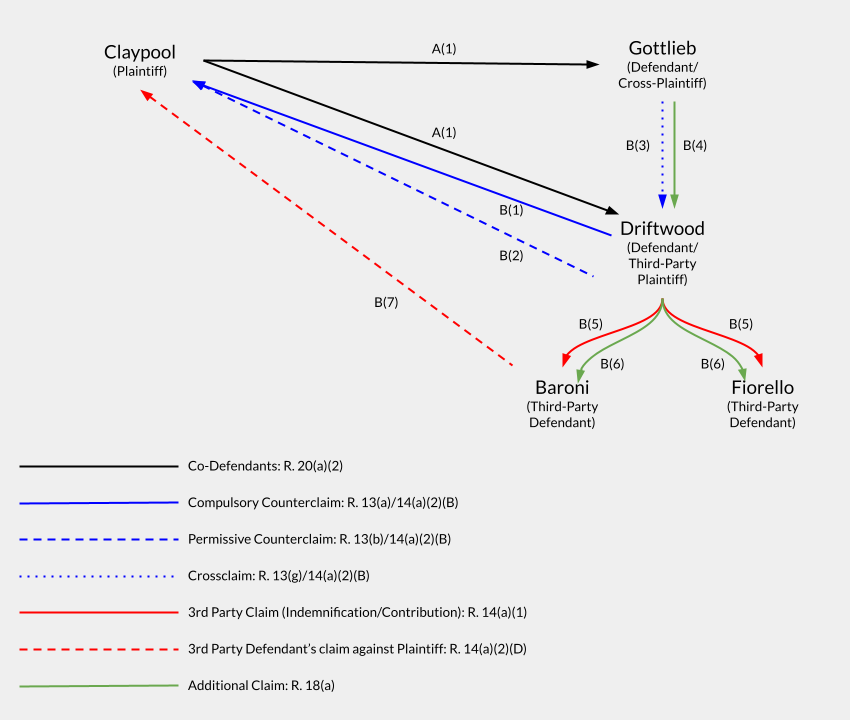
\includegraphics[width=0.75\linewidth,height=\textheight,keepaspectratio]{../img/JoinderProblem.png}

}

\caption{Parties \& Claims in Claypool v. Gottlieb}

\end{figure}%

\chapter{Personal Jurisdiction}\label{personal-jurisdiction}

\section{Constitutional Limits: Due
Process}\label{constitutional-limits-due-process}

\subsection{U.S. Constitution,}\label{u.s.-constitution}

\subsubsection{Amendment V}\label{amendment-v}

No person shall \ldots{} be deprived of life, liberty, or property,
without due process of law; \ldots.

\subsubsection{Amendment XIV, sec.~1}\label{amendment-xiv-sec.-1}

\ldots{} nor shall any state deprive any person of life, liberty, or
property, without due process of law; \ldots.

\subsection{Pennoyer v. Neff (U.S.
1878)}\label{pennoyer-v.-neff-u.s.-1878}

\subsubsection{Justice Field delivered the opinion of the
court.}\label{justice-field-delivered-the-opinion-of-the-court.}

This is an action to recover the possession of a tract of land, of the
alleged value of \$15,000, situated in the State of Oregon. The
plaintiff asserts title to the premises by a patent of the United States
issued to him in 1866, under the act of Congress of Sept.~27, 1850,
usually known as the Donation Law of Oregon. The defendant claims to
have acquired the premises under a sheriff's deed, made upon a sale of
the property on execution issued upon a judgment recovered against the
plaintiff in one of the circuit courts of the State. The case turns upon
the validity of this judgment.

It
{\marginnote{\begin{footnotesize}\pandocbounded{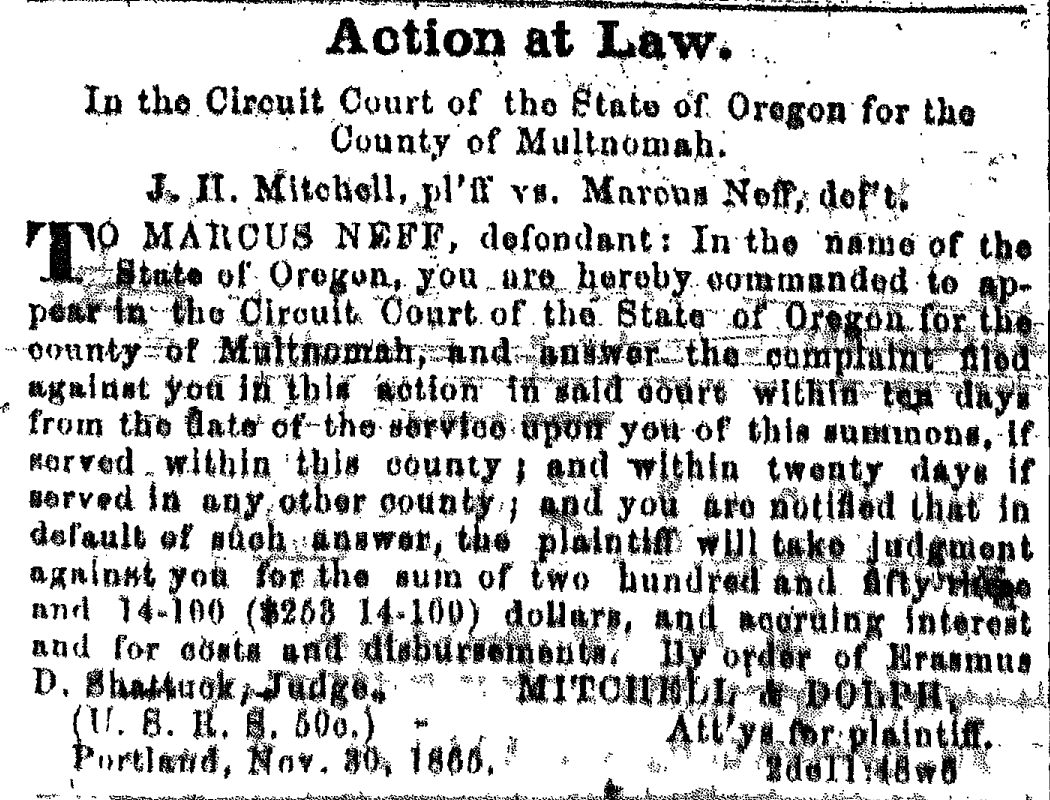
\includegraphics[keepaspectratio]{../img/mitchell-neff-notice.png}}
Notice by publication in Mitchell v. Neff (\emph{Pacific Christian
Advocate}, Portland, Oregon, Dec.~2, 1865)\end{footnotesize}}} appears
from the record that the judgment was rendered in February, 1866, in
favor of J.H. Mitchell, for less than \$300, including costs, in an
action brought by him upon a demand for services as an attorney; that,
at the time the action was commenced and the judgment rendered, the
defendant therein, the plaintiff here, was a non-resident of the State;
that he was not personally served with process, and did not appear
therein; and that the judgment was entered upon his default in not
answering the complaint, upon a constructive service of summons by
publication.

The Code of Oregon provides for such service when an action is brought
against a non-resident and absent defendant, who has property within the
State. It also provides, where the action is for the recovery of money
or damages, for the attachment of the property of the non-resident. And
it also declares that no natural person is subject to the jurisdiction
of a court of the State, ``unless he appear in the court, or be found
within the State, or be a resident thereof, or have property therein;
and, in the last case, only to the extent of such property at the time
the jurisdiction attached.'' Construing this latter provision to mean,
that, in an action for money or damages where a defendant does not
appear in the court, and is not found within the State, and is not a
resident thereof, but has property therein, the jurisdiction of the
court extends only over such property, the declaration expresses a
principle of general, if not universal, law. The authority of every
tribunal is necessarily restricted by the territorial limits of the
State in which it is established. Any attempt to exercise authority
beyond those limits would be deemed in every other forum, as has been
said by this court, an illegitimate assumption of power, and be resisted
as mere abuse. In the case against the plaintiff, the property here in
controversy sold under the judgment rendered was not attached, nor in
any way brought under the jurisdiction of the court. Its first
connection with the case was caused by a levy of the execution. It was
not, therefore, disposed of pursuant to any adjudication, but only in
enforcement of a personal judgment, having no relation to the property,
rendered against a non-resident without service of process upon him in
the action, or his appearance therein. The court below did not consider
that an attachment of the property was essential to its jurisdiction or
to the validity of the sale, but held that the judgment was invalid from
defects in the affidavit upon which the order of publication was
obtained, and in the affidavit by which the publication was proved.

It was also contended in that court,
{\marginnote{\begin{footnotesize}``In-rem jurisdiction refers to the
power of a court over an item of real or personal property. In-rem
jurisdiction is based on the location of the property and enforcement
follows property rather than person.''
\href{https://www.law.cornell.edu/wex/in_rem}{Wex Legal
Dictionary}.\end{footnotesize}}} and is insisted upon here, that the
judgment in the State court against the plaintiff was void for want of
personal service of process on him, or of his appearance in the action
in which it was rendered, and that the premises in controversy could not
be subjected to the payment of the demand of a resident creditor except
by a proceeding \emph{in rem}; that is, by a direct proceeding against
the property for that purpose. If these positions are sound, the ruling
of the Circuit Court as to the invalidity of that judgment must be
sustained, notwithstanding our dissent from the reasons upon which it
was made. And that they are sound would seem to follow from two
well-established principles of public law respecting the jurisdiction of
an independent State over persons and property. The several States of
the Union are not, it is true, in every respect independent, many of the
rights and powers which originally belonged to them being now vested in
the government created by the Constitution. But, except as restrained
and limited by that instrument, they possess and exercise the authority
of independent States, and the principles of public law to which we have
referred are applicable to them. One of these principles is, that every
State possesses exclusive jurisdiction and sovereignty over persons and
property within its territory. As a consequence, every State has the
power to determine for itself the civil status and capacities of its
inhabitants; to prescribe the subjects upon which they may contract, the
forms and solemnities with which their contracts shall be executed, the
rights and obligations arising from them, and the mode in which their
validity shall be determined and their obligations enforced; and also to
regulate the manner and conditions upon which property situated within
such territory, both personal and real, may be acquired, enjoyed, and
transferred. The other principle of public law referred to follows from
the one mentioned; that is, that no State can exercise direct
jurisdiction and authority over persons or property without its
territory. The several States are of equal dignity and authority, and
the independence of one implies the exclusion of power from all others.
And so it is laid down by jurists, as an elementary principle, that the
laws of one State have no operation outside of its territory, except so
far as is allowed by comity; and that no tribunal established by it can
extend its process beyond that territory so as to subject either persons
or property to its decisions.

But as contracts made in one State may be enforceable only in another
State, and property may be held by non-residents, the exercise of the
jurisdiction which every State is admitted to possess over persons and
property within its own territory will often affect persons and property
without it. To any influence exerted in this way by a State affecting
persons resident or property situated elsewhere, no objection can be
justly taken; whilst any direct exertion of authority upon them, in an
attempt to give ex-territorial operation to its laws, or to enforce an
ex-territorial jurisdiction by its tribunals, would be deemed an
encroachment upon the independence of the State in which the persons are
domiciled or the property is situated, and be resisted as usurpation.

Thus the State, through its tribunals, may compel persons domiciled
within its limits to execute, in pursuance of their contracts respecting
property elsewhere situated, instruments in such form and with such
solemnities as to transfer the title, so far as such formalities can be
complied with; and the exercise of this jurisdiction in no manner
interferes with the supreme control over the property by the State
within which it is situated.

So the State, through its tribunals, may subject property situated
within its limits owned by non-residents to the payment of the demand of
its own citizens against them; and the exercise of this jurisdiction in
no respect infringes upon the sovereignty of the State where the owners
are domiciled. Every State owes protection to its own citizens; and,
when non-residents deal with them, it is a legitimate and just exercise
of authority to hold and appropriate any property owned by such
non-residents to satisfy the claims of its citizens. It is in virtue of
the State's jurisdiction over the property of the non-resident situated
within its limits that its tribunals can inquire into that
non-resident's obligations to its own citizens, and the inquiry can then
be carried only to the extent necessary to control the disposition of
the property. If the non-resident have no property in the State, there
is nothing upon which the tribunals can adjudicate.

If, without personal service, judgments in
personam,{\marginnote{\begin{footnotesize}``In personam refers to
courts' power to adjudicate matters directed against a party, as
distinguished from in-rem proceedings over disputed property.''
\href{https://www.law.cornell.edu/wex/in_personam}{Wex Legal
Dictionary}.\end{footnotesize}}} obtained ex parte against non-residents
and absent parties, upon mere publication of process, which, in the
great majority of cases, would never be seen by the parties interested,
could be upheld and enforced, they would be the constant instruments of
fraud and oppression. Judgments for all sorts of claims upon contracts
and for torts, real or pretended, would be thus obtained, under which
property would be seized, when the evidence of the transactions upon
which they were founded, if they ever had any existence, had perished.
{\marginnote{\begin{footnotesize}``In civil procedure, ex parte is used
to refer to motions for orders that can be granted without waiting for a
response from the other side. Generally, these are orders that are only
in place until further hearings can be held, such as a temporary
restraining order.'' \href{https://www.law.cornell.edu/wex/ex_parte}{Wex
Legal Dictionary}.\end{footnotesize}}}

Substituted service by publication, or in any other authorized form, may
be sufficient to inform parties of the object of proceedings taken where
property is once brought under the control of the court by seizure or
some equivalent act. The law assumes that property is always in the
possession of its owner, in person or by agent; and it proceeds upon the
theory that its seizure will inform him, not only that it is taken into
the custody of the court, but that he must look to any proceedings
authorized by law upon such seizure for its condemnation and sale. Such
service may also be sufficient in cases where the object of the action
is to reach and dispose of property in the State, or of some interest
therein, by enforcing a contract or a lien respecting the same, or to
partition it among different owners, or, when the public is a party, to
condemn and appropriate it for a public purpose. In other words, such
service may answer in all actions which are substantially proceedings in
rem. But where the entire object of the action is to determine the
personal rights and obligations of the defendants, that is, where the
suit is merely in personam, constructive service in this form upon a
non-resident is ineffectual for any purpose. Process from the tribunals
of one State cannot run into another State, and summon parties there
domiciled to leave its territory and respond to proceedings against
them. Publication of process or notice within the State where the
tribunal sits cannot create any greater obligation upon the non-resident
to appear. Process sent to him out of the State, and process published
within it, are equally unavailing in proceedings to establish his
personal liability.

The want of authority of the tribunals of a State to adjudicate upon the
obligations of non-residents, where they have no property within its
limits, is not denied by the court below: but the position is assumed,
that, where they have property within the State, it is immaterial
whether the property is in the first instance brought under the control
of the court by attachment or some other equivalent act, and afterwards
applied by its judgment to the satisfaction of demands against its
owner; or such demands be first established in a personal action, and
the property of the non-resident be afterwards seized and sold on
execution. But the answer to this position has already been given in the
statement, that the jurisdiction of the court to inquire into and
determine his obligations at all is only incidental to its jurisdiction
over the property. Its jurisdiction in that respect cannot be made to
depend upon facts to be ascertained after it has tried the cause and
rendered the judgment. If the judgment be previously void, it will not
become valid by the subsequent discovery of property of the defendant,
or by his subsequent acquisition of it. The judgment if void when
rendered, will always remain void: it cannot occupy the doubtful
position of being valid if property be found, and void if there be none.
Even if the position assumed were confined to cases where the
non-resident defendant possessed property in the State at the
commencement of the action, it would still make the validity of the
proceedings and judgment depend upon the question whether, before the
levy of the execution, the defendant had or had not disposed of the
property. If before the levy the property should be sold, then,
according to this position, the judgment would not be binding. This
doctrine would introduce a new element of uncertainty in judicial
proceedings. The contrary is the law: the validity of every judgment
depends upon the jurisdiction of the court before it is rendered, not
upon what may occur subsequently.

The force and effect of judgments rendered against non-residents without
personal service of process upon them, or their voluntary appearance,
have been the subject of frequent consideration in the courts of the
United States and of the several States, as attempts have been made to
enforce such judgments in States other than those in which they were
rendered, under the provision of the Constitution requiring that ``full
faith and credit shall be given in each State to the public acts,
records, and judicial proceedings of every other State;'' and the act of
Congress providing for the mode of authenticating such acts, records,
and proceedings, and declaring that, when thus authenticated, ``they
shall have such faith and credit given to them in every court within the
United States as they have by law or usage in the courts of the State
from which they are or shall be taken.'' In the earlier cases, it was
supposed that the act gave to all judgments the same effect in other
States which they had by law in the State where rendered. But this view
was afterwards qualified so as to make the act applicable only when the
court rendering the judgment had jurisdiction of the parties and of the
subject-matter, and not to preclude an inquiry into the jurisdiction of
the court in which the judgment was rendered, or the right of the State
itself to exercise authority over the person or the subject-matter.

Be that as it may, the courts of the United States are not required to
give effect to judgments of this character when any right is claimed
under them. Whilst they are not foreign tribunals in their relations to
the State courts, they are tribunals of a different sovereignty,
exercising a distinct and independent jurisdiction, and are bound to
give to the judgments of the State courts only the same faith and credit
which the courts of another State are bound to give to them.

Since the adoption of the Fourteenth Amendment to the Federal
Constitution, the validity of such judgments may be directly questioned,
and their enforcement in the State resisted, on the ground that
proceedings in a court of justice to determine the personal rights and
obligations of parties over whom that court has no jurisdiction do not
constitute due process of law. Whatever difficulty may be experienced in
giving to those terms a definition which will embrace every permissible
exertion of power affecting private rights, and exclude such as is
forbidden, there can be no doubt of their meaning when applied to
judicial proceedings. They then mean a course of legal proceedings
according to those rules and principles which have been established in
our systems of jurisprudence for the protection and enforcement of
private rights. To give such proceedings any validity, there must be a
tribunal competent by its constitution---that is, by the law of its
creation---to pass upon the subject-matter of the suit; and, if that
involves merely a determination of the personal liability of the
defendant, he must be brought within its jurisdiction by service of
process within the State, or his voluntary appearance.

Except {\marginnote{\begin{footnotesize}An omitted part of the opinion
gives examples of these exceptions: In suits ``to determine the civil
status and capacities of'' state residents (e.g.~a divorce) judgments
may bind non-residents ``without personal service of process or personal
notice''. States may also require that non-residents appoint in-state
agents to receive service, or consent to substituted service, for suits
involving in-state business dealings or contracts.\end{footnotesize}}}
in cases affecting the personal status of the plaintiff, and cases in
which that mode of service may be considered to have been assented to in
advance, as hereinafter mentioned, the substituted service of process by
publication, allowed by the law of Oregon and by similar laws in other
States, where actions are brought against non-residents, is effectual
only where, in connection with process against the person for commencing
the action, property in the State is brought under the control of the
court, and subjected to its disposition by process adapted to that
purpose, or where the judgment is sought as a means of reaching such
property or affecting some interest therein; in other words, where the
action is in the nature of a proceeding \emph{in rem}.

It is true that, in a strict sense, a proceeding in rem is one taken
directly against property, and has for its object the disposition of the
property, without reference to the title of individual claimants; but,
in a larger and more general sense, the terms are applied to actions
between parties, where the direct object is to reach and dispose of
property owned by them, or of some interest therein. Such are cases
commenced by attachment against the property of debtors, or instituted
to partition real estate, foreclose a mortgage, or enforce a lien. So
far as they affect property in the State, they are substantially
proceedings in rem in the broader sense which we have mentioned.

It follows from the views expressed that the personal judgment recovered
in the State court of Oregon against the plaintiff herein, then a
non-resident of the State, was without any validity, and did not
authorize a sale of the property in controversy.

\subsection{\texorpdfstring{Note: \emph{Pennoyer}'s
Backstory}{Note: Pennoyer's Backstory}}\label{note-pennoyers-backstory}

The \href{https://www.historylink.org/File/9501}{Donation Land Claims
Act of 1850} was instrumental in the settlement of the Pacific
Northwest.
\href{https://pages.uoregon.edu/mjdennis/courses/hst469_donation.htm}{Under
the Act}, white male U.S. citizens could claim 320 acres of land (640
acres for a married couple) in the Oregon Territory (which also
encompassed the present-day States of Washington and Idaho, along with
parts of Montana and Wyoming). The Act gave legal imprimatur to the
dispossesson of Native people from their lands, and
\href{https://www.oregonhumanities.org/rll/magazine/owe-spring-2018/white-mans-territory-kenneth-r-coleman/}{bolstered
white supremacy in the territory}, which had already enacted
\href{https://www.oregonencyclopedia.org/articles/exclusion_laws/}{legislation
excluding Black people}.

\href{https://www.oregonencyclopedia.org/articles/mitchell_john_hipple_1835_1905_}{John
H. Mitchell} and
\href{https://www.oregonencyclopedia.org/articles/pennoyer_sylvester_1831_1902_/}{Sylvester
Pennoyer} were significant and colorful political figures in Oregon.
Marcus Neff was later a party to another suit involving the same
property, once again turning on a dispute with a lawyer for payment of
his fees. \href{../exhibits/Wells-Neff-1886.pdf}{Wells v. Neff}, 14 Or.
66 (1886). For further background on \emph{Pennoyer v. Neff} and a
discussion of its significance for modern personal jurisdiction
doctrine, see Perdue (1987).

\subsection{International Shoe Co.~v. Washington (U.S.
1945)}\label{international-shoe-co.-v.-washington-u.s.-1945}

\subsubsection{Chief Justice STONE delivered the opinion of the
Court.}\label{chief-justice-stone-delivered-the-opinion-of-the-court.}

The questions for decision are (1) whether, within the limitations of
the due process clause of the Fourteenth Amendment, appellant, a
Delaware corporation, has by its activities in the State of Washington
rendered itself amenable to proceedings in the courts of that state to
recover unpaid contributions to the state unemployment compensation fund
exacted by state statutes, and (2) whether the state can exact those
contributions consistently with the due process clause of the Fourteenth
Amendment.

In this case notice of assessment for unpaid contributions for the years
in question was personally served upon a sales solicitor employed by
appellant in the State of Washington, and a copy of the notice was
mailed by registered mail to appellant at its address in St.~Louis,
Missouri. Appellant appeared specially before the office of unemployment
and moved to set aside the order and notice of assessment on the ground
that the service upon appellant's salesman was not proper service upon
appellant; that appellant was not a corporation of the State of
Washington and was not doing business within the state; that it had no
agent within the state upon whom service could be made; and that
appellant is not an employer and does not furnish employment within the
meaning of the statute.

The facts as found by the appeal tribunal and accepted by the state
Superior Court and Supreme Court, are not in dispute. Appellant is a
Delaware corporation, having its principal place of business in
St.~Louis, Missouri, and is engaged in the manufacture and sale of shoes
and other footwear. It maintains places of business in several states,
other than Washington, at which its manufacturing is carried on and from
which its merchandise is distributed interstate through several sales
units or branches located outside the State of Washington.

Appellant has no office in Washington and makes no contracts either for
sale or purchase of merchandise there. It maintains no stock of
merchandise in that state and makes there no deliveries of goods in
intrastate commerce. During the years from 1937 to 1940, now in
question, appellant employed eleven to thirteen salesmen under direct
supervision and control of sales managers located in St.~Louis. These
salesmen resided in Washington; their principal activities were confined
to that state; and they were compensated by commissions based upon the
amount of their sales. The commissions for each year totaled more than
\$31,000. Appellant supplies its salesmen with a line of samples, each
consisting of one shoe of a pair, which they display to prospective
purchasers. On occasion they rent permanent sample rooms, for exhibiting
samples, in business buildings, or rent rooms in hotels or business
buildings temporarily for that purpose. The cost of such rentals is
reimbursed by appellant.

The {\marginnote{\begin{footnotesize}F.O.B. (``free on board'') is a
commercial law term indicating the point at which responsibility for
goods shifts from the seller to the buyer. In this case, International
Shoe shipped its shoes ``F.O.B. Origin'', meaning it was no longer
responsible for the shoes once they left the point of shipment outside
Washington. The company relied on this legal formality to contend it
engaged in no activity within Washington.\end{footnotesize}}} authority
of the salesmen is limited to exhibiting their samples and soliciting
orders from prospective buyers, at prices and on terms fixed by
appellant. The salesmen transmit the orders to appellant's office in
St.~Louis for acceptance or rejection, and when accepted the merchandise
for filling the orders is shipped f.o.b. from points outside Washington
to the purchasers within the state. All the merchandise shipped into
Washington is invoiced at the place of shipment from which collections
are made. No salesman has authority to enter into contracts or to make
collections.

Historically the jurisdiction of courts to render judgment \emph{in
personam} is grounded on their de facto power over the defendant's
person. Hence his presence within the territorial jurisdiction of a
court was prerequisite to its rendition of a judgment personally binding
him. \emph{Pennoyer v. Neff,} 95 U.S. 714, 733. But due process requires
only that in order to subject a defendant to a judgment \emph{in
personam,} if he be not present within the territory of the forum, he
have certain minimum contacts with it such that the maintenance of the
suit does not offend ``traditional notions of fair play and substantial
justice.''

Since the corporate personality is a fiction, although a fiction
intended to be acted upon as though it were a fact, it is clear that
unlike an individual its ``presence'' without, as well as within, the
state of its origin can be manifested only by activities carried on in
its behalf by those who are authorized to act for it. To say that the
corporation is so far ``present'' there as to satisfy due process
requirements, for purposes of taxation or the maintenance of suits
against it in the courts of the state, is to beg the question to be
decided. For the terms ``present'' or ``presence'' are used merely to
symbolize those activities of the corporation's agent within the state
which courts will deem to be sufficient to satisfy the demands of due
process. Those demands may be met by such contacts of the corporation
with the state of the forum as make it reasonable, in the context of our
federal system of government, to require the corporation to defend the
particular suit which is brought there. An ``estimate of the
inconveniences'' which would result to the corporation from a trial away
from its ``home'' or principal place of business is relevant in this
connection.

``Presence'' in the state in this sense has never been doubted when the
activities of the corporation there have not only been continuous and
systematic, but also give rise to the liabilities sued on, even though
no consent to be sued or authorization to an agent to accept service of
process has been given. Conversely it has been generally recognized that
the casual presence of the corporate agent or even his conduct of single
or isolated items of activities in a state in the corporation's behalf
are not enough to subject it to suit on causes of action unconnected
with the activities there. To require the corporation in such
circumstances to defend the suit away from its home or other
jurisdiction where it carries on more substantial activities has been
thought to lay too great and unreasonable a burden on the corporation to
comport with due process.

While it has been held, in cases on which appellant relies, that
continuous activity of some sorts within a state is not enough to
support the demand that the corporation be amenable to suits unrelated
to that activity, there have been instances in which the continuous
corporate operations within a state were thought so substantial and of
such a nature as to justify suit against it on causes of action arising
from dealings entirely distinct from those activities.

Finally, although the commission of some single or occasional acts of
the corporate agent in a state sufficient to impose an obligation or
liability on the corporation has not been thought to confer upon the
state authority to enforce it, other such acts, because of their nature
and quality and the circumstances of their commission, may be deemed
sufficient to render the corporation liable to suit. True, some of the
decisions holding the corporation amenable to suit have been supported
by resort to the legal fiction that it has given its consent to service
and suit, consent being implied from its presence in the state through
the acts of its authorized agents. But more realistically it may be said
that those authorized acts were of such a nature as to justify the
fiction.

It is evident that the criteria by which we mark the boundary line
between those activities which justify the subjection of a corporation
to suit, and those which do not, cannot be simply mechanical or
quantitative. The test is not merely, as has sometimes been suggested,
whether the activity, which the corporation has seen fit to procure
through its agents in another state, is a little more or a little less.
Whether due process is satisfied must depend rather upon the quality and
nature of the activity in relation to the fair and orderly
administration of the laws which it was the purpose of the due process
clause to insure. That clause does not contemplate that a state may make
binding a judgment \emph{in personam} against an individual or corporate
defendant with which the state has no contacts, ties, or relations.
\emph{Cf.} \emph{Pennoyer v. Neff}.

But to the extent that a corporation exercises the privilege of
conducting activities within a state, it enjoys the benefits and
protection of the laws of that state. The exercise of that privilege may
give rise to obligations, and, so far as those obligations arise out of
or are connected with the activities within the state, a procedure which
requires the corporation to respond to a suit brought to enforce them
can, in most instances, hardly be said to be undue.

Applying these standards, the activities carried on in behalf of
appellant in the State of Washington were neither irregular nor casual.
They were systematic and continuous throughout the years in question.
They resulted in a large volume of interstate business, in the course of
which appellant received the benefits and protection of the laws of the
state, including the right to resort to the courts for the enforcement
of its rights. The obligation which is here sued upon arose out of those
very activities. It is evident that these operations establish
sufficient contacts or ties with the state of the forum to make it
reasonable and just, according to our traditional conception of fair
play and substantial justice, to permit the state to enforce the
obligations which appellant has incurred there. Hence we cannot say that
the maintenance of the present suit in the State of Washington involves
an unreasonable or undue procedure.

We are likewise unable to conclude that the service of the process
within the state upon an agent whose activities establish appellant's
``presence'' there was not sufficient notice of the suit, or that the
suit was so unrelated to those activities as to make the agent an
inappropriate vehicle for communicating the notice. It is enough that
appellant has established such contacts with the state that the
particular form of substituted service adopted there gives reasonable
assurance that the notice will be actual. Nor can we say that the
mailing of the notice of suit to appellant by registered mail at its
home office was not reasonably calculated to apprise appellant of the
suit.

Appellant having rendered itself amenable to suit upon obligations
arising out of the activities of its salesmen in Washington, the state
may maintain the present suit \emph{in personam} to collect the tax laid
upon the exercise of the privilege of employing appellant's salesmen
within the state. For Washington has made one of those activities, which
taken together establish appellant's ``presence'' there for purposes of
suit, the taxable event by which the state brings appellant within the
reach of its taxing power. The state thus has constitutional power to
lay the tax and to subject appellant to a suit to recover it. The
activities which establish its ``presence'' subject it alike to taxation
by the state and to suit to recover the tax.

\subsection{\texorpdfstring{Note: \emph{International Shoe}, the FRCP,
\& Service of
Process}{Note: International Shoe, the FRCP, \& Service of Process}}\label{note-international-shoe-the-frcp-service-of-process}

\begin{figure}[H]

{\centering 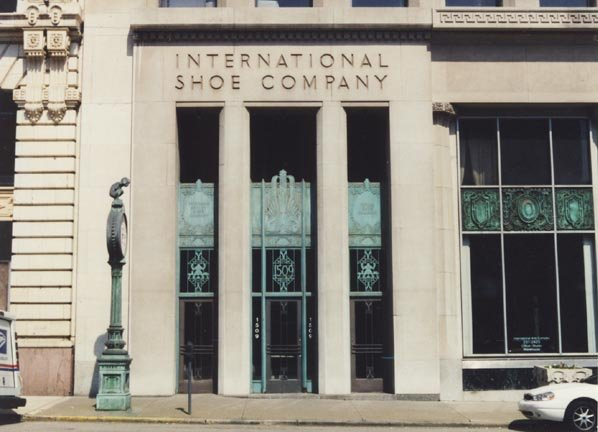
\includegraphics[width=0.33\linewidth,height=\textheight,keepaspectratio]{../img/IntlShoeBldg2.jpg}

}

\caption{International Shoe Co.~building, St.~Louis}

\end{figure}%

\emph{International Shoe} extended the reach of personal jurisdiction
over out-of-state parties. As a result, the exercise of jurisdiction no
longer requires personal service on the defendant while they are present
in the state.

Service of the complaint and summons is still required to satisfy the
notice aspect of due process. However, the Federal Rules of Civil
Procedure (adopted in 1938) relaxed that requirement, permitting service
by various alternate means and giving defendants an incentive to waive
formal service if they receive actual notice.
\href{https://www.law.cornell.edu/rules/frcp/rule_4}{Fed.R.Civ.P. Rule
4}.

The requirements of personal jurisdiction and service of process are
analogous to an electrical circuit. Minimum contacts between the
defendant and the forum state are the wiring. Service of process is the
switch. The court cannot exercise power over the defendant unless the
wiring is connected (personal jurisdiction) and the switch is turned on
(service of process).

Suppose that Dan, who lives in Ohio, rents a beach house in the Outer
Banks from Pat, who lives in North Carolina. One evening, while enjoying
several cocktails on the deck, Dan carelessly knocks over a Tiki torch,
setting fire to the house. After Dan returns home to Ohio, Pat files
suit in the U.S. District Court for the Eastern District of North
Carolina.

The suit arises out of Dan's conduct in North Carolina, satisfying the
minimum contacts requirement for personal jurisdiction. But there has
been no service of process, so the court's power is not yet activated.

\begin{figure}[H]

{\centering 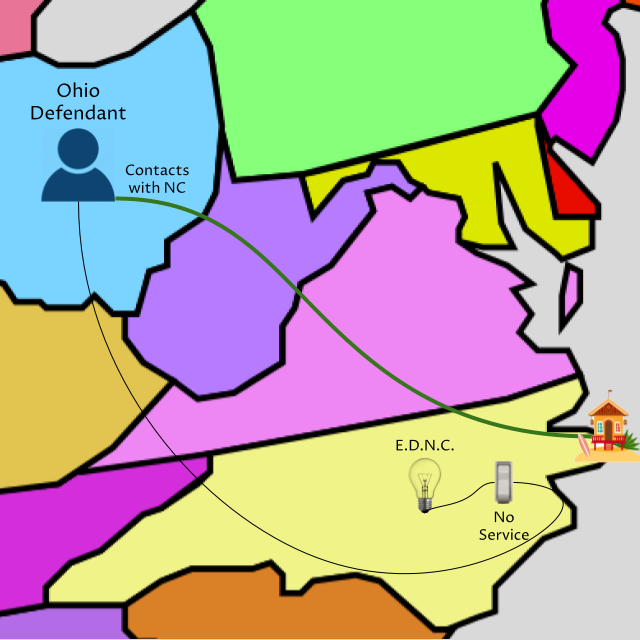
\includegraphics[width=0.33\linewidth,height=\textheight,keepaspectratio]{../img/PJ-NoService.png}

}

\caption{Pat v. Dan: Jurisdiction, No Service}

\end{figure}%

After filing the suit, Pat serves Dan with a copy of the summons and
complaint, in a manner authorized, and within the time allowed, under
Rule 4. The court's power is now active.

\begin{figure}[H]

{\centering 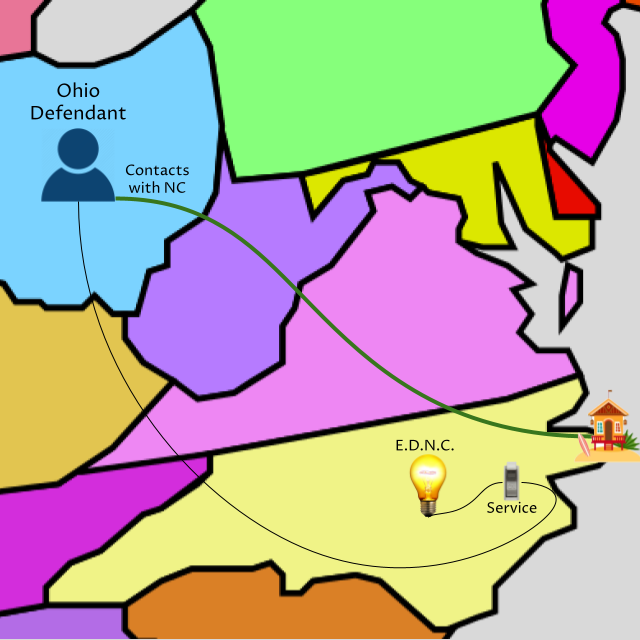
\includegraphics[width=0.33\linewidth,height=\textheight,keepaspectratio]{../img/PJ-Service.png}

}

\caption{Pat v. Dan: Jurisdiction \& Service}

\end{figure}%

Suppose instead that Pat travels from North Carolina to Ohio for a
football game between the Carolina Panthers and the Cleveland Browns.
Dan, a diehard Browns fan, was sitting behind Pat. Throughout the game,
Pat vociferously cheers for the visiting team and mercilessly heckles
the Cleveland quarterback. Annoyed with Pat's taunts, Dan pours a large
cup of beer over Pat's head, provoking a brawl in which Pat is badly
injured. After returning home, having vowed never to return to Ohio
again, Pat sues Dan for battery, filing the case in the U.S. District
Court for the Eastern District of North Carolina.

In this case, the suit does not arise out of any contacts between Dan
and North Carolina. Even Dan is served with a copy of the summons and
complaint, flipping the service switch has no effect, because the court
has no power over Dan at all.

\begin{figure}[H]

{\centering 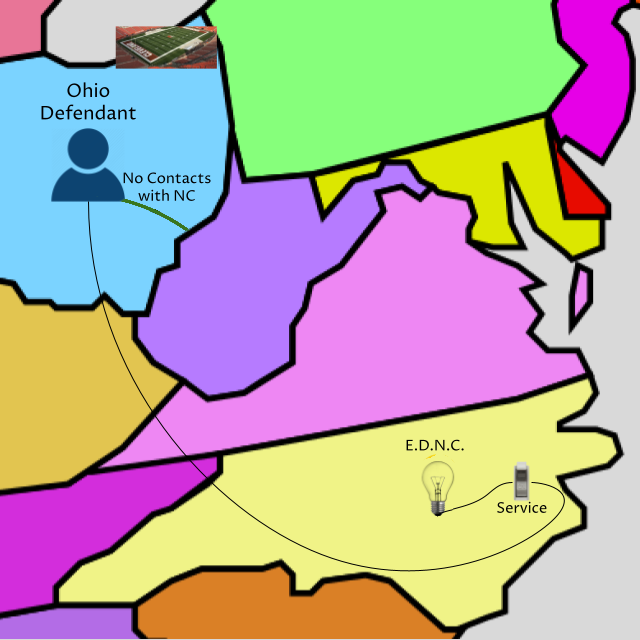
\includegraphics[width=0.33\linewidth,height=\textheight,keepaspectratio]{../img/NoPJ-Service.png}

}

\caption{Pat v. Dan: Service, No Jurisdiction}

\end{figure}%

\section{Specific Jurisdiction}\label{specific-jurisdiction}

\subsection{McGee v. International Life Ins. Co.~(U.S.
1957)}\label{mcgee-v.-international-life-ins.-co.-u.s.-1957}

\subsubsection{Opinion of the Court by Justice BLACK, announced by
Justice
DOUGLAS.}\label{opinion-of-the-court-by-justice-black-announced-by-justice-douglas.}

Petitioner, Lulu B. McGee, recovered a judgment in a California state
court against respondent, International Life Insurance Company, on a
contract of insurance. Respondent was not served with process in
California but by registered mail at its principal place of business in
Texas. The California court based its jurisdiction on a state statute
which subjects foreign corporations to suit in California on insurance
contracts with residents of that State even though such corporations
cannot be served with process within its borders.

Unable to collect the judgment in California petitioner went to Texas
where she filed suit on the judgment in a Texas court. But the Texas
courts refused to enforce her judgment holding it was void under the
Fourteenth Amendment because service of process outside California could
not give the courts of that State jurisdiction over respondent. Since
the case raised important questions, not only to California but to other
States which have similar laws, we granted certiorari. It is not
controverted that if the California court properly exercised
jurisdiction over respondent the Texas courts erred in refusing to give
its judgment full faith and credit.

The material facts are relatively simple. In 1944, Lowell Franklin, a
resident of California, purchased a life insurance policy from the
Empire Mutual Insurance Company, an Arizona corporation. In 1948 the
respondent agreed with Empire Mutual to assume its insurance
obligations. Respondent then mailed a reinsurance certificate to
Franklin in California offering to insure him in accordance with the
terms of the policy he held with Empire Mutual. He accepted this offer
and from that time until his death in 1950 paid premiums by mail from
his California home to respondent's Texas office. Petitioner, Franklin's
mother, was the beneficiary under the policy. She sent proofs of his
death to the respondent but it refused to pay claiming that he had
committed suicide. It appears that neither Empire Mutual nor respondent
has ever had any office or agent in California. And so far as the record
before us shows, respondent has never solicited or done any insurance
business in California apart from the policy involved here.

Since \emph{Pennoyer v. Neff}, this Court has held that the Due Process
Clause of the Fourteenth Amendment places some limit on the power of
state courts to enter binding judgments against persons not served with
process within their boundaries. But just where this line of limitation
falls has been the subject of prolific controversy, particularly with
respect to foreign corporations. In a continuing process of evolution
this Court accepted and then abandoned ``consent,'' ``doing business,''
and ``presence'' as the standard for measuring the extent of state
judicial power over such corporations. More recently in
\emph{International Shoe Co.~v. Washington}, the Court decided that
``due process requires only that in order to subject a defendant to a
judgment \emph{in personam,} if he be not present within the territory
of the forum, he have certain minimum contacts with it such that the
maintenance of the suit does not offend `traditional notions of fair
play and substantial justice.'\,''

Looking back over this long history of litigation a trend is clearly
discernible toward expanding the permissible scope of state jurisdiction
over foreign corporations and other nonresidents. In part this is
attributable to the fundamental transformation of our national economy
over the years. Today many commercial transactions touch two or more
States and may involve parties separated by the full continent. With
this increasing nationalization of commerce has come a great increase in
the amount of business conducted by mail across state lines. At the same
time modern transportation and communication have made it much less
burdensome for a party sued to defend himself in a State where he
engages in economic activity.

Turning to this case we think it apparent that the Due Process Clause
did not preclude the California court from entering a judgment binding
on respondent. It is sufficient for purposes of due process that the
suit was based on a contract which had substantial connection with that
State. The contract was delivered in California, the premiums were
mailed from there and the insured was a resident of that State when he
died. It cannot be denied that California has a manifest interest in
providing effective means of redress for its residents when their
insurers refuse to pay claims. These residents would be at a severe
disadvantage if they were forced to follow the insurance company to a
distant State in order to hold it legally accountable. When claims were
small or moderate individual claimants frequently could not afford the
cost of bringing an action in a foreign forum--- thus in effect making
the company judgment proof. Often the crucial witnesses---as here on the
company's defense of suicide---will be found in the insured's locality.
Of course there may be inconvenience to the insurer if it is held
amenable to suit in California where it had this contract but certainly
nothing which amounts to a denial of due process. There is no contention
that respondent did not have adequate notice of the suit or sufficient
time to prepare its defenses and appear.

The California statute became law in 1949, after respondent had entered
into the agreement with Franklin to assume Empire Mutual's obligation to
him. Respondent contends that application of the statute to this
existing contract improperly impairs the obligation of the contract. We
believe that contention is devoid of merit. The statute was remedial, in
the purest sense of that term, and neither enlarged nor impaired
respondent's substantive rights or obligations under the contract. It
did nothing more than to provide petitioner with a California forum to
enforce whatever substantive rights she might have against respondent.
At the same time respondent was given a reasonable time to appear and
defend on the merits after being notified of the suit. Under such
circumstances it had no vested right not to be sued in California.

The judgment is reversed and the cause is remanded to the Court of Civil
Appeals of the State of Texas, First Supreme Judicial District, for
further proceedings not inconsistent with this opinion.

\subsection{World-Wide Volkswagen Corp.~v. Woodson (U.S.
1979)}\label{world-wide-volkswagen-corp.-v.-woodson-u.s.-1979}

\subsubsection{Justice White delivered the opinion of the
Court.}\label{justice-white-delivered-the-opinion-of-the-court.}

The issue before us is whether, consistently with the Due Process Clause
of the Fourteenth Amendment, an Oklahoma court may exercise \emph{in
personam} jurisdiction over a nonresident automobile retailer and its
wholesale distributor in a products-liability action, when the
defendants' only connection with Oklahoma is the fact that an automobile
sold in New York to New York residents became involved in an accident in
Oklahoma.

\subsubsection{I}\label{i}

Respondents Harry and Kay Robinson purchased a new Audi automobile from
petitioner Seaway Volkswagen, Inc.~(Seaway), in Massena, N. Y., in 1976.
The following year the Robinson family, who resided in New York, left
that State for a new home in Arizona. As they passed through the State
of Oklahoma, another car struck their Audi in the rear, causing a fire
which severely burned Kay Robinson and her two children.

The Robinsons subsequently brought a products-liability action in the
District Court for Creek County, Okla., claiming that their injuries
resulted from defective design and placement of the Audi's gas tank and
fuel system. They joined as defendants the automobile's manufacturer,
Audi NSU Auto Union Aktiengesellschaft (Audi); its importer, Volkswagen
of America, Inc.~(Volkswagen); its regional distributor, petitioner
World-Wide Volkswagen Corp.~(World-Wide); and its retail dealer,
petitioner Seaway. Seaway and World-Wide entered special appearances,
claiming that Oklahoma's exercise of jurisdiction over them would offend
the limitations on the State's jurisdiction imposed by the Due Process
Clause of the Fourteenth Amendment.

The facts presented to the District Court showed that World-Wide is
incorporated and has its business office in New York. It distributes
vehicles, parts, and accessories, under contract with Volkswagen, to
retail dealers in New York, New Jersey, and Connecticut. Seaway, one of
these retail dealers, is incorporated and has its place of business in
New York. Insofar as the record reveals, Seaway and World-Wide are fully
independent corporations whose relations with each other and with
Volkswagen and Audi are contractual only. Respondents adduced no
evidence that either World-Wide or Seaway does any business in Oklahoma,
ships or sells any products to or in that State, has an agent to receive
process there, or purchases advertisements in any media calculated to
reach Oklahoma. In fact, as respondents' counsel conceded at oral
argument, there was no showing that any automobile sold by World-Wide or
Seaway has ever entered Oklahoma with the single exception of the
vehicle involved in the present case.

\subsubsection{II}\label{ii}

The Due Process Clause of the Fourteenth Amendment limits the power of a
state court to render a valid personal judgment against a nonresident
defendant. A judgment rendered in violation of due process is void in
the rendering State and is not entitled to full faith and credit
elsewhere. Due process requires that the defendant be given adequate
notice of the suit, and be subject to the personal jurisdiction of the
court, In the present case, the only question is whether these
particular petitioners were subject to the jurisdiction of the Oklahoma
courts.

As has long been settled, and as we reaffirm today, a state court may
exercise personal jurisdiction over a nonresident defendant only so long
as there exist ``minimum contacts'' between the defendant and the forum
State. \emph{International Shoe Co.~v. Washington}. The concept of
minimum contacts, in turn, can be seen to perform two related, but
distinguishable, functions. It protects the defendant against the
burdens of litigating in a distant or inconvenient forum. And it acts to
ensure that the States, through their courts, do not reach out beyond
the limits imposed on them by their status as coequal sovereigns in a
federal system.

The protection against inconvenient litigation is typically described in
terms of ``reasonableness'' or ``fairness.'' We have said that the
defendant's contacts with the forum State must be such that maintenance
of the suit ``does not offend `traditional notions of fair play and
substantial justice.'\,'' \emph{International Shoe Co.} The relationship
between the defendant and the forum must be such that it is ``reasonable
to require the corporation to defend the particular suit which is
brought there.'' Implicit in this emphasis on reasonableness is the
understanding that the burden on the defendant, while always a primary
concern, will in an appropriate case be considered in light of other
relevant factors, including the forum State's interest in adjudicating
the dispute, the plaintiff's interest in obtaining convenient and
effective relief, at least when that interest is not adequately
protected by the plaintiff's power to choose the forum, the interstate
judicial system's interest in obtaining the most efficient resolution of
controversies; and the shared interest of the several States in
furthering fundamental substantive social policies.

The limits imposed on state jurisdiction by the Due Process Clause, in
its role as a guarantor against inconvenient litigation, have been
substantially relaxed over the years. As we noted in \emph{McGee v.
International Life Ins. Co.,} this trend is largely attributable to a
fundamental transformation in the American economy:

\begin{quote}
Today many commercial transactions touch two or more States and may
involve parties separated by the full continent. With this increasing
nationalization of commerce has come a great increase in the amount of
business conducted by mail across state lines. At the same time modern
transportation and communication have made it much less burdensome for a
party sued to defend himself in a State where he engages in economic
activity.
\end{quote}

The historical developments noted in \emph{McGee,} of course, have only
accelerated in the generation since that case was decided.

Nevertheless, we have never accepted the proposition that state lines
are irrelevant for jurisdictional purposes, nor could we, and remain
faithful to the principles of interstate federalism embodied in the
Constitution. The economic interdependence of the States was foreseen
and desired by the Framers. In the Commerce Clause, they provided that
the Nation was to be a common market, a ``free trade unit'' in which the
States are debarred from acting as separable economic entities. But the
Framers also intended that the States retain many essential attributes
of sovereignty, including, in particular, the sovereign power to try
causes in their courts. The sovereignty of each State, in turn, implied
a limitation on the sovereignty of all of its sister States---a
limitation express or implicit in both the original scheme of the
Constitution and the Fourteenth Amendment.

Hence, even while abandoning the shibboleth that ``the authority of
every tribunal is necessarily restricted by the territorial limits of
the State in which it is established,'' \emph{Pennoyer v. Neff,} we
emphasized that the reasonableness of asserting jurisdiction over the
defendant must be assessed ``in the context of our federal system of
government,'' \emph{International Shoe Co.~v. Washington,} and stressed
that the Due Process Clause ensures not only fairness, but also the
``orderly administration of the laws,'' \emph{id.} As we noted in
\emph{Hanson v. Denckla,} 357 U. S. 235, 250-251 (1958):

\begin{quote}
As technological progress has increased the flow of commerce between the
States, the need for jurisdiction over nonresidents has undergone a
similar increase. At the same time, progress in communications and
transportation has made the defense of a suit in a foreign tribunal less
burdensome. In response to these changes, the requirements for personal
jurisdiction over nonresidents have evolved from the rigid rule of
\emph{Pennoyer v. Neff} to the flexible standard of \emph{International
Shoe Co.~v. Washington}. But it is a mistake to assume that this trend
heralds the eventual demise of all restrictions on the personal
jurisdiction of state courts. Those restrictions are more than a
guarantee of immunity from inconvenient or distant litigation. They are
a consequence of territorial limitations on the power of the respective
States.
\end{quote}

Thus, the Due Process Clause ``does not contemplate that a state may
make binding a judgment \emph{in personam} against an individual or
corporate defendant with which the state has no contacts, ties, or
relations.'' \emph{International Shoe Co.} Even if the defendant would
suffer minimal or no inconvenience from being forced to litigate before
the tribunals of another State; even if the forum State has a strong
interest in applying its law to the controversy; even if the forum State
is the most convenient location for litigation, the Due Process Clause,
acting as an instrument of interstate federalism, may sometimes act to
divest the State of its power to render a valid judgment.

\subsubsection{III}\label{iii}

Applying these principles to the case at hand, we find in the record
before us a total absence of those affiliating circumstances that are a
necessary predicate to any exercise of state-court jurisdiction.
Petitioners carry on no activity whatsoever in Oklahoma. They close no
sales and perform no services there. They avail themselves of none of
the privileges and benefits of Oklahoma law. They solicit no business
there either through salespersons or through advertising reasonably
calculated to reach the State. Nor does the record show that they
regularly sell cars at wholesale or retail to Oklahoma customers or
residents or that they indirectly, through others, serve or seek to
serve the Oklahoma market. In short, respondents seek to base
jurisdiction on one, isolated occurrence and whatever inferences can be
drawn therefrom: the fortuitous circumstance that a single Audi
automobile, sold in New York to New York residents, happened to suffer
an accident while passing through Oklahoma.

It is argued, however, that because an automobile is mobile by its very
design and purpose it was ``foreseeable'' that the Robinsons' Audi would
cause injury in Oklahoma. Yet ``foreseeability'' alone has never been a
sufficient benchmark for personal jurisdiction under the Due Process
Clause.

This is not to say, of course, that foreseeability is wholly irrelevant.
But the foreseeability that is critical to due process analysis is not
the mere likelihood that a product will find its way into the forum
State. Rather, it is that the defendant's conduct and connection with
the forum State are such that he should reasonably anticipate being
haled into court there. The Due Process Clause, by ensuring the
``orderly administration of the laws,'' \emph{International Shoe Co.,}
gives a degree of predictability to the legal system that allows
potential defendants to structure their primary conduct with some
minimum assurance as to where that conduct will and will not render them
liable to suit.

When a corporation ``purposefully avails itself of the privilege of
conducting activities within the forum State,'' \emph{Hanson v.
Denckla,} it has clear notice that it is subject to suit there, and can
act to alleviate the risk of burdensome litigation by procuring
insurance, passing the expected costs on to customers, or, if the risks
are too great, severing its connection with the State. Hence if the sale
of a product of a manufacturer or distributor such as Audi or Volkswagen
is not simply an isolated occurrence, but arises from the efforts of the
manufacturer or distributor to serve, directly or indirectly, the market
for its product in other States, it is not unreasonable to subject it to
suit in one of those States if its allegedly defective merchandise has
there been the source of injury to its owner or to others. The forum
State does not exceed its powers under the Due Process Clause if it
asserts personal jurisdiction over a corporation that delivers its
products into the stream of commerce with the expectation that they will
be purchased by consumers in the forum State.

But there is no such or similar basis for Oklahoma jurisdiction over
World-Wide or Seaway in this case. Seaway's sales are made in Massena,
N. Y. World-Wide's market, although substantially larger, is limited to
dealers in New York, New Jersey, and Connecticut. There is no evidence
of record that any automobiles distributed by World-Wide are sold to
retail customers outside this tristate area. It is foreseeable that the
purchasers of automobiles sold by World-Wide and Seaway may take them to
Oklahoma. But the mere ``unilateral activity of those who claim some
relationship with a nonresident defendant cannot satisfy the requirement
of contact with the forum State.'' \emph{Hanson v. Denckla}.

In a variant on the previous argument, it is contended that jurisdiction
can be supported by the fact that petitioners earn substantial revenue
from goods used in Oklahoma. While this inference seems less than
compelling on the facts of the instant case, we need not question the
court's factual findings in order to reject its reasoning.

This argument seems to make the point that the purchase of automobiles
in New York, from which the petitioners earn substantial revenue, would
not occur \emph{but for} the fact that the automobiles are capable of
use in distant States like Oklahoma. Respondents observe that the very
purpose of an automobile is to travel, and that travel of automobiles
sold by petitioners is facilitated by an extensive chain of Volkswagen
service centers throughout the country, including some in Oklahoma.
However, financial benefits accruing to the defendant from a collateral
relation to the forum State will not support jurisdiction if they do not
stem from a constitutionally cognizable contact with that State. In our
view, whatever marginal revenues petitioners may receive by virtue of
the fact that their products are capable of use in Oklahoma is far too
attenuated a contact to justify that State's exercise of \emph{in
personam} jurisdiction over them.

\subsubsection{Justice Brennan,
dissenting.}\label{justice-brennan-dissenting.}

The Court holds that the Due Process Clause of the Fourteenth Amendment
bars the States from asserting jurisdiction over the defendants in these
two cases. In each case the Court so decides because it fails to find
the ``minimum contacts'' that have been required since
\emph{International Shoe Co.~v. Washington}. Because I believe that the
Court reads \emph{International Shoe} and its progeny too narrowly, and
because I believe that the standards enunciated by those cases may
already be obsolete as constitutional boundaries, I dissent.

\subsubsection{I}\label{i-1}

The Court's opinions focus tightly on the existence of contacts between
the forum and the defendant. In so doing, they accord too little weight
to the strength of the forum State's interest in the case and fail to
explore whether there would be any actual inconvenience to the
defendant. The essential inquiry in locating the constitutional limits
on state-court jurisdiction over absent defendants is whether the
particular exercise of jurisdiction offends ``\,`traditional notions of
fair play and substantial justice.'\,'' \emph{International Shoe}. The
clear focus in \emph{International Shoe} was on fairness and
reasonableness. The Court specifically declined to establish a
mechanical test based on the quantum of contacts between a State and the
defendant:

\begin{quote}
Whether due process is satisfied must depend rather upon the quality and
nature of the activity \emph{in relation to the fair and orderly
administration of the laws which it was the purpose of the due process
clause to insure.} That clause does not contemplate that a state may
make binding a judgment \emph{in personam} against an individual or
corporate defendant with which the state has \emph{no} contacts, ties,
or relations.
\end{quote}

The existence of contacts, so long as there were some, was merely one
way of giving content to the determination of fairness and
reasonableness.

Surely \emph{International Shoe} contemplated that the significance of
the contacts necessary to support jurisdiction would diminish if some
other consideration helped establish that jurisdiction would be fair and
reasonable. The interests of the State and other parties in proceeding
with the case in a particular forum are such considerations. \emph{McGee
v. International Life Ins. Co.}, for instance, accorded great importance
to a State's ``manifest interest in providing effective means of
redress'' for its citizens.

Another consideration is the actual burden a defendant must bear in
defending the suit in the forum. Because lesser burdens reduce the
unfairness to the defendant, jurisdiction may be justified despite less
significant contacts. The burden, of course, must be of constitutional
dimension. Due process limits on jurisdiction do not protect a defendant
from all inconvenience of travel, and it would not be sensible to make
the constitutional rule turn solely on the number of miles the defendant
must travel to the courtroom. Instead, the constitutionally significant
``burden'' to be analyzed relates to the mobility of the defendant's
defense. For instance, if having to travel to a foreign forum would
hamper the defense because witnesses or evidence or the defendant
himself were immobile, or if there were a disproportionately large
number of witnesses or amount of evidence that would have to be
transported at the defendant's expense, or if being away from home for
the duration of the trial would work some special hardship on the
defendant, then the Constitution would require special consideration for
the defendant's interests.

That considerations other than contacts between the forum and the
defendant are relevant necessarily means that the Constitution does not
require that trial be held in the State which has the ``best contacts''
with the defendant.The defendant has no constitutional entitlement to
the best forum or, for that matter, to any particular forum. We need
only determine whether the forum States in these cases satisfy the
constitutional minimum.

\subsubsection{II}\label{ii-1}

I would find that the forum State has an interest in permitting the
litigation to go forward, the litigation is connected to the forum, the
defendant is linked to the forum, and the burden of defending is not
unreasonable. Accordingly, I would hold that it is neither unfair nor
unreasonable to require these defendants to defend in the forum State.

The interest of the forum State and its connection to the litigation is
strong. The automobile accident underlying the litigation occurred in
Oklahoma. The plaintiffs were hospitalized in Oklahoma when they brought
suit. Essential witnesses and evidence were in Oklahoma. The State has a
legitimate interest in enforcing its laws designed to keep its highway
system safe, and the trial can proceed at least as efficiently in
Oklahoma as anywhere else.

The petitioners are not unconnected with the forum. Although both sell
automobiles within limited sales territories, each sold the automobile
which in fact was driven to Oklahoma where it was involved in an
accident. It may be true, as the Court suggests, that each sincerely
intended to limit its commercial impact to the limited territory, and
that each intended to accept the benefits and protection of the laws
only of those States within the territory. But obviously these were
unrealistic hopes that cannot be treated as an automatic constitutional
shield.

An automobile simply is not a stationary item or one designed to be used
in one place. An automobile is \emph{intended} to be moved around.
Someone in the business of selling large numbers of automobiles can
hardly plead ignorance of their mobility or pretend that the automobiles
stay put after they are sold. It is not merely that a dealer in
automobiles foresees that they will move. The dealer actually intends
that the purchasers will use the automobiles to travel to distant States
where the dealer does not directly ``do business.'' The sale of an
automobile does \emph{purposefully} inject the vehicle into the stream
of interstate commerce so that it can travel to distant States.

Furthermore, an automobile seller derives substantial benefits from
States other than its own. A large part of the value of automobiles is
the extensive, nationwide network of highways. Significant portions of
that network have been constructed by and are maintained by the
individual States, including Oklahoma. The States, through their highway
programs, contribute in a very direct and important way to the value of
petitioners' businesses. Additionally, a network of other related
dealerships with their service departments operates throughout the
country under the protection of the laws of the various States,
including Oklahoma, and enhances the value of petitioners' businesses by
facilitating their customers' traveling.

Thus, the Court errs in its conclusion that ``petitioners have \emph{no}
contacts, ties, or relations''' with Oklahoma. There obviously are
contacts, and, given Oklahoma's connection to the litigation, the
contacts are sufficiently significant to make it fair and reasonable for
the petitioners to submit to Oklahoma's jurisdiction.

\subsubsection{III}\label{iii-1}

\emph{International Shoe} inherited its defendant focus from
\emph{Pennoyer v. Neff,} and represented the last major step this Court
has taken in the long process of liberalizing the doctrine of personal
jurisdiction. Though its flexible approach represented a major advance,
the structure of our society has changed in many significant ways since
\emph{International Shoe} was decided in 1945. Mr.~Justice Black,
writing for the Court in \emph{McGee}, recognized that ``a trend is
clearly discernible toward expanding the permissible scope of state
jurisdiction over foreign corporations and other nonresidents.'' He
explained the trend as follows:

\begin{quote}
In part this is attributable to the fundamental transformation of our
national economy over the years. Today many commercial transactions
touch two or more States and may involve parties separated by the full
continent. With this increasing nationalization of commerce has come a
great increase in the amount of business conducted by mail across state
lines. At the same time modern transportation and communication have
made it much less burdensome for a party sued to defend himself in a
State where he engages in economic activity.
\end{quote}

Both the nationalization of commerce and the ease of transportation and
communication have accelerated in the generation since 1957. The model
of society on which the \emph{International Shoe} Court based its
opinion is no longer accurate. Business people, no matter how local
their businesses, cannot assume that goods remain in the business'
locality. Customers and goods can be anywhere else in the country
usually in a matter of hours and always in a matter of a very few days.

In answering the question whether or not it is fair and reasonable to
allow a particular forum to hold a trial binding on a particular
defendant, the interests of the forum State and other parties loom large
in today's world and surely are entitled to as much weight as are the
interests of the defendant. The ``orderly administration of the laws''
provides a firm basis for according some protection to the interests of
plaintiffs and States as well as of defendants. Certainly, I cannot see
how a defendant's right to due process is violated if the defendant
suffers no inconvenience.

The conclusion I draw is that constitutional concepts of fairness no
longer require the extreme concern for defendants that was once
necessary. Rather, minimum contacts must exist ``among the
\emph{parties,} the contested transaction, and the forum State.'' The
contacts between any two of these should not be determinate.

\textbf{Justice BLACKMUN, dissenting.}

I confess that I am somewhat puzzled why the plaintiffs in this
litigation are so insistent that the regional distributor and the retail
dealer, the petitioners here, who handled the ill-fated Audi automobile
involved in this litigation, be named defendants. It would appear that
the manufacturer and the importer, whose subjectability to Oklahoma
jurisdiction is not challenged before this Court, ought not to be
judgment-proof. It may, of course, ultimately amount to a contest
between insurance companies that, once begun, is not easily brought to a
termination. Having made this much of an observation, I pursue it no
further.

\subsection{Ford Motor Co.~v. Montana Eighth Judicial Dist. Court (U.S.
2021)}\label{ford-motor-co.-v.-montana-eighth-judicial-dist.-court-u.s.-2021}

\textbf{Justice KAGAN delivered the opinion of the Court.}

In each of these two cases, a state court held that it had jurisdiction
over Ford Motor Company in a products-liability suit stemming from a car
accident. The accident happened in the State where suit was brought. The
victim was one of the State's residents. And Ford did substantial
business in the State---among other things, advertising, selling, and
servicing the model of vehicle the suit claims is defective. Still, Ford
contends that jurisdiction is improper because the particular car
involved in the crash was not first sold in the forum State, nor was it
designed or manufactured there. We reject that argument. When a company
like Ford serves a market for a product in a State and that product
causes injury in the State to one of its residents, the State's courts
may entertain the resulting suit.

\subsubsection{I}\label{i-2}

Ford is a global auto company. It is incorporated in Delaware and
headquartered in Michigan. But its business is everywhere. Ford markets,
sells, and services its products across the United States and overseas.
In this country alone, the company annually distributes over 2.5 million
new cars, trucks, and SUVs to over 3,200 licensed dealerships. Ford also
encourages a resale market for its products: Almost all its dealerships
buy and sell used Fords, as well as selling new ones. To enhance its
brand and increase its sales, Ford engages in wide-ranging promotional
activities, including television, print, online, and direct-mail
advertisements. No matter where you live, you've seen them: ``Have you
driven a Ford lately?'' or ``Built Ford Tough.'' Ford also ensures that
consumers can keep their vehicles running long past the date of sale.
The company provides original parts to auto supply stores and repair
shops across the country. (Goes another slogan: ``Keep your Ford a
Ford.'') And Ford's own network of dealers offers an array of
maintenance and repair services, thus fostering an ongoing relationship
between Ford and its customers.

Accidents involving two of Ford's vehicles---a 1996 Explorer and a 1994
Crown Victoria---are at the heart of the suits before us. One case comes
from Montana. Markkaya Gullett was driving her Explorer near her home in
the State when the tread separated from a rear tire. The vehicle spun
out, rolled into a ditch, and came to rest upside down. Gullett died at
the scene of the crash. The representative of her estate sued Ford in
Montana state court, bringing claims for a design defect, failure to
warn, and negligence. The second case comes from Minnesota. Adam
Bandemer was a passenger in his friend's Crown Victoria, traveling on a
rural road in the State to a favorite ice-fishing spot. When his friend
rear-ended a snowplow, this car too landed in a ditch. Bandemer's air
bag failed to deploy, and he suffered serious brain damage. He sued Ford
in Minnesota state court, asserting products-liability, negligence, and
breach-of-warranty claims.

Ford moved to dismiss the two suits for lack of personal jurisdiction,
on basically identical grounds. According to Ford, the state court
(whether in Montana or Minnesota) had jurisdiction only if the company's
conduct in the State had given rise to the plaintiff's claims. And that
causal link existed, Ford continued, only if the company had designed,
manufactured, or---most likely---sold in the State the particular
vehicle involved in the accident. In neither suit could the plaintiff
make that showing. Ford had designed the Explorer and Crown Victoria in
Michigan, and it had manufactured the cars in (respectively) Kentucky
and Canada. Still more, the company had originally sold the cars at
issue outside the forum States---the Explorer in Washington, the Crown
Victoria in North Dakota. Only later resales and relocations by
consumers had brought the vehicles to Montana and Minnesota. That meant,
in Ford's view, that the courts of those States could not decide the
suits.

Both the Montana and the Minnesota Supreme Courts (affirming lower court
decisions) rejected Ford's argument.

We granted certiorari to consider if Ford is subject to jurisdiction in
these cases. We hold that it is.

\subsubsection{II}\label{ii-2}

The Fourteenth Amendment's Due Process Clause limits a state court's
power to exercise jurisdiction over a defendant. The canonical decision
in this area remains \emph{International Shoe Co.~v. Washington}. There,
the Court held that a tribunal's authority depends on the defendant's
having such ``contacts'' with the forum State that ``the maintenance of
the suit'' is ``reasonable, in the context of our federal system of
government,'' and ``does not offend traditional notions of fair play and
substantial justice.'' In giving content to that formulation, the Court
has long focused on the nature and extent of ``the defendant's
relationship to the forum State.'' That focus led to our recognizing two
kinds of personal jurisdiction: general (sometimes called all-purpose)
jurisdiction and specific (sometimes called case-linked) jurisdiction.

A state court may exercise general jurisdiction only when a defendant is
``essentially at home'' in the State. General jurisdiction, as its name
implies, extends to ``any and all claims'' brought against a defendant.
Those claims need not relate to the forum State or the defendant's
activity there; they may concern events and conduct anywhere in the
world. But that breadth imposes a correlative limit: Only a select ``set
of affiliations with a forum'' will expose a defendant to such sweeping
jurisdiction. what we have called the ``paradigm'' case, an individual
is subject to general jurisdiction in her place of domicile. And the
``equivalent'' forums for a corporation are its place of incorporation
and principal place of business. So general jurisdiction over Ford (as
all parties agree) attaches in Delaware and Michigan---not in Montana
and Minnesota.

Specific jurisdiction is different: It covers defendants less intimately
connected with a State, but only as to a narrower class of claims. The
contacts needed for this kind of jurisdiction often go by the name
``purposeful availment.'' The defendant, we have said, must take ``some
act by which it purposefully avails itself of the privilege of
conducting activities within the forum State.'' The contacts must be the
defendant's own choice and not ``random, isolated, or fortuitous.'' They
must show that the defendant deliberately ``reached out beyond'' its
home---by, for example, ``exploiting a market'' in the forum State or
entering a contractual relationship centered there. Yet even
then---because the defendant is not ``at home''---the forum State may
exercise jurisdiction in only certain cases. The plaintiff's claims, we
have often stated, ``must arise out of or relate to the defendant's
contacts'' with the forum. Or put just a bit differently, ``there must
be `an affiliation between the forum and the underlying controversy,
principally, an activity or an occurrence that takes place in the forum
State and is therefore subject to the State's regulation.'\,''

These rules derive from and reflect two sets of values---treating
defendants fairly and protecting ``interstate federalism.'' Our decision
in \emph{International Shoe} founded specific jurisdiction on an idea of
reciprocity between a defendant and a State: When (but only when) a
company ``exercises the privilege of conducting activities within a
state''---thus ``enjoying the benefits and protection of its
laws''---the State may hold the company to account for related
misconduct. Later decisions have added that our doctrine similarly
provides defendants with ``fair warning''---knowledge that ``a
particular activity may subject it to the jurisdiction of a foreign
sovereign.'' A defendant can thus ``structure its primary conduct'' to
lessen or avoid exposure to a given State's courts. And this Court has
considered alongside defendants' interests those of the States in
relation to each other. One State's ``sovereign power to try'' a suit,
we have recognized, may prevent ``sister States'' from exercising their
like authority. The law of specific jurisdiction thus seeks to ensure
that States with ``little legitimate interest'' in a suit do not
encroach on States more affected by the controversy.

Ford contends that our jurisdictional rules prevent Montana's and
Minnesota's courts from deciding these two suits. In making that
argument, Ford does not contest that it does substantial business in
Montana and Minnesota---that it actively seeks to serve the market for
automobiles and related products in those States. Or to put that
concession in more doctrinal terms, Ford agrees that it has
``purposefully availed itself of the privilege of conducting
activities'' in both places. Ford's claim is instead that those
activities do not sufficiently connect to the suits, even though the
resident-plaintiffs allege that Ford cars malfunctioned in the forum
States. In Ford's view, the needed link must be causal in nature:
Jurisdiction attaches ``only if the defendant's forum conduct \emph{gave
rise} to the plaintiff's claims.'' And that rule reduces, Ford thinks,
to locating specific jurisdiction in the State where Ford sold the car
in question, or else the States where Ford designed and manufactured the
vehicle. On that view, the place of accident and injury is immaterial.
So (Ford says) Montana's and Minnesota's courts have no power over these
cases.

But Ford's causation-only approach finds no support in this Court's
requirement of a ``connection'' between a plaintiff's suit and a
defendant's activities. That rule indeed serves to narrow the class of
claims over which a state court may exercise specific jurisdiction. But
not quite so far as Ford wants. None of our precedents has suggested
that only a strict causal relationship between the defendant's in-state
activity and the litigation will do. As just noted, our most common
formulation of the rule demands that the suit ``arise out of \emph{or
relate to} the defendant's contacts with the forum.'' The first half of
that standard asks about causation; but the back half, after the ``or,''
contemplates that some relationships will support jurisdiction without a
causal showing. That does not mean anything goes. In the sphere of
specific jurisdiction, the phrase ``relate to'' incorporates real
limits, as it must to adequately protect defendants foreign to a forum.
But again, we have never framed the specific jurisdiction inquiry as
always requiring proof of causation---\emph{i.e.}, proof that the
plaintiff's claim came about because of the defendant's in-state
conduct. So the case is not over even if, as Ford argues, a causal test
would put jurisdiction in only the States of first sale, manufacture,
and design. A different State's courts may yet have jurisdiction,
because of another ``activity or occurrence'' involving the defendant
that takes place in the State.

And indeed, this Court has stated that specific jurisdiction attaches in
cases identical to the ones here---when a company like Ford serves a
market for a product in the forum State and the product malfunctions
there. In \emph{World-Wide Volkswagen}, the Court held that an Oklahoma
court could not assert jurisdiction over a New York car dealer just
because a car it sold later caught fire in Oklahoma. But in so doing, we
contrasted the dealer's position to that of two other defendants---Audi,
the car's manufacturer, and Volkswagen, the car's nationwide importer
(neither of which contested jurisdiction):

\begin{quote}
If the sale of a product of a manufacturer or distributor such as Audi
or Volkswagen is not simply an isolated occurrence, but arises from the
efforts of the manufacturer or distributor to serve, directly or
indirectly, the market for its product in several or all other States,
it is not unreasonable to subject it to suit in one of those States if
its allegedly defective merchandise has there been the source of injury
to its owner or to others.
\end{quote}

Or said another way, if Audi and Volkswagen's business deliberately
extended into Oklahoma (among other States), then Oklahoma's courts
could hold the companies accountable for a car's catching fire
there---even though the vehicle had been designed and made overseas and
sold in New York. For, the Court explained, a company thus
``purposefully availing itself''of the Oklahoma auto market ``has clear
notice'' of its exposure in that State to suits arising from local
accidents involving its cars. And the company could do something about
that exposure: It could ``act to alleviate the risk of burdensome
litigation by procuring insurance, passing the expected costs on to
customers, or, if the risks are still too great, severing its connection
with the State.''

Our conclusion in \emph{World-Wide Volkswagen}---though, as Ford notes,
technically ``dicta''---has appeared and reappeared in many cases since.
So, for example, the Court in \emph{Keeton} invoked that part of
\emph{World-Wide Volkswagen} to show that when a corporation has
``continuously and deliberately exploited a State's market, it must
reasonably anticipate being haled into that State's courts'' to defend
actions ``based on'' products causing injury there. And in
\emph{Daimler}, we used the Audi/Volkswagen scenario as a paradigm case
of specific jurisdiction (though now naming Daimler, the maker of
Mercedes Benzes). Said the Court, to ``illustrate'' specific
jurisdiction's ``province'': A California court would exercise specific
jurisdiction ``if a California plaintiff, injured in a California
accident involving a Daimler-manufactured vehicle, sued Daimler in that
court alleging that the vehicle was defectively designed.'' As in
\emph{World-Wide Volkswagen}, the Court did not limit jurisdiction to
where the car was designed, manufactured, or first sold. Substitute Ford
for Daimler, Montana and Minnesota for California, and the Court's
``illustrative'' case becomes \ldots{} the two cases before us.

To see why Ford is subject to jurisdiction in these cases (as Audi,
Volkswagen, and Daimler were in their analogues), consider first the
business that the company regularly conducts in Montana and Minnesota.
Small wonder that Ford has here conceded ``purposeful availment'' of the
two States' markets. By every means imaginable---among them, billboards,
TV and radio spots, print ads, and direct mail---Ford urges Montanans
and Minnesotans to buy its vehicles, including (at all relevant times)
Explorers and Crown Victorias. Ford cars---again including those two
models---are available for sale, whether new or used, throughout the
States, at 36 dealerships in Montana and 84 in Minnesota. And apart from
sales, Ford works hard to foster ongoing connections to its cars'
owners. The company's dealers in Montana and Minnesota (as elsewhere)
regularly maintain and repair Ford cars, including those whose
warranties have long since expired. And the company distributes
replacement parts both to its own dealers and to independent auto shops
in the two States. Those activities, too, make Ford money. And by making
it easier to own a Ford, they encourage Montanans and Minnesotans to
become lifelong Ford drivers.

Now turn to how all this Montana-and Minnesota-based conduct relates to
the claims in these cases, brought by state residents in Montana's and
Minnesota's courts. Each plaintiff's suit, of course, arises from a car
accident in one of those States. In each complaint, the
resident-plaintiff alleges that a defective Ford vehicle---an Explorer
in one, a Crown Victoria in the other---caused the crash and resulting
harm. And as just described, Ford had advertised, sold, and serviced
those two car models in both States for many years. (Contrast a case,
which we do not address, in which Ford marketed the models in only a
different State or region.) In other words, Ford had systematically
served a market in Montana and Minnesota for the very vehicles that the
plaintiffs allege malfunctioned and injured them in those States. So
there is a strong ``relationship among the defendant, the forum, and the
litigation''---the ``essential foundation'' of specific jurisdiction.
That is why this Court has used this exact fact pattern (a
resident-plaintiff sues a global car company, extensively serving the
state market in a vehicle, for an in-state accident) as an
illustration---even a paradigm example---of how specific jurisdiction
works.\footnote{(n.4 in opinion) None of this is to say that any person
  using any means to sell any good in a State is subject to jurisdiction
  there if the product malfunctions after arrival. We have long treated
  isolated or sporadic transactions differently from continuous ones.
  And we do not here consider Internet transactions, which may raise
  doctrinal questions of their own.}

The only complication here, pressed by Ford, is that the company sold
the specific cars involved in these crashes outside the forum States,
with consumers later selling them to the States' residents. Because that
is so, Ford argues, the plaintiffs' claims ``would be precisely the same
if Ford had never done anything in Montana and Minnesota.'' Of course,
that argument merely restates Ford's demand for an exclusively causal
test of connection---which we have already shown is inconsistent with
our caselaw. And indeed, a similar assertion could have been made in
\emph{World-Wide Volkswagen}---yet the Court made clear that systematic
contacts in Oklahoma rendered Audi accountable there for an in-state
accident, even though it involved a car sold in New York. So too here,
and for the same reasons---even supposing (as Ford does) that without
the company's Montana or Minnesota contacts the plaintiffs' claims would
be just the same.

But in any event, that assumption is far from clear. For the owners of
these cars might never have bought them, and so these suits might never
have arisen, except for Ford's contacts with their home States. Those
contacts might turn any resident of Montana or Minnesota into a Ford
owner---even when he buys his car from out of state. He may make that
purchase because he saw ads for the car in local media. And he may take
into account a raft of Ford's in-state activities designed to make
driving a Ford convenient there: that Ford dealers stand ready to
service the car; that other auto shops have ample supplies of Ford
parts; and that Ford fosters an active resale market for its old models.
The plaintiffs here did not in fact establish, or even allege, such
causal links. Nor should jurisdiction in cases like these ride on the
exact reasons for an individual plaintiff's purchase, or on his ability
to present persuasive evidence about them. But the possibilities listed
above---created by the reach of Ford's Montana and Minnesota
contacts---underscore the aptness of finding jurisdiction here, even
though the cars at issue were first sold out of state.

For related reasons, allowing jurisdiction in these cases treats Ford
fairly, as this Court's precedents explain. In conducting so much
business in Montana and Minnesota, Ford ``enjoys the benefits and
protection of their laws''---the enforcement of contracts, the defense
of property, the resulting formation of effective markets. All that
assistance to Ford's in-state business creates reciprocal
obligations---most relevant here, that the car models Ford so
extensively markets in Montana and Minnesota be safe for their citizens
to use there. Thus our repeated conclusion: A state court's enforcement
of that commitment, enmeshed as it is with Ford's government-protected
in-state business, can ``hardly be said to be undue.'' And as
\emph{World-Wide Volkswagen} described, it cannot be thought surprising
either. An automaker regularly marketing a vehicle in a State, the Court
said, has ``clear notice'' that it will be subject to jurisdiction in
the State's courts when the product malfunctions there (regardless where
it was first sold). Precisely because that exercise of jurisdiction is
so reasonable, it is also predictable---and thus allows Ford to
``structure its primary conduct'' to lessen or even avoid the costs of
state-court litigation.

Finally, principles of ``interstate federalism'' support jurisdiction
over these suits in Montana and Minnesota. Those States have significant
interests at stake---``providing their residents with a convenient forum
for redressing injuries inflicted by out-of-state actors,'' as well as
enforcing their own safety regulations. Consider, next to those, the
interests of the States of first sale (Washington and North
Dakota)---which Ford's proposed rule would make the most likely forums.
For each of those States, the suit involves all out-of-state parties, an
out-of-state accident, and out-of-state injuries; the suit's only
connection with the State is that a former owner once (many years
earlier) bought the car there. In other words, there is a less
significant ``relationship among the defendant, the forum, and the
litigation.'' So by channeling these suits to Washington and North
Dakota, Ford's regime would undermine, rather than promote, what the
company calls the Due Process Clause's ``jurisdiction-allocating
function.''

Ford mainly relies for its rule on two of our recent
decisions---\emph{Bristol-Myers} and \emph{Walden.} But those precedents
stand for nothing like the principle Ford derives from them. If
anything, they reinforce all we have said about why Montana's and
Minnesota's courts can decide these cases.

Ford says of \emph{Bristol-Myers} that it ``squarely forecloses''
jurisdiction. In that case, non-resident plaintiffs brought claims in
California state court against Bristol-Myers Squibb, the manufacturer of
a nationally marketed prescription drug called Plavix. The plaintiffs
had not bought Plavix in California; neither had they used or suffered
any harm from the drug there. Still, the California Supreme Court
thought it could exercise jurisdiction because Bristol-Myers Squibb sold
Plavix in California and was defending there against identical claims
brought by the State's residents. This Court disagreed, holding that the
exercise of jurisdiction violated the Fourteenth Amendment. In Ford's
view, the same must be true here. Each of these plaintiffs, like the
plaintiffs in \emph{Bristol-Myers}, alleged injury from a particular
item (a car, a pill) that the defendant had sold outside the forum
State. Ford reads \emph{Bristol-Myers} to preclude jurisdiction when
that is true, even if the defendant regularly sold ``the same
\emph{kind} of product'' in the State.

But that reading misses the point of our decision. We found jurisdiction
improper in \emph{Bristol-Myers} because the forum State, and the
defendant's activities there, lacked any connection to the plaintiffs'
claims. The plaintiffs, the Court explained, were not residents of
California. They had not been prescribed Plavix in California. They had
not ingested Plavix in California. And they had not sustained their
injuries in California. In short, the plaintiffs were engaged in
forum-shopping---suing in California because it was thought
plaintiff-friendly, even though their cases had no tie to the State.
That is not at all true of the cases before us. Yes, Ford sold the
specific products in other States, as Bristol-Myers Squibb had. But
here, the plaintiffs are residents of the forum States. They used the
allegedly defective products in the forum States. And they suffered
injuries when those products malfunctioned in the forum States. In sum,
each of the plaintiffs brought suit in the most natural. State---based
on an ``affiliation between the forum and the underlying controversy,
principally, an activity or an occurrence that took place'' there. So
\emph{Bristol-Myers} does not bar jurisdiction.

Ford falls back on \emph{Walden} as its last resort. In that case, a
Georgia police officer working at an Atlanta airport searched, and
seized money from, two Nevada residents before they embarked on a flight
to Las Vegas. The victims of the search sued the officer in Nevada,
arguing that their alleged injury (their inability to use the seized
money) occurred in the State in which they lived. This Court held the
exercise of jurisdiction in Nevada improper even though ``the plaintiffs
experienced the effects'' of the officer's conduct there. According to
Ford, our ruling shows that a plaintiff's residence and place of injury
can never support jurisdiction. And without those facts, Ford concludes,
the basis for jurisdiction crumbles here as well.

But \emph{Walden} has precious little to do with the cases before us. In
\emph{Walden}, only the plaintiffs had any contacts with the State of
Nevada; the defendant-officer had never taken any act to ``form a
contact'' of his own. The officer had ``never traveled to, conducted
activities within, contacted anyone in, or sent anything or anyone to
Nevada.'' So to use the language of our doctrinal test: He had not
``purposefully availed himself of the privilege of conducting
activities'' in the forum State. Because that was true, the Court had no
occasion to address the necessary connection between a defendant's
in-state activity and the plaintiff's claims. But here, Ford has a
veritable truckload of contacts with Montana and Minnesota, as it
admits. The only issue is whether those contacts are related enough to
the plaintiffs' suits. As to that issue, so what if (as \emph{Walden}
held) the place of a plaintiff's injury and residence cannot create a
defendant's contact with the forum State? Those places still may be
relevant in assessing the link between the defendant's forum contacts
and the plaintiff's suit---including its assertions of who was injured
where. And indeed, that relevance is a key part of \emph{Bristol-Myers'}
reasoning. One of Ford's own favorite cases thus refutes its appeal to
the other.

Here, resident-plaintiffs allege that they suffered in-state injury
because of defective products that Ford extensively promoted, sold, and
serviced in Montana and Minnesota. For all the reasons we have given,
the connection between the plaintiffs' claims and Ford's activities in
those States---or otherwise said, the ``relationship among the
defendant, the forums, and the litigation''---is close enough to support
specific jurisdiction. The judgments of the Montana and Minnesota
Supreme Courts are therefore affirmed.

\textbf{Justice ALITO, concurring in the judgment.}

These cases can and should be decided without any alteration or
refinement of our case law on specific personal jurisdiction. To be
sure, for the reasons outlined in Justice GORSUCH's thoughtful opinion,
there are grounds for questioning the standard that the Court adopted in
\emph{International Shoe}. And there are also reasons to wonder whether
the case law we have developed since that time is well suited for the
way in which business is now conducted. But there is nothing
distinctively 21st century about the question in the cases now before
us, and the answer to that question is settled by our case law.

Since \emph{International Shoe}, the rule has been that a state court
can exercise personal jurisdiction over a defendant if the defendant has
``minimum contacts'' with the forum---which means that the contacts must
be ``such that the maintenance of the suit does not offend `traditional
notions of fair play and substantial justice.'\,''

That standard is easily met here. Ford has long had a heavy presence in
Minnesota and Montana. It spends billions on national advertising. It
has many franchises in both States. Ford dealers in Minnesota and
Montana sell and service Ford vehicles, and Ford ships replacement parts
to both States. In entertaining these suits, Minnesota and Montana
courts have not reached out and grabbed suits in which they ``have
little legitimate interest.'' \emph{Their} residents, while riding in
vehicles purchased within \emph{their} borders, were killed or injured
in accidents on \emph{their} roads. Can anyone seriously argue that
requiring Ford to litigate these cases in Minnesota and Montana would be
fundamentally unfair?

Well, Ford makes that argument. It would send the plaintiffs packing to
the jurisdictions where the vehicles in question were assembled
(Kentucky and Canada), designed (Michigan), or first sold (Washington
and North Dakota) or where Ford is incorporated (Delaware) or has its
principal place of business (Michigan).

As might have been predicted, the Court unanimously rejects this
understanding of ``traditional notions of fair play and substantial
justice.'' And in doing so, we merely follow what we said in
\emph{World-Wide Volkswagen Corp.~v. Woodson}, which was essentially
this: If a car manufacturer makes substantial efforts to sell vehicles
in States A and B (and other States), and a defect in a vehicle first
sold in State A causes injuries in an accident in State B, the
manufacturer can be sued in State B. That rule decides these cases.

Ford, however, asks us to adopt an unprecedented rule under which a
defendant's contacts with the forum State must be proven to have been a
but-for cause of the tort plaintiff's injury. The Court properly rejects
that argument, and I agree with the main thrust of the Court's opinion.
My only quibble is with the new gloss that the Court puts on our case
law. Several of our opinions have said that a plaintiff's claims
``\,`must arise out of or relate to the defendant's contacts'\,'' with
the forum. The Court parses this phrase ``as though we were dealing with
language of a statute,'' and because this phrase is cast in the
disjunctive, the Court recognizes a new category of cases in which
personal jurisdiction is permitted: those in which the claims do not
``arise out of'' (\emph{i.e.}, are not caused by) the defendant's
contacts but nevertheless sufficiently ``relate to'' those contacts in
some undefined way.

This innovation is unnecessary and, in my view, unwise. To say that the
Constitution does not require the kind of proof of causation that Ford
would demand---what the majority describes as a ``strict causal
relationship''---is not to say that no causal link of any kind is
needed. And here, there is a sufficient link. It is reasonable to infer
that the vehicles in question here would never have been on the roads in
Minnesota and Montana if they were some totally unknown brand that had
never been advertised in those States, was not sold in those States,
would not be familiar to mechanics in those States, and could not have
been easily repaired with parts available in those States. The whole
point of those activities was to put more Fords (including those in
question here) on Minnesota and Montana roads. The common-sense
relationship between Ford's activities and these suits, in other words,
is causal in a broad sense of the concept, and personal jurisdiction can
rest on this type of link without strict proof of the type Ford would
require. When ``arise out of'' is understood in this way, it is apparent
that ``arise out of'' and ``relate to'' overlap and are not really two
discrete grounds for jurisdiction. The phrase ``arise out of or relate
to'' is simply a way of restating the basic ``minimum contacts''
standard adopted in \_International Shoe.

Recognizing ``relate to'' as an independent basis for specific
jurisdiction risks needless complications. The ``ordinary meaning'' of
the phrase ``relate to'' ``is a broad one.'' Applying that phrase
``according to its terms is a project doomed to failure, since, as many
a curbstone philosopher has observed, everything is related to
everything else.'' To rein in this phrase, limits must be found, and the
Court assures us that ``relate to,'' as it now uses the concept,
``incorporates real limits.'' But without any indication what those
limits might be, I doubt that the lower courts will find that
observation terribly helpful. Instead, what limits the potentially
boundless reach of ``relate to'' is just the sort of rough causal
connection I have described.

I would leave the law exactly where it stood before we took these cases,
and for that reason, I concur in the judgment.

\textbf{Justice GORSUCH, with whom Justice THOMAS joins, concurring in
the judgment.}

Since \emph{International Shoe Co.~v. Washington}, this Court's cases
have sought to divide the world of personal jurisdiction in two. A
tribunal with ``general jurisdiction'' may entertain any claim against
the defendant. But to trigger this power, a court usually must ensure
the defendant is ``\,`at home'\,'' in the forum State. Meanwhile,
``specific jurisdiction'' affords a narrower authority. It applies only
when the defendant ``\,`purposefully avails'\,'' itself of the
opportunity to do business in the forum State and the suit ``\,`arises
out of or relates to'\,'' the defendant's contacts with the forum State.

While our cases have long admonished lower courts to keep these concepts
distinct, some of the old guardrails have begun to look a little
battered. Take general jurisdiction. If it made sense to speak of a
corporation having one or two ``homes'' in 1945, it seems almost quaint
in 2021 when corporations with global reach often have massive
operations spread across multiple States. To cope with these changing
economic realities, this Court has begun cautiously expanding the old
rule in ``\,`exceptional cases.'\,''

Today's case tests the old boundaries from another direction. Until now,
many lower courts have proceeded on the premise that specific
jurisdiction requires two things. First, the defendant must
``purposefully avail'' itself of the chance to do business in a State.
Second, the plaintiff's suit must ``arise out of or relate to'' the
defendant's in-state activities. Typically, courts have read this second
phrase as a unit requiring at least a but-for causal link between the
defendant's local activities and the plaintiff's injuries. As every
first year law student learns, a but-for causation test isn't the most
demanding. At a high level of abstraction, one might say any event in
the world would not have happened ``but for'' events far and long
removed.

Now, though, the Court pivots away from this understanding. Focusing on
the phrase ``arise out of or relate to'' that so often appears in our
cases, the majority asks us to parse those words ``as though we were
dealing with language of a statute.'' In particular, the majority zeros
in on the disjunctive conjunction ``or,'' and proceeds to build its
entire opinion around that linguistic feature. The majority admits that
``arise out of'' may connote causation. But, it argues, ``relate to'' is
an independent clause that does not.

Where this leaves us is far from clear. For a case to ``relate to'' the
defendant's forum contacts, the majority says, it is enough if an
``affiliation'' or ``relationship'' or ``connection'' exists between
them. But what does this assortment of nouns \emph{mean}? Loosed from
any causation standard, we are left to guess. The majority promises that
its new test ``does not mean anything goes,'' but that hardly tells us
what does. In some cases, the new test may prove more forgiving than the
old causation rule. But it's hard not to wonder whether it may also
sometimes turn out to be more demanding. Unclear too is whether, in
cases like that, the majority would treat causation and ``affiliation''
as alternative routes to specific jurisdiction, or whether it would deny
jurisdiction outright.

For a glimpse at the complications invited by today's decision, consider
its treatment of North Dakota and Washington. Those are the States where
Ford first sold the allegedly defective cars at issue in the cases
before us. The majority seems to suggest that, if the plaintiffs had
sought to bring their suits in those States, they would have failed. The
majority stresses that the ``only connection'' between the plaintiffs'
claims and North Dakota and Washington is the fact that former owners
once bought the allegedly defective cars there. But the majority never
tells us why that ``connection'' isn't enough. Surely, North Dakota and
Washington would contend they have a strong interest in ensuring they
don't become marketplaces for unreasonably dangerous products. Nor is it
clear why the majority casts doubt on the availability of specific
jurisdiction in these States without bothering to consider whether the
old causation test might allow it. After all, no one doubts Ford
purposefully availed itself of those markets. The plaintiffs' injuries,
at least arguably, ``arose from'' (or were caused by) the sale of
defective cars in those places. Even if the majority's new affiliation
test isn't satisfied, don't we still need to ask those causation
questions, or are they now to be abandoned?

Consider, too, a hypothetical the majority offers in a footnote. The
majority imagines a retiree in Maine who starts a one-man business,
carving and selling wooden duck decoys. In time, the man sells a
defective decoy over the Internet to a purchaser in another State who is
injured. We aren't told how. (Was the decoy coated in lead paint?) But
put that aside. The majority says this hypothetical supplies a useful
study in contrast with our cases. On the majority's telling, Ford's
``continuous'' contacts with Montana and Minnesota are enough to
establish an ``affiliation'' with those States; by comparison, the decoy
seller's contacts may be too ``isolated'' and ``sporadic'' to entitle an
injured buyer to sue in his home State. But if this comparison
highlights anything, it is only the litigation sure to follow. For
between the poles of ``continuous'' and ``isolated'' contacts lie a
virtually infinite number of ``affiliations'' waiting to be explored.
And when it comes to that vast terrain, the majority supplies no
meaningful guidance about what kind or how much of an ``affiliation''
will suffice. Nor, once more, does the majority tell us whether its new
affiliation test supplants or merely supplements the old causation
inquiry.

Not only does the majority's new test risk adding new layers of
confusion to our personal jurisdiction jurisprudence. The whole project
seems unnecessary. Immediately after disavowing any need for a causal
link between the defendant's forum activities and the plaintiffs'
injuries, the majority proceeds to admit that such a link may be present
here. The majority stresses that the Montana and Minnesota plaintiffs
before us ``might'' have purchased their cars because of Ford's
activities in their home States. They ``may'' have relied on Ford's
local advertising. And they ``may'' have depended on Ford's promise to
furnish in-state servicers and dealers. If the majority is right about
these things, that would be more than enough to establish a but-for
causal link between Ford's in-state activities and the plaintiffs'
decisions to purchase their allegedly defective vehicles. Nor should
that result come as a surprise: One might expect such causal links to be
easy to prove in suits against corporate behemoths like Ford. All the
new euphemisms---``affiliation,'' ``relationship,''
``connection''---thus seem pretty pointless.

With the old \emph{International Shoe} dichotomy looking increasingly
uncertain, it's hard not to ask how we got here and where we might be
headed.

Before \emph{International Shoe}, it seems due process was usually
understood to guarantee that only a court of competent jurisdiction
could deprive a defendant of his life, liberty, or property. In turn, a
court's competency normally depended on the defendant's presence in, or
consent to, the sovereign's jurisdiction. But once a plaintiff was able
to ``tag'' the defendant with process in the jurisdiction, that State's
courts were generally thought competent to render judgment on any claim
against the defendant, whether it involved events inside or outside the
State.

\emph{International Shoe}'s emergence may be attributable to many
influences, but at least part of the story seems to involve the rise of
corporations and interstate trade. A corporation doing business in its
State of incorporation is one thing; the old physical presence rules for
individuals seem easily adaptable to them. But what happens when a
corporation, created and able to operate thanks to the laws of one
State, seeks the privilege of sending agents or products into another
State?

Early on, many state courts held conduct like that renders an
out-of-state corporation present in the second jurisdiction. And a
present company could be sued for any claim, so long as the plaintiff
served an employee doing corporate business within the second State.
Other States sought to obviate any potential question about corporate
jurisdiction by requiring an out-of-state corporation to incorporate
under their laws too, or at least designate an agent for service of
process. Either way, the idea was to secure the out-of-state company's
presence or consent to suit.

Unsurprisingly, corporations soon looked for ways around rules like
these. No one, after all, has ever liked greeting the process server.
For centuries, individuals facing imminent suit sought to avoid it by
fleeing the court's territorial jurisdiction. But this tactic proved
``too crude for the American business genius,'' and it held some obvious
disadvantages. Corporations wanted to retain the privilege of sending
their personnel and products to other jurisdictions where they lacked a
charter to do business. At the same time, when confronted with lawsuits
in the second forum, they sought to hide behind their foreign charters
and deny their presence. Really, their strategy was to do business
without being seen to do business.

Initially and routinely, state courts rejected ploys like these. But, in
a series of decisions at the turn of the last century, this Court
eventually provided a more receptive audience. On the one hand, the
Court held that an out-of-state corporation often has a right to do
business in another State unencumbered by that State's registration
rules, thanks to the so-called dormant Commerce Clause. On the other
hand, the Court began invoking the Due Process Clause to restrict the
circumstances in which an out-of-state corporation could be deemed
present. So, for example, the Court ruled that even an Oklahoma
corporation purchasing a large portion of its merchandise in New York
was not ``doing business'' there. Perhaps advocates of this arrangement
thought it promoted national economic growth. But critics questioned its
fidelity to the Constitution and traditional jurisdictional principles,
noting that it often left injured parties with no practical forum for
their claims too.

In many ways, \emph{International Shoe} sought to start over. The Court
``cast aside'' the old concepts of territorial jurisdiction that its own
earlier decisions had seemingly twisted in favor of out-of-state
corporations. At the same time, the Court \emph{also} cast doubt on the
idea, once pursued by many state courts, that a company ``consents'' to
suit when it is forced to incorporate or designate an agent for receipt
of process in a jurisdiction other than its home State. In place of
nearly everything that had come before, the Court sought to build a new
test focused on ``\,`traditional notions of fair play and substantial
justice.'\,''

It was a heady promise. But it is unclear how far it has really taken
us. Even today, this Court usually considers corporations ``at home''
and thus subject to general jurisdiction in only one or two States. All
in a world where global conglomerates boast of their many
``headquarters.'' The Court has issued these restrictive rulings, too,
even though \emph{individual} defendants remain subject to the old
``tag'' rule, allowing them to be sued on any claim anywhere they can be
found. Nearly 80 years removed from \emph{International Shoe}, it seems
corporations continue to receive special jurisdictional protections in
the name of the Constitution. Less clear is why.

Maybe, too, \emph{International Shoe} just doesn't work quite as well as
it once did. For a period, its specific jurisdiction test might have
seemed a reasonable new substitute for assessing corporate ``presence,''
a way to identify those out-of-state corporations that were simply
pretending to be absent from jurisdictions where they were really
transacting business. When a company ``purposefully availed'' itself of
the benefits of another State's market in the 1940s, it often involved
sending in agents, advertising in local media, or developing a network
of on-the-ground dealers, much as Ford did in these cases. But, today,
even an individual retiree carving wooden decoys in Maine can
``purposefully avail'' himself of the chance to do business across the
continent after drawing online orders to his e-Bay ``store'' thanks to
Internet advertising with global reach. A test once aimed at keeping
corporations honest about their out-of-state operations now seemingly
risks hauling individuals to jurisdictions where they have never set
foot.

Perhaps this is the real reason why the majority introduces us to the
hypothetical decoy salesman. Yes, he arguably availed himself of a new
market. Yes, the plaintiff's injuries arguably arose from (or were
caused by) the product he sold there. Yes, \emph{International Shoe}'s
old causation test would seemingly allow for personal jurisdiction. But
maybe the majority resists that conclusion because the old test no
longer seems as reliable a proxy for determining corporate presence as
it once did. Maybe \emph{that's} the intuition lying behind the
majority's introduction of its new ``affiliation'' rule and its
comparison of the Maine retiree's ``sporadic'' and ``isolated'' sales in
the plaintiff's State and Ford's deep ``relationships'' and
``connections'' with Montana and Minnesota.

If that is the logic at play here, I cannot help but wonder if we are
destined to return where we began. Perhaps all of this Court's efforts
since \emph{International Shoe}, including those of today's majority,
might be understood as seeking to recreate in new terms a jurisprudence
about corporate jurisdiction that was developing before this Court's
muscular interventions in the early 20th century. Perhaps it was, is,
and in the end always will be about trying to assess fairly a corporate
defendant's presence or consent. \emph{International Shoe} may have
sought to move past those questions. But maybe all we have done since is
struggle for new words to express the old ideas. Perhaps, too, none of
this should come as a surprise. New technologies and new schemes to
evade the process server will always be with us. But if our concern is
with ``\,`\emph{traditional} notions of fair play and substantial
justice,'\,'' not just our personal and idiosyncratic impressions of
those things, perhaps we will always wind up asking variations of the
same questions.

None of this is to cast doubt on the outcome of these cases. The parties
have not pointed to anything in the Constitution's original meaning or
its history that might allow Ford to evade answering the plaintiffs'
claims in Montana or Minnesota courts. No one seriously questions that
the company, seeking to do business, entered those jurisdictions through
the front door. And I cannot see why, when faced with the process
server, it should be allowed to escape out the back. The real struggle
here isn't with settling on the right outcome in these cases, but with
making sense of our personal jurisdiction jurisprudence and
\emph{International Shoe}'s increasingly doubtful dichotomy. On those
scores, I readily admit that I finish these cases with even more
questions than I had at the start. Hopefully, future litigants and lower
courts will help us face these tangles and sort out a responsible way to
address the challenges posed by our changing economy in light of the
Constitution's text and the lessons of history.

\subsection{Johnson v. Griffin (6th Circuit
2023)}\label{johnson-v.-griffin-6th-circuit-2023}

Kathy Griffin, a California-based celebrity and social activist, sent a
series of tweets to her two million Twitter followers asserting that
Tennessean Samuel Johnson, the CEO of Tennessee-based Visu-Well, had
engaged in homophobic conduct. She encouraged her followers to make him
``online famous'' and tagged his company. She then asked his employer to
``remove'' him from the Board of Directors and threatened that the
``nation would remain vigilant'' if it did not. Within a day of her
first tweets, the company fired Johnson and removed him from the Board.
Johnson and his wife sued Griffin in federal court in Tennessee,
claiming (among other things) that she tortiously interfered with his
employment. Griffin argued that her tweets did not subject her to the
State's personal jurisdiction, and the district court dismissed the
case. We disagree and reverse.

\subsubsection{I.}\label{i.}

On April 24, 2021, Samuel Johnson sat down for dinner at a hotel in
Franklin, Tennessee. Shortly after, a group of forty to fifty teenagers
began taking prom pictures nearby. The boisterous teenagers apparently
disturbed Johnson and other customers, prompting him to ask the
chaperone to settle them down. One of the teens, who was wearing a red
prom dress, overheard the request and confronted Johnson, all while his
boyfriend filmed the interaction. The video is not a picture (or record)
of clarity. But at a minimum, it captures Johnson saying that the
student in the red dress ``looks like an idiot.'' And at a minimum, it
captures the boyfriend trying to goad Johnson into reacting still more
negatively to the student's attire. Johnson left the hotel to have
dinner somewhere else.

The boyfriend posted the video to his TikTok account. TikTok deleted the
clip soon after. But other users downloaded it and reposted it to social
media sites, including Twitter. The clip came to the attention of
VisuWell's Board chairman, who assured Johnson that the company would
stand by him.

That situation changed starting at 1:45 in the morning of April 26, when
Kathy Griffin retweeted the clip to her two million followers. It came
with this comment: ``If this is Sam Johnson in Nashville, Tennessee, the
CEO of VisuWell, healthcare-tech-growth strategist, married to Jill
Johnson where they may reside in Franklin, Tennessee, it seems like he's
dying to be online famous.'' Below the tweet is the video accompanied by
this caption (apparently not supplied by Griffin): ``Homophobic POS
piece of s*** in Tennessee harasses a teenager for wearing a dress to
prom.'' As with other incidents in which Griffin has ``doxed''
individuals by accusing them of bad behavior and posting their addresses
and workplaces on the internet, her tweet identified Johnson as a
Nashville-based ``healthcare-tech-growth strategist'' and the CEO of
VisuWell. She also tagged VisuWell, which meant that the tweet went
directly to VisuWell and which enabled her readers to link directly to
the company's profile if they wanted to add their two cents. When the
boyfriend tweeted at Griffin within the hour to express his thanks for
taking his video ``viral,'' she replied that she was ``grateful'' he had
filmed it and offered to do ``anything'' she could do to help. Several
hours later, Griffin tweeted two pictures of Johnson's face with the
caption: ``Who is? THIS Sam Johnson of Franklin Tennessee.''

In response to Griffin's first tweet, several VisuWell customers
condemned Johnson and threatened to reevaluate their business ties. At
the time, VisuWell was a fast-growing tech start-up, whose ``commercial
success,'' according to the complaint, ``was due in large part to the
proprietary software program'' Johnson developed. During his three years
as CEO, the complaint notes, he ``helped increase its sales by
1,200\%.'' Despite its prior offer of support, VisuWell fired Johnson as
the CEO and announced this decision on Twitter in a reply to Griffin's
original tweet. Griffin responded to VisuWell's tweet by asking if it
had removed Johnson from the Board as well and demanding to know what
``measures'' VisuWell was taking. She warned that keeping him on the
Board would suggest that it ``intends to rehire'' him, adding that ``the
nation will remain vigilant.'' VisuWell responded that it had fired him,
then clarified in a follow-up tweet that it no longer employed Johnson
in any capacity. Still, the Johnsons continued to receive threats and
face harassment while some of Griffin's followers celebrated by tweeting
that they had succeeded.

The Johnsons sued Griffin in federal court in Tennessee for tortiously
interfering with Johnson's employment, inflicting emotional distress,
invading their privacy, and negligently injuring them. The district
court dismissed the lawsuit for lack of personal jurisdiction over
Griffin.

\subsubsection{II.}\label{ii.}

Federal courts start with state law in determining whether they have
personal jurisdiction over a defendant in a diversity case. At its
broadest, Tennessee's long-arm statute authorizes courts to exercise
personal jurisdiction ``on any basis not inconsistent with the
constitution \ldots{} of the United States.'' The Fourteenth Amendment's
Due Process Clause limits state courts' ability to exercise jurisdiction
over an out-of-state defendant. Because the parties have not identified
any other section of Tennessee's long-arm statute that would determine
jurisdiction here, ``due process is all we must address.''

Due process requires the defendant to possess ``certain minimum contacts
with'' the forum State ``such that the maintenance of the suit does not
offend traditional notions of fair play and substantial justice.''
Contacts with a forum state may generate two potential types of personal
jurisdiction over an out-of-state defendant---``specific'' jurisdiction
arising from the defendant's ``case-related contacts'' and ``general''
jurisdiction arising from the defendant's ``generic connections'' to the
State. At stake in this case, as the parties agree, is only the
possibility of specific jurisdiction over Griffin.

To possess specific jurisdiction over an out-of-state defendant, the
defendant's ``suit-related conduct'' must show a ``substantial
connection with the forum State.'' Tortious conduct satisfies this
requirement when the defendant intentionally cultivates contacts with
the forum State, as opposed to forming ``random, fortuitous, or
attenuated contacts.''

Two cases ``bookend'' this application of personal jurisdiction to
intentional torts. The first, \emph{Calder v. Jones,} establishes that
the effects of intentional torts sometimes may establish personal
jurisdiction. In that case, a California actress sued Florida
journalists in California for publishing a libelous article. The Supreme
Court permitted the California court to exercise personal jurisdiction
over the journalists, observing that they had engaged in intentional
conduct ``expressly aimed at California,'' not ``untargeted
negligence.'' They consulted ``California sources'' for the article
whose ``focal point'' concerned California. And they knew that the
actress would experience the brunt of the injury in California, where
the magazine had its largest circulation and where she lived and worked.

The second case, \emph{Walden v. Fiore}, identifies the other side of
the line. In \emph{Walden,} professional gamblers from Nevada sued an
officer for seizing their cash at a Georgia airport. Although the
officer had formed ``contacts with the gamblers,'' whom he knew lived in
Nevada, he had ``no jurisdictionally relevant contacts with Nevada.''
The officer had never traveled to the State, let alone conducted
activities in or contacted anyone there. His alleged torts against the
Nevada residents occurred in Georgia, not Nevada. Only Georgia had
personal jurisdiction over him.

Griffin's actions have more parallels to \emph{Calder} than to
\emph{Walden}. As in \emph{Calder,} the allegedly tortious ``story
concerned the Tennessee activities of a Tennessee resident. It impugned
the professionalism of an executive whose career was centered in
Tennessee.'' And the tweet ``was drawn from Tennessee sources.'' Griffin
intended that the ``brunt of the harm'' would befall Johnson in
Tennessee when she urged her followers to pressure VisuWell, a
Tennessee-based company, to fire him and urged VisuWell to remove him
from the Board.

Griffin's repeated emphasis of Johnson's residence in Franklin and the
company's home base in Nashville hammers that home. She ``undoubtedly
knew'' that the ``focal point'' of her tweets concerned Tennessee.
Confirming the point, Griffin's initial tweet ``copied VisuWell
directly'' at the same time that she threatened Johnson and identified
him as based in Tennessee---indeed more specific than that, as she told
people his wife's name and that they lived in Franklin, a suburb of
Nashville. Following VisuWell's tweet that it had fired Johnson, Griffin
inquired whether it had removed Johnson from its Board, cautioning that
``the nation will remain vigilant'' if it had not. These intentional
threats to VisuWell's Tennessee-based business plainly affected
Tennessee. And they had real world consequences for Tennessee: Johnson
not only lost his livelihood, but VisuWell also lost its leader and
likely customers.

Griffin counters that \emph{Blessing v. Chandrasekhar} leads to a
different conclusion. The case has many parallels to this one, most
notably a lawsuit arising from the Twitter activity of Kathy Griffin.
But to us, \emph{Blessing} captures the other side of the line. In that
instance, Griffin posted about an ``incident'' involving Kentucky
students on a trip to Washington, D.C. Her tweets encouraged followers
to ``name these kids,'' ``shame them,'' and ``let their school know how
you feel about their students' behavior.'' We concluded that Griffin's
actions did not satisfy Kentucky's long-arm statute, then added that
personal jurisdiction would not have satisfied due process even if they
had. We reasoned that these tweets, all targeting actions in Washington,
D.C., resembled \emph{Walden} more than \emph{Calder} because Griffin
never took any ``affirmative steps'' to communicate with individuals in
Kentucky when she tweeted about the student's conduct. And the students
felt the tweets' harm ``wherever they happened to be located,'' not just
in Kentucky.

Missing in \emph{Blessing} were allegations that Griffin had
intentionally targeted Kentucky when provoking efforts to harass the
students. The Johnsons' complaint, in marked contrast, focuses on
Griffin's conduct that targeted Tennessee. In \emph{Blessing,} Griffin
never communicated with the Kentucky school. Here, Griffin directly
communicated with Visu-Well in her first tweet and, after that tweet
prompted his firing, she followed up directly with VisuWell to urge it
to dismiss Johnson from its Board of Directors, all while promising more
harassment if the Tennessee company did not bow to her wishes. Unlike
Griffin's tweets that affected Kentucky after its students returned
home, her contacts with VisuWell went beyond targeting the Johnsons to
affecting ``the state'' and indeed its ``economy,'' ``more broadly.''
While Griffin's tweets in \emph{Blessing} arose from conduct in
Washington, these tweets drew on a Tennessee source---the boyfriend's
video---to attack a Tennessee resident for his conduct in Tennessee.

Had Griffin done in \emph{Blessing} what she did here, the case would
have come out differently. Imagine if she had written to the students'
Kentucky school and urged it to dismiss them. Imagine if she had
committed an intentional tort by lying about, or recklessly describing,
what had happened in a message to their principal. And imagine if the
school had dismissed the students as a result. This intentional tort
would have sufficiently targeted the Commonwealth, and we have little
doubt that the case would have permitted personal jurisdiction over her.
Just as one cannot avoid personal jurisdiction by putting the tortious
missive in a private letter to a school or company, one cannot do the
same by telling the world about it in a public letter. Due process
provides no refuge for lies or reckless conduct directly sent to a
decisionmaker in a forum, and it does not shield someone who
intentionally incites third parties against that decisionmaker.

In the context of this employment dispute, the resolution is even more
straightforward. We have not hesitated to hold that personal
jurisdiction satisfies due process when a defendant's communications to
decisionmakers in the forum state led to the plaintiff's firing.
\emph{See Koch v. Loc. 438, United Autoworkers Union,} (6th Cir. 2002)
(finding due process satisfied when a union official convinced the
executive board to draft a letter that prevented the plaintiff from
obtaining new employment out of state); \emph{Onderik v. Morgan,} (6th
Cir. 1989) (establishing personal jurisdiction in a wrongful discharge
case based partly on out-of-jurisdiction telephone calls and letters).
That is especially so when the allegedly untrue statements tortiously
interfered with an employment contract. \emph{See Dorn v. Dominique,}
(6th Cir. 2023) (holding that out-of-state phone calls defaming Kentucky
musician's agent sufficed to establish personal jurisdiction in Kentucky
over the agent's tortious interference claim); \emph{Burri Law PA v.
Skurla,} (9th Cir. 2022) (basing personal jurisdiction on calls and
correspondence attacking plaintiff's competence). We see no reason why
tweets sent directly to the decisionmaker do not suffice as well.
\emph{See also} \emph{Neal v. Janssen,} (6th Cir. 2001) (``The acts of
making phone calls and sending facsimiles into the forum, standing
alone, may be sufficient to confer jurisdiction on the foreign
defendant.'').

Griffin responds that she disseminated these tweets generally to her two
million followers, and mere knowledge that some Tennessee residents
would read them does not suffice to establish personal jurisdiction. But
she cannot deny that, by tagging VisuWell, she sent these communications
directly to the company. And she cannot deny that her follow-up tweets
about removing Johnson from the Board amounted to direct communications
with the Tennessee company. By also sending these tweets to every state
in the country through her two million followers, she does not inoculate
herself from personal jurisdiction in a targeted state. Targeting
Johnson and VisuWell in Tennessee, based exclusively on conduct in
Tennessee, and urging action in response in Tennessee, ``tethered''
those effects to the forum. That conclusion would hold even if she had
called only on non-Tennesseans to engage in her campaign.

What of the reality that, by tagging VisuWell, she also facilitated her
broader communication efforts? The tagging, in other words, did two
things: It directly communicated with the company's decisionmakers about
firing Johnson, and it facilitated her speech by simplifying the process
of allowing her followers to chime in about Johnson's conduct.
\emph{Calder} tells us not to factor in First Amendment defenses in
resolving a personal jurisdiction defense. That means that when the same
act has two consequences---one creating jurisdiction, the other
facilitating speech---the First Amendment has nothing to do with the
jurisdictional inquiry.

\subsection{NBA Properties, Inc.~v. Hanwjh (7th Circuit
2022)}\label{nba-properties-inc.-v.-hanwjh-7th-circuit-2022}

The plaintiffs in the underlying litigation are professional or
collegiate sports associations who own, or license, trademarks related
to their respective sports. The plaintiffs filed this action under the
Lanham Act, 15 U.S.C. §1051, et seq., against a list of defendants
listed in Schedule A of the complaint. In the complaint, NBA Properties,
Inc.~alleged that HANWJH, a China-based online retailer, infringed NBA
Properties' trademarks by selling counterfeit products in its online
stores. After the deadline to answer expired, HANWJH moved to dismiss
the complaint for lack of personal jurisdiction. The district court
denied the motion and entered a default under Federal Rule of Civil
Procedure 55(a). The district court instructed the parties to file any
objections to the motion for default judgment. After the deadline
expired without objection, the district court entered a final judgment.
HANWJH timely appealed. For the reasons set forth in this opinion, we
affirm the judgment of the district court.

\subsubsection{I}\label{i-3}

NBA Properties is the owner and exclusive licensee of the trademarks of
the National Basketball Association (``NBA'') and NBA teams. HANWJH
sells products allegedly infringing on the NBA trademarks via
Amazon.com. NBA Properties filed an affidavit from its investigator
asserting that HANWJH sold 205 infringing products, available for
purchase in Illinois, on its Amazon site. HANWJH offered fortyone
different basketball shorts in five different size options.

On September 16, 2020, an investigator for NBA Properties accessed
HANWJH's online Amazon store and purchased a pair of shorts. In placing
the order, the investigator designated an address in Illinois as the
delivery destination. The sale went through, and the product was
delivered to the Illinois address on October 6, 2020. NBA Properties has
not alleged any other contacts between HANWJH and Illinois other than
the single sale to its investigator and the accessibility of HANWJH's
online store from Illinois. In an affidavit filed in the district court,
HANWJH maintained that it had never sold any other product to any
consumer in Illinois nor had it any ``offices, employees,'' ``real or
personal property,'' ``bank accounts,'' or any other commercial dealings
with Illinois.

NBA Properties filed its complaint on December 18, 2020, consisting of
two counts: 1) trademark infringement and counterfeiting, in violation
of 15 U.S.C. §1114; 2) false designation of origin, in violation of 15
U.S.C. §1125(a). The complaint alleges that the ``Defendants create
e-commerce stores operating under one or more Seller Aliases that are
advertising, offering for sale and selling Counterfeit Products to
unknowing consumers.'' Count I alleges that ``Defendants have sold,
offered to sell, marketed, distributed and advertised, and are still
selling, offering to sell, marketing, distributing and advertising
products using counterfeit or infringing reproductions of one or more of
Plaintiffs' Trademarks without Plaintiffs' permission or consent.''
Count II alleges that ``by using one or more of Plaintiffs' Trademarks
on the Counterfeit Products, Defendants create a false designation of
origin and a misleading representation of fact as to the origin and
sponsorship of the Counterfeit Products.''

NBA Properties sought and received a temporary restraining order and
preliminary injunction, including a temporary asset restraint on
HANWJH's bank account. It then moved for a default under Rule 55(a),
positing that, despite having been served, HANWJH had not answered or
otherwise defended the suit. Moreover, it added that a default judgment
was proper under Rule 55(b)(2) because, although more than twenty-one
days had passed since service upon HANWJH, HANWJH had not filed an
answer or responsive pleading.

HANWJH next moved to dismiss and to lift the injunction, arguing that
the court lacked personal jurisdiction over it because it did not
expressly aim any conduct at Illinois. It contended that it lacked any
connections with Illinois other than the ``sham'' transaction initiated
by NBA Properties. First, it argued that operating a website alone is
not enough to establish that it has expressly aimed its commercial
activity at Illinois. Second, it submitted that a single transaction
initiated by the plaintiff cannot constitute a sufficient basis for
jurisdiction. Third, it reasoned that, even if exercising jurisdiction
over it were otherwise appropriate, doing so would offend the
traditional notions of fair play and substantial justice because
Illinois had very little interest in resolving the matter, the burden on
HANWJH for defending the litigation in Illinois would be great, and
Illinois courts provided no ``efficiencies in resolving this matter.''

The district court denied HANWJH's motion to dismiss and simultaneously
entered a default.

\subsubsection{II}\label{ii-3}

We review a district court's determination of personal jurisdiction de
novo. We ``take the plaintiff's asserted facts as true and resolve any
factual disputes in its favor.'' When a defendant challenges personal
jurisdiction under Federal Rule of Civil Procedure 12(b)(2), however,
``the plaintiff bears the burden of demonstrating the existence of
jurisdiction.'' ``Where, as here, the district court ruled on the
defendant's motion to dismiss `without the benefit of an evidentiary
hearing, the plaintiff bears only the burden of making a prima facie
case for personal jurisdiction.'\,'' The district court may consider
affidavits on the issue of personal jurisdiction; both parties'
affidavits are accepted as true, and where they conflict, the plaintiff
is entitled to resolution in its favor.

``In a case involving federal question jurisdiction, `a federal court
has personal jurisdiction over the defendant if either federal law or
the law of the state in which the court sits authorizes service of
process to that defendant.'\,''``Because the Lanham Act does not have a
special federal rule for personal jurisdiction, \ldots{} we look to the
law of the forum for the governing rule.'' The Illinois long-arm statute
provides that ``a court may also exercise jurisdiction on any other
basis now or hereafter permitted by the Illinois Constitution and the
Constitution of the United States.''

``The Due Process Clause protects an individual's liberty interest in
not being subject to the binding judgments of a forum with which he has
established no meaningful `contacts, ties, or relations.'\,'' To be
subject to specific personal jurisdiction in a forum state, the
defendant must have ``purposefully directed'' its activities to the
forum state, and the litigation must relate to those activities.

Over the years, the Supreme Court has refined the doctrine of personal
jurisdiction as the practicalities of commercial activity have changed
in response to technological developments. Initially, the
``long-standing territorial-based jurisdiction test'' held that an
``adjudicating court's jurisdiction over persons is established only
when the persons have some territorial presence, actual or constructive,
in the forum.'' That moderation came in \emph{International Shoe,} in
which the Court emphasized the modern requirement that a defendant
``have certain minimum contacts with the forum such that the maintenance
of the suit does not offend `traditional notions of fair play and
substantial justice.'\,''

In the decades following \emph{International Shoe,} the Court
periodically provided further elucidation of the ``minimum contacts''
criterion and the cornerstone standard of ``traditional notions of fair
play and substantial justice.'' {[}T{]}he Supreme Court has confirmed
that these more recent cases were not intended to alter the basic
approach to specific personal jurisdiction but to refine our
understanding, and application, of it. It is sufficient that we stress
the resulting guideposts \ldots{} as they pertain to the case before us.
First, in examining ``minimum contacts,'' we must focus on the
\emph{defendant's} own contacts with the state, not the plaintiff's.The
defendant's contacts must be with the forum state, not just with
individuals within the state. The defendant's contacts with the state
must demonstrate that the defendant purposively availed itself of the
laws of that jurisdiction by availing itself of the privilege of doing
business in the state or by purposively directing activities at the
state.

This focus on the contacts among the \emph{defendant,} the forum, and
the litigation ``protects the defendant against the burdens of
litigating in a distant or inconvenient forum.'' Achievement of this
goal is the primary purpose of the analysis. It is not, however, the
exclusive consideration that a court may consider. A court may also give
some weight to the ``forum State's interest in adjudicating the
dispute,'' ``the plaintiff's interest in securing convenient and
effective relief,'' and the shared interest of the interstate system in
obtaining an efficient and effective relief that promotes shared social
policies. But, again, we must remember that the ``minimum contacts''
analysis is aimed principally at protecting ``the liberty of the
nonresident defendant---not the convenience of plaintiffs \ldots{} and
the forum state.''

We have applied these principles to online retailers. In \emph{uBID,
Inc.,} we reversed a dismissal for want of personal jurisdiction where
defendant GoDaddy (the operator of the website of the same name)
directed an advertising campaign at the entire Nation, including at the
forum state, and generated significant revenue from forum customers.
Relying on the Supreme Court's decision in \emph{Keeton,} we held that
``GoDaddy has thoroughly, deliberately, and successfully exploited the
Illinois market'' through its use of sales and advertisements to
Illinois (among the other forty-nine states). GoDaddy contended ``that
its sales to Illinois residents are automated transactions unilaterally
initiated by those residents,'' but we disagreed. We explained that

\begin{quote}
GoDaddy tells us that its customers enter into most transactions without
any human action on GoDaddy's end. But of course the customers who buy
domain names from GoDaddy are not simply typing their credit card
numbers into a web form and hoping they get something in return. GoDaddy
itself set the system up this way. It cannot now point to its hundreds
of thousands of customers in Illinois and tell us, ``It was all their
idea.''
\end{quote}

Then in \emph{Hemi,} we affirmed the district court's holding that
Internet sales to the forum were sufficient to establish personal
jurisdiction over an out-of-state online cigarette retailer, Hemi. Hemi
sold discount cigarettes through many websites. It indicated on its
websites that it would sell cigarettes to any state in the Republic,
save New York (due to ongoing litigation in that state). Over the course
of a three year-long investigation by the Illinois Department of
Revenue, a single special senior agent purchased over 300 packs of
cigarettes from Hemi and had them shipped to Illinois. The only
connections alleged between Hemi and Illinois were these sales. We held
that Hemi's ``contacts with Illinois were sufficient to satisfy due
process.'' This holding was rooted in two key facts. First, ``Hemi
expressly elected to do business with the residents of forty-nine
states\ldots. Hemi stood ready and willing to do business with Illinois
residents.'' Second, ``the fact that Hemi excluded New York residents
from its customer pool shows \ldots{} that Hemi knew that conducting
business with residents of a particular state could subject it to
jurisdiction there.''

We also have held jurisdiction proper where a defendant's website
offered the forum state as a ``ship-to'' option, the defendant sent a
follow-up email confirming orders and shipping addresses, and the
defendant sold and shipped products to over 700 residents in the forum.
These contacts were sufficient, we explained, because ``there is no per
se requirement that the defendant especially target the forum in its
business activity; it is sufficient that the defendant reasonably could
foresee that its product would be sold in the forum.'' If the defendant
exploits the forum market, it is subject to the jurisdiction of the
forum. In \emph{Curry} we explained that allowing customers to order
products from a website to the forum, and then carrying out that order,
can form the basis of personal jurisdiction.

In \emph{Matlin v. Spin Master Corp.}, however, we encountered a case
that, when all circumstances were considered, exceeded established
constitutional limitations on personal jurisdiction. In that case, two
inventors sued their former company in Illinois (and its assignee) for
royalties from their products. The defendants moved to dismiss under
Rule 12(b)(2). In response, the inventors' ``counsel submitted an online
purchase receipt from the defendants' website and a declaration stating
that he purchased and received a single patented product in Illinois.''
We distinguished \emph{Hemi} and found jurisdiction lacking for three
key reasons:

\begin{quote}
The first is the scale of contact with Illinois\ldots. This case
involved a single incident conjured up by the plaintiffs' attorney for
the exclusive purpose of establishing personal jurisdiction over the
defendants.
\end{quote}

\begin{quote}
Second, the relationship between the defendants' conduct and the State
differs significantly\ldots. The plaintiffs bring claims with an
attenuated relationship to Illinois and any sales that occurred there.
In other words, this case is not ``a suit arising out of or related to
the defendants' contacts with the forum.''\ldots{} This is not the type
of case where the defendants sold and shipped a defective product into
Illinois that injured residents there.
\end{quote}

\begin{quote}
Third, the plaintiffs attempted to salvage personal jurisdiction---
\emph{after} the defendants moved to dismiss---by luring them into
shipping a product into Illinois. Because specific personal jurisdiction
derives from the plaintiffs' relevant contacts with the forum, we cannot
allow plaintiffs to base jurisdiction on a contact that did not exist at
the time they filed suit.
\end{quote}

\subsubsection{III}\label{iii-2}

Having set forth the relevant legal background, we now apply these
principles to the case before us. Again, these requirements are:

\begin{quote}
First, the defendant's contacts with the forum state must show that it
purposefully availed itself of the privilege of conducting business in
the forum state or purposefully directed its activities at the state.
Second, the plaintiff's alleged injury must have arisen out of the
defendant's forum-related activities. And finally, any exercise of
personal jurisdiction must comport with traditional notions of fair play
and substantial justice.
\end{quote}

As a reminder, our focus is on the contacts that the defendant itself
created with the forum state; the defendant cannot be ``haled into a
jurisdiction solely as a result of random, fortuitous, or attenuated
contacts, or of the unilateral activity of another party or a third
person.''

\paragraph{A. Purposeful Direction}\label{a.-purposeful-direction}

First, we must analyze HANWJH's activity to determine whether it
purposefully directed conduct at Illinois. HANWJH has no physical
presence in Illinois. ``Our cases make clear, however, that physical
presence is not necessary for a defendant to have sufficient minimum
contacts with a forum state.'' As in \emph{Curry,} we again find
\emph{Hemi} particularly instructive. Recall that in \emph{Hemi,} a
single agent of the plaintiff purchased over 300 packs of illegal
cigarettes from the defendant cigarette retailer. The sales to the
plaintiff's agents supported a finding of personal jurisdiction because
the retailer both maintained commercial websites from which one could
order goods to Illinois and because it then ``knowingly did do business
with Illinois residents.''

\emph{Curry} and \emph{Hemi} make clear that this case does not require
us to break new ground. In \emph{Curry,} the defendant's actions could
be fairly ``described as purposefully'' directed where it ``created an
interactive website and explicitly provided that Illinois residents
could purchase its products through that website,'' ``arranged for the
sale of its products through third-party websites,'' ``sent written
confirmation to the Illinois customers acknowledging their sale and
including their Illinois shipping address,'' and then, ``shipped the
product to its customers who were in Illinois.''

We see the same purposeful direction here. HANWJH's actions certainly
can be characterized as purposeful. It established an online store,
using a third-party retailer, Amazon.com. Through this online store, it
unequivocally asserted a willingness to ship goods to Illinois and
established the capacity to do so. When an order was placed, it filled
the order, intentionally shipping an infringing product to the
customer's designated Illinois address.

HANWJH nevertheless argues that NBA Properties has manufactured
jurisdiction by having its agent purchase the infringing product. Such
an assertion simply cannot be squared with \emph{Hemi.} In making this
argument, HANWJH overlooks that, in assessing purposeful direction, what
matters is its structuring of its own activities so as to target the
Illinois market. NBA Properties' motivations in purchasing the allegedly
illegal item are in no way relevant to an assessment of whether HANWJH
has established sufficient contacts to sell its products to Illinois
residents.

HANWJH also urges a bright-line rule that a single transaction cannot be
sufficient to establish jurisdiction. This argument is crucial to its
case because the sole difference between this case and \emph{Hemi} is
volume. In \emph{Hemi,} plaintiff's agent purchased over 300 packs of
cigarettes; here we have a single order. Such a categorical rule would
be unsound, and such a practice has been discouraged by the Supreme
Court.

By drawing a rigid numerical line as HANWJH suggests, we would succumb
to the trap that the Supreme Court has warned explicitly that we must
avoid. ``Talismanic jurisdictional formulas'' are not an acceptable
instrument in the toolbox of a court assessing personal jurisdiction.
The question is not whether the plaintiff purchased enough goods to
subject the defendant to personal jurisdiction. The focus is whether
HANWJH purposefully directed its conduct at Illinois.

\emph{Matlin} hardly establishes a categorical rule that multiple online
sales, as opposed to a single online sale, are required to establish a
sufficient basis for personal jurisdiction. In \emph{Matlin,} personal
jurisdiction was improper because the sale was unrelated to the
litigation and occurred after the case was filed. As we note below, in
addition to being purposefully directed at the forum state, the relevant
contacts must also be related to the litigation. It is true that
\emph{Matlin} found \emph{Hemi} inapplicable to its situation in part
because \emph{Matlin} involved only a single sale. But the sale was not
related to the underlying royalties dispute in the slightest. We
explained that ``this is not the type of case where the defendants sold
and shipped a defective product into Illinois that injured residents
there.'' We also explained that ``even if we accepted that a single
online sale provided a sufficient link to the royalty dispute, \ldots{}
the plaintiff-initiated contact arose after the plaintiffs filed
suit---solely to lure the defendants into Illinois to establish personal
jurisdiction over them.'' Here, unlike \emph{Matlin,} we are faced with
a situation where an infringing product was shipped to Illinois, in
advance of the litigation, and the listing for sale and shipping of that
product caused a likelihood of confusion for the people of Illinois. The
defendants in \emph{Matlin} could not have foreseen that they would be
haled into court in Illinois until after the case was filed; HANWJH knew
it could be subject to the jurisdiction of Illinois when it shipped a
counterfeit product to the forum.

Finally, describing HANWJH's act of filling NBA Properties' order as the
unilateral act of the plaintiff is a mischaracterization. Here, HANWJH
shipped a product to the forum only after it had structured its sales
activity in such a manner as to invite orders from Illinois and
developed the capacity to fill them. It cannot now point to its
``customers in Illinois and tell us, `It was all their idea.'\,''

\paragraph{B. Relatedness}\label{b.-relatedness}

``The proper exercise of specific jurisdiction also requires that the
defendant's minimum contacts with the forum state be `suit-related.'\,''
This requirement is met when direct sales from the defendant in the
forum state involve the infringing product.

HANWJH does not contend in its briefing that this litigation is
unrelated to its activity in Illinois. This omission is well-advised.
The Lanham Act provides that ``the holder of a registered mark \ldots{}
has a civil action against anyone employing an imitation of it in
commerce when `such use is likely to cause confusion, or to cause
mistake, or to deceive.'\,'' NBA Properties need not show actual
confusion to establish violations of these provisions, only likelihood
of confusion.

HANWJH's listing of its product on Amazon.com and its sale of the
product to counsel are certainly related sufficiently to the harm of
likelihood of confusion. A vendor violates the Lanham Act when it lists
for sale infringing products. It does not matter that counsel for NBA
Properties purchased the goods, as actual confusion is not necessary.
The likelihood of confusion, the basis for the suit, is sufficiently
related to HANWJH's act of selling the infringing product to Illinois,
the basis for personal jurisdiction, that due process is not offended.

\paragraph{C. Traditional Notions of Fair Play \& Substantial
Justice}\label{c.-traditional-notions-of-fair-play-substantial-justice}

We now examine whether subjecting HANWJH to jurisdiction in Illinois
offends our traditional notions of fair play and substantial justice.
Once purposeful minimum contacts are established, we look at other
factors to determine whether asserting jurisdiction would comport with
fair play and substantial justice. Thus, courts may evaluate:

\begin{quote}
The burden on the defendant, the forum State's interest in adjudicating
the dispute, the plaintiff's interest in obtaining convenient and
effective relief, the interstate judicial system's interest in obtaining
the most efficient resolution of the underlying dispute, and the shared
interest of the several States in furthering fundamental substantive
social policies.
\end{quote}

``Where a defendant who purposefully has directed his activities at
forum residents seeks to defeat jurisdiction, he must present a
compelling case that the presence of some other considerations would
render jurisdiction unreasonable.''

HANWJH reminds us that it is a foreign party with only one documented
sale to the forum state. It also notes that the NBA has its principal
places of business ``in New York, Georgia, and California,'' and argues
that ``Illinois' interest in utilizing its judicial resources to
adjudicate this dispute between two out-of-state parties is weak.''

In \emph{Curry,} we held that there was no unfairness in making a seller
defend a suit in a state where it structured its business to ``easily
serve the state's consumers.'' ``There is no unfairness in requiring a
defendant to defend a lawsuit in the courts of the state where, through
the very activity giving rise to the suit, it continues to gain so
much.'' NBA Properties may have its principal places of business
elsewhere, but it nevertheless has an interest in ensuring that its
trademark is protected against confusion in the Illinois market.
Illinois no doubt has an interest in protecting its consumers from
purchasing fraudulent merchandise. Finally, HANWJH alleges no unusual
burden in defending the suit in Illinois.

\subsection{Note: Specific Jurisdiction Based on a Federal
Statute}\label{note-specific-jurisdiction-based-on-a-federal-statute}

The Supreme Court recently addressed the issue of whether the due
process limits on the reach of personal jurisdiction are the same under
the 5th and 14th Amendments.
\href{https://scholar.google.com/scholar_case?case=2121639395786794634}{Fuld
v. PLO}, 606 U.S. 1 (2025) As the Court noted, ``under the Federal Rules
of Civil Procedure, `federal courts ordinarily follow state law in
determining the bounds of their jurisdiction over persons.'\,''
Consequently, ``Any difference between the Fifth and Fourteenth
Amendments is therefore implicated in only a subset of federal cases,
such as those in which personal jurisdiction is \ldots{} `authorized by
a federal statute.'\,''

In \emph{Fuld}, the plaintiffs asserted claims against the Palestine
Liberation Organization under the ``Promoting Security and Justice for
Victims of Terrorism Act'' (PSJVTA), a federal statute that authorizes
suits in federal court by ``Any national of the United States injured in
his or her person, property, or business by reason of an act of
international terrorism, or his or her estate, survivors, or heirs
\ldots.'' 18 U.S. Code §2333. The PSJVTA also authorizes the exercise of
personal jurisdiction over the PLO and the Palestinian Authority based
on certain activity:

\subsubsection{18 U.S. Code §2334 - Jurisdiction and
venue}\label{u.s.-code-2334---jurisdiction-and-venue}

\begin{quote}
(e) Consent of Certain Parties to Personal Jurisdiction.

\begin{itemize}
\item
  (1) In general.---Except as provided in paragraph (2), for purposes of
  any civil action under section 2333 of this title, a defendant shall
  be deemed to have consented to personal jurisdiction in such civil
  action if, regardless of the date of the occurrence of the act of
  international terrorism upon which such civil action was filed, the
  defendant---

  \begin{itemize}
  \item
    (A) after the date that is 120 days after the date of the enactment
    of the Promoting Security and Justice for Victims of Terrorism Act
    of 2019, makes any payment, directly or indirectly---

    \begin{itemize}
    \item
      (i) to any payee designated by any individual who, after being
      fairly tried or pleading guilty, has been imprisoned for
      committing any act of terrorism that injured or killed a national
      of the United States, if such payment is made by reason of such
      imprisonment; or
    \item
      (ii) to any family member of any individual, following such
      individual's death while committing an act of terrorism that
      injured or killed a national of the United States, if such payment
      is made by reason of the death of such individual; or
    \end{itemize}
  \item
    (B) after 15 days after the date of enactment of the Promoting
    Security and Justice for Victims of Terrorism Act of 2019---

    \begin{itemize}
    \item
      (i) continues to maintain any office, headquarters, premises, or
      other facilities or establishments in the United States;
    \item
      (ii) establishes or procures any office, headquarters, premises,
      or other facilities or establishments in the United States; or
    \item
      (iii) conducts any activity while physically present in the United
      States on behalf of the Palestine Liberation Organization or the
      Palestinian Authority.
    \end{itemize}
  \end{itemize}
\end{itemize}
\end{quote}

After {\marginnote{\begin{footnotesize}The Court in \emph{Fuld} did not
address ``whether the statute comports with our cases addressing the
circumstances under which a defendant may be deemed, consistent with due
process, to have consented to jurisdiction''. ``Since we hold that the
statute ties the assertion of jurisdiction to predicate conduct that in
and of itself bears a meaningful relationship to the United States, we
need not further consider the matter through the lens of
consent.''\end{footnotesize}}} reviewing the foundations of the 14th
Amendmendment due process limits on personal jurisdiction, the Court
concluded:

\begin{quote}
Given the distinct territorial reach of the Federal Government's
sovereign power, it makes little sense to mechanically import the
limitations that the Fourteenth Amendment imposes on the authority of
\emph{state} courts, which is restricted consonant with the States' more
constrained sovereign spheres.

Accordingly, to the extent that the Due Process Clauses of the
Fourteenth and Fifth Amendments both implicitly limit the jurisdictional
authority of courts, they do so with respect to the distinct
sovereignties from which those courts derive their authority. Because
the State and Federal Governments occupy categorically different
sovereign spheres, we decline to import the Fourteenth Amendment minimum
contacts standard into the Fifth Amendment. Rather, the Due Process
Clause of the Fifth Amendment necessarily permits a more flexible
jurisdictional inquiry commensurate with the Federal Government's
broader sovereign authority.
\end{quote}

The Court declined ``to delineate the outer bounds of the Federal
Government's power, consistent with due process, to hale foreign
defendants into U.S. courts.'' Instead, it held that the PSJVTA's
``provision for personal jurisdiction comports with the Due Process
Clause of the Fifth Amendment'', because it ``reasonably ties the
assertion of federal jurisdiction over the PLO and PA to conduct that
involves the United States and implicates sensitive foreign policy
matters within the prerogative of the political branches''.

In a concurring opinion, Justice Thomas, joined in part by Justice
Gorsuch, agreed ``that the Fourteenth Amendment's `minimum contacts
standard' does not apply to the Fifth Amendment's Due Process Clause''
and that the jurisdictional provisions of the PSJVTA satisfy the 5th
Amendment. However, they argued that ``the Fifth Amendment's Due Process
Clause imposes no limits on the Federal Government's power to extend
federal jurisdiction beyond the Nation's borders.''

\section{General Jurisdiction}\label{general-jurisdiction}

\subsection{Daimler Ag v. Bauman (U.S.
2014)}\label{daimler-ag-v.-bauman-u.s.-2014}

\subsubsection{Justice Ginsburg delivered the opinion of the
Court.}\label{justice-ginsburg-delivered-the-opinion-of-the-court.}

This case concerns the authority of a court in the United States to
entertain a claim brought by foreign plaintiffs against a foreign
defendant based on events occurring entirely outside the United States.
The litigation commenced in 2004, when twenty-two Argentinian residents
filed a complaint in the United States District Court for the Northern
District of California against DaimlerChrysler Aktiengesellschaft a
German public stock company, headquartered in Stuttgart, that
manufactures Mercedes-Benz vehicles in Germany. The complaint alleged
that during Argentina's 1976-1983 ``Dirty War,'' Daimler's Argentinian
subsidiary, Mercedes-Benz Argentina (MB Argentina) collaborated with
state security forces to kidnap, detain, torture, and kill certain MB
Argentina workers, among them, plaintiffs or persons closely related to
plaintiffs. Damages for the alleged human-rights violations were sought
from Daimler under the laws of the United States, California, and
Argentina. Jurisdiction over the lawsuit was predicated on the
California contacts of Mercedes-Benz USA, LLC (MBUSA), a subsidiary of
Daimler incorporated in Delaware with its principal place of business in
New Jersey. MBUSA distributes Daimler-manufactured vehicles to
independent dealerships throughout the United States, including
California.

The question presented is whether the Due Process Clause of the
Fourteenth Amendment precludes the District Court from exercising
jurisdiction over Daimler in this case, given the absence of any
California connection to the atrocities, perpetrators, or victims
described in the complaint. Plaintiffs invoked the court's general or
all-purpose jurisdiction. California, they urge, is a place where
Daimler may be sued on any and all claims against it, wherever in the
world the claims may arise. For example, as plaintiffs' counsel
affirmed, under the proffered jurisdictional theory, if a
Daimler-manufactured vehicle overturned in Poland, injuring a Polish
driver and passenger, the injured parties could maintain a design defect
suit in California. Exercises of personal jurisdiction so exorbitant, we
hold, are barred by due process constraints on the assertion of
adjudicatory authority.

In \emph{Goodyear Dunlop Tires Operations, S.A. v. Brown},we addressed
the distinction between general or all-purpose jurisdiction, and
specific or conduct-linked jurisdiction. As to the former, we held that
a court may assert jurisdiction over a foreign corporation ``to hear any
and all claims against it'' only when the corporation's affiliations
with the State in which suit is brought are so constant and pervasive
``as to render it essentially at home in the forum State.'' Instructed
by \emph{Goodyear,} we conclude Daimler is not ``at home'' in
California, and cannot be sued there for injuries plaintiffs attribute
to MB Argentina's conduct in Argentina.

In 2004, plaintiffs (respondents here) filed suit
{\marginnote{\begin{footnotesize}The Alien Tort Statute gives federal
courts subject matter jurisdiction over suits ``by an alien for a tort
only, committed in violation of the law of nations or a treaty of the
United States.'' The Torture Victims Protection Act amended the Alien
Tort Statute to establish a civil cause of action against ``An
individual who, under actual or apparent authority, or color of law, of
any foreign nation subjects an individual to torture or subjects an
individual to extrajudicial killing''.\end{footnotesize}}} in the United
States District Court for the Northern District of California, alleging
that MB Argentina collaborated with Argentinian state security forces to
kidnap, detain, torture, and kill plaintiffs and their relatives during
the military dictatorship in place there from 1976 through 1983, a
period known as Argentina's ``Dirty War.'' Based on those allegations,
plaintiffs asserted claims under the Alien Tort Statute, 28 U.S.C.
§1350, and the Torture Victim Protection Act of 1991, as well as claims
for wrongful death and intentional infliction of emotional distress
under the laws of California and Argentina. The incidents recounted in
the complaint center on MB Argentina's plant in Gonzalez Catan,
Argentina; no part of MB Argentina's alleged collaboration with
Argentinian authorities took place in California or anywhere else in the
United States.

Plaintiffs' operative complaint names only one corporate defendant:
Daimler, the petitioner here. Plaintiffs seek to hold Daimler
vicariously liable for MB Argentina's alleged malfeasance. Daimler is a
German \emph{Aktiengesellschaft} (public stock company) that
manufactures Mercedes-Benz vehicles in Germany and has its headquarters
in Stuttgart. At times relevant to this case, MB Argentina was a
subsidiary wholly owned by Daimler's predecessor in interest.

Daimler moved to dismiss the action for want of personal jurisdiction.
Opposing the motion, plaintiffs submitted declarations and exhibits
purporting to demonstrate the presence of Daimler itself in California.
Alternatively, plaintiffs maintained that jurisdiction over Daimler
could be founded on the California contacts of MBUSA, a distinct
corporate entity that, according to plaintiffs, should be treated as
Daimler's agent for jurisdictional purposes.

MBUSA, an indirect subsidiary of Daimler, is a Delaware limited
liability corporation. MBUSA serves as Daimler's exclusive importer and
distributor in the United States, purchasing Mercedes-Benz automobiles
from Daimler in Germany, then importing those vehicles, and ultimately
distributing them to independent dealerships located throughout the
Nation. Although MBUSA's principal place of business is in New Jersey,
MBUSA has multiple California-based facilities, including a regional
office in Costa Mesa, a Vehicle Preparation Center in Carson, and a
Classic Center in Irvine. According to the record developed below, MBUSA
is the largest supplier of luxury vehicles to the California market. In
particular, over 10\% of all sales of new vehicles in the United States
take place in California, and MBUSA's California sales account for 2.4\%
of Daimler's worldwide sales.

The relationship between Daimler and MBUSA is delineated in a General
Distributor Agreement, which sets forth requirements for MBUSA's
distribution of Mercedes-Benz vehicles in the United States. That
agreement established MBUSA as an ``independent contractor'' that ``buys
and sells vehicles as an independent business for its own account.'' The
agreement ``does not make MBUSA a general or special agent, partner,
joint venturer or employee of DAIMLERCHRYSLER or any Daimler-Chrysler
Group Company''; MBUSA ``has no authority to make binding obligations
for or act on behalf of DAIMLERCHRYSLER or any DaimlerChrysler Group
Company.''

We granted certiorari to decide whether, consistent with the Due Process
Clause of the Fourteenth Amendment, Daimler is amenable to suit in
California courts for claims involving only foreign plaintiffs and
conduct occurring entirely abroad.

Federal courts ordinarily follow state law in determining the bounds of
their jurisdiction over persons. Under California's long-arm statute,
California state courts may exercise personal jurisdiction ``on any
basis not inconsistent with the Constitution of this state or of the
United States.'' California's long-arm statute allows the exercise of
personal jurisdiction to the full extent permissible under the U.S.
Constitution. We therefore inquire whether the Ninth Circuit's holding
comports with the limits imposed by federal due process.

In \emph{Pennoyer v. Neff,} decided shortly after the enactment of the
Fourteenth Amendment, the Court held that a tribunal's jurisdiction over
persons reaches no farther than the geographic bounds of the forum. In
time, however, that strict territorial approach yielded to a less rigid
understanding, spurred by ``changes in the technology of transportation
and communication, and the tremendous growth of interstate business
activity.''

``The canonical opinion in this area remains \emph{International Shoe,}
in which we held that a State may authorize its courts to exercise
personal jurisdiction over an out-of-state defendant if the defendant
has certain minimum contacts with {[}the State{]} such that the
maintenance of the suit does not offend traditional notions of fair play
and substantial justice.'' Following \emph{International Shoe,} ``the
relationship among the defendant, the forum, and the litigation, rather
than the mutually exclusive sovereignty of the States on which the rules
of \emph{Pennoyer} rest, became the central concern of the inquiry into
personal jurisdiction.''

\emph{International Shoe's} conception of ``fair play and substantial
justice'' presaged the development of two categories of personal
jurisdiction. The first category is represented by \emph{International
Shoe} itself, a case in which the in-state activities of the corporate
defendant ``had not only been continuous and systematic, but also gave
rise to the liabilities sued on.'' \emph{International Shoe} recognized,
as well, that ``the commission of some single or occasional acts of the
corporate agent in a state'' may sometimes be enough to subject the
corporation to jurisdiction in that State's tribunals with respect to
suits relating to that in-state activity. Adjudicatory authority of this
order, in which the suit ``arises out of or relates to the defendant's
contacts with the forum,'' is today called ``specific jurisdiction.''

\emph{International Shoe} distinguished between, on the one hand,
exercises of specific jurisdiction, as just described, and on the other,
situations where a foreign corporation's ``continuous corporate
operations within a state are so substantial and of such a nature as to
justify suit against it on causes of action arising from dealings
entirely distinct from those activities.'' As we have since explained,
``a court may assert general jurisdiction over foreign (sister-state or
foreign-country) corporations to hear any and all claims against them
when their affiliations with the State are so `continuous and
systematic' as to render them essentially at home in the forum State.''

Our post-\emph{International Shoe} opinions on general jurisdiction are
few. ``\emph{Perkins v. Benguet Consol. Mining Co.} remains the textbook
case of general jurisdiction appropriately exercised over a foreign
corporation that has not consented to suit in the forum.'' The defendant
in \emph{Perkins,} Benguet, was a company incorporated under the laws of
the Philippines, where it operated gold and silver mines. Benguet ceased
its mining operations during the Japanese occupation of the Philippines
in World War II; its president moved to Ohio, where he kept an office,
maintained the company's files, and oversaw the company's activities.
The plaintiff, an Ohio resident, sued Benguet on a claim that neither
arose in Ohio nor related to the corporation's activities in that State.
We held that the Ohio courts could exercise general jurisdiction over
Benguet without offending due process. That was so, we later noted,
because ``Ohio was the corporation's principal, if temporary, place of
business.''

The next case on point, \emph{Helicopteros,} arose from a helicopter
crash in Peru. Four U.S. citizens perished in that accident; their
survivors and representatives brought suit in Texas state court against
the helicopter's owner and operator, a Colombian corporation. That
company's contacts with Texas were confined to ``sending its chief
executive officer to Houston for a contract-negotiation session;
accepting into its New York bank account checks drawn on a Houston bank;
purchasing helicopters, equipment, and training services from {[}a
Texas-based helicopter company{]} for substantial sums; and sending
personnel to Texas for training.'' Notably, those contacts bore no
apparent relationship to the accident that gave rise to the suit. We
held that the company's Texas connections did not resemble the
``continuous and systematic general business contacts found to exist in
\emph{Perkins}.'' ``Mere purchases, even if occurring at regular
intervals,'' we clarified, ``are not enough to warrant a State's
assertion of \emph{in personam} jurisdiction over a nonresident
corporation in a cause of action not related to those purchase
transactions.''

Most recently, in \emph{Goodyear,} we answered the question: ``Are
foreign subsidiaries of a United States parent corporation amenable to
suit in state court on claims unrelated to any activity of the
subsidiaries in the forum State?'' That case arose from a bus accident
outside Paris that killed two boys from North Carolina. The boys'
parents brought a wrongful-death suit in North Carolina state court
alleging that the bus's tire was defectively manufactured. The complaint
named as defendants not only The Goodyear Tire and Rubber Company
(Goodyear), an Ohio corporation, but also Goodyear's Turkish, French,
and Luxembourgian subsidiaries. Those foreign subsidiaries, which
manufactured tires for sale in Europe and Asia, lacked any affiliation
with North Carolina. A small percentage of tires manufactured by the
foreign subsidiaries were distributed in North Carolina, however, and on
that ground, the North Carolina Court of Appeals held the subsidiaries
amenable to the general jurisdiction of North Carolina courts.

We reversed, observing that the North Carolina court's analysis ``elided
the essential difference between case-specific and all-purpose (general)
jurisdiction.'' Although the placement of a product into the stream of
commerce ``may bolster an affiliation germane to \emph{specific}
jurisdiction,'' we explained, such contacts ``do not warrant a
determination that, based on those ties, the forum has \emph{general}
jurisdiction over a defendant.'' As \emph{International Shoe} itself
teaches, a corporation's ``continuous activity of some sorts within a
state is not enough to support the demand that the corporation be
amenable to suits unrelated to that activity.'' Because Goodyear's
foreign subsidiaries were ``in no sense at home in North Carolina,'' we
held, those subsidiaries could not be required to submit to the general
jurisdiction of that State's courts.

As is evident from \emph{Perkins}, \emph{Helicopteros,} and
\emph{Goodyear,} general and specific jurisdiction have followed
markedly different trajectories post-\emph{International Shoe.} Specific
jurisdiction has been cut loose from \emph{Pennoyer's} sway, but we have
declined to stretch general jurisdiction beyond limits traditionally
recognized. As this Court has increasingly trained on the ``relationship
among the defendant, the forum, and the litigation,'' \emph{i.e.,}
specific jurisdiction, general jurisdiction has come to occupy a less
dominant place in the contemporary scheme.

With this background, we turn directly to the question whether Daimler's
affiliations with California are sufficient to subject it to the general
(all-purpose) personal jurisdiction of that State's courts. In the
proceedings below, the parties agreed on, or failed to contest, certain
points we now take as given. Plaintiffs have never attempted to fit this
case into the \emph{specific} jurisdiction category. Nor did plaintiffs
challenge on appeal the District Court's holding that Daimler's own
contacts with California were, by themselves, too sporadic to justify
the exercise of general jurisdiction. While plaintiffs ultimately
persuaded the Ninth Circuit to impute MBUSA's California contacts to
Daimler on an agency theory, at no point have they maintained that MBUSA
is an alter ego of Daimler.

Daimler, on the other hand, failed to object below to plaintiffs'
assertion that the California courts could exercise all-purpose
jurisdiction over MBUSA. We will assume then, for purposes of this
decision only, that MBUSA qualifies as at home in California.

This Court has not yet addressed whether a foreign corporation may be
subjected to a court's general jurisdiction based on the contacts of its
in-state subsidiary.

Even if we were to assume that MBUSA is at home in California, and
further to assume MBUSA's contacts are imputable to Daimler, there would
still be no basis to subject Daimler to general jurisdiction in
California, for Daimler's slim contacts with the State hardly render it
at home there.

\emph{Goodyear} made clear that only a limited set of affiliations with
a forum will render a defendant amenable to all-purpose jurisdiction
there. ``For an individual, the paradigm forum for the exercise of
general jurisdiction is the individual's domicile; for a corporation, it
is an equivalent place, one in which the corporation is fairly regarded
as at home.'' With respect to a corporation, the place of incorporation
and principal place of business are ``paradigm bases for general
jurisdiction.'' Those affiliations have the virtue of being
unique---that is, each ordinarily indicates only one place---as well as
easily ascertainable. These bases afford plaintiffs recourse to at least
one clear and certain forum in which a corporate defendant may be sued
on any and all claims.

\emph{Goodyear} did not hold that a corporation may be subject to
general jurisdiction \emph{only} in a forum where it is incorporated or
has its principal place of business; it simply typed those places
paradigm all-purpose forums. Plaintiffs would have us look beyond the
exemplar bases \emph{Goodyear} identified, and approve the exercise of
general jurisdiction in every State in which a corporation ``engages in
a substantial, continuous, and systematic course of business.'' That
formulation, we hold, is unacceptably grasping.

As noted, the words ``continuous and systematic'' were used in
\emph{International Shoe} to describe instances in which the exercise of
\emph{specific} jurisdiction would be appropriate. Turning to
all-purpose jurisdiction, in contrast, \emph{International Shoe} speaks
of ``instances in which the continuous corporate operations within a
state are so substantial and of such a nature as to justify suit
\emph{on causes of action arising from dealings entirely distinct from
those activities.}'' Accordingly, the inquiry under \emph{Goodyear} is
not whether a foreign corporation's in-forum contacts can be said to be
in some sense ``continuous and systematic,'' it is whether that
corporation's ``affiliations with the State are so `continuous and
systematic' as to render it essentially at home in the forum State.''

Here, neither Daimler nor MBUSA is incorporated in California, nor does
either entity have its principal place of business there. If Daimler's
California activities sufficed to allow adjudication of this
Argentina-rooted case in California, the same global reach would
presumably be available in every other State in which MBUSA's sales are
sizable. Such exorbitant exercises of all-purpose jurisdiction would
scarcely permit out-of-state defendants ``to structure their primary
conduct with some minimum assurance as to where that conduct will and
will not render them liable to suit.''

It was therefore error for the Ninth Circuit to conclude that Daimler,
even with MBUSA's contacts attributed to it, was at home in California,
and hence subject to suit there on claims by foreign plaintiffs having
nothing to do with anything that occurred or had its principal impact in
California.

Finally, the transnational context of this dispute bears attention. The
Court of Appeals emphasized, as supportive of the exercise of general
jurisdiction, plaintiffs' assertion of claims under the Alien Tort
Statute (ATS) and the Torture Victim Protection Act of 1991 (TVPA).
Recent decisions of this Court, however, have rendered plaintiffs' ATS
and TVPA claims infirm.

The Ninth Circuit, moreover, paid little heed to the risks to
international comity its expansive view of general jurisdiction posed.
Other nations do not share the uninhibited approach to personal
jurisdiction advanced by the Court of Appeals in this case.
Considerations of international rapport thus reinforce our determination
that subjecting Daimler to the general jurisdiction of courts in
California would not accord with the ``fair play and substantial
justice'' due process demands.

\section{Consent}\label{consent}

\subsection{Carnival Cruise Lines, Inc.~v. Shute (U.S.
1991)}\label{carnival-cruise-lines-inc.-v.-shute-u.s.-1991}

\subsubsection{Justice Blackmun delivered the opinion of the
Court.}\label{justice-blackmun-delivered-the-opinion-of-the-court.}

In this admiralty case {\marginnote{\begin{footnotesize}``Admiralty law
(or maritime law) is the body of law that governs navigation and
shipping. It includes substantive and procedural law.''
\href{https://www.law.cornell.edu/wex/admiralty}{Wex Legal
Dictionary}.\end{footnotesize}}} we primarily consider whether the
United States Court of Appeals for the Ninth Circuit correctly refused
to enforce a forum-selection clause contained in tickets issued by
petitioner Carnival Cruise Lines, Inc., to respondents Eulala and Russel
Shute.

The Shutes, through an Arlington, Wash., travel agent, purchased passage
for a 7-day cruise on petitioner's ship, the \emph{Tropicale.}
Respondents paid the fare to the agent who forwarded the payment to
petitioner's headquarters in Miami, Fla. Petitioner then prepared the
tickets and sent them to respondents in the State of Washington. The
face of each ticket, at its left-hand lower corner, contained this
admonition:

\begin{quote}
\textbf{SUBJECT TO CONDITIONS OF CONTRACT ON LAST PAGES IMPORTANT!
PLEASE READ CONTRACT ON LAST PAGES 1, 2, 3}
\end{quote}

The following appeared on ``contract page 1'' of each ticket:

\begin{quote}
\emph{TERMS AND CONDITIONS OF PASSAGE CONTRACT TICKET}
\end{quote}

\begin{quote}
3. (a) The acceptance of this ticket by the person or persons named
hereon as passengers shall be deemed to be an acceptance and agreement
by each of them of all of the terms and conditions of this Passage
Contract Ticket.
\end{quote}

\begin{quote}
8. It is agreed by and between the passenger and the Carrier that all
disputes and matters whatsoever arising under, in connection with or
incident to this Contract shall be litigated, if at all, in and before a
Court located in the State of Florida, U. S. A., to the exclusion of the
Courts of any other state or country.''
\end{quote}

The last quoted paragraph is the forum-selection clause at issue.

Respondents boarded the \emph{Tropicale} in Los Angeles, Cal. The ship
sailed to Puerto Vallarta, Mexico, and then returned to Los Angeles.
While the ship was in international waters off the Mexican coast,
respondent Eulala Shute was injured when she slipped on a deck mat
during a guided tour of the ship's galley. Respondents filed suit
against petitioner in the United States District Court for the Western
District of Washington, claiming that Mrs.~Shute's injuries had been
caused by the negligence of Carnival Cruise Lines and its employees.

Petitioner moved for summary judgment, contending that the forum clause
in respondents' tickets required the Shutes to bring their suit against
petitioner in a court in the State of Florida. Petitioner contended,
alternatively, that the District Court lacked personal jurisdiction over
petitioner because petitioner's contacts with the State of Washington
were insubstantial. The District Court granted the motion, holding that
petitioner's contacts with Washington were constitutionally insufficient
to support the exercise of personal jurisdiction.

The Court of Appeals reversed. Reasoning that ``but for'' petitioner's
solicitation of business in Washington, respondents would not have taken
the cruise and Mrs.~Shute would not have been injured, the court
concluded that petitioner had sufficient contacts with Washington to
justify the District Court's exercise of personal jurisdiction.

Turning to the forum-selection clause, the Court of Appeals acknowledged
that a court concerned with the enforceability of such a clause must
begin its analysis with \emph{The Bremen v. Zapata Off-Shore Co.}, where
this Court held that forum-selection clauses, although not
``historically. . . favored,'' are ``prima facie valid.'' The appellate
court concluded that the forum clause should not be enforced because it
``was not freely bargained for.'' As an ``independent justification''
for refusing to enforce the clause, the Court of Appeals noted that
there was evidence in the record to indicate that ``the Shutes are
physically and financially incapable of pursuing this litigation in
Florida'' and that the enforcement of the clause would operate to
deprive them of their day in court and thereby contravene this Court's
holding in \emph{The Bremen.}

We granted certiorari to address the question whether the Court of
Appeals was correct in holding that the District Court should hear
respondents' tort claim against petitioner. Because we find the
forum-selection clause to be dispositive of this question, we need not
consider petitioner's constitutional argument as to personal
jurisdiction.

We begin by noting the boundaries of our inquiry. First, this is a case
in admiralty, and federal law governs the enforceability of the
forum-selection clause we scrutinize. Second, we do not address the
question whether respondents had sufficient notice of the forum clause
before entering the contract for passage. Respondents essentially have
conceded that they had notice of the forum-selection provision (``The
respondents do not contest the incorporation of the provisions nor that
the forum selection clause was reasonably communicated to the
respondents, as much as three pages of fine print can be
communicated''). Additionally, the Court of Appeals evaluated the
enforceability of the forum clause under the assumption, although
``doubtful,'' that respondents could be deemed to have had knowledge of
the clause.

Within this context, respondents urge that the forum clause should not
be enforced because, contrary to this Court's teachings in \emph{The
Bremen,} the clause was not the product of negotiation, and enforcement
effectively would deprive respondents of their day in court.

Both petitioner and respondents argue vigorously that the Court's
opinion in \emph{The Bremen} governs this case, and each side purports
to find ample support for its position in that opinion's broad-ranging
language. This seeming paradox derives in large part from key factual
differences between this case and \emph{The Bremen,} differences that
preclude an automatic and simple application of \emph{The Bremen}'s
general principles to the facts here.

In \emph{The Bremen,} this Court addressed the enforceability of a
forum-selection clause in a contract between two business corporations.
An American corporation, Zapata, made a contract with Unterweser, a
German corporation, for the towage of Zapata's oceangoing drilling rig
from Louisiana to a point in the Adriatic Sea off the coast of Italy.
The agreement provided that any dispute arising under the contract was
to be resolved in the London Court of Justice. After a storm in the Gulf
of Mexico seriously damaged the rig, Zapata ordered Unterweser's ship to
tow the rig to Tampa, Fla., the nearest point of refuge. Thereafter,
Zapata sued Unterweser in admiralty in federal court at Tampa. Citing
the forum clause, Unterweser moved to dismiss. The District Court denied
Unterweser's motion, and the Court of Appeals for the Fifth Circuit,
sitting en banc on rehearing, and by a sharply divided vote, affirmed.

This Court vacated and remanded, stating that, in general, ``a freely
negotiated private international agreement, unaffected by fraud, undue
influence, or overweening bargaining power, such as that involved here,
should be given full effect.'' The Court further generalized that ``in
the light of present-day commercial realities and expanding
international trade we conclude that the forum clause should control
absent a strong showing that it should be set aside. The Court did not
define precisely the circumstances that would make it unreasonable for a
court to enforce a forum clause. Instead, the Court discussed a number
of factors that made it reasonable to enforce the clause at issue in
\emph{The Bremen} and that, presumably, would be pertinent in any
determination whether to enforce a similar clause.

In this respect, the Court noted that there was ``strong evidence that
the forum clause was a vital part of the agreement, and that it would be
unrealistic to think that the parties did not conduct their
negotiations, including fixing the monetary terms, with the consequences
of the forum clause figuring prominently in their calculations.''
Further, the Court observed that it was not ``dealing with an agreement
between two Americans to resolve their essentially local disputes in a
remote alien forum,'' and that in such a case, ``the serious
inconvenience of the contractual forum to one or both of the parties
might carry greater weight in determining the reasonableness of the
forum clause.'' The Court stated that even where the forum clause
establishes a remote forum for resolution of conflicts, ``the party
claiming unfairness should bear a heavy burden of proof.''

In applying \emph{The Bremen,} the Court of Appeals in the present
litigation took note of the foregoing ``reasonableness'' factors and
rather automatically decided that the forum-selection clause was
unenforceable because, unlike the parties in \emph{The Bremen,}
respondents are not business persons and did not negotiate the terms of
the clause with petitioner. Alternatively, the Court of Appeals ruled
that the clause should not be enforced because enforcement effectively
would deprive respondents of an opportunity to litigate their claim
against petitioner.

\emph{The Bremen} concerned a ``far from routine transaction between
companies of two different nations contemplating the tow of an extremely
costly piece of equipment from Louisiana across the Gulf of Mexico and
the Atlantic Ocean, through the Mediterranean Sea to its final
destination in the Adriatic Sea.'' These facts suggest that, even apart
from the evidence of negotiation regarding the forum clause, it was
entirely reasonable for the Court in \emph{The Bremen} to have expected
Unterweser and Zapata to have negotiated with care in selecting a forum
for the resolution of disputes arising from their special towing
contract.

In contrast, respondents' passage contract was purely routine and
doubtless nearly identical to every commercial passage contract issued
by petitioner and most other cruise lines. In this context, it would be
entirely unreasonable for us to assume that respondents---or any other
cruise passenger---would negotiate with petitioner the terms of a
forum-selection clause in an ordinary commercial cruise ticket. Common
sense dictates that a ticket of this kind will be a form contract the
terms of which are not subject to negotiation, and that an individual
purchasing the ticket will not have bargaining parity with the cruise
line. But by ignoring the crucial differences in the business contexts
in which the respective contracts were executed, the Court of Appeals'
analysis seems to us to have distorted somewhat this Court's holding in
\emph{The Bremen.}

In evaluating the reasonableness of the forum clause at issue in this
case, we must refine the analysis of \emph{The Bremen} to account for
the realities of form passage contracts. As an initial matter, we do not
adopt the Court of Appeals' determination that a nonnegotiated
forum-selection clause in a form ticket contract is never enforceable
simply because it is not the subject of bargaining. Including a
reasonable forum clause in a form contract of this kind well may be
permissible for several reasons: First, a cruise line has a special
interest in limiting the fora in which it potentially could be subject
to suit. Because a cruise ship typically carries passengers from many
locales, it is not unlikely that a mishap on a cruise could subject the
cruise line to litigation in several different fora. Additionally, a
clause establishing \emph{ex ante} the forum for dispute resolution has
the salutary effect of dispelling any confusion about where suits
arising from the contract must be brought and defended, sparing
litigants the time and expense of pretrial motions to determine the
correct forum and conserving judicial resources that otherwise would be
devoted to deciding those motions. {\marginnote{\begin{footnotesize}Does
it really ``stand to reason'' that consumers will benefit from lower
prices when their purchases are subject to a forum selection clause?
What is the basis for the Court's assertion? Assuming the assertion is
correct, why does it matter?\end{footnotesize}}} Finally, it stands to
reason that passengers who purchase tickets containing a forum clause
like that at issue in this case benefit in the form of reduced fares
reflecting the savings that the cruise line enjoys by limiting the fora
in which it may be sued.

We also do not accept the Court of Appeals' ``independent
justification'' for its conclusion that \emph{The Bremen} dictates that
the clause should not be enforced because ``there is evidence in the
record to indicate that the Shutes are physically and financially
incapable of pursuing this litigation in Florida.'' We do not defer to
the Court of Appeals' findings of fact. In dismissing the case for lack
of personal jurisdiction over petitioner, the District Court made no
finding regarding the physical and financial impediments to the Shutes'
pursuing their case in Florida. The Court of Appeals' conclusory
reference to the record provides no basis for this Court to validate the
finding of inconvenience. Furthermore, the Court of Appeals did not
place in proper context this Court's statement in \emph{The Bremen} that
``the serious inconvenience of the contractual forum to one or both of
the parties might carry greater weight in determining the reasonableness
of the forum clause.'' The Court made this statement in evaluating a
hypothetical ``agreement between two Americans to resolve their
essentially local disputes in a remote alien forum.'' In the present
case, Florida is not a ``remote alien forum,'' nor---given the fact that
Mrs.~Shute's accident occurred off the coast of Mexico--- is this
dispute an essentially local one inherently more suited to resolution in
the State of Washington than in Florida. In light of these distinctions,
and because respondents do not claim lack of notice of the forum clause,
we conclude that they have not satisfied the ``heavy burden of proof''
required to set aside the clause on grounds of inconvenience.

It bears emphasis that forum-selection clauses contained in form passage
contracts are subject to judicial scrutiny for fundamental fairness. In
this case, there is no indication that petitioner set Florida as the
forum in which disputes were to be resolved as a means of discouraging
cruise passengers from pursuing legitimate claims. Any suggestion of
such a bad-faith motive is belied by two facts: Petitioner has its
principal place of business in Florida, and many of its cruises depart
from and return to Florida ports. Similarly, there is no evidence that
petitioner obtained respondents' accession to the forum clause by fraud
or overreaching. Finally, respondents have conceded that they were given
notice of the forum provision and, therefore, presumably retained the
option of rejecting the contract with impunity. In the case before us,
therefore, we conclude that the Court of Appeals erred in refusing to
enforce the forum-selection clause.

\subsubsection{Justice Stevens, with whom Justice Marshall joins,
dissenting.}\label{justice-stevens-with-whom-justice-marshall-joins-dissenting.}

The Court prefaces its legal analysis with a factual statement that
implies that a purchaser of a Carnival Cruise Lines passenger ticket is
fully and fairly notified about the existence of the choice of forum
clause in the fine print on the back of the ticket. Even if this
implication were accurate, I would disagree with the Court's analysis.
But, given the Court's preface, I begin my dissent by noting that only
the most meticulous passenger is likely to become aware of the
forum-selection provision. I have therefore appended to this opinion a
facsimile of the relevant text, using the type size that actually
appears in the ticket itself. A careful reader will find the
forum-selection clause in the 8th of the 25 numbered paragraphs.

Of course, many passengers, like the respondents in this case, will not
have an opportunity to read paragraph 8 until they have actually
purchased their tickets. By this point, the passengers will already have
accepted the condition set forth in paragraph 16(a), which provides that
``the Carrier shall not be liable to make any refund to passengers in
respect of . . . tickets wholly or partly not used by a passenger.'' Not
knowing whether or not that provision is legally enforceable, I assume
that the average passenger would accept the risk of having to file suit
in Florida in the event of an injury, rather than canceling---without a
refund--- a planned vacation at the last minute. The fact that the
cruise line can reduce its litigation costs, and therefore its liability
insurance premiums, by forcing this choice on its passengers does not,
in my opinion, suffice to render the provision reasonable.

Even if passengers received prominent notice of the forum-selection
clause before they committed the cost of the cruise, I would remain
persuaded that the clause was unenforceable under traditional principles
of federal admiralty law and is ``null and void'' under the terms of
Limitation of Vessel Owner's Liability Act, which was enacted in 1936 to
invalidate expressly stipulations limiting shipowners' liability for
negligence.

Exculpatory clauses in passenger tickets have been around for a long
time. These clauses are typically the product of disparate bargaining
power between the carrier and the passenger, and they undermine the
strong public interest in deterring negligent conduct. For these
reasons, courts long before the turn of the century consistently held
such clauses unenforceable under federal admiralty law. Thus, in a case
involving a ticket provision purporting to limit the shipowner's
liability for the negligent handling of baggage, this Court wrote:

\begin{quote}
It is settled in the courts of the United States that exemptions
limiting carriers from responsibility for the negligence of themselves
or their servants are both unjust and unreasonable, and will be deemed
as wanting in the element of voluntary assent; and, besides, that such
conditions are in conflict with public policy. This doctrine was
announced so long ago, and has been so frequently reiterated, that it is
elementary.
\end{quote}

Clauses limiting a carrier's liability or weakening the passenger's
right to recover for the negligence of the carrier's employees come in a
variety of forms. Complete exemptions from liability for negligence or
limitations on the amount of the potential damage recovery, requirements
that notice of claims be filed within an unreasonably short period of
time, provisions mandating a choice of law that is favorable to the
defendant in negligence cases, and forum-selection clauses are all
similarly designed to put a thumb on the carrier's side of the scale of
justice.

Forum-selection clauses in passenger tickets involve the intersection of
two strands of traditional contract law that qualify the general rule
that courts will enforce the terms of a contract as written. Pursuant to
the first strand, courts traditionally have reviewed with heightened
scrutiny the terms of contracts of adhesion, form contracts offered on a
take-or-leave basis by a party with stronger bargaining power to a party
with weaker power. Some commentators have questioned whether contracts
of adhesion can justifiably be enforced at all under traditional
contract theory because the adhering party generally enters into them
without manifesting knowing and voluntary consent to all their terms.

The common law, recognizing that standardized form contracts account for
a significant portion of all commercial agreements, has taken a less
extreme position and instead subjects terms in contracts of adhesion to
scrutiny for reasonableness. Judge J. Skelly Wright set out the state of
the law succinctly in \emph{Williams v. Walker-Thomas Furniture Co.}:

\begin{quote}
Ordinarily, one who signs an agreement without full knowledge of its
terms might be held to assume the risk that he has entered a one-sided
bargain. But when a party of little bargaining power, and hence little
real choice, signs a commercially unreasonable contract with little or
no knowledge of its terms, it is hardly likely that his consent, or even
an objective manifestation of his consent, was ever given to all of the
terms. In such a case the usual rule that the terms of the agreement are
not to be questioned should be abandoned and the court should consider
whether the terms of the contract are so unfair that enforcement should
be withheld.
\end{quote}

The second doctrinal principle implicated by forum-selection clauses is
the traditional rule that ``contractual provisions, which seek to limit
the place or court in which an action may . . . be brought, are invalid
as contrary to public policy.'' Although adherence to this general rule
has declined in recent years, particularly following our decision in
\emph{The Bremen v. Zapata Off-Shore Co.,} the prevailing rule is still
that forum-selection clauses are not enforceable if they were not freely
bargained for, create additional expense for one party, or deny one
party a remedy. A forum-selection clause in a standardized passenger
ticket would clearly have been unenforceable under the common law before
our decision in \emph{The Bremen,} and, in my opinion, remains
unenforceable under the prevailing rule today.

\emph{The Bremen,} which the Court effectively treats as controlling
this case, had nothing to say about stipulations printed on the back of
passenger tickets. That case involved the enforceability of a
forum-selection clause in a freely negotiated international agreement
between two large corporations providing for the towage of a vessel from
the Gulf of Mexico to the Adriatic Sea. The Court recognized that such
towage agreements had generally been held unenforceable in American but
held that the doctrine of those cases did not extend to commercial
arrangements between parties with equal bargaining power.

\subsection{Mallory v. Norfolk Southern Ry. Co.~(U.S.
2023)}\label{mallory-v.-norfolk-southern-ry.-co.-u.s.-2023}

\subsubsection{Justice Gorsuch announced the judgment of the Court and
delivered the opinion of the Court with respect to Parts I and III--B,
and an opinion with respect to Parts II, III--A, and IV, in which
Justice Thomas, Justice Sotomayor, and Justice Jackson
join.}\label{justice-gorsuch-announced-the-judgment-of-the-court-and-delivered-the-opinion-of-the-court-with-respect-to-parts-i-and-iiib-and-an-opinion-with-respect-to-parts-ii-iiia-and-iv-in-which-justice-thomas-justice-sotomayor-and-justice-jackson-join.}

Imagine a lawsuit based on recent events. A few months ago, a Norfolk
Southern train derailed in Ohio near the Pennsylvania border. Its cargo?
Hazardous chemicals. Some poured into a nearby creek; some burst into
flames. In the aftermath, many residents reported unusual symptoms.
Suppose an Ohio resident sued the train conductor seeking compensation
for an illness attributed to the accident. Suppose, too, that the
plaintiff served his complaint on the conductor across the border in
Pennsylvania. Everyone before us agrees a Pennsylvania court could hear
that lawsuit consistent with the Due Process Clause of the Fourteenth
Amendment. The court could do so even if the conductor was a Virginia
resident who just happened to be passing through Pennsylvania when the
process server caught up with him.

Now, change the hypothetical slightly. Imagine the same Ohio resident
brought the same suit in the same Pennsylvania state court, but this
time against Norfolk Southern. Assume, too, the company has filed
paperwork consenting to appear in Pennsylvania courts as a condition of
registering to do business in the Commonwealth. Could a Pennsylvania
court hear that case too? You might think so. But today, Norfolk
Southern argues that the Due Process Clause entitles it to a more
favorable rule, one shielding it from suits even its employees must
answer. We reject the company's argument. Nothing in the Due Process
Clause requires such an incongruous result.

\subsubsection{I}\label{i-4}

Robert Mallory worked for Norfolk Southern as a freight-car mechanic for
nearly 20 years, first in Ohio, then in Virginia. During his time with
the company, Mr.~Mallory contends, he was responsible for spraying
boxcar pipes with asbestos and handling chemicals in the railroad's
paint shop. He also demolished car interiors that, he alleges, contained
carcinogens.

After Mr.~Mallory left the company, he moved to Pennsylvania for a
period before returning to Virginia. Along the way, he was diagnosed
with cancer. Attributing his illness to his work for Norfolk Southern,
Mr.~Mallory hired Pennsylvania lawyers and sued his former employer in
Pennsylvania state court under the Federal Employers' Liability Act.
That law creates a workers' compensation scheme permitting railroad
employees to recover damages for their employers' negligence.

Norfolk Southern resisted Mr.~Mallory's suit on constitutional grounds.
By the time he filed his complaint, the company observed, Mr.~Mallory
resided in Virginia. His complaint alleged that he was exposed to
carcinogens in Ohio and Virginia. Meanwhile, the company itself was
incorporated in Virginia and had its headquarters there too. On these
facts, Norfolk Southern submitted, any effort by a Pennsylvania court to
exercise personal jurisdiction over it would offend the Due Process
Clause of the Fourteenth Amendment.

Mr.~Mallory saw things differently. He noted that Norfolk Southern
manages over 2,000 miles of track, operates 11 rail yards, and runs 3
locomotive repair shops in Pennsylvania. He also pointed out that
Norfolk Southern has registered to do business in Pennsylvania in light
of its ``\,`regular, systematic, and extensive'\,'' operations there.
That is significant, Mr.~Mallory argued, because Pennsylvania requires
out-of-state companies that register to do business in the Commonwealth
to agree to appear in its courts on ``any cause of action'' against
them. By complying with this statutory scheme, Mr.~Mallory contended,
Norfolk Southern had consented to suit in Pennsylvania on claims just
like his.

Ultimately, the Pennsylvania Supreme Court sided with Norfolk Southern.
Yes, Mr.~Mallory correctly read Pennsylvania law. It requires an
out-of-state firm to answer any suits against it in exchange for status
as a registered foreign corporation and the benefits that entails. But,
no, the court held, Mr.~Mallory could not invoke that law because it
violates the Due Process Clause. In reaching this conclusion, the
Pennsylvania Supreme Court acknowledged its disagreement with the
Georgia Supreme Court, which had recently rejected a similar due process
argument from a corporate defendant.

In light of this split of authority, we agreed to hear this case and
decide whether the Due Process Clause of the Fourteenth Amendment
prohibits a State from requiring an out-of-state corporation to consent
to personal jurisdiction to do business there.

\subsubsection{II}\label{ii-4}

The question before us is not a new one. In truth, it is a very old
question---and one this Court resolved in \emph{Pennsylvania Fire Ins.
Co.~of Philadelphia v. Gold Issue Mining \& Milling Co.}, 243 U. S. 93
(1917). There, the Court unanimously held that laws like Pennsylvania's
comport with the Due Process Clause. Some background helps explain why
the Court reached the result it did.

Both at the time of the founding and the Fourteenth Amendment's
adoption, the Anglo-American legal tradition recognized that a
tribunal's competence was generally constrained only by the
``territorial limits'' of the sovereign that created it. That principle
applied to all kinds of actions, but cashed out differently based on the
object of the court's attention. So, for example, an action \emph{in
rem} that claimed an interest in immovable property was usually treated
as a ``local'' action that could be brought only in the jurisdiction
where the property was located. Meanwhile, an \emph{in personam} suit
against an individual ``for injuries that might have happened any
where'' was generally considered a ``transitory'' action that followed
the individual. All of which meant that a suit could be maintained by
anyone on any claim in any place the defendant could be found.

American courts routinely followed these rules. Chief Justice Marshall,
for one, was careful to distinguish between local and transitory actions
in a case brought by a Virginia plaintiff against a Kentucky defendant
based on a fraud perpetrated in Ohio. Because the action was a
transitory one that followed the individual, he held, the suit could be
maintained ``wherever the defendant may be found.''

This rule governing transitory actions still applies to natural persons
today. Some call it ``tag'' jurisdiction. And our leading case applying
the rule is not so old. See \emph{Burnham v. Superior Court of Cal.,
County of Marin}, 495 U. S. 604 (1990). The case began with Dennis
Burnham's business trip to California. During his short visit,
Mr.~Burnham's estranged wife served him with a summons to appear in
California state court for divorce proceedings. This Court unanimously
approved the state court's exercise of personal jurisdiction over
Mr.~Burnham as consistent with the Due Process Clause---and did so even
though the Burnhams had spent nearly all their married life in New
Jersey and Mr.~Burnham still resided there.

As the use of the corporate form proliferated in the 19th century, the
question arose how to adapt the traditional rule about transitory
actions for individuals to artificial persons created by law.
Unsurprisingly, corporations did not relish the prospect of being haled
into court for any claim anywhere they conducted business. ``No one,
after all, has ever liked greeting the process server.'' Corporations
chartered in one State sought the right to send their sales agents and
products freely into other States. At the same time, when confronted
with lawsuits in those other States, some firms sought to hide behind
their foreign character and deny their presence to defeat the court's
jurisdiction.

Lawmakers across the country soon responded to these stratagems.
Relevant here, both before and after the Fourteenth Amendment's
ratification, they adopted statutes requiring out-of-state corporations
to consent to in-state suits in exchange for the rights to exploit the
local market and to receive the full range of benefits enjoyed by
in-state corporations. These statutes varied. In some States,
out-of-state corporate defendants were required to agree to answer suits
brought by in-state plaintiffs. In other States, corporations were
required to consent to suit if the plaintiff's cause of action arose
within the State, even if the plaintiff happened to reside elsewhere.
Still other States (and the federal government) omitted both of these
limitations. They required all out-of-state corporations that registered
to do business in the forum to agree to defend themselves there against
any manner of suit. Yet another group of States applied this
all-purpose-jurisdiction rule to a subset of corporate defendants, like
railroads and insurance companies. Mr.~Mallory has collected an array of
these statutes, enacted between 1835 and 1915, in his statutory
appendix.

\subsubsection{III}\label{iii-3}

\paragraph{A}\label{a}

Unsurprisingly, some corporations challenged statutes like these on
various grounds, due process included. And, ultimately, one of these
disputes reached this Court in \emph{Pennsylvania Fire}.

That case arose this way. \emph{Pennsylvania Fire} was an insurance
company incorporated under the laws of Pennsylvania. In 1909, the
company executed a contract in Colorado to insure a smelter located near
the town of Cripple Creek owned by the Gold Issue Mining \& Milling
Company, an Arizona corporation. Less than a year later, lightning
struck and a fire destroyed the insured facility. When Gold Issue Mining
sought to collect on its policy, \emph{Pennsylvania Fire} refused to
pay. So, Gold Issue Mining sued. But it did not sue where the contract
was formed (Colorado), or in its home State (Arizona), or even in the
insurer's home State (Pennsylvania). Instead, Gold Issue Mining brought
its claim in a Missouri state court. \emph{Pennsylvania Fire} objected
to this choice of forum. It said the Due Process Clause spared it from
having to answer in Missouri's courts a suit with no connection to the
State.

The Missouri Supreme Court disagreed. It first observed that Missouri
law required any out-of-state insurance company ``desiring to transact
any business'' in the State to file paperwork agreeing to (1) appoint a
state official to serve as the company's agent for service of process,
and (2) accept service on that official as valid in any suit. For more
than a decade, \emph{Pennsylvania Fire} had complied with the law, as it
had ``desired to transact business'' in Missouri ``pursuant to the laws
thereof.'' And Gold Issue Mining had served process on the appropriate
state official, just as the law required.

As to the law's constitutionality, the Missouri Supreme Court carefully
reviewed this Court's precedents and found they ``clearly'' supported
``sustaining the proceeding.'' The Missouri Supreme Court explained that
its decision was also supported by ``the origin, growth, and history of
transitory actions in England, and their importation, adoption, and
expansion'' in America. It stressed, too, that the law had long
permitted suits against individuals in any jurisdiction where they could
be found, no matter where the underlying cause of action happened to
arise. What sense would it make to treat a fictitious corporate person
differently? For all these reasons, the court concluded,
\emph{Pennsylvania Fire} ``had due process of law, regardless of the
place, state or nation where the cause of action arose.''

Dissatisfied with this answer, \emph{Pennsylvania Fire} turned here.
Writing for a unanimous Court, Justice Holmes had little trouble
dispatching the company's due process argument. Under this Court's
precedents, there was ``no doubt'' \emph{Pennsylvania Fire} could be
sued in Missouri by an out-of-state plaintiff on an out-of-state
contract because it had agreed to accept service of process in Missouri
on any suit as a condition of doing business there. Indeed, the Court
thought the matter so settled by existing law that the case ``hardly''
presented an ``open'' question. The Court acknowledged that the outcome
might have been different if the corporation had never appointed an
agent for service of process in Missouri, given this Court's earlier
decision in \emph{Old Wayne Mut. Life Assn. of Indianapolis v.
McDonough}. But the Court thought that Old Wayne had ``left untouched''
the principle that due process allows a corporation to be sued on any
claim in a State where it has appointed an agent to receive whatever
suits may come. The Court found it unnecessary to say more because the
company's objections had been resolved ``at length in the judgment of
the court below.''

That assessment was understandable. Not only had the Missouri Supreme
Court issued a thoughtful opinion. Not only did a similar rule apply to
transitory actions against individuals. Other leading judges, including
Learned Hand and Benjamin Cardozo, had reached similar conclusions in
similar cases in the years leading up to \emph{Pennsylvania Fire}. In
the years following \emph{Pennsylvania Fire}, too, this Court reaffirmed
its holding as often as the issue arose.

\paragraph{B}\label{b}

\emph{Pennsylvania Fire} controls this case. Much like the Missouri law
at issue there, the Pennsylvania law at issue here provides that an
out-of-state corporation ``may not do business in this Commonwealth
until it registers with'' the Department of State. As part of the
registration process, a corporation must identify an ``office'' it will
``continuously maintain'' in the Commonwealth. Upon completing these
requirements, the corporation ``shall enjoy the same rights and
privileges as a domestic entity and shall be subject to the same
liabilities, restrictions, duties and penalties imposed on domestic
entities.'' Among other things, Pennsylvania law is explicit that
``qualification as a foreign corporation'' shall permit state courts to
``exercise general personal jurisdiction'' over a registered foreign
corporation, just as they can over domestic corporations.

Norfolk Southern has complied with this law for many years. In 1998, the
company registered to do business in Pennsylvania. Acting through its
Corporate Secretary as a ``duly authorized officer,'' the company
completed an ``Application for Certificate of Authority'' from the
Commonwealth ``in compliance with'' state law. As part of that process,
the company named a ``Commercial Registered Office Provider'' in
Philadelphia County, agreeing that this was where it ``shall be deemed
located.'' The Secretary of the Commonwealth approved the application,
conferring on Norfolk Southern both the benefits and burdens shared by
domestic corporations---including amenability to suit in state court on
any claim. Since 1998, Norfolk Southern has regularly updated its
information on file with the Secretary. In 2009, for example, the
company advised that it had changed its Registered Office Provider and
would now be deemed located in Dauphin County. All told, then, Norfolk
Southern has agreed to be found in Pennsylvania and answer any suit
there for more than 20 years.

\emph{Pennsylvania Fire} held that suits premised on these grounds do
not deny a defendant due process of law. Even Norfolk Southern does not
seriously dispute that much. It concedes that it registered to do
business in Pennsylvania, that it established an office there to receive
service of process, and that in doing so it understood it would be
amenable to suit on any claim. Of course, Mr.~Mallory no longer lives in
Pennsylvania and his cause of action did not accrue there. But none of
that makes any more difference than the fact that Gold Issue Mining was
not from Missouri (but from Arizona) and its claim did not arise there
(but in Colorado). To decide this case, we need not speculate whether
any other statutory scheme and set of facts would suffice to establish
consent to suit. It is enough to acknowledge that the state law and
facts before us fall squarely within \emph{Pennsylvania Fire}'s rule.

In the proceedings below, the Pennsylvania Supreme Court seemed to
recognize that \emph{Pennsylvania Fire} dictated an answer in
Mr.~Mallory's favor. Still, it ruled for Norfolk Southern anyway. It did
so because, in its view, intervening decisions from this Court had
``implicitly overruled'' \emph{Pennsylvania Fire}. But in following that
course, the Pennsylvania Supreme Court clearly erred. As this Court has
explained: ``If a precedent of this Court has direct application in a
case,'' as \emph{Pennsylvania Fire} does here, a lower court ``should
follow the case which directly controls, leaving to this Court the
prerogative of overruling its own decisions.'' This is true even if the
lower court thinks the precedent is in tension with ``some other line of
decisions.''

\subsubsection{IV}\label{iv}

Now before us, Norfolk Southern candidly asks us to do what the
Pennsylvania Supreme Court could not---overrule \emph{Pennsylvania
Fire}. To smooth the way, Norfolk Southern suggests that this Court's
decision in \emph{International Shoe} Co.~v. Washington\_ has already
done much of the hard work for us. That decision, the company insists,
seriously undermined \emph{Pennsylvania Fire}'s foundations. We
disagree. The two precedents sit comfortably side by side.

\paragraph{A}\label{a-1}

Start with how Norfolk Southern sees things. On the company's telling,
echoed by the dissent, \emph{International Shoe} held that the Due
Process Clause tolerates two (and only two) types of personal
jurisdiction over a corporate defendant. First, ``specific
jurisdiction'' permits suits that ``\,`arise out of or relate to'\,'' a
corporate defendant's activities in the forum State. Second, ``general
jurisdiction'' allows all kinds of suits against a corporation, but only
in States where the corporation is incorporated or has its ``principal
place of business.'' After \emph{International Shoe}, Norfolk Southern
insists, no other bases for personal jurisdiction over a corporate
defendant are permissible.

But if this account might seem a plausible summary of some of our
\emph{International Shoe} jurisprudence, it oversimplifies matters. Here
is what really happened in \emph{International Shoe}. The State of
Washington sued a corporate defendant in state court for claims based on
its in-state activities even though the defendant had not registered to
do business in Washington and had not agreed to be present and accept
service of process there. Despite this, the Court held that the suit
against the company comported with due process. In doing so, the Court
reasoned that the Fourteenth Amendment ``permits'' suits against a
corporate defendant that has not agreed to be ``present within the
territorial jurisdiction of a court,'' so long as ``the quality and
nature of the company's activity'' in the State ``make it reasonable and
just'' to maintain suit there. Put simply, even without agreeing to be
present, the out-of-state corporation was still amenable to suit in
Washington consistent with ``\,`fair play and substantial
justice'\,''---terms the Court borrowed from Justice Holmes, the author
of \emph{Pennsylvania Fire}.

In reality, then, all \emph{International Shoe} did was stake out an
additional road to jurisdiction over out-of-state corporations.
\emph{Pennsylvania Fire} held that an out-of-state corporation that has
consented to in-state suits in order to do business in the forum is
susceptible to suit there. \emph{International Shoe} held that an
out-of-state corporation that has not consented to in-state suits may
also be susceptible to claims in the forum State based on ``the quality
and nature of its activity'' in the forum. Consistent with all this, our
precedents applying \emph{International Shoe} have long spoken of the
decision as asking whether a state court may exercise jurisdiction over
a corporate defendant ``\,`that has not consented to suit in the
forum.'\,'' Our precedents have recognized, too, that ``express or
implied consent'' can continue to ground personal jurisdiction---and
consent may be manifested in various ways by word or deed.

That Norfolk Southern overreads \emph{International Shoe} finds
confirmation in that decision's emphasis on ``\,`fair play and
substantial justice.'\,'' Sometimes, \emph{International Shoe} said, the
nature of a company's in-state activities will support jurisdiction over
a nonconsenting corporation when those activities ``give rise to the
liabilities sued on.'' Other times, it added, suits ``on causes of
action arising from dealings entirely distinct from the company's
activities'' in the forum State may be appropriate. These passages may
have pointed the way to what (much) later cases would label ``specific
jurisdiction'' over claims related to in-forum activities and ``general
jurisdiction'' in places where a corporation is incorporated or
headquartered. But the fact remains that \emph{International Shoe}
itself eschewed any ``mechanical or quantitative'' test and instead
endorsed a flexible approach focused on ``the fair and orderly
administration of the laws which it was the purpose of the due process
clause to insure.'' Unquestionably, too, \emph{International Shoe} saw
this flexible standard as expanding---not contracting---state court
jurisdiction. As we later put the point: ``The immediate effect of
\emph{International Shoe} was to increase the ability of the state
courts to obtain personal jurisdiction over nonresident defendants.''

Given all this, it is no wonder that we have already turned aside
arguments very much like Norfolk Southern's. In Burnham, the defendant
contended that \emph{International Shoe} implicitly overruled the
traditional tag rule holding that individuals physically served in a
State are subject to suit there for claims of any kind. This Court
rejected that submission. Instead, as Justice Scalia explained,
\emph{International Shoe} simply provided a ``novel'' way to secure
personal jurisdiction that did nothing to displace other ``traditional
ones.'' What held true there must hold true here.

\paragraph{B}\label{b-1}

Norfolk Southern offers several replies, but none persuades. The company
begins by pointing to this Court's decision in Shaffer. There, as the
company stresses, the Court indicated that ``\,`prior decisions
inconsistent with'\,'' \emph{International Shoe} `` `are overruled.'\,''
True as that statement may be, however, it only poses the question
whether \emph{Pennsylvania Fire} is ``inconsistent with''
\emph{International Shoe}. And, as we have seen, it is not. Instead, the
latter decision expanded upon the traditional grounds of personal
jurisdiction recognized by the former. This Court has previously
cautioned litigants and lower courts against (mis)reading Shaffer as
suggesting that \emph{International Shoe} discarded every traditional
method for securing personal jurisdiction that came before. We find
ourselves repeating the admonition today.

Next, Norfolk Southern appeals to the spirit of our age. After
\emph{International Shoe}, it says, the ``primary concern'' of the
personal jurisdiction analysis is ``treating defendants fairly.'' And on
the company's telling, it would be ``unfair'' to allow Mr.~Mallory's
suit to proceed in Pennsylvania because doing so would risk unleashing
``\,`local prejudice'\,'' against a company that is ``not `local' in the
eyes of the community.''

But if fairness is what Norfolk Southern seeks, pause for a moment to
measure this suit against that standard. When Mr.~Mallory brought his
claim in 2017, Norfolk Southern had registered to do business in
Pennsylvania for many years. It had established an office for receiving
service of process. It had done so pursuant to a statute that gave the
company the right to do business in-state in return for agreeing to
answer any suit against it. And the company had taken full advantage of
its opportunity to do business in the Commonwealth, boasting of its
presence this way:

\begin{figure}[H]

{\centering 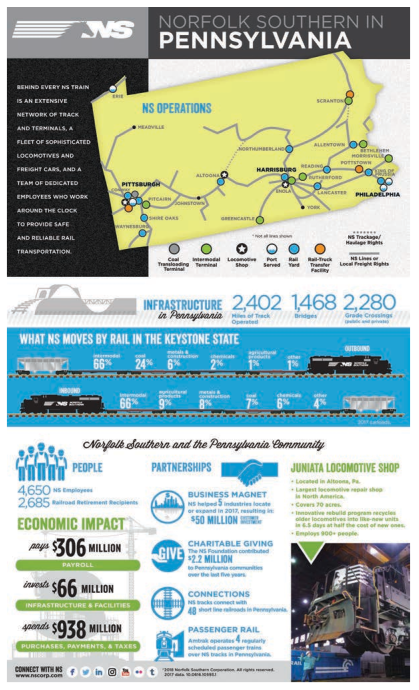
\includegraphics[width=0.33\linewidth,height=\textheight,keepaspectratio]{../img/NorfolkSouthern.png}

}

\caption{Norfolk Southern Corp., State Fact Sheets--Pennsylvania (2018)}

\end{figure}%

All told, when Mr.~Mallory sued, Norfolk Southern employed nearly 5,000
people in Pennsylvania. It maintained more than 2,400 miles of track
across the Commonwealth. Its 70-acre locomotive shop there was the
largest in North America. Contrary to what it says in its brief here,
the company even proclaimed itself a proud part of ``the Pennsylvania
Community.'' By 2020, too, Norfolk Southern managed more miles of track
in Pennsylvania than in any other State. And it employed more people in
Pennsylvania than it did in Virginia, where its headquarters was
located. Nor are we conjuring these statistics out of thin air. The
company itself highlighted its ``intrastate activities'' in the
proceedings below. 266 A.3d, at 560, 563 (discussing the firm's
``extensive operations in Pennsylvania,'' including ``2,278 miles of
track,'' ``eleven rail yards,'' and ``three locomotive repair shops'').
Given all this, on what plausible account could \emph{International
Shoe}'s concerns with ``fair play and substantial justice'' require a
Pennsylvania court to turn aside Mr.~Mallory's suit?

Perhaps sensing its arguments from fairness meet a dead end, Norfolk
Southern ultimately heads in another direction altogether. It suggests
the Due Process Clause separately prohibits one State from infringing on
the sovereignty of another State through exorbitant claims of personal
jurisdiction. And, in candor, the company is half right. Some of our
personal jurisdiction cases have discussed the federalism implications
of one State's assertion of jurisdiction over the corporate residents of
another. But that neglects an important part of the story. To date, our
personal jurisdiction cases have never found a Due Process Clause
problem sounding in federalism when an out-of-state defendant submits to
suit in the forum State. After all, personal jurisdiction is a personal
defense that may be waived or forfeited.

That leaves Norfolk Southern one final stand. It argues that it has not
really submitted to proceedings in Pennsylvania. The company does not
dispute that it has filed paperwork with Pennsylvania seeking the right
to do business there. It does not dispute that it has established an
office in the Commonwealth to receive service of process on any claim.
It does not dispute that it appreciated the jurisdictional consequences
attending these actions and proceeded anyway, presumably because it
thought the benefits outweighed the costs. But, in the name of the Due
Process Clause, Norfolk Southern insists we should dismiss all that as a
raft of meaningless formalities.

Taken seriously, this argument would have us undo not just
\emph{Pennsylvania Fire} but a legion of precedents that attach
jurisdictional consequences to what some might dismiss as mere
formalities. Consider some examples we have already encountered. In a
typical general jurisdiction case under \emph{International Shoe}, a
company is subject to suit on any claim in a forum State only because of
its decision to file a piece of paper there (a certificate of
incorporation). The firm is amenable to suit even if all of its
operations are located elsewhere and even if its certificate only sits
collecting dust on an office shelf for years thereafter. Then there is
the tag rule. The invisible state line might seem a trivial thing. But
when an individual takes one step off a plane after flying from New
Jersey to California, the jurisdictional consequences are immediate and
serious.

Consider, too, just a few other examples. A defendant who appears
``specially'' to contest jurisdiction preserves his defense, but one who
forgets can lose his. Failing to comply with certain pre-trial court
orders, signing a contract with a forum selection clause, accepting an
in-state benefit with jurisdictional strings attached---all these
actions as well can carry with them profound consequences for personal
jurisdiction.

The truth is, under our precedents a variety of ``actions of the
defendant'' that may seem like technicalities nonetheless can ``amount
to a legal submission to the jurisdiction of a court.'' That was so
before \emph{International Shoe}, and it remains so today. Should we
overrule them all? Taking Norfolk Southern's argument seriously would
require just that. But, tellingly, the company does not follow where its
argument leads or even acknowledge its implications. Instead, Norfolk
Southern asks us to pluck out and overrule just one longstanding
precedent that it happens to dislike. We decline the invitation. There
is no fair play or substantial justice in that.

Not every case poses a new question. This case poses a very old question
indeed---one this Court resolved more than a century ago in
\emph{Pennsylvania Fire}. Because that decision remains the law, the
judgment of the Supreme Court of Pennsylvania is vacated, and the case
is remanded.

\subsubsection{Justice Barrett, with whom The Chief Justice, Justice
Kagan, and Justice Kavanaugh join,
dissenting.}\label{justice-barrett-with-whom-the-chief-justice-justice-kagan-and-justice-kavanaugh-join-dissenting.}

For 75 years, we have held that the Due Process Clause does not allow
state courts to assert general jurisdiction over foreign defendants
merely because they do business in the State. \emph{International Shoe
Co.~v. Washington}. Pennsylvania nevertheless claims general
jurisdiction over all corporations that lawfully do business within its
borders. As the Commonwealth's own courts recognized, that flies in the
face of our precedent. See \emph{Daimler AG v. Bauman}.

The Court finds a way around this settled rule. All a State must do is
compel a corporation to register to conduct business there (as every
State does) and enact a law making registration sufficient for suit on
any cause (as every State could do). Then, every company doing business
in the State is subject to general jurisdiction based on implied
``consent''---not contacts. That includes suits, like this one, with no
connection whatsoever to the forum.

Such an approach does not formally overrule our traditional
contacts-based approach to jurisdiction, but it might as well. By
relabeling their long-arm statutes, States may now manufacture
``consent'' to personal jurisdiction. Because I would not permit state
governments to circumvent constitutional limits so easily, I
respectfully dissent.

\subsubsection{I}\label{i-5}

\paragraph{A}\label{a-2}

Personal jurisdiction is the authority of a court to issue a judgment
that binds a defendant. If a defendant submits to a court's authority,
the court automatically acquires personal jurisdiction. But if a
defendant contests the court's authority, the court must determine
whether it can nevertheless assert coercive power over the defendant.
That calculus turns first on the statute or rule defining the persons
within the court's reach. It depends next on the Due Process Clause,
which guards a defendant's right to resist the judicial authority of a
sovereign to which it has an insufficient tie. The Clause has the
companion role of ensuring that state courts ``do not reach out beyond
the limits imposed on them by their status as coequal sovereigns in a
federal system.''

Our precedent divides personal jurisdiction into two categories:
specific and general. Both are subject to the demands of the Due Process
Clause. Specific jurisdiction, as its name suggests, allows a state
court to adjudicate specific claims against a defendant. When a
defendant ``purposefully avails itself of the privilege of conducting
activities within the forum State,'' that State's courts may adjudicate
claims that `` `arise out of or relate to the defendant's contacts' with
the forum''.

General jurisdiction, by contrast, allows a state court to adjudicate
``\,`any and all claims' brought against a defendant.'' This sweeping
authority exists only when the defendant's connection to the State is
tight---so tight, in fact, that the defendant is ``\,`at home'\,''
there. An individual is typically ``at home'' in her domicile, and a
corporation is typically ``at home'' in both its place of incorporation
and principal place of business. Absent an exceptional circumstance,
general jurisdiction is cabined to these locations.

\paragraph{B}\label{b-2}

This case involves a Pennsylvania statute authorizing courts to exercise
general jurisdiction over corporations that are not ``at home'' in the
Commonwealth. All foreign corporations must register to do business in
Pennsylvania, and all registrants are subject to suit on ``any cause''
in the Commonwealth's courts. Section 5301 thus purports to empower
Pennsylvania courts to adjudicate any and all claims against
corporations doing business there.

As the Pennsylvania Supreme Court recognized, this statute ``clearly,
palpably, and plainly violates the Constitution.'' Look no further than
\emph{BNSF R. Co.~v. Tyrrell}, a case with remarkably similar
facts---and one that the Court conspicuously ignores. There, we assessed
whether Montana's courts could exercise general jurisdiction over the
BNSF railroad. No plaintiff resided in Montana or suffered an injury
there. Like Mallory, one of the plaintiffs alleged that the railroad
exposed him to toxic substances that caused his cancer. Like Norfolk
Southern, BNSF had tracks and employees in the forum, but it was neither
incorporated nor headquartered there. We rejected Montana's assertion of
general jurisdiction over BNSF because ``in-state business does not
suffice to permit the assertion of general jurisdiction over claims that
are unrelated to any activity occurring in {[}the State{]}.''
\emph{Daimler} and \emph{Goodyear}, we explained, could not have made
that any clearer.

The same rule applies here. The Pennsylvania statute announces that
registering to do business in the Commonwealth ``shall constitute a
sufficient basis'' for general jurisdiction. But as our precedent makes
crystal clear, simply doing business is insufficient. Absent an
exceptional circumstance, a corporation is subject to general
jurisdiction only in a State where it is incorporated or has its
principal place of business. Adding the antecedent step of registration
does not change that conclusion. If it did, ``every corporation would be
subject to general jurisdiction in every state in which it registered,
and Daimler's ruling would be robbed of meaning by a back-door thief.''

\subsubsection{II}\label{ii-5}

\paragraph{A}\label{a-3}

The Court short-circuits this precedent by characterizing this case as
one about consent rather than contacts-based jurisdiction. Consent is an
established basis for personal jurisdiction, which is, after all, a
waivable defense. ``A variety of legal arrangements have been taken to
represent express or implied consent to the personal jurisdiction of the
court,'' including contract, stipulation, and in-court appearance.
Today, the Court adds corporate registration to the list.

This argument begins on shaky ground, because Pennsylvania itself does
not treat registration as synonymous with consent. Section 5301(a)(2)(i)
baldly asserts that ``qualification as a foreign corporation'' in the
Commonwealth is a sufficient hook for general jurisdiction. The next
subsection (invoked by neither Mallory nor the Court) permits the
exercise of general jurisdiction over a corporation based on ``consent,
to the extent authorized by the consent.'' If registration were actual
consent, one would expect to see some mention of jurisdiction in Norfolk
Southern's registration paperwork---which is instead wholly silent on
the matter. What Mallory calls ``consent'' is what the Pennsylvania
Supreme Court called ``compelled submission to general jurisdiction by
legislative command.'' Corporate registration triggers a statutory
repercussion, but that is not ``consent'' in a conventional sense of the
word.

To pull §5301(a)(2)(i) under the umbrella of consent, the Court,
following Mallory, casts it as setting the terms of a bargain: In
exchange for access to the Pennsylvania market, a corporation must allow
the Commonwealth's courts to adjudicate any and all claims against it,
even those (like Mallory's) having nothing to do with Pennsylvania.
Everyone is charged with knowledge of the law, so corporations are on
notice of the deal. By registering, they agree to its terms.

While this is a clever theory, it falls apart on inspection. The Court
grounds consent in a corporation's choice to register with knowledge
(constructive or actual) of the jurisdictional consequences. But on that
logic, any long-arm statute could be said to elicit consent. Imagine a
law that simply provides, ``any corporation doing business in this State
is subject to general jurisdiction in our courts.'' Such a law defies
our precedent, which, again, holds that ``in-state business does not
suffice to permit the assertion of general jurisdiction.'' Yet this
hypothetical law, like the Pennsylvania statute, gives notice that
general jurisdiction is the price of doing business. And its ``notice''
is no less ``clear'' than Pennsylvania's. So on the Court's reasoning,
corporations that choose to do business in the State impliedly consent
to general jurisdiction. The result: A State could defeat the Due
Process Clause by adopting a law at odds with the Due Process Clause.

That makes no sense. If the hypothetical statute overreaches, then
Pennsylvania's does too. As the United States observes, ``invoking the
label `consent' rather than `general jurisdiction' does not render
Pennsylvania's long-arm statute constitutional.'' Brief for United
States as Amicus Curiae 4. Yet the Court takes this route without so
much as acknowledging its circularity.

\paragraph{B}\label{b-3}

While our due process precedent permits States to place reasonable
conditions on foreign corporations in exchange for access to their
markets, there is nothing reasonable about a State extracting consent in
cases where it has ``no connection whatsoever.'' The Due Process Clause
protects more than the rights of defendants---it also protects
interstate federalism. We have emphasized this principle in case after
case. For instance, in Hanson v. Denckla, we stressed that
``restrictions'' on personal jurisdiction ``are more than a guarantee of
immunity from inconvenient or distant litigation. They are a consequence
of territorial limitations on the power of the respective States.'' In
\emph{World-Wide Volkswagen}, we explained that ``even if the defendant
would suffer minimal or no inconvenience from being forced to litigate
before the tribunals of another State the Due Process Clause, acting as
an instrument of interstate federalism, may sometimes act to divest the
State of its power to render a valid judgment.'' And in
\emph{Bristol-Myers}, we reinforced that ``this federalism interest may
be decisive.'' A defendant's ability to waive its objection to personal
jurisdiction reflects that the Clause protects, first and foremost, an
individual right. But when a State announces a blanket rule that ignores
the territorial boundaries on its power, federalism interests are
implicated too.

Pennsylvania's effort to assert general jurisdiction over every company
doing business within its borders infringes on the sovereignty of its
sister States in a way no less ``exorbitant'' and ``grasping'' than
attempts we have previously rejected. Conditions on doing in-state
business cannot be ``inconsistent with those rules of public law which
secure the jurisdiction and authority of each State from encroachment by
all others.'' Permitting Pennsylvania to impose a blanket claim of
authority over controversies with no connection to the Commonwealth
intrudes on the prerogatives of other States---domestic and foreign---to
adjudicate the rights of their citizens and enforce their own laws.

The plurality's response is to fall back, yet again, on ``consent.'' In
its view, because a defendant can waive its personal jurisdiction right,
a State can never overreach in demanding its relinquishment. That is not
how we treat rights with structural components. The right to remove a
case to federal court, for instance, is primarily personal---it secures
for a nonresident defendant a federal forum thought to be more
impartial. At the same time, however, it serves federal interests by
ensuring that federal courts can vindicate federal rights. Recognizing
this dual role, we have rejected efforts of States to require defendants
to relinquish this (waivable) right to removal as a condition of doing
business. The same logic applies here. Pennsylvania's power grab
infringes on more than just the rights of defendants---it upsets the
proper role of the States in our federal system.

\subsubsection{III}\label{iii-4}

\paragraph{A}\label{a-4}

The plurality attempts to minimize the novelty of its conclusion by
pointing to our decision in \emph{Burnham v. Superior Court of Cal}.
There, we considered whether ``tag jurisdiction''---personal service
upon a defendant physically present in the forum State---remains an
effective basis for general jurisdiction after \emph{International
Shoe}. We unanimously agreed that it does. The plurality claims that
registration jurisdiction for a corporation is just as valid as the
``tag jurisdiction'' that we approved in \emph{Burnham}. But in drawing
this analogy, the plurality omits any discussion of \emph{Burnham}'s
reasoning.

In \emph{Burnham}, we acknowledged that tag jurisdiction would not
satisfy the contacts-based test for general jurisdiction. Nonetheless,
we reasoned that tag jurisdiction is ``both firmly approved by tradition
and still favored,'' making it ``one of the continuing traditions of our
legal system that defines the due process standard of 'traditional
notions of fair play and substantial justice. \emph{Burnham} thus
permits a longstanding and still-accepted basis for jurisdiction to pass
\emph{International Shoe}'s test.

General-jurisdiction-by-registration flunks both of these prongs: It is
neither ``firmly approved by tradition'' nor ``still favored.'' Thus,
the plurality's analogy to tag jurisdiction is superficial at best.

Start with the second prong. In \emph{Burnham}, ``we did not know of a
single state that had abandoned in-state service as a basis of
jurisdiction.'' Here, as Mallory concedes, Pennsylvania is the only
State with a statute treating registration as sufficient for general
jurisdiction. Indeed, quite a few have jettisoned the jurisdictional
consequences of corporate registration altogether---and in no uncertain
terms. With the Pennsylvania Legislature standing alone, the plurality
does not even attempt to describe this method of securing general
jurisdiction as ``still favored,'' or reflective of ``our common
understanding now''. Quite the opposite: The plurality denigrates ``the
spirit of our age''---reflected by the vast majority of States---and
appeals to its own notions of fairness.

The past is as fatal to the plurality's theory as the present.
\emph{Burnham's} tradition prong asks whether a method for securing
jurisdiction was ``shared by American courts at the crucial
time''---``1868, when the Fourteenth Amendment was adopted.'' But the
plurality cannot identify a single case from that period supporting its
theory. In fact, the evidence runs in the opposite direction. Statutes
that required the appointment of a registered agent for service of
process were far more modest than Pennsylvania's. And even when a
statute was written more broadly, state courts generally understood it
to implicitly limit jurisdiction to suits with a connection to the
forum. The state reporters are replete with examples of judicial
decisions that stood by the then-prevailing rule: Compliance with a
registration law did not subject a foreign corporation to suit on any
cause in a State, but only those related to the forum. Our cases from
this era articulate the same line. Although ``plaintiffs typically did
not sue defendants in fora that had no rational relation to causes of
action,'' courts repeatedly turned them away when they did.

\paragraph{B}\label{b-4}

Sidestepping \emph{Burnham}'s logic, the plurality seizes on its
bottom-line approval of tag jurisdiction. According to the plurality,
tag jurisdiction (based on physical presence) and registration
jurisdiction (based on deemed consent) are essentially the same
thing---so by blessing one, \emph{Burnham} blessed the other. The
plurality never explains why they are the same, even though---as we have
just discussed---more than a century's worth of law treats them as
distinct. The plurality's rationale seems to be that if a person is
subject to general jurisdiction anywhere she is present, then a
corporation should be subject to general jurisdiction anywhere it does
business. That is not only a non sequitur---it is ``contrary to the
historical rationale of \emph{International Shoe}.''

Before \emph{International Shoe}, a state court's power over a person
turned strictly on ``service of process within the State'' (presence)
``or her voluntary appearance'' (consent). \emph{Pennoyer v. Neff}. In
response to changes in interstate business and transportation in the
late 19th and early 20th centuries, States deployed new legal fictions
designed to secure the presence or consent of nonresident individuals
and foreign corporations. For example, state laws required nonresident
drivers to give their ``implied consent'' to be sued for their in-state
accidents as a condition of using the road. And foreign corporations, as
we have discussed, were required by statute to ``consent'' to the
appointment of a resident agent, so that the company could then be
constructively ``present'' for in-state service.

As Justice Scalia explained, such extensions of ``consent and presence
were purely fictional'' and can no longer stand after
\emph{International Shoe}. The very point of \emph{International Shoe}
was to ``cast aside'' the legal fictions built on the old territorial
approach to personal jurisdiction and replace them with its
contacts-based test. In Burnham, we upheld tag jurisdiction because it
is not one of those fictions---it is presence. By contrast,
Pennsylvania's registration statute is based on deemed consent. And this
kind of legally implied consent is one of the very fictions that our
decision in \emph{International Shoe} swept away.

\paragraph{C}\label{c}

Neither JUSTICE ALITO nor the plurality seriously contests this history.
Nor does either deny that Mallory's theory would gut \emph{Daimler}.
Instead, they insist that we already decided this question in a
pre-\emph{International Shoe} precedent: \emph{Pennsylvania Fire}.

The Court asserts that \emph{Pennsylvania Fire} controls our decision
today. I disagree. The case was ``decided before this Court's
transformative decision on personal jurisdiction in \emph{International
Shoe},'' and we have already stated that ``prior decisions that are
inconsistent with this standard are overruled''. \emph{Pennsylvania
Fire} fits that bill. Time and again, we have reinforced that ``\,`doing
business' tests''---like those ``framed before specific jurisdiction
evolved in the United States''---are not a valid basis for general
jurisdiction. The only innovation of Pennsylvania's statute is to make
``doing business'' synonymous with ``consent.'' If \emph{Pennsylvania
Fire} endorses that trick, then \emph{Pennsylvania Fire} is no longer
good law.

The plurality tries to get around \emph{International Shoe} by claiming
that it did no more than expand jurisdiction, affecting nothing that
came before it. That is as fictional as the old concept of ``corporate
presence'' on which the plurality relies. We have previously abandoned
even ``ancient'' bases of jurisdiction for incompatibility with
\emph{International Shoe}. And we have repeatedly reminded litigants not
to put much stock in our pre-\emph{International Shoe} decisions.
Daimler itself reinforces that pre-\emph{International Shoe} decisions
``should not attract heavy reliance today.'' Over and over, we have
reminded litigants that \emph{International Shoe} is ``canonical,''
``seminal,'' ``pathmarking,'' and even ``momentous''---to give just a
few examples. Yet the Court acts as if none of this ever happened.

In any event, I doubt \emph{Pennsylvania Fire} would control this case
even if it remained valid. \emph{Pennsylvania Fire} distinguished
between express consent (that is, consent ``actually conferred by the
document'') and deemed consent (inferred from doing business). As Judge
Learned Hand emphasized in a decision invoked by the plurality, without
``express consent,'' the normal rules apply.

The express power of attorney in \emph{Pennsylvania Fire} ``made service
on the insurance superintendent the equivalent of a corporate vote that
had accepted service in this specific case.'' Norfolk Southern, by
contrast, ``executed no document like the power of attorney there.'' The
Court makes much of what Norfolk Southern did write on its forms: It
named a ``Commercial Registered Office Provider,'' it notified
Pennsylvania of a merger, and it paid \$70 to update its paperwork. None
of those documents use the word ``agent,'' nothing hints at the word
``jurisdiction,'' and (as the Pennsylvania Supreme Court explained)
nothing about that registration is ``voluntary.'' Consent in
\emph{Pennsylvania Fire} was contained in the document itself; here it
is deemed by statute. If ``mere formalities'' matter as much as the
plurality says they do, it should respect this one too.

\subsubsection{IV}\label{iv-1}

By now, it should be clear that the plurality's primary approach to this
case is to look past our personal jurisdiction precedent. Relying on a
factsheet downloaded from the internet, for instance, the plurality
argues that Norfolk Southern is such a ``part of `the Pennsylvania
Community,'\,'' and does so much business there, that its ``presence''
in Pennsylvania is enough to require it to stand for suits having
nothing to do with the Commonwealth. In Daimler, however, we roundly
rejected the plaintiff's request that we ``approve the exercise of
general jurisdiction in every State in which a corporation `engages in a
substantial, continuous, and systematic course of business.'\,'' The
established test---which the plurality barely acknowledges---is whether
the corporation is ``at home'' in the State. ``A corporation that
operates in many places,'' and must therefore register in just as many,
``can scarcely be deemed at home in all of them.''

Critics of Daimler and Goodyear may be happy to see them go. And make no
mistake: They are halfway out the door. If States take up the Court's
invitation to manipulate registration, Daimler and Goodyear will be
obsolete, and, at least for corporations, specific jurisdiction will be
``superfluous.'' Because I would not work this sea change, I
respectfully dissent.

\subsection{Synthesis: Personal Jurisdiction
Analysis}\label{synthesis-personal-jurisdiction-analysis}

\begin{figure}[H]

{\centering 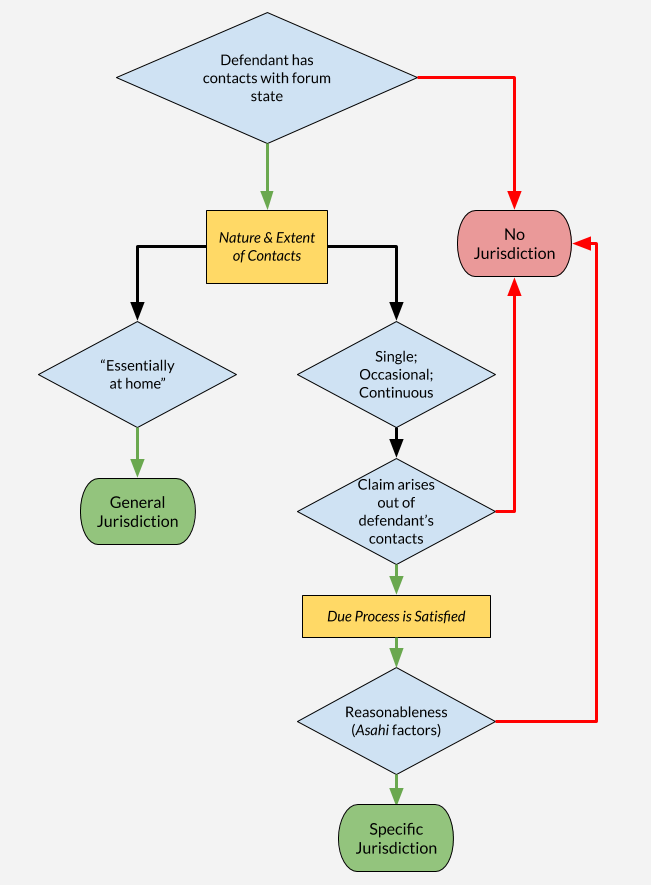
\includegraphics[width=0.85\linewidth,height=\textheight,keepaspectratio]{../img/personal-jurisdiction.png}

}

\caption{Personal Jurisdiction Flowchart}

\end{figure}%

\section{Statutory Authorization: Long-Arm
Statutes}\label{statutory-authorization-long-arm-statutes}

\begin{figure}[H]

{\centering 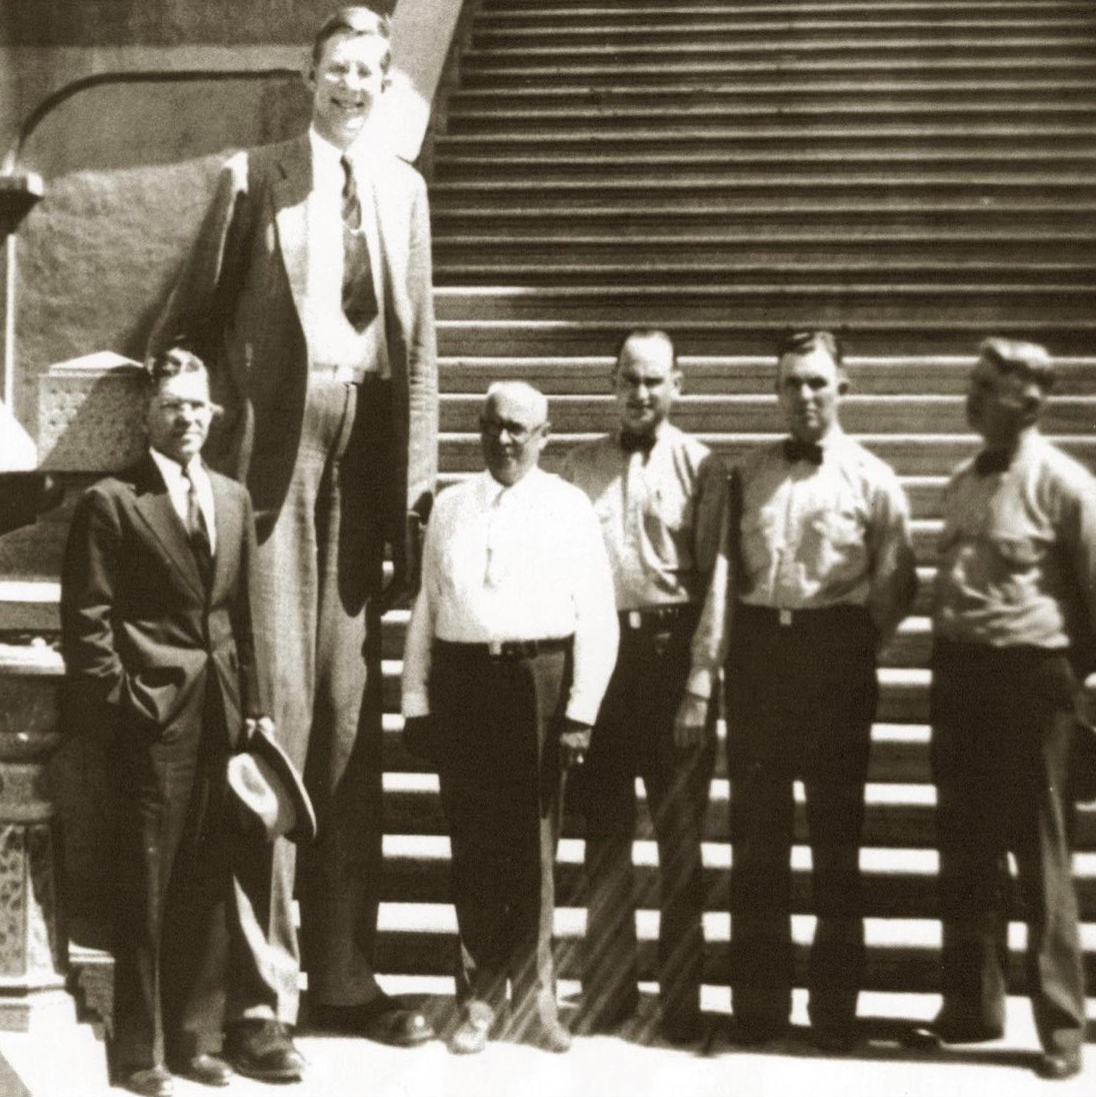
\includegraphics[width=0.66\linewidth,height=\textheight,keepaspectratio]{../img/Long-Arm.jpg}

}

\caption{Robert Wadlow, the tallest human in history, visiting Folsom
Prison in 1939 as a spokesman for the International Shoe Company.}

\end{figure}%

Within the outer bounds allowed under the constitutional due process
standard, the exercise of personal jurisdiction are subject to
additional limits under state ``long-arm'' statutes. There are two types
of long-arm statute.

\subsubsection{Enumerated Statutes}\label{enumerated-statutes}

Enumerated long-arm statutes identify particular circumstances in which
a state's courts may exercise jurisdiction over a non-resident. The New
York long-arm statute is an example:

\paragraph{NY CPLR §302: Personal jurisdiction by acts of
non-domiciliaries.}\label{ny-cplr-302-personal-jurisdiction-by-acts-of-non-domiciliaries.}

\emph{(a) Acts which are the basis of jurisdiction. As to a cause of
action arising from any of the acts enumerated in this section, a court
may exercise personal jurisdiction over any non-domiciliary, or his
executor or administrator, who in person or through an agent:}

\begin{itemize}
\item
  \emph{1. transacts any business within the state or contracts anywhere
  to supply goods or services in the state; or}
\item
  \emph{2. commits a tortious act within the state, except as to a cause
  of action for defamation of character arising from the act; or}
\item
  \emph{3. commits a tortious act without the state causing injury to
  person or property within the state, except as to a cause of action
  for defamation of character arising from the act, if he}

  \begin{itemize}
  \item
    \emph{(i) regularly does or solicits business, or engages in any
    other persistent course of conduct, or derives substantial revenue
    from goods used or consumed or services rendered, in the state, or}
  \item
    \emph{(ii) expects or should reasonably expect the act to have
    consequences in the state and derives substantial revenue from
    interstate or international commerce; or}
  \end{itemize}
\item
  \emph{4. owns, uses or possesses any real property situated within the
  state.}
\end{itemize}

\emph{(b) Personal jurisdiction over non-resident defendant in
matrimonial actions or family court proceedings. A court in any
matrimonial action or family court proceeding involving a demand for
support, alimony, maintenance, distributive awards or special relief in
matrimonial actions may exercise personal jurisdiction over the
respondent or defendant notwithstanding the fact that he or she no
longer is a resident or domiciliary of this state, or over his or her
executor or administrator, if the party seeking support is a resident of
or domiciled in this state at the time such demand is made, provided
that this state was the matrimonial domicile of the parties before their
separation, or the defendant abandoned the plaintiff in this state, or
the claim for support, alimony, maintenance, distributive awards or
special relief in matrimonial actions accrued under the laws of this
state or under an agreement executed in this state. The family court may
exercise personal jurisdiction over a non-resident respondent to the
extent provided in sections one hundred fifty-four and one thousand
thirty-six and article five-B of the family court act and article five-A
of the domestic relations law.}

\emph{(c) Effect of appearance. Where personal jurisdiction is based
solely upon this section, an appearance does not confer such
jurisdiction with respect to causes of action not arising from an act
enumerated in this section.}

\emph{(d) Foreign defamation judgment. The courts of this state shall
have personal jurisdiction over any person who obtains a judgment in a
defamation proceeding outside the United States against any person who
is a resident of New York or is a person or entity amenable to
jurisdiction in New York who has assets in New York or may have to take
actions in New York to comply with the judgment, for the purposes of
rendering declaratory relief with respect to that person's liability for
the judgment, and/or for the purpose of determining whether said
judgment should be deemed non-recognizable pursuant to section
fifty-three hundred four of this chapter, to the fullest extent
permitted by the United States constitution, provided:}

\begin{itemize}
\item
  \emph{1. the publication at issue was published in New York, and}
\item
  \emph{2. that resident or person amenable to jurisdiction in New York
  (i) has assets in New York which might be used to satisfy the foreign
  defamation judgment, or (ii) may have to take actions in New York to
  comply with the foreign defamation judgment. The provisions of this
  subdivision shall apply to persons who obtained judgments in
  defamation proceedings outside the United States prior to and/or after
  the effective date of this subdivision.}
\end{itemize}

Under an enumerated long-arm statute, determining whether the court may
exercise personal jurisdiction requires a two-step analysis:

\begin{enumerate}
\def\labelenumi{(\arabic{enumi})}
\item
  Does the case fall within one (or more) of the circumstances
  enumerated in the statute?
\item
  If so, does the defendant have the requisite contacts with the forum
  state to satisfy the constitutional due process standard?
\end{enumerate}

\subsubsection{Constitutional Limit
Statutes}\label{constitutional-limit-statutes}

This type of long-arm statute grants a state's courts jurisdiction to
the full extent permitted under the Constitution. The California
long-arm statute is an example:

\paragraph{Cal. Code Civ. Proc §410.10: Jurisdiction
exercisable.}\label{cal.-code-civ.-proc-410.10-jurisdiction-exercisable.}

\emph{A court of this state may exercise jurisdiction on any basis not
inconsistent with the Constitution of this state or of the United
States.}

Under this type of long-arm statute, the same analysis (i.e.~does the
defendant have minimum contacts with the forum state?) answers both the
statutory and constitutional question.

Some enumerated long-arm statutes have been interpreted as authorizing
the exercise of jurisdiction to the full extent permitted under the
constitution. See, e.g., \emph{Dillon v. Numismatic Funding Corp.}, 291
N.C. 674, 676 (1977) (``By the enactment of
\href{https://bit.ly/3Li9KAB}{G.S. 1-75.4(1)(d)}, it is apparent that
the General Assembly intended to make available to the North Carolina
courts the full jurisdictional powers permissible under federal due
process.'')

\section{Review Questions}\label{review-questions-1}

\subsubsection{Question 1}\label{question-1}

Mrs.~Potter, a wealthy resident of Philadelphia, decides that the time
has come to make provisions for her children after her death. She
creates a trust, administered by the Delaware Bank \& Trust Company
(located, naturally enough, in Delaware). Under the terms of the trust,
after Mrs.~Potter's death, her daughter Dora will receive whatever money
remains in the trust account. She also writes a will, leaving the
remainder of her estate to her other daughter, Polly.

A year later, Mrs.~Potter decides to move to Cocoanut Manor, a luxurious
retirement community in Florida. There she meets Mr.~Hammer, the genial
grifter who developed Cocoanut Manor in the hopes of attracting a steady
supply of wealthy victims for his cons. Mrs.~Potter, smitten by Hammer's
charm and believing he is the true love of her life, contacts the
Delaware bank and directs them to make Mr.~Hammer the trust beneficiary
in place of her daughter Dora, who hasn't even bothered to write or call
since Mrs.~Potter moved to Florida.

A few months later, Mrs.~Potter dies in a tragic shuffleboard accident.
Dora Potter is chagrined to discover that the trust funds, now totalling
\$1.4 million, will go to Mr.~Hammer instead of her. She brings a
lawsuit in a Florida court, challenging the validity of the trust. Polly
Potter, who despises her sister, also joins the suit as a co-plaintiff,
arguing that the money in the trust should also go to her as part of
Mrs.~Potter's estate under the will. Because the Bank is in control of
the trust account, it is named as a co-defendant in the suit.

\emph{Does the Florida court have personal jurisdiction over the Bank?}

\subsubsection{Question 2}\label{question-2}

Dan \& Pat, both residents of Pennsylvania, are partners in a Delaware
business. The business fails and a disagreement arises between Dan \&
Pat over the division of the partnership's remaining assets. Deciding to
get away from it all, Dan moves to Idaho. Pat now wants to sue Dan over
the partnership dispute. Each state's long-arm statute provides for
jurisdiction to the full extent permitted under the U.S. Constitution.

\emph{In which state(s) may Pat sue?}

\subsubsection{Question 3}\label{question-3}

\emph{Same facts as previous question, but assume Pat has not sued Dan.}

Pat has a vacation home on the Jersey shore. While Pat is spending the
weekend there, Dan arranges to serve Pat with a complaint and summons in
a suit Dan has filed in New Jersey court, claiming that Pat owes Dan
\$25,000 arising from their business partnership. May the New Jersey
court assert jurisdiction?

\begin{enumerate}
\def\labelenumi{\alph{enumi}.}
\item
  Yes, because Pat owns property in New Jersey
\item
  Yes, because Pat was personally served with the complaint and summons
  while physically present in New Jersey.
\item
  No, because the suit does not arise from, and is unrelated to, Pat's
  contacts with New Jersey
\item
  No, because New Jersey is not Pat's permanent home
\end{enumerate}

\subsubsection{Question 4}\label{question-4}

Ronnie operates a gas station near U.S. Interstate 40 in Greensboro,
North Carolina. The station is frequented by locals and by interstate
travelers using I-40. Last summer, Ronnie changed a tire on an
automobile bearing Missitucky license plates. The car belonged to
Vivian, who was driving through Greensboro on the way home from vacation
in the Outer Banks. A few days later, after Vivian reached Missitucky,
the tire suddenly fell off, causing the car to swerve out of control and
hit an embankment. Vivian sued Ronnie in Missitucky state court,
alleging that the accident resulted in Ronnie's negligence in changing
the tire.

\emph{Assuming the Missitucky long-arm statute allows it, would the
exercise of personal jurisdiction over Ronnie be permissible under the
U.S. Constitution?}

\subsubsection{Question 5}\label{question-5}

Gerald Mayo sued Satan and his Staff, alleging that, on numerous
occasions, they caused him misery, made unwarranted threats against him,
and placed deliberate obstacles in his path, causing his downfall. Mayo
filed his suit in the U.S. District Court for the Western District of
Pennsylvania. Mayo resides in Pittsburgh, where the court is located.
Mayo lives in Slippery Rock, Pennsylvania. None of the defendants reside
in Pennsylvania.

\emph{On what basis might the court have personal jurisdiction over the
defendants?} See \href{../exhibits/Mayo_Satan.pdf}{\emph{U.S. ex rel.
Mayo v. Satan and His Staff}}, 54 F.R.D. 282 (W.D. Pa. 1971).

\chapter{Subject Matter Jurisdiction}\label{subject-matter-jurisdiction}

\section{Federal Question
Jurisdiction}\label{federal-question-jurisdiction}

\subsection{U.S. Constitution, Article
III}\label{u.s.-constitution-article-iii-1}

\subsubsection{Section 2}\label{section-2-1}

The judicial power shall extend to all cases, in law and equity, arising
under this Constitution, the laws of the United States, and treaties
made, or which shall be made, under their authority;

\subsection{28 U.S.C. § 1331}\label{u.s.c.-1331}

The district courts shall have original jurisdiction of all civil
actions arising under the Constitution, laws, or treaties of the United
States.

\subsection{Louisville \& Nashville R. Co.~v. Mottley (U.S.
1908)}\label{louisville-nashville-r.-co.-v.-mottley-u.s.-1908}

\subsubsection{Statement by Justice
Moody}\label{statement-by-justice-moody}

The {\marginnote{\begin{footnotesize}The remedy that the Mottleys sought
was ``specific performance'', i.e.~an order requiring the Railroad to
honor the free passes. This is a form a equitable relief, sometimes
available instead of money damages, which is the usual legal relief for
breach of contract. Prior to the advent of the Federal Rules of Civil
Procedure, different procedures applied to suits for equitable relief
and suits for legal relief. A suit in equity was commenced by filing a
``bill'', functionally equivalent to a complaint. You can
\href{../exhibits/Mottley-complaint.pdf}{read the Mottleys' bill
here}.\end{footnotesize}}} appellees (husband and wife), being residents
and citizens of Kentucky, brought this suit in equity in the circuit
court of the United States for the western district of Kentucky against
the appellant, a railroad company and a citizen of the same state. The
object of the suit was to compel the specific performance of the
following contract:

\begin{quote}
Louisville, Ky., Oct.~2d, 1871.

The Louisville \& Nashville Railroad Company, in consideration that E.
L. Mottley and wife, Annie E. Mottley, have this day released company
from all damages or claims for damages for injuries received by them on
the 7th of September, 1871, in consequence of a collision of trains on
the railroad of said company at Randolph's Station, Jefferson County,
Kentucky, hereby agrees to issue free passes on said railroad and
branches now existing or to exist, to said E. L. \& Annie E. Mottley for
the remainder of the present year, and thereafter to renew said passes
annually during the lives of said Mottley and wife or either of them.
\end{quote}

The bill alleged that in September, 1871, plaintiffs, while passengers
upon the defendant railroad, were injured by the defendant's negligence,
and released their respective claims for damages in consideration of the
agreement for transportation during their lives, expressed in the
contract. It is alleged that the contract was performed by the defendant
up to January 1, 1907, when the defendant declined to renew the passes.
{\marginnote{\begin{footnotesize}The
\href{https://www.archives.gov/legislative/features/hepburn}{Hepburn
Act} gave the Interstate Commerce Commission regulatory authority over
railroad shipping and passenger rates. The Act also restriced the
practice of giving rate rebates and free passes.\end{footnotesize}}} The
bill then alleges that the refusal to comply with the contract was based
solely upon that part of the act of Congress of June 29, 1906, which
forbids the giving of free passes or free transportation. The bill
further alleges: First, that the act of Congress referred to does not
prohibit the giving of passes under the circumstances of this case; and,
second, that, if the law is to be construed as prohibiting such passes,
it is in conflict with the 5th Amendment of the Constitution, because it
deprives the plaintiffs of their property without due process of law.
The defendant demurred to the bill. The judge of the circuit court
overruled the demurrer, entered a decree for the relief prayed for, and
the defendant appealed directly to this court.

\subsubsection{Opinion}\label{opinion}

Two questions of law were brought here by appeal. They are, first,
whether that part of the act of Congress of June 29, 1906, which forbids
the giving of free passes or the collection of any different
compensation for transportation of passengers than that specified in the
tariff filed, makes it unlawful to perform a contract for transportation
of persons, who in good faith, before the passage of the act, had
accepted such contract in satisfaction of a valid cause of action
against the railroad; and, second, whether the statute, if it should be
construed to render such a contract unlawful, is in violation of the
Fifth Amendment of the Constitution of the United States. We do not deem
it necessary, however, to consider either of these questions, because,
in our opinion, the court below was without jurisdiction of the cause.
Neither party has questioned that jurisdiction, but it is the duty of
this court to see to it that the jurisdiction of the Circuit Court,
which is defined and limited by statute, is not exceeded. This duty we
have frequently performed of our own motion.

There was no diversity of citizenship and it is not and cannot be
suggested that there was any ground of jurisdiction, except that the
case was a ``suit arising under the Constitution and laws of the United
States.'' It is the settled interpretation of these words, as used in
this statute, conferring jurisdiction, that a suit arises under the
Constitution and laws of the United States only when the plaintiff's
statement of his own cause of action shows that it is based upon those
laws or that Constitution. It is not enough that the plaintiff alleges
some anticipated defense to his cause of action and asserts that the
defense is invalidated by some provision of the Constitution of the
United States. Although such allegations show that very likely, in the
course of the litigation, a question under the Constitution would arise,
they do not show that the suit, that is, the plaintiff's original cause
of action, arises under the Constitution. In \emph{Tennessee} v.
\emph{Union \& Planters' Bank,} 152 U.S. 454, the plaintiff, the State
of Tennessee, brought suit in the Circuit Court of the United States to
recover from the defendant certain taxes alleged to be due under the
laws of the State. The plaintiff alleged that the defendant claimed an
immunity from the taxation by virtue of its charter, and that therefore
the tax was void, because in violation of the provision of the
Constitution of the United States, which forbids any State from passing
a law impairing the obligation of contracts. The cause was held to be
beyond the jurisdiction of the Circuit Court, the court saying, by
Mr.~Justice Gray, ``a suggestion of one party, that the other will or
may set up a claim under the Constitution or laws of the United States,
does not make the suit one arising under that Constitution or those
laws.''

The application of this rule to the case at bar is decisive against the
jurisdiction of the Circuit Court.

\subsection{\texorpdfstring{Note: Postscript to
\emph{Mottley}}{Note: Postscript to Mottley}}\label{note-postscript-to-mottley}

On remand, the Kentucky court held that the 1906 statute did not apply
to the Mottleys' free passes and ordered the railroad to continue
honoring the settlement agreement. \emph{Louisville \& Nashville R.
Co.~v. Mottley}, 133 Ky. 652 (1909). The case made its way back to the
U.S. Supreme Court, which once again ruled against the Mottleys. Holding
that the 1906 statute rendered the agreement to provide free passes
illegal, the Court reversed the order granting specific performance.
\href{https://scholar.google.com/scholar_case?case=15541627978206243212}{\emph{Louisville
\& Nashville R. Co.~v. Mottley}}, 219 US 467 (1911). That opinion did
not entirely foreclose the possibility of some other remedy for the
Mottleys:

\begin{quote}
Whether, without enforcing the contract in suit, the defendants in error
may, by some form of proceeding against the railroad company, recover or
restore the rights they had when the railroad collision occurred is a
question not before us, and we express no opinion on it.
\end{quote}

However, there is no record of anything further transpiring in the case.

Apart from the case for which he is remembered today, Erasmus Mottley
was apparently ``a prominent and influential business man'' and
unsuccessful candidate for public office. E. Polk Johnson (1912):
819-20.

\subsection{Grable \& Sons Metal Products, Inc.~v. Darue Engineering \&
Mfg. (U.S.
2005)}\label{grable-sons-metal-products-inc.-v.-darue-engineering-mfg.-u.s.-2005}

\subsubsection{Justice Souter delivered the opinion of the
Court.}\label{justice-souter-delivered-the-opinion-of-the-court.}

The question is whether want of a federal cause of action to try claims
of title to land obtained at a federal tax sale precludes removal to
federal court of a state action with nondiverse parties raising a
disputed issue of federal title law. We answer no, and hold that the
national interest in providing a federal forum for federal tax
litigation is sufficiently substantial to support the exercise of
federal-question jurisdiction over the disputed issue on removal, which
would not distort any division of labor between the state and federal
courts, provided or assumed by Congress.

\subsubsection{I}\label{i-6}

In 1994, {\marginnote{\begin{footnotesize}A \emph{quitclaim deed} is ``a
document by which a grantor conveys his or her present interest, if any,
in a given parcel of real property to a grantee without representing,
covenanting, or warranting that the title is good.''
\href{https://www.law.cornell.edu/wex/quitclaim_deed}{Wex Legal
Dictionary}.\end{footnotesize}}} the Internal Revenue Service seized
Michigan real property belonging to petitioner Grable \& Sons Metal
Products, Inc., to satisfy Grable's federal tax delinquency. Title 26
U.S.C. §6335 required the IRS to give notice of the seizure, and there
is no dispute that Grable received actual notice by certified mail
before the IRS sold the property to respondent Darue Engineering \&
Manufacturing. Although Grable also received notice of the sale itself,
it did not exercise its statutory right to redeem the property within
180 days of the sale, and after that period had passed, the Government
gave Darue a quitclaim deed.

Five years later, Grable brought a quiet title action in state court,
{\marginnote{\begin{footnotesize}``A quiet title action is a special
legal proceeding to determine ownership of real property. A party with a
claim of ownership to land can file an action to quiet title, which
serves as a sort of lawsuit against anyone and everyone else who has a
claim to the land. If the owner prevails in the quiet title action, no
further challenges to the title can be brought.''
\href{https://www.law.cornell.edu/wex/quiet_title_action}{Wex Legal
Dictionary}.\end{footnotesize}}} claiming that Darue's record title was
invalid because the IRS had failed to notify Grable of its seizure of
the property in the exact manner required by §6335(a), which provides
that written notice must be ``given by the Secretary to the owner of the
property or left at his usual place of abode or business.'' Grable said
that the statute required personal service, not service by certified
mail.

Darue removed the case to Federal District Court as presenting a federal
question, because the claim of title depended on the interpretation of
the notice statute in the federal tax law. The District Court declined
to remand the case at Grable's behest after finding that the ``claim
does pose a significant question of federal law,'' and ruling that
Grable's lack of a federal right of action to enforce its claim against
Darue did not bar the exercise of federal jurisdiction. On the merits,
the court granted summary judgment to Darue, holding that although §6335
by its terms required personal service, substantial compliance with the
statute was enough.

The Court of Appeals for the Sixth Circuit affirmed. On the
jurisdictional question, the panel thought it sufficed that the title
claim raised an issue of federal law that had to be resolved, and
implicated a substantial federal interest (in construing federal tax
law). The court went on to affirm the District Court's judgment on the
merits. We granted certiorari on the jurisdictional question alone, to
resolve a split within the Courts of Appeals on whether \emph{Merrell
Dow Pharmaceuticals Inc.~v. Thompson}, 478 U. S. 804 (1986), always
requires a federal cause of action as a condition for exercising
federal-question jurisdiction. We now affirm.

\subsubsection{II}\label{ii-6}

Darue was entitled to remove the quiet title action if Grable could have
brought it in federal district court originally, 28 U.S.C. §1441(a), as
a civil action ``arising under the Constitution, laws, or treaties of
the United States,'' §1331. This provision for federal-question
jurisdiction is invoked by and large by plaintiffs pleading a cause of
action created by federal law. There is, however, another longstanding,
if less frequently encountered, variety of federal ``arising under''
jurisdiction, this Court having recognized for nearly 100 years that in
certain cases federal-question jurisdiction will lie over state-law
claims that implicate significant federal issues. The doctrine captures
the commonsense notion that a federal court ought to be able to hear
claims recognized under state law that nonetheless turn on substantial
questions of federal law, and thus justify resort to the experience,
solicitude, and hope of uniformity that a federal forum offers on
federal issues.

The {\marginnote{\begin{footnotesize}Recall that, in \emph{Louisville \&
Nashville R. Co.~v. Mottley}, the Court held there was no federal
question jurisdiction even though the principal issue in that case was
the legality of the Mottleys' free passes under the 1906 federal
statute. How is \emph{Mottley} distinguishable from \emph{Smith v.
Kansas City Title \& Trust}?\end{footnotesize}}} classic example is
\emph{Smith v. Kansas City Title \& Trust Co.}, 255 U.S. 180 (1921), a
suit by a shareholder claiming that the defendant corporation could not
lawfully buy certain bonds of the National Government because their
issuance was unconstitutional. Although Missouri law provided the cause
of action, the Court recognized federal-question jurisdiction because
the principal issue in the case was the federal constitutionality of the
bond issue. \emph{Smith} thus held, in a somewhat generous statement of
the scope of the doctrine, that a state-law claim could give rise to
federal-question jurisdiction so long as it ``appears from the complaint
that the right to relief depends upon the construction or application of
{[}federal law{]}.''

The \emph{Smith} statement has been subject to some trimming to fit
earlier and later cases recognizing the vitality of the basic doctrine,
but shying away from the expansive view that mere need to apply federal
law in a state-law claim will suffice to open the ``arising under''
door. It has in fact become a constant refrain in such cases that
federal jurisdiction demands not only a contested federal issue, but a
substantial one, indicating a serious federal interest in claiming the
advantages thought to be inherent in a federal forum.

But even when the state action discloses a contested and substantial
federal question, the exercise of federal jurisdiction is subject to a
possible veto. For the federal issue will ultimately qualify for a
federal forum only if federal jurisdiction is consistent with
congressional judgment about the sound division of labor between state
and federal courts governing the application of §1331. Because
arising-under jurisdiction to hear a state-law claim always raises the
possibility of upsetting the state-federal line drawn (or at least
assumed) by Congress, the presence of a disputed federal issue and the
ostensible importance of a federal forum are never necessarily
dispositive; there must always be an assessment of any disruptive
portent in exercising federal jurisdiction.

These considerations have kept us from stating a ``single, precise,
all-embracing'' test for jurisdiction over federal issues embedded in
state-law claims between nondiverse parties. We have not kept them out
simply because they appeared in state raiment, but neither have we
treated ``federal issue'' as a password opening federal courts to any
state action embracing a point of federal law. Instead, the question is,
does a state-law claim necessarily raise a stated federal issue,
actually disputed and substantial, which a federal forum may entertain
without disturbing any congressionally approved balance of federal and
state judicial responsibilities.

\subsubsection{III}\label{iii-5}

This case warrants federal jurisdiction. Grable's state complaint must
specify ``the facts establishing the superiority of its claim,'' and
Grable has premised its superior title claim on a failure by the IRS to
give it adequate notice, as defined by federal law. Whether Grable was
given notice within the meaning of the federal statute is thus an
essential element of its quiet title claim, and the meaning of the
federal statute is actually in dispute; it appears to be the only legal
or factual issue contested in the case. The meaning of the federal tax
provision is an important issue of federal law that sensibly belongs in
a federal court. The Government has a strong interest in the ``prompt
and certain collection of delinquent taxes,'' and the ability of the IRS
to satisfy its claims from the property of delinquents requires clear
terms of notice to allow buyers like Darue to satisfy themselves that
the Service has touched the bases necessary for good title. The
Government thus has a direct interest in the availability of a federal
forum to vindicate its own administrative action, and buyers (as well as
tax delinquents) may find it valuable to come before judges used to
federal tax matters. Finally, because it will be the rare state title
case that raises a contested matter of federal law, federal jurisdiction
to resolve genuine disagreement over federal tax title provisions will
portend only a microscopic effect on the federal-state division of
labor.

\emph{Merrell Dow Pharmaceuticals Inc.~v. Thompson}, 478 U. S. 804
(1986), on which Grable rests its position, is not to the contrary.
\emph{Merrell Dow} considered a state tort claim resting in part on the
allegation that the defendant drug company had violated a federal
misbranding prohibition, and was thus presumptively negligent under Ohio
law. The Court assumed that federal law would have to be applied to
resolve the claim, but after closely examining the strength of the
federal interest at stake and the implications of opening the federal
forum, held federal jurisdiction unavailable. Congress had not provided
a private federal cause of action for violation of the federal branding
requirement, and the Court found ``it would flout, or at least
undermine, congressional intent to conclude that federal courts might
nevertheless exercise federal-question jurisdiction and provide remedies
for violations of that federal statute solely because the violation is
said to be a `proximate cause' under state law.''

Because federal law provides for no quiet title action that could be
brought against Darue, Grable argues that there can be no federal
jurisdiction here, stressing some broad language in \emph{Merrell Dow}
that on its face supports Grable's position. But an opinion is to be
read as a whole, and \emph{Merrell Dow} cannot be read whole as
overturning decades of precedent, as it would have done by effectively
adopting the Holmes dissent in \emph{Smith}, and converting a federal
cause of action from a sufficient condition for federal-question
jurisdiction into a necessary one.

Accordingly, \emph{Merrell Dow} should be read in its entirety as
treating the absence of a federal private right of action as evidence
relevant to, but not dispositive of, the ``sensitive judgments about
congressional intent'' that §1331 requires. The absence of any federal
cause of action affected \emph{Merrell Dow's} result two ways. The Court
saw the fact as worth some consideration in the assessment of
substantiality. But its primary importance emerged when the Court
treated the combination of no federal cause of action and no preemption
of state remedies for misbranding as an important clue to Congress's
conception of the scope of jurisdiction to be exercised under §1331. The
Court saw the missing cause of action not as a missing federal door key,
always required, but as a missing welcome mat, required in the
circumstances, when exercising federal jurisdiction over a state
misbranding action would have attracted a horde of original filings and
removal cases raising other state claims with embedded federal issues.
For if the federal labeling standard without a federal cause of action
could get a state claim into federal court, so could any other federal
standard without a federal cause of action. And that would have meant a
tremendous number of cases.

As already indicated, however, a comparable analysis yields a different
jurisdictional conclusion in this case. Although Congress also indicated
ambivalence in this case by providing no private right of action to
Grable, it is the rare state quiet title action that involves contested
issues of federal law. Consequently, jurisdiction over actions like
Grable's would not materially affect, or threaten to affect, the normal
currents of litigation. Given the absence of threatening structural
consequences and the clear interest the Government, its buyers, and its
delinquents have in the availability of a federal forum, there is no
good reason to shirk from federal jurisdiction over the dispositive and
contested federal issue at the heart of the state-law title claim.

\subsection{Note: Understanding Grable}\label{note-understanding-grable}

In \emph{Grable}, the Supreme Court sought to clarify when a state-law
claim with an ``essential federal element'' falls within the
jurisdiction granted under §1331. This is not really an exception to the
``well-pleaded complaint'' rule in \emph{Mottley}. Under the
\emph{Grable} standard, the federal question must still arises on the
face of the complaint, i.e.~as one of the elements of the plaintiff's
claim, not a defense.

But the \emph{Grable} standard is an exception to the Holmes ``creation
test''. Even though state law creates the plaintiff's cause of action
(which, for Holmes, would mean the claim did not ``arise under'' federal
law), the presence of a federal issue as an element of the claim may
nonetheless confer federal jurisdiction under §1331.

\subsubsection{Rule}\label{rule}

A state-law claim raises a federal question, sufficient to confer
jurisdiction under §1331, where,

\begin{enumerate}
\def\labelenumi{\arabic{enumi}.}
\tightlist
\item
  An issue of federal law forms an \emph{essential part of plaintiff's
  claim} (not a defense),
\item
  The federal issue is \emph{actually disputed,} and
\item
  There is a \emph{substantial federal interest} at stake.
\end{enumerate}

\paragraph{Essential Federal Issue}\label{essential-federal-issue}

The federal issue is ``essential'' where the plaintiff's ``right to
relief depends upon the construction or application of the Constitution
or laws of the United States.'' \emph{Smith v. Kansas City Title \&
Trust Co.} (US 1921). This requirement will generally be satisfied where
the plaintiff relies on federal law to establish a right, interest, or
duty at issue in the case.

\paragraph{Federal Issue Is Actually
Disputed}\label{federal-issue-is-actually-disputed}

If there is no dispute between the parties over the federal issue as it
arises in the case, there is no need for the court to resolve the issue
and thus no reason to confer federal subject matter jurisdiction based
on that issue.

\paragraph{Substantial Federal
Interest}\label{substantial-federal-interest}

In assessing whether there is a ``substantial federal interest'', the
Supreme Court has considered these factors:

\begin{enumerate}
\def\labelenumi{\arabic{enumi}.}
\tightlist
\item
  Whether uniform interpretation and application of federal law is
  important for fulfilling federal policy
\item
  Whether allowing a federal forum for private litigants would undermine
  a federal statutory enforcement scheme
\item
  Whether providing a federal forum would upset the balance between the
  state and federal judicial systems
\end{enumerate}

\subsubsection{Illustrations}\label{illustrations}

\paragraph{Federal Issue}\label{federal-issue}

\textbf{Essential: Grable}: Grable brought a state-law ``quiet title''
claim against Darue, which purchased property that the IRS had seized
from Grable in satisfaction of a tax delinquency.

\begin{itemize}
\tightlist
\item
  • Under state law, Grable was required to specify ``the facts
  establishing the superiority of its claim'' to the property.
\end{itemize}

Under the federal statute governing the sale of property to satisfy tax
delinquencies, the IRS was supposed to give Grable written notice of the
seizure. The IRS sent Grable notice of the seizure by certified mail,
but Grable contended that the statute required personal service of the
notice. - • Grable argued that failure to satisfy the federal statutory
notice requirement rendered the sale of the property to Darue invalid. -
• Darue argued that, since Grable received actual notice of the seizure
and sale, but failed to exercise its
\href{https://www.law.cornell.edu/uscode/text/26/6337}{statutory right
to redeem the property} within 180 days of the sale, Darue's purchase of
the property was valid.

Grable's right to relief thus depended on the construction and
applicability of federal law (i.e.~whether service of the IRS notice by
certified mail satisfied the federal statute the lack of notice in the
form specified by federal law rendered the sale of the property void).
And this issue was actually in dispute between the parties.

The real focus of the suit was Grable's right under federal law not to
have its property seized by the IRS without proper notice. Grable was
merely using a state-law quiet title action as the means to vindicate
that right (because federal law itself didn't provide a remedy).

\textbf{Not Essential: Merrell Dow}: The plaintiffs brought state law
negligence and other tort claims against Merrell Dow for birth defects
allegedly resulting from a drug manufactured and marketed by Merrell
Dow.

\begin{itemize}
\tightlist
\item
  • The plaintiffs alleged that Merrell Dow's failure to warn about
  potential birth defects was negligent.
\end{itemize}

Under state tort law, one way a plaintiff could satisfy the negligence
element was by showing that the defendant failed to comply with an
applicable state or federal legal standard. - • The plaintiffs relied on
federal law for this purpose, asserting that FDA regulations required a
warning about potential birth defects.

The plaintiffs were not asserting rights under federal law. They were
simply using the FDA regulations as \emph{evidence} of what a reasonable
drug manufacturer would do, to establish negligence under state law.

\textbf{Not Essential: Gunn v. Minton}: Minton sued Gunn under state law
for attorney malpractice. The malpractice claim was based on a previous
suit in which Gunn had represented Minton as the plaintiff in a patent
infringement suit (governed by federal law).

Under state law, Minton was required to allege (and prove) that Gunn's
representation in the underlying suit was negligent, and that Gunn would
have prevailed in that suit but for Gunn's negligence.

\begin{itemize}
\item
  • Minton alleged that Gunn failed to raise a certain argument in the
  patent infringement suit, that a competent lawyer would have raised
  the argument, and that Minton would have won if Gunn had raised the
  argument.
\item
  • To decide whether the argument would have been successful, the court
  would have to apply federal patent law.
\end{itemize}

As in Merrell Dow, the suit wasn't really about Minton's rights under
federal law.

\begin{itemize}
\tightlist
\item
  • The patent law issue arose only as a benchmark for establishing
  whether Gunn suffered an injury as a result of negligent legal
  representation.
\end{itemize}

\paragraph{Federal Interest}\label{federal-interest}

\textbf{Substantial: Grable}: There is a strong federal interest in
uniform interpretation of the statutory requirements for seizures of
taxpayer property by the IRS. Inconsistent interpretations by various
state courts would subject the IRS to conflicting standards in carrying
out its tax enforcement responsibilities, and promote uncertainty about
the rights and interests of taxpayers and purchasers of seized property.

The absence of a private right of action to enforce the statutory notice
requirements in IRS tax seizures does not weigh against the exercise of
federal jurisdiction over state-law quiet title claims based on alleged
violations of the federal statutory requirements.

\begin{itemize}
\item
  • The federal statute provides no special enforcement mechanism for
  those requirements, so private suits aren't interfering with anything.
\item
  • But the federal statute gives individual taxpayers private rights,
  so it makes sense for federal courts to adjudicate claims that depend
  on whether those rights were violated.
\end{itemize}

Only rarely will a state-law quiet title claim depend on an issue of
federal law, so there is little risk of opening the floodgates to claims
that properly belong in state court. The strong federal interest at
stake justifies opening the federal courts to the relatively limited set
of cases in which the issue arises.

\textbf{Not Substantial: Merrell Dow}: While there is a federal interest
in uniform interpretation of drug labeling requirements under the
Federal Food, Drug, and Cosmetic Act (FDCA), that interest would not be
impaired by conflicting state court interpretations in the context of
state-law product liability claims.

\begin{itemize}
\tightlist
\item
  • Decisions in those cases would not affect any rights, interests, or
  duties under the FDCA itself.
\end{itemize}

The FDCA has its own mechanism for promoting uniform interpretation and
application, through exclusive enforcement by the FDA.

\begin{itemize}
\tightlist
\item
  • A state court determination in the negligence suit would not be
  binding in an enforcement action by the FDA.
\end{itemize}

The FDCA provides for exclusive enforcement by the FDA, and there is no
private right of action under the statute.

\begin{itemize}
\item
  • The statutory enforcement scheme evidences a Congressional intent
  that the federal courts not adjudicate private suits arising under the
  FDCA.
\item
  • Allowing plaintiffs to litigate FDCA non-compliance under the guise
  of state-law tort claims would undermine this statutory scheme.
\end{itemize}

The plaintiffs in these cases asserted routine state-law claims, in
which the federal issues were merely incidental to establishing the
defendants' liability under state law.

\begin{itemize}
\item
  • State law commonly allows plaintiffs to use federal legal standards
  as a baseline for establish the standard of care under state tort law.
\item
  • If every such case were regarded as arising under federal law for
  purposes of jurisdiction under §1331, this would effectively
  ``federalize'' much routine tort law, subjecting the federal courts to
  a flood of cases that raise no substantial federal interest, and
  interfering with the role of state courts as the primary forum for
  raising state-law claims.
\end{itemize}

\textbf{Not Substantial: Gunn v. Minton}: While there is a federal
interest in uniform interpretation of federal patent law, that interest
would not be impaired by conflicting state court interpretations in the
context of state-law attorney malpractice claims.

\begin{itemize}
\item
  • State court interpretations of federal patent law in the context of
  attorney malpractice claims do not actually affect any rights or
  interests under federal patent law.
\item
  • The federal issues arise only as counterfactual hypotheticals: what
  would have happened if the attorney had done something different?
\end{itemize}

Uniform interpretation and application of federal patent law, in cases
where rights under that law are actually at stake, is ensured by
exclusive federal jurisdiction over patent claims (i.e.~state courts may
not hear those claims at all).

\begin{itemize}
\tightlist
\item
  • Parties asserting rights under federal patent law have a private
  right of action in federal court.
\end{itemize}

Malpractice claims based on an attorney's conduct in a federal patent
suit don't really affect the rights or interests governed by federal
patent law.

\begin{itemize}
\item
  • Minton's patent remains invalid, regardless of what happens in the
  malpractice case
\item
  • Allowing state courts to decide malpractice claims arising from
  patent suits won't interfere with the exclusive federal jurisdiction
  over patent claims themselves.
\end{itemize}

\section{Diversity Jurisdiction}\label{diversity-jurisdiction}

\subsection{U.S. Constitution, Article
III}\label{u.s.-constitution-article-iii-2}

\paragraph{Section 2}\label{section-2-2}

The judicial power shall extend to all cases;--between citizens of
different states; and between a state, or the citizens thereof, and
foreign states, citizens or subjects.

\subsection{28 U.S.C. § 1332}\label{u.s.c.-1332}

(a) The district courts shall have original jurisdiction of all civil
actions where the matter in controversy exceeds the sum or value of
\$75,000, exclusive of interest and costs, and is between---

\begin{itemize}
\item
  (1) citizens of different States;
\item
  (2) citizens of a State and citizens or subjects of a foreign state,
  except that the district courts shall not have original jurisdiction
  under this subsection of an action between citizens of a State and
  citizens or subjects of a foreign state who are lawfully admitted for
  permanent residence in the United States and are domiciled in the same
  State;
\item
  (3) citizens of different States and in which citizens or subjects of
  a foreign state are additional parties; and
\item
  (4) a foreign state, defined in section 1603(a) of this title, as
  plaintiff and citizens of a State or of different States.
\end{itemize}

(c) For the purposes of this section and section 1441 of this title---

\begin{itemize}
\item
  (1) a corporation shall be deemed to be a citizen of every State and
  foreign state by which it has been incorporated and of the State or
  foreign state where it has its principal place of business,
\item
  (2) the legal representative of the estate of a decedent shall be
  deemed to be a citizen only of the same State as the decedent, and the
  legal representative of an infant or incompetent shall be deemed to be
  a citizen only of the same State as the infant or incompetent.
\end{itemize}

(e) The word ``States'', as used in this section, includes the
Territories, the District of Columbia, and the Commonwealth of Puerto
Rico.

\subsection{Hanks v Coan (M.D.N.C.
1999)}\label{hanks-v-coan-m.d.n.c.-1999}

This matter comes before the court on Defendant Frances Coan's motion to
dismiss Plaintiff's complaint and Defendant John Coan, III's, motion to
dismiss, pursuant to Fed.R.Civ.P. 12(b)(1), for lack of subject matter
jurisdiction. For the reasons discussed herein, the court will grant
Defendants' motions to dismiss.

Plaintiff filed this action asserting claims arising out of the same
transactions and occurrences that are the subject matter of the
companion case, Coan v. Hanks. Defendant Frances Coan (F. Coan) and
Defendant John Coan, III, (J. Coan) independently filed motions to
dismiss the complaint, pursuant to Fed.R.Civ.P. 12(b)(1), on the ground
that complete diversity of citizenship does not exist. On April 26,
1999, the court held a hearing solely on the diversity jurisdiction
issue. The two motions to dismiss are the matters now pending before the
court.

It has long been held that federal courts are courts of limited
jurisdiction and can only entertain actions over which they possess
subject matter jurisdiction. The parties agree that Plaintiff's basis
for jurisdiction in this federal court is diversity of citizenship
pursuant to 28 U.S.C. §1332. The parties dispute, however, whether there
is complete diversity among the parties such that subject matter
jurisdiction exists in this forum.

Plaintiff asserts that since she is a citizen of Utah and Defendants are
citizens of North Carolina, complete diversity exists among the parties.
Defendants contend that both Plaintiff and Defendants are citizens of
North Carolina. Giving due regard to the fact that the ``jurisdiction
{[}of federal courts{]} will not be presumed,'' the court turns to the
law with regard to diversity jurisdiction.

For purposes of establishing diversity jurisdiction, ``a natural
person's citizenship is determined by domicile. Although a person may
have more than one residence, she may have only one domicile at any one
time.''

Moreover, the court recognizes that ``an individual acquires a `domicile
of origin' at birth, which continues until a new one is acquired.''
There is a presumption that a person ``retains the domicile with which
he was born unless it can be shown that he has established a new
domicile.''

When a person's domicile is in dispute, the court must consider the
following two factors in determining a person's domicile: ``(1) the
party's physical presence in the state; (2) the intent to remain in that
state indefinitely.'' In addition, it is the party asserting federal
court jurisdiction, which in this case is the plaintiff, who shoulders
the burden of proving by a preponderance of the evidence that diversity
exists.

It is well settled that the court has broad discretion to determine the
manner in which the jurisdictional issue may be decided. Therefore, in
ruling on the jurisdictional issue, the court may base its decision on
the pleadings and affidavits, or the court may conduct an evidentiary
hearing.

Having reviewed the briefs, and the testimony, and arguments made at the
evidentiary hearing, the court finds that Plaintiff's domicile remains
her domicile of origin, which is North Carolina. At the time the lawsuit
was filed, Plaintiff was physically present in the state of North
Carolina and had been since May 1997. During this time, Plaintiff had no
physical presence in Utah and has not returned to Utah since she left in
1997. Plaintiff maintains that ownership of a mobile home located in
Utah indicates both a physical presence in Utah and an intent to return
there. The court, however, finds this argument unpersuasive. Under
certain circumstances, a mobile home qualifies as real property. In the
present action, the mobile home is vacant and is merely being stored in
Utah. Absent occupancy and use as a residence, the mobile home
constitutes personal property. Mere presence of personal property in a
state does not establish either physical presence in a state or an
intent to remain indefinitely.

In addition, the fact that Plaintiff has applied for and has been
admitted to a doctoral program at LaSalle University in no way suggests
an intent to be domiciled in Utah. In the first place, Plaintiff admits
that she has never been to LaSalle University. Moreover, all of the
courses with LaSalle are completed via correspondence.

Furthermore, the case law makes it clear that in determining domicile
for purposes of establishing diversity jurisdiction, courts are to look
at the totality of the circumstances. In addition, courts generally
consider the following list of factors to be relevant and instructive in
ruling on this jurisdictional issue and ascertaining a party's intent to
remain in that state indefinitely:

\begin{quote}
current residence, voting registration and voting practices, location of
personal and real property; location of brokerage and bank accounts;
memberships in unions, fraternal organizations, churches, clubs, and
other associations; place of employment or business; driver's license
and automobile registration; payment of taxes, as well as several
others.
\end{quote}

Courts faced with the identical jurisdictional issue have also
considered ``the location of a person's physician, lawyer, accountant,
dentist, stockbroker, etc.'' While the court recognizes that a person's
own statement of intent with respect to acquiring or retaining a
domicile may be relevant, it ``is not conclusive and is to be accepted
with considerable reserve.''

In the instant action, Plaintiff was born and reared in North Carolina.
Plaintiff attended Wake Forest University and the University of North
Carolina at Chapel Hill. For the past year, Plaintiff has resided at 135
East Devonshire Street, Winston--Salem, North Carolina. Plaintiff also
alleges that she owns the contents of the East Devonshire Street
residence and Plaintiff has petitioned the court for injunctive relief
permitting her to continue to reside there. The court finds that these
actions standing alone indicate that Plaintiff's residence is located in
North Carolina and that Plaintiff intends to remain in North Carolina.

Other factors clearly demonstrate that Plaintiff is a citizen of North
Carolina. It is undisputed that Plaintiff owns an interest in several
pieces of real property in North Carolina. Plaintiff manages rental
properties in North Carolina. In fact, Plaintiff contends that her
management of these rental properties ``has caused her to forsake all
other business activities .'' Plaintiff also holds personal bank
accounts in North Carolina. In addition, Plaintiff's physicians are in
North Carolina.\footnote{(n.4 in opinion) Plaintiff suffers from a
  variety of serious medical conditions which necessitate treatment by
  several specialists located in North Carolina.} Although Plaintiff has
left North Carolina for periods of time,\footnote{(n.5 in opinion) The
  record indicates that Plaintiff has resided in Georgia, California,
  and Utah, among other places.} she has always returned to
Winston--Salem. Moreover, it is well settled that ``domicile is not
destroyed by mere absence from the domicile state.''

The court also finds the case of \emph{Webb v. Nolan} to be analogous to
the present case. While the court recognizes that it is not binding
precedent, the court nevertheless affords the Webb decision substantial
weight. In Webb, the court held that the plaintiff was a citizen of
North Carolina and not California for purposes of determining if
diversity of citizenship existed between the parties. The court made the
following findings of fact:

\begin{quote}
Plaintiff has regularly returned to North Carolina during the vacations
and holidays from her teaching job in California. For years she
considered a Winston--Salem physician her regular or family doctor. The
plaintiff admits that she was not employed in California on the date
this action was instituted and that she owns personal property in
California and it is in storage there.
\end{quote}

The court also found that ``the fact that she was registered to vote in
California (though she has not exercised her franchise there since
returning to North Carolina in July 1971) and is not registered to vote
in North Carolina is immaterial under the circumstances.''

Applying the facts of the present case to the controlling principles of
law, the court finds that Plaintiff was domiciled in North Carolina both
at the time the lawsuit was instituted and at the time Defendant removed
the case to this court.

Therefore, absent complete diversity of citizenship between Plaintiff
and Defendants, the court is without jurisdiction and must dismiss the
case.

\subsection{Note: Citizenship of Organizational
Parties}\label{note-citizenship-of-organizational-parties}

Under the diversity jurisdiction statute, a corporation is a citizen of
both the state or country in which it is incorporated and the state or
country where it has its principal place of business. 28 U.S.C.
§1332(c)(1). In \emph{Hertz Corp.~v. Friend}, 559 US 77 (2010), the
Supreme Court held that a corporation's ``principal place of business''
is ``the place where the corporation's high level officers direct,
control, and coordinate the corporation's activities.'' Under this
``nerve center'' test, the principal place of business ``will typically
be found at a corporation's headquarters.''

For unincorporated associations (e.g.~a business partnership, labor
union, or other organization formed for some common purpose), the
traditional rule is that ``an unincorporated association's citizenship
is that of each of its members.'' \emph{United Steelworkers of America
v. R.H. Bouligny, Inc.} 382 U.S. 145 (1965); \emph{Carden v. Arkoma
Associates}, 494 U.S. 185 (1990). But in cases under the ``Class Action
Fairness Act'', an unincorporated association is treated like a
corporation, as a citizen of both the state under whose law it is
organized and the state of its principal place of business. 28 U.S.C.
§1332(d)(10).

\subsection{Ottawa Township Board of Trustees v. New Par (I) (N.D. Ohio
2017)}\label{ottawa-township-board-of-trustees-v.-new-par-i-n.d.-ohio-2017}

This state-law declaratory-judgment action tests whether the
construction of a new cell tower must comply with an Ohio township's
zoning regulations.

Ohio law generally forbids townships to regulate cellular communications
towers and other public utilities within their jurisdictions. But a
township's board of trustees may regulate the location and construction
of a cell tower if: 1) either a trustee or a person who owns property
neighboring the cell-tower site objects; and 2) the township notifies
the person building the tower that it will subject the tower to its
zoning regulations.

In 2015, defendant STC Towers, LLC, notified the Board of Trustees of
Ottawa Township, Ohio, of its intent to construct a cell tower in one of
the Township's residential districts. (Upon completion of construction,
STC will lease the tower to defendant New Par, d/b/a Verizon Wireless.).

The Trustees objected to the proposed construction and so notified STC
in writing, but STC proceeded with construction.

STC took the position that the Trustees' written objection was invalid
under Ohio law. That provision requires that ``the fiscal officer of the
township send the person proposing to construct the tower written notice
that the tower is subject to'' the Township's zoning code. Because the
Trustees themselves---rather than the Township's fiscal officer---had
issued the notice, STC asserted that the Trustees had no power to
regulate the placement or construction of the tower.

In January, 2017, the Trustees sued New Par in the Putnam County, Ohio,
Court of Common Pleas. Their complaint sought an order requiring that
New Par ``comply with the Ottawa Township Zoning Resolution'' and
precluding defendants ``from continuing the construction'' of the cell
tower.

Rather than answer the complaint or file a responsive pleading, New Par
removed the case to this court on the basis of diversity jurisdiction.

After I granted New Par's motion to join STC as a necessary party, the
defendants counterclaimed against the Trustees. They alleged that the
Trustees' attempt to regulate the construction of the cell tower: 1) is
ultra vires as a matter of Ohio law; 2) violates the Telecommunications
Act of 1996; and 3) tortiously interferes with their business. New Par
and STC seek money damages and a declaratory judgment that the Trustees
have no power under Ohio law to regulate the cell tower.

Pending is the Trustees' motion to remand the case to state court.

They contend that the case does not satisfy the amount-in-controversy
requirement because their complaint seeks no monetary damages, only
declaratory relief. The Trustees also argue that I may not consider the
damages that defendants seek by way of counterclaim (allegedly in excess
of \$250,000) when determining the amount in controversy.

For the reasons that follow, I agree that the defendants' counterclaim
damages do not count toward the amount-in-controversy requirement. But
the record is currently insufficient to determine whether the value of
the declaratory relief that the Trustees seek exceeds \$75,000.
Accordingly, I will hold the remainder of the motion in abeyance pending
further submissions from the parties.

\subsubsection{Discussion}\label{discussion-4}

``Any civil action brought in a State court of which the district courts
of the United States have original jurisdiction, may be removed by the
defendant or the defendants, to the district court of the United States
for the district and division embracing the place where such action is
pending.'' 28 U.S.C. §1441(a).

District courts have original jurisdiction over civil cases between
citizens of different states where the amount in controversy, exclusive
of costs and interest, exceeds \$75,000. 28 U.S.C. §1332(a)(1).

In cases that a defendant has removed from state court, ``the existence
of subject matter jurisdiction is determined by examining the complaint
as it existed at the time of removal.'' ``The burden of showing that the
district court has original jurisdiction is on the party seeking
removal.''

Neither the United States Supreme Court nor the United States Court of
Appeals for the Sixth Circuit has decided whether a defendant's
counterclaim damages count toward the amount-in-controversy requirement.

As some district courts have noted, however, the Sixth Circuit has
``referred approvingly to the traditional rule that `no part of the
required jurisdictional amount can be met by considering a defendant's
counterclaim to satisfy the amount in controversy requirement for
removal jurisdiction purposes.'\,''

Ultimately, the Circuit decided the Sanford case on the ground that the
plaintiffs admitted that the amount in controversy exceeded \$75,000, so
its endorsement in dicta of the ``traditional rule'' is just one piece
of persuasive authority to weigh, rather than binding authority to
follow.

At the district-court level, ``the majority of Sixth Circuit district
courts to confront the question have held that counterclaims should not
be considered when determining the amount in controversy for purposes of
removal jurisdiction.''

These cases make three points that persuade me that I ought not consider
the defendants' counterclaim damages in deciding the amount in
controversy.

First, because removal jurisdiction is a creature of statute rather than
based in the Constitution, courts construe removal jurisdiction
narrowly. Such construction is necessary, in particular, to avoid
impinging on the right of the State courts to adjudicate cases within
their jurisdictions. By excluding counterclaim damages, the class of
removable cases remains smaller.

Second, this approach is consistent with the rule that a defendant
cannot remove a case to federal court on the basis of a defense or
counterclaim that arises under federal law.

Third, it also comports ``with the well-pleaded-complaint rule, which
provides that federal jurisdiction exists only when a federal question
is presented on the face of the plaintiff's properly pleaded complaint.
The competing approach of not requiring the jurisdictional amount to be
met in the complaint flies in the face of the rule.''

I therefore hold that a defendants' counterclaim damages cannot satisfy
the amount-in-controversy requirement. But even assuming that
counterclaim damages could count toward the amount in controversy, I
would not be able to consider STC and New Par's damages in any event.

As already noted, courts determine the existence of jurisdiction at the
time of removal.

Here, STC and New Par did not file their counterclaim until after they
removed the case to federal court. Accordingly, ``considering the
damages sought by the counterclaim would violate the rule that whether
an action could have been brought in federal court originally is
determined by the amount in controversy at the time of removal.''

For these reasons, defendants' counterclaim damages cannot and do not
satisfy the amount-in-controversy requirement.

``In actions seeking declaratory or injunctive relief, it is well
established that the amount in controversy is measured by the value of
the object of the litigation.'' ``Where a party seeks a declaratory
judgment, the amount in controversy is not necessarily the money
judgment sought or recovered, but rather the value of the consequences
which may result from the litigation.''

The Trustees contend that their complaint ``does not put any amount in
controversy'' because it ``does not seek monetary damages.'' That
argument doesn't hold much water.

In their reply brief, the Trustees contend that ``the object of the
litigation is to require compliance with Ottawa Township's Zoning
Resolution---a procedure which should not cost the Defendants anywhere
near \$75,000.'' But the Trustees provide no explanation---let alone
evidence---to support their position that the cost of complying with the
proposed declaratory judgment is \$75,000 or less.

The defendants contend that ``the construction of the wireless
telecommunications facility itself is valued in excess of \$250,000 and
the damages that will be or have been incurred by the Defendants as a
result of the Plaintiff's conduct go upwards from there.''

This contention, which is both conclusory and non-responsive, likewise
does not establish whether the amount in controversy exceeds \$75,000.

A defendant that removes a case to federal court ordinarily ``need
include only a plausible allegation that the amount in controversy
exceeds the jurisdictional threshold,'' but such an allegation will not
suffice if ``questioned by the court.''

``When the amount in controversy is questioned, the defendant must
provide evidence to support its allegation that the lawsuit involves an
amount in controversy meeting the jurisdictional threshold.'' The
defendant must prove, by a preponderance of the evidence, that the case
satisfies the amount-in-controversy requirement.

I question the defendants' allegation, principally because it identifies
only the value of their construction project, rather than the cost of
making that project comply with the Township zoning code.

The Trustees seek a declaratory judgment that the defendants must
construct the cell tower in compliance with the Township's zoning code.
Accordingly, the ``value of the object of litigation'' would seem to be
the costs that the defendants will incur to comply with that
code---whether in the form of additional expenses to retrofit whatever
portion of the tower is currently complete or to redesign the tower from
scratch, the loss in value, if any, of a tower that must comply with the
Township's regulations when compared to a tower that does not so comply,
the sunk costs if the tower project cannot go forward, and the like.

Because the record is silent on these issues, the parties must submit
additional briefs and supporting evidence so that I can determine
whether this court has subject-matter jurisdiction.

\subsection{Ottawa Township Board of Trustees v. New Par (II) (N.D. Ohio
2017)}\label{ottawa-township-board-of-trustees-v.-new-par-ii-n.d.-ohio-2017}

This is a state-law declaratory-judgment case.

The defendants, New Par (d/b/a Verizon Wireless) and STC Towers, LLC,
intend to build, or are in the process of building, a cellular
communications tower in a residential district of Ottawa Township,
Putnam County, Ohio.

Because the Township's zoning code forbids erection of cell towers in
residentially zoned districts, the Ottawa Township Board of Trustees
sued defendants in the Common Pleas Court of Putnam County, seeking an
injunction that would require them to comply with the Township's zoning
code and bar them ``from continuing the construction'' of the tower.

After defendants removed the suit to this court, the Trustees moved to
remand, arguing that the case did not satisfy the amount in controversy
requirement. They argued, first, that the case did not put any amount in
controversy because their complaint sought only equitable relief.
Second, the Trustees argued that I could not count the damages
defendants sought by way of counterclaim when calculating the amount in
controversy.

In a prior order, I agreed with the Trustees that the counterclaim
damages could not satisfy the amount in controversy requirement.

But I disagreed that, simply because the Trustees sought declaratory
and/or injunctive relief, there was no amount in controversy. Rather,
and in accordance with Sixth Circuit precedent, I held that ``\,`the
amount in controversy is measured by the value of the object of the
litigation.'\,''

In my view, the object of the litigation:

\begin{quote}
seemed to be the costs that the defendants will incur to comply with the
code, whether in the form of additional expenses to retrofit whatever
portion of the tower is currently complete or to redesign the tower from
scratch, the loss in value, if any, of a tower that must comply with the
Township's regulations when compared to a tower that does not so comply,
the sunk costs if the tower project cannot go forward, and the like.
\end{quote}

Because the parties had not addressed the question, I ordered
supplemental briefing.

In its supplemental filing, STC Towers argues that, if the Trustees were
to succeed in this litigation, they ``would be able to completely shut
down the Defendants' project.'' In that case, STC Towers stands to lose
the more than \$312,000 it has already spent: nearly \$83,000 in costs
for ``surveys, permits, site acquisition services and the like,'' and
nearly \$230,000 in costs for ``land acquisition, the tower itself and
construction.''

Also at risk, according to STC Towers, is the anticipated revenue stream
from operating the facility on behalf of New Par/Verizon. This amounts
to \$260,000 over a ten-year period.

In their supplemental filing, the Trustees do not dispute these figures.

Rather, they contend that ``STC's argument regarding the amount in
controversy is essentially a restatement of the claim for damages in its
counterclaim---it argues that the Defendants would be injured by not
being allowed to proceed with a project they took the risk of starting
without having complied with zoning requirements.'' The Trustees go on
to argue that my prior order forbids reliance on those damages to
establish subject matter jurisdiction.

As the Sixth Circuit has explained, ``the costs of complying with an
injunction, whether sought by one plaintiff or many plaintiffs, may
establish the amount in controversy.'' But the difficult question ``is
how to calculate that cost---whether from the perspective of the
monetary value of the relief to the plaintiffs (which will generally be
modest) or the monetary value of the relief to the defendant (which may
be great in some cases).''

A circuit split exists on that question, and the Sixth Circuit has not
weighed in on it. But I need not try to puzzle out an answer or try to
find it in a crystal ball because the Trustees have not offered their
own calculation of what the desired injunctive relief will cost the
defendants.

In my prior order, I contemplated a number of costs that the requested
injunctive relief could impose on the defense: the costs of retrofitting
the tower, for example, or redesigning the tower so that it would comply
with the zoning regulation or otherwise be acceptable to the Township.
Under some of these scenarios, it seemed possible that the defendants
might have incurred costs that did not exceed \$75,000.

Nevertheless, the Trustees have not explained---in practical, let alone
plausibly precise, terms---what an injunction forcing the defendants to
``comply with the Township's Zoning Resolution'' would look like. Nor
have they put a dollar figure on the many forms that such relief could
take.

Moreover, given the Trustees' claim that the defendants are building the
tower in a district not zoned for such a use, I agree with the
defendants that, should the Trustees prevail, it is possible that the
defendants will have to abandon the project, thereby losing more than
\$75,000.

Accordingly, the only evidence in the record establishes that the value
of the injunctive relief the Trustees seek exceeds \$75,000. I therefore
have subject-matter jurisdiction under 28 U.S.C. §1332(a)(1), and I will
deny the Trustees' motion to remand.

\subsection{Complete Business Solutions Group, Inc.~v. Annie's Pooch
Pops (E.D. Pa.
2020)}\label{complete-business-solutions-group-inc.-v.-annies-pooch-pops-e.d.-pa.-2020}

Pennsylvania law permits a prothonotary
{\marginnote{\begin{footnotesize}``Prothonotary'' is the title of the
chief clerk in most Pennsylvania state courts.\end{footnotesize}}} of
any of its courts of common pleas to enter judgment by confession, in
ministerial fashion, when a plaintiff files a complaint that, among
other requisites, includes a copy of an instrument that the defendant
has signed authorizing such judgment.

In this case, {\marginnote{\begin{footnotesize}``A confession of
judgment is a legal device---usually a clause within a contract---in
which a debtor agrees to allow a creditor, upon the nonoccurrence of a
payment, to obtain a judgment against the debtor, often without advanced
notice or a hearing. These clauses may also require the debtor to waive
their right to assert any defense against the entry of judgment or be
represented by an attorney appointed by the creditor.''
\href{https://www.law.cornell.edu/wex/confession_of_judgment}{Wex Legal
Dictionary}.\end{footnotesize}}} confessed judgment was entered by the
state court against Defendants, dog treat company Annie's Pooch Pops
LLC, and its owner, Annie Hartig (hereinafter, ``Annie's Pooch Pops'').
The defendants removed the case, and filed a petition to strike or open
the confessed judgment in this Court. Plaintiff Complete Business
Solutions Group, Inc.~seeks remand, and a stay of the litigation.

Because Annie's Pooch Pops has failed to demonstrate the requisite
amount-in-controversy in this case, it has lost its bark. The Court will
remand the case.

When confronted with a motion to remand, the removing party has the
burden of establishing the propriety of removal. ``Removal statutes `are
to be strictly construed against removal, and all doubts resolved in
favor of remand.'\,'' Here, the contest lies in whether removing
Defendants can prove the requisite amount-in-controversy sufficient to
concretize their assertion of subject matter jurisdiction.

In 2011, Congress enacted a new Section 1446(c)(2) to the federal
removal statute, with the intent to clarify the determination of the
amount-in-controversy in removal cases. Interpreting that legislative
change in \emph{Dart Cherokee Basin Operating Co., LLC v. Owens,} 574
U.S. 81 (2014), the Supreme Court explained ``If the plaintiff's
complaint, filed in state court, demands monetary relief of a stated
sum, that sum, if asserted in good faith, is `deemed to be the amount in
controversy.' §1446(c)(2). When the plaintiff's complaint does not state
the amount in controversy, the defendant's notice of removal may do so.
§1446(c)(2)(A).''

However, if the Court questions or the plaintiff contests the
amount-in-controversy asserted by the removing defendant, the parties
must put on evidence, and the defendant must show by a preponderance of
the evidence that the amount-in-controversy is met. In making this
determination, the Court generally looks to the complaint, but can look
to other proofs.

The dispute hinges on the defendant's assertion concerning attorneys'
fees. As an initial note, attorneys' fees may be considered as part of
the amount-in-controversy if available to plaintiff's under their cause
of action, and the parties agree that Complete Business Group may seek
attorneys' fees under Pennsylvania law.

The parties' dispute centers on whether the value of the attorneys' fees
is speculative or not. Annie's Pooch Pops specifically contends that the
amount-in-controversy is met because Complete Business Group has left
the question of fees open in its complaint, and because they believe, in
good faith, that the litigation will develop in such a way that fees
will inevitably reach the threshold requirement. Complete Business Group
emphatically asserts that it has specifically averred the
amount-in-controversy in the amount of \$41,371.78. Because its fees are
static, any additional right to fees is based on future events not yet
knowable at the time of the filing of the complaint or removal.

Annie's Pooch Pops have not met their burden in showing the
amount-in-controversy meets the federal requirement. While Complete
Business Group reserves the right to pursue attorneys' fees should
Defendants challenge the confessed judgment, ultimately, the Court is
left to guess, one way or another, as to whether the
amount-in-controversy will reach the required minimum. Indeed, the Court
has no basis, nor has Annie's Pooch Pops provided one,\footnote{(n.4 in
  opinion) Defendants argue that the scorched-earth litigation practices
  of Fox Rothschild, Plaintiff's counsel, in similar cases where defense
  counsel is also counsel for the opposing parties, dictates that fees
  will be exorbitant in \emph{this} case. Annie's Pooch Pops also
  contends that this case will be of such complexity and scope that the
  fees will surpass the federal threshold easily. Yet, these arguments
  are too speculative for the Court to determine now, that in fact, such
  proposed realities will come to pass.} for the expectation that the
amount-in-controversy will have almost doubled from Complete Business
Group's current monetary demand of about \$41,000, or in other words,
the attorneys' fees will be valued at almost the same value of that
present demand. Because the Court must rely on such guesswork, Annie's
Pooch Pops cannot establish federal subject matter jurisdiction.

\section{Supplemental Jurisdiction}\label{supplemental-jurisdiction}

\subsection{Mine Workers v. Gibbs (U.S.
1966)}\label{mine-workers-v.-gibbs-u.s.-1966}

\subsubsection{Justice Brennan delivered the opinion of the
Court.}\label{justice-brennan-delivered-the-opinion-of-the-court.}

Respondent
{\marginnote{\begin{footnotesize}\href{https://www.law.cornell.edu/uscode/text/29/187}{§303
of the Labor Management Relations Act (``LMRA'')} authorizes suits to
recover damages for injury to business or property resulting from
certain unlawful conduct by a labor union. The federal court had subject
matter jurisdiction over the §303 claim, because it arises under federal
law (the LMRA).\end{footnotesize}}} Paul Gibbs was awarded compensatory
and punitive damages in this action against petitioner United Mine
Workers of America (UMW) for alleged violations of §303 of the Labor
Management Relations Act, 1947, and of the common law of Tennessee. The
case grew out of the rivalry between the United Mine Workers and the
Southern Labor Union over representation of workers in the southern
Appalachian coal fields. Tennessee Consolidated Coal Company, not a
party here, laid off 100 miners of the UMW's Local 5881 when it closed
one of its mines in southern Tennessee during the spring of 1960. Late
that summer, Grundy Company, a wholly owned subsidiary of Consolidated,
hired respondent as mine superintendent to attempt to open a new mine on
Consolidated's property at nearby Gray's Creek through use of members of
the Southern Labor Union. As part of the arrangement, Grundy also gave
respondent a contract to haul the mine's coal to the nearest railroad
loading point.

On August 15 and 16, 1960, armed members of Local 5881 forcibly
prevented the opening of the mine, threatening respondent and beating an
organizer for the rival union.The members of the local believed
Consolidated had promised them the jobs at the new mine; they insisted
that if anyone would do the work, they would. At this time, no
representative of the UMW, their international union, was present.
George Gilbert, the UMW's field representative for the area including
Local 5881, was away at Middlesboro, Kentucky, attending an Executive
Board meeting when the members of the local discovered Grundy's plan; he
did not return to the area until late in the day of August 16. There was
uncontradicted testimony that he first learned of the violence while at
the meeting, and returned with explicit instructions from his
international union superiors to establish a limited picket line, to
prevent any further violence, and to see to it that the strike did not
spread to neighboring mines. There was no further violence at the mine
site; a picket line was maintained there for nine months; and no further
attempts were made to open the mine during that period.

Respondent lost his job as superintendent, and never entered into
performance of his haulage contract. He testified that he soon began to
lose other trucking contracts and mine leases he held in nearby areas.
Claiming these effects to be the result of a concerted union plan
against him, he sought recovery not against Local 5881 or its members,
but only against petitioner, the international union. The suit was
brought in the United States District Court for the Eastern District of
Tennessee, and jurisdiction was premised on allegations of secondary
boycotts under §303. The state law claim, for which jurisdiction was
based upon the doctrine of pendent jurisdiction, asserted ``an unlawful
conspiracy and an unlawful boycott aimed at him and Grundy to
maliciously, wantonly and willfully interfere with his contract of
employment and with his contract of haulage.''

The jury's verdict was that the UMW had violated both §303 and state
law. The Court of Appeals for the Sixth Circuit affirmed. We granted
certiorari. We reverse.

A threshold question is whether the District Court properly entertained
jurisdiction of the claim based on Tennessee law.

The Court held in \emph{Hurn v. Oursler}, that state law claims are
appropriate for federal court determination if they form a separate but
parallel ground for relief also sought in a substantial claim based on
federal law. The Court distinguished permissible from nonpermissible
exercises of federal judicial power over state law claims by contrasting
``a case where two distinct grounds in support of a single cause of
action are alleged, one only of which presents a federal question, and a
case where two separate and distinct causes of action are alleged, one
only of which is federal in character. In the former, where the federal
question averred is not plainly wanting in substance, the federal court,
even though the federal ground be not established, may nevertheless
retain and dispose of the case upon the non-federal \emph{ground;} in
the latter it may not do so upon the non-federal \emph{cause of
action.}'' The question is into which category the present action fell.

\emph{Hurn} was decided in 1933, before the unification of law and
equity by the Federal Rules of Civil Procedure. At the time, the meaning
of ``cause of action'' was a subject of serious dispute; the phrase
might ``mean one thing for one purpose and something different for
another.'' The Court in \emph{Hurn} identified what it meant by the term
by citation of \emph{Baltimore S. S. Co.~v. Phillips,} a case in which
``cause of action'' had been used to identify the operative scope of the
doctrine of \emph{res judicata.} In that case the Court had noted that
``\,`the whole tendency of our decisions is to require a plaintiff to
try his whole cause of action and his whole case at one time.'\,'' It
stated its holding in the following language, quoted in part in the
\emph{Hurn} opinion:

\begin{quote}
Upon principle, it is perfectly plain that the respondent {[}a seaman
suing for an injury sustained while working aboard ship{]} suffered but
one actionable wrong and was entitled to but one recovery, whether his
injury was due to one or the other of several distinct acts of alleged
negligence or to a combination of some or all of them. In either view,
there would be but a single wrongful invasion of a single primary right
of the plaintiff, namely, the right of bodily safety, whether the acts
constituting such invasion were one or many, simple or complex.

A cause of action does not consist of facts, but of the unlawful
violation of a right which the facts show. The number and variety of the
facts alleged do not establish more than one cause of action so long as
their result, whether they be considered severally or in combination, is
the violation of but one right by a single legal wrong. The mere
multiplication of grounds of negligence alleged as causing the same
injury does not result in multiplying the causes of action. `The facts
are merely the means, and not the end. They do not constitute the cause
of action, but they show its existence by making the wrong appear.'
\end{quote}

With the adoption of the Federal Rules of Civil Procedure and the
unified form of action, much of the controversy over ``cause of action''
abated. The phrase remained as the keystone of the \emph{Hurn} test,
however, and, as commentators have noted, has been the source of
considerable confusion. Under the Rules, the impulse is toward
entertaining the broadest possible scope of action consistent with
fairness to the parties; joinder of claims, parties and remedies is
strongly encouraged. Yet because the \emph{Hurn} question involves
issues of jurisdiction as well as convenience, there has been some
tendency to limit its application to cases in which the state and
federal claims are, as in \emph{Hurn,} ``little more than the equivalent
of different epithets to characterize the same group of circumstances.''

This limited approach is unnecessarily grudging. Pendent jurisdiction,
in the sense of judicial \emph{power,} exists whenever there is a claim
``arising under the Constitution, the Laws of the United States, and
Treaties made, or which shall be made, under their Authority,'' U. S.
Const., Art. III, §2, and the relationship between that claim and the
state claim permits the conclusion that the entire action before the
court comprises but one constitutional ``case.'' The federal claim must
have substance sufficient to confer subject matter jurisdiction on the
court. The state and federal claims must derive from a common nucleus of
operative fact. But if, considered without regard to their federal or
state character, a plaintiff's claims are such that he would ordinarily
be expected to try them all in one judicial proceeding, then, assuming
substantiality of the federal issues, there is \emph{power} in federal
courts to hear the whole.

That power need not be exercised in every case in which it is found to
exist. It has consistently been recognized that pendent jurisdiction is
a doctrine of discretion, not of plaintiff's right. Its justification
lies in considerations of judicial economy, convenience and fairness to
litigants; if these are not present a federal court should hesitate to
exercise jurisdiction over state claims, even though bound to apply
state law to them. Needless decisions of state law should be avoided
both as a matter of comity and to promote justice between the parties,
by procuring for them a surer-footed reading of applicable law.
Certainly, if the federal claims are dismissed before trial, even though
not insubstantial in a jurisdictional sense, the state claims should be
dismissed as well. Similarly, if it appears that the state issues
substantially predominate, whether in terms of proof, of the scope of
the issues raised, or of the comprehensiveness of the remedy sought, the
state claims may be dismissed without prejudice and left for resolution
to state tribunals. There may, on the other hand, be situations in which
the state claim is so closely tied to questions of federal policy that
the argument for exercise of pendent jurisdiction is particularly
strong. In the present case, for example, the allowable scope of the
state claim implicates the federal doctrine of pre-emption; while this
interrelationship does not create statutory federal question
jurisdiction, its existence is relevant to the exercise of discretion.
Finally, there may be reasons independent of jurisdictional
considerations, such as the likelihood of jury confusion in treating
divergent legal theories of relief, that would justify separating state
and federal claims for trial. If so, jurisdiction should ordinarily be
refused.

The question of power will ordinarily be resolved on the pleadings. But
the issue whether pendent jurisdiction has been properly assumed is one
which remains open throughout the litigation. Pretrial procedures or
even the trial itself may reveal a substantial hegemony of state law
claims, or likelihood of jury confusion, which could not have been
anticipated at the pleading stage. Although it will of course be
appropriate to take account in this circumstance of the already
completed course of the litigation, dismissal of the state claim might
even then be merited. For example, it may appear that the plaintiff was
well aware of the nature of his proofs and the relative importance of
his claims; recognition of a federal court's wide latitude to decide
ancillary questions of state law does not imply that it must tolerate a
litigant's effort to impose upon it what is in effect only a state law
case. Once it appears that a state claim constitutes the real body of a
case, to which the federal claim is only an appendage, the state claim
may fairly be dismissed.

\subsection{28 U.S.C. § 1367}\label{u.s.c.-1367}

(a) Except as provided in subsections (b) and (c) or as expressly
provided otherwise by Federal statute, in any civil action of which the
district courts have original jurisdiction, the district courts shall
have supplemental jurisdiction over all other claims that are so related
to claims in the action within such original jurisdiction that they form
part of the same case or controversy under Article III of the United
States Constitution. Such supplemental jurisdiction shall include claims
that involve the joinder or intervention of additional parties.

(b) In any civil action of which the district courts have original
jurisdiction founded solely on section 1332 of this title, the district
courts shall not have supplemental jurisdiction under subsection (a)
over claims by plaintiffs against persons made parties under Rule 14,
19, 20, or 24 of the Federal Rules of Civil Procedure, or over claims by
persons proposed to be joined as plaintiffs under Rule 19 of such rules,
or seeking to intervene as plaintiffs under Rule 24 of such rules, when
exercising supplemental jurisdiction over such claims would be
inconsistent with the jurisdictional requirements of section 1332.

(c) The district courts may decline to exercise supplemental
jurisdiction over a claim under subsection (a) if---

\begin{itemize}
\item
  (1) the claim raises a novel or complex issue of State law,
\item
  (2) the claim substantially predominates over the claim or claims over
  which the district court has original jurisdiction,
\item
  (3) the district court has dismissed all claims over which it has
  original jurisdiction, or
\item
  (4) in exceptional circumstances, there are other compelling reasons
  for declining jurisdiction.
\end{itemize}

(d) The period of limitations for any claim asserted under subsection
(a), and for any other claim in the same action that is voluntarily
dismissed at the same time as or after the dismissal of the claim under
subsection (a), shall be tolled while the claim is pending and for a
period of 30 days after it is dismissed unless State law provides for a
longer tolling period.

(e) As used in this section, the term ``State'' includes the District of
Columbia, the Commonwealth of Puerto Rico, and any territory or
possession of the United States.

\subsection{Jones v. Ford Motor Credit Co.~(2nd Cir.
2004)}\label{jones-v.-ford-motor-credit-co.-2nd-cir.-2004-1}

This appeal concerns the availability of subject matter jurisdiction for
permissive counterclaims. It also demonstrates the normal utility of
early decision of a motion for class certification. Defendant-Appellant
Ford Motor Credit Company (``Ford Credit'') appeals from the June 14,
2002, judgment of the United States District Court for the Southern
District of New York (Lawrence M. McKenna, District Judge) dismissing
for lack of jurisdiction its permissive counterclaims against three of
the four Plaintiffs-Appellees and its conditional counterclaims against
members of the putative class that the Plaintiffs-Appellees seek to
certify. We conclude that supplemental jurisdiction authorized by 28
U.S.C. §1367 may be available for the permissive counterclaims, but that
the District Court's discretion under subsection 1367(c) should not be
exercised in this case until a ruling on the Plaintiffs' motion for
class certification. We therefore vacate and remand.

\subsubsection{Background}\label{background-2}

Plaintiffs-Appellees Joyce Jones, Martha L. Edwards, Lou Cooper, and
Vincent E. Jackson (``Plaintiffs''), individually and as class
representatives, sued Ford Credit alleging racial discrimination under
the Equal Credit Opportunity Act (``ECOA''). They had purchased Ford
vehicles under Ford Credit's financing plan. They alleged that the
financing plan discriminated against African-Americans. Although the
financing rate was primarily based on objective criteria, Ford Credit
permitted its dealers to mark up the rate, using subjective criteria to
assess non-risk charges. The Plaintiffs alleged that the mark-up policy
penalized African-American customers with higher rates than those
imposed on similarly situated Caucasian customers.

In its Answer, Ford Credit denied the charges of racial discrimination
and also asserted state-law counterclaims against Jones, Edwards, and
Cooper for the amounts of their unpaid car loans. Ford Credit alleged
that Jones was in default on her obligations under her contract for the
purchase of a 1995 Ford Windstar, and that Edwards and Cooper were in
default on payments for their joint purchase of a 1995 Mercury Cougar.
Additionally, in the event that a class was certified, Ford Credit
asserted conditional counterclaims against any member of that class who
was in default on a car loan from Ford Credit. The Plaintiffs moved to
dismiss Ford Credit's counterclaims for lack of subject matter
jurisdiction, lack of personal jurisdiction, improper venue, and failure
to state a claim upon which relief could be granted.

The District Court granted the Plaintiffs' motion and dismissed Ford
Credit's counterclaims, summarizing its reasons for doing so as follows:
``Defendant's counterclaims do not meet the standard for compulsory
counterclaims, and pursuant to §1367(c)(4), there are compelling reasons
to decline to exercise jurisdiction over the counterclaims.''

In reaching these conclusions, Judge McKenna acknowledged some
uncertainty. After determining that the counterclaims were permissive,
he expressed doubt as to the jurisdictional consequence of that
determination. On the one hand, he believed, as the Plaintiffs maintain,
that permissive counterclaims must be dismissed if they lack an
independent basis of federal jurisdiction. On the other hand, he
acknowledged that ``there was some authority to suggest that the court
should determine, based on the particular circumstances of the case,
whether it had authority to exercise supplemental jurisdiction under
§1367(a)'' over a counterclaim, regardless of whether it was compulsory
or permissive.

To resolve his uncertainty, Judge McKenna initially ruled that the
counterclaims, being permissive, ``must be dismissed for lack of an
independent basis of federal jurisdiction.'' He then ruled that, if he
was wrong and if supplemental jurisdiction under section 1367 was
available, he would still dismiss the counterclaims in the exercise of
the discretion subsection 1367(c) gives district courts.

On March 27, 2003, the District Court entered judgment pursuant to
Fed.R.Civ.P. 54(b) in favor of the Plaintiffs, dismissing Ford Credit's
counterclaims without prejudice. Ford Credit appeals from this decision.

\subsubsection{Is There Jurisdiction over the Permissive
Counterclaims?}\label{is-there-jurisdiction-over-the-permissive-counterclaims}

For several decades federal courts have asserted that permissive
counterclaims require an independent basis of jurisdiction, \emph{i.e}.,
that the counterclaim must be maintainable in a federal district court
on some jurisdictional basis that would have sufficed had it been
brought in a separate action. The origin of this proposition, the
questioning of it before the statutory authorization of supplemental
jurisdiction in section 1367, and the impact of that provision upon the
proposition all merit careful consideration.

\emph{The impact of section 1367}. The judge-made doctrine of ancillary
jurisdiction, which had been invoked to provide a jurisdictional basis
for compulsory counterclaims, was given statutory undergirding when
Congress added section 1367 to Title 28 in 1990. The newly labeled
``supplemental'' jurisdiction explicitly extended federal courts'
authority to ``all other claims'' in a civil action ``so related to
claims in the action within {[}the district court's{]} original
jurisdiction that they form part of the same case or controversy under
Article III of the United States Constitution.''

The explicit extension to the limit of Article III of a federal court's
jurisdiction over ``all other claims'' sought to be litigated with an
underlying claim within federal jurisdiction recast the jurisdictional
basis of permissive counterclaims into constitutional terms. After
section 1367, it is no longer sufficient for courts to assert, without
any reason other than dicta or even holdings from the era of
judge-created ancillary jurisdiction, that permissive counterclaims
require independent jurisdiction. Rising to the challenge, after
enactment of section 1367, in a case strikingly similar to our pending
case, the Seventh Circuit vacated the dismissal of a permissive
counterclaim and remanded for exercise of the discretion contemplated by
section 1367. \emph{Channell} involved a creditor's counterclaims to
collect debts in a class action alleging violations of the Consumer
Leasing Act. As Judge Easterbrook stated, ``Now that Congress has
codified the supplemental jurisdiction in §1367(a), courts should use
the language of the statute to define the extent of their powers.'' He
viewed section 1367's reach to the constitutional limits of Article III
as requiring only ``a loose factual connection between the claims,'' a
standard that appears to be broader than the \emph{Gibbs} test of ``a
common nucleus of operative facts,'' appropriate for permitting joinder
of a plaintiff's non-federal claim. In \emph{Channell,} he readily found
the requisite ``loose connection'' to exist between the Consumer Leasing
Act claim and the debt collection counterclaim.

We share the view that section 1367 has displaced, rather than codified,
whatever validity inhered in the earlier view that a permissive
counterclaim requires independent jurisdiction (in the sense of federal
question or diversity jurisdiction). The issue in this case therefore
becomes whether supplemental jurisdiction is available for Ford Credit's
counterclaims.

\subsubsection{Application of Section 1367's Standards for Supplemental
Jurisdiction}\label{application-of-section-1367s-standards-for-supplemental-jurisdiction}

Whether or not the Gibbs ``common nucleus'' standard provides the outer
limit of an Article III ``case,'' and is therefore a requirement for
entertaining a permissive counterclaim that otherwise lacks a
jurisdictional basis, the facts of Ford Credit's counterclaims and those
of the Plaintiffs' ECOA claims satisfy that standard, even though the
relationship is not such as would make the counterclaims compulsory. The
counterclaims and the underlying claim bear a sufficient factual
relationship (if one is necessary) to constitute the same ``case''
within the meaning of Article III and hence of section 1367. Both the
ECOA claim and the debt collection claims originate from the Plaintiffs'
decisions to purchase Ford cars.

Satisfying the constitutional ``case'' standard of subsection 1367(a),
however, does not end the inquiry a district court is obliged to make
with respect to permissive counterclaims. A trial court must consider
whether any of the four grounds set out in subsection 1367(c) are
present to an extent that would warrant the exercise of discretion to
decline assertion of supplemental jurisdiction. Subsection 1367(c)
provides:

\begin{quote}
The district courts may decline to exercise supplemental jurisdiction
over a claim under subsection (a) if ---

(1) the claim raises a novel or complex issue of State law,

(2) the claim substantially predominates over the claim or claims over
which the district court has original jurisdiction,

(3) the district court has dismissed all claims over which it has
original jurisdiction, or

(4) in exceptional circumstances, there are other compelling reasons for
declining jurisdiction.
\end{quote}

We have indicated that, where at least one of the subsection 1367(c)
factors is applicable, a district court should not decline to exercise
supplemental jurisdiction unless it also determines that doing so would
not promote the values articulated in Gibbs: economy, convenience,
fairness, and comity.

Clearly the exception set forth in subsection 1367(c)(1) does not apply
since Ford Credit's counterclaims do not raise a novel or complex issue
of state law, but merely a standard contract question. Nor does
subsection 1367(c)(3) apply since the District Court has not dismissed
all claims over which it has original jurisdiction. That leaves
subsections 1367(c)(2), permitting declination of supplemental
jurisdiction where ``the counterclaim substantially predominates over
the claim or claims over which the district court has original
jurisdiction,'' and 1367(c)(4), permitting declination ``in exceptional
circumstances, where there are other compelling reasons for declining
jurisdiction.'' The District Court apparently based its decision on
subsection 1367(c)(4), since it cited only that subsection in its
opinion, but some of the concerns it discussed implicate the substantial
predomination analysis of subsection 1367(c)(2) as well.

Whether Ford Credit's counterclaims ``predominate'' over the Plaintiffs'
claims and whether there are ``exceptional circumstances'' for declining
jurisdiction cannot properly be determined until a decision has been
made on the Plaintiffs' motion for class certification. Both the
applicability of subsections 1367(c)(2) and (4), and the exercise of a
district court's discretion in the event either or both are ruled
applicable will be significantly influenced by the existence of a large
class as sought by the Plaintiffs. The District Court's conclusions that
it would be ``unfair and inexpedient'' to require out-of-state class
members to litigate Ford's state law debt claims in New York, and that
allowing the counterclaims might dissuade potential plaintiffs from
joining the class, were therefore premature.

Accordingly, we remand this case with directions to rule on the class
certification motion, and then, in light of that ruling, to proceed to
determine whether to exercise or decline supplemental jurisdiction.

\subsection{Ginwright v. Exeter Finance Corp.~(D. Md.
2017)}\label{ginwright-v.-exeter-finance-corp.-d.-md.-2017-1}

On February 26, 2016, Plaintiff Billy Ginwright filed this action
against Defendant Exeter Finance Corporation (``Exeter'') for violations
of the Telephone Consumer Protection Act (``TCPA''), 47 U.S.C. §227
(2012), and the Maryland Telephone Consumer Protection Act (``MTCPA'').
On May 11, 2016, Exeter filed its Amended Answer and Counterclaim,
alleging that Ginwright breached the contract that led Exeter to seek to
collect a debt by telephone. Pending before the Court is Ginwright's
Motion to Dismiss Exeter's Counterclaim. For the following reasons, the
Motion is granted.

In May 2013, Ginwright entered into a contract with BW Auto Outlet of
Hanover, Maryland to finance the purchase of a vehicle. Within the
contract, BW Auto Outlet assigned all of its rights under the contract
to Exeter. In his Complaint, Ginwright alleges that in seeking to
collect a debt under the contract, Exeter called Ginwright's cellular
phone ``hundreds of times'' by means of an automatic dialing system.
Ginwright maintains that Exeter made the calls for non-emergency
purposes and without his prior express consent. He also asserts that he
repeatedly told Exeter to cease calling him, to no avail. Rather, Exeter
representatives told him that they would not stop calling his cellular
phone, and that the calls would continue through the automatic dialing
system. As a result, with rare exceptions, Ginwright received three to
seven calls from Exeter every day between December 4 and December 17,
2014; March 5 and April 29, 2015; and May 10 and June 5, 2015.

In its Counterclaim, Exeter alleges that Ginwright breached the original
contract when he failed to make car payments, requiring Exeter to
repossess the vehicle. Exeter contends that, following the sale of the
vehicle and the application of the sale proceeds to the full amount
owed, Ginwright owed a remainder of \$23,782.17 under the contract as of
May 3, 2016.

Ginwright is seeking dismissal of the counterclaim pursuant to Federal
Rule of Civil Procedure 12(b)(1) for lack of subject matter
jurisdiction. Ginwright asserts that Exeter has failed to assert any
independent basis for jurisdiction over the counterclaim and that this
Court may not exercise supplemental jurisdiction over the counterclaim
because it is a permissive counterclaim. Exeter counters that, since the
enactment of 28 U.S.C. §1367, a court, may exercise supplemental
jurisdiction over a permissive counterclaim, and that, in any event, its
counterclaim is compulsory.

It is the burden of the party asserting jurisdiction to show that
subject matter jurisdiction exists. Rule 12(b)(1) allows a party to move
for dismissal when it believes that the claimant has failed to make that
showing. When a plaintiff asserts that the facts alleged in a
counterclaim are not sufficient to establish subject matter
jurisdiction, the allegations in the counterclaim are assumed to be true
under the same standard as in a Rule 12(b)(6) motion, and the motion
must be denied if the counterclaim alleges sufficient facts to invoke
subject matter jurisdiction.

In asserting its counterclaim, Exeter does not allege that the Court has
federal question jurisdiction or diversity jurisdiction. Rather, Exeter
asserts that jurisdiction is proper under the supplemental jurisdiction
statute, 28 U.S.C. §1367. In determining whether a court has
supplemental jurisdiction over a counterclaim, the United States Court
of Appeals for the Fourth Circuit has traditionally distinguished
between compulsory counterclaims, which must be stated by a defendant in
its answer, and permissive counterclaims, which need not be. The Fourth
Circuit has held that, absent an independent basis of jurisdiction, a
federal court has supplemental jurisdiction over a compulsory
counterclaim but not a permissive counterclaim.

Exeter argues that the Fourth Circuit rule has been superseded by the
1990 enactment of the supplemental jurisdiction statute, which provides
that ``in any civil action of which the district courts have original
jurisdiction, the district courts shall have supplemental jurisdiction
over all other claims that are so related to'' claims already within the
court's jurisdiction ``that they form part of the same case or
controversy under Article III of the United. States Constitution.'' 28
U.S.C. §1367(a). Exeter contends that the ``all other claims'' language
encompasses counterclaims and that the ``same case or controversy''
language encompasses at least certain types of permissive counterclaims.

Several courts of appeals have agreed with this view and have
interpreted §1367 to permit the exercise of supplemental jurisdiction
over ``at least some permissive counterclaims.'' Within the Fourth
Circuit, however, district courts have continued to follow the binding
precedent of \emph{Painter} and limit supplemental jurisdiction to
compulsory counterclaims.

In \emph{Williams,} the court offered a rationale for the continuing
applicability of the Fourth Circuit rule based on the premise that §1367
did not materially alter the jurisdictional landscape applicable to this
issue. The United States Supreme Court has stated that §1367
``codified'' existing common law doctrines of pendent and ancillary
jurisdiction ``under a common heading'' of supplemental jurisdiction.
The pre-§1367 doctrine of pendent jurisdiction provided federal
jurisdiction over claims that ``derive from a common nucleus of
operative fact'' such that ``the entire action before the court
comprises but one constitutional `case.'\,'' In \emph{International
College of Surgeons,} when the Court applied the ``common nucleus of
operative fact'' test to conclude that there was supplemental
jurisdiction under the ``same case or controversy'' requirement of
§1367, it effectively equated the two tests. In \emph{Williams,} the
court concluded that because the ``common nucleus of operative fact''
standard remains applicable after §1367, the Fourth Circuit rule of
providing supplemental jurisdiction over compulsory counterclaims only,
which was premised on that pre-§1367 standard, remains intact. Where the
Fourth Circuit has not addressed whether §1367 altered the rule
articulated in \emph{Whigham} and \emph{Painter,} the district courts
within this circuit continue to adhere to that rule, and a principled
basis exists for doing so, the Court declines to deviate from Fourth
Circuit precedent and will continue to apply the rule that a federal
court has supplemental jurisdiction over compulsory counterclaims only.

Even if the Court could exercise supplemental jurisdiction over a
permissive counterclaim, the Court may decline to do so under certain
circumstances. 28 U.S.C. §1367(c). Among those circumstances are where
the ``claim substantially predominates over the claims over which the
court has original jurisdiction'' and where, ``in exceptional
circumstances, there are other compelling reasons for declining
jurisdiction.'' Here, the more fact-intensive breach of contract
counterclaim, which may involve analysis of whether Exeter following
state law requirements for repossession and resale, is likely to
substantially predominate over the TCPA claim centered on whether
Ginwright consented to receive telephone calls from Exeter on his
cellular phone.

Moreover, public policy concerns support declining jurisdiction. Federal
consumer protection statutes seek to protect consumers from unscrupulous
practices ``regardless of whether a valid debt actually exists.'' In the
context of TILA, the Fourth Circuit has cautioned that ``to let the
lender use the federal proceedings as an opportunity to pursue private
claims against the borrower would impede expeditious enforcement of the
federal penalty and involve the district courts in debt collection
matters having no federal significance.'' This same concern applies
here. Accordingly, having concluded that Exeter's counterclaim would
substantially predominate over the TCPA claim, the Court, even if
authorized to exercise supplemental jurisdiction over that counterclaim,
would decline to do so.

\subsection{Note: Supplemental Jurisdiction \&
Counterclaims}\label{note-supplemental-jurisdiction-counterclaims}

As the \emph{Jones} and \emph{Ginwright} cases illustrate, the consensus
among the federal courts is that compulsory counterclaims always satisfy
the ``same case or controversy'' requirement for supplemental
jurisdiction. However, there is some disagreement regarding the exercise
of supplemental jurisdiction over permissive counterclaims.

One view is that the ``same case or controversy'' requirement under
§1367(a) is somewhat broader than the ``same transaction or occurrence''
standard under Rule 13. Under that view, there might sometimes be a
sufficient relationship between a plaintiff's claim and a permissive
counterclaim to satisfy §1367(a). See \emph{Jones}.

The contrary view is that the ``same case or controversy'' requirement
under §1367(a) and the ``same transaction or occurrence'' standard under
Rule 13 are functionally equivalent. Under that view, supplemental
jurisdiction over a permissive counterclaim is never allowed. See
\emph{Ginwright}.

\subsection{Exxon Mobil Corp.~v. Allapattah Services, Inc.~(U.S.
2005)}\label{exxon-mobil-corp.-v.-allapattah-services-inc.-u.s.-2005}

\subsubsection{Justice Kennedy delivered the opinion of the
Court.}\label{justice-kennedy-delivered-the-opinion-of-the-court.}

These consolidated cases {\marginnote{\begin{footnotesize}In this
opinion, the Court decided two cases: \emph{Rosario Ortega v. Star-Kist
Foods, Inc.} and \emph{Allapattah Services, Inc.~v. Exxon Corp.}. The
portions of the opinion included here pertain to \emph{Rosario Ortega},
which involved a young girl who was severely injured by a sharp edge on
a tuna fish can. The \emph{Allapattah} case raised the same issue in the
context of a class action suit.\end{footnotesize}}} present the question
whether a federal court in a diversity action may exercise supplemental
jurisdiction over additional plaintiffs whose claims do not satisfy the
minimum amount-in-controversy requirement, provided the claims are part
of the same case or controversy as the claims of plaintiffs who do
allege a sufficient amount in controversy. Our decision turns on the
correct interpretation of 28 U.S.C. §1367. The question has divided the
Courts of Appeals, and we granted certiorari to resolve the conflict.

We hold that, where the other elements of jurisdiction are present and
at least one named plaintiff in the action satisfies the
amount-in-controversy requirement, §1367 does authorize supplemental
jurisdiction over the claims of other plaintiffs in the same Article III
case or controversy, even if those claims are for less than the
jurisdictional amount specified in the statute setting forth the
requirements for diversity jurisdiction.

\subsubsection{I}\label{i-7}

\hyperref[a]{A} 9-year-old girl sued Star-Kist in a diversity action in
the United States District Court for the District of Puerto Rico,
seeking damages for unusually severe injuries she received when she
sliced her finger on a tuna can. Her family joined in the suit, seeking
damages for emotional distress and certain medical expenses. The
District Court granted summary judgment to Star-Kist, finding that none
of the plaintiffs met the minimum amount-in-controversy requirement. The
Court of Appeals for the First Circuit, however, ruled that the injured
girl, but not her family members, had made allegations of damages in the
requisite amount.

The Court of Appeals then addressed whether, in light of the fact that
one plaintiff met the requirements for original jurisdiction,
supplemental jurisdiction over the remaining plaintiffs' claims was
proper under §1367. The court held that §1367 authorizes supplemental
jurisdiction only when the district court has original jurisdiction over
the action, and that in a diversity case original jurisdiction is
lacking if one plaintiff fails to satisfy the amount-in-controversy
requirement.

\subsubsection{II}\label{ii-7}

The district courts of the United States, as we have said many times,
are ``courts of limited jurisdiction. They possess only that power
authorized by Constitution and statute,'' In order to provide a federal
forum for plaintiffs who seek to vindicate federal rights, Congress has
conferred on the district courts original jurisdiction in
federal-question cases---civil actions that arise under the
Constitution, laws, or treaties of the United States. 28 U.S.C. §1331.
In order to provide a neutral forum for what have come to be known as
diversity cases, Congress also has granted district courts original
jurisdiction in civil actions between citizens of different States,
between U. S. citizens and foreign citizens, or by foreign states
against U. S. citizens. §1332. To ensure that diversity jurisdiction
does not flood the federal courts with minor disputes, §1332(a) requires
that the matter in controversy in a diversity case exceed a specified
amount, currently \$75,000.

Although the district courts may not exercise jurisdiction absent a
statutory basis, it is well established---in certain classes of
cases---that, once a court has original jurisdiction over some claims in
the action, it may exercise supplemental jurisdiction over additional
claims that are part of the same case or controversy. The leading modern
case for this principle is \emph{Mine Workers v. Gibbs}. In
\emph{Gibbs,} the plaintiff alleged the defendant's conduct violated
both federal and state law. The District Court, \emph{Gibbs} held, had
original jurisdiction over the action based on the federal claims.
\emph{Gibbs} confirmed that the District Court had the additional power
(though not the obligation) to exercise supplemental jurisdiction over
related state claims that arose from the same Article III case or
controversy.

We have not, however, applied \emph{Gibbs'} expansive interpretive
approach to other aspects of the jurisdictional statutes. For instance,
we have consistently interpreted §1332 as requiring complete diversity:
In a case with multiple plaintiffs and multiple defendants, the presence
in the action of a single plaintiff from the same State as a single
defendant deprives the district court of original diversity jurisdiction
over the entire action. The complete diversity requirement is not
mandated by the Constitution, or by the plain text of §1332(a). The
Court, nonetheless, has adhered to the complete diversity rule in light
of the purpose of the diversity requirement, which is to provide a
federal forum for important disputes where state courts might favor, or
be perceived as favoring, home-state litigants. The presence of parties
from the same State on both sides of a case dispels this concern,
eliminating a principal reason for conferring §1332 jurisdiction over
any of the claims in the action. In order for a federal court to invoke
supplemental jurisdiction under \emph{Gibbs,} it must first have
original jurisdiction over at least one claim in the action. Incomplete
diversity destroys original jurisdiction with respect to all claims, so
there is nothing to which supplemental jurisdiction can adhere.

In \emph{Finley} we emphasized that ``whatever we say regarding the
scope of jurisdiction conferred by a particular statute can of course be
changed by Congress.'' In 1990, Congress accepted the invitation. It
passed the Judicial Improvements Act, which enacted §1367, the provision
which controls these cases.

Section 1367(a) is a broad grant of supplemental jurisdiction over other
claims within the same case or controversy, as long as the action is one
in which the district courts would have original jurisdiction. The last
sentence of §1367(a) makes it clear that the grant of supplemental
jurisdiction extends to claims involving joinder or intervention of
additional parties. The single question before us, therefore, is whether
a diversity case in which the claims of some plaintiffs satisfy the
amount-in-controversy requirement, but the claims of other plaintiffs do
not, presents a ``civil action of which the district courts have
original jurisdiction.'' If the answer is yes, §1367(a) confers
supplemental jurisdiction over all claims, including those that do not
independently satisfy the amount-in-controversy requirement, if the
claims are part of the same Article III case or controversy. If the
answer is no, §1367(a) is inapplicable and, in light of our holdings in
\emph{Clark} and \emph{Zahn,} the district court has no statutory basis
for exercising supplemental jurisdiction over the additional claims.

We now conclude the answer must be yes. When the well-pleaded complaint
contains at least one claim that satisfies the amount-in-controversy
requirement, and there are no other relevant jurisdictional defects, the
district court, beyond all question, has original jurisdiction over that
claim. The presence of other claims in the complaint, over which the
district court may lack original jurisdiction, is of no moment. If the
court has original jurisdiction over a single claim in the complaint, it
has original jurisdiction over a ``civil action'' within the meaning of
§1367(a), even if the civil action over which it has jurisdiction
comprises fewer claims than were included in the complaint. Once the
court determines it has original jurisdiction over the civil action, it
can turn to the question whether it has a constitutional and statutory
basis for exercising supplemental jurisdiction over the other claims in
the action.

Section 1367(a) commences with the direction that §§1367(b) and (c), or
other relevant statutes, may provide specific exceptions, but otherwise
§1367(a) is a broad jurisdictional grant, with no distinction drawn
between pendent-claim and pendent-party cases. In fact, the last
sentence of §1367(a) makes clear that the provision grants supplemental
jurisdiction over claims involving joinder or intervention of additional
parties. The terms of §1367 do not acknowledge any distinction between
pendent jurisdiction and the doctrine of so-called ancillary
jurisdiction. Though the doctrines of pendent and ancillary jurisdiction
developed separately as a historical matter, the Court has recognized
that the doctrines are ``two species of the same generic problem''.
Nothing in §1367 indicates a congressional intent to recognize,
preserve, or create some meaningful, substantive distinction between the
jurisdictional categories we have historically labeled pendent and
ancillary.

If §1367(a) were the sum total of the relevant statutory language, our
holding would rest on that language alone. The statute, of course,
instructs us to examine §1367(b) to determine if any of its exceptions
apply, so we proceed to that section. While §1367(b) qualifies the broad
rule of §1367(a), it does not withdraw supplemental jurisdiction over
the claims of the additional parties at issue here. The specific
exceptions to §1367(a) contained in §1367(b), moreover, provide
additional support for our conclusion that §1367(a) confers supplemental
jurisdiction over these claims. Section 1367(b), which applies only to
diversity cases, withholds supplemental jurisdiction over the claims of
plaintiffs proposed to be joined as indispensable parties under Federal
Rule of Civil Procedure 19, or who seek to intervene pursuant to Rule
24. Nothing in the text of §1367(b), however, withholds supplemental
jurisdiction over the claims of plaintiffs permissively joined under
Rule 20 (like the additional plaintiffs in \emph{Rosario Ortega}). The
natural, indeed the necessary, inference is that §1367 confers
supplemental jurisdiction over claims by Rule 20 and Rule 23 plaintiffs.
This inference, at least with respect to Rule 20 plaintiffs, is
strengthened by the fact that §1367(b) explicitly excludes supplemental
jurisdiction over claims against defendants joined under Rule 20.

We cannot accept the view, urged by some of the parties, commentators,
and Courts of Appeals, that a district court lacks original jurisdiction
over a civil action unless the court has original jurisdiction over
every claim in the complaint. As we understand this position, it
requires assuming either that all claims in the complaint must stand or
fall as a single, indivisible ``civil action'' as a matter of
definitional necessity ---what we will refer to as the ``indivisibility
theory''---or else that the inclusion of a claim or party falling
outside the district court's original jurisdiction somehow contaminates
every other claim in the complaint, depriving the court of original
jurisdiction over any of these claims---what we will refer to as the
``contamination theory.''

The indivisibility theory is easily dismissed, as it is inconsistent
with the whole notion of supplemental jurisdiction. If a district court
must have original jurisdiction over every claim in the complaint in
order to have ``original jurisdiction'' over a ``civil action,'' then in
\emph{Gibbs} there was no civil action of which the district court could
assume original jurisdiction under §1331, and so no basis for exercising
supplemental jurisdiction over any of the claims. The indivisibility
theory is further belied by our practice---in both federal-question and
diversity cases---of allowing federal courts to cure jurisdictional
defects by dismissing the offending parties rather than dismissing the
entire action. If the presence of jurisdictionally problematic claims in
the complaint meant the district court was without original jurisdiction
over the single, indivisible civil action before it, then the district
court would have to dismiss the whole action rather than particular
parties.

We also find it unconvincing to say that the definitional indivisibility
theory applies in the context of diversity cases but not in the context
of federal-question cases. The broad and general language of the statute
does not permit this result. The contention is premised on the notion
that the phrase ``original jurisdiction of all civil actions'' means
different things in §§1331 and 1332. It is implausible, however, to say
that the identical phrase means one thing (original jurisdiction in all
actions where at least one claim in the complaint meets the following
requirements) in §1331 and something else (original jurisdiction in all
actions where every claim in the complaint meets the following
requirements) in §1332.

The contamination theory, as we have noted, can make some sense in the
special context of the complete diversity requirement because the
presence of nondiverse parties on both sides of a lawsuit eliminates the
justification for providing a federal forum. The theory, however, makes
little sense with respect to the amount-in-controversy requirement,
which is meant to ensure that a dispute is sufficiently important to
warrant federal-court attention. The presence of a single nondiverse
party may eliminate the fear of bias with respect to all claims, but the
presence of a claim that falls short of the minimum amount in
controversy does nothing to reduce the importance of the claims that do
meet this requirement.

It is fallacious to suppose, simply from the proposition that §1332
imposes both the diversity requirement and the amount-in-controversy
requirement, that the contamination theory germane to the former is also
relevant to the latter. There is no inherent logical connection between
the amount-in-controversy requirement and §1332 diversity jurisdiction.
After all, federal-question jurisdiction once had an
amount-in-controversy requirement as well. If such a requirement were
revived under §1331, it is clear beyond peradventure that §1367(a)
provides supplemental jurisdiction over federal-question cases where
some, but not all, of the federal-law claims involve a sufficient amount
in controversy. In other words, §1367(a) unambiguously overrules the
holding and the result in \emph{Clark.} If that is so, however, it would
be quite extraordinary to say that §1367 did not also overrule
\emph{Zahn,} a case that was premised in substantial part on the holding
in \_Clark.

We also reject the argument that while the presence of additional claims
over which the district court lacks jurisdiction does not mean the civil
action is outside the purview of §1367(a), the presence of additional
parties does. The basis for this distinction is not altogether clear,
and it is in considerable tension with statutory text. Section 1367(a)
applies by its terms to any civil action of which the district courts
have original jurisdiction, and the last sentence of §1367(a) expressly
contemplates that the court may have supplemental jurisdiction over
additional parties. So it cannot be the case that the presence of those
parties destroys the court's original jurisdiction, within the meaning
of §1367(a), over a civil action otherwise properly before it. Also,
§1367(b) expressly withholds supplemental jurisdiction in diversity
cases over claims by plaintiffs joined as indispensable parties under
Rule 19. If joinder of such parties were sufficient to deprive the
district court of original jurisdiction over the civil action within the
meaning of §1367(a), this specific limitation on supplemental
jurisdiction in §1367(b) would be superfluous. The argument that the
presence of additional parties removes the civil action from the scope
of §1367(a) also would mean that §1367 left the \emph{Finley} result
undisturbed. \emph{Finley,} after all, involved a Federal Tort Claims
Act suit against a federal defendant and state-law claims against
additional defendants not otherwise subject to federal jurisdiction. Yet
all concede that one purpose of §1367 was to change the result reached
in \_Finley.

Finally, it is suggested that our interpretation of §1367(a) creates an
anomaly regarding the exceptions listed in §1367(b): It is not
immediately obvious why Congress would withhold supplemental
jurisdiction over plaintiffs joined as parties ``needed for just
adjudication'' under Rule 19 but would allow supplemental jurisdiction
over plaintiffs permissively joined under Rule 20. The omission of Rule
20 plaintiffs from the list of exceptions in §1367(b) may have been an
``unintentional drafting gap''. If that is the case, it is up to
Congress rather than the courts to fix it. The omission may seem odd,
but it is not absurd. An alternative explanation for the different
treatment of Rules 19 and 20 is that Congress was concerned that
extending supplemental jurisdiction to Rule 19 plaintiffs would allow
circumvention of the complete diversity rule: A nondiverse plaintiff
might be omitted intentionally from the original action, but joined
later under Rule 19 as a necessary party. The contamination theory
described above, if applicable, means this ruse would fail, but Congress
may have wanted to make assurance double sure. More generally, Congress
may have concluded that federal jurisdiction is only appropriate if the
district court would have original jurisdiction over the claims of all
those plaintiffs who are so essential to the action that they could be
joined under Rule 19.

To the extent that the omission of Rule 20 plaintiffs from the list of
§1367(b) exceptions is anomalous, moreover, it is no more anomalous than
the inclusion of Rule 19 plaintiffs in that list would be if the
alternative view of §1367(a) were to prevail. If the district court
lacks original jurisdiction over a civil diversity action where any
plaintiff's claims fail to comply with all the requirements of §1332,
there is no need for a special §1367(b) exception for Rule 19 plaintiffs
who do not meet these requirements. Though the omission of Rule 20
plaintiffs from §1367(b) presents something of a puzzle on our view of
the statute, the inclusion of Rule 19 plaintiffs in this section is at
least as difficult to explain under the alternative view.

And so we circle back to the original question. When the well-pleaded
complaint in district court includes multiple claims, all part of the
same case or controversy, and some, but not all, of the claims are
within the court's original jurisdiction, does the court have before it
``any civil action of which the district courts have original
jurisdiction''? It does. Under §1367, the court has original
jurisdiction over the civil action comprising the claims for which there
is no jurisdictional defect. No other reading of §1367 is plausible in
light of the text and structure of the jurisdictional statute. Though
the special nature and purpose of the diversity requirement mean that a
single nondiverse party can contaminate every other claim in the
lawsuit, the contamination does not occur with respect to jurisdictional
defects that go only to the substantive importance of individual claims.

It follows from this conclusion that the threshold requirement of
§1367(a) is satisfied in cases, like those now before us, where some,
but not all, of the plaintiffs in a diversity action allege a sufficient
amount in controversy. We hold that §1367 by its plain text overruled
\emph{Clark} and \emph{Zahn} and authorized supplemental jurisdiction
over all claims by diverse parties arising out of the same Article III
case or controversy, subject only to enumerated exceptions not
applicable in the cases now before us.

\subsection{Supplemental Jurisdiction
Analysis}\label{supplemental-jurisdiction-analysis}

\begin{figure}[H]

{\centering 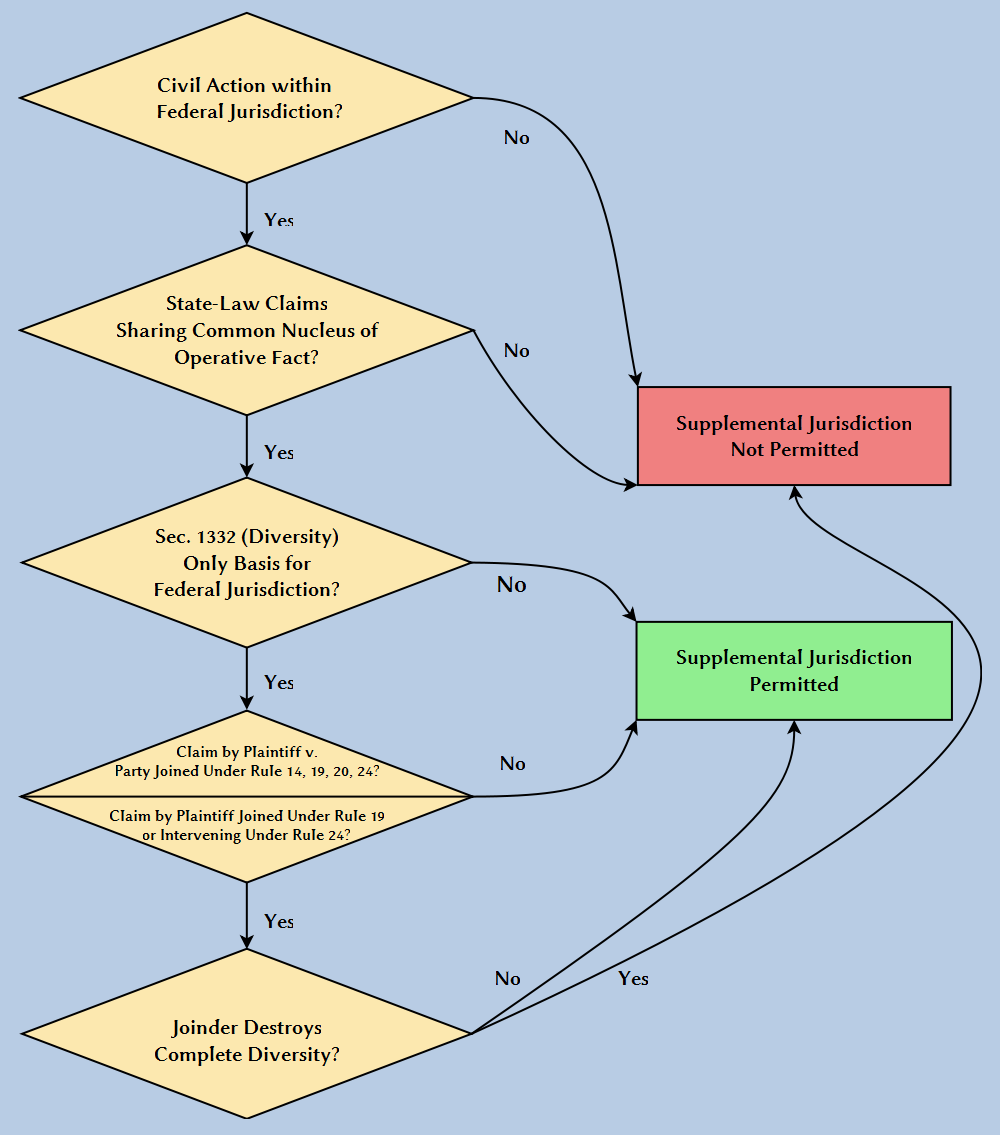
\includegraphics[width=0.9\linewidth,height=\textheight,keepaspectratio]{../img/1367.png}

}

\caption{Supplemental Jurisdiction Analysis}

\end{figure}%

\section{Removal}\label{removal}

Sometimes a plaintiff will file a suit in state court, even though a
federal court would also have subject matter jurisdiction over the
claims asserted. In such cases, the defendant may be able to remove the
suit to federal court. The conditions and procedures for removal are
govened by federal statute.

\subsection{28 U.S.C. § 1441}\label{u.s.c.-1441}

\subsubsection{Removal of civil actions}\label{removal-of-civil-actions}

(a) Except as otherwise expressly provided by Act of Congress, any civil
action brought in a State court of which the district courts of the
United States have original jurisdiction, may be removed by the
defendant or the defendants, to the district court of the United States
for the district and division embracing the place where such action is
pending \ldots.

(b) Any civil action of which the district courts have original
jurisdiction founded on a claim or right arising under the Constitution,
treaties or law of the United States, shall be removable without regard
to the citizenship or residence of the parties. Any other such action
shall be removable only if none of the parties in interest properly
joined and served as defendants is a citizen of the State in which such
action is brought.

\subsection{28 U.S.C. § 1445}\label{u.s.c.-1445}

\subsubsection{Nonremovable actions}\label{nonremovable-actions}

(a) A civil action in any State court against a railroad or its
receivers or trustees, arising under sections 1--4 and 5--10 of the Act
of April 22, 1908 (45 U.S.C.§51--54, 55--60), may not be removed to any
district court of the United States.

(b) A civil action in any State court against a carrier or its receivers
or trustees to recover damages for delay, loss, or injury of shipments,
arising under section 11706 or 14706 of title 49, may not be removed to
any district court of the United States unless the matter in controversy
exceeds \$10,000, exclusive of interest and costs.

(c) A civil action in any State court arising under the workmen's
compensation laws of such State may not be removed to any district court
of the United States.

(d) A civil action in any State court arising under section 40302 of the
Violence Against Women Act of 1994 may not be removed to any district
court of the United States.

\subsection{Note on § 1445}\label{note-on-1445}

Interestingly, of the four types of action that are not removable, three
involve suits arising under federal statutes. 45 U.S.C. §56; 49 U.S.C.
§11706(d)(1); 34 U.S.C, §12361(e)(3). Those statutes expressly allow
suits to be brought in either federal or state court. But, if the
plaintiff sues in state court, the defendant may not remove, even though
the federal court would have original jurisdiction under §1331.

In \emph{U.S. v. Morrison}, 529 U.S. 598 (2000), the Supreme Court
struck down section 40302 of the Violence Against Women Act, holding
that Congress lacked constitutional authority to establish a federal
cause of action for victims of crimes of violence motivated by gender.
Consequently, § 1445(d) is now moot.

\subsection{28 U.S.C. § 1447}\label{u.s.c.-1447}

\subsubsection{Procedure after removal
generally}\label{procedure-after-removal-generally}

(a) In any case removed from a State court, the district court may issue
all necessary orders and process to bring before it all proper parties
whether served by process issued by the State court or otherwise.

(b) It may require the removing party to file with its clerk copies of
all records and proceedings in such State court or may cause the same to
be brought before it by writ of certiorari issued to such State court.

(c) A motion to remand the case on the basis of any defect other than
lack of subject matter jurisdiction must be made within 30 days after
the filing of the notice of removal under section 1446(a). If at any
time before final judgment it appears that the district court lacks
subject matter jurisdiction, the case shall be remanded. An order
remanding the case may require payment of just costs and any actual
expenses, including attorney fees, incurred as a result of the removal.
A certified copy of the order of remand shall be mailed by the clerk to
the clerk of the State court. The State court may thereupon proceed with
such case.

(d) An order remanding a case to the State court from which it was
removed is not reviewable on appeal or otherwise, except that an order
remanding a case to the State court from which it was removed pursuant
to section 1442 or 1443 of this title shall be reviewable by appeal or
otherwise.

(e) If after removal the plaintiff seeks to join additional defendants
whose joinder would destroy subject matter jurisdiction, the court may
deny joinder, or permit joinder and remand the action to the State
court.

Note that removal is a one-way street. If a plaintiff files a suit in
federal court, the defendant may not ``remove'' or ``remand'' the case
to state court. The only option is to move for dismissal for lack of
federal subject matter jurisdiction (Fed. R. Civ. P. Rule 12(b)(1)).
Such dismissals are usually ``without prejudice'', meaning the plaintiff
may refile the suit in state court. If federal subject matter
jurisdiction is satisfied, the case remains in federal court.

\section{Review Questions}\label{review-questions-2}

\subsubsection{Question 1}\label{question-1-1}

Peter, a lifelong resident of Pennsylvania, worked as a delivery driver
in Pennsylvania for Dreadful Express Corp.~(DreadEx), which is
incorporated and has its corporate headquarters in Pennsylvania. When
Peter retired, he bought a second home in Florida, where he spends most
of the year, returning to Pennsylvania for the summers. DreadEx owes
Peter \$80,000 in commissions earned during his final year of work. When
the company fails to pay, Peter sues for breach of contract, filing his
claim in the U.S. District Court for the Eastern District of
Pennsylvania.

\emph{Does the court have subject-matter jurisdiction?}

\subsubsection{Question 2}\label{question-2-1}

Pam, a lifelong resident of North Carolina, files a products liability
action seeking \$150,000 in damages against Danger Corp.~in the U.S.
District Court for the Middle District of North Carolina. Danger is
incorporated in Delaware, has its sole manufacturing \& distribution
facility is in South Carolina, and its corporate offices (where all
significant business decisions are made) in North Carolina.

\emph{Does the court have subject-matter jurisdiction?}

\subsubsection{Question 3}\label{question-3-1}

Tri-State Landscaping, based in Johnson City, Tennessee, is organized as
an unincorporated business partnership under Tennessee law. Of
Tri-State's three partners, two are lifelong residents of Tennessee, the
other a lifelong resident of North Carolina. The company provides
residential and commercial landscaping services in eastern Tennessee,
southwestern Virginia, and northwestern North Carolina. Pat, a lifelong
resident of Virginia, hires Tri-State to maintain the lawn and garden at
her Abingdon, Virginia home. Dissatisfied with the work, Pat sues
Tri-State for breach of contract, filing the action in the U.S. District
Court for the Western District of Virginia. As permitted under the
applicable state law, Pat names Tri-State itself (not the individual
partners) as the sole defendant.

\emph{Does the court has subject-matter jurisdiction?}

\subsubsection{Question 4}\label{question-4-1}

Eleanor (domiciled in the state of Keystone) is employed by Bombco,
Inc.~(``Bombco''), a munitions manufacturer (incorporated in Delaware
with its sole place of business in Keystone). Bombco sells most of its
products to the U.S. Defense Department for use by the U.S. military.

During her first six months of work, Eleanor has been paid at the rate
of \$20/hour. She recently learned that a federal law, the Defense
Contractor Wage Fairness Act (``DCWFA''), requires federal defense
contractors to pay all employees at a rate no less than the ``local
prevailing wage'' for employees in the same job classification under the
U.S. Department of Labor's ``Standard Occupational Classification''
(``SOC'') system. Eleanor believes that her job falls within the SOC
classification for ``Engineering Technicians'', for which the ``local
prevailing wage'' under the DCWFA is \$25/hour.

Believing that she has been underpaid, Eleanor decides to sue Bombco for
\$4800 (representing the alleged underpayment of \$5/hour for the 960
hours she worked during the six month period). The DCWFA does not
provide for a private right of action for employees who believe they
have not been paid at the applicable prevailing wage rate. Instead,
Eleanor asserts a claim under the state Wage Payment \& Collection Law
(``WPCL''), which provides that an employer must pay all wages earned by
employees on regularly scheduled paydays. The WPCL also provides than an
employee may bring a civil lawsuit to collect any unpaid wages. A
plaintiff suing under the WPCL must allege and prove the following:

\begin{enumerate}
\def\labelenumi{\arabic{enumi}.}
\tightlist
\item
  The applicable rate of pay for the period subject to the suit,\\
\item
  The total amount of wages earned during the same period, and
\item
  The total amount of alleged underpayment during the same period.
\end{enumerate}

The Keystone Supreme Court has held that a WPCL plaintiff may satisfy
the first requirement by offering evidence of a wage rate imposed by
state or federal law.

Bombco disputes Eleanor's wage claim on two grounds. First, Bombco
contends that the Defense Contractor Wage Fairness Act does not apply to
Eleanor's job. Second, Bombco contends that, even if the DCWFA does
apply, the proper SOC classification for Eleanor's job is ``Cutting
Machine Operators, Metal \& Plastic'', for which the local prevailing
wage is only \$20/hour.

\emph{Does a federal court have subject-matter jurisdiction over
Eleanor's suit?}

\chapter{Choice of Governing Law}\label{choice-of-governing-law}

\section{The Rules of Decision Act}\label{the-rules-of-decision-act}

\subsection{The Rules of Decision Act, 28 U.S.C. §
1652}\label{the-rules-of-decision-act-28-u.s.c.-1652}

\subsubsection{State laws as rules of
decision}\label{state-laws-as-rules-of-decision}

The laws of the several states, except where the Constitution or
treaties of the United States or Acts of Congress otherwise require or
provide, shall be regarded as rules of decision in civil actions in the
courts of the United States, in cases where they apply.

\subsection{Note: ``The Laws of the Several
States''}\label{note-the-laws-of-the-several-states}

The Rules of Decision Act applies to cases in which federal courts hear
claims that arise under state law, i.e.~under diversity jurisdiction.
Federal courts must apply ``the laws of the several states'' as the
``rules of decision'' in such cases. By ``rules of decision'', the
statute means the substantive legal rules governing the claims,
i.e.~rules that define the rights, duties, and liabilities of the
parties. But what does the statute mean by ``laws of the several
states''?

\subsection{Swift v. Tyson (U.S. 1842)}\label{swift-v.-tyson-u.s.-1842}

{[}\textbf{Summary of Facts.} {\marginnote{\begin{footnotesize}A bill of
exchange \ldots{} is a signed, unconditional, written order binding one
party to pay a fixed sum of money to another party on demand or at a
predetermined date.''
\href{https://www.law.cornell.edu/wex/bill_of_exchange}{Wex Legal
Dictionary}\end{footnotesize}}} \emph{George Tyson purchased some land
from Nathaniel Norton and Jairus Keith. As partial payment, Tyson gave
Norton and Keith a bill of exchange. It turned out that, not only was
the land virtually worthless, North and Keith did not actually own it.
Before the bill of exchange came due, Norton signed it over to the
plaintiff, John Swift, ostensibly in payment of a debt. Swift then
sought payment on the bill of exchange from Tyson, who refused on the
ground that it was procured by fraud. Swift (a resident of Maine) sued
Tyson (a resident of New York) in federal court, which had jurisdiction
based on diversity of citizenship.}{]}

\subsubsection{Justice Story delivered the opinion of the
Court.}\label{justice-story-delivered-the-opinion-of-the-court.}

There is no doubt, that a bonâ fide holder of a negotiable instrument
for a valuable consideration, without any notice of facts which impeach
its validity as between the antecedent parties, if he takes it under an
endorsement made before the same becomes due, holds the title unaffected
by these facts, and may recover thereon, although as between the
antecedent parties the transaction may be without any legal validity.
This is a doctrine so long and so well established, and so essential to
the security of negotiable paper, that it is laid up among the
fundamentals of the law, and requires no authority or reasoning to be
now brought in its support. As little doubt is there, that the holder of
any negotiable paper, before it is due, is not bound to prove that he is
a bonâ fide holder for a valuable consideration, without notice; for the
law will presume that, in the absence of all rebutting proofs, and
therefore it is incumbent upon the defendant to establish by way of
defence satisfactory proofs of the contrary, and thus to overcome the
primâ facie title of the plaintiff.

In the present case, the plaintiff is a bonâ fide holder without notice
for what the law deems a good and valid consideration, that is, for a
pre-existing debt; and the only real question in the cause is, whether,
under the circumstances of the present case, such a pre-existing debt
constitutes a valuable consideration in the sense of the general rule
applicable to negotiable instruments. We say, under the circumstances of
the present case, for the acceptance having been made in New York, the
argument on behalf of the defendant is, that the contract is to be
treated as a New York contract, and therefore to be governed by the laws
of New York, as expounded by its Courts, as well upon general
principles, as by the express provisions of the {[}Rules of Decision
Act{]}. And then it is further contended, that by the law of New York,
as thus expounded by its Courts, a pre-existing debt does not
constitute, in the sense of the general rule, a valuable consideration
applicable to negotiable instruments.

But, admitting the doctrine to be fully settled in New York, it remains
to be considered, whether it is obligatory upon this Court, if it
differs from the principles established in the general commercial law.
It is observable that the Courts of New York do not found their
decisions upon this point upon any local statute, or positive, fixed, or
ancient local usage: but they deduce the doctrine from the general
principles of commercial law. It is, however, contended, that the
{[}Rules of Decision Act{]} furnishes a rule obligatory upon this Court
to follow the decisions of the state tribunals in all cases to which
they apply. That section provides ``that the laws of the several states,
except where the Constitution, treaties, or statutes of the United
States shall otherwise require or provide, shall be regarded as rules of
decision in trials at common law in the Courts of the United States, in
cases where they apply.'' In order to maintain the argument, it is
essential, therefore, to hold, that the word ``laws,'' in this section,
includes within the scope of its meaning the decisions of the local
tribunals. In the ordinary use of language it will hardly be contended
that the decisions of Courts constitute laws. They are, at most, only
evidence of what the laws are; and are not of themselves laws. They are
often re-examined, reversed, and qualified by the Courts themselves,
whenever they are found to be either defective, or ill-founded, or
otherwise incorrect. The laws of a state are more usually understood to
mean the rules and enactments promulgated by the legislative authority
thereof, or long established local customs having the force of laws. In
all the various cases which have hitherto come before us for decision,
this Court have uniformly supposed, that the true interpretation of the
thirty-fourth section limited its application to state laws strictly
local, that is to say, to the positive statutes of the state, and the
construction thereof adopted by the local tribunals, and to rights and
titles to things having a permanent locality, such as the rights and
titles to real estate, and other matters immovable and intraterritorial
in their nature and character. It never has been supposed by us, that
the section did apply, or was designed to apply, to questions of a more
general nature, not at all dependent upon local statutes or local usages
of a fixed and permanent operation, as, for example, to the construction
of ordinary contracts or other written instruments, and especially to
questions of general commercial law, where the state tribunals are
called upon to perform the like functions as ourselves, that is, to
ascertain upon general reasoning and legal analogies, what is the true
exposition of the contract or instrument, or what is the just rule
furnished by the principles of commercial law to govern the case. And we
have not now the slightest difficulty in holding, that this section,
upon its true intendment and construction, is strictly limited to local
statutes and local usages of the character before stated, and does not
extend to contracts and other instruments of a commercial nature, the
true interpretation and effect whereof are to be sought, not in the
decisions of the local tribunals, but in the general principles and
doctrines of commercial jurisprudence. Undoubtedly, the decisions of the
local tribunals upon such subjects are entitled to, and will receive,
the most deliberate attention and respect of this Court; but they cannot
furnish positive rules, or conclusive authority, by which our own
judgments are to be bound up and governed.
{\marginnote{\begin{footnotesize}``There will not be different laws at
Rome and at Athens, or different laws now and in the future, but one
eternal and unchangeable law will be valid for all nations and all
times''.\end{footnotesize}}} The law respecting negotiable instruments
may be truly declared in the language of Cicero, to be in a great
measure, not the law of a single country only, but of the commercial
world. \emph{Non erit alia lex Romæ, alia Athenis, alia nunc, alia
posthac, sed et apud omnes gentes, et omni tempore, una eademque lex
obtenebit}.

It becomes necessary for us, therefore, upon the present occasion to
express our own opinion of the true result of the commercial law upon
the question now before us. And we have no hesitation in saying, that a
pre-existing debt does constitute a valuable consideration in the sense
of the general rule already stated, as applicable to negotiable
instruments. Assuming it to be true, (which, however, may well admit of
some doubt from the generality of the language,) that the holder of a
negotiable instrument is unaffected with the equities between the
antecedent parties, of which he has no notice, only where he receives it
in the usual course of trade and business for a valuable consideration,
before it becomes due; we are prepared to say, that receiving it in
payment of, or as security for a pre-existing debt, is according to the
known usual course of trade and business.

\subsection{\texorpdfstring{Note: \emph{Swift} and Its
Discontents}{Note: Swift and Its Discontents}}\label{note-swift-and-its-discontents}

Justice Story's opinion quotes the Roman statesman and philosopher
Cicero for the proposition that the common law cannot differ from state
to state. The cited passage\footnote{Cicero, On the Republic, Book III,
  §22} summarizes the natural law paradigm:

\begin{quote}
True law is right reason in agreement with nature; it is of universal
application, unchanging and everlasting; It is a sin to try to alter
this law, nor is it allowable to attempt to repeal any part of it, and
it is impossible to abolish it entirely. We cannot be freed from its
obligations by senate or people, and we need not look outside ourselves
for an expounder or interpreter of it. And there will not be different
laws at Rome and at Athens, or different laws now and in the future, but
one eternal and unchangeable law will be valid for all nations and all
times, and there will be one master and ruler, that is, God, over us
all, for he is the author of this law, its promulgator, and its
enforcing judge. Whoever is disobedient is fleeing from himself and
denying his human nature, and by reason of this very fact he will suffer
the worst penalties, even if he escapes what is commonly considered
punishment.
\end{quote}

During the late 19th and early 20th centuries, the legal field
experienced a paradigm shift,\footnote{A paradigm shift is a
  transformation in the fundamental assumptions, theories, and practice
  of a scientific or professional community. ``When the transition is
  completed, the profession will have changed its view of the field, its
  methods, and its goals.'' Kuhn \& Hacking (2012): 84-85.} with
concepts and methods associated with legal
\href{https://plato.stanford.edu/archives/fall2009/entries/legal-positivism/}{positivism},
\href{https://lsolum.typepad.com/legal_theory_lexicon/2006/09/legal_theory_le_2.html}{realism},
and
\href{https://lsolum.typepad.com/legaltheory/2018/07/legal-theory-lexicon-pragmatism.html}{pragmatism}
challenging the previously dominant paradigm of natural law and
formalism. Cases like \emph{Erie} and \emph{International Shoe}, along
with the adoption of the Federal Rules of Civil Procedure, were
significant moments in this jurisprudential revolution.\footnote{See,
  e.g.~Rutherglen (2001); Sawyer III (2001); Marcus (2009); Casto
  (1987).}

Among those leading the charge was Oliver Wendell Holmes, Jr., whose
work as a legal scholar and opinions as a Supreme Court Justice advanced
a positivist understanding of law and pragmatist approach to judicial
decision-making, and laid the groundwork for overturning \emph{Swift}.

Oliver Wendall Holmes, \emph{The Common Law} (1881):

\begin{quote}
The life of the law has not been logic: it has been experience. The felt
necessities of the time, the prevalent moral and political theories,
intuitions of public policy, avowed or unconscious, even the prejudices
which judges share with their fellow-men, have had a good deal more to
do than the syllogism in determining the rules by which men should be
governed. The law embodies the story of a nation's development through
many centuries, and it cannot be dealt with as if it contained only the
axioms and corollaries of a book of mathematics. In order to know what
it is, we must know what it has been, and what it tends to become. We
must alternately consult history and existing theories of legislation.
But the most difficult labor will be to understand the combination of
the two into new products at every stage. The substance of the law at
any given time pretty nearly corresponds, so far as it goes, with what
is then understood to be convenient; but its form and machinery, and the
degree to which it is able to work out desired results, depend very much
upon its past.
\end{quote}

\emph{Southern Pacific Co.~v. Jensen}, 244 U.S. 205 (1917) (Holmes, J.
dissenting):

\begin{quote}
The common law is not a brooding omnipresence in the sky but the
articulate voice of some sovereign or quasi-sovereign that can be
identified; although some decisions with which I have disagreed seem to
me to have forgotten the fact. It always is the law of some State.
\end{quote}

\emph{Kuhn v. Fairmont Coal Co.}, 215 US 349, 370-372 (1910) (Holmes,
J., dissenting):

\begin{quote}
I admit that plenty of language can be found in the earlier cases to
support the present decision. That is not surprising in view of the
uncertainty and vacillation of the theory upon which \emph{Swift v.
Tyson}, and the later extensions of its doctrine have proceeded. But I
suppose it will be admitted on the other side that even the independent
jurisdiction of the Circuit Courts of the United States is a
jurisdiction only to declare the law, at least in a case like the
present, and only to declare the law of the State. It is not an
authority to make it. \emph{Swift v. Tyson} was justified on the ground
that that was all that the state courts did. But as has been pointed out
by a recent accomplished and able writer, that fiction had to be
abandoned and was abandoned when this court came to decide the municipal
bond cases, beginning with \emph{Gelpcke v. Dubuque}. In those cases the
court recognized the fact that decisions of state courts of last resort
make law for the State. The principle is that a change of judicial
decision after a contract has been made on the faith of an earlier one
the other way is a change of the law.

The cases of the class to which I refer have not stood on the ground
that this court agreed with the first decision, but on the ground that
the state decision made the law for the State, and therefore should be
given only a prospective operation when contracts had been entered into
under the law as earlier declared. In various instances this court has
changed its decision or rendered different decisions on similar facts
arising in different States in order to conform to what is recognized as
the local law.

Whether \emph{Swift v. Tyson} can be reconciled with \emph{Gelpcke v.
Dubuque}, I do not care to enquire. I assume both cases to represent
settled doctrines, whether reconcilable or not. But the moment you leave
those principles which it is desirable to make uniform throughout the
United States and which the decisions of this court tend to make
uniform, obviously it is most undesirable for the courts of the United
States to appear as interjecting an occasional arbitrary exception to a
rule that in every other case prevails. I never yet have heard a
statement of any reason justifying the power, and I find it hard to
imagine one. I know of no authority in this court to say that in general
state decisions shall make law only for the future. Judicial decisions
have had retrospective operation for near a thousand years. It is said
that we must exercise our independent judgment --- but as to what?
Surely as to the law of the States. Whence does that law issue?
Certainly not from us. But it does issue and has been recognized by this
court as issuing from the state courts as well as from the state
legislatures. When we know what the source of the law has said that it
shall be, our authority is at an end. The law of a State does not become
something outside of the state court and independent of it by being
called the common law. Whatever it is called it is the law as declared
by the state judges and nothing else.

If, as I believe, my reasoning is correct, it justifies our stopping
when we come to a kind of case that by nature and necessity is
peculiarly local, and one as to which the latest intimations and indeed
decisions of this court are wholly in accord with what I think to be
sound law. To administer a different law is ``to introduce into the
jurisprudence of the State of Illinois the discordant elements of a
substantial right which is protected in one set of courts and denied in
the other, with no superior to decide which is right.'' It is admitted
that we are bound by a settled course of decisions, irrespective of
contract, because they make the law. I see no reason why we are less
bound by a single one.
\end{quote}

\emph{Black \& White Taxicab Co.~v. Brown \& Yellow Taxicab Co.}, 279
U.S. 518, 532-536 (1928) (Holmes, J., dissenting):

\begin{quote}
This is a suit brought by The Brown and Yellow Taxicab and Transfer
Company, as plaintiff, to prevent The Black and White Taxicab and
Transfer Company, from interfering with the carrying out of a contract
between the plaintiff and the other defendant, The Louisville and
Nashville Railroad Company. The Circuit Court of Appeals, affirming a
decree of the District Court, granted an injunction and upheld this
contract. It expressly recognized that the decisions of the Kentucky
Courts held that in Kentucky a railroad company could not grant such
rights, but this being a `question of general law' it went its own way
regardless of the Courts of this State.

The Circuit Court of Appeals had so considerable a tradition behind it
in deciding as it did that if I did not regard the case as exceptional I
should not feel warranted in presenting my own convictions again after
having stated them in \emph{Kuhn v. Fairmont Coal Company}. But the
question is important and in my opinion the prevailing doctrine has been
accepted upon a subtle fallacy that never has been analyzed. If I am
right the fallacy has resulted in an unconstitutional assumption of
powers by the Courts of the United States which no lapse of time or
respectable array of opinion should make us hesitate to correct.
Therefore I think it proper to state what I think the fallacy is. ---
The often repeated proposition of this and the lower Courts is that the
parties are entitled to an independent judgment on matters of general
law. By that phrase is meant matters that are not governed by any law of
the United States or by any statute of the State --- matters that in
States other than Louisiana are governed in most respects by what is
called the common law. It is through this phrase that what I think the
fallacy comes in.

Books written about any branch of the common law treat it as a unit,
cite cases from this Court, from the Circuit Courts of Appeals, from the
State Courts, from England and the Colonies of England indiscriminately,
and criticize them as right or wrong according to the writer's notions
of a single theory. It is very hard to resist the impression that there
is one august corpus, to understand which clearly is the only task of
any Court concerned. If there were such a transcendental body of law
outside of any particular State but obligatory within it unless and
until changed by statute, the Courts of the United States might be right
in using their independent judgment as to what it was. But there is no
such body of law. The fallacy and illusion that I think exist consist in
supposing that there is this outside thing to be found. Law is a word
used with different meanings, but law in the sense in which courts speak
of it today does not exist without some definite authority behind it.
The common law so far as it is enforced in a State, whether called
common law or not, is not the common law generally but the law of that
State existing by the authority of that State without regard to what it
may have been in England or anywhere else. It may be adopted by statute
in place of another system previously in force. But a general adoption
of it does not prevent the State Courts from refusing to follow the
English decisions upon a matter where the local conditions are
different. It may be changed by statute, as is done every day. It may be
departed from deliberately by judicial decisions, as with regard to
water rights, in States where the common law generally prevails.
Louisiana is a living proof that it need not be adopted at all. Whether
and how far and in what sense a rule shall be adopted whether called
common law or Kentucky law is for the State alone to decide.

If within the limits of the Constitution a State should declare one of
the disputed rules of general law by statute there would be no doubt of
the duty of all Courts to bow, whatever their private opinions might be.
I see no reason why it should have less effect when it speaks by its
other voice. If a state constitution should declare that on all matters
of general law the decisions of the highest Court should establish the
law until modified by statute or by a later decision of the same Court,
I do not perceive how it would be possible for a Court of the United
States to refuse to follow what the State Court decided in that domain.
But when the constitution of a State establishes a Supreme Court it by
implication does make that declaration as clearly as if it had said it
in express words, so far as it is not interfered with by the superior
power of the United States. The Supreme Court of a State does something
more than make a scientific inquiry into a fact outside of and
independent of it. It says, with an authority that no one denies, except
when a citizen of another State is able to invoke an exceptional
jurisdiction, that thus the law is and shall be. Whether it be said to
make or to declare the law, it deals with the law of the State with
equal authority however its function may be described.

Mr.~Justice Story in \emph{Swift v. Tyson}, evidently under the tacit
domination of the fallacy to which I have referred, devotes some energy
to showing that \hyperref[the-rules-of-decision-act]{the Rules of
Decision Act} refers only to statutes when it provides that except as
excepted the laws of the several States shall be regarded as rules of
decision in trials at common law in Courts of the United States. An
examination of the original document by a most competent hand has shown
that Mr.~Justice Story probably was wrong if anyone is interested to
inquire what the framers of the instrument meant. 37 Harvard Law Review,
49, at pp.~81-88. But this question is deeper than that; it is a
question of the authority by which certain particular acts, here the
grant of exclusive privileges in a railroad station, are governed. In my
opinion the authority and only authority is the State, and if that be
so, the voice adopted by the State as its own should utter the last
word. I should leave \emph{Swift v. Tyson} undisturbed, as I indicated
in \emph{Kuhn v. Fairmont Coal Co.}, but I would not allow it to spread
the assumed dominion into new fields.

In view of what I have said it is not necessary for me to give
subordinate and narrower reasons for my opinion that the decision below
should be reversed. But there are adequate reasons short of what I think
should be recognized. This is a question concerning the lawful use of
land in Kentucky by a corporation chartered by Kentucky. The policy of
Kentucky with regard to it has been settled in Kentucky for more than
thirty-five years. Even under the rule that I combat, it has been
recognized that a settled line of state decisions was conclusive to
establish a rule of property or the public policy of the State. I should
have supposed that what arrangements could or could not be made for the
use of a piece of land was a purely local question, on which, if on
anything, the State should have its own way and the State Courts should
be taken to declare what the State wills.
\end{quote}

Holmes stepped down from the Court in 1932 and died in 1935. Three years
later, the Court, in an opinion by Justice Louis Brandeis (another
important figure in legal pragmatism and realism) overturned
\emph{Swift} and adopted a positivist interpretation of the Rules of
Decision Act.

\subsection{Erie R. Co.~v. Tompkins (U.S.
1938)}\label{erie-r.-co.-v.-tompkins-u.s.-1938}

\subsubsection{Justice Brandeis delivered the opinion of the
Court.}\label{justice-brandeis-delivered-the-opinion-of-the-court.}

The question for decision is whether the oft-challenged doctrine of
\emph{Swift v. Tyson} shall now be disapproved.

Tompkins, a citizen of Pennsylvania, was injured on a dark night by a
passing freight train of the Erie Railroad Company while walking along
its right of way at Hughestown in that State. He claimed that the
accident occurred through negligence in the operation, or maintenance,
of the train; that he was rightfully on the premises as licensee because
on a commonly used beaten footpath which ran for a short distance
alongside the tracks; and that he was struck by something which looked
like a door projecting from one of the moving cars. To enforce that
claim he brought an action in the federal court for southern New York,
which had jurisdiction because the company is a corporation of that
State. It denied liability; and the case was tried by a jury.

The Erie insisted that its duty to Tompkins was no greater than that
owed to a trespasser. It contended, among other things, that its duty to
Tompkins, and hence its liability, should be determined in accordance
with the Pennsylvania law; that under the law of Pennsylvania, as
declared by its highest court, persons who use pathways along the
railroad right of way---that is a longitudinal pathway as distinguished
from a crossing---are to be deemed trespassers; and that the railroad is
not liable for injuries to undiscovered trespassers resulting from its
negligence, unless it be wanton or wilful. Tompkins denied that any such
rule had been established by the decisions of the Pennsylvania courts;
and contended that, since there was no statute of the State on the
subject, the railroad's duty and liability is to be determined in
federal courts as a matter of general law.

The trial judge refused to rule that the applicable law precluded
recovery. The jury brought in a verdict of \$30,000; and the judgment
entered thereon was affirmed by the Circuit Court of Appeals, which held
that it was unnecessary to consider whether the law of Pennsylvania was
as contended, because the question was one not of local, but of general,
law and that ``upon questions of general law the federal courts are
free, in the absence of a local statute, to exercise their independent
judgment as to what the law is; and it is well settled that the question
of the responsibility of a railroad for injuries caused by its servants
is one of general law. Where the public has made open and notorious use
of a railroad right of way for a long period of time and without
objection, the company owes to persons on such permissive pathway a duty
of care in the operation of its trains. It is likewise generally
recognized law that a jury may find that negligence exists toward a
pedestrian using a permissive path on the railroad right of way if he is
hit by some object projecting from the side of the train.''

The Erie had contended that application of the Pennsylvania rule was
required, among other things, by
\hyperref[the-rules-of-decision-act]{the Rules of Decision Act}, which
provides:

\begin{quote}
The laws of the several States, except where the Constitution, treaties,
or statutes of the United States otherwise require or provide, shall be
regarded as rules of decision in trials at common law, in the courts of
the United States, in cases where they apply.
\end{quote}

Because of the importance of the question whether the federal court was
free to disregard the alleged rule of the Pennsylvania common law, we
granted certiorari.

\emph{First}. \emph{Swift v. Tyson} held that federal courts exercising
jurisdiction on the ground of diversity of citizenship need not, in
matters of general jurisprudence, apply the unwritten law of the State
as declared by its highest court; that they are free to exercise an
independent judgment as to what the common law of the State is---or
should be; and that, as there stated by Mr.~Justice Story:

\begin{quote}
the true interpretation of the thirty-fourth section limited its
application to state laws strictly local, that is to say, to the
positive statutes of the state, and the construction thereof adopted by
the local tribunals, and to rights and titles to things having a
permanent locality, such as the rights and titles to real estate, and
other matters immovable and intraterritorial in their nature and
character. It never has been supposed by us, that the section did apply,
or was intended to apply, to questions of a more general nature, not at
all dependent upon local statutes or local usages of a fixed and
permanent operation, as, for example, to the construction of ordinary
contracts or other written instruments, and especially to questions of
general commercial law, where the state tribunals are called upon to
perform the like functions as ourselves, that is, to ascertain upon
general reasoning and legal analogies, what is the true exposition of
the contract or instrument, or what is the just rule furnished by the
principles of commercial law to govern the case.
\end{quote}

The Court in applying \hyperref[the-rules-of-decision-act]{the Rules of
Decision Act} to equity cases, in \emph{Mason v. United States}, 260
U.S. 545, 559, said: ``The statute, however, is merely declarative of
the rule which would exist in the absence of the statute.'' The federal
courts assumed, in the broad field of ``general law,'' the power to
declare rules of decision which Congress was confessedly without power
to enact as statutes. Doubt was repeatedly expressed as to the
correctness of the construction given
\hyperref[the-rules-of-decision-act]{the Rules of Decision Act}, and as
to the soundness of the rule which it introduced. But it was the more
recent research of a competent scholar, who examined the original
document, which established that the construction given to it by the
Court was erroneous; and that the purpose of the section was merely to
make certain that, in all matters except those in which some federal law
is controlling, the federal courts exercising jurisdiction in diversity
of citizenship cases would apply as their rules of decision the law of
the State, unwritten as well as written.\footnote{(n.5 in opinion)
  Charles Warren, New Light on the History of the Federal Judiciary Act
  of 1789 (1923) 37 Harv. L. Rev.~49, 51-52, 81-88, 108.}

Criticism of the doctrine became widespread after the decision of
\emph{Black \& White Taxicab Co.~v. Brown \& Yellow Taxicab Co.}, 276
U.S. 518 (1928). There, Brown and Yellow, a Kentucky corporation owned
by Kentuckians, and the Louisville and Nashville Railroad, also a
Kentucky corporation, wished that the former should have the exclusive
privilege of soliciting passenger and baggage transportation at the
Bowling Green, Kentucky, railroad station; and that the Black and White,
a competing Kentucky corporation, should be prevented from interfering
with that privilege. Knowing that such a contract would be void under
the common law of Kentucky, it was arranged that the Brown and Yellow
reincorporate under the law of Tennessee, and that the contract with the
railroad should be executed there. The suit was then brought by the
Tennessee corporation in the federal court for western Kentucky to
enjoin competition by the Black and White; an injunction issued by the
District Court was sustained by the Court of Appeals; and this Court,
citing many decisions in which the doctrine of \emph{Swift v. Tyson} had
been applied, affirmed the decree.

\emph{Second}. Experience in applying the doctrine of \emph{Swift v.
Tyson}, had revealed its defects, political and social; and the benefits
expected to flow from the rule did not accrue. Persistence of state
courts in their own opinions on questions of common law prevented
uniformity; and the impossibility of discovering a satisfactory line of
demarcation between the province of general law and that of local law
developed a new well of uncertainties.

On the other hand, the mischievous results of the doctrine had become
apparent. Diversity of citizenship jurisdiction was conferred in order
to prevent apprehended discrimination in state courts against those not
citizens of the State. \emph{Swift v. Tyson} introduced grave
discrimination by non-citizens against citizens. It made rights enjoyed
under the unwritten ``general law'' vary according to whether
enforcement was sought in the state or in the federal court; and the
privilege of selecting the court in which the right should be determined
was conferred upon the non-citizen. Thus, the doctrine rendered
impossible equal protection of the law. In attempting to promote
uniformity of law throughout the United States, the doctrine had
prevented uniformity in the administration of the law of the State.

The discrimination resulting became in practice far-reaching. This
resulted in part from the broad province accorded to the so-called
``general law'' as to which federal courts exercised an independent
judgment. In addition to questions of purely commercial law, ``general
law'' was held to include the obligations under contracts entered into
and to be performed within the State, the extent to which a carrier
operating within a State may stipulate for exemption from liability for
his own negligence or that of his employee; the liability for torts
committed within the State upon persons resident or property located
there, even where the question of liability depended upon the scope of a
property right conferred by the State; and the right to exemplary or
punitive damages. Furthermore, state decisions construing local deeds,
mineral conveyances, and even devises of real estate were disregarded.

In part the discrimination resulted from the wide range of persons held
entitled to avail themselves of the federal rule by resort to the
diversity of citizenship jurisdiction. Through this jurisdiction
individual citizens willing to remove from their own State and become
citizens of another might avail themselves of the federal rule. And,
without even change of residence, a corporate citizen of the State could
avail itself of the federal rule by re-incorporating under the laws of
another State, as was done in the \emph{Taxicab} case.

The injustice and confusion incident to the doctrine of \emph{Swift v.
Tyson} have been repeatedly urged as reasons for abolishing or limiting
diversity of citizenship jurisdiction. Other legislative relief has been
proposed. If only a question of statutory construction were involved, we
should not be prepared to abandon a doctrine so widely applied
throughout nearly a century. But the unconstitutionality of the course
pursued has now been made clear and compels us to do so.

\emph{Third}. Except in matters governed by the Federal Constitution or
by Acts of Congress, the law to be applied in any case is the law of the
State. And whether the law of the State shall be declared by its
Legislature in a statute or by its highest court in a decision is not a
matter of federal concern. There is no federal general common law.
Congress has no power to declare substantive rules of common law
applicable in a State whether they be local in their nature or
``general,'' be they commercial law or a part of the law of torts. And
no clause in the Constitution purports to confer such a power upon the
federal courts. As stated by Mr.~Justice Field when protesting in
\emph{Baltimore \& Ohio R. Co.~v. Baugh}, 149 U.S. 368, 401, against
ignoring the Ohio common law of fellow servant liability:

\begin{quote}
I am aware that what has been termed the general law of the
country---which is often little less than what the judge advancing the
doctrine thinks at the time should be the general law on a particular
subject---has been often advanced in judicial opinions of this court to
control a conflicting law of a State. I admit that learned judges have
fallen into the habit of repeating this doctrine as a convenient mode of
brushing aside the law of a State in conflict with their views. And I
confess that, moved and governed by the authority of the great names of
those judges, I have, myself, in many instances, unhesitatingly and
confidently, but I think now erroneously, repeated the same doctrine.
But, notwithstanding the great names which may be cited in favor of the
doctrine, and notwithstanding the frequency with which the doctrine has
been reiterated, there stands, as a perpetual protest against its
repetition, the Constitution of the United States, which recognizes and
preserves the autonomy and independence of the States---independence in
their legislative and independence in their judicial departments.
Supervision over either the legislative or the judicial action of the
States is in no case permissible except as to matters by the
Constitution specifically authorized or delegated to the United States.
Any interference with either, except as thus permitted, is an invasion
of the authority of the State and, to that extent, a denial of its
independence.
\end{quote}

The fallacy underlying the rule declared in \emph{Swift v. Tyson} is
made clear by Mr.~Justice Holmes. The doctrine rests upon the assumption
that there is ``a transcendental body of law outside of any particular
State but obligatory within it unless and until changed by statute,''
that federal courts have the power to use their judgment as to what the
rules of common law are; and that in the federal courts ``the parties
are entitled to an independent judgment on matters of general law'':

\begin{quote}
but law in the sense in which courts speak of it today does not exist
without some definite authority behind it. The common law so far as it
is enforced in a State, whether called common law or not, is not the
common law generally but the law of that State existing by the authority
of that State without regard to what it may have been in England or
anywhere else. ``the authority and only authority is the State, and if
that be so, the voice adopted by the State as its own {[}whether it be
of its Legislature or of its Supreme Court{]} should utter the last
word.''
\end{quote}

Thus the doctrine of \emph{Swift v. Tyson}, is, as Mr.~Justice Holmes
said, ``an unconstitutional assumption of powers by courts of the United
States which no lapse of time or respectable array of opinion should
make us hesitate to correct.'' In disapproving that doctrine we do not
hold unconstitutional §34 of the Federal Judiciary Act of 1789 or any
other Act of Congress. We merely declare that in applying the doctrine
this Court and the lower courts have invaded rights which in our opinion
are reserved by the Constitution to the several States.

\emph{Fourth}.{\marginnote{\begin{footnotesize}On remand, the
\href{https://scholar.google.com/scholar_case?case=15621582385726516928}{Court
of Appeals} concluded that, ``Under the Pennsylvania law, the defendant
owed no duty to the plaintiff except to refrain from wanton or wilful
injury.'' Because Tompkins neither alleged nor proved that the Railroad
acted wantonly or wilfully, the case was remanded to the trial court
with directions to enter judgment in favor of the Railroad. For a more
detailed account of the incident (including photos of Tompkins before
and after his unfortunate encounter with the train), see Frye
(2018)\end{footnotesize}}} The defendant contended that by the common
law of Pennsylvania as declared by its highest court, the only duty owed
to the plaintiff was to refrain from wilful or wanton injury. The
plaintiff denied that such is the Pennsylvania law. In support of their
respective contentions the parties discussed and cited many decisions of
the Supreme Court of the State. The Circuit Court of Appeals ruled that
the question of liability is one of general law; and on that ground
declined to decide the issue of state law. As we hold this was error,
the judgment is reversed and the case remanded to it for further
proceedings in conformity with our opinion.

\subsection{\texorpdfstring{Note: Substance and Procedure under
\emph{Erie}}{Note: Substance and Procedure under Erie}}\label{note-substance-and-procedure-under-erie}

The underlying issue in \emph{Erie} was one of substantive law: the
standard of care that the Railroad owed Tompkins. In a concurring
opinion, Justice Reed suggested that on matters of procedure, federal
courts were not bound to follow state law:

\begin{quote}
The line between procedural and substantive law is hazy but no one
doubts federal power over procedure. The Judiciary Article and the
``necessary and proper'' clause of Article One may fully authorize
legislation, such as this section of the Judiciary Act.
\end{quote}

In the aftermath of \emph{Erie}, the Court sought to provide an answer
to the question of how to draw the line between substance and procedure:

\paragraph{Guaranty Trust Co.~of New York v. York, 326 U.S. 99
(1945)}\label{guaranty-trust-co.-of-new-york-v.-york-326-u.s.-99-1945}

York sued Guaranty Trust for breach of fiduciary duty. The issue was
whether, ``in a suit brought on the equity side\footnote{``The term
  `equity' refers to a particular set of remedies and associated
  procedures involved with civil law. These equitable doctrines and
  procedures are distinguished from `legal' ones. While legal remedies
  typically involve monetary damages, equitable relief typically refers
  to injunctions, specific performance, or vacatur. A court will usually
  award equitable remedies when a legal remedy is insufficient or
  inadequate.'' \href{https://www.law.cornell.edu/wex/equity}{Wex Legal
  Dictionary} The Federal Rules of Civil Procedure eliminated the
  procedural distinction between ``law'' and ``equity'' suits, and most
  state judicial systems have followed suit.} of a federal district
court that court is required to apply the State statute of limitations
that would govern like suits in the courts of a State where the federal
court is sitting even though the exclusive basis of federal jurisdiction
is diversity of citizenship.'' If so, the suit would be dismissed as
untimely. This turned on whether application of the state statute of
limitations to bar ``a claim created by the States is a matter of
`substantive rights' to be respected by a federal court of equity when
that court's jurisdiction is dependent on the fact that there is a
State-created right, or is such statute of 'a mere remedial character,
which a federal court may disregard?''

Rather than mechanically applying the labels ``substance'' and
``procedure'', the Court took a pragmatic approach focused on whether
application of a different rule would yield a different outcome.

\begin{quote}
Here we are dealing with a right to recover derived not from the United
States but from one of the States. When, because the plaintiff happens
to be a non-resident, such a right is enforceable in a federal as well
as in a State court, the forms and mode of enforcing the right may at
times, naturally enough, vary because the two judicial systems are not
identic. But since a federal court adjudicating a State-created right
solely because of the diversity of citizenship of the parties is for
that purpose, in effect, only another court of the State, it cannot
afford recovery if the right to recover is made unavailable by the State
nor can it substantially affect the enforcement of the right as given by
the State.

And so the question is not whether a statute of limitations is deemed a
matter of ``procedure'' in some sense. The question is whether such a
statute concerns merely the manner and the means by which a right to
recover, as recognized by the State, is enforced, or whether such
statutory limitation is a matter of substance in the aspect that alone
is relevant to our problem, namely, does it significantly affect the
result of a litigation for a federal court to disregard a law of a State
that would be controlling in an action upon the same claim by the same
parties in a State court?

It is therefore immaterial whether statutes of limitation are
characterized either as ``substantive'' or ``procedural'' in State court
opinions in any use of those terms unrelated to the specific issue
before us. \emph{Erie R. Co.~v. Tompkins} was not an endeavor to
formulate scientific legal terminology. It expressed a policy that
touches vitally the proper distribution of judicial power between State
and federal courts. In essence, the intent of that decision was to
insure that, in all cases where a federal court is exercising
jurisdiction solely because of the diversity of citizenship of the
parties, the outcome of the litigation in the federal court should be
substantially the same, so far as legal rules determine the outcome of a
litigation, as it would be if tried in a State court. The nub of the
policy that underlies \emph{Erie R. Co.~v. Tompkins} is that for the
same transaction the accident of a suit by a non-resident litigant in a
federal court instead of in a State court a block away should not lead
to a substantially different result.

Plainly enough, a statute that would completely bar recovery in a suit
if brought in a State court bears on a State-created right vitally and
not merely formally or negligibly. As to consequences that so intimately
affect recovery or non-recovery a federal court in a diversity case
should follow State law.
\end{quote}

\paragraph{Ragan v. Merchants Transfer \& Warehouse Co., 337 U.S. 530
(1949)}\label{ragan-v.-merchants-transfer-warehouse-co.-337-u.s.-530-1949}

Ragan sued Merchants Transfer for injuries resulting from a traffic
accident. A two-year statute of limitations under state law applied. The
plaintiff filed the complaint in federal court less than two years after
the accident, but did not serve the complaint on the defendant until
more than two years had passed. Relying on Fed. R. Civ. P. Rule 3 (``A
civil action is commenced by filing a complaint with the court.''), the
plaintiff argued that filing the complaint was sufficient to satisfy the
statute of limitations. The defendant argued that the federal court must
follow state law, under which the statute of limitations was not
satisfied unless the suit was both filed and served within the allotted
time.

As in \emph{Guaranty Trust}, the Court focused on whether applying
different rules in state and federal court would yield different
outcomes. Once again, the Court held that the federal court must follow
state law, under which the plaintiff's right to relief would be
extinguished.

\paragraph{Woods v. Interstate Realty, 337 U.S. 535 (1949) and Cohen v.
Beneficial Indust. Loan Corp, 337 U.S. 541
(1949)}\label{woods-v.-interstate-realty-337-u.s.-535-1949-and-cohen-v.-beneficial-indust.-loan-corp-337-u.s.-541-1949}

In these two cases, decided together with \emph{Ragan}, the Court
likewise held that the federal court must apply state law rules where a
contrary federal rule would have yielded different outcomes. \emph{Woods
v. Interstate Realty} (State rule, barring unqualified business from
appearing in state court, applies in federal diversity action);
\emph{Cohen v. Beneficial Indust. Loan Corp}, (State rule, requiring
bond in shareholder derivative suit, applies in federal diversity
action, despite lack of bond requirement in FRCP Rule 23.1).

\subsection{Byrd v. Blue Ridge Rural Elec. Cooperative, Inc.~(U.S.
1958)}\label{byrd-v.-blue-ridge-rural-elec.-cooperative-inc.-u.s.-1958}

\textbf{Justice BRENNAN delivered the opinion of the Court.}

This case was brought in the District Court for the Western District of
South Carolina. Jurisdiction was based on diversity of citizenship. 28
U. S. C. §1332. The petitioner, a resident of North Carolina, sued
respondent, a South Carolina corporation, for damages for injuries
allegedly caused by the respondent's negligence. He had judgment on a
jury verdict. The Court of Appeals for the Fourth Circuit reversed and
directed the entry of judgment for the respondent. We granted certiorari
and subsequently ordered reargument.

The respondent is in the business of selling electric power to
subscribers in rural sections of South Carolina. The petitioner was
employed as a lineman in the construction crew of a construction
contractor. The contractor, R. H. Bouligny, Inc., held a contract with
the respondent in the amount of \$334,300 for the building of some 24
miles of new power lines, the reconversion to higher capacities of about
88 miles of existing lines, and the construction of 2 new substations
and a breaker station. The petitioner was injured while connecting power
lines to one of the new substations.

One of respondent's affirmative defenses was that, under the South
Carolina Workmen's Compensation Act, the petitioner---because the work
contracted to be done by his employer was work of the kind also done by
the respondent's own construction and maintenance crews---had the status
of a statutory employee of the respondent and was therefore barred from
suing the respondent at law because obliged to accept statutory
compensation benefits as the exclusive remedy for his injuries. Two
questions concerning this defense are before us: (1) whether the Court
of Appeals erred in directing judgment for respondent without a remand
to give petitioner an opportunity to introduce further evidence; and (2)
whether petitioner, state practice notwithstanding, is entitled to a
jury determination of the factual issues raised by this defense.

The Supreme Court of South Carolina has held that there is no particular
formula by which to determine whether an owner is a statutory employer
under {[}the South Carolina workers' compensation statute{]}:

\begin{quote}
while the language of the statute is plain and unambiguous, there are so
many different factual situations which may arise that no easily applied
formula can be laid down for the determination of all cases. In other
words, `it is often a matter of extreme difficulty to decide whether the
work in a given case falls within the designation of the statute. It is
in each case largely a question of degree and of fact.'
\end{quote}

{[}\emph{The trial judge concluded, based on his interpretation of the
South Carolina statute and the evidence presented, that Byrd was not a
statutory employee of Blue Ridge and thus denied Blue Ridge's motion to
dismiss based on the workers' compensation bar.}{]}

The Court of Appeals disagreed with the District Court's construction of
{[}the statute{]}. Relying on the decisions of the Supreme Court of
South Carolina, the Court of Appeals held that the statute granted
respondent immunity from the action if the proofs established that the
respondent's own crews had constructed lines and substations which, like
the work contracted to the petitioner's employer, were necessary for the
distribution of the electric power which the respondent was in the
business of selling. We ordinarily accept the interpretation of local
law by the Court of Appeals, and do so readily here since neither party
now disputes the interpretation.

However, instead of ordering a new trial at which the petitioner might
offer his own proof pertinent to a determination according to the
correct interpretation, the Court of Appeals made its own determination
on the record and directed a judgment for the respondent.

While the matter is not adverted to in the court's opinion, implicit in
the direction of verdict is the holding that the petitioner, although
having no occasion to do so under the District Court's erroneous
construction of the statute, was not entitled to an opportunity to meet
the respondent's case under the correct interpretation.

We believe that the Court of Appeals erred. The petitioner is entitled
to have the question determined in the trial court. This would be
necessary even if petitioner offered no proof of his own. Although the
respondent's evidence was sufficient to withstand the motion under the
meaning given the statute by the Court of Appeals, it presented a fact
question, which, in the circumstances of this case is properly to be
decided by a jury. the jury on the entire record---consistent with the
view of the South Carolina cases that this question is in each case
largely one of degree and of fact---might reasonably reach an opposite
conclusion from the Court of Appeals as to the ultimate fact whether the
respondent was a statutory employer.

At all events, the petitioner is plainly entitled to have an opportunity
to try the issue under the Court of Appeals' interpretation.

A question is also presented as to whether on remand the factual issue
is to be decided by the judge or by the jury. The respondent argues on
the basis of the decision of the Supreme Court of South Carolina in
\emph{Adams v. Davison-Paxon Co.} that the issue of immunity should be
decided by the judge and not by the jury. That was a negligence action
brought in the state trial court against a store owner by an employee of
an independent contractor who operated the store's millinery department.
The trial judge denied the store owner's motion for a directed verdict
made upon the ground that {[}the workers' compensation statute{]} barred
the plaintiff's action. The jury returned a verdict for the plaintiff.
The South Carolina Supreme Court reversed, holding that it was for the
judge and not the jury to decide on the evidence whether the owner was a
statutory employer, and that the store owner had sustained his defense.
The court rested its holding on decisions involving judicial review of
the Industrial Commission.

The respondent argues that this state-court decision governs the present
diversity case and ``divests the jury of its normal function'' to decide
the disputed fact question of the respondent's immunity under {[}the
workers' compensation statute{]}. This is to contend that the federal
court is bound under \emph{Erie R. Co.~v. Tompkins} to follow the state
court's holding to secure uniform enforcement of the immunity created by
the State.

\emph{First}. It was decided in \emph{Erie R. Co.~v. Tompkins} that the
federal courts in diversity cases must respect the definition of
state-created rights and obligations by the state courts. We must,
therefore, first examine the rule in \emph{Adams v. Davison-Paxon Co.}
to determine whether it is bound up with these rights and obligations in
such a way that its application in the federal court is required.

The Workmen's Compensation Act is administered in South Carolina by its
Industrial Commission. The South Carolina courts hold that, on judicial
review of actions of the Commission under {[}the Act{]}, the question
whether the claim of an injured workman is within the Commission's
jurisdiction is a matter of law for decision by the court, which makes
its own findings of fact relating to that jurisdiction. The South
Carolina Supreme Court states no reasons in \emph{Adams v. Davison-Paxon
Co.} why, although the jury decides all other factual issues raised by
the cause of action and defenses, the jury is displaced as to the
factual issue raised by the affirmative defense under {[}the workers'
compensation statute{]}. The decisions cited to support the holding are
concerned solely with defining the scope and method of judicial review
of the Industrial Commission. A State may, of course, distribute the
functions of its judicial machinery as it sees fit. The decisions relied
upon, however, furnish no reason for selecting the judge rather than the
jury to decide this single affirmative defense in the negligence action.
They simply reflect a policy that administrative determination of
``jurisdictional facts'' should not be final but subject to judicial
review. The conclusion is inescapable that the \emph{Adams} holding is
grounded in the practical consideration that the question had therefore
come before the South Carolina courts from the Industrial Commission and
the courts had become accustomed to deciding the factual issue of
immunity without the aid of juries. We find nothing to suggest that this
rule was announced as an integral part of the special relationship
created by the statute. Thus the requirement appears to be merely a form
and mode of enforcing the immunity, and not a rule intended to be bound
up with the definition of the rights and obligations of the parties.

\emph{Second}. But cases following \emph{Erie} have evinced a broader
policy to the effect that the federal courts should conform as near as
may be---in the absence of other considerations---to state rules even of
form and mode where the state rules may bear substantially on the
question whether the litigation would come out one way in the federal
court and another way in the state court if the federal court failed to
apply a particular local rule. Concededly the nature of the tribunal
which tries issues may be important in the enforcement of the parcel of
rights making up a cause of action or defense, and bear significantly
upon achievement of uniform enforcement of the right. It may well be
that in the instant personal-injury case the outcome would be
substantially affected by whether the issue of immunity is decided by a
judge or a jury. Therefore, were ``outcome'' the only consideration, a
strong case might appear for saying that the federal court should follow
the state practice.

But there are affirmative countervailing considerations at work here.
The federal system is an independent system for administering justice to
litigants who properly invoke its jurisdiction. An essential
characteristic of that system is the manner in which, in civil
common-law actions, it distributes trial functions between judge and
jury and, under the influence---if not the command---of the Seventh
Amendment, assigns the decisions of disputed questions of fact to the
jury. The policy of uniform enforcement of state-created rights and
obligations cannot in every case exact compliance with a state
rule---not bound up with rights and obligations---which disrupts the
federal system of allocating functions between judge and jury. Thus the
inquiry here is whether the federal policy favoring jury decisions of
disputed fact questions should yield to the state rule in the interest
of furthering the objective that the litigation should not come out one
way in the federal court and another way in the state court.

We think that in the circumstances of this case the federal court should
not follow the state rule. It cannot be gainsaid that there is a strong
federal policy against allowing state rules to disrupt the judge-jury
relationship in the federal courts. In \emph{Herron v. Southern Pacific
Co.}, 283 U.S. 91 (1931), the trial judge in a personal-injury
negligence action brought in the District Court for Arizona on diversity
grounds directed a verdict for the defendant when it appeared as a
matter of law that the plaintiff was guilty of contributory negligence.
The federal judge refused to be bound by a provision of the Arizona
Constitution which made the jury the sole arbiter of the question of
contributory negligence. This Court sustained the action of the trial
judge, holding that ``state laws cannot alter the essential character or
function of a federal court'' because that function ``is not in any
sense a local matter, and state statutes which would interfere with the
appropriate performance of that function are not binding upon the
federal court under either the Conformity Act or the `rules of decision'
Act.'' Perhaps even more clearly in light of the influence of the
Seventh Amendment, the function assigned to the jury ``is an essential
factor in the process for which the Federal Constitution provides.''
Concededly the \emph{Herron} case was decided before \emph{Erie R.
Co.~v. Tompkins}, but even when \emph{Swift v. Tyson} was governing law
and allowed federal courts sitting in diversity cases to disregard state
decisional law, it was never thought that state statutes or
constitutions were similarly to be disregarded. Yet \emph{Herron} held
that state statutes and constitutional provisions could not disrupt or
alter the essential character or function of a federal court.

\emph{Third}. We have discussed the problem upon the assumption that the
outcome of the litigation may be substantially affected by whether the
issue of immunity is decided by a judge or a jury. But clearly there is
not present here the certainty that a different result would follow, or
even the strong possibility that this would be the case. There are
factors present here which might reduce that possibility. The trial
judge in the federal system has powers denied the judges of many States
to comment on the weight of evidence and credibility of witnesses, and
discretion to grant a new trial if the verdict appears to him to be
against the weight of the evidence. We do not think the likelihood of a
different result is so strong as to require the federal practice of jury
determination of disputed factual issues to yield to the state rule in
the interest of uniformity of outcome.

\section{The Rules Enabling Act}\label{the-rules-enabling-act}

\subsection{The Rules Enabling Act, 28 U.S.C.
§2071}\label{the-rules-enabling-act-28-u.s.c.-2071}

\subsubsection{Rules of procedure and evidence; power to
prescribe}\label{rules-of-procedure-and-evidence-power-to-prescribe-1}

(a) The Supreme Court shall have the power to prescribe general rules of
practice and procedure and rules of evidence for cases in the United
States district courts (including proceedings before magistrate judges
thereof) and courts of appeals.

(b) Such rules shall not abridge, enlarge or modify any substantive
right. All laws in conflict with such rules shall be of no further force
or effect after such rules have taken effect.

(c) Such rules may define when a ruling of a district court is final for
the purposes of appeal under section 1291 of this title.

\subsection{Hanna v. Plumer (U.S.
1967)}\label{hanna-v.-plumer-u.s.-1967}

\subsubsection{Chief Justice Warren delivered the opinion of the
Court.}\label{chief-justice-warren-delivered-the-opinion-of-the-court.}

The question to be decided is whether, in a civil action where the
jurisdiction of the United States district court is based upon diversity
of citizenship between the parties, service of process shall be made in
the manner prescribed by state law or that set forth in Rule 4(d)(1) of
the Federal Rules of Civil Procedure.

On February 6, 1963, petitioner, a citizen of Ohio, filed her complaint
in the District Court for the District of Massachusetts, claiming
damages in excess of \$10,000 for personal injuries resulting from an
automobile accident in South Carolina, allegedly caused by the
negligence of one Louise Plumer Osgood, a Massachusetts citizen deceased
at the time of the filing of the complaint. Respondent, Mrs.~Osgood's
executor and also a Massachusetts citizen, was named as defendant. On
February 8, service was made by leaving copies of the summons and the
complaint with respondent's wife at his residence, concededly in
compliance with Rule 4(d)(1), which provides:

\begin{quote}
The summons and complaint shall be served together. The plaintiff shall
furnish the person making service with such copies as are necessary.
Service shall be made as follows:

\begin{quote}
(1) Upon an individual other than an infant or an incompetent person, by
delivering a copy of the summons and of the complaint to him personally
or by leaving copies thereof at his dwelling house or usual place of
abode with some person of suitable age and discretion then residing
therein.
\end{quote}
\end{quote}

Respondent filed his answer on February 26, alleging, \emph{inter alia},
that the action could not be maintained because it had been brought
``contrary to and in violation of the provisions of Massachusetts
General Laws (Ter. Ed.) Chapter 197, Section 9.'' That section provides:

\begin{quote}
Except as provided in this chapter, an executor or administrator shall
not be held to answer to an action by a creditor of the deceased which
is not commenced within one year from the time of his giving bond for
the performance of his trust, or to such an action which is commenced
within said year unless before the expiration thereof the writ in such
action has been served by delivery in hand upon such executor or
administrator or service thereof accepted by him or a notice stating the
name of the estate, the name and address of the creditor, the amount of
the claim and the court in which the action has been brought has been
filed in the proper registry of probate.
\end{quote}

On October 17, 1963, the District Court granted respondent's motion for
summary judgment, citing \emph{Ragan v. Merchants Transfer Co.} and
\emph{Guaranty Trust Co.~v. York} in support of its conclusion that the
adequacy of the service was to be measured by §9, with which, the court
held, petitioner had not complied. On appeal, petitioner admitted
noncompliance with §9, but argued that Rule 4(d)(1) defines the method
by which service of process is to be effected in diversity actions. The
Court of Appeals for the First Circuit, finding that ``{[}r{]}elatively
recent amendments {[}to §9{]} evince a clear legislative purpose to
require personal notification within the year,'' concluded that the
conflict of state and federal rules was over ``a substantive rather than
a procedural matter,'' and unanimously affirmed. Because of the threat
to the goal of uniformity of federal procedure posed by the decision
below, we granted certiorari.

We conclude that the adoption of Rule 4(d)(1), designed to control
service of process in diversity actions, neither exceeded the
congressional mandate embodied in the Rules Enabling Act nor
transgressed constitutional bounds, and that the Rule is therefore the
standard against which the District Court should have measured the
adequacy of the service. Accordingly, we reverse the decision of the
Court of Appeals.

The Rules Enabling Act, 28 U.S.C. §2072, provides, in pertinent part:

\begin{quote}
The Supreme Court shall have the power to prescribe, by general rules,
the forms of process, writs, pleadings, and motions, and the practice
and procedure of the district courts of the United States in civil
actions.

Such rules shall not abridge, enlarge or modify any substantive right
and shall preserve the right of trial by jury.
\end{quote}

Under the cases construing the scope of the Enabling Act, Rule 4(d)(1)
clearly passes muster. Prescribing the manner in which a defendant is to
be notified that a suit has been instituted against him, it relates to
the ``practice and procedure of the district courts.''

\begin{quote}
The test must be whether a rule really regulates procedure,---the
judicial process for enforcing rights and duties recognized by
substantive law and for justly administering remedy and redress for
disregard or infraction of them.
\end{quote}

In \emph{Mississippi Pub. Corp.~v. Murphree}, 326 U. S. 438, this Court
upheld Rule 4(f), which permits service of a summons anywhere within the
State (and not merely the district) in which a district court sits:

\begin{quote}
We think that Rule 4(f) is in harmony with the Enabling Act. Undoubtedly
most alterations of the rules of practice and procedure may and often do
affect the rights of litigants. Congress' prohibition of any alteration
of substantive rights of litigants was obviously not addressed to such
incidental effects as necessarily attend the adoption of the prescribed
new rules of procedure upon the rights of litigants who, agreeably to
rules of practice and procedure, have been brought before a court
authorized to determine their rights. \emph{Sibbach v. Wilson \& Co.}
The fact that the application of Rule 4(f) will operate to subject
petitioner's rights to adjudication by the district court for northern
Mississippi will undoubtedly affect those rights. But it does not
operate to abridge, enlarge or modify the rules of decision by which
that court will adjudicate its rights.
\end{quote}

Thus were there no conflicting state procedure, Rule 4(d)(1) would
clearly control. However, respondent, focusing on the contrary
Massachusetts rule, calls to the Court's attention another line of
cases, a line which---like the Federal Rules---had its birth in 1938.
\emph{Erie R. Co.~v. Tompkins} held that federal courts sitting in
diversity cases, when deciding questions of ``substantive'' law, are
bound by state court decisions as well as state statutes. The broad
command of \emph{Erie} was therefore identical to that of the Enabling
Act: federal courts are to apply state substantive law and federal
procedural law. However, as subsequent cases sharpened the distinction
between substance and procedure, the line of cases following \emph{Erie}
diverged markedly from the line construing the Enabling Act.
\emph{Guaranty Trust Co.~v. York} made it clear that \emph{Erie}-type
problems were not to be solved by reference to any traditional or
common-sense substance-procedure distinction:

\begin{quote}
And so the question is not whether a statute of limitations is deemed a
matter of `procedure' in some sense. The question is does it
significantly affect the result of a litigation for a federal court to
disregard a law of a State that would be controlling in an action upon
the same claim by the same parties in a State court?
\end{quote}

Respondent, by placing primary reliance on \emph{York} and \emph{Ragan},
suggests that the \emph{Erie} doctrine acts as a check on the Federal
Rules of Civil Procedure, that despite the clear command of Rule
4(d)(1), \emph{Erie} and its progeny demand the application of the
Massachusetts rule. Reduced to essentials, the argument is: (1)
\emph{Erie}, as refined in \emph{York}, demands that federal courts
apply state law whenever application of federal law in its stead will
alter the outcome of the case. (2) In this case, a determination that
the Massachusetts service requirements obtain will result in immediate
victory for respondent. If, on the other hand, it should be held that
Rule 4(d)(1) is applicable, the litigation will continue, with possible
victory for petitioner. (3) Therefore, \emph{Erie} demands application
of the Massachusetts rule. The syllogism possesses an appealing
simplicity, but is for several reasons invalid.

In the first place, it is doubtful that, even if there were no Federal
Rule making it clear that in-hand service is not required in diversity
actions, the \emph{Erie} rule would have obligated the District Court to
follow the Massachusetts procedure. ``Outcome-determination'' analysis
was never intended to serve as a talisman. Indeed, the message of
\emph{York} itself is that choices between state and federal law are to
be made not by application of any automatic, ``litmus paper'' criterion,
but rather by reference to the policies underlying the \emph{Erie} rule.

The \emph{Erie} rule is rooted in part in a realization that it would be
unfair for the character or result of a litigation materially to differ
because the suit had been brought in a federal court.

\begin{quote}
Diversity of citizenship jurisdiction was conferred in order to prevent
apprehended discrimination in state courts against those not citizens of
the State. \emph{Swift v. Tyson} introduced grave discrimination by
non-citizens against citizens. It made rights enjoyed under the
unwritten `general law' vary according to whether enforcement was sought
in the state or in the federal court; and the privilege of selecting the
court in which the right should be determined was conferred upon the
non-citizen. Thus, the doctrine rendered impossible equal protection of
the law.''
\end{quote}

The decision was also in part a reaction to the practice of
``forum-shopping'' which had grown up in response to the rule of
\emph{Swift v. Tyson}. That the \emph{York} test was an attempt to
effectuate these policies is demonstrated by the fact that the opinion
framed the inquiry in terms of ``substantial'' variations between state
and federal litigation. Not only are nonsubstantial, or trivial,
variations not likely to raise the sort of equal protection problems
which troubled the Court in \emph{Erie;} they are also unlikely to
influence the choice of a forum. The ``outcome-determination'' test
therefore cannot be read without reference to the twin aims of the
\emph{Erie} rule: discouragement of forum-shopping and avoidance of
inequitable administration of the laws.

The difference between the conclusion that the Massachusetts rule is
applicable, and the conclusion that it is not, is of course at this
point ``outcome-determinative'' in the sense that if we hold the state
rule to apply, respondent prevails, whereas if we hold that Rule 4(d)(1)
governs, the litigation will continue. But in this sense \emph{every}
procedural variation is ``outcome-determinative.'' For example, having
brought suit in a federal court, a plaintiff cannot then insist on the
right to file subsequent pleadings in accord with the time limits
applicable in the state courts, even though enforcement of the federal
timetable will, if he continues to insist that he must meet only the
state time limit, result in determination of the controversy against
him. So it is here. Though choice of the federal or state rule will at
this point have a marked effect upon the outcome of the litigation, the
difference between the two rules would be of scant, if any, relevance to
the choice of a forum. Petitioner, in choosing her forum, was not
presented with a situation where application of the state rule would
wholly bar recovery; rather, adherence to the state rule would have
resulted only in altering the way in which process was
served.\footnote{(n.11 in opinion) We cannot seriously entertain the
  thought that one suing an estate would be led to choose the federal
  court because of a belief that adherence to Rule 4(d)(1) is less
  likely to give the executor actual notice than §9, and therefore more
  likely to produce a default judgment. Rule 4(d)(1) is well designed to
  give actual notice, as it did in this case.} Moreover, it is difficult
to argue that permitting service of defendant's wife to take the place
of in-hand service of defendant himself alters the mode of enforcement
of state-created rights in a fashion sufficiently ``substantial'' to
raise the sort of equal protection problems to which the \emph{Erie}
opinion alluded.

There is, however, a more fundamental flaw in respondent's syllogism:
the incorrect assumption that the rule of \emph{Erie R. Co.~v. Tompkins}
constitutes the appropriate test of the validity and therefore the
applicability of a Federal Rule of Civil Procedure. The \emph{Erie} rule
has never been invoked to void a Federal Rule. It is true that there
have been cases where this Court has held applicable a state rule in the
face of an argument that the situation was governed by one of the
Federal Rules. But the holding of each such case was not that
\emph{Erie} commanded displacement of a Federal Rule by an inconsistent
state rule, but rather that the scope of the Federal Rule was not as
broad as the losing party urged, and therefore, there being no Federal
Rule which covered the point in dispute, \emph{Erie} commanded the
enforcement of state law.

\begin{quote}
Respondent contends, in the first place, that the charge was correct
because of the fact that Rule 8(c) of the Rules of Civil Procedure makes
contributory negligence an affirmative defense. We do not agree. Rule
8(c) covers only the manner of pleading. The question of the burden of
establishing contributory negligence is a question of local law which
federal courts in diversity of citizenship cases must apply.
\end{quote}

(Here, of course, the clash is unavoidable; Rule 4(d)(1)
says---implicitly, but with unmistakable clarity---that in-hand service
is not required in federal courts.) At the same time, in cases
adjudicating the validity of Federal Rules, we have not applied the
\emph{York} rule or other refinements of \emph{Erie}, but have to this
day continued to decide questions concerning the scope of the Enabling
Act and the constitutionality of specific Federal Rules in light of the
distinction set forth in \emph{Sibbach}.

Nor has the development of two separate lines of cases been inadvertent.
The line between ``substance'' and ``procedure'' shifts as the legal
context changes. ``Each implies different variables depending upon the
particular problem for which it is used.'' \emph{Guaranty Trust Co.~v.
York, supra}, at 108. It is true that both the Enabling Act and the
\emph{Erie} rule say, roughly, that federal courts are to apply state
``substantive'' law and federal ``procedural'' law, but from that it
need not follow that the tests are identical. For they were designed to
control very different sorts of decisions. When a situation is covered
by one of the Federal Rules, the question facing the court is a far cry
from the typical, relatively unguided \emph{Erie} choice: the court has
been instructed to apply the Federal Rule, and can refuse to do so only
if the Advisory Committee, this Court, and Congress erred in their prima
facie judgment that the Rule in question transgresses neither the terms
of the Enabling Act nor constitutional restrictions.

We are reminded by the \emph{Erie} opinion that neither Congress nor the
federal courts can, under the guise of formulating rules of decision for
federal courts, fashion rules which are not supported by a grant of
federal authority contained in Article I or some other section of the
Constitution; in such areas state law must govern because there can be
no other law. But the opinion in \emph{Erie}, which involved no Federal
Rule and dealt with a question which was ``substantive'' in every
traditional sense (whether the railroad owed a duty of care to Tompkins
as a trespasser or a licensee), surely neither said nor implied that
measures like Rule 4(d)(1) are unconstitutional. For the constitutional
provision for a federal court system (augmented by the Necessary and
Proper Clause) carries with it congressional power to make rules
governing the practice and pleading in those courts, which in turn
includes a power to regulate matters which, though falling within the
uncertain area between substance and procedure, are rationally capable
of classification as either. Neither \emph{York} nor the cases following
it ever suggested that the rule there laid down for coping with
situations where no Federal Rule applies is coextensive with the
limitation on Congress to which \emph{Erie} had adverted. Although this
Court has never before been confronted with a case where the applicable
Federal Rule is in direct collision with the law of the relevant State,
courts of appeals faced with such clashes have rightly discerned the
implications of our decisions.

\begin{quote}
One of the shaping purposes of the Federal Rules is to bring about
uniformity in the federal courts by getting away from local rules. This
is especially true of matters which relate to the administration of
legal proceedings, an area in which federal courts have traditionally
exerted strong inherent power, completely aside from the powers Congress
expressly conferred in the Rules. The purpose of the Erie doctrine, even
as extended in York and Ragan, was never to bottle up federal courts
with `outcome-determinative' and `integral-relations' stoppers--- when
there are `affirmative countervailing {[}federal{]} considerations' and
when there is a Congressional mandate (the Rules) supported by
constitutional authority.
\end{quote}

\emph{Erie} and its offspring cast no doubt on the long-recognized power
of Congress to prescribe housekeeping rules for federal courts even
though some of those rules will inevitably differ from comparable state
rules. ``When, because the plaintiff happens to be a non-resident, such
a right is enforceable in a federal as well as in a State court, the
forms and mode of enforcing the right may at times, naturally enough,
vary because the two judicial systems are not identic.'' \emph{Guaranty
Trust Co.~v. York, supra}, at 108; \emph{Cohen v. Beneficial Loan
Corp.}, 337 U. S. 541, 555. Thus, though a court, in measuring a Federal
Rule against the standards contained in the Enabling Act and the
Constitution, need not wholly blind itself to the degree to which the
Rule makes the character and result of the federal litigation stray from
the course it would follow in state courts, it cannot be forgotten that
the \emph{Erie} rule, and the guidelines suggested in \emph{York}, were
created to serve another purpose altogether. To hold that a Federal Rule
of Civil Procedure must cease to function whenever it alters the mode of
enforcing state-created rights would be to disembowel either the
Constitution's grant of power over federal procedure or Congress'
attempt to exercise that power in the Enabling Act. Rule 4(d)(1) is
valid and controls the instant case.

\subsubsection{Justice Harlan,
concurring.}\label{justice-harlan-concurring.}

It {\marginnote{\begin{footnotesize}Justice Harlan agrees that the
Federal Rules of Civil Procedure, rather than state law, should govern
service of process in this case, but disagrees with the majority's
rationale. What test does Justice Harlan propose and how does it differ
from the majority's test?\end{footnotesize}}} is unquestionably true
that up to now \emph{Erie} and the cases following it have not succeeded
in articulating a workable doctrine governing choice of law in diversity
actions. I respect the Court's effort to clarify the situation in
today's opinion. However, in doing so I think it has misconceived the
constitutional premises of \emph{Erie} and has failed to deal adequately
with those past decisions upon which the courts below relied.

\emph{Erie} was something more than an opinion which worried about
``forum-shopping and avoidance of inequitable administration of the
laws,'' although to be sure these were important elements of the
decision. I have always regarded that decision as one of the modern
cornerstones of our federalism, expressing policies that profoundly
touch the allocation of judicial power between the state and federal
systems. {\marginnote{\begin{footnotesize}What does Justice Harlan mean
by ``primary activity''? How does this concept help distinguish
``substantive'' from ``procedural'' legal rules?\end{footnotesize}}}
\emph{Erie} recognized that there should not be two conflicting systems
of law controlling the primary activity of citizens, for such
alternative governing authority must necessarily give rise to a
debilitating uncertainty in the planning of everyday affairs. And it
recognized that the scheme of our Constitution envisions an allocation
of law-making functions between state and federal legislative processes
which is undercut if the federal judiciary can make substantive law
affecting state affairs beyond the bounds of congressional legislative
powers in this regard. Thus, in diversity cases \emph{Erie} commands
that it be the state law governing primary private activity which
prevails.

The shorthand formulations which have appeared in some past decisions
are prone to carry untoward results that frequently arise from
oversimplification. The Court is quite right in stating that the
``outcome-determinative'' test of \emph{Guaranty Trust Co.~v. York}, if
taken literally, proves too much, for any rule, no matter how clearly
``procedural,'' can affect the outcome of litigation if it is not
obeyed. In turning from the ``outcome'' test of \emph{York} back to the
unadorned forum-shopping rationale of \emph{Erie}, however, the Court
falls prey to like over-simplification, for a simple forum-shopping rule
also proves too much; litigants often choose a federal forum merely to
obtain what they consider the advantages of the Federal Rules of Civil
Procedure or to try their cases before a supposedly more favorable
judge. To my mind the proper line of approach in determining whether to
apply a state or a federal rule, whether ``substantive'' or
``procedural,'' is to stay close to basic principles by inquiring if the
choice of rule would substantially affect those primary decisions
respecting human conduct which our constitutional system leaves to state
regulation. If so, \emph{Erie} and the Constitution require that the
state rule prevail, even in the face of a conflicting federal rule.

The Court weakens, if indeed it does not submerge, this basic principle
by finding, in effect, a grant of substantive legislative power in the
constitutional provision for a federal court system and through it,
setting up the Federal Rules as a body of law inviolate.

\begin{quote}
{[}T{]}he constitutional provision for a federal court system carries
with it congressional power to regulate matters which, though falling
within the uncertain area between substance and procedure, \emph{are
rationally capable of classification as either}.
\end{quote}

So long as a reasonable man could characterize any duly adopted federal
rule as ``procedural,'' the Court, unless I misapprehend what is said,
would have it apply no matter how seriously it frustrated a State's
substantive regulation of the primary conduct and affairs of its
citizens. Since the members of the Advisory Committee, the Judicial
Conference, and this Court who formulated the Federal Rules are
presumably reasonable men, it follows that the integrity of the Federal
Rules is absolute. Whereas the unadulterated outcome and forum-shopping
tests may err too far toward honoring state rules, I submit that the
Court's ``arguably procedural, \emph{ergo} constitutional'' test moves
too fast and far in the other direction.

The courts below relied upon this Court's decisions in \emph{Ragan v.
Merchants Transfer Co.} and \emph{Cohen v. Beneficial Loan Corp.}. Those
cases deserve more attention than this Court has given them,
particularly \emph{Ragan} which, if still good law, would in my opinion
call for affirmance of the result reached by the Court of Appeals.
Further, a discussion of these two cases will serve to illuminate the
``diversity'' thesis I am advocating.

In \emph{Ragan} a Kansas statute of limitations provided that an action
was deemed commenced when service was made on the defendant. Despite
Federal Rule 3 which provides that an action commences with the filing
of the complaint, the Court held that for purposes of the Kansas statute
of limitations a diversity tort action commenced only when service was
made upon the defendant. The effect of this holding was that although
the plaintiff had filed his federal complaint within the state period of
limitations, his action was barred because the federal marshal did not
serve a summons on the defendant until after the limitations period had
run. I think that the decision was wrong. At most, application of the
Federal Rule would have meant that potential Kansas tort defendants
would have to defer for a few days the satisfaction of knowing that they
had not been sued within the limitations period. The choice of the
Federal Rule would have had no effect on the primary stages of private
activity from which torts arise, and only the most minimal effect on
behavior following the commission of the tort. In such circumstances the
interest of the federal system in proceeding under its own rules should
have prevailed.

\emph{Cohen v. Beneficial Loan Corp.} held that a federal diversity
court must apply a state statute requiring a small stockholder in a
stockholder derivative suit to post a bond securing payment of defense
costs as a condition to prosecuting an action. Such a statute is not
``outcome determinative''; the plaintiff can win with or without it. The
Court now rationalizes the case on the ground that the statute might
affect the plaintiff's choice of forum, but as has been pointed out, a
simple forum-shopping test proves too much. The proper view of
\emph{Cohen} is, in my opinion, that the statute was meant to inhibit
small stockholders from instituting ``strike suits,'' and thus it was
designed and could be expected to have a substantial impact on private
primary activity. Anyone who was at the trial bar during the period when
\emph{Cohen} arose can appreciate the strong state policy reflected in
the statute. I think it wholly legitimate to view Federal Rule 23 as not
purporting to deal with the problem. But even had the Federal Rules
purported to do so, and in so doing provided a substantially less
effective deterrent to strike suits, I think the state rule should still
have prevailed. That is where I believe the Court's view differs from
mine; for the Court attributes such overriding force to the Federal
Rules that it is hard to think of a case where a conflicting state rule
would be allowed to operate, even though the state rule reflected policy
considerations which, under \emph{Erie}, would lie within the realm of
state legislative authority.

It remains to apply what has been said to the present case. The
Massachusetts rule provides that an executor need not answer suits
unless in-hand service was made upon him or notice of the action was
filed in the proper registry of probate within one year of his giving
bond. The evident intent of this statute is to permit an executor to
distribute the estate which he is administering without fear that
further liabilities may be outstanding for which he could be held
personally liable. If the Federal District Court in Massachusetts
applies Rule 4(d)(1) of the Federal Rules of Civil Procedure instead of
the Massachusetts service rule, what effect would that have on the speed
and assurance with which estates are distributed? As I see it, the
effect would not be substantial. It would mean simply that an executor
would have to check at his own house or the federal courthouse as well
as the registry of probate before he could distribute the estate with
impunity. As this does not seem enough to give rise to any real
impingement on the vitality of the state policy which the Massachusetts
rule is intended to serve, I concur in the judgment of the Court.

\subsection{Dolphin Kickboxing Co.~v. Franchoice, Inc.~(D. Minn.
2020)}\label{dolphin-kickboxing-co.-v.-franchoice-inc.-d.-minn.-2020}

This matter is before the Court on Plaintiffs' Motion to Amend
Complaint. For the reasons stated below, the Motion is granted in part
and denied in part.

\subsubsection{Factual and Procedural
Background}\label{factual-and-procedural-background}

The ``Facts'' section of the proposed amended complaint is exactly the
same as found in the original Complaint. For the sake of brevity, the
Court incorporates the ``Facts'' section found in its Report and
Recommendation into this Order. The proposed amended complaint also
contained the same claim for fraud as found in the original Complaint.
Defendants did not move to dismiss the common law fraud claim as part of
their Motion to Dismiss. The claim alleged that Defendants committed
fraud by knowingly making false representations to Plaintiffs for the
purpose of inducing them to purchase an ILKB franchise.In addition, the
fraud claim alleges that these representations proved to be untrue;
Plaintiffs reasonably relied on this information in deciding to purchase
an ILKB franchise, and as a result Plaintiffs have suffered damages of
no less than \$500,000.

The only substantive addition to the proposed amended complaint is Count
V seeking punitive damages. This proposed count incorporates the
allegations in the preceding paragraphs and then alleges as follows:

\begin{quote}
Defendants deliberately and intentionally disregarded the rights of
Plaintiffs and disregarded the substantial likelihood of serious injury
and damages to Plaintiffs by representing that they offered to match
Plaintiffs only with franchises that Defendants had investigated and
vetted; that such franchises were of high quality; and that Defendants
would provide Plaintiffs with all knowledge necessary to make an
informed decisions {[}sic{]}, when, in fact:

• Defendants knew that the founder of ILKB, Michael Parrella, had filed
for bankruptcy in 2003 and that his discharge had been vacated in 2008;
and knew or should have known, in the exercise of reasonable inquiry of
Parrella's bankruptcy consistent with their representations to
Plaintiffs, that Parrella's discharge had been revoked for failure to
pay federal taxes and that there were two adversary proceedings in the
bankruptcy accusing Parrella of fraud and fraudulent transfers.

• Defendants failed to perform any serious, systematic or professional
due diligence upon ILKB; instead all they did was talk to a few existing
franchisees, many of whom did not own the type of ILKB franchise that
Plaintiffs were considering buying, and Defendants prepared no report,
summary or investigation of ILKB.

• Defendants simply took representations of ILKB about the nature of the
franchise, including the representations that it was suitable for
absentee ownership; that no units had closed; that average ILKB
franchisees made revenues and profits at a certain level; and that ILKB
did all of the marketing for franchisees, and passed them on to
Plaintiffs without checking on them.

• Defendants knew that ILKB engaged in blatantly illegal marketing
techniques as early as March 2015 and never questioned whether such
techniques had ceased, thus exposing Plaintiffs to the high likelihood,
if not certainty, that Plaintiffs would be the victims of fraud.

• Defendants disregarded complaints and warning signs from ILKB
franchisees as the whining of ``stupid, selfish and ungrateful
franchisees'' instead of investigating such complaints and determining
whether they were true.

• Defendants made specific representations as set forth in the proposed
amended complaint about ILKB without investigating or verifying them,
when such representations were false and were known or should have been
known to Defendants as false.
\end{quote}

According to the proposed amended complaint, as a result of Defendants'
deliberate disregard of Plaintiffs' rights, Plaintiffs are entitled to
punitive damages.

\subsubsection{Legal Standard}\label{legal-standard-1}

The Court held oral argument during which it sua sponte raised the issue
of the appropriate standard for adding punitive damages claims. Both
parties had initially addressed in their written submissions the
appropriateness of amending the Complaint to add a claim for punitive
damages under Minnesota Statutes Sections 549.191 and 549.20. The Court
ordered the parties to file supplemental pleadings with respect to their
positions regarding whether Minn. Stat. §549.191, or Rule 15 of the
Federal Rules of Civil Procedure, applies to a motion to amend to add a
claim for punitive damages. Both parties filed supplemental briefs and
agree, based on recent decisions within this District, that Rule 15, and
not Minn. Stat. §549 applies to the present motion to amend. That said,
the parties disagree about whether the proposed amended complaint
plausibly sets forth a claim for punitive damages under Minn. Stat.
§549.20.

Rule 15(a) sets the general standard for amending pleadings in Federal
court. Fed. R. Civ. P. 15. Rule 15(a) provides that leave to amend
``shall be freely given when justice so requires.'' The determination as
to whether to grant leave to amend is entrusted to the sound discretion
of the trial court.The Eighth Circuit has held that although amendment
of a pleading ``should be allowed liberally to ensure that a case is
decided on its merits there is no absolute right to amend.''

Denial of leave to amend may be justified by ``undue delay, bad faith on
the part of the moving party, futility of the amendment or unfair
prejudice to the opposing party.'' ``Denial of a motion for leave to
amend on the basis of futility means the district court has reached the
legal conclusion that the amended complaint could not withstand a motion
to dismiss under Rule 12(b)(6) of the Federal Rules of Civil Procedure.
{\marginnote{\begin{footnotesize}The \emph{Twombly} standard and Fed. R.
Civ. P. 12(b)(6) are covered in Chap. 6.\end{footnotesize}}}
Accordingly, in reviewing a denial of leave to amend we ask whether the
proposed amended complaint states a cause of action under the
\emph{Twombly} pleading standard.''

On a motion to dismiss filed pursuant to Rule 12(b)(6), the Court must
take the well-pleaded allegations of a claim as true, and construe the
pleading, and all reasonable inferences arising therefrom, most
favorably to the pleader. To survive a motion to dismiss, a claim ``must
contain sufficient factual matter, accepted as true, to `state a claim
to relief that is plausible on its face.'\,'' A claim is facially
plausible ``when the plaintiff pleads factual content that allows the
court to draw the reasonable inference that the defendant is liable for
the misconduct alleged.''

Minn. Stat. §549.191 prohibits a party from pleading a claim for
punitive damages at the commencement of a lawsuit. The statute then
provides a mechanism for amending the complaint:

\begin{quote}
Upon commencement of a civil action, the complaint must not seek
punitive damages. After filing the suit a party may make a motion to
amend the pleadings to claim punitive damages. The motion must allege
the applicable legal basis under section 549.20 or other law for
awarding punitive damages in the action and must be accompanied by one
or more affidavits showing the factual basis for the claim. At the
hearing on the motion, if the court finds prima facie evidence in
support of the motion, the court shall grant the moving party permission
to amend the pleadings to claim punitive damages.
\end{quote}

The relevant legal basis for punitive damages under Minnesota law
provides:

\begin{quote}
Punitive damages shall be allowed in civil actions only upon clear and
convincing evidence that the acts of the defendant show deliberate
disregard for the rights or safety of others.

(b) A defendant has acted with deliberate disregard for the rights or
safety of others if the defendant has knowledge of facts or
intentionally disregards facts that create a high probability of injury
to the rights or safety of others and:

\begin{quote}
(1) deliberately proceeds to act in conscious or intentional disregard
of the high degree of probability of injury to the rights or safety of
others; or
\end{quote}

\begin{quote}
(2) deliberately proceeds to act with indifference to the high
probability of injury to the rights or safety of others.
\end{quote}
\end{quote}

Courts in the District of Minnesota have historically applied the state
statute, Minn. Stat. §549.191, rather than Rule 15, to motions to amend
to add a claim for punitive damages, in diversity actions, such as the
present action. However, this practice has come under scrutiny over the
last couple years in light of the apparent conflict between the
Minnesota statute and Rule 15.

Indeed, courts have recently taken another look at the practice and
analyzed whether Rule 15 or Minn. Stat. §549.191 should be applied in
view of the 2010 United States Supreme Court's decision in \emph{Shady
Grove Assocs., P.A. v. Allstate Ins. Co.}. The large majority of these
courts now apply Rule 15 instead of Minn. Stat. §549.191 when
considering motions to add punitive damage claims.

``\emph{Shady Grove} instructs that `a federal court exercising
diversity jurisdiction should not apply a state law or rule if (1) a
Federal Rule of Civil Procedure 'answers the same question' as the state
law or rule and (2) the Federal Rule does not violate the Rules Enabling
Act.''' Five of the Supreme Court justices in \emph{Shady Grove}
concluded that the first step in the analysis looks to whether the
federal rule directly conflicts with the state law, which occurs where
the federal rule ``answers the question in dispute.'' If it does, Rule
15 applies---Minn. Stat. §549.191 notwithstanding--- ``unless it exceeds
statutory authorization or Congress's rulemaking power.''

In \emph{Shady Grove}, the Supreme Court examined the applicability in a
diversity action of N.Y. Civ. Prac. Law §901(b), which precluded a suit
to recover a ``penalty'' from proceeding as a class action, versus Rule
23 of the Federal Rules of Civil Procedure, which allows all class
action cases to be maintained as long as the requirements of Rule 23 are
met. The Court concluded that ``Rule 23 provides a one-size-fits-all
formula for deciding the class-action question. Because §901(b) attempts
to answer the same question---i.e., it states that Shady Grove's suit
`may \emph{not} be maintained as a class action' because of the relief
it seeks---it cannot apply in diversity suits unless Rule 23 is ultra
vires.''

Here, Rule 15 provides a ``one-size-fits-all-formula'' for amendments.
Rule 15 does not set forth an evidentiary requirement. Instead, as set
forth above, the focus as to the viability of the proposed amendment
under Rule 15 with respect to all claims and requests for relief focuses
on futility; that is, whether an amended complaint alleges sufficient
factual matter, accepted as true, to state a claim to relief that is
plausible on its face under Rule 8 (in conjunction with the
particularity requirements of Rule 9 with respect to allegations of
fraud), so as to withstand a motion to dismiss under Rule 12(b)(6). On
the other hand, a motion to amend to add punitive damages under §549.191
requires in part ``one or more affidavits showing the factual basis for
the claim'' outside of the proposed amended pleading and only allows the
amendment if ``the Court finds prima facie evidence in the support of
the motion.'' Because Minn. Stat. §549.191 attempts to answer the same
question as Rule 15 regarding when an amendment should be permitted,
§549.191 cannot apply in diversity actions unless Rule 15 violates the
Enabling Act.

The Enabling Act provides that the Federal Rules of Civil Procedure
``shall not abridge, enlarge or modify any substantive right. All laws
in conflict with such rules shall be of no further force or effect after
such rules have taken effect.'' 28 U.S.C. §2072(b). In \emph{Shady
Grove}, Justice Scalia, writing for the plurality, held:

\begin{quote}
In sum, it is not the substantive or procedural nature or purpose of the
affected state law that matters, but the substantive or procedural
nature of the Federal Rule. We have held since \emph{Sibbach}, and
reaffirmed repeatedly, that the validity of a Federal Rule depends
entirely upon whether it regulates procedure. If it does, it is
authorized by §2072 and is valid in all jurisdictions, with respect to
all claims, regardless of its incidental effect upon state-created
rights.
\end{quote}

Although Justice Stevens joined the four other Justices in the plurality
with respect to the first step in the analysis of \emph{Shady Grove} as
part of his concurrence, he differed with the plurality with respect to
when a Federal Rule violates the Enabling Act:

\begin{quote}
A federal rule cannot govern a particular case in which the rule would
displace a state law that is procedural in the ordinary course of the
term but is so intertwined with a state right or remedy that it
functions to define the scope of the state-created right.
\end{quote}

That said, even Justice Stevens acknowledged that ``the bar for finding
an Enabling Act problem is a high one.''

This Court concludes the plurality holding in \emph{Shady Grove}
regarding the Enabling Act is more in line with the Supreme Court's
previous holding in \emph{Sibbach} that the analysis must be focused on
whether a Federal Rule really regulates procedure. Here, both Rules 8
and 9 govern the pleading standard and content of a complaint and Rule
15 governs when a pleading, such as a complaint, can be amended within
the confines of Rules 8 and 9. As such, the Court finds that Rules 8, 9,
and 15 regulate procedure under the both the plurality holding in
\emph{Shady Grove} and the holding in \emph{Sibbach}.

The Court recognizes that there is a split of opinion regarding whether
Justice Stevens' opinion supplies the controlling test. Even assuming
that Justice Stevens' test controls, the Court concludes that the
application of Rules 8, 9, and 15 to Plaintiffs' motion for leave to
amend does not violate the Enabling Act. In his concurrence, Justice
Stevens (in concluding that Rule 23 did not violate the Enabling Act)
looked to a number of factors, including whether the conflicting state
law ``is designed as a procedural rule'', thereby suggesting that ``it
reflects a judgment about how state courts ought to operate and not a
judgment about the scope of state-created rights and remedies.''

Here, the fact that the Minnesota procedural law setting forth how to
bring a motion to amend to add punitive damages, §549.191, is separate
from the actual scope of a substantive claim for punitive damages (set
forth in Minn. Stat. §549.20), supports a finding that the substantive
right and the procedural requirements are not so intertwined that the
procedural requirements are a ``judgment about the scope of
state-created rights and remedies.'' There is nothing within §549.191,
outside of referencing §549.20, that defines the substantive dimension
of the punitive damages claim itself under Minnesota law. Section 549.20
governs the scope of punitive damages, and not only will Plaintiffs need
to plausibly allege a claim for punitive damages that meets the
substantive requirements of that statute, they will also still need to
prove at trial their entitlement to punitive damages by clear and
convincing evidence, regardless of the application of Rule 15 in
deciding their motion to amend. In other words, the application of Rule
15 instead of §549.191 satisfies Justice Stevens' test as it will not
``abridge, enlarge or modify any ultimate state substantive right.''

Accordingly, the Court will apply the Rule 15 standard in determining
whether to grant Plaintiffs' motion to amend to add a claim for punitive
damages based on the allegations in the proposed amended complaint.

\section{Synthesis: Choice of Law Under Erie \&
Hanna}\label{synthesis-choice-of-law-under-erie-hanna}

\begin{figure}[H]

{\centering 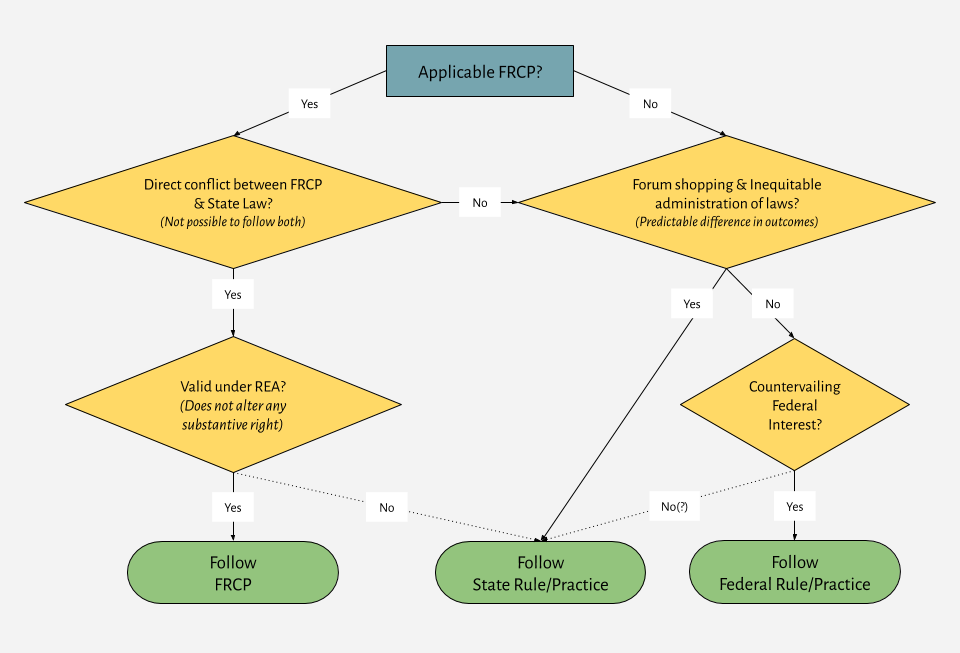
\includegraphics[width=0.9\linewidth,height=\textheight,keepaspectratio]{../img/Erie-Hanna.png}

}

\caption{Erie-Hanna Analysis}

\end{figure}%

\section{Review Questions}\label{review-questions-3}

\subsubsection{Question 1}\label{question-1-2}

Peggy was employed by Sterling Cooper, P.C. She had a written employment
contract specifying a three year term of employment, during which
Sterling Cooper could not terminate Peggy's employment except for cause.
The contract specifies that ``cause for termination includes, but is not
limited to, employee misconduct, dishonesty, or unsatisfactory
performance of assigned duties.''

Before the contract term ended, Peggy was fired. Her boss, Don, told her
the reason was poor performance, but Peggy believes the real reason was
her rejection of Don's repeated and unwelcome advances.

Peggy sues Sterling Cooper in federal court, asserting a claim for
breach of contract under Hudson state law. Assume the court has personal
and subject matter jurisdiction.

In her complaint, Peggy seeks compensatory damages for her loss of
employment.

\paragraph{Part A}\label{part-a-1}

Under Hudson state law, compensatory damages for wrongful termination in
breach of an employment contract are limited to an amount equal to three
times the plaintiff's annual earnings (wages or salary) in their last
year of employment. In contrast, in cases for wrongful termination under
federal law, there is no such cap on the amount of compensatory damages.

\emph{Which rule should the federal court apply in this case?}

\paragraph{Part B}\label{part-b-1}

Under Hudson state law, a complaint for breach of contract must include
an itemized statement showing the basis and amount of compensatory
damages sought. In contract, under FRCP Rule 8(a)(3), the ``demand for
relief sought'' requires only a general statement that the plaintiff
seeks compensatory damages.

\emph{Which rule should the federal court apply in this case?}

\subsubsection{Question 2}\label{question-2-2}

The Carbolic Smoke Ball Company (``Carbolic'') runs an ad in the Pall
Mall Gazette. The ad claims that the company's Carbolic Smoke Ball is
``clinically proven to prevent colds and flu when used as directed.'' In
fact, the product does nothing at all, other than emit foul-smelling
smoke, and the company never conducted any tests, clinical or otherwise.

After reading the ad, Carlill buys a Carbolic Smoke Ball and uses it as
directed three times a day for several weeks. She is chagrined when she
contracts the flu anyway. It turns out to be an especially bad case of
the flu, requiring hospitalization and expensive medical treatment.

Carlill sues Carbolic for fraud under Euphoria state law. Her complaint
alleges that Carbolic's ad made false claims about the health benefits
of the Smoke Ball, that Carbolic knew those claims were false, and that
Carbolic made those claims with an intent to induce consumers to buy the
product. In the complaint, Carlill requests the following relief:

\begin{enumerate}
\def\labelenumi{\arabic{enumi}.}
\tightlist
\item
  \$80,000 in punitive and compensatory damages, and
\item
  a permanent injunction prohibiting Carbolic from making false claims
  about the Carbolic Smoke Ball's health benefits.
\end{enumerate}

Carlill files her suit in the U.S. District Court for the District of
Euphoria, which has subject matter jurisdiction based on diversity of
citizenship.

\paragraph{Part A}\label{part-a-2}

FRCP Rule 8(a)(3) provides that a complaint must include ``a demand for
the relief sought, which may include relief in the alternative or
different types of relief.'' Under this rule, a plaintiff may request
both legal remedies (usually money damages) and equitable relief (such
as an injunction) in the same complaint.

In contrast, under Euphoria state law, a plaintiff who seeks both legal
remedies and equitable relief must file two complaints, one seeking the
legal remedy and another seeking the equitable relief. Both complaints
will go to the same court, which will treat them as a single action for
most purposes. If (either on summary judgment or at trial) the defendant
is found liable, the court will then hold a separate hearing to
determine whether the plaintiff is entitled to the injunction or other
equitable relief sought.

Carbolic objects that Carlill's request for both money damages and an
injunction in the same complaint is improper under Euphoria law. Carlill
argues that federal law, not state law, governs whether she may seek
both types of relief in the same complaint.

\emph{Should the court apply state or federal law on this issue?}

\paragraph{Part B}\label{part-b-2}

Under Euphoria state law, a consumer asserting a fraud claim based on an
allegedly false advertisement must plead and prove the following
elements:

\begin{enumerate}
\def\labelenumi{\arabic{enumi}.}
\tightlist
\item
  The defendant made false claims about the product
\item
  The defendant knew the claims were false
\item
  The defendant made the claims with the intent to induce consumers to
  buy the product
\item
  The plaintiff reasonably relied on the claims in deciding to buy the
  product.
\end{enumerate}

In contrast, under the FTC Act (a federal statute), an advertiser is
liable for false advertising even if it was unreasonable for a consumer
to have relied on the defendant's false claims. The FTC Act authorizes
the Federal Trade Commission to bring civil suits for false advertising,
but does not give individual consumers a private right of action.

The Company moves to dismiss Carlill's complaint for failure to state a
claim, because the complaint fails to allege that Carlill reasonably
relied on the claims in the ad regarding the supposed health benefits of
the Carbolic Smoke Ball.

\emph{Should the federal court apply state or federal law on the issue
of whether Carlill must allege and prove reasonable reliance?}

\chapter{Pleading}\label{pleading}

\section{Pleading Under the FRCP}\label{pleading-under-the-frcp}

\subsection{Fed. R. Civ. P. Rule 3}\label{fed.-r.-civ.-p.-rule-3}

A civil action is commenced by filing a complaint with the court.

\subsection{Fed. R. Civ. P. Rule 7}\label{fed.-r.-civ.-p.-rule-7}

(a) Pleadings. Only these pleadings are allowed:

\begin{itemize}
\item
  (1) a complaint;
\item
  (2) an answer to a complaint;
\item
  (3) an answer to a counterclaim designated as a counterclaim;
\item
  (4) an answer to a crossclaim;
\item
  (5) a third-party complaint;
\item
  (6) an answer to a third-party complaint; and
\item
  (7) if the court orders one, a reply to an answer.
\end{itemize}

(b) Motions and Other Papers.

\begin{itemize}
\item
  (1) In General. A request for a court order must be made by motion.
  The motion must:

  \begin{itemize}
  \item
    (A) be in writing unless made during a hearing or trial;
  \item
    (B) state with particularity the grounds for seeking the order; and
  \item
    (C) state the relief sought.
  \end{itemize}
\item
  (2) Form. The rules governing captions and other matters of form in
  pleadings apply to motions and other papers.
\end{itemize}

\subsection{Fed. R. Civ. P. Rule 8}\label{fed.-r.-civ.-p.-rule-8}

(d) Pleading to Be Concise and Direct; Alternative Statements;
Inconsistency.

\begin{itemize}
\item
  (1) \emph{In General.} Each allegation must be simple, concise, and
  direct. No technical form is required.
\item
  (2) \emph{Alternative Statements of a Claim or Defense.} A party may
  set out 2 or more statements of a claim or defense alternatively or
  hypothetically, either in a single count or defense or in separate
  ones. If a party makes alternative statements, the pleading is
  sufficient if any one of them is sufficient.
\item
  (3) \emph{Inconsistent Claims or Defenses.} A party may state as many
  separate claims or defenses as it has, regardless of consistency.
\end{itemize}

(e) Construing Pleadings. Pleadings must be construed so as to do
justice.

\subsection{Fed. R. Civ. P. Rule 10}\label{fed.-r.-civ.-p.-rule-10}

(a) Caption; Names of Parties. Every pleading must have a caption with
the court's name, a title, a file number, and a Rule 7(a) designation.
The title of the complaint must name all the parties; the title of other
pleadings, after naming the first party on each side, may refer
generally to other parties.

(b) Paragraphs; Separate Statements. A party must state its claims or
defenses in numbered paragraphs, each limited as far as practicable to a
single set of circumstances. A later pleading may refer by number to a
paragraph in an earlier pleading. If doing so would promote clarity,
each claim founded on a separate transaction or occurrence---and each
defense other than a denial---must be stated in a separate count or
defense.

(c) Adoption by Reference; Exhibits. A statement in a pleading may be
adopted by reference elsewhere in the same pleading or in any other
pleading or motion. A copy of a written instrument that is an exhibit to
a pleading is a part of the pleading for all purposes.

\subsection{Fed. R. Civ. P. Rule 12}\label{fed.-r.-civ.-p.-rule-12}

(e) Motion for a More Definite Statement. A party may move for a more
definite statement of a pleading to which a responsive pleading is
allowed but which is so vague or ambiguous that the party cannot
reasonably prepare a response. The motion must be made before filing a
responsive pleading and must point out the defects complained of and the
details desired. If the court orders a more definite statement and the
order is not obeyed within 14 days after notice of the order or within
the time the court sets, the court may strike the pleading or issue any
other appropriate order.

(f) Motion to Strike. The court may strike from a pleading an
insufficient defense or any redundant, immaterial, impertinent, or
scandalous matter. The court may act:

\begin{itemize}
\item
  (1) on its own; or
\item
  (2) on motion made by a party either before responding to the pleading
  or, if a response is not allowed, within 21 days after being served
  with the pleading.
\end{itemize}

\subsection{Doe v. Clinton County (W.D. Mich.
2025)}\label{doe-v.-clinton-county-w.d.-mich.-2025}

\subsubsection{Order Striking Complaint}\label{order-striking-complaint}

Each page {\marginnote{\begin{footnotesize}The first page of the
complaint is reproduced below. Surprisingly, the court did not mention
the egregious use of colored type in the complaint. Many federal and
state courts have local rules governing the typography of pleadings,
motions, briefs, and other documents. Butterick (2015) is a very useful
guide to producing attractive, reader-friendly, legal
documents.\end{footnotesize}}} of plaintiff's complaint appears on an
e-filing which is dominated by a large multi-colored cartoon dragon
dressed in a suit, presumably because she is represented by the law firm
of ``Dragon Lawyers PC © Award Winning Lawyers''. Fed. R. Civ. P.
12(f)(1) allows a court to ``strike from a pleading \ldots{} any
redundant, immaterial, impertinent, or scandalous matter.'' Use of this
dragon cartoon logo is not only distracting, it is juvenile and
impertinent. The Court is not a cartoon. Accordingly,

\textbf{IT IS ORDERED} that plaintiff's complaint is \textbf{STRICKEN}.
Plaintiff is directed to file an amended complaint, containing the same
allegations as the original complaint, without the cartoon dragon by no
later than May 5, 2025.

\textbf{IT IS FURTHER ORDERED} that plaintiff shall not file any other
documents with the cartoon dragon or other inappropriate content.

\begin{figure}[H]

{\centering 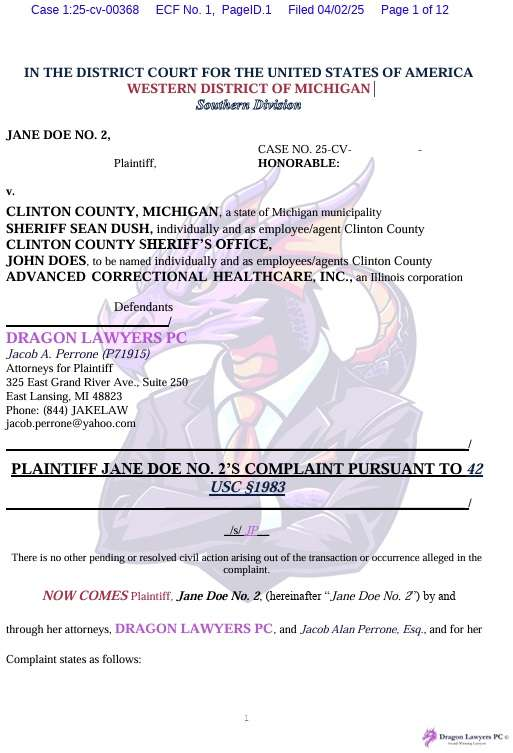
\includegraphics[width=0.5\linewidth,height=\textheight,keepaspectratio]{../img/DragonComplaint.jpg}

}

\caption{Doe v. Clinton County Complaint}

\end{figure}%

\subsection{Smith v. Safemarine Corp.~(M.D.~Louisiana
2024)}\label{smith-v.-safemarine-corp.-m.d.-louisiana-2024}

{[}\textbf{Summary of the Facts.} \emph{Plaintiff sued multiple
defendants---including Archer Daniels Midland Company (``ADM''), ARTCO
Stevedoring (``ARTCO''), Riverside Shipping (``Riverside''), and Phoenix
Bulk Carriers (``Phoenix Bulk'')---in connection with injuries he
sustained while working aboard a container ship called the M/V Eva
Paris. Defendants filed motions for a more definite statement under Rule
12(e), contending that the complaint contained insufficient factual
detail regarding each defendants' role in the accident and the basis for
liability.}{]}

The United States Supreme Court {[}has{]} set forth the basic criteria
necessary for a complaint to survive a Rule 12(b)(6) motion to dismiss:
``While a complaint attacked by a Rule 12(b)(6) motion to dismiss does
not need detailed factual allegations, a plaintiff's obligation to
provide the grounds of his entitlement to relief requires more than
labels and conclusions, and a formulaic recitation of the elements of a
cause of action will not do.''{\marginnote{\begin{footnotesize}See §6.3
Claims for Relief.\end{footnotesize}}} A complaint is also insufficient
if it merely ``tenders `naked assertions' devoid of `further factual
enhancement.'\,'' However, ``a claim has facial plausibility when the
plaintiff pleads the factual content that allows the court to draw the
reasonable inference that the defendant is liable for the misconduct
alleged.'' In order to satisfy the plausibility standard, the plaintiff
must show ``more than a sheer possibility that a defendant has acted
unlawfully.'' ``Furthermore, while the court must accept well-pleaded
facts as true, it will not `strain to find inferences favorable to the
plaintiff.'\,'' On a motion to dismiss, courts ``are not bound to accept
as true a legal conclusion couched as a factual allegation.''

Rule 12(e) provides that a motion for more definite statement may be
filed when ``a pleading to which a responsive pleading is permitted is
so vague or ambiguous that a party cannot reasonably be required to
frame a responsive pleading.'' The standard for evaluating a motion for
more definite statement is whether the complaint ``is so excessively
vague and ambiguous as to be unintelligible and as to prejudice the
defendant seriously in attempting to answer it.'' Such motions are
disfavored and granted sparingly. However, in the words of the Supreme
Court, ``if a pleading fails to specify the allegations in a manner that
provides sufficient notice,'' then a Rule 12(e) motion may be
appropriate. A party may not use a Rule 12(e) motion as a substitute for
discovery; however, ``if details are necessary in order to make a vague
complaint intelligible, the fact that the details also are subject to
the discovery process should not preclude their production under Rule
12(e).''

As other courts have noted, ``the line between Rule 12(b)(6) and Rule
12(e)'s pleading standards is a blurry one.'' Regarding the relationship
between the two, it has been observed that ``an implausible claim may
well be stated intelligibly enough to enable the framing of a response,
and a plausible claim, which would survive a Rule 12(b)(6) motion, may
be pleaded vaguely enough to make response impossible, which would make
it vulnerable to a Rule 12(e) motion.''

In separate paragraphs, Plaintiff's Petition for Damages
{\marginnote{\begin{footnotesize}The plaintiff originally filed his suit
in Louisiana state court, where ``Petition for Damages'' is the term
used for a civil complaint. The case was removed to federal court based
on diversity of citizenship.\end{footnotesize}}} identifies and
introduces each Defendant by name and corporate status, as well as their
addresses and agents for service of process. Apart from the singular
introductory paragraphs, there is no additional information in the
Petition regarding ARTCO or ADM. As to the other moving Defendants,
Plaintiff additionally alleges that Riverside and Phoenix Bulk, ``either
individually, collectively, or in combination \ldots{} owned, operated,
assumed contractual responsibility, or otherwise exercised significant
control over the M/V EVA PARIS and/or its shipment of bulk concrete, to
which Plaintiff was assigned and aboard which Plaintiff was injured.''

The Petition goes on to provide that Plaintiff ``lost his balance after
stepping in a pile of concrete that had been spilled during unlading of
the Vessel's cargo and not properly cleaned,'' as a result of which
Plaintiff ``fell multiple feet from the deck of the ship into the
Mississippi River, and nearly drowned but-for a coworker pulling him out
of the water.'' Plaintiff then provides a list of eighteen theories of
liability without explaining which Defendant may be liable for which
theory, and on what grounds. Similarly, Plaintiff alleges that
``Defendants owed Plaintiff a duty consistent with the foregoing, and
Defendants' various acts and omissions which proximately caused
Plaintiff to encounter the hazardous condition aboard the Vessel
consisted of a breach of said duties.'' Plaintiff does not provide any
detail regarding these ``various acts or omissions'' allegedly committed
by the Defendants or what duties each Defendant breached as a result.

The Court finds that it is entirely unclear from a reading of the
Petition what role each Defendant allegedly played in the incident or
how each may be liable to Plaintiff. The Petition does not outline the
connection between the few factual allegations and the legal theories
and fails to specify which theories apply to which Defendants.

``If the pleading is impermissibly vague, the court may act under Rule
12(b)(6) or Rule 12(e), whichever is appropriate, without regard to how
the motion is denominated.'' Under the present circumstances, the Court
finds Defendants' motions for a more definite statement meritorious
under Rule 12(e) because the primary grievance of all the moving
Defendants is that the Petition is simply too vague.

The Supreme Court has stated that Rule 12(e) motions are ``inextricably
linked to Rule 8(a)'s simplified notice pleading standard.''
Accordingly, ``when evaluating a motion for more definite statement, the
Court must assess the complaint in light of the minimal pleading
requirements of Rule 8.'' Rule 8 provides, in pertinent part: ``A
pleading that states a claim for relief must contain \ldots{} a short
and plain statement of the claim showing that the pleader is entitled to
relief.'' The allegations must ``give the defendant fair notice of what
the plaintiff's claim is and the grounds upon which it rests.'' This
pleading standard ``does not require `detailed factual allegations,' but
it demands more than an unadorned, the-defendant-unlawfully-harmed-me
accusation.''

Here, the Petition lacks any factual allegations regarding the subject
incident other than a brief description of Plaintiff's fall and
injuries. As to ADM and ARTCO, the Petition contains no information
whatsoever regarding their roles in or relationship to the incident. As
to Phoenix Bulk and Riverside, Plaintiff broadly alleges that they,
``either individually, collectively, or in combination \ldots{} owned,
operated, assumed contractual responsibility, or otherwise exercised
significant control over'' the Vessel or its shipment of concrete. Other
than a bare list of generic theories of liability and conclusory
statements, such as ``Defendants acted with flagrant and malicious
disregard of Plaintiff's health and safety,'' the Petition does not
convey with adequate specificity or clarity how the Defendants are
responsible for Plaintiff's alleged injuries. As Phoenix Bulk argues,
``because Plaintiff has failed to actually allege any specific facts
with respect to Phoenix Bulk, Phoenix Bulk cannot discern exactly what
claim Plaintiff files against it or why Phoenix Bulk should be liable in
the first instance.'' The same is true for each moving Defendant.

The Court finds that Plaintiff's Petition lacks sufficient specificity
to give the moving Defendants adequate notice of grounds upon which the
claims are premised. Accordingly, because the Petition is ``so vague or
ambiguous that the Defendants cannot reasonably prepare a response,''
the Court finds the Rule 12(e) motion of each Defendant should be
granted.

\section{Claims for Relief}\label{claims-for-relief}

\subsection{Fed. R. Civ. P. Rule 8}\label{fed.-r.-civ.-p.-rule-8-1}

(a) Claim for Relief. A pleading that states a claim for relief must
contain:

\begin{itemize}
\item
  (1) a short and plain statement of the grounds for the court's
  jurisdiction, unless the court already has jurisdiction and the claim
  needs no new jurisdictional support;
\item
  (2) a short and plain statement of the claim showing that the pleader
  is entitled to relief; and
\item
  (3) a demand for the relief sought, which may include relief in the
  alternative or different types of relief.
\end{itemize}

\subsection{Fed. R. Civ. P. Rule 9}\label{fed.-r.-civ.-p.-rule-9}

(a) Capacity or Authority to Sue; Legal Existence.

\begin{itemize}
\item
  (1) \emph{In General.} Except when required to show that the court has
  jurisdiction, a pleading need not allege:

  \begin{itemize}
  \item
    (A) a party's capacity to sue or be sued;
  \item
    (B) a party's authority to sue or be sued in a representative
    capacity; or
  \item
    (C) the legal existence of an organized association of persons that
    is made a party.
  \end{itemize}
\item
  (2) \emph{Raising Those Issues.} To raise any of those issues, a party
  must do so by a specific denial, which must state any supporting facts
  that are peculiarly within the party's knowledge.
\end{itemize}

(b) Fraud or Mistake; Conditions of Mind. In alleging fraud or mistake,
a party must state with particularity the circumstances constituting
fraud or mistake. Malice, intent, knowledge, and other conditions of a
person's mind may be alleged generally.

(c) Conditions Precedent. In pleading conditions precedent, it suffices
to allege generally that all conditions precedent have occurred or been
performed. But when denying that a condition precedent has occurred or
been performed, a party must do so with particularity.

(f) Time and Place. An allegation of time or place is material when
testing the sufficiency of a pleading.

(g) Special Damages. If an item of special damage is claimed, it must be
specifically stated.

\subsection{Assessing the Sufficiency of a
Claim}\label{assessing-the-sufficiency-of-a-claim}

Under Rule 8(a), a ``pleading that states a claim for relief must
contain {[}\ldots{]} a short and plain statement of the claim showing
that the pleader is entitled to relief''. This requirement applies to
any party (whether in the position of plaintiff or defendant)\footnote{The
  rules governing counterclaims, crossclaims, and third-party claims are
  covered in Chapter 2 (Joinder).} who asserts a claim, counterclaim,
crossclaim, or third-party claim.

A defending party may challenge the sufficiency of a claim under Rule
8(a)(2) with a motion to dismiss for ``failure to state a claim upon
which relief can be granted''. Fed. R. Civ. P. Rule 12(b)(6).\footnote{See
  §4 Responsive Pleadings.} A claim may be dismissed on this basis for
either factual or legal insufficiency:

\begin{itemize}
\item
  • A claim is \emph{factually insufficient} if the facts alleged, even
  assuming they are true, would not satisfy the elements of a claim. For
  example, if a plaintiff asserts a claim for negligence, but fails to
  allege any injury resulting from the defendant's conduct, the claim
  would be factually insufficient, because injury is a necessary element
  of the claim.
\item
  • A claim is \emph{legally insufficient} if the law does not recognize
  the purported claim at all. For example, if a plaintiff sues for
  ``tortious bad taste in music'', alleging that the defendant
  incessantly played ``We Built this City'' by The Starship and
  ``Rockstar'' by Nickleback, the claim would be legally insufficient,
  because the law (regrettably) doesn't recognize any such claim.
\end{itemize}

In \emph{Conley v. Gibson}, 355 U.S. 41 (1957), the Supreme Court
interpreted Rule 8(a)(2) to establish a ``notice pleading'' pleading
standard, requiring only that the plaintiff ``give the defendant fair
notice of what the claim is and the grounds upon which it rests,''
without the necessity for detailed factual allegations. This standard
rested on the structure of the Federal Rules of Civil Procedure, under
which the assertion of claims and the disclosure of facts are allocated
to separate phases of a suit. At the pleading stage, ``a complaint
should not be dismissed for failure to state a claim unless it appears
beyond doubt that the plaintiff can prove no set of facts in support of
his claim which would entitle him to relief.'' The discovery rules then
give the parties an opportunity to establish the facts in full.

A half-century later, a pair of Supreme Court decisions jettisoned the
\emph{Conley} ``no set of facts'' standard and adopted a more demanding
approach.

\subsubsection{Bell Atlantic Corp.~v. Twombly, 550 U.S. 544
(2007)}\label{bell-atlantic-corp.-v.-twombly-550-u.s.-544-2007}

In \emph{Twombly}, the plaintiffs alleged that four telecommunications
companies had ``engaged in a contract, combination or conspiracy to
prevent competitive entry in their respective local telephone and/or
high speed internet services markets by, among other things, agreeing
not to compete with one another and to stifle attempts by others to
compete with them and otherwise allocating customers and markets to one
another in violation of Section 1 of the Sherman Antitrust Act,
\href{https://www.law.cornell.edu/uscode/text/15/1}{15 U.S.C. §1}'' In
support of that claim, the complaint{\marginnote{\begin{footnotesize}You
can read the complaint
\href{../exhibits/Twombly-complaint.pdf}{here}.\end{footnotesize}}}
alleged that the defendants ``engaged in parallel conduct'' to restrict
competition, including ``making unfair agreements with {[}competing
providers{]} for access to {[}the defendants'{]} networks, providing
inferior connections to the networks, overcharging, and billing in ways
designed to sabotage the {[}competing providers'{]} relations with their
own customers.'' The complaint also alleged that the defendants agreed
to refrain from competing with one another, by not pursuing business
opportunities in markets already serviced by other defendants.

\begin{quote}
In the absence of any meaningful competition between {[}the
defendants{]} in one another's markets, and in light of the parallel
course of conduct that each engaged in to prevent competition from
{[}other providers{]} within their respective local telephone and/or
high speed internet services markets and the other facts and market
circumstances alleged above, Plaintiffs allege upon information and
belief that Defendants have entered into a contract, combination or
conspiracy to prevent competitive entry in their respective local
telephone and/or high speed internet services markets and have agreed
not to compete with one another and otherwise allocated customers and
markets to one another.
\end{quote}

The Court held that the allegations in the complaint were insufficient
to state a claim under §1 of the Sherman Act, which requires proof of a
``contract, combination, or conspiracy, in restraint of trade or
commerce''.

\begin{quote}
A plaintiff's obligation to provide the ``grounds'' of his ``entitlement
to relief'' requires more than labels and conclusions, and a formulaic
recitation of the elements of a cause of action will not do. Factual
allegations must be enough to raise a right to relief above the
speculative level, on the assumption that all the allegations in the
complaint are true (even if doubtful in fact).

An allegation of parallel conduct and a bare assertion of conspiracy
will not suffice {[}to state a claim under Sherman Act §1{]}. Without
more, parallel conduct does not suggest conspiracy, and a conclusory
allegation of agreement at some unidentified point does not supply facts
adequate to show illegality. Hence, when allegations of parallel conduct
are set out in order to make a §1 claim, they must be placed in a
context that raises a suggestion of a preceding agreement, not merely
parallel conduct that could just as well be independent action.''
\end{quote}

To assess whether the inference of an agreement was plausible, the
majority considered ``an obvious alternative explanation'': While the
alleged parallel conduct was ``consistent with conspiracy,'' it was, in
the majority's view, ``as much in line with a wide swath of rational and
competitive business strategy unilaterally prompted by common
perceptions of the market.'' Finding that ``the plaintiffs here have not
nudged their claims across the line from conceivable to plausible,'' the
majority concluded that ``their complaint must be dismissed.''

\subsubsection{Ashcroft v. Iqbal, 556 U.S. 662
(2009)}\label{ashcroft-v.-iqbal-556-u.s.-662-2009}

Javaid Iqbal sued various federal government officials, including former
Attorney General John Ashcroft and FBI Director Robert Mueller, over his
arrest and detention as a ``a person `of high interest' to the September
11 investigation''. Iqbal, a citizen of Pakistan and a Muslim, alleged
that Ashcroft and Mueller ``adopted an unconstitutional policy that
subjected him to harsh conditions of confinement on account of his race,
religion, or national origin.''

\begin{quote}
The complaint contends that petitioners designated respondent a person
of high interest on account of his race, religion, or national origin,
in contravention of the First and Fifth Amendments to the Constitution.
The complaint alleges that ``the FBI, under the direction of Defendant
MUELLER, arrested and detained thousands of Arab Muslim men as part of
its investigation of the events of September 11.'' It further alleges
that ``the policy of holding post-September-11th detainees in highly
restrictive conditions of confinement until they were `cleared' by the
FBI was approved by Defendants ASHCROFT and MUELLER in discussions in
the weeks after September 11, 2001.'' Lastly, the complaint posits that
petitioners ``each knew of, condoned, and willfully and maliciously
agreed to subject'' respondent to harsh conditions of confinement ``as a
matter of policy, solely on account of his religion, race, and/or
national origin and for no legitimate penological interest.'' The
pleading names Ashcroft as the ``principal architect'' of the policy,
and identifies Mueller as ``instrumental in its adoption, promulgation,
and implementation,''
\end{quote}

Iqbal's claims were based on \emph{Bivens v. Six Unknown Fed. Narcotics
Agents}, 403 U.S. 388 (1971):

\begin{quote}
In \emph{Bivens}---proceeding on the theory that a right suggests a
remedy---this Court ``recognized for the first time an implied private
action for damages against federal officers alleged to have violated a
citizen's constitutional rights.''
\end{quote}

\begin{quote}
In the limited settings where \emph{Bivens} does apply, the implied
cause of action is the ``federal analog to suits brought against state
officials under 42 U.S.C. §1983.'' Based on the rules our precedents
establish, respondent correctly concedes that Government officials may
not be held liable for the unconstitutional conduct of their
subordinates under a theory of respondeat superior. Because vicarious
liability is inapplicable to \emph{Bivens} and §1983 suits, a plaintiff
must plead that each Government official defendant, through the
official's own individual actions, has violated the Constitution.
\end{quote}

\begin{quote}
The factors necessary to establish a \emph{Bivens} violation will vary
with the constitutional provision at issue. Where the claim is invidious
discrimination in contravention of the First and Fifth Amendments, our
decisions make clear that the plaintiff must plead and prove that the
defendant acted with discriminatory purpose. To state a claim based on a
violation of a clearly established right, respondent must plead
sufficient factual matter to show that petitioners adopted and
implemented the detention policies at issue not for a neutral,
investigative reason but for the purpose of discriminating on account of
race, religion, or national origin.
\end{quote}

The Court reiterated the standard adopted in \emph{Twombly}:

\begin{quote}
Rule 8 does not require ``detailed factual allegations,'' but it demands
more than an unadorned, the-defendant-unlawfully-harmed-me accusation. A
pleading that offers ``labels and conclusions'' or ``a formulaic
recitation of the elements of a cause of action will not do.'' Nor does
a complaint suffice if it tenders ``naked assertions'' devoid of
``further factual enhancement.''
\end{quote}

\begin{quote}
To survive a motion to dismiss, a complaint must contain sufficient
factual matter, accepted as true, to ``state a claim to relief that is
plausible on its face.'' A claim has facial plausibility when the
plaintiff pleads factual content that allows the court to draw the
reasonable inference that the defendant is liable for the misconduct
alleged. The plausibility standard is not akin to a ``probability
requirement,'' but it asks for more than a sheer possibility that a
defendant has acted unlawfully. Where a complaint pleads facts that are
``merely consistent with'' a defendant's liability, it ``stops short of
the line between possibility and plausibility of `entitlement to
relief.'\,''
\end{quote}

\begin{quote}
Two working principles underlie our decision in \emph{Twombly}. First,
the tenet that a court must accept as true all of the allegations
contained in a complaint is inapplicable to legal conclusions.
Threadbare recitals of the elements of a cause of action, supported by
mere conclusory statements, do not suffice. Rule 8 marks a notable and
generous departure from the hypertechnical, code-pleading regime of a
prior era, but it does not unlock the doors of discovery for a plaintiff
armed with nothing more than conclusions. Second, only a complaint that
states a plausible claim for relief survives a motion to dismiss.
Determining whether a complaint states a plausible claim for relief
will, as the Court of Appeals observed, be a context-specific task that
requires the reviewing court to draw on its judicial experience and
common sense. But where the well-pleaded facts do not permit the court
to infer more than the mere possibility of misconduct, the complaint has
alleged---but it has not ``shown''---``that the pleader is entitled to
relief.'' Fed. Rule Civ. Proc. 8(a)(2).
\end{quote}

\begin{quote}
In keeping with these principles a court considering a motion to dismiss
can choose to begin by identifying pleadings that, because they are no
more than conclusions, are not entitled to the assumption of truth.
While legal conclusions can provide the framework of a complaint, they
must be supported by factual allegations. When there are well-pleaded
factual allegations, a court should assume their veracity and then
determine whether they plausibly give rise to an entitlement to relief.
\end{quote}

Applying that standard to Iqbal's complaint, the majority concluded that
the allegations were insufficient to state \emph{Bivins} claims against
Ashcroft and Mueller.

\begin{quote}
We begin our analysis by identifying ``the allegations in the complaint
that are not entitled to the assumption of truth. Respondent pleads that
petitioners''knew of, condoned, and willfully and maliciously agreed to
subject him'' to harsh conditions of confinement ``as a matter of
policy, solely on account of his religion, race, and/or national origin
and for no legitimate penological interest.'' The complaint alleges that
Ashcroft was the ``principal architect'' of this invidious policy, and
that Mueller was ``instrumental'' in adopting and executing it. These
bare assertions, much like the pleading of conspiracy in \emph{Twombly},
amount to nothing more than a ``formulaic recitation of the elements''
of a constitutional discrimination claim, namely, that petitioners
adopted a policy ``\,`because of,' not merely `in spite of,' its adverse
effects upon an identifiable group,'' As such, the allegations are
conclusory and not entitled to be assumed true. To be clear, we do not
reject these bald allegations on the ground that they are unrealistic or
nonsensical. We do not so characterize them any more than the Court in
\emph{Twombly} rejected the plaintiffs' express allegation of a
``\,`contract, combination or conspiracy to prevent competitive
entry,'\,'' because it thought that claim too chimerical to be
maintained. It is the conclusory nature of respondent's allegations,
rather than their extravagantly fanciful nature, that disentitles them
to the presumption of truth.
\end{quote}

\begin{quote}
We next consider the factual allegations in respondent's complaint to
determine if they plausibly suggest an entitlement to relief. The
complaint alleges that ``the FBI, under the direction of Defendant
MUELLER, arrested and detained thousands of Arab Muslim men as part of
its investigation of the events of September 11.'' It further claims
that ``the policy of holding post-September-11th detainees in highly
restrictive conditions of confinement until they were `cleared' by the
FBI was approved by Defendants ASHCROFT and MUELLER in discussions in
the weeks after September 11, 2001.'' Taken as true, these allegations
are consistent with petitioners' purposefully designating detainees ``of
high interest'' because of their race, religion, or national origin. But
given more likely explanations, they do not plausibly establish this
purpose.
\end{quote}

\begin{quote}
The September 11 attacks were perpetrated by 19 Arab Muslim hijackers
who counted themselves members in good standing of al Qaeda, an Islamic
fundamentalist group. Al Qaeda was headed by another Arab Muslim---Osama
bin Laden---and composed in large part of his Arab Muslim disciples. It
should come as no surprise that a legitimate policy directing law
enforcement to arrest and detain individuals because of their suspected
link to the attacks would produce a disparate, incidental impact on Arab
Muslims, even though the purpose of the policy was to target neither
Arabs nor Muslims. On the facts respondent alleges the arrests Mueller
oversaw were likely lawful and justified by his nondiscriminatory intent
to detain aliens who were illegally present in the United States and who
had potential connections to those who committed terrorist acts. As
between that ``obvious alternative explanation'' for the arrests, and
the purposeful, invidious discrimination respondent asks us to infer,
discrimination is not a plausible conclusion.
\end{quote}

\begin{quote}
But even if the complaint's well-pleaded facts give rise to a plausible
inference that respondent's arrest was the result of unconstitutional
discrimination, that inference alone would not entitle respondent to
relief. It is important to recall that respondent's complaint challenges
neither the constitutionality of his arrest nor his initial detention.
Respondent's constitutional claims against petitioners rest solely on
their ostensible ``policy of holding post-September-11th detainees'' in
the {[}maximum security special housing unit{]} once they were
categorized as ``of high interest.'' To prevail on that theory, the
complaint must contain facts plausibly showing that petitioners
purposefully adopted a policy of classifying post-September-11 detainees
as ``of high interest'' because of their race, religion, or national
origin.
\end{quote}

\begin{quote}
This the complaint fails to do. Though respondent alleges that various
other defendants, who are not before us, may have labeled him a person
``of high interest'' for impermissible reasons, his only factual
allegation against petitioners accuses them of adopting a policy
approving ``restrictive conditions of confinement'' for
post-September-11 detainees until they were ``\,`cleared' by the FBI.''
Accepting the truth of that allegation, the complaint does not show, or
even intimate, that petitioners purposefully housed detainees in the
ADMAX SHU due to their race, religion, or national origin. All it
plausibly suggests is that the Nation's top law enforcement officers, in
the aftermath of a devastating terrorist attack, sought to keep
suspected terrorists in the most secure conditions available until the
suspects could be cleared of terrorist activity. Respondent does not
argue, nor can he, that such a motive would violate petitioners'
constitutional obligations. He would need to allege more by way of
factual content to ``nudge'' his claim of purposeful discrimination
``across the line from conceivable to plausible.''
\end{quote}

\subsection{Williams v. Mitchell (4th Circuit
2024)}\label{williams-v.-mitchell-4th-circuit-2024}

This case, now before us after the district court's grant of motions to
dismiss based on the insufficiency of the pleadings, involves a series
of interactions between Plaintiff Brandon Williams and Norfolk,
Virginia, police officers. Officer John D. McClanahan first falsely
charged Williams with misdemeanor trespassing. He then perjured himself
at trial to obtain a conviction. On appeal, Williams exposed
McClanahan's perjury through a recording he had taken of the incident,
and the state appellate court ordered the charge dismissed. Two weeks
later, Norfolk police officers, including McClanahan, responded to an
accident in which Williams had been hit by a speeding drunk driver. They
recognized him immediately as ``the guy that gave McClanahan a ration of
shit.'' The officers allegedly falsified information on the accident
report with the intent of depriving Williams of his property right to
sue the other driver.

Williams brought a claim of retaliation for the exercise of his First
and Sixth Amendment rights against the police officers. He also brought
a conspiracy claim and two Virginia state law claims for intentional
infliction of emotional distress (``IIED''), among others. The district
court granted the officers' motions to dismiss Williams' retaliation
claim, holding that he failed to plead an adverse action, and granted
their motions as to his conspiracy claim upon finding that he failed to
plead a constitutional violation. The court dismissed without prejudice
Williams' state law IIED claims by declining to exercise supplemental
jurisdiction.

Considering the facts as pled, Williams has adequately alleged that the
officers' intentional misrepresentation on the accident report would
likely deter him from recording police activity and defending himself at
trial in the future. Therefore, we reverse the district court's
dismissal of his retaliation claim. Having thus found a plausible
constitutional violation at this stage, we vacate the court's dismissal
of his conspiracy claim and remand the claim for reconsideration
consistent with this opinion. Finally, we vacate the court's dismissal
of Williams' IIED claims, which are also remanded for consideration
consistent with this opinion.

The following facts were alleged in Williams' Second Amended Complaint.
In January 2020, Brandon Williams was detained by Norfolk, Virginia,
police officer John D. McClanahan on a misdemeanor trespassing charge.
Williams recorded his interaction with McClanahan. At trial on the
trespassing charge, McClanahan testified falsely and Williams was
convicted. Williams appealed his conviction and used his recording to
show that McClanahan had lied under oath. The appeals court heard
Williams' argument and dismissed the charges against him on September
15, 2020, recognizing that he never should have been prosecuted.

On September 30, 2020, Williams was seriously injured in a car accident
in Norfolk, Virginia. Williams was operating his vehicle carefully when
he was hit by Rex Aman, who was driving over seventy-five miles per hour
and swerving outside his lane. When various Norfolk police officers
including McClanahan arrived at the scene to investigate the accident,
they pointed at and talked about Williams. Officer Rodney Van Faussien
said, while pointing to Williams, ``this is the guy that gave McClanahan
a ration of shit,'' referring to Williams' defense of his trespassing
charge. Aman's blood alcohol level was .30---well above the legal
limit---and the officers learned of Aman's high speed from eyewitnesses.

Despite information from eyewitnesses, a debris field showing a
high-impact accident, and Aman's blood alcohol level, police officers
falsely stated on the accident report that Aman was driving the speed
limit, had not been drinking, and that his car had suffered a steering
defect. This was allegedly done with the intent to deny Williams his
rights by minimizing the accident and deflecting blame from Aman.

As for his retaliation claim, Williams alleged in the operative
complaint that ``by recording McClanahan during his arrest on the
trespassing charge, and by pointing out that McClanahan had lied during
his testimony on the charge, Williams was exercising his First Amendment
rights.'' He continued that ``by insisting on a trial of the trespassing
charge and by challenging the testimony of McClanahan, Williams was
exercising his Sixth Amendment rights.'' Williams claimed that
Defendants ``intentionally retaliated against him for the exercise of
his rights by misrepresenting facts on the accident report \ldots{}
because they realized that he was the person who `gave McClanahan a
ration of shit,'\,'' and they ``did so with the intent to deprive
Williams of his property right to bring a claim for the injuries from
the accident by trying to minimize the accident and deflect blame from
Aman.'' As a result of Defendants' actions, ``Williams has suffered both
physical and emotional injuries which have included sleep disturbance,
actual physical pain, and a significant exacerbation of post-traumatic
stress disorder.''

Regarding conspiracy, Williams alleged that ``Defendants acted jointly
and in concert for the purposes of denying Williams his constitutional
rights.''

Williams also brought two IIED claims, one related to McClanahan's
perjury, and the second related to the Defendants' conduct at the
accident scene. He alleged that both incidents have caused him physical
and emotional injuries. ims.

We review a district court's dismissal under Rule 12(b)(6) \emph{de
novo} and view the complaint in the light most favorable to the
plaintiff, accepting as true all well-pleaded allegations.

Before us on appeal is the district court's dismissal of Williams'
retaliation, conspiracy, and IIED claims, which will each be addressed
in turn.

\subsubsection{A.}\label{a.}

A plaintiff seeking to recover for First and Sixth Amendment retaliation
must allege that (1) he engaged in protected activity, (2) the defendant
took some action that adversely affected his constitutional rights, and
(3) there was a causal relationship between his protected activity and
the defendant's conduct. We begin by addressing the first and third
elements, which are straightforwardly satisfied.

As for the first element, it is uncontested that Williams engaged in
protected First Amendment activity when he recorded his initial
interaction with McClanahan. ``Creating and disseminating information is
protected speech under the First Amendment,'' including
``{[}r{]}ecording police encounters.'' It is also undisputed that
Williams engaged in protected Sixth Amendment activity by demanding a
trial on the trespassing charge and challenging McClanahan's testimony
at trial. The right to a trial and to confront one's witnesses are
constitutionally protected rights under the Sixth Amendment.

Williams has also adequately pled the third element. For a causal
relationship, a plaintiff must show ``at the very least{[}{]} that the
defendant was aware of plaintiff's engaging in protected activity,'' and
``some degree of temporal proximity.'' Here, Williams has sufficiently
alleged that the Defendants were aware of his First and Sixth Amendment
activity: Van Faussien pointed at Williams and stated to fellow
officers, ``this is the guy that gave McClanahan a ration of shit.'' And
as for temporal proximity, the accident occurred on September 30, 2020,
only fifteen days after the appeals court dismissed the charges against
Williams following his presentation of evidence showing that McClanahan
had lied at trial.

Finally, although the second element requires closer analysis, we also
find that Williams adequately alleged that Defendants' retaliatory
action adversely affected his First and Sixth Amendment rights. To
satisfy this element, a plaintiff must show that a defendant's conduct
resulted in more than a \emph{de minimis} inconvenience to the exercise
of the plaintiff's rights; rather, it must chill the exercise of such
rights such that it would likely deter ``a person of ordinary firmness''
from exercise in the future. While the defendant's conduct must chill
the exercise of a constitutional right, the conduct need not constitute
a constitutional violation in itself. This element requires a ``fact
intensive inquiry that focuses on the status of the speaker, the status
of the retaliator, the relationship between the speaker and the
retaliator, and the nature of the retaliatory acts.'' ``Context
matters,'' as ``the significance of any given act of retaliation will
often depend upon the particular circumstances.

According to Williams, the officers' adverse action was their
intentional misrepresentation of facts on the accident report. In
assessing whether this action would chill the exercise of his First and
Sixth Amendment rights as pled, we consider the relative statuses of
Williams and the officers: Here, there is a significant power imbalance
in Williams' relationship with the police, as he is a Black man who had
recently exposed an officer's perjury. We must also account for the
additional context. The police had previously lied to charge and convict
Williams with misdemeanor trespassing, and then at the accident scene,
the officers allegedly pointed at him, talked about him, and lied again
with the intent of depriving him of his rights, despite his being
severely injured and traumatized in the immediate aftermath of a
high-speed crash. Finally, we must also consider the nature of the
retaliatory acts. The adverse action here is not the mere
misrepresentation of facts on an accident report. It is the officers'
\emph{intentional} misrepresentation---the falsity of the report plus
the animus motivating it.

That the police would purposefully falsify an accident report as payback
for Williams proving his innocence is egregious, and particularly so
where the officers sought to deprive Williams of a potential claim
against a drunk driver where Williams was clearly not at fault. This
demonstrates the extreme lengths these officers were willing to go to
punish Williams for exercising his constitutional rights. These
circumstances would be enough to deter a person of ordinary firmness
from exercising their First and Sixth Amendment rights again in the
future.

Contrary to Defendants' contentions, the fact that Williams was able to
pursue and settle a civil lawsuit against Aman does not doom his
retaliation claim. His claim stems from the officers' misrepresentation
of information in an intentional attempt to interfere with Williams'
rights, which is exactly the kind of government conduct that would chill
someone from exercising their constitutional rights in the future; it
does not matter that such attempted interference may have failed.
Likewise, Williams' success in defending against his trespassing charge
does not counsel a different outcome, as it was this defense that led to
law enforcement's deliberate attempt to deprive him of his property
rights. As Williams' counsel articulated at oral argument, given how the
officers' animus came to bear, ``a reasonable person in that situation
is going to think twice: Do I want to endure that again \ldots{} just to
challenge a simple misdemeanor trespassing charge?'' It is at least
plausible that Williams would be hesitant to record later police
encounters or demand a trial knowing that it could result in
future---and perhaps more grievous---police misrepresentations with the
express purpose of causing him harm.

The accident report's inadmissibility in a civil lawsuit does not change
this analysis. The report is indicative of how police officers would
likely testify at trial, and could also be used to refresh an officer's
recollection or for impeachment purposes. But beyond that, the fact that
the police would eschew their duties and lie with the intent of
depriving Williams of his rights---regardless of whether the officers'
falsification actually impeded any civil lawsuit against Aman--- is
materially adverse.

Viewed in the light most favorable to Williams and at this stage of the
proceedings, law enforcement's intentional misrepresentation would
likely deter a person of ordinary firmness from recording police
activity, challenging an officer's testimony, and vigorously defending
oneself at trial in the future.

Williams has thus alleged a First and Sixth Amendment retaliation claim
sufficient to survive a motion to dismiss, and the district court's
opinion granting Defendants' motions on this claim must be reversed.

\subsubsection{B.}\label{b.}

To state a claim for civil conspiracy under 42 U.S.C. §1983, a plaintiff
must allege that defendants ``acted jointly in concert and that some
overt act was done in furtherance of the conspiracy which resulted in
{[}his{]} deprivation of a constitutional right.''

The district court's analysis on this claim ``began, and ended,'' with
whether Defendants' alleged conduct resulted in a violation of Williams'
constitutional rights. The court only considered potential
constitutional violations under the Fifth and Fourteenth Amendments as
well as a constitutional right to access the courts. But retaliation can
be the constitutional violation for such a conspiracy claim, and counsel
for Defendants Mitchell, Stone, and Van Faussien admitted at oral
argument that reversal on the retaliation claim would necessitate remand
on the conspiracy claim.

Having found that Williams has adequately alleged the deprivation of a
constitutional right---that being his claim of First and Sixth Amendment
retaliation--- Williams' conspiracy claim should be remanded to the
district court for reconsideration.

\subsection{Johnson v. Cricket Council USA, Inc.~(E.D.N.C.
2023)}\label{johnson-v.-cricket-council-usa-inc.-e.d.n.c.-2023}

On April 13, 2021, Johnson and Cricket Council USA, Inc.~entered into a
real property contract (the ``Agreement'') for the purchase and sale of
69.94 acres of land in Fayetteville, North Carolina for \$1,259,460.00.
The Agreement defined the ``Contract Date'' as the date when the
``Agreement had been fully executed by both Buyer and Seller.'' Thus,
the contract date was April 13, 2021. The Agreement defined the
``Examination Period'' as ``the period beginning on the first day after
the Contract Date and extending through 5:00 pm (based upon time at the
locale of the Property) on 90 business days from the contract date.''
The Agreement stated that ``Buyer may extend the Examination Period up
to three 30 day extensions, upon each extension buyer will deposit an
additional \$2,500 non refundable.'' And the Agreement noted that ``TIME
IS OF THE ESSENCE AS TO THE EXAMINATION PERIOD.'' The Agreement defined
the ``Closing Date'' as 30 days after the end of the Examination Period
upon approval from the city. The Agreement did not define ``approval
from the city,'' and the Closing Date section did not include a ``time
is of the essence'' provision.

In October 2021, defendants prepared an Amendment (the ``Amendment'') to
the Agreement, and their agents presented the Agreement to Johnson. When
Johnson received the Amendment, he was not represented by an agent or
attorney. The Amendment redefined the Closing Date to be ``on or before
the day which is Thirty (30) days after Buyer obtains all Governmental
and Municipal Permits including but not limited to Master Site Plan and
Building Construction Plans that are required to build Multifamily Units
including Commercial Development and Sports Fields on the Subject
Land.''

According to Johnson, on November 15, 2021, he executed the Amendment
but the Amendment was dated October 28, 2021. Johnson alleges that the
Amendment is unenforceable for various reasons, including a lack of
consideration, the closing date is so vague and ambiguous as to render
it meaningless, the Agreement is not binding on defendants, and because
defendants failed to properly exercise the three 30-day extensions under
the Agreement.

Defendants respond that Cricket Council USA, Inc.~extended the
examination period three times before seeking to amend the Agreement.
According to defendants, the extensions continued the examination period
until Thursday, November 18, 2021. Moreover, 30 days from the end of
that examination period was Saturday, December 18, 2021, which was then
extended until the next business day, Monday, December 20, 2021.
Defendants also contend that when Cricket Council USA, Inc.~signed the
Amendment, Cricket Council USA, Inc.~paid \$7,500.00 in nonrefundable
extension funds in escrow to Johnson. On January 23, 2023, Johnson
notified defendants that he was terminating the Agreement.

To withstand a Rule 12(b)(6) motion, a pleading ``must contain
sufficient factual matter, accepted as true, to state a claim to relief
that is plausible on its face.'' In considering the motion, the court
must construe the facts and reasonable inferences ``in the light most
favorable to the non-moving party.'' A court need not accept as true a
complaint's legal conclusions, ``unwarranted inferences, unreasonable
conclusions, or arguments.'' Rather, a plaintiff's factual allegations
must ``nudge his claims,'' beyond the realm of ``mere possibility'' into
``plausibility.''

When evaluating a motion to dismiss, a court considers the pleadings and
any materials ``attached or incorporated into the complaint.'' A court
may also consider a document submitted by a moving party if it is
``integral to the complaint and there is no dispute about the document's
authenticity.'' Additionally, a court may take judicial notice of public
records without converting the motion to dismiss into a motion for
summary judgment.

As for Johnson's breach of contract claim against Cricket Council USA,
Inc., Johnson must plausibly allege ``the existence of a contract
between plaintiff and defendant, the specific provisions breached, the
facts constituting the breach, and the amount of damages resulting to
plaintiff from such breach.'' Johnson alleges that Cricket Council USA,
Inc.~breached the Agreement by ``(1) failing to pay the additional
earnest money deposits required to extend the original Examination
Period; (2) failing to close within the time allowed thereby, or within
a commercially reasonable time under the circumstances; and (3) such
other acts and omissions as may be shown at trial.''

As for Johnson's allegations about earnest money deposits, Johnson
plausibly alleges that Cricket Council USA, Inc.~did not properly pay to
extend the examination period of the Agreement. Specifically, Johnson
alleges that the Agreement required Cricket Council USA, Inc.~to pay
Johnson \$2,500 before each 30-day extension of the examination period.
See id. Johnson also alleges that the Agreement required a \$2,500
payment as consideration for the extension and that Cricket Council USA,
Inc.~did not make the necessary \$2,500 payment for any extension of the
examination period. Johnson has plausibly alleged a breach of contract
claim against Cricket Council USA, Inc.

As for Johnson's allegations that Cricket Council USA, Inc.~failed to
close in a reasonable time, absent a ``time is of the essence'' clause,
the parties to a real property purchase agreement are allowed a
``reasonable time after the date set for closing to complete
performance.'' The Amendment states that Cricket Council USA, Inc.~had
30 days to close after obtaining the necessary permits and approvals. On
January 23, 2023, when Johnson purported to terminate the Agreement,
defendants argue that Cricket Council USA, Inc.~had not obtained the
necessary permits. Johnson, however, alleges that he had heard nothing
from defendants about their efforts toward closing, did not know if
Cricket Council USA, Inc.~obtained any permits, and more than a year had
passed between signing the Amendment and terminating the Agreement. The
parties dispute whether defendants told Johnson that Cricket Council
USA, Inc.~would continue to honor the Agreement and whether defendants
would soon close. Johnson has plausibly alleged that Cricket Council
USA, Inc.~failed to close in a reasonable time.

As for Johnson's UDTPA {\marginnote{\begin{footnotesize}The NC Unfair \&
Deceptive Trade Practices Act,
\href{https://www.ncleg.net/EnactedLegislation/Statutes/HTML/ByChapter/Chapter_75.html}{N.C.
Gen.~Stat. §75-1.1}.\end{footnotesize}}} claim against the defendants, a
plaintiff must plausibly allege: (1) an unfair or deceptive act or
practice, (2) in or affecting commerce, and (3) which proximately caused
injury to the plaintiff. ``Whether an act or practice is an unfair or
deceptive practice \ldots{} is a question of law for the court.''

A ``mere breach of contract, even if intentional, is not an unfair or
deceptive act under the UDTPA.'' North Carolina law ``does not permit a
party to transmute a breach of contract claim into a \ldots{} UDTPA
claim \ldots{} because awarding punitive or treble damages would destroy
the parties' bargain.'' If substantial aggravating circumstances
accompany a breach of contract, then those circumstances can create an
UDTPA claim. Generally, such aggravating circumstances include some
element of deception, such as forged documents, lies, or fraudulent
inducements.

Johnson alleges that defendants had superior bargaining power, that
Johnson had no experience with real estate, that defendants caused
Johnson to ``enter into the Amendment in an unfair and deceptive
manner,'' and that defendants disguised their intentions during contract
negotiations. Johnson also alleges upon information and belief that
defendants

\begin{quote}
made false representations to Plaintiff or concealed material facts from
Plaintiff concerning: (1) their true intentions with regard to
Plaintiff's property; (2) their true intentions with regard to whether
they would actually close on the purchase of Plaintiff's property; (3)
their acts and omissions concerning moving forward with obtaining
Government and Municipal Permits and Construction Plans concerning the
Subject Property; (4) their ability to close on the Subject Property;
and, (5) such other acts and omissions as may be shown at trial.
\end{quote}

Johnson's {\marginnote{\begin{footnotesize}The court does not explain
why it regards the allegations as ``conclusory'' nor why they ``do not
plausibly allege a UDTPA claim.'' Can you discern the court's
rationale?\end{footnotesize}}} allegations are conclusory and do not
plausibly allege a UDTPA claim. Thus, the court dismisses Johnson's
UDTPA claim.

As for Johnson's request to pierce the corporate veil, the court must
assess whether Johnson plausibly alleges sufficient facts that would, if
believed, tend to establish the required elements to pierce the
corporate veil under North Carolina's ``instrumentality rule.''
{\marginnote{\begin{footnotesize}``Piercing the corporate veil refers to
a special instance where the court holds the shareholder or director of
a corporation personally liable for the corporation's debts.''
\href{https://www.law.cornell.edu/wex/piercing_the_corporate_veil}{Wex
Legal Dictionary}. In this case, the plaintiff was seeking to hold
Mohammed Qureshi, the CEO and Board Chair of Cricket Council USA,
personally liable for the alleged breach of
contract.\end{footnotesize}}} In order to prevail under the
instrumentality rule, the aggrieved party must establish three elements:
``(1) stockholders' control of the corporation amounts to `complete
domination' with respect to the transaction at issue; (2) stockholders'
use of this control to commit a wrong \ldots; and (3) this wrong or
breach of duty must be the proximate cause of the injury.''

Defendants contend that Johnson fails to plausibly allege these required
elements. Johnson responds that he has sufficiently pled facts for the
court to pierce Cricket Council USA, Inc.'s corporate veil.

In \emph{Fischer}, the North Carolina Court of Appeals cited numerous
factual allegations in the plaintiff's complaint that sufficiently pled
a claim to pierce the corporate veil under the instrumentality rule's
``control'' element. To name a few, the plaintiff {[}in
\emph{Fischer}{]} cited specific asset transfers used to subvert the
corporate form, noted that the owner failed to file annual reports with
the Secretary of State and otherwise comply with corporate formalities,
and alleged that the actions of the owner left the corporation in
question insolvent. The North Carolina Court of Appeals noted that these
allegations addressed three of the four elements of control:
``inadequate capitalization,'' ``noncompliance with corporate
formalities,'' and ``complete domination and control of the corporation
so that it has no independent identity.''

Although the analysis of the control element does not depend on the
presence or absence of any particular factor, Johnson's sole reliance on
the factual allegations that Qureshi is the ``sole or dominant owner of
Cricket Council,'' ``is the President of Cricket Council,'' and
``exercises complete dominion and control over Cricket Council'' does
not suffice. Without more facts indicating ``complete domination, not
only of finances, but of policy and business practices \ldots{} so that
the corporate entity \ldots{} had \ldots{} no separate mind, will or
existence of its own,'' Johnson's allegations are conclusory and do not
plausibly support piercing the corporate veil. Because Johnson's
allegations fail under the first ``control'' element of the
instrumentality rule, the court need not address if the breach of
contract claim is within the ``wrongs'' contemplated by the second
element or address proximate cause. Thus, the court dismisses Johnson's
request to pierce the corporate veil.

\section{Responsive Pleadings}\label{responsive-pleadings}

\subsection{Fed. R. Civ. P. Rule 8}\label{fed.-r.-civ.-p.-rule-8-2}

(b) Defenses; Admissions and Denials.

\begin{itemize}
\item
  (1) In General. In responding to a pleading, a party must:

  \begin{itemize}
  \item
    (A) state in short and plain terms its defenses to each claim
    asserted against it; and
  \item
    (B) admit or deny the allegations asserted against it by an opposing
    party.
  \end{itemize}
\item
  (2) Denials---Responding to the Substance. A denial must fairly
  respond to the substance of the allegation.
\item
  (3) General and Specific Denials. A party that intends in good faith
  to deny all the allegations of a pleading---including the
  jurisdictional grounds---may do so by a general denial. A party that
  does not intend to deny all the allegations must either specifically
  deny designated allegations or generally deny all except those
  specifically admitted.
\item
  (4) Denying Part of an Allegation. A party that intends in good faith
  to deny only part of an allegation must admit the part that is true
  and deny the rest.
\item
  (5) Lacking Knowledge or Information. A party that lacks knowledge or
  information sufficient to form a belief about the truth of an
  allegation must so state, and the statement has the effect of a
  denial.
\item
  (6) Effect of Failing to Deny. An allegation---other than one relating
  to the amount of damages---is admitted if a responsive pleading is
  required and the allegation is not denied. If a responsive pleading is
  not required, an allegation is considered denied or avoided.
\end{itemize}

(c) Affirmative Defenses.

\begin{itemize}
\item
  (1) In General. In responding to a pleading, a party must
  affirmatively state any avoidance or affirmative defense, including:

  \begin{itemize}
  \item
    • accord and satisfaction;
  \item
    • arbitration and award;
  \item
    • assumption of risk;
  \item
    • contributory negligence;
  \item
    • duress;
  \item
    • estoppel;
  \item
    • failure of consideration;
  \item
    • fraud;
  \item
    • illegality;
  \item
    • injury by fellow servant;
  \item
    • laches;
  \item
    • license;
  \item
    • payment;
  \item
    • release;
  \item
    • res judicata;
  \item
    • statute of frauds;
  \item
    • statute of limitations; and
  \item
    • waiver.
  \end{itemize}
\item
  (2) Mistaken Designation. If a party mistakenly designates a defense
  as a counterclaim, or a counterclaim as a defense, the court must, if
  justice requires, treat the pleading as though it were correctly
  designated, and may impose terms for doing so.
\end{itemize}

\subsection{Fed. R. Civ. P. Rule 12}\label{fed.-r.-civ.-p.-rule-12-1}

(a) Time to Serve a Responsive Pleading.

\begin{itemize}
\item
  (1) In General. Unless another time is specified by this rule or a
  federal statute, the time for serving a responsive pleading is as
  follows:

  \begin{itemize}
  \item
    (A) A defendant must serve an answer:

    \begin{itemize}
    \item
      (i) within 21 days after being served with the summons and
      complaint; or
    \item
      (ii) if it has timely waived service under Rule 4(d), within 60
      days after the request for a waiver was sent, or within 90 days
      after it was sent to the defendant outside any judicial district
      of the United States.
    \end{itemize}
  \item
    (B) A party must serve an answer to a counterclaim or crossclaim
    within 21 days after being served with the pleading that states the
    counterclaim or crossclaim.
  \item
    (C) A party must serve a reply to an answer within 21 days after
    being served with an order to reply, unless the order specifies a
    different time.
  \end{itemize}
\item
  (4) Effect of a Motion. Unless the court sets a different time,
  serving a motion under this rule alters these periods as follows:

  \begin{itemize}
  \item
    (A) if the court denies the motion or postpones its disposition
    until trial, the responsive pleading must be served within 14 days
    after notice of the court's action; or
  \item
    (B) if the court grants a motion for a more definite statement, the
    responsive pleading must be served within 14 days after the more
    definite statement is served.
  \end{itemize}
\end{itemize}

(b) How to Present Defenses. Every defense to a claim for relief in any
pleading must be asserted in the responsive pleading if one is required.
But a party may assert the following defenses by motion:

\begin{itemize}
\item
  (1) lack of subject-matter jurisdiction;
\item
  (2) lack of personal jurisdiction;
\item
  (3) improper venue;
\item
  (4) insufficient process;
\item
  (5) insufficient service of process;
\item
  (6) failure to state a claim upon which relief can be granted; and
\item
  (7) failure to join a party under Rule 19.
\item
  A motion asserting any of these defenses must be made before pleading
  if a responsive pleading is allowed. If a pleading sets out a claim
  for relief that does not require a responsive pleading, an opposing
  party may assert at trial any defense to that claim. No defense or
  objection is waived by joining it with one or more other defenses or
  objections in a responsive pleading or in a motion.
\end{itemize}

(g) Joining Motions.

\begin{itemize}
\item
  (1) Right to Join. A motion under this rule may be joined with any
  other motion allowed by this rule.
\item
  (2) Limitation on Further Motions. Except as provided in Rule 12(h)(2)
  or
\item
  (3) a party that makes a motion under this rule must not make another
  motion under this rule raising a defense or objection that was
  available to the party but omitted from its earlier motion.
\end{itemize}

(h) Waiving and Preserving Certain Defenses.

\begin{itemize}
\item
  (1) When Some Are Waived. A party waives any defense listed in Rule
  12(b)(2)--(5) by:

  \begin{itemize}
  \item
    (A) omitting it from a motion in the circumstances described in Rule
    12(g)(2); or
  \item
    (B) failing to either:

    \begin{itemize}
    \item
      (i) make it by motion under this rule; or
    \item
      (ii) include it in a responsive pleading or in an amendment
      allowed by Rule 15(a)(1) as a matter of course.
    \end{itemize}
  \end{itemize}
\item
  (2) When to Raise Others. Failure to state a claim upon which relief
  can be granted, to join a person required by Rule 19(b), or to state a
  legal defense to a claim may be raised:

  \begin{itemize}
  \item
    (A) in any pleading allowed or ordered under Rule 7(a);
  \item
    (B) by a motion under Rule 12(c); or
  \item
    (C) at trial.
  \end{itemize}
\item
  (3) Lack of Subject-Matter Jurisdiction. If the court determines at
  any time that it lacks subject-matter jurisdiction, the court must
  dismiss the action.
\end{itemize}

\subsection{Reis Robotics USA, Inc.~v. Concept Industries (N.D. Ill.
2006)}\label{reis-robotics-usa-inc.-v.-concept-industries-n.d.-ill.-2006}

This is a diversity action governed by Illinois law in which Plaintiff
Reis Robotics USA, Inc.~(``Reis'') filed a complaint against Defendant
Concept Industries, Inc.~(``Concept''), seeking redress for breach of
contract. Concept has answered the complaint, asserted six affirmative
defenses, and brought seven counterclaims against Reis. Reis now moves
to strike and dismiss Concept's affirmative defenses; strike portions of
Concept's answer; and dismiss Concept's counterclaims. For the reasons
set forth below, Reis's motions are granted in part and denied in part.

\subsubsection{Background}\label{background-3}

The following facts are taken from Reis's complaint. Reis, an Illinois
corporation, manufactures and supplies industrial robotics equipment.
Concept, a Michigan corporation, manufactures and supplies automotive
parts. On or about February 24, 2005, the parties entered into a
contractual arrangement for Concept to purchase from Reis a robotic
laser cutting machine (the ``Laser'') and associated fixtures for
trimming three separate automotive parts: the Hush Panel, JS Dash
Silencer, and JS Dash Close Out Panel. The pertinent contract documents
are an ``Order Acknowledgment'' executed by Reis and an ``Amended
Purchase Order'' executed by Concept. For ease of reference, we refer to
these documents collectively as ``the Agreement.''

While Reis was in the process of manufacturing the Laser and fixtures
pursuant to the Agreement, Concept informed Reis that Concept had
terminated the Hush Panel program and that the associated fixtures were
no longer needed. The parties agreed to amend the purchase price of the
Agreement to reflect the cancellation of the Hush Panel fixtures but to
include payment for work performed. Following the cancellation of the
Hush Panel fixtures, the amended purchase price of the Agreement was
\$911,000.

In July 2005, Reis presented and demonstrated the Laser to Concept. In
August 2005, Concept informed Reis of changes to the JS Dash Silencer
part. Concept's changes to the JS Dash Silencer part required Reis to
redesign the associated fixtures. Reis alleges that Concept ordered
these modifications under the Agreement, but Concept denies this
allegation. Reis asserts that it is entitled to the original purchase
price of the JS Dash Silencer fixtures and for work performed on their
redesign and remanufacture.

In October 2005, Reis again presented and demonstrated the Laser to
Concept. On October 3, 2005, Concept acknowledged receipt of the Laser
at its Michigan facility by executing an Acceptance Test Certificate.

In November 2005, Concept informed Reis that Concept had terminated the
JS Dash Close Out Panel program and that the associated fixtures, which
Reis was still working on, were no longer needed. Reis alleges that it
was entitled to payment for work already performed on the JS Dash Close
Out Panel fixtures prior to cancellation, a total of \$6,900. Concept
denies that Reis is entitled to payment of this amount.

The parties agree that Concept has paid' Reis \$588,600 to date. Reis
asserts that Concept has breached the Agreement by failing to pay a
remaining balance of \$264,300 plus interest. Concept denies that it
owes Reis any additional money under the Agreement.

The following additional facts are gleaned from Concept's ``Answer,
Affirmative Defenses and Counterclaim.'' Concept alleges that prior to
entering the Agreement, the parties engaged in extensive negotiations
regarding the specifications of the Laser, particularly the Laser's
cutting speed, also called ``cycle time,'' meaning the time required to
complete one part. Throughout the negotiations, Reis, through its sales
manager Dino Chece, allegedly made various oral and written promises to
Concept indicating that the Laser would trim the JS Dash Silencer parts
at a cycle time of 60-70 seconds per part or faster. Relying on these
promises by Reis, Concept entered into the Agreement.

The Agreement stated that the ``Application'' of the Laser was for the
cutting of parts ``described as Hush Panel/Panels Close/Silencer.'' The
Agreement did not mention the 60-70 seconds cycle time, but did provide
as follows:

\begin{quote}
Necessary cycle time per component is indicated from Concept Industries
with 23.7 sec per part including loading/ unloading and inspection.
During our test in Chicago we were able to cut the parts in 17-20
sec.~The table rotating time is 3 sec.~The loading/unloading as well as
inspection is done during {[}sic{]} the robot is cutting the part,
therefore this time does not need to be added to the overall cycle. Reis
Robotics is NOT responsible for the Operator related cycle times.
\end{quote}

The Agreement also contained an express warranty that the Laser would be
free from defects in material and workmanship.

According to Concept, at a demonstration of the Laser conducted by Reis
on May 26, 2005, Concept personnel questioned Mr.~Chece and Dr.~Wenzel,
Reis's general manager, about the Laser's apparent slow cutting speed of
JS Dash Silencer parts during the demonstration. In response to
Concept's concerns, Mr.~Chece and Dr.~Wenzel responded that the Laser
was not yet optimized and that Concept had ``nothing to worry about.''
When Concept accepted possession of the Laser at its facility, the
certificate of acceptance indicated that cycle times ``cannot be checked
without the production fixture.'' Following the installation of the
Laser at Concept's facility, Concept repeatedly expressed to Reis
concerns regarding the cutting speed of the Laser. Concept repeatedly
requested assurances from Reis that the cycle time for the JS Dash
Silencer would be 60-70 seconds per part, as promised earlier by
Mr.~Chece. After it became clear to Concept that the Laser would be
unable to achieve the promised cycle time, on December 21, 2005, a
representative of. Concept sent Reis an email informing Reis that
``Concept is pursuing the implementation of an alternate production
process'' and requesting that Reis ``place all production fixtures
design work that is currently in-process on the LHD and RHD JS Dash
Silencers on hold.''

On January 6, 2006, Reis informed Concept in writing that the Laser's
cycle time for the JS Dash Silencer would be between 150-195 seconds per
part, far longer than what was originally promised. According to
Concept, to date the Laser has failed to come close to achieving the
initially promised cycle time of 60-70 seconds per part, a defect that
was. ``fatal'' to Concept's ability to manufacture parts in the volumes
required by its customers.

As for the JS Dash Silencer fixtures, Concept alleges that it only
authorized Reis to design the JS Dash Silencer fixtures and never
authorized Reis to begin manufacturing the fixtures. According to
Concept, between April and October 2005, the parties exchanged numerous
communications through which both parties indicated that Reis would wait
for Concept's final design approval prior to initiating any production
of the JS Dash Silencer fixtures. Concept alleges that it never gave
Reis final design approval and therefore is not responsible for any
charges related to the production of the JS Dash Silencer fixtures.

Concept also raises counterclaims against Reis for: (1) fraudulent
inducement; (2) misrepresentation; (3) unjust enrichment; (4) promissory
estoppel; (5) breach of contract; (6) breach of express warranty; and
(7) overpayment. All of the claims are premised on the Laser's inability
to achieve the cycle time allegedly discussed by the parties.

\subsubsection{Motion to Strike and Dismiss Affirmative
Defenses}\label{motion-to-strike-and-dismiss-affirmative-defenses}

We turn first to Reis's motion to strike and dismiss various portions of
Concept's affirmative defenses.

Federal Rule of Civil Procedure 12(f) permits the Court to strike ``any
insufficient defense or any redundant, immaterial, impertinent or
scandalous matter.'' Fed.R.Civ.P. 12(f). Motions to strike are generally
disfavored because of their potential to delay proceedings. Nonetheless,
a motion to strike can be a useful means of removing ``unnecessary
clutter'' from a case, which will in effect expedite the proceedings.

Affirmative defenses are pleadings and, as such, are subject to all the
same pleading requirements applicable to complaints. Thus, affirmative
defenses must set forth a ``short and plain statement'' of the basis for
the defense. Fed. R.Civ.P. 8(a). Even under the liberal notice pleading
standards of the Federal Rules, an affirmative defense must include
either direct or inferential allegations as to all elements of the
defense asserted. ``Bare bones conclusory allegations'' are not
sufficient.

This Court applies a three-part test for examining the sufficiency of an
affirmative defense. First, we determine whether the matter is
appropriately pled as an affirmative defense Second, we determine
whether the defense is adequately pled under Federal Rules of Civil
Procedure 8 and 9. \emph{Id.} Third, we evaluate the sufficiency of the
defense pursuant to a standard identical to Federal Rule of Civil
Procedure 12(b)(6). Before granting a motion to strike an affirmative
defense, the Court must be convinced that there are no unresolved
questions of fact, that any questions of law are clear, and that under
no set of circumstances could the defense succeed. Additionally, in a
case premised on diversity jurisdiction, ``the legal and factual
sufficiency of an affirmative defense is examined with reference to
state law.'' With these principles in mind, we turn to the specific
arguments raised in the motion.

For its first affirmative defense Concept asserts: ``The complaint fails
to state a claim upon which relief can be granted.'' Reis argues that
this is not a proper affirmative defense. There is some debate in this
District regarding whether ``failure to state a claim'' may be raised as
an affirmative defense or instead must be raised by separate motion.
Notably, as one court in this District has observed, although failure to
state a claim, may not meet the technical definition of an affirmative
defense, Form 20 of the Federal Rules of Civil Procedure's Appendix of
Forms lists ``failure to state a claim'' as a model defense. Rule 84
specifically authorizes the use of the model defenses contained in the
Forms. Fed.R.Civ.P. 84. In light of Rule 84 and Form 20, we find
authority under the Federal Rules to permit an affirmative defense based
on failure to state a claim.

Nonetheless, Concept has failed to adequately plead the defense in
accordance with Rule 8. Concept's first affirmative defense is nothing
more than a recitation of the standard for a motion to dismiss under
Rule 12(b)(6). As alleged, the defense provides no explanation as to how
and in what portion of the complaint Reis has failed to state a claim.
Although Concept's counterclaim contains detailed factual allegations,
these allegations are not mentioned or incorporated by reference in the
affirmative defenses. Additionally, it is not clear what portion of the
lengthy counterclaim allegations are intended to support Concept's
failure to state a claim defense. The Court agrees that clarity is
needed as to the basis of this defense, and accordingly, the first
affirmative defense is stricken without prejudice.

As its second affirmative defense Concept states: ``Reis breached the
contract on which it purports to rely, and that contract may be void for
fraud and/or failure of consideration.'' Breach of contract, fraud, and
failure of consideration are all matters that may be pled as affirmative
defenses. \emph{See} Fed.R.Civ.P. 8(c). However, the Court agrees with
Reis that Concept's defenses, as pled, do not satisfy the pleading
requirements of Rule 8(a). The breach of contract defense fails to make
reference to any of the elements of a breach of contract claim, and
additionally, Concept fails to plead with heightened particularity the
alleged circumstances constituting fraud as required by Rule 9(b).
Again, although Concept has included detailed allegations in its
counterclaim, it does not link these allegations in any way to the
affirmative defenses, nor is it clear what particular paragraphs of the
counterclaim allegations would apply to this affirmative defense.
Accordingly, the Court strikes Concept's second affirmative defense
without prejudice.

As its third affirmative defense, Concept alleges: ``Reis's payment
claims for the silencer fixture are barred because Concept never
authorized Reis to begin manufacturing the fixture, as Reis itself has
acknowledged.'' Reis argues that this affirmative defense is legally
inadequate. The concept of an affirmative defense under Rule 8(c)
``requires a responding party to \emph{admit} a complaint's allegations
but then permits the responding party to assert that for some legal
reason it is nonetheless excused from liability (or perhaps from full
liability).'' Concept's third affirmative defense does not meet this
criteria, but instead is merely a restatement of the denials contained
in its answer. As such, the affirmative defense is not only unnecessary
but also improper. However, to the extent Concept intended to raise some
affirmative matter here, the Court will give Concept an opportunity to
replead. Accordingly, the third affirmative defense is stricken without
prejudice.

As its fourth affirmative defense, Concept alleges: ``Reis's claims are
subsumed by Concept's right of set-off and/or recoupment. Alternatively,
the amount of Concept's claims against Reis exceeds the amount of Reis's
claim against Concept.'' Reis argues that the affirmative defense is
nothing more than a recapitulation of Concept's denial of the amount of
damages claimed to be owed in the complaint. In its response brief,
Concept fails to offer any analysis refuting Reis's argument. The Court
agrees that this affirmative defense appears to be simply a restatement
of the denials contained in Concept's answer, which is improper.
However, to the extent Concept intended to raise some affirmative matter
here, the Court will give Concept an opportunity to replead. The fourth
affirmative defense is therefore stricken without prejudice.

Concept's fifth affirmative defense states: ``Reis's claims are barred
or limited by laches, waiver, estoppel, unclean hands, or similar legal
or equitable doctrines.'' Laches, waiver, estoppel, and unclean hands
are equitable defenses that must be pled with the specific elements
required to establish the defense. Merely stringing together a long list
of legal defenses is insufficient to satisfy Rule 8(a). ``It is
unacceptable for a party's attorney simply to mouth affirmative defenses
in formula-like fashion (`laches,' `estoppel,' `statute of limitations'
or what have you), for that does not do the job of apprising opposing
counsel and this Court of the predicate for the claimed defense ---
which after all is the goal of notice pleading.'' This is precisely what
Concept has done here. Indeed, in asserting ``similar legal or equitable
doctrines,'' Concept fails to put Reis on notice as to even the legal
bases for its defenses. Thus, the Court strikes Concept's fifth
affirmative defense without prejudice.

Concept's sixth affirmative defense states: ``Concept reserves the right
to add additional affirmative defenses as they become known through
discovery.'' This is not a proper affirmative defense. If at some later
point in the litigation Concept believes that the addition of another
affirmative defense is warranted, it may seek leave to amend its
pleadings pursuant to Rule 15(a); such a request will be judged by the
appropriate standards, including the limitations set forth in Rule 12(b)
and (h). Accordingly, Concept's sixth affirmative defense is stricken
with prejudice.

\subsubsection{Motion to Strike Portions of Defendant's
Answer}\label{motion-to-strike-portions-of-defendants-answer}

Reis next moves to strike various portions of Concept's answer for
failing to comply with Rule 8. Rule 8 provides in relevant part:

\begin{quote}
A party shall state in short and plain terms the party's defenses to
each claim asserted and shall admit or deny the averments upon which the
adverse party relies. If a party is without knowledge or information
sufficient to form a belief as to the truth of an averment, the party
shall so state and this has the effect of a denial. Denials shall fairly
meet the substance of the averments denied. When a pleader intends in
good faith to deny only a part or a qualification of an averment, the
pleader shall specify so much of it as is true and material and shall
deny only the remainder.
\end{quote}

Fed.R.Civ.P. 8(b). Reis argues that Concept has violated Rule 8 by
including improper qualifying language in Paragraphs 5, 6, and 7.
Specifically, Reis objects to the following language, which is contained
in each of the aforementioned Paragraphs: ``To the extent the alleged
`contract' created by issuance of this purchase order failed to warrant
the trim speed and cycle time that Concept required, it \emph{was}
procured by fraud and was of no validity; accordingly, the remaining
allegations in this paragraph are denied as true.'' Upon review, the
Court concludes that the above language does not constitute an admission
or denial of Reis's allegations as required by Rule 8; instead the
language is equivocal and serves to confuse the issues that are in
dispute.

Similarly, Reis argues that Paragraphs 15, 16, 20 each contain language
that does not comport with Rule 8. Upon review, the Court finds that the
last sentence of Paragraph 15, the last two sentences of Paragraph 16,
and in Paragraph 20, all of the language following the statement,
``Concept denies these allegations as untrue,'' renders the answers
equivocal and improper under Rule 8. Accordingly, Paragraphs 5, 6, 7,
15, 16, and 20 are stricken with leave to amend. In repleading, Concept
shall follow Rule 8(b)'s directive that it admit, deny, or state that it
is without sufficient knowledge to admit or deny. To the extent Concept
must give a qualified answer, Concept must ``specify so much of it as is
true and material and shall deny only the remainder.'' \emph{See} Fed.
R.Civ.P. 8(b).

Reis also seeks to strike Concept's prayer for attorneys fees and costs.
As a general matter, Illinois follows the ``American rule,'' such that
attorneys fees and costs are ordinarily not awarded to the prevailing
party unless authorized by statute or provided for by contract. Concept
responds that it is merely attempting to preserve its ability to obtain
fees should it later be determined that it is entitled to do so. At this
early stage of the litigation, the Court cannot determine as a
definitive matter that fees and costs are wholly unavailable to Concept.
Thus, the Court declines to strike the request for attorneys fees and
costs.

\section{Amended Pleadings}\label{amended-pleadings}

\subsection{Fed. R. Civ. P. Rule 15(a) \&
(b)}\label{fed.-r.-civ.-p.-rule-15a-b}

(a) Amendments Before Trial.

\begin{itemize}
\item
  (1) \emph{Amending as a Matter of Course.} A party may amend its
  pleading once as a matter of course within:

  \begin{itemize}
  \item
    (A) 21 days after serving it, or
  \item
    (B) if the pleading is one to which a responsive pleading is
    required, 21 days after service of a responsive pleading or 21 days
    after service of a motion under Rule 12(b), (e), or (f), whichever
    is earlier.
  \end{itemize}
\item
  (2) \emph{Other Amendments.} In all other cases, a party may amend its
  pleading only with the opposing party's written consent or the court's
  leave. The court should freely give leave when justice so requires.
\item
  (3) \emph{Time to Respond.} Unless the court orders otherwise, any
  required response to an amended pleading must be made within the time
  remaining to respond to the original pleading or within 14 days after
  service of the amended pleading, whichever is later.
\end{itemize}

(b) Amendments During and After Trial.

\begin{itemize}
\item
  (1) \emph{Based on an Objection at Trial.} If, at trial, a party
  objects that evidence is not within the issues raised in the
  pleadings, the court may permit the pleadings to be amended. The court
  should freely permit an amendment when doing so will aid in presenting
  the merits and the objecting party fails to satisfy the court that the
  evidence would prejudice that party's action or defense on the merits.
  The court may grant a continuance to enable the objecting party to
  meet the evidence.

  \begin{itemize}
  \tightlist
  \item
    (2) \emph{For Issues Tried by Consent.} When an issue not raised by
    the pleadings is tried by the parties' express or implied consent,
    it must be treated in all respects as if raised in the pleadings. A
    party may move---at any time, even after judgment---to amend the
    pleadings to conform them to the evidence and to raise an unpleaded
    issue. But failure to amend does not affect the result of the trial
    of that issue.
  \end{itemize}
\end{itemize}

\subsection{Shiftlet v. Allstate Insurance Co.~(D.S.C.
2006)}\label{shiftlet-v.-allstate-insurance-co.-d.s.c.-2006}

This matter is before the court on Defendant Allstate Insurance
Company's Motion to Amend the Answer. Plaintiff Kathryn Shiftlet opposes
this motion. For the reasons set forth herein, Defendant's motion is
granted.

On January 4, 2004, Plaintiff Kathryn Shiftlet's mobile home and
personal belongings were destroyed by fire. At the time of the fire,
Plaintiff's mobile home was covered under an insurance policy provided
by Allstate Insurance. On November 3, 2004, Plaintiff initiated this
action against Defendant Allstate Insurance for breach of contract, bad
faith, and violation of {[}the S.C. insurance claims practices
statute{]}, after Allstate allegedly wrongfully denied Plaintiff's
claim.

Defendant Allstate originally filed its answer to the original complaint
on December 6, 2004. Then, on May 31, 2005, Plaintiff amended the
original complaint with the leave of the court. On June 3, 2005,
Defendant filed its answer to the Amended Complaint, including a motion
to join Mr.~Shiftlet as a necessary party or, if that is not feasible,
that the action be dismissed. On November 10, 2005, Defendant filed a
motion to amend its answer to the Amended Complaint so as to include the
defense of arson. Five days after Defendant filed this motion to amend,
the court adopted, with the consent of both parties, a Second Amended
Scheduling Order. This Order specified that any amended pleadings would
be due by December 15, 2005 and that discovery was to be completed by
March 1, 2006.

On January 13, 2006, Plaintiff filed her response in opposition to
Defendant's motion to amend its answer. Plaintiff argues that the
proposed amendment should be denied because it is prejudicial to
Plaintiff, in bad faith, and would be futile.

Rule 15(a) of the Federal Rules of Civil Procedure provides that ``a
party may amend the party's pleading only by leave of court or by
written consent of the adverse party; and leave shall be freely given
when justice so requires.'' While the decision to grant a party leave to
amend a pleading is within the sound discretion of the trial court, that
discretion is limited by the general policy favoring the resolution of
cases on the merits.

In exercising its discretion to amend, a court should focus on factors
like ``undue delay, bad faith, or dilatory motive on the part of the
movant, repeated failure to cure deficiencies by amendments previously
allowed, futility of amendment, etc.'' Mere delay unaccompanied by
prejudice, bad faith, or futility in moving to amend is not a sufficient
reason to deny leave to amend. The Fourth Circuit has held that
``{[}i{]}f the underlying facts or circumstances relied upon by a
plaintiff may be a proper subject of relief, he ought to be afforded an
opportunity to test his claim on the merits.'' Moreover, the Supreme
Court has declared that leave to amend ``shall be freely given when
justice so requires.''

Here, the court believes that Defendant's motion for leave to amend its
answer should be granted. First, Defendant filed the motion to amend its
answer within the time as provided by the scheduling order and when over
three months remained before discovery was due. Accordingly, Defendant
timely amended and Plaintiff is not prejudiced by undue delay.
Additionally, Defendant alleges that it has uncovered ``new additional
information'' through discovery that was not available when Defendant
filed its amended answer. As such, Defendant is not acting in bad faith
in moving to amend, but rather, is preserving a defense that may well be
available to it.

Further, because the proposed additional defense of arson is a complete
defense to Plaintiff's claims, the court believes that allowing
amendment will aid in resolving the case on the merits. Despite
Plaintiff's arguments to the contrary, the court does not believe that
Defendant's amendment is futile, as Defendant seeks to raise a
potentially viable complete defense. In short, the court finds that
Defendant's proposed amendment is not prejudicial to Plaintiff, not in
bad faith, and not obviously futile. Accordingly, the court grants
Defendant's motion, and directs Plaintiff to file appropriate responsive
pleadings to the First Amended Answer.

\subsection{Dolphin Kickboxing Co.~v. Franchoice, Inc.~(D. Minn.
2020)}\label{dolphin-kickboxing-co.-v.-franchoice-inc.-d.-minn.-2020-1}

This matter is before the Court on Plaintiffs' Motion to Amend
Complaint. For the reasons stated below, the Motion is granted in part
and denied in part.

\subsubsection{Factual and Procedural
Background}\label{factual-and-procedural-background-1}

The ``Facts'' section of the proposed amended complaint is exactly the
same as found in the original Complaint. For the sake of brevity, the
Court incorporates the ``Facts'' section found in its Report and
Recommendation into this Order. The proposed amended complaint also
contained the same claim for fraud as found in the original Complaint.
Defendants did not move to dismiss the common law fraud claim as part of
their Motion to Dismiss. The claim alleged that Defendants committed
fraud by knowingly making false representations to Plaintiffs for the
purpose of inducing them to purchase an ILKB franchise.In addition, the
fraud claim alleges that these representations proved to be untrue;
Plaintiffs reasonably relied on this information in deciding to purchase
an ILKB franchise, and as a result Plaintiffs have suffered damages of
no less than \$500,000.

The only substantive addition to the proposed amended complaint is Count
V seeking punitive damages. This proposed count incorporates the
allegations in the preceding paragraphs and then alleges as follows:

\begin{itemize}
\tightlist
\item
  • Defendants deliberately and intentionally disregarded the rights of
  Plaintiffs and disregarded the substantial likelihood of serious
  injury and damages to Plaintiffs by representing that they offered to
  match Plaintiffs only with franchises that Defendants had investigated
  and vetted; that such franchises were of high quality; and that
  Defendants would provide Plaintiffs with all knowledge necessary to
  make an informed decisions sic, when, in fact:

  \begin{itemize}
  \tightlist
  \item
    • Defendants knew that the founder of ILKB, Michael Parrella, had
    filed for bankruptcy in 2003 and that his discharge had been vacated
    in 2008; and knew or should have known, in the exercise of
    reasonable inquiry of Parrella's bankruptcy consistent with their
    representations to Plaintiffs, that Parrella's discharge had been
    revoked for failure to pay federal taxes and that there were two
    adversary proceedings in the bankruptcy accusing Parrella of fraud
    and fraudulent transfers.
  \item
    • Defendants failed to perform any serious, systematic or
    professional due diligence upon ILKB; instead all they did was talk
    to a few existing franchisees, many of whom did not own the type of
    ILKB franchise that Plaintiffs were considering buying, and
    Defendants prepared no report, summary or investigation of ILKB.
  \item
    • Defendants simply took representations of ILKB about the nature of
    the franchise, including the representations that it was suitable
    for absentee ownership; that no units had closed; that average ILKB
    franchisees made revenues and profits at a certain level; and that
    ILKB did all of the marketing for franchisees, and passed them on to
    Plaintiffs without checking on them.
  \item
    • Defendants knew that ILKB engaged in blatantly illegal marketing
    techniques as early as March 2015 and never questioned whether such
    techniques had ceased, thus exposing Plaintiffs to the high
    likelihood, if not certainty, that Plaintiffs would be the victims
    of fraud.
  \item
    • Defendants disregarded complaints and warning signs from ILKB
    franchisees as the whining of ``stupid, selfish and ungrateful
    franchisees'' instead of investigating such complaints and
    determining whether they were true.
  \item
    • Defendants made specific representations as set forth in the
    proposed amended complaint about ILKB without investigating or
    verifying them, when such representations were false and were known
    or should have been known to Defendants as false.
  \end{itemize}
\end{itemize}

According to the proposed amended complaint, as a result of Defendants'
deliberate disregard of Plaintiffs' rights, Plaintiffs are entitled to
punitive damages.

\subsubsection{Legal Standard}\label{legal-standard-2}

Rule 15(a) sets the general standard for amending pleadings in Federal
court. Fed. R. Civ. P. 15. Rule 15(a) provides that leave to amend
``shall be freely given when justice so requires.'' The determination as
to whether to grant leave to amend is entrusted to the sound discretion
of the trial court.The Eighth Circuit has held that although amendment
of a pleading ``should be allowed liberally to ensure that a case is
decided on its merits there is no absolute right to amend.''

Denial of leave to amend may be justified by ``undue delay, bad faith on
the part of the moving party, futility of the amendment or unfair
prejudice to the opposing party.'' ``Denial of a motion for leave to
amend on the basis of futility means the district court has reached the
legal conclusion that the amended complaint could not withstand a motion
to dismiss under Rule 12(b)(6) of the Federal Rules of Civil Procedure.
Accordingly, in reviewing a denial of leave to amend we ask whether the
proposed amended complaint states a cause of action under the
\emph{Twombly} pleading standard.''

The relevant legal basis for punitive damages under Minnesota law
provides:

\begin{quote}
Punitive damages shall be allowed in civil actions only upon clear and
convincing evidence that the acts of the defendant show deliberate
disregard for the rights or safety of others.

(b) A defendant has acted with deliberate disregard for the rights or
safety of others if the defendant has knowledge of facts or
intentionally disregards facts that create a high probability of injury
to the rights or safety of others and:

\begin{quote}
(1) deliberately proceeds to act in conscious or intentional disregard
of the high degree of probability of injury to the rights or safety of
others; or
\end{quote}

\begin{quote}
(2) deliberately proceeds to act with indifference to the high
probability of injury to the rights or safety of others.
\end{quote}
\end{quote}

\subsubsection{Analysis}\label{analysis}

With respect to Rule 15, Defendants argue that the Motion should be
denied because it is futile. Plaintiffs' amendment is not futile if the
proposed amended complaint contains ``sufficient factual matter,
accepted as true, to `state a claim to relief that is plausible on its
face.'\,'' Here, the question is whether the proposed amended complaint
plausibly alleges facts showing that the acts of Defendants show
deliberate disregard for the rights or safety of others where:

\begin{quote}
A defendant has acted with deliberate disregard for the rights or safety
of others if the defendant has knowledge of facts or intentionally
disregards facts that create a high probability of injury to the rights
or safety of others and:

(1) deliberately proceeds to act in conscious or intentional disregard
of the high degree of probability of injury to the rights or safety of
others; or

(2) deliberately proceeds to act with indifference to the high
probability of injury to the rights or safety of others.
\end{quote}

Under these criteria, ``a defendant operates with `deliberate disregard'
by acting with intent or indifference to threaten the rights or safety
of others.'' As such, ``the mere existence of negligence or of gross
negligence does not rise to the level required so as to warrant a claim
for punitive damages.'' Moreover, Plaintiffs must allege that Defendants
were aware of a high probability that their conduct would cause injury
to Plaintiffs. Put another way, the Court looks to whether the
allegations in the proposed amended complaint plausibly allege that
Defendants knew of facts, or intentionally disregarded facts, that
created a high probability that Defendants' actions would harm the
rights or safety of Plaintiffs.

Defendants argue that the proposed amended complaint lacks allegations
of Defendants' ``knowledge of facts'' that create a high probability of
injury to the rights or safety of others. This includes allegations in
the proposed amended complaint that: ``Defendants knew ILKB's founder,
Michael Parrella, had filed for bankruptcy in 2003; that his discharge
from bankruptcy had been vacated in 2008 for failure to pay federal
taxes; and that adversary proceedings in the bankruptcy accused Parrella
of fraud and fraudulent transfers.'' According to Defendants, nothing in
the proposed amended complaint plausibly suggests that withholding this
information created a high probability that Plaintiffs' rights would be
harmed as it relates to purchasing an ILKB franchise. This Court agrees.
It is hard to understand how an omission of a bankruptcy in 2003, a
failure to pay taxes discovered in 2008, and accusation of an
unexplained fraud (without any indication as to the outcome),
necessarily created a high probability of injury to the rights or safety
of Plaintiffs in relation to purchasing an ILKB franchise almost 10
years later. In other words, even assuming that Defendants knowingly
omitted these facts from Plaintiffs, the Court finds that these
allegations do not plausibly allege that Defendants were aware, based on
these facts, that there was the high probability that purchasing an ILKB
franchise would harm Plaintiffs.

The Court also agrees with Defendants that allegations in the proposed
amended complaint regarding representations made by Defendants to
Plaintiffs offering to match them ``only with franchises that Defendants
had investigated'' and then not conducting ``any serious, systematic or
professional due diligence upon ILKB'' or taking ILKB's representations
at face value at most amounts to gross negligence on the part of
Defendants as to their duty to Plaintiffs. However, the mere showing of
negligence, even gross negligence, is not sufficient to sustain a claim
of punitive damages. Moreover, there are no allegations, save for the
alleged illegal marketing (addressed below), that would have given
Defendants reason not to believe ILKB's representations so as to create
a high probability of harm to Plaintiffs.

The Court acknowledges that Plaintiffs allege Defendants knew that ILKB
engaged in blatantly illegal marketing techniques as early as March 2015
and never questioned whether such techniques had ceased, thus exposing
Plaintiffs to the high likelihood, if not certainty, that Plaintiffs
would be the victims of fraud. To comply with Rule 8, a claimant ``must
`give the defendant fair notice of what the plaintiff's claim is and the
grounds upon which it rests.'\,'' As pointed out by Defendants, the
allegations regarding illegal marketing are conclusory, as Plaintiffs do
not identify in the proposed amended complaint the marketing techniques
communicated to or used by Plaintiffs. These conclusory allegations do
not give Defendants adequate notice of the claim for the purposes of
Rule 8 and therefore, it is futile with respect to those allegations for
the purposes of the punitive damages claim. Similarly, the proposed
amended complaint alleges that Defendants disregarded complaints and
warning signs from ILKB franchisees as the whining of ``stupid, selfish
and ungrateful franchisees'' instead of investigating such complaints
and determining whether they were true. These allegations do not provide
adequate notice of a claim for punitive damages because they do not set
forth what those complaints entailed and how they bore on the
Defendants' alleged misconduct with respect to Plaintiffs so as to find
that Defendants' disregard created a high probability of harm to
Plaintiffs.

However, Plaintiffs do allege that Defendants made specific
representations about ILKB without investigating or verifying them, when
such representations were false and were known or should have been known
to Defendants as false. The specific representations Plaintiffs appear
to be referencing pertain to Defendants' representations to Plaintiffs,
including that: ILKB owners were making over \$200,000 per year in
profits, and this level of profitability for them was normal; if Gould
bought three franchises, he could increase his profits; an ILKB
franchise was suitable for semi-absentee ownership; and that no ILKB
franchises had ever closed. These alleged misrepresentations were made
to induce Plaintiffs into purchasing an ILKB franchise. As a starting
point, the Court rejects any argument by Defendants that these
allegations fail to state a claim for punitive damages merely because
Plaintiffs allege in part that Defendants should have known that their
representations regarding ILKB were false. Defendants contend that such
allegations, if proven true, at most demonstrate negligence, as opposed
to willful or willfully indifferent conduct, which is required for
punitive damages. However, this argument ignores the alternative
allegation that Defendants ``knew'' the representations were false. Rule
8 expressly authorizes pleading in the alternative.

Defendants do not argue that punitive damages are not available in cases
involving fraud. Indeed, courts have concluded that such damages are
appropriate in the context of fraud. In this case, allegations regarding
representations by Defendants that ILKB franchises were making over
\$200,000 per year in profits, and this level of profitability for them
was normal; if Gould bought three franchises, he could increase his
profits; an ILKB franchise was suitable for semi-absentee ownership; and
that no ILKB franchises had ever closed, all go to the financial
viability of an ILKB franchise. Assuming as true the allegations that
Defendants made these representations to Plaintiffs, and the allegations
that Defendants knew these representations were false when they made
them to Plaintiffs, when construed in the light most favorable to
Plaintiffs, these allegations set forth a plausible claim that
Defendants consciously or with indifference provided Plaintiffs with
inaccurate information about ILKB in order to entice them into investing
in an ILKB franchise thereby creating a high probability that
Defendants' actions would harm Plaintiffs' rights with respect to their
franchise purchase.

In sum, Plaintiffs' Motion is granted only to the extent that it seeks
to add a claim for punitive damages in relation to the specifically
alleged fraudulent representations made by Defendants to Plaintiffs
that: (1) ILKB franchises were making over \$200,000 per year in
profits, and this level of profitability for them was normal; (2) if
Gould bought three franchises, he could increase his profits; (3) an
ILKB franchise was suitable for semi-absentee ownership; and (4) no ILKB
franchises had ever closed. The Motion is otherwise denied. The Court
reminds Plaintiffs that this analysis was conducted under the liberal
pleading standard of Rule 15, and the fact of the Court granting them
leave to amend does not imply that they are likely to succeed with their
claim for punitive damages.

\subsection{Fed. R. Civ. P. Rule 15(c)}\label{fed.-r.-civ.-p.-rule-15c}

(c) Relation Back of Amendments.

\begin{itemize}
\item
  (1) \emph{When an Amendment Relates Back.} An amendment to a pleading
  relates back to the date of the original pleading when:

  \begin{itemize}
  \item
    (A) the law that provides the applicable statute of limitations
    allows relation back;
  \item
    (B) the amendment asserts a claim or defense that arose out of the
    conduct, transaction, or occurrence set out---or attempted to be set
    out---in the original pleading; or
  \item
    (C) the amendment changes the party or the naming of the party
    against whom a claim is asserted, if Rule 15(c)(1)(B) is satisfied
    and if, within the period provided by Rule 4(m) for serving the
    summons and complaint, the party to be brought in by amendment:

    \begin{itemize}
    \item
      (i) received such notice of the action that it will not be
      prejudiced in defending on the merits; and
    \item
      (ii) knew or should have known that the action would have been
      brought against it, but for a mistake concerning the proper
      party's identity.
    \end{itemize}
  \end{itemize}
\end{itemize}

\subsection{Moore v. Baker (11th Circuit
1993)}\label{moore-v.-baker-11th-circuit-1993}

Appellant contends that her doctor violated Georgia's informed consent
law by failing to advise her that ethylene diamine tetra acetic acide
chelation (EDTA) therapy was available as an alternative to surgery. The
district court granted summary judgment in favor of defendants/appellees
on the ground that EDTA therapy is not a ``generally recognized or
accepted'' alternative treatment for coronary surgery. We AFFIRM.

Appellant, Judith Moore, was suffering from a partial blockage of her
left common carotid artery, which impeded the flow of oxygen to her
brain and caused her to feel dizzy and tired. In April of 1989, she
consulted with appellee Dr.~Roy Baker, an employee of the Neurological
Institute of Savannah, P.C. (NIS), about her symptoms. Dr.~Baker
diagnosed a blockage of her left carotid artery due to artherosclerotic
plaque and recommended that she undergo a neurosurgical procedure known
as a carotid endarterectomy to correct her medical problem.

Dr.~Baker discussed the proposed procedure with Moore and advised her of
the risks of undergoing the surgery. He did not advise her, however, of
an alternative treatment known as EDTA therapy. Moore signed a written
consent allowing Dr.~Baker to perform the carotid endarterectomy on
April 7, 1989. Following surgery, she appeared to recover well, but soon
the hospital staff discovered that Moore was weak on one side. Dr.~Baker
reopened the operative wound and removed a blood clot that had formed in
the artery. Although the clot was removed and the area repaired, Moore
suffered permanent brain damage. As a result, Moore is permanently and
severely disabled.

On April 8, 1991, the last day permitted by the statute of limitations,
Moore filed a complaint alleging that Dr.~Baker committed medical
malpractice by failing to inform her of the availability of EDTA therapy
as an alternative to surgery in violation of Georgia's informed consent
law. According to Moore's complaint, EDTA therapy is as effective as
carotid endarterectomy in treating coronary blockages, but it does not
entail those risks that accompany invasive surgery.

On August 6, 1991 Dr.~Baker filed a motion for summary judgment on the
issue of informed consent. On August 26, 1991, Moore moved to amend her
complaint to assert allegations of negligence by Dr.~Baker in the
performance of the surgery and in his post-operative care of Moore.
Originally, on September 3, 1991, the district court granted Moore's
motion to amend her complaint. Shortly thereafter, the district court
granted Dr.~Baker's motion for summary judgment on the informed consent
issue, finding that EDTA therapy is not a ``generally recognized or
accepted'' alternative treatment for coronary surgery. One month later,
the district court vacated its September 3rd order and denied Moore's
motion to amend her complaint, thus terminating all of Moore's
outstanding claims. Moore now appeals the denial of her motion to amend
her complaint as well as the grant of summary judgment in favor of
Dr.~Baker and NIS.

Moore claims that the district court abused its discretion by vacating
it's earlier order and denying Moore's motion to amend her complaint.
Leave to amend a complaint ``shall be freely given when justice so
requires.'' Fed.R.Civ.P. 15(a). While a decision whether to grant leave
to amend is clearly within the discretion of the district court, a
justifying reason must be apparent for denial of a motion to amend. In
the instant case, the lower court denied leave to amend on the ground
that the newly-asserted claim was barred by the applicable statute of
limitations and that allowing the amendment would, therefore, be futile.
If correct, the district court's rationale would be sufficient to
support a denial of leave to amend the complaint.

Moore filed her original complaint on the last day permitted by
Georgia's statute of limitations. Accordingly, the statute of
limitations bars the claim asserted in Moore's proposed amended
complaint unless the amended complaint relates back to the date of the
original complaint. An amendment relates back to the original filing
``whenever the claim or defense asserted in the amended pleading arose
out of the conduct, transaction, or occurrence set forth or attempted to
be set forth in the original pleading.'' Fed.R.Civ.P. 15(c). The
critical issue in Rule 15(c) determinations is whether the original
complaint gave notice to the defendant of the claim now being asserted.
``When new or distinct conduct, transactions, or occurrences are alleged
as grounds for recovery, there is no relation back, and recovery under
the amended complaint is barred by limitations if it was untimely
filed.''

Moore relies heavily on \emph{Azarbal v. Medical Center of Delaware,
Inc.} which addressed the doctrine of relation back in the context of a
medical malpractice case. In \emph{Azarbal,} the original complaint
alleged negligence in the performance of an amniocentesis on the
plaintiff, resulting in injury to the fetus. After the statute of
limitations had expired, the plaintiff sought to amend the complaint to
add a claim that the doctor failed to obtain her informed consent prior
to performing a sterilization procedure on her because the doctor did
not tell her that the fetus had probably been injured by the
amniocentesis. The district court found that ``the original complaint
provided adequate notice of any claims Ms.~Azarbal would have arising
from the amniocentesis, including a claim that Dr.~Palacio should have
revealed that the procedure had caused fetal injury.''

The instant case is clearly distinguishable from \emph{Azarbal.} Unlike
the complaint in \emph{Azarbal,} the allegations asserted in Moore's
original complaint contain nothing to put Dr.~Baker on notice that the
new claims of negligence might be asserted. Even when given a liberal
construction, there is nothing in Moore's original complaint which makes
reference to any acts of alleged negligence by Dr.~Baker either during
or after surgery.\footnote{(n.1 in opinion) Moore's original complaint
  is very specific and focuses solely on Dr.~Baker's failure to inform
  Moore of EDTA therapy as an alternative to surgery. Although the
  complaint recounts the details of the operation and subsequent
  recovery, it does not hint that Dr.~Baker's actions were negligent. In
  fact, the only references in the original complaint relating to the
  surgery or post-operative care suggest that Dr.~Baker acted with
  reasonable care. The complaint states that ``the nurses noticed a
  \emph{sudden onset} of right sided weakness of which they
  \emph{immediately informed Defendant Baker.}'' ``Upon being informed
  of this {[}right sided weakness{]}, Defendant \emph{Baker immediately}
  caused Plaintiff to be returned to the operation suite. Although the
  \emph{clot was promptly removed} by Defendant Baker.''} The original
complaint focuses on Baker's actions before Moore decided to undergo
surgery, but the amended complaint focuses on Baker's actions during and
after the surgery. The alleged acts of negligence occurred at different
times and involved separate and distinct conduct. In order to recover on
the negligence claim contained in her amended complaint, Moore would
have to prove completely different facts than would otherwise have been
required to recover on the informed consent claim in the original
complaint.

We must conclude that Moore's new claim does not arise out of the same
conduct, transaction, or occurrence as the claims in the original
complaint. Therefore, the amended complaint does not relate back to the
original complaint, and the proposed new claims are barred by the
applicable statute of limitations. Since the amended complaint could not
withstand a motion to dismiss, we hold that the district court did not
abuse its discretion in denying Moore's motion to amend her complaint.

\subsection{Palacio v. City of Springfield (D. Mass.
2014)}\label{palacio-v.-city-of-springfield-d.-mass.-2014}

Carlos A. Palacio, Sidney G. Gaviria Orrego and Carlos D. Palacio
(``Plaintiffs'') seek to amend their complaint to substitute the names
of five police officers---Greg Bigda, Clayton Roberson, Steven Kent,
Sean Arpin, and Barry Delameter---for the four ``John Does'' originally
named as defendants with the City of Springfield and William Fitchet,
Springfield's Police Commissioner. The City and Fitchet oppose the
motion not only as untimely but as failing the ``relation-back''
provision set forth in Fed.R.Civ.P. 15(c)(1)(C). For the reasons which
follow, the court will allow the motion, as Plaintiffs seek, pursuant to
another subdivision of Rule 15, namely, (c)(1)(A).

Plaintiffs filed their complaint in the Hampden County Superior Court on
July 31, 2013, against the City, Fitchet and certain ``John Does'' who
were employed by the City as police officers. Plaintiffs' complaint
asserted claims against all these defendants under 42 U.S.C. §§1983 and
1985, Mass. Gen.~Laws ch.~12, §§11H and 11I (Massachusetts Civil Rights
Act), and Chapter 214, §1B (Massachusetts Right to Privacy Act), arising
out of what Plaintiffs claim was an unjustified, unconstitutional,
warrantless breaking and entering into and search of their home starting
in the evening of August 4 through to the early morning of August 5,
2010. On August 14, 2013, the City and Fitchet filed their Notice of
Removal of the action to this federal forum. The court thereafter
entered a scheduling order on November 25, 2013, establishing February
25, 2014, as the deadline for filing motions to amend pleadings or join
additional parties. This latter deadline was subsequently extended to
April 15, 2014. Plaintiffs filed their instant motion for leave to amend
on April 14, 2014.

As the parties are well aware, leave to amend a complaint under Rule
15(a) is to be ``freely given when justice so requires'' absent an
adequate basis to deny the amendment, such as futility, bad faith, undue
delay or dilatory motive. In this vein, as Plaintiffs assert, the
addition of new defendants or the assertion of new claims closely
related to the original claims are the types of amendments that are
generally permissible under the rule. Without more, therefore, the
substitution of the true names of the John Doe defendants in the case at
bar would be relatively commonplace. The amendment would be timely,
i.e., not long after suit was filed and within the deadline set by the
court, and none of the recently-identified John Does would appear to
suffer undue prejudice were the amendment allowed; discovery is not
scheduled to close until August 25, 2014, and, apparently, no
depositions have yet been taken. The fact that Plaintiffs wish to
substitute five named individuals for four John Does is immaterial.

As Plaintiffs acknowledge, however, their motion to amend comes more
than three years after the precipitating incident in August of 2010,
i.e., beyond the three year statute of limitations which the parties
agree applies. That is easily remedied, Plaintiffs argue, because the
proposed amendment would ``relate back'' to July 31, 2013, the date they
filed the original complaint. In so arguing, Plaintiffs rely on Rule
15(c), which provides two different ways in which an amended complaint
can relate back to the original. First, Rule 15(c)(1)(A) allows for
relation back ``when the law that provides the applicable statute of
limitations,'' in this case, Massachusetts law, ``allows relation
back.'' Second, Rule 15(c)(1)(C) allows for relation back when the
following requirements are met: (1) the claim ``arose out of the same
conduct, transaction or occurrence set out---or attempted to be set
out---in the original pleading''; (2) the new party ``received such
notice of the action that it will not be prejudiced in defending on the
merits''; (3) the party being added received such notice within the time
period of Rule 4(m), 120 days; and (4) the party being added ``knew or
should have known {[}within the Rule 4(m) time period{]} that the action
would have been brought against it, but for a mistake concerning the
proper party's identity.'' \emph{See} \emph{Krupski v. Costa Crociere
S.p.A.}, 560 U.S. 538, 547 (2010).

In response to Plaintiffs' motion, the City and Fitchet ignore
Plaintiffs' argument with respect to subsection (c)(1)(A) of Rule 15 and
ground their entire opposition on subsection (c)(1)(C). Indeed, there is
a fair amount of support for their argument that John Doe substitutions
do not relate back to the original complaint under Rule 15(c)(1)(C) when
the sought-after substitutions arise after the applicable statute of
limitations has run on the underlying claim. Although the First Circuit
has not specifically addressed the issue, other circuits have concluded
rather uniformly that a ``plaintiff's lack of knowledge of the intended
defendant's identity is not a mistake concerning the identity of the
proper party within the meaning of Rule {[}15(c)(1)(C) {]}.'' In
essence, these circuit courts have determined that section (c)(1)(C)
simply does not cover the John Doe situation. In this District,
Magistrate Judge David Hennessy recently came to the same conclusion,
although he determined in the particular matter before him that the
plaintiff's ability to amend his complaint was preserved by the doctrine
of equitable tolling.

This approach is not without its critics, most particularly the Third
Circuit in \emph{Singletary v. Pennsylvania Dep't of Corrections}. To be
sure, the Third Circuit acknowledged that ``the bulk of authority from
other Courts of Appeals takes the position that the amendment of a `John
Doe' complaint---i.e., the substituting of real names for `John Does' or
`Unknown Persons' named in an original complaint---does not meet the
`but for a mistake' requirement in 15(c){[}(1)(C){]}, because not
knowing the identity of a defendant is not a mistake concerning the
defendant's identity.'' Nonetheless, the Third Circuit opined, this was
only a ``plausible theory'' subject to challenge ``in terms of both
epistemology and semantics.'' Indeed, the Third Circuit continued, the
approach taken by the other circuits was ``highly problematic.'' The
Third Circuit explained:

\begin{quote}
It is certainly not uncommon for victims of civil rights violations
(e.g., an assault by police officers or prison guards) to be unaware of
the identity of the person or persons who violated those rights. This
information is in the possession of the defendants, and many plaintiffs
cannot obtain this information until they have had a chance to undergo
extensive discovery following institution of a civil action. If such
plaintiffs are not allowed to relate back their amended ``John Doe''
complaints, then the statute of limitations period for these plaintiffs
is effectively substantially shorter than it is for other plaintiffs who
know the names of their assailants; the former group of plaintiffs would
have to bring their lawsuits well before the end of the limitations
period, immediately begin discovery, and hope that they can determine
the assailants' names before the statute of limitations expires. There
seems to be no good reason to disadvantage plaintiffs in this way simply
because, for example, they were not able to see the name tag of the
offending state actor.
\end{quote}

That said, the Third Circuit appeared to be comfortably bound by its
previous ruling in \emph{Varlack v. SWC Caribbean, Inc.}, which held
that the amendment of a ``John Doe'' complaint could meet all the
conditions of Rule 15(c)(1)(C) relation-back, including the ``but for a
mistake'' requirement. Nonetheless, in the case before it, the Third
Circuit affirmed the lower court's denial of the plaintiff's motion to
amend, since the party who was proposed as a substitute, a psychologist
who worked at the corrections institution, could not fairly be said to
fall within the ``Unknown Corrections Officers'' named in the original
complaint.

Here, the court need not resolve the instant motion by siding with one
side or the other in the circuit split as it concerns Rule 15(c)(1)(C),
interesting as that issue is. Instead, the court has determined that
Rule 15(c)(1)(A) provides more than sufficient grounds to relate-back
Plaintiffs' amendment to the date of their original complaint. As
Plaintiffs posit, Rule 15(c) was specifically amended in this regard in
1991 ``to clarify that relation back may be permitted even it does not
meet the standard of the federal rule if it would be permitted under the
applicable limitations law.'' As the First Circuit explained in
\emph{Morel v. DaimlerChrysler AG}, Rule 15(c)(1)(A) ``cements in place
a one-way ratchet; less restrictive state relation-back rules will
displace federal relation-back rules, but more restrictive state
relation-back rules will not.'' Accordingly, as Plaintiffs argue, the
two parts of Rule 15(c)(1), subparagraphs (A) and (C), in essence enable
a party to invoke the more permissive relation back rule. Thus, even
were a court to conclude that subparagraph (c)(1)(C) does not apply,
subparagraph (c)(1)(A) does provide the relief Plaintiffs seek in
amending their complaint.

One further note in this regard. {\marginnote{\begin{footnotesize}Where
federal law establishes a cause of action but does not specify an
applicable limitations period for asserting claims, courts ``borrow''
the statute of limitations for analogus claims under state law.
\emph{See Owens v. Okure}, 488 US 235, 240 (1989) (state statute of
limitations for personal injury claims applies to federal civil rights
claims under 42 U.S.C. §1983).\end{footnotesize}}} While this is not a
diversity case---the more common route to applying Rule
15(c)(1)(A)---relation back is nonetheless available in the context of a
section 1983 claim such as this so long as the borrowed limitation
period, under state law, is subject to relation back. ``Rule 15(c)(1)(A)
instructs courts, then, to look to the entire body of limitations law
that provides the applicable statute of limitations.'' Since section
1983 derives its statute of limitations from state law, ``under Rule
15(c)(1)(A), {[}the court{]} must determine if state law provides a
`more forgiving principle of relations back' in the John Doe context,
compared to the federal relation back doctrine under Rule 15(c)(1)(C).''

Although, as noted, the City and Fitchet do not address subparagraph
(c)(1)(A) at all, they do acknowledge that a federal court which is
called upon to adjudicate a section 1983 claim ordinarily must borrow
the forum state's limitation period governing personal injury causes of
action. In this regard, the parties agree that Massachusetts prescribes
a three year statute of limitations for personal injury actions, and
that the First Circuit has adopted this prescriptive period for section
1983 cases arising in Massachusetts.\footnote{(n.1 in opinion) In turn,
  the statute of limitations for Plaintiffs' state law claims are,
  respectively, three years for the Massachusetts Civil Rights Act, and
  three years for a Massachusetts right to privacy claim.}

Given these agreements, the City and Fitchet must per force acknowledge
that the law of the Commonwealth further provides that ``any amendment
allowed pursuant to {[}Mass. Gen.~Laws c.~231, §51{]} or pursuant to the
Massachusetts Rules of Civil Procedure shall relate to the original
pleading.'' Thus, Massachusetts employs a liberal relation back rule
that permits new parties to be added to an ongoing case even after the
expiration of the limitations period. In short, Massachusetts law is
more liberal than federal law with respect to the relation back
principle and is, therefore, controlling.

That is not to say, of course, that plaintiffs can will-nilly amend
their complaints to substitute or add defendants. As the Supreme
Judicial Court explained with respect to Mass. Gen.~Laws ch.~231, §51,
various factors inform a decision to permit an amendment to a pleading.
``Such factors include (1) whether an honest mistake had been made in
selecting the proper party; (2) whether joinder of the real party in
interest had been requested within a reasonable time after the mistake
was discovered; (3) whether joinder is necessary to avoid an injustice;
and (4) whether joinder would prejudice the nonmoving party.''

These factors are not unlike those applied by the courts to Fed.R.Civ.P.
15(a), namely, undue delay, bad faith, dilatory motive and undue
prejudice. Indeed, in many ways, subsections (a) and (c) of Rule 15 act
in tandem. Under subsection (a), the court must first determine whether
an amendment to a complaint may be had before trial, whereupon the court
will separately determine, if need be, whether the amendment relates
back to the date of the original pleading. These two questions are
generally addressed simultaneously. Still, depending on the
circumstances, it would not necessarily be ``procedurally fatal'' for a
court to first allow a complaint to be amended so as to join a defendant
and, much later, ruling against the plaintiff on relation back and
limitations grounds.

\begin{quote}
Federal Rule of Civil Procedure 15(a) sets forth the conditions under
which a party may amend his complaint without mentioning whether an
amendment relates back. Rule 15(c) then provides the limited conditions
under which an amended complaint will relate back. (It is undisputed
those conditions were met here.) Thus, unlike in Massachusetts, the mere
allowance of an amendment does not resolve the relation back issue
favorably to the amending party.
\end{quote}

Here, the City and Fitchet acknowledge that, at the time the complaint
was filed, Plaintiffs lacked knowledge of the John Doe defendants' true
names, but argue that had they been more diligent in filing their suit
they likely could have obtained the records identifying the police
officers through discovery within the limitations period. That may be,
but it does not foreclose the relief which Plaintiffs presently seek.
Taking into account these factors, the court cannot say that there was
undue delay in Plaintiffs' seeking the amendment or that there will be
undue prejudice to the defendants occasioned thereby. In sum, these
particular factors do not militate against Plaintiffs' proposed
amendment to their complaint.

The only factor which might call for a denial of Plaintiffs' motion is
possible ``futility,'' a factor that is inextricably intertwined with
the relation-back issue. {\marginnote{\begin{footnotesize}What does the
court mean here?\end{footnotesize}}} Thus, were Rule 15(c)(1)(C)
controlling, Plaintiffs' proposed amendment might be deemed futile given
its ``but for a mistake'' language. For all the reasons explicated,
however, Rule 15(c)(1)(A) applies. Accordingly, Plaintiffs' proposed
amendment to the complaint can readily be found to relate back to the
original complaint, thereby avoiding the statute of limitations barrier
upon which the City and Fitchet seek to interpose.

\section{Truthfulness \& Good Faith}\label{truthfulness-good-faith}

\subsection{Fed. R. Civ. P. Rule 11}\label{fed.-r.-civ.-p.-rule-11}

\subsubsection{Signing Pleadings, Motions, and Other Papers;
Representations to the Court;
Sanctions}\label{signing-pleadings-motions-and-other-papers-representations-to-the-court-sanctions}

(a) Signature. Every pleading, written motion, and other paper must be
signed by at least one attorney of record in the attorney's name---or by
a party personally if the party is unrepresented. The paper must state
the signer's address, e-mail address, and telephone number. Unless a
rule or statute specifically states otherwise, a pleading need not be
verified or accompanied by an affidavit. The court must strike an
unsigned paper unless the omission is promptly corrected after being
called to the attorney's or party's attention.

(b) Representations to the Court. By presenting to the court a pleading,
written motion, or other paper---whether by signing, filing, submitting,
or later advocating it---an attorney or unrepresented party certifies
that to the best of the person's knowledge, information, and belief,
formed after an inquiry reasonable under the circumstances:

\begin{itemize}
\item
  (1) it is not being presented for any improper purpose, such as to
  harass, cause unnecessary delay, or needlessly increase the cost of
  litigation;
\item
  (2) the claims, defenses, and other legal contentions are warranted by
  existing law or by a nonfrivolous argument for extending, modifying,
  or reversing existing law or for establishing new law;
\item
  (3) the factual contentions have evidentiary support or, if
  specifically so identified, will likely have evidentiary support after
  a reasonable opportunity for further investigation or discovery; and
\item
  (4) the denials of factual contentions are warranted on the evidence
  or, if specifically so identified, are reasonably based on belief or a
  lack of information.
\end{itemize}

(c) Sanctions.

\begin{itemize}
\item
  (1) In General. If, after notice and a reasonable opportunity to
  respond, the court determines that Rule 11(b) has been violated, the
  court may impose an appropriate sanction on any attorney, law firm, or
  party that violated the rule or is responsible for the violation.
  Absent exceptional circumstances, a law firm must be held jointly
  responsible for a violation committed by its partner, associate, or
  employee.
\item
  (2) Motion for Sanctions. A motion for sanctions must be made
  separately from any other motion and must describe the specific
  conduct that allegedly violates Rule 11(b). The motion must be served
  under Rule 5, but it must not be filed or be presented to the court if
  the challenged paper, claim, defense, contention, or denial is
  withdrawn or appropriately corrected within 21 days after service or
  within another time the court sets. If warranted, the court may award
  to the prevailing party the reasonable expenses, including attorney's
  fees, incurred for the motion.
\item
  (3) On the Court's Initiative. On its own, the court may order an
  attorney, law firm, or party to show cause why conduct specifically
  described in the order has not violated Rule 11(b).
\item
  (4) Nature of a Sanction. A sanction imposed under this rule must be
  limited to what suffices to deter repetition of the conduct or
  comparable conduct by others similarly situated. The sanction may
  include nonmonetary directives; an order to pay a penalty into court;
  or, if imposed on motion and warranted for effective deterrence, an
  order directing payment to the movant of part or all of the reasonable
  attorney's fees and other expenses directly resulting from the
  violation.
\item
  (5) Limitations on Monetary Sanctions. The court must not impose a
  monetary sanction:

  \begin{itemize}
  \item
    (A) against a represented party for violating Rule 11(b)(2); or
  \item
    (B) on its own, unless it issued the show-cause order under Rule
    11(c)(3) before voluntary dismissal or settlement of the claims made
    by or against the party that is, or whose attorneys are, to be
    sanctioned.
  \end{itemize}
\item
  (6) Requirements for an Order. An order imposing a sanction must
  describe the sanctioned conduct and explain the basis for the
  sanction.
\end{itemize}

(d) Inapplicability to Discovery. This rule does not apply to
disclosures and discovery requests, responses, objections, and motions
under Rules 26 through 37.

\subsection{Turton v. Virginia Department of Education (E.D. Va.
2015)}\label{turton-v.-virginia-department-of-education-e.d.-va.-2015}

Counsel for the 28 plaintiffs in this case filed the Amended Complaint
on July 11, 2014. The Complaint generally alleges various incidents of
discrimination against black and special education students in a number
of local school divisions and includes both federal and state law
claims. The Virginia Department of Education, Chesterfield, Essex,
Henrico, and Nottoway County Public Schools, specific principals and
teachers, and two attorneys, including Patrick T. Andriano
(``Andriano''), the proponent of the current Motion for Rule 11
Sanctions, are among those named as defendants in the suit.

Andriano is an attorney with Reed Smith, LLP ``who represented the
Henrico and Chesterfield County School Boards regarding issues with
Individualized Education Plans (''IEP'') developed for five of the
Plaintiffs who are or were students in certain public schools in either
Henrico County or Chesterfield County.'' The Amended Complaint asserted
claims against Andriano ``individually and in his official capacity as
counsel for school districts in Central Virginia, including Henrico
County Public Schools, Chesterfield County Public Schools, Essex County
Public Schools and Nottaway County Public Schools.''

The Amended Complaint alleges that Andriano was ``present in many IEP
meetings in Henrico and Chesterfield Counties wherein he advised school
officials to violate federal and state special education laws. . . .''
It is then alleged that Andriano's actions and omissions ``resulted in
conspiracy to violate federal and state education laws, and amounted to
Negligence, Gross Negligence, Reckless Disregard, and/or Breach of Duty
Arising from Special Relationship. Specifically, the acts and omissions
attributed to Andriano and alleged in the Amended Complaint include:

\begin{quote}
1. Denying parents access to their child's school records;

2. Advising school officials to conduct IEP meetings when parents were
not present and did not waive their right to present in violation of
federal law;

3. Advising school officials that it was appropriate to bring criminal
charges against parents who were vocal about the violations of federal
and state education laws related to their children and who disagreed
with placement decisions made by the school IEP team;

4. Engaging in conduct in IEP meetings that essentially amounted to the
bullying and harassment of parents who tried to participate in the
meeting;

5. Advising school officials to disregard the recommendations of a
treating physician with regard to the needs of the SPED student; and

6. Conspiring with officials to deny students their right to a FAPE
(free appropriate public education) in the least restrictive environment
\end{quote}

Many of the Defendants, including Adriano, filed Motions to Dismiss
based on various legal theories.

After considering these motions, this Court entered an Order dismissing
the Amended Complaint as to all defendants without prejudice on
September 23, 2014. In so doing, the Court found that the Complaint
violated Fed. R. Civ. P. 8(a) (2) and Fed R. Civ. P. 10(b). The motions
to dismiss pursuant to Rules 12(b)(1) and/or 12(b)(6) were denied as
moot.

Andriano filed his Motion for Rule 11 Sanctions on September 9, 2014,
before the Order dismissing the Amended Complaint was entered, and the
Order provides that: ``the Court retains jurisdiction to decide
Defendant Patrick T. Andriano's Motion for Sanctions pursuant to Rule
11.''

\subsubsection{Legal Standard Under Rule
11}\label{legal-standard-under-rule-11}

Fed. R. Civ. P. 11 provides in relevant part:

\begin{quote}
By presenting to the court a pleading the attorney or unrepresented
party is certifying that to the best of that person's knowledge,
information, and belief formed after an inquiry reasonable under
circumstances:

1. it is not being presented for any improper purpose, such as to
harass, cause unnecessary delay, or needlessly increase the cost of
litigation;

2. the claims, defenses, and other legal contentions are warranted by
existing law or by a nonfrivolous argument for extending, modifying, or
reversing existing law or for establishing new law; and

3. the factual contentions have evidentiary support or, if specifically
so identified, will likely have evidentiary support after a reasonable
opportunity for further investigation or discovery.
\end{quote}

Violation of any one of these prescriptions is sufficient to trigger the
mandatory imposition of a sanction. Andriano argues that Plaintiffs and
their attorneys have violated all three.

In situations like these where multiple types of Rule 11 violations are
alleged, the Fourth Circuit instructs that district courts consider
whether the claims advanced in the pleading are supported by the facts
and the law (or a reasonable argument for extending, modifying, or
reversing the law) before making a determination of improper purpose.
That approach is logical because ``whether the pleading has a foundation
in fact or is well grounded in law will often influence the
determination of the signer's purpose. Additionally, the inquiry under
Rule 11(b)(1), which focuses on the signer's central purpose for filing
the pleading, is somewhat different than the inquiry under Rule 11(b)(2)
and (b)(3), both of which focus on the reasonableness of the signer's
inquiry into the factual and legal bases for the claim(s).

When sanctions are sought pursuant to Rule 11(b) (2) and (b) (3), the
standard is one of ``objective reasonableness'' and the court must focus
on ``whether a reasonable attorney in like circumstances could believe
his actions to be factually and legally justified.'' When engaging in
this analysis, the court is tasked with assessing ``what was reasonable
to believe at the time the pleading was filed.'' As the rule itself
indicates, the relevant circumstances must be considered, and factors
such as time pressures and attorney experience may influence the court's
reasonableness determination. If, pursuant to this analysis, the court
determines that the signer ``failed to conduct a reasonable inquiry into
the applicable law'' and/or facts prior to filing the pleading or motion
at issue, Rule 11 sanctions are mandated.

When a sanction is sought under Rule 11(b) (1), the assessment is made
using an ``objective standard of reasonableness'' in that it is not
appropriate to consider the ``consequences of the signer's act,
subjectively viewed by the signer's opponent.'' However, it is
appropriate to consider ``the signer's subjective beliefs to determine
the signer's purpose in filing the suit, if such beliefs are revealed
through an admission that the signer knew the motion or pleading was
baseless but filed it nonetheless.''

The text of Rule 11 teaches that ``to harass or to cause unnecessary
delay or needless increase in the costs of litigation'' are all examples
of improper purposes. However, those examples are not exclusive. The
governing principle is that a complaint must be filed with the sincere
and central purpose of vindicating rights in court. If not, its purpose
is improper under Rule 11. When a complaint is filed for the proper
purpose of vindicating rights \emph{and} one or more other purposes of
which the Court ``does not approve,'' sanctions are only appropriate if
``the added purpose is undertaken in bad faith or is so excessive as to
eliminate a proper purpose.''

Andriano argues that the claims against him: (1) lack legal basis; (2)
lack factual basis; and (3) were filed for an improper purpose. He also
notes that Plaintiffs and their counsel were put on notice after the
Amended Complaint was filed that their claims against him lacked factual
and legal support, but that they nevertheless continued to pursue those
claims. Andriano now seeks Rule 11 Sanctions, asking this Court to
``enter an order imposing the maximum sanctions permitted by law against
plaintiffs and their counsel.''

\paragraph{Alleged Lack of Legal
Basis}\label{alleged-lack-of-legal-basis}

Andriano argues that the claims against him lacked legal basis because:
(1) the Court lacks subject matter jurisdiction over the claims against
him; and (2) the claims are ``fatally flawed as a matter of law.''

First, Andriano argues, as he did in his Motion to Dismiss Pursuant to
Rule 12(b)(1), that this Court ``lacks diversity jurisdiction and lacks
federal question jurisdiction to adjudicate purely state law claims
brought by Virginia residents against a Virginia resident.'' Plaintiffs
concede that their claims against Mr.~Andriano ``are in the form of
state law claims,'' but argue that the claims against Mr.~Andriano ``are
so intertwined with the conduct involved in the federal law claims
outlined in the Amended Complaint, that they must be reviewed in
conjunction with the federal matters.'' Adriano's jurisdictional
argument fails because the Amended Complaint was based on federal
question jurisdiction as to defendants other than Adriano and because 28
U.S.C. §1367(a) provides for pendant party jurisdiction over Adriano.
And, supplemental jurisdiction over claims against a non-diverse party
exists if the supplemental claim at issue arises from the same case or
controversy i.e., ``if the state and federal claims derive from a common
nucleus of operative fact'' and are such that ``the plaintiff would
ordinary be expected to try all of them in one judicial proceeding.''

Plaintiffs' counsel frames her argument on the subject matter
jurisdiction issue by asserting that there was a ``direct correlation''
between the asserted federal claims against other defendants and that
the claims against Adriano were ``intertwined'' with those other claims.
It thus appears that a reasonable attorney in like circumstances could
have similarly believed that there was subject matter jurisdiction over
the claims brought against Andriano.

Second, Andriano argues that the Court lacks subject matter jurisdiction
because Plaintiffs failed to exhaust all administrative remedies before
filing suit. Plaintiffs provide an explanation for why they did not
exhaust all administrative remedies, citing the number of students whose
rights were repeatedly and egregiously violated. Specifically,
Plaintiffs contend that it would have been ``futile'' to seek a remedy
in an administrative proceeding and argues for ``an extension of federal
law in the Fourth Circuit to include a much needed exception to the
requirement to exhaust all administrative remedies.'' That argument, as
to its merits, is unsupported by any citation to decisional law.
Counsel's cogitation that an exception is needed to the rather
well-settled exhaustion doctrine cannot be the basis upon which to
conclude that an exception is warranted under legal principles. Thus,
the Court cannot find that there was a reasonable basis for the failure
to exhaust administrative remedies.

Third, Andriano argues that Plaintiffs' state law claims against him
lack legal basis and could not be based on a reasonable inquiry into the
applicable law. However, the only state common law claim that Andriano
found worthy of a detailed review is the claim based on ``breach of duty
arising from a special relationship.'' On that point, Andriano asserts
that ``even a cursory review of the applicable Virginia law would have
revealed to Plaintiffs' counsel that no such special relationship could
ever exist.'' In support, Andriano cites numerous Virginia decisions
holding that, ``in providing legal representation, an attorney's sole
duty is to his or her client, and not to any third party.'' Based on the
fundamental nature of this ``bedrock rule,'' Andriano argues that
``Plaintiffs' counsel either knew the applicable law and chose to ignore
it, or failed to conduct even the most basic research to determine what
the applicable law is.''

Andriano also correctly asserts that, ``at no point have plaintiffs
identified what, if any, legal research they claim was performed prior
to filing the Complaint or Amended Complaint against Mr.~Andriano.''

The law of Virginia is quite clear on this subject. Plaintiff's counsel
has not shown that any prefiling legal research was undertaken in an
effort to find legal support for the ``special relationship'' assertions
in the Amended Complaint. And, given the clear and settled nature of
Virginia law on the subject, it is difficult to conclude that any such
research was undertaken. On this record then, the Court finds that there
was no prefiling inquiry into the law that applies to the special
relationship assertions in the Amended Complaint.

\paragraph{Factual Basis}\label{factual-basis}

Next, Andriano asserts that Plaintiffs' claims against him are factually
unsupported. In short, Andriano argues that the ``Complaint fails to set
forth specific factual allegations supporting Plaintiffs' purported
claims'' and Plaintiffs' counsel failed to make an effort to determine
that their claims are factually supported. Andriano argues that it is
not enough that Plaintiffs allege that Mr.~Andriano was ``present at
certain unspecified meetings and that he provided legal advice to his
clients.''

In response, Plaintiffs' counsel asserts that counsel attended fifty or
more IEP meetings at which Andriano was present ten or more times, and
counsel has recordings of these meetings evidencing Andriano's attempt
to bully, harass, and intimidate parents and improperly advise
administrators and teachers to violate federal law. In addition,
Plaintiffs' counsel asserts shehas spent ``in excess of 200 hours
attending IEP meetings, reviewing school records and IEP documents and
meetings with parents.''

That record shows a substantial basis for the allegations about
Adriano's presence at, and his observed conduct during, some of the
meetings alleged in the Amended Complaint. However, the record now shows
that the allegation that Adriano was not counsel for the School Board of
Essex and Nottoway Counties. Thus, ``even a cursory investigation''
would have revealed that Adriano did not represent the school boards for
either Nottoway County or Essex County and that he was not involved in
the development of IEPs for the student-plaintiffs attending schools in
those counties. In sum, there was not an adequate investigation into the
factual basis for allegations to the contrary.

\paragraph{Improper Purpose}\label{improper-purpose}

Finally, Andriano argues that Plaintiff's claims against him are not
asserted for any proper purpose. In support, Andriano cites the fact
that plaintiffs sought monetary damages in excess of \$20,000,000.00
based on ``putative claims that do not contain common factual issues or
common questions of law.'' Additionally, Andriano suggests that, if
Plaintiffs truly had a proper purpose in filing their Complaint, they
would not have failed to exhaust administrative remedies, would not have
waited until some of the student-plaintiffs failed to be enrolled in the
defendant school systems, and would not have sought such an exorbitant
sum of money. Id.

Andriano alleges that Plaintiffs ``primary motives were to gain
publicity, and to embarrass teachers, principals, and state and county
officials.'' Id. Of course, if that allegation is true, sanctions would
be mandated because the only proper central purpose for filing a
complaint is to vindicate rights in court, not to gain publicity or
embarrass officials into acting as Plaintiffs' counsel think they
should. To support his contention, Andriano cites counsel's public
statements which include, ``We took a chance because there was not a lot
of case law on doing something like this, but something had to be done
to wake up the defendants and get the information out there.''

Andriano cites Kunstler as an example of a similar case where the
``primary motives in filing the complaint were to gain publicity, to
embarrass state and county officials. . .'' However, in Kunstler, the
``district court concluded that plaintiffs' counsel never intended to
litigate the §1983 action,'' and that determination clearly supported
the award of sanctions based on improper purpose. Here, it is not clear
that Plaintiffs never intended to follow through with and litigate their
claims against Andriano, and the Court cannot conclude that counsel used
the threat of litigation as a mere bargaining chip.

As discussed above, the subjective views of Andriano about Plaintiffs'
purpose in filing the suit are irrelevant to the analysis. Rather, the
Court must determine Plaintiff's purpose based on objective or otherwise
reliable evidence. There is no direct evidence on which to make such a
finding. However, the Court's findings on the existence of reasonable
factual and legal support for claims can affect the analysis under this
prong of Rule 11. In that regard, where ``counsel willfully files a
baseless complaint, a court may properly infer that it was filed. . .for
some purpose other than to vindicate rights through the judicial
process.''

\paragraph{Are Sanctions Appropriate?}\label{are-sanctions-appropriate}

Given the findings that there was a lack of legal support for, and a
lack of legal inquiry into, the special relationship theory that lies at
the core of claims against Adriano, and considering the public
statements of Plaintiffs' counsel, the Court concludes that sanctions
are appropriate.

\paragraph{Appropriate Sanction(s) and Possible Need for a
Hearing}\label{appropriate-sanctions-and-possible-need-for-a-hearing}

Sanctions under Rule 11 may be monetary or nonmonetary, and only ``the
least severe sanction adequate to serve the purposes of Rule 11 Should
be imposed. The case law makes clear that the primary purpose of Rule 11
is to deter improper litigation rather than to compensate the opposing
party for the costs of defending the lawsuit. In fashioning a sanction,
the court should consider: (1) the reasonableness of the opposing
party's attorney's fees; (2) the minimum to deter; (3) ability to pay;
and (4) factors related to the severity of the Rule 11 violation. The
court may also''consider factors such as the offending party's history,
experience, and ability, the severity of the violation, the degree to
which malice or bad faith contributed to the violation, the risk of
chilling, the type of litigation involved, and other factors as deemed
appropriate in individual circumstances.''

There is not a sufficient record on which to make the determination of
what a reasonable sanction would be. Counsel shall confer and advise the
Court, by January 31, 2015, how such a record can be framed.
Alternatively, counsel could agree on a sanction and propose it for
consideration.

\subsection{Hunter v. Earthgrains Co.~Bakery (4th Circuit
2001)}\label{hunter-v.-earthgrains-co.-bakery-4th-circuit-2001}

By Order of October 23, 2000, appellant Pamela A. Hunter, a practicing
attorney in Charlotte, North Carolina, and an active member of the North
Carolina State Bar, was suspended from practice in the Western District
of North Carolina for five years. Ms.~Hunter appeals this suspension,
imposed upon her pursuant to Rule 11 of the Federal Rules of Civil
Procedure. As explained below, we conclude that her appeal has merit,
and we vacate her suspension from practice by the district court.

Ms.~Hunter, along with her co-counsel N. Clifton Cannon and Charlene E.
Bell, represented a group of workers at a Charlotte, North Carolina,
bakery owned by appellee Earthgrains Company Bakery (``Earthgrains'').
These three lawyers filed a class action lawsuit against Earthgrains on
February 24, 1997, in the Superior Court of Mecklenburg County (the
``First Lawsuit''). The class action complaint, verified by the three
named plaintiffs, alleged violations of Title VII of the Civil Rights
Act of 1964, and it also asserted fraudulent misrepresentation on the
part of Earthgrains in the closing of its Charlotte bakery. Earthgrains
promptly removed the First Lawsuit to the Western District of North
Carolina.

Earthgrains responded to the class action complaint on April 15, 1997.
The plaintiffs thereafter filed certain motions in the district court,
specifically: (1) seeking certification of the class; (2) to amend the
complaint; (3) to amend the motion for class certification; and (4) for
intervention by other plaintiffs. The plaintiffs also filed responses to
several motions made by Earthgrains. Throughout the wrangling concerning
the various motions, Ms.~Hunter and her co-counsel maintained certain
essential assertions, including: (1) that a pattern and practice of
racial discrimination existed at Earthgrains' Charlotte bakery; (2) that
the workers there were more skilled, but paid less, than those at other
Earthgrains bakeries; (3) that the hourly wage workforce at the
Charlotte bakery was predominantly African-American, while the workforce
at other Earthgrains bakeries was predominantly white; and (4) that
Earthgrains management had represented to its Charlotte employees that
the Charlotte bakery was profitable and would remain open after a
corporate spinoff, but that it was nonetheless closed. The plaintiffs
alleged various incidents of racial discrimination by Earthgrains,
including an assertion by an Earthgrains manager that he wanted to
change the ``complexion'' of the workforce in the Charlotte bakery.
Earthgrains denied the allegations of the First Lawsuit and moved for
summary judgment, contending, first, that its Charlotte employees were
bound to arbitrate their Title VII claims under their collective
bargaining agreement (the ``Earthgrains CBA''); second, that the
plaintiffs had failed to establish a prima facie case of racial
discrimination; and third, that if a prima facie case had been shown,
the plaintiffs had failed to rebut Earthgrains' legitimate
nondiscriminatory reasons for closing its Charlotte bakery. In response,
the plaintiffs consistently asserted, inter alia, that the Earthgrains
CBA did not apply to the Title VII claims at issue.

By Order entered on April 22, 1998, the district court awarded summary
judgment to Earthgrains. It concluded that the plaintiffs were obligated
to arbitrate under the Earthgrains CBA, and alternatively, that they had
failed to rebut the nondiscriminatory reasons proffered by Earthgrains
for the closing of its Charlotte bakery. Further, the court determined
that the plaintiffs had failed to establish a prima facie case of
fraudulent misrepresentation under North Carolina law. The court
included in its Order a sua sponte directive that plaintiffs' lawyers
show cause why Rule 11 sanctions should not be imposed on them for their
conduct in the First Lawsuit (the ``Show Cause Order'').\footnote{(n.4
  in opinion) In the Show Cause Order, the court stated that it appeared
  the plaintiffs' attorneys had not made a sufficient prefiling inquiry
  before initiating suit. Further, the court noted that the plaintiffs
  had filed four motions, which appeared to violate Rule 11.} On May 6,
1998, the lawyers responded to the Order, seeking reconsideration of the
summary judgment decision and requesting a stay of the Show Cause Order
pending their appeal of the summary judgment award. By Order of July 21,
1998, the stay was granted and reconsideration of the summary judgment
was denied.

On February 9, 1999, Ms.~Hunter and Mr.~Cannon filed another lawsuit
against Earthgrains in North Carolina state court concerning the closing
of the Charlotte bakery. This complaint (the ``Second Lawsuit'') was not
of the class action variety, but instead named individual plaintiffs and
alleged the tort of fraudulent misrepresentation under North Carolina
law. In response, Earthgrains filed its own lawsuit in the Western
District of North Carolina, seeking an injunction under 28 U.S.C. §2281
(the Anti Injunction Act), and asserting that the Second Lawsuit
constituted a collateral attack on the summary judgment awarded to
Earthgrains on April 22, 1998. The Second Lawsuit was voluntarily
dismissed on May 4, 1999.

On April 21, 1999, this Court affirmed the summary judgment award to
Earthgrains, concluding that plaintiffs had failed to rebut the
legitimate, nondiscriminatory rationale offered by Earthgrains for the
closing of its Charlotte bakery, and also concluding that plaintiffs had
failed to make a prima facie showing of fraudulent misrepresentation
under North Carolina law. In that decision, we explicitly declined to
address whether the plaintiffs were required under the Earthgrains CBA
to submit their claims to arbitration.

On May 3, 2000, Ms.~Hunter filed another complaint against Earthgrains
in North Carolina state court (the ``Third Lawsuit''), this time
alleging the tort of negligent misrepresentation under North Carolina
law. The Third Lawsuit, which Earthgrains promptly removed to the
Western District of North Carolina, arose from the same essential facts
and circumstances as the two earlier cases. Thereafter, on October 23,
2000, the district court concluded that federal jurisdiction was
lacking, and it remanded the Third Lawsuit to state court.

For over two years, from May 1998 until June 2000, no action was taken
with respect to the Show Cause Order of April 22, 1998. On June 16,
2000, however, Earthgrains filed a motion in district court seeking Rule
11 sanctions against Ms.~Hunter and her co-counsel, entitled ``Motion
for Rule 11 Sanctions Pursuant to Show Cause Order'' (the ``Sanctions
Motion''). The bases asserted for the motion were twofold: (1) the
Fourth Circuit had affirmed summary judgment for Earthgrains, and (2)
plaintiffs' lawyers (Ms.~Hunter in particular) had filed two subsequent
lawsuits on the same facts. On July 17, 2000, Ms.~Hunter and her
co-counsel filed a ``Memorandum in Objection'' to the Sanctions Motion,
pointing out that the Show Cause Order related only to the First
Lawsuit, and referring the court to their response to the Show Cause
Order, filed on May 6, 1998, as establishing their compliance with Rule
11.

On October 23, 2000, the district court entered the order we are called
upon to review in this appeal. Finding the attorneys' behavior to be
sanctionable, the court barred Ms.~Hunter from the practice of law in
the Western District of North Carolina for a period of five years. It
also reprimanded Ms.~Hunter's co-counsel, and it admonished them ``to be
conscious of and strictly abide by the provisions of Rule 11 in the
future.'' The court based its Sanctions Order on the following:

\begin{quote}
(a) first and foremost, counsel's assertion of a legal position contrary
to the holding of our 1996 decision in \emph{Austin v. Owens-Brockway
Glass Container, Inc.,} 78 F.3d 875 (4th Cir.1996), which the court
characterized as a ``frivolous legal contention.''
\end{quote}

\begin{quote}
(b) counsel's lack of judgment and skill; and
\end{quote}

\begin{quote}
(c) Ms.~Hunter's sanction by the same court eleven years earlier.
\end{quote}

Ms.~Hunter has timely appealed the suspension imposed upon her,
maintaining that Rule 11 sanctions are unwarranted and that her
suspension from practice was an overly severe penalty. We possess
jurisdiction under 28 U.S.C. §1291.

Although Rule 11 does not specify the sanction to be imposed for any
particular violation of its provisions, the Advisory Committee Note to
the Rule's 1993 amendments provides guidance with an illustrative list.
A court may, for example, strike a document, admonish a lawyer, require
the lawyer to undergo education, or refer an allegation to appropriate
disciplinary authorities. While a reviewing court owes ``substantial
deference'' to a district court's decision to suspend or disbar, it is
axiomatic that asserting a \emph{losing} legal position, even one that
fails to survive summary judgment, is not of itself sanctionable
conduct.

Under Rule 11, the primary purpose of sanctions against counsel is not
to compensate the prevailing party, but to ``deter future litigation
abuse.''\footnote{(n.7 in opinion) The circumstances involving
  Ms.~Hunter are unusual, in that the notion of sanctions was first
  raised by the court sua sponte in April 1998. However, sanctions were
  not imposed until after a motion was filed more than two years later
  by Earthgrains. This distinction is important because, as we shall
  explain, differing standards apply.} Importantly, a sua sponte show
cause order deprives a lawyer against whom it is directed of the
mandatory twenty-one day ``safe harbor'' provision provided by the 1993
amendments to Rule 11.\footnote{(n.8 in opinion) The ``safe harbor'' of
  Rule 11 forbids filing or presenting a motion for sanctions to the
  court ``unless, within 21 days after service of the motion, the
  challenged paper is not withdrawn or appropriately corrected.''
  Fed.R.Civ.P. 11(c)(1)(A).} In such circumstances, a court is obliged
to use extra care in imposing sanctions on offending lawyers. The
Advisory Committee contemplated that a sua sponte show cause order would
only be used ``in situations that are akin to a contempt of court,'' and
thus it was unnecessary for Rule 11's ``safe harbor'' to apply to sua
sponte sanctions. Furthermore, when imposing sanctions under Rule 11, a
court must limit the penalty to ``what is sufficient to deter repetition
of such conduct,'' and ``shall describe the conduct determined to
constitute a violation of this rule and explain the basis for the
sanction imposed.'' Fed.R.Civ.P. 11(c).\footnote{(n.9 in opinion) An
  order levying sanctions should spell out with specificity both the
  legal authority under which the sanctions are imposed and the
  particular behavior being sanctioned. Although there are multiple
  sources of authority for the imposition of sanctions, not all
  sanctions upon lawyers are appropriate under each source; thus, a
  court must ensure that the authority relied upon supports the
  sanctions imposed.}

The primary basis for the suspension of Ms.~Hunter is that she advanced
a frivolous legal position in the First Lawsuit. By presentation of a
pleading to a court, an attorney is certifying, under Rule 11(b)(2),
that the claims and legal contentions made therein ``are warranted by
existing law or by a nonfrivolous argument for the extension,
modification, or reversal of existing law or the establishment of new
law.'' In its Sanctions Order, the district court found the legal
assertions of Ms.~Hunter to be ``utter nonsense'' that were
``paradigmatic of a frivolous legal contention.''

We have recognized that maintaining a legal position to a court is only
sanctionable when, in ``applying a standard of objective reasonableness,
it can be said that a reasonable attorney in like circumstances could
not have believed his actions to be legally justified.'' That is to say,
as Judge Wilkins recently explained, the legal argument must have
``absolutely no chance of success under the existing precedent.''
Although a legal claim may be so inartfully pled that it cannot survive
a motion to dismiss, such a flaw will not in itself support Rule 11
sanctions --- only the lack of any legal or factual basis is
sanctionable. We have aptly observed that ``the Rule does not seek to
stifle the exuberant spirit of skilled advocacy or to require that a
claim be proven before a complaint can be filed. The Rule attempts to
discourage the needless filing of groundless lawsuits.'' And we have
recognized that ``creative claims, coupled even with ambiguous or
inconsequential facts, may merit dismissal, but not punishment.''

In its Sanctions Order, the court maintained, with respect to
Ms.~Hunter, that ``plaintiffs' standing to file suit was challenged
based on a binding arbitration clause in the Earthgrains CBA.
Plaintiffs' response to this gateway issue rested on a tenuous, if not
preposterous, reading of the CBA and applicable law.'' The court was
correct that the legal position it found frivolous --- that a collective
bargaining agreement (``CBA'') arbitration clause must contain specific
language to mandate arbitration of a federal discrimination claim ---
had been rejected by us four years earlier in \emph{Austin v.
Owens-Brockway Glass Container, Inc.} However, our reasoning in
\emph{Austin,} as of April 22, 1998 (when the Show Cause Order issued),
stood alone on one side of a circuit split. Six of our sister circuits
(the Second, Sixth, Seventh, Eighth, Tenth, and Eleventh) had taken the
legal position contrary to \emph{Austin} on whether a CBA could waive an
individual employee's statutory cause of action. In point of fact, and
consistent with the foregoing, none of our sister circuits, as of April
1998, had agreed with the position we took in \_Austin.

The circuit split evidenced by these decisions concerned whether
collective bargaining agreements containing general language required
arbitration of individuals' statutory claims, such as those arising
under the ADEA and Title VII. The disagreement of the circuits on this
issue resulted from varying interpretations of the Court's decisions in
\emph{Alexander v. Gardner-Denver Company}, and \_Gilmer v.
Interstate/Johnson Lane Corp.\footnote{(n.16 in opinion) In its 1974
  decision in \emph{Alexander,} the Court determined that an employee
  who had filed a grievance in accordance with a CBA did not forfeit a
  Title VII discriminatory discharge lawsuit, and it distinguished
  between contractual and statutory rights. In 1991, the Court concluded
  in \emph{Gilmer} that there was a presumption of arbitrability, and
  that an age discrimination claim could be subject to compulsory
  arbitration. Ms.~Hunter, in response to the Show Cause Order,
  explained her basis for the First Lawsuit by making the pertinent
  observation that \emph{Gilmer} involved an individual employment
  contract, while \emph{Alexander} concerned arbitration under a CBA.
  She accordingly asserted that the \emph{Alexander} decision controlled
  in the First Lawsuit.} This Court, in \emph{Austin,} had deemed
\emph{Gilmer} to be the controlling authority, while the other circuits
chose the alternate route, finding the Court's decision in
\emph{Alexander} to control.

In opposition to Earthgrains' summary judgment motion, Ms.~Hunter
repeatedly relied upon the Supreme Court's decision in \emph{Alexander}
(failing, however, to rely on the decisions of the six circuits that had
followed \emph{Alexander}). She further sought to align her case against
Earthgrains with \emph{Alexander} by discussing the generality of the
applicable clause of the Earthgrains CBA, which included the agreement
not to ``illegally discriminate.'' She contended that this provision was
not sufficiently specific to require her clients to arbitrate.

The district court was particularly concerned with Ms.~Hunter's attempt
to distinguish her case from our decision in \emph{Brown v. Trans World
Airlines}. She maintained to the court that \emph{Brown} had distanced
itself from \emph{Austin} on essentially the same facts, and she
inferred from this the reluctance of our \emph{Brown} panel to follow
\emph{Austin.} Ms.~Hunter argued that, as in \emph{Brown,} ``the
provisions of the collective bargaining agreement which allegedly
proscribe racial discrimination, do not mention Title VII, 42 U.S.C.
§1981 or common law fraud,'' and that ``the language of the collective
bargaining agreement between plaintiffs and defendant is not sufficient
to require plaintiffs to first arbitrate their claim.'' Earthgrains
contended, on the other hand, that the agreement ``not to
\emph{illegally} discriminate'' in the Earthgrains CBA compelled
arbitration of Title VII claims under \emph{Austin.} The district court
agreed with Earthgrains and based its suspension of Ms.~Hunter largely
on this legal contention. As we have pointed out, however, there was a
good-faith basis for Ms.~Hunter to assert the position she propounded.
We would be reaching to conclude that, as of 1998, Ms.~Hunter's position
had ``no chance of success'' under existing law. And subsequent legal
developments render Ms.~Hunter's position on the \emph{Austin} issue not
only tenable, but most likely correct.

On November 16, 1998 --- nearly two years before the Sanctions Order of
October 23, 2000 --- the Supreme Court decided that, in order for a CBA
to waive individuals' statutory claims, it must at least ``contain a
clear and unmistakable waiver of the covered employees' rights to a
judicial forum for federal claims of employment discrimination.''
\emph{Wright v. Universal Mar.~Serv. Corp.,} 525 U.S. 70 (1998). The
Court declined to address whether even a clear and unmistakable waiver
of the right to take one's statutory discrimination claim to court would
be enforceable. It also observed that ``the right to a federal judicial
forum is of sufficient importance to be protected against
less-than-explicit union waiver in a CBA,'' and that a clause requiring
arbitration of ``matters under dispute'' was not sufficiently explicit
to meet the standard. The Court distinguished its earlier decision in
\emph{Gilmer} on the basis that \emph{Gilmer} involved ``an individual's
waiver of his own rights, rather than a union's waiver of the rights of
represented employees,'' and thus it was not subject to the ``clear and
unmistakable standard.'' When the district court suspended Ms.~Hunter
for advancing a legal position that was ``not the law of this circuit,''
it was itself propounding a legal proposition in conflict with the
Supreme Court's \emph{Wright} decision.\footnote{(n.17 in opinion) After
  \emph{Wright} was decided in 1998, and prior to the Sanctions Order of
  October 2000, our Court examined CBA provisions similar to the one at
  issue in this case and found that they did not compel plaintiffs to
  arbitrate.}

In \emph{Blue v. United States Dept. of Army,} we had occasion to
address a Rule 11 sanctions issue in a similar, but distinguishable,
context. We there affirmed an award of sanctions where the attorneys had
pursued a claim after it became clear that it was factually without
merit. Of significance, the plaintiffs' counsel had espoused a legal
position contrary to circuit precedent (regarding the necessary showing
for a prima facie case of discrimination), but arguably more consistent
with Supreme Court authority. In \emph{Blue,} the district court
recognized that the question of law at issue was ``in a state of flux,''
and it declined to impose Rule 11 sanctions based on the legal
contention being asserted. In this appeal, the suspension of Ms.~Hunter
was in large part premised on her legal contention on the arbitrability
of discrimination claims under the Earthgrains CBA, a legal position
being asserted in connection with a body of law that was ``in a state of
flux.'' Indeed, the district court sanctioned Ms.~Hunter for advocating
a legal proposition supported by a majority of our sister circuits,
which was later substantially adopted by the Supreme Court.

In pursuing the First Lawsuit, Ms.~Hunter, under Rule 11(b)(2), was
plainly entitled (and probably obligated),\footnote{(n.18 in opinion)
  \emph{See} North Carolina Rule of Professional Conduct 1.3 cmt. (2001)
  (``A lawyer should act with commitment and dedication to the interests
  of the client and with zeal in advocacy upon the client's behalf.'');
  \emph{McCoy v. Court of Appeals of Wisconsin,} 486 U.S. 429 (1988)
  (``In searching for the strongest arguments available, the attorney
  must be zealous and must resolve all doubts and ambiguous legal
  questions in favor of his or her client.'') (discussing criminal
  defense attorneys).} to maintain that \emph{Austin} was incorrectly
decided. While she could expect the district court to adhere to
\emph{Austin,} she was also entitled to contemplate seeking to have this
court, en banc, correct the error (perceived by her) of its earlier
\emph{Austin} decision. If unsuccessful, she might then have sought
relief in the Supreme Court on the basis of the circuit split. Indeed,
our good Chief Judge, in his \emph{Blue} decision, observed that if it
were forbidden to argue a position contrary to precedent,

\begin{quote}
the parties and counsel who in the early 1950s brought the case of
\emph{Brown v. Board of Ed.,} might have been thought by some district
court to have engaged in sanctionable conduct for pursuing their claims
in the face of the contrary precedent of \emph{Plessy v. Ferguson,}. The
civil rights movement might have died aborning.
\end{quote}

This astute observation of Judge Wilkinson is especially pertinent in
the context of this case. The district court's erroneous view of the law
in its suspension of Ms.~Hunter necessarily constitutes an abuse of
discretion. Although Ms.~Hunter and the other lawyers (i.e., her
co-counsel and the lawyers for Earth-grains) failed to provide the court
with a thorough exposition on the circuit split and the Supreme Court's
decision in \emph{Wright,} their lack of thoroughness does not render
her position frivolous. Because Ms.~Hunter's legal contentions in the
First Lawsuit on the issue of arbitrability were not frivolous, her
suspension from practice in the Western District of North Carolina on
this basis does not withstand scrutiny.

\subsection{Williams v. The Estates LLC (M.D.N.C.
2023)}\label{williams-v.-the-estates-llc-m.d.n.c.-2023}

In September 2022, two separate groups of defendants filed a motion for
attorney's fees. The Court denied the motion and initiated proceedings
to determine if the moving defendants and their two attorneys, Steven W.
Shaw and John David Matheny, II, had violated Federal Rule of Civil
Procedure 11(b) and 28 U.S.C. §1927 by filing the motion. The motion was
unsupported in law and fact and was unreasonable under the
circumstances. Mr.~Shaw and moving defendant Craig Brooksby filed the
motion for an improper purpose and in bad faith, and by filing it,
Mr.~Shaw vexatiously multiplied the proceedings. Mr.~Shaw and
Mr.~Matheny violated Rule 11(b)(2) and (3), Mr.~Shaw and Mr.~Brooksby
violated Rule 11(b)(1), and Mr.~Shaw violated §1927. Sanctions are
appropriate.

In September 2022, five months after the jury ruled for the plaintiffs,
two separate groups encompassing many of the defendants filed a single
motion for attorney's fees for time spent on limited aspects of the case
where they claimed to be the prevailing parties. The ``Group 1''
defendants asked the Court for an order requiring the plaintiffs to pay
them \$148,795 for their attorney's fees related to defending against
class certification. The ``Group 2'' defendants wanted the plaintiffs to
pay them a total of \$100,000 in attorney's fees because these
defendants were each dismissed from the case before trial.

Contrary to the requirements of the Local Rules, the moving defendants
did not support the motion with a brief. Nor did they cite in the motion
any statutory or case law authority to support the request for
attorney's fees, ignoring the well-established provisions of the Federal
Rules of Civil Procedure. Instead, they relied on conclusory assertions
with no factual support, as detailed below.

The Court denied the motion as frivolous and initiated proceedings to
determine if the moving defendants and their two attorneys who signed
the motion, Mr.~Shaw and Mr.~Matheny, should be sanctioned.
Specifically, the Court ordered:

\begin{quote}
(1) Mr.~Shaw and Mr.~Matheny to show cause why they should not be
sanctioned for violating Rule 11(b)(2) and (3) of the Federal Rules of
Civil Procedure by presenting a written motion for attorney's fees that
was without evidentiary support and unwarranted by law;
\end{quote}

\begin{quote}
(2) The moving defendants, Mr.~Shaw, and Mr.~Matheny to show cause why
they should not be sanctioned for violating Rule 11(b)(1) of the Federal
Rules of Civil Procedure by presenting a written motion for attorney's
fees for the improper purpose of wasting plaintiffs' counsel's time and
increasing their expenses;
\end{quote}

Federal Rule of Civil Procedure Rule 11(b) prohibits attorneys from
filing motions or other papers with the court if they are made for
improper purposes or unsupported by law or fact. The rule provides, in
relevant part:

\begin{quote}
By presenting to the court a pleading, written motion or other
paper---whether by signing, filing, submitting, or later advocating
it---an attorney or unrepresented party certifies that to the best of
the person's knowledge, information, and belief, formed after an inquiry
reasonable under the circumstances:
\end{quote}

\begin{quote}
(1) it is not being presented for any improper purpose, such as to
harass, cause unnecessary delay, or needlessly increase the cost of
litigation;
\end{quote}

\begin{quote}
(2) the claims, defenses, and other legal contentions are warranted by
existing law or by a nonfrivolous argument for extending, modifying, or
reversing existing law or for establishing new law;
\end{quote}

\begin{quote}
(3) the factual contentions have evidentiary support or, if specifically
so identified, will likely have evidentiary support after a reasonable
opportunity for further investigation or discovery.
\end{quote}

If an attorney files a motion that does not comply---i.e., it is
presented for an improper purpose or without legal or factual
support---then the rule provides for sanctions. While the rule is
directed to the attorney's signature, the Court may impose an
appropriate sanction on any attorney, law firm, or party that ``is
responsible for the violation.''

Rule 11 permits courts to impose sanctions post-judgment and based on
post-judgment misconduct.

Courts must comply with certain procedural requirements before imposing
sanctions under Rule 11, which vary depending on whether a party filed a
motion for sanctions or the court initiated the sanctions proceeding.
When initiated by a court, as here, Rule 11(c)(3) requires notice and an
opportunity ``to show cause why conduct specifically described in the
order has not violated Rule 11(b).'' Because the safe harbor provision
applicable to Rule 11 proceedings initiated by a litigant does not apply
to court-initiated sanctions proceedings, courts should impose sanctions
only for particularly egregious violations, ``akin to a contempt of
court.''

Consistent with Rule 11(c)(3), the Court issued its Show Cause Order in
November 2022 and provided Mr.~Shaw, Mr.~Matheny, and the moving
defendants with an opportunity to be heard. All have taken advantage of
the opportunity to submit evidence and briefs.

\subsubsection{Rule 11(b)(2) and (3)}\label{rule-11b2-and-3}

By signing a motion, an attorney certifies that ``the claims, defenses,
and other legal contentions'' contained within ``are warranted by
existing law or by a nonfrivolous argument,'' Fed. R. Civ. P. 11(b)(2),
and that ``the factual contentions have evidentiary support'' or ``will
likely have evidentiary support'' after further discovery or
investigation. Fed. R. Civ. P. 11(b)(3). Rule 11 ``imposes on any party
who signs a pleading, motion, or other paper \ldots{} an affirmative
duty to conduct a reasonable inquiry into the facts and the law before
filing.'' ``The applicable standard is one of reasonableness under the
circumstances.''

In evaluating whether a motion lacks legal support in violation of Rule
11(b)(2), ``the court must apply an objective standard, inquiring
whether a reasonable attorney in like circumstances could not have
believed his actions to be legally justified.'' In short, a sanctionable
legal argument ``must have absolutely no chance of success under the
existing precedent.''

In evaluating the factual basis for a motion, courts evaluate whether
there is any factual basis at all; when there is none, the attorney has
violated Rule 11(b)(3). Rule 54 ``does not require'' that a motion for
attorney's fees be fully ``supported at the time of filing with the
evidentiary material bearing on the fees.'' But it does require a party
to state ``the amount of such fees (or a fair estimate).'' And motions
for attorney's fees, like all motions, are subject to Rule 11. A motion
for fees that is ``baseless'' and rests on ``an infirm factual
foundation'' violates Rule 11(b)(3).

Mr.~Shaw and Mr.~Matheny violated both Rule 11(b)(2) and 11(b)(3) when
they filed the motion for attorney's fees. It was unsupported in law and
fact and unreasonable under the circumstances. The Court has previously
explained why the motion was frivolous, and adopts that explanation by
reference, as supplemented here.

It is a ``bedrock principle'' in American law that ``each litigant pays
his own attorney's fees, win or lose, unless a statute or contract
provides otherwise.'' Statutory authority for attorney's fees must be
clear, or there must be an ``enforceable contract allocating attorney's
fees.'' As explicitly stated in the Rules of Civil Procedure, a motion
for attorney's fees must ``specify the judgment and the statute, rule,
or other grounds entitling the movant to the award.'' Fed. R. Civ. P.
54(d)(2)(B)(ii).

More generally, the requirement to provide legal support for a motion of
any kind was well-known to Mr.~Matheny and Mr.~Shaw. The Local Rules
require that legal arguments shall be supported by appropriate legal
authority, as does the Order entered at the beginning of this case.
Long-established case law says the same. The Court had specifically
reminded Mr.~Shaw and Mr.~Matheny about this requirement in response to
earlier briefs violating the Local Rules.

On behalf of the ``Group 2'' moving defendants, Mr.~Shaw and Mr.~Matheny
made a vague claim for attorney's fees, apparently for all their
litigation costs, because they were dismissed as defendants when class
certification was denied. The entirety of their argument follows:

\begin{quote}
Defendants have prevailed with respect to all aspects of the case as
they where dismiss following the order of this court instruction the
Plaintiffs to dismiss them.
\end{quote}

Mr.~Matheny and Mr.~Shaw identified no statute, rule, or other source of
authority to support this almost incomprehensible request. In the
absence of any authority, the motion was frivolous and had no reasonable
basis in law.

As to the ``Group 1'' defendants, Mr.~Shaw and Mr.~Matheny did identify
a contractual basis for attorney's fees, but they provided no factual
support for their contention. The entire argument made by counsel for
the ``Group 1'' defendants was that they were entitled to attorney's
fees because:

\begin{quote}
with respect to the class action certification portion of the case, said
Defendants are the prevailing party and, under the terms of the
subscription agreement which is in evidence, the same are entitled to
attorney fees.
\end{quote}

But Mr.~Shaw and Mr.~Matheny did not attach such an agreement, say where
in the evidence to find the ``subscription agreement,'' or cite the
terms of the alleged agreement.

In responding to the motion, the plaintiffs guessed, that the moving
defendants were referring to Trial Exhibit 5, the ``Timbra, LLC Buyer
Licensing Agreement,'' which provides the terms for accessing The
Estates' website. But the plaintiffs were not members of The Estates,
did not access or use The Estates' website, and never agreed to these
terms and conditions. Mr.~Matheny and Mr.~Shaw filed no reply brief and
thus did not identify any other ``subscription agreement'' binding the
plaintiffs, nor have they since. The factual assertion that the
plaintiffs were subject to a ``subscription agreement'' which authorized
attorney's fees ``was baseless and rested on an infirm factual
foundation.''

Mr.~Shaw and Mr.~Matheny also provided no factual basis or evidence to
support the specific amount of fees requested. Mr.~Shaw and Mr.~Matheny
made specific requests for specific amounts of money on behalf of the
Group 1 and Group 2 defendants. Yet they did not include any legitimate
evidentiary or factual support for the specific amount of the fees they
sought on behalf of the Group 1 defendants. They did not mention how
much time they spent on any aspect of the defense, nor did they mention
their hourly rate, matters which as a general rule are necessary to
determine an appropriate attorney's fee.

Instead, Mr.~Shaw and Mr.~Matheny pointed to the fees incurred by the
plaintiffs and sought fees ``equal to one half the amount claimed by
Plaintiffs'' during an identified period of time. Mr.~Shaw and
Mr.~Matheny provided no legal authority for this novel approach. Nor did
they direct the Court's attention to evidence in the record of the
amount of attorney's fees incurred by the plaintiffs. They have not come
forward now to provide any evidentiary support linking the very specific
fee amount they requested to the fees the defendants incurred. This
aspect of the motion lacked a legal and factual basis.

In the entire motion, Mr.~Shaw and Mr.~Matheny cited only one case and
it was in the section on timeliness. Even then, they gave no explanation
as to why the case was helpful or relevant to the matter at hand. Had
they read the case, they would have known it was not, as even a cursory
review of the cited case made clear that it dealt with extending the
time to appeal, not whether a motion for attorney's fees was timely.

If Mr.~Shaw and Mr.~Matheny had spent even a nominal amount of time
preparing the motion and a supporting brief, they would have known that
attorney's fees are not awarded as a matter of course, that requests for
attorney's fees must ``specify the judgment and the statute, rule, or
other grounds entitling the movant to the award,'' and that the law
requires litigants to provide the amount sought or a fair estimate,
based on a reasonable investigation into the facts. It is reasonable to
expect an attorney to read the federal procedural rule on motions for
attorney's fees before the attorney files a motion for attorney's fees.
Had Mr.~Shaw and Mr.~Matheny done so here, the motion would not have
been filed.

Instead, Mr.~Shaw and Mr.~Matheny filed the motion without an
accompanying brief, without conducting a reasonable investigation into
the law, without support for the factual underpinnings of the motion,
and with only baseless, conclusory, and wholly incredible assertions
about the amount of fees the moving defendants incurred. The motion had
``absolutely no chance of success.'' And, considering the context of the
litigation, the existence of an explicit order requiring citation to
legal authority and evidence, and the reminders in numerous court orders
about the need to follow applicable Local Rules and orders and provide
legal and evidentiary support, the filing of the motion was so egregious
as to be ``akin to a contempt of court.''

Mr.~Shaw acknowledges that the ``motion was prepared quickly and
inartfully,'' and that he submitted it ``knowing it was weak.'' Still,
he contends that it was nonfrivolous and that there was a chance it
would be granted. First, his personal opinion that the motion might have
succeeded is not credible. The Court has had extensive experience with
Mr.~Shaw over the last few years of this case and it is clear he will
say whatever he thinks might help him in the moment, without regard to
the truth. Second, his personal opinion is not, even now, supported by
any law or evidence remotely on point. His opinion and profession of
good faith are not, in the Court's evaluation, entitled to any weight.
Finally, ``a legal argument fails to satisfy Rule 11(b)(2) when, in
applying a standard of objective reasonableness, it can be said that a
reasonable attorney in like circumstances could not have believed his
actions to be legally justified.'' Mr.~Shaw's acts in filing this motion
do not meet this standard. The Court finds by clear and convincing
evidence that no reasonable attorney would have believed the filing of
this motion to be legally justified.

Mr.~Matheny claims that he did not violate Rule 11(b)(2) and (3)
because, although his digital signature appeared on the motion, he ``did
not sign, file, submit, or later advocate the motion.'' Instead,
Mr.~Matheny affirms that he was on vacation when Mr.~Shaw filed the
motion, and that he ``played no role in researching or writing'' the
motion and ``did not see or review it until after it had been filed.''

This might be true; both Mr.~Shaw and Mr.~Matheny say so. But it is no
excuse. Mr.~Matheny is an attorney of record, is ``responsible to this
Court for the conduct of the litigation or proceeding,'' and is required
to ``review and sign all pleadings and papers.'' His name and signature
appear on the motion. Over the course of the litigation, Mr.~Matheny had
by his conduct given Mr.~Shaw carte blanche to append Mr.~Matheny's name
and signature to motions and pleadings. Mr.~Matheny did not object to
this practice and never notified the Court that he was not reviewing the
pleadings, nor did he file anything with the Court after he returned
from vacation and over the weeks the motion for attorney's fees was
pending indicating that he did not approve of or join in the making of
the motion, even after the plaintiffs' brief pointed out its
shortcomings. Mr.~Shaw is not a member of the bar of this Court and
could not appear without local counsel,so Mr.~Matheny's consent and
signature were required before the motion would receive Court attention.

``Total reliance on other counsel'' can itself be ``a violation of Rule
11,'' especially when the relying attorney has represented to the Court
that he is responsible for the litigation and his co-counsel's adherence
to the Local Rules, and has previously been reminded of his
responsibilities. Mr.~Matheny offers no explanation for why he thought
it was acceptable to serve as a rubber stamp or why he agreed to be an
in-name-only attorney, and he now acknowledges this was unacceptable.

The Court finds by clear and convincing evidence that both Mr.~Shaw and
Mr.~Matheny violated Federal Rule of Civil Procedure 11(b)(2) and (3)
when they filed the motion for attorney's fees without legal or factual
support and without undertaking a reasonable investigation into the law.

\subsubsection{Rule 11(b)(1)}\label{rule-11b1}

Rule 11 requires attorneys to certify that motions are ``not being
presented for any improper purpose, such as to harass, cause unnecessary
delay, or needlessly increase the cost of litigation.'' Fed. R. Civ. P.
11(a)-(b)(1). The subjective opinion of an injured party that the motion
was made to harass is insufficient to show an attorney had an improper
purpose under Rule 11(b)(1); ``instead, such improper purposes must be
derived from the motive of the signer.'' This analysis must focus on the
purpose of the filing, not its consequences.

A district court may consider a wide variety of evidence in making its
determination, including the attorney's subjective beliefs about the
motion, ``circumstantial facts surrounding the filing,'' ``the
outrageous nature of the claims made'' in the motion, and the attorney's
``experience in a particular area of law.'' As previously noted, the
Court may impose an appropriate sanction on any attorney, law firm, or
party that ``is responsible for the violation.''

\paragraph{Mr.~Shaw}\label{mr.-shaw}

Many facts show that Mr.~Shaw filed the motion for attorney's fees with
an improper purpose. First, the motion lacked a basis in law or in fact,
as detailed in the Show Cause Order, and earlier in this Order. The fact
that a filing lacked a basis in law or in fact strongly supports a
finding of improper purpose under Rule 11(b).

Second, Mr.~Shaw filed the motion late, well beyond the time allowed by
the Federal Rules. Federal Rule of Civil Procedure 54(d)(2) provides
that a claim for attorney's fees must be made by a motion ``filed no
later than 14 days after the entry of judgment.'' Entry of the judgment
occurred on June 2, 2022, and Mr.~Shaw filed the defendants' motion
almost 15 weeks later, on September 14, 2022. In the motion, Mr.~Shaw
inexplicably argued that he had 14 days from the date the plaintiffs
filed their motion for attorney's fees to file the defendants' motion,
but he did not cite any helpful authority. And even if that were true,
he did not file the motion fourteen days after the plaintiffs' motion;
he filed it more than six weeks after.

Even now, Mr.~Shaw cannot make a coherent argument based on accurate
information to support the late filing. In his response to the Show
Cause Order, Mr.~Shaw claims that he thought he had thirty days after
the final judgment was entered to file the motion. And he asserts that
``the motion was filed within 30 days of the final judgment.'' But this
is not true; the Court entered the final judgment on June 2, 2022, and
Mr.~Shaw filed the motion for attorney's fees on September 14, 2022,
well past his purported thirty-day deadline. His willingness even now to
defend the timeliness of the motion by misstating the record further
supports an inference that he acted with an improper purpose.

Third, Mr.~Shaw filed the motion at a time when post-judgment
proceedings were going badly for the defendants. This further supports
an inference that Mr.~Shaw filed the motion to harass the plaintiffs,
distract their attorneys from pursuing the plaintiffs' interests, raise
their costs, and otherwise delay the proceedings.

Finally, the filing of the motion is symptomatic of Mr.~Shaw's larger
and long-standing strategy: resist, obstruct, and delay. The defendants
delayed paying a required attorney's fee imposed as a discovery sanction
for so long that the Magistrate Judge had to recommend contempt
proceedings, before the defendants would pay. The Court has reminded
Mr.~Shaw several times of the need to file a brief in support of a
motion. Even though this requirement is stated in the Local Rules and
Mr.~Shaw has been reminded of it repeatedly, he ignored it and filed the
motion for attorney's fees without a brief and without legal authority.
As was true of many of Mr.~Shaw's other filings, the motion contains
numerous typographical errors and sentence fragments, making it
difficult to read and further showing that Mr.~Shaw filed it without
investigation and for an improper purpose. In filing the motion for
attorney's fees, Mr.~Shaw ignored the Court's requests that he proofread
motions and briefs, an approach that inherently makes work for the
plaintiffs and the Court. This further suggests an improper purpose.

In sum, the motion for attorney's fees was unsupported by law and fact
and was outrageous, improperly asked for approximately \$250,000 in
attorney's fees without citing to any legal authority or material
evidence, and incorrectly stated that the motion was timely. Mr.~Shaw
has continued to justify the filing by making inaccurate statements
about the record and putting the blame on the plaintiffs.

Baseless arguments and claims, on their own, may not ``require a finding
of improper purpose, because inexperience or incompetence may have
caused their inclusion \ldots, rather than or in addition to willfulness
or deliberate choice.'' But when counsel are not inexperienced and there
are a significant number of violations, a court can reasonably draw an
inference that counsel willfully made the baseless argument with an
improper purpose.

Mr.~Shaw claims to be an experienced attorney: he says he has practiced
law since 1984, that he has handled litigation in several federal
district and appellate courts, and that he was on the Board of Directors
of the Idaho Trial Lawyers Association for eight years. Inexperience is
not the culprit here.

Although Mr.~Shaw is incompetent when it comes to dealing with the
electronic filing system, technological deficiencies are not the cause
of his failure to comply with Rule 11. His repeated filings in violation
of the Local Rules replete with sentence fragments and grammatical and
typographical errors, the outrageous and factually unsupported claims he
made in the motion, and his experience, all after numerous reminders
from the Court about the need to comply with the Local Rules and provide
citations to legal authority and evidence, show that Mr.~Shaw acted
deliberately, not incompetently.

Finally, Mr.~Shaw's course of conduct is indicative of a general
willingness to file first, investigate later. The ongoing scale of the
problems, especially in light of the motion's timing and the
demonstrable inaccuracy in Mr.~Shaw's post hoc explanation of the
timing, strongly suggests that incompetence was not the cause of filing
the motion for attorney's fees.

Viewing all of the evidence as a whole, the Court finds by clear and
convincing evidence that Mr.~Shaw filed the motion for attorney's fees
for an improper purpose and that by filing it he violated Rule 11(b)(1).

\paragraph{Mr.~Matheny}\label{mr.-matheny}

Although Mr.~Matheny was responsible for the conduct of the litigation
and was required to review and sign all pleadings and papers, the Court
will not find him in violation of Rule 11(b)(1). The evidence
establishes that Mr.~Shaw drafted and filed the motion. The facts show
that Mr.~Matheny was inattentive, irresponsible, and shirked his
professional and ethical duties in accepting a role where he did not
have any oversight or review and in not reviewing this motion. Perhaps
the evidence would support a finding that he personally filed the motion
for an improper purpose, but the Court declines to so find in its
discretion, given the overall context.

\paragraph{The Moving Defendants}\label{the-moving-defendants}

Craig Brooksby, one of the Group 1 defendants, is ``the primary
individual defendant'' and ``the primary contact for nearly all of the
Limited Liability Company defendants,'' including for those defendants
in Group 1 and Group 2. He made the litigation decisions for these
defendant entities while Mr.~Shaw and Mr.~Matheny represented them. The
Court finds by clear and convincing evidence that Mr.~Brooksby is
responsible for the filing of the motion for attorney's fees and that he
had the same improper purpose as Mr.~Shaw, in violation of Rule
11(b)(1).

First, Mr.~Brooksby and Mr.~Shaw have worked together for over fifteen
years on Estates matters. He is familiar with Mr.~Shaw's approach.
Mr.~Brooksby hired Mr.~Shaw to defend the defendants in this case, hired
Mr.~Matheny to serve as a rubber stamp, and insisted that Mr.~Shaw run
the show. This tends to demonstrate that from the beginning Mr.~Brooksby
was not interested in counsel who would follow the rules.

Second, Mr.~Brooksby was aware of at least some of the Orders in which
the Court repeatedly advised Mr.~Shaw and Mr.~Matheny that they were not
following the rules. Mr.~Brooksby also knew that other defendants had
retained new counsel post-verdict, and were questioning Mr.~Brooksby's
conduct and Mr.~Shaw's representation. He knew Mr.~Shaw was planning a
possible motion for attorney's fees. Yet Mr.~Brooksby did not retain new
counsel, did not ask Mr.~Matheny to have a larger role, and did not take
any other steps indicating he wanted Mr.~Shaw to take a different, more
careful approach.

Third, Mr.~Brooksby's own conduct during the litigation has been
consistent with Mr.~Shaw's delay-and-obstruct approach and shows his
control over and direction of Mr.~Shaw's actions and strategies. The
examples are legion, but a few will suffice. First, the defendants, all
at that time under the sway or control of Mr.~Brooksby, repeatedly
delayed and obstructed discovery, resulting in numerous orders
compelling the defendants to respond. Later, Mr.~Brooksby was present as
a decision-making client for the settlement conference, where the
defendants took all day to make a simple and minimal settlement offer
that could have been made early in the conference, all in the face of
expressions of concern by the plaintiffs about how long it was taking
the defendants to make an offer. As another example, during discovery
and at trial, Mr.~Brooksby would not answer reasonable questions
directly, giving vague half-answers, routinely evading questions,
wasting time, and delaying plaintiffs' counsel in learning or presenting
relevant evidence. Finally, Mr.~Brooksby continues to obstruct and delay
post-trial proceedings; the Court has appointed a Receiver for
Mr.~Brooksby's assets because of his inability to tell the truth, and
has held Mr.~Brooksby in contempt for violations of the permanent
injunction.

In an affidavit offered in response to the Show Cause Order,
Mr.~Brooksby asserts that he asked Mr.~Shaw to do better in response to
seeing the multitude of earlier orders identifying problems with
Mr.~Shaw's work; that he did not see the motion for attorney's fees
before it was filed; and that he reasonably relied on Mr.~Shaw.
Mr.~Brooksby's testimony on these points is not credible. The Court
observed Mr.~Brooksby testify at trial, and he is not a credible
witness. His own conduct has been evasive and designed to increase costs
by making it difficult for the plaintiffs to determine the facts and
locate assets of the defendants. The motion for attorney's fees, was
filed just days after Mr.~Brooksby responded to allegations by another
defendant that he was not complying with the permanent injunction. And
Mr.~Brooksby continues to involve Mr.~Shaw in his financial affairs and
ask Mr.~Shaw to take legal action on his behalf, despite the revocation
of Mr.~Shaw's \emph{pro hac vice} status in this case and in
contradiction to Mr.~Brooksby's affidavit which essentially throws
Mr.~Shaw under the bus. A sophisticated businessperson and litigant like
Mr.~Brooksby would not continue to blithely trust a lawyer in these
circumstances if that lawyer were not following the client's directives.
As they have been for many years, Mr.~Shaw and Mr.~Brooksby are in it
together.

Mr.~Brooksby's actions and inactions satisfy the Court by clear and
convincing evidence that Mr.~Brooksby is responsible for the frivolous
attorney's fees motion filed for the improper purposes of harassing the
plaintiffs and their attorneys and wasting their time and resources and
that he violated Rule 11(b)(1).

The Court will not sanction any of the other moving defendants.
Mr.~Brooksby is the litigant running the show. He is the defendant
personally responsible for the Rule 11 violation, not the LLCs he
controls.

\subsubsection{Sanctions}\label{sanctions}

When a court ``determines that Rule 11(b) has been violated,'' it ``may
impose an appropriate sanction on any attorney, law firm, or party that
violated the rule or is responsible for the violation.'' Fed. R. Civ. P.
11(c)(1). Determination of an appropriate Rule 11 sanction is
discretionary. However, the sanction imposed ``must be limited to what
suffices to deter repetition of the conduct or comparable conduct by
others similarly situated.'' Fed. R. Civ. P. 11(c)(4).

While Rule 11 itself does not list the factors that courts should
consider in selecting an appropriate sanction, the Federal Rules
Advisory Committee has identified several:

\begin{quote}
Whether the improper conduct was willful, or negligent; whether it was
part of a pattern of activity, or an isolated event; whether it infected
the entire pleading, or only one particular count or defense; whether
the person has engaged in similar conduct in other litigation; whether
it was intended to injure; what effect it had on the litigation process
in time or expense; whether the responsible person is trained in the
law; what amount, given the financial resources of the responsible
person, is needed to deter that person from repetition in the same case;
what amount is needed to deter similar activity by other litigants: all
of these may in a particular case be proper considerations.
\end{quote}

Sanctions may be monetary or non-monetary. \emph{See} Fed. R. Civ. P.
11(c)(4). Because the Court initiated these proceedings \emph{sua
sponte,} monetary sanctions are limited to penalties payable to the
court; attorney's fees or other monetary sanction payable to a party are
not available. \emph{See} Fed. R. Civ. P. 11(c)(4). In deciding the
amount of a monetary sanction, courts consider the minimum necessary to
deter, the sanctioned party's ability to pay, and the severity of the
violation. Nonmonetary sanctions vary widely depending on the facts.
They include, \emph{inter alia,} reprimands, warnings, orders to undergo
continuing legal education, circulation of the Rule 11 Order to members
of the offending attorney's firm, suspensions, and disbarment.

\paragraph{Mr.~Matheny}\label{mr.-matheny-1}

As to Mr.~Matheny, the appropriate sanction for violating Rule 11(b)(2)
and (3) is to make this Order public and to impose a fine. A public
finding that he has violated Rule 11 will, by itself, have an effect on
his reputation and serve to deter others from similar misconduct. It is
necessary here.

Given the flagrant disregard of the requirements of Rule 11 after
repeated warnings from the Court, a public finding is not enough.
Lawyers must know that courts are not spitting in the wind when they
remind lawyers of their obligations.

A fine of \$2,500 for the Rule 11 violation is roughly equivalent to the
attorney's fees incurred by the plaintiffs as a result of the violative
motion. The Court gave serious consideration to a larger fine. But the
specific conduct at issue here is fairly narrow and his wider mistakes
will be addressed in separate disciplinary proceedings. Mr.~Matheny is
less culpable than Mr.~Shaw. Combined with a public finding of a Rule 11
violation, this fine is sufficient to deter attorneys tempted to serve
as rubber stamps.

The Court appreciates that Mr.~Matheny has offered to pay plaintiffs'
counsel \$1,420 to cover some of the attorney's fees incurred by the
plaintiffs in connection with the motion. But when Rule 11 proceedings
are initiated by the Court, the Court cannot require a financial
sanction payable to a party. Fed. R. Civ. P. 11(c)(4).

\paragraph{Mr.~Shaw}\label{mr.-shaw-1}

The Court will direct that a copy of this Order is sent to the Utah
Supreme Court and the Utah State Bar. Mr.~Shaw's misconduct should not
be hidden and should be public, to protect the public and to deter other
lawyers from similar violations. Given his disregard of previous public
court orders pointing out his failures and reminding him to follow the
rules, a public reprimand or warning is clearly insufficient. A
financial sanction is also appropriate.

The attorney's fees incurred by the plaintiffs were fairly small and do
not provide an adequate measuring stick of the scope of Mr.~Shaw's
violations. He violated all three subsections of Rule 11(b), and he is
much more culpable that Mr.~Matheny, so the fine should be larger than
that imposed on Mr.~Matheny. The frivolous and outrageous nature of the
motion, its timing, the pattern of misconduct, and Mr.~Shaw's ongoing
willingness to misstate the facts even after his \emph{pro hac vice}
privileges were revoked mean the fine must be significant. Otherwise it
will not deter Mr.~Shaw from future misconduct, nor will it provide a
sufficient deterrent to other attorneys who are tempted to play fast and
loose with the record or who swoop into this Court for one case
believing there is no real risk to their pocketbooks from a frivolous
motion filed far from their usual place of practice.

Mr.~Shaw has not provided any information about his financial situation
or ability to pay, so the Court cannot know for sure how large a fine is
needed to get Mr.~Shaw's attention. But he purports to be a successful
lawyer and has provided no reason why the fine should not be
substantial.

The Court concludes that a fine of \$25,000 is necessary and appropriate
to deter similar activity by other attorneys. In the Court's judgment
based on decades of experience with attorneys, this is large enough to
get the attention of even the most obtuse lawyer. Anything less would be
a slap on the wrist in the context of this case. A larger fine might
well be appropriate, and the Court has considered it. But Mr.~Shaw has
already had his \emph{pro hac vice} status revoked, his home State Bar
will be aware of his misconduct, and he is being ordered to pay the
plaintiffs over \$3,000 in attorney's fees for his violation of §1927 in
addition to this fine. The fine is on the lenient side and is not
greater than necessary to deter future litigation abuse.

The plaintiffs have suggested that ``disgorgement of the excessive
fees'' Mr.~Shaw apparently charged the moving defendants ``is an
appropriate sanction under both Rule 11 and 28 U.S.C. §1927.'' But
disgorgement is typically used in this circuit as a sanction for civil
contempt. And any monetary sanctions imposed under Rule 11 must be
payable into the court because the Court initiated the present action.
In this procedural context, it is not an appropriate sanction.

\paragraph{Mr.~Brooksby}\label{mr.-brooksby}

As to Mr.~Brooksby, it was clear from his testimony at trial that he
lives in his wallet; under ordinary circumstances, a fine would be
appropriate for his violation of Rule 11(b)(1) and would hit where it
matters most to him. But Mr.~Brooksby has declared under oath that he
has no money and no assets, and that he never paid a nickel towards a
multi-million-dollar judgment entered against him in Nevada state court
in 2010. The facts of the case show his ongoing efforts to protect and
hide assets through complicated corporate structures. The defendants he
controls had to be threatened with contempt during the litigation before
they paid a fairly small attorney's fee imposed as a discovery sanction.
Given this, the Court has serious doubts that Mr.~Brooksby will ever pay
any fine ordered or that imposition of a fine will have any deterrent
effect on Mr.~Brooksby.

Therefore, the Court will require Mr.~Brooksby to pay in a currency of
which he has plenty---time---by observing court proceedings for six
court days. A sanction that requires Mr.~Brooksby's time is particularly
appropriate, since the improper purpose here was to require the
plaintiffs and their lawyers to spend time and resources on a frivolous
motion, in hopes of wearing them down and distracting them from other
issues in the case. And the time will be spent observing court
proceedings as they ought to be conducted, which might deter
Mr.~Brooksby from expecting his attorneys to act in violation of
ordinary court rules and professional responsibilities, as he did with
Mr.~Matheny, and from taking actions designed to abuse the litigation
process, as he and Mr.~Shaw did in the filing of this motion. Even if it
provides no real specific deterrence to Mr.~Brooksby, the time drain
provides a deterrent effect to other litigants.

In determining the amount of time, the Court has considered the nine
hours plaintiffs' counsel spent responding to the violative motion for
attorney's fees and the resulting Show Cause Order, and the amount of
time needed to make the sanction meaningful and to deter other litigants
who may be judgment-resistant from engaging in similar harassing
tactics. The Court will require Mr.~Brooksby to observe six days of
court proceedings, which should end up being roughly triple the time
spent by plaintiffs' counsel, and the Court will stretch out the
observation dates over two months to serve as an ongoing reminder of the
consequences of sanctionable behavior. Mr.~Brooksby shall be present in
the courtroom whenever court is in session on the specified days, until
court is concluded for the day. The Court will impose necessary
restrictions on his behavior and conduct to increase the chance that he
pays attention and to decrease the chance that he distracts others.
Mr.~Brooksby is warned that if he fails to appear as directed, an order
for his arrest will be issued pending a show cause hearing for contempt
of court.

\subsubsection{Conclusion}\label{conclusion-1}

Steven W. Shaw filed the motion for attorney's fees with no legal or
factual support and for improper purposes, and he vexatiously multiplied
the proceedings in bad faith. Craig Brooksby is responsible for the
filing of the motion because he also had an improper purpose of
harassing the plaintiffs and their lawyers. Mr.~Matheny is equally
responsible for the filing of a motion without legal and factual
support. Sanctions are appropriate to deter these three men and others
who might be tempted to break the rules and abuse the litigation
process.

\section{Review Questions}\label{review-questions-4}

\subsubsection{Question 1}\label{question-1-3}

Guy Mackendrick was injured while attending a party at the office of
Sterling Cooper, P.C., a New York advertising agency that handles
advertising for Mackendrick's business. During the party, a Sterling
Cooper employee named Lois Sadler, who was drunk, drove over
Mackendrick's foot with a John Deere riding lawnmower.

As a result of this incident, Mackendrick has lost all of the toes on
his left foot. He will require reconstructive surgery and extensive
physical therapy. He has also experienced recurring nightmares about the
incident, and has developed a morbid fear of garden tools, leaving him
unable to enjoy his previous hobby of gardening.

Mackendrick hires you to represent him in a suit over his injury. You
conclude that Mackendrick has two viable claims:

\begin{enumerate}
\def\labelenumi{\arabic{enumi}.}
\item
  A claim against Sadler for her negligence in operating the mower.
  Under the applicable law, this claim requires that the plaintiff show
  (1) that the defendant breached a duty of care owed to the plaintiff,
  (2) that the plaintiff suffered harm, and (3) that the defendant's
  breach was the proximate cause of the plaintiff's injury.
\item
  A claim against Sterling Cooper seeking to hold them vicariously
  liable for Sadler's negligence (``respondeat superior''). Under the
  applicable law, this claim requires that the plaintiff show that (1)
  the plaintiff was injured by an employee of the defendant, (2) that
  the employee was acting within the scope of their employment, and (3)
  that the employee's activity benefitted the employer.
\end{enumerate}

\emph{What facts must you allege in the complaint to satisfy the
pleading requirements under the FRCP? Are there any additional facts,
beyond those provided above, that you would need?}

\subsubsection{Question 2}\label{question-2-3}

After working at the Sterling Cooper advertising agency for about 18
months, Peggy Olson was very much surprised when her boss, Don Draper,
called her into his office and told her she was being fired for poor
performance. Olson believes the real reason was her rejection of Don's
repeated and unwelcome advances.

Olson sues Sterling Cooper in federal court, asserting a claim for
wrongful termination in breach of her employment contract. Assume that
the court has personal and subject matter jurisdiction.

Olson's complaint includes the following allegations:

\begin{enumerate}
\def\labelenumi{\arabic{enumi}.}
\item
  Olson entered into a contract of employment with Sterling Cooper on
  January 1, 2018.
\item
  Olson's contract provides that she is to be employed by Sterling
  Cooper for a term of three years.
\item
  Olson's contract further provides that, during the stated term of
  employment, Sterling Cooper may not terminate her employment without
  cause, and that ``cause for termination includes, but is not limited
  to, employee misconduct, dishonesty, or unsatisfactory performance of
  assigned duties.''
\item
  On July 30, 2019, Don Draper, managing director of Sterling Cooper and
  Olson's immediate supervisor, called Olson into his office. Draper
  told Olson, ``Peggy, you're fired,'' and handed her a letter stating
  that her employment was terminated effective immediately. The letter
  did not identify a reason for the termination of Olson's employment.
\item
  Before leaving Draper's office, Olson asked why she was being fired.
  Draper told Olson, ``I don't have to give you a reason.'' When Olson
  pressed further, Draper then told her, ``I'm not satisfied with your
  performance. Leave my office, pack your things, and get out of here.''
\item
  Prior to her conversation with Draper on the day she was fired, Olson
  had received only favorable employment reviews, and had received no
  complaints about her work performance. To the contrary, Olson received
  a substantial merit-based bonus in December 2018, based on her
  performance in the previous year. In February 2019, Draper told Olson,
  ``I've got my eye on you. If you play your cards right, you will have
  a bright future at this place.''
\item
  Defendant fired Olson without cause, in breach of her employment
  contract.
\item
  As a proximate and foreseeable result of Defendant's breach, Olson has
  suffered financial damages and severe emotional distress.
\end{enumerate}

Under Hudson state law, the elements of a claim for wrongful termination
in breach of an employment contract are as follows:

\begin{enumerate}
\def\labelenumi{\arabic{enumi}.}
\item
  The plaintiff was employed by the defendant under an express (written
  or oral) contract of employment for a definite time period.
\item
  The contract expressly provided that the employer could not terminate
  the plaintiff's employment during the stated term without cause.
\item
  The employer terminated the plaintiff's employment without cause
  during the contract term.
\end{enumerate}

Sterling Cooper moves to dismiss for failure to state a claim under FRCP
Rule 12(b)(6), asserting that the allegations in the complaint are
insufficient to state a claim for breach of contract.

\emph{Should the court grant the motion to dismiss?}

\subsubsection{Question 3}\label{question-3-2}

Frank Sobotka, a dockworker at the Port of Baltimore, was injured in a
collision with a forklift operated by another dockworker, Vernon Motley.
Sobotka sued Baltimore Piers, Inc.~(BPI), contending that the company
was liable because it owned the forklift and that Motley was their
employee.

Sobotka filed a Complaint, which included the following paragraph:

\begin{quote}
¶5. A motor-driven vehicle known as a forklift or chisel, owned,
operated and controlled by the defendant, its agents, servants and
employees, was so negligently and carelessly managed that the same did
come into contact with the plaintiff causing him to sustain the injuries
more fully hereinafter set forth.
\end{quote}

Sobotka and his attorney based these allegations on the fact that the
forklift was marked ``B.P.I.'' and that Motley told Sobotka he was
employed by BPI. In fact, BPI had sold its freight-moving operations to
another company, Charm City Contractors (CCC), several months before the
accident. BPI continued to own the forklift, but leased it to CCC.
Following the sale of operations, BPI's freight-moving employees,
including Motley, became CCC's employees. However, for some reason,
Motley was unaware of that change.

BPI and CCC were insured by the same company, Harbor Liability,
Inc.~(HLI). CCC had reported the accident to HLI, which opened a claim.
Upon receiving the complaint, BPI forwarded it to HLI, noting that
Motley was employed by CCC at the time of the accident and suggesting
that CCC, rather than BPI, should be the proper defendant.

BPI then filed an Answer, in which it responded as follows:

\begin{quote}
¶5. Defendant denies the averments of paragraph 5.
\end{quote}

In the course of discovery, Sobotka first learned about the sale of
BPI's operations to CCC, the lease of the forklift, and the change in
Motley's employment status. By this time, the statute of limitations on
any claims against CCC had run out.

Sobotka files a motion under FRCP Rule 11,\footnote{Because more than 21
  days have passed since BPI served its answer, it is too late for a
  motion to strike under FRCP Rule 12(f): ``Motion to Strike. The court
  may strike from a pleading an insufficient defense or any redundant,
  immaterial, impertinent, or scandalous matter. The court may act: (1)
  on its own; or (2) on motion made by a party either before responding
  to the pleading or, if a response is not allowed, within 21 days after
  being served with the pleading.''} on the grounds that BPI's general
denial in response to ¶5 of the Complaint was not warranted by the
evidence, since BPI knew it owned the forklift. As a sanction, Sobotka
requests that the court strike BPI's denial and rule that, for purposes
of the suit, BPI is deemed to admit each of the facts alleged in that
paragraph.

BPI objects, and files its own motion for leave to amend its answer to
admit that it owned the forklift and that Sobotka's injuries resulted
from the collosion, but deny that Motley was operating the forklift as
BPI's employee.

\emph{How should the court rule?} See
\href{https://scholar.google.com/scholar_case?case=6925145899226984414}{Zielinski
v. Philadelphia Piers}, 139 F. Supp. 408 (E.D. Pa. 1956)

\chapter{Claim \& Issue Preclusion}\label{claim-issue-preclusion}

\section{General Principles}\label{general-principles}

\subsection{Rest. (2d) of Judgments}\label{rest.-2d-of-judgments}

\subsubsection{§ 13. Requirement of
Finality}\label{requirement-of-finality}

The rules of res judicata are applicable only when a final judgment is
rendered. However, for purposes of issue preclusion (as distinguished
from merger and bar), ``final judgment'' includes any prior adjudication
of an issue in another action that is determined to be sufficiently firm
to be accorded conclusive effect.

\subsubsection{§ 14. Effective Date of Final
Judgment}\label{effective-date-of-final-judgment}

For purposes of res judicata, the effective date of a final judgment is
the date of its rendition, without regard to the date of commencement of
the action in which it is rendered or the action in which it is to be
given effect.

\subsubsection{§ 15. Inconsistent
Judgments}\label{inconsistent-judgments}

When in two actions inconsistent final judgments are rendered, it is the
later, not the earlier, judgment that is accorded conclusive effect in a
third action under the rules of res judicata.

\subsubsection{§ 16. Judgment Based Upon a Judgment That Is Subsequently
Reversed}\label{judgment-based-upon-a-judgment-that-is-subsequently-reversed}

A judgment based on an earlier judgment is not nullified automatically
by reason of the setting aside, or reversal on appeal, or other
nullification of that earlier judgment; but the later judgment may be
set aside, in appropriate proceedings, with provision for any suitable
restitution of benefits received under it.

\section{Claim Preclusion}\label{claim-preclusion}

\subsection{Rest. (2d) of Judgments}\label{rest.-2d-of-judgments-1}

\subsubsection{§ 17. Effects of Former Adjudication---General
Rules}\label{effects-of-former-adjudicationgeneral-rules}

A valid and final personal judgment is conclusive between the parties,
except on appeal or other direct review, to the following extent:

(1) If the judgment is in favor of the plaintiff, the claim is
extinguished and merged in the judgment and a new claim may arise on the
judgment (see §18);

(2) If the judgment is in favor of the defendant, the claim is
extinguished and the judgment bars a subsequent action on that claim
(see §19);

\subsubsection{§ 18. Judgment for Plaintiff---The General Rule of
Merger}\label{judgment-for-plaintiffthe-general-rule-of-merger}

When a valid and final personal judgment is rendered in favor of the
plaintiff:

(1) The plaintiff cannot thereafter maintain an action on the original
claim or any part thereof, although he may be able to maintain an action
upon the judgment; and (2) In an action upon the judgment, the defendant
cannot avail himself of defenses he might have interposed, or did
interpose, in the first action.

\subsubsection{§ 19. Judgment for Defendant---The General Rule of
Bar}\label{judgment-for-defendantthe-general-rule-of-bar}

A valid and final personal judgment rendered in favor of the defendant
bars another action by the plaintiff on the same claim.

\subsubsection{§ 20. Judgment for Defendant---Exceptions to the General
Rule of
Bar}\label{judgment-for-defendantexceptions-to-the-general-rule-of-bar}

(1) A personal judgment for the defendant, although valid and final,
does not bar another action by the plaintiff on the same claim:

\begin{itemize}
\item
  (a) When the judgment is one of dismissal for lack of jurisdiction,
  for improper venue, or for nonjoinder or misjoinder of parties; or
\item
  (b) When the plaintiff agrees to or elects a nonsuit (or voluntary
  dismissal) without prejudice or the court directs that the plaintiff
  be nonsuited (or that the action be otherwise dismissed) without
  prejudice; or
\item
  (c) When by statute or rule of court the judgment does not operate as
  a bar to another action on the same claim, or does not so operate
  unless the court specifies, and no such specification is made.
\end{itemize}

(2) A valid and final personal judgment for the defendant, which rests
on the prematurity of the action or on the plaintiff's failure to
satisfy a precondition to suit, does not bar another action by the
plaintiff instituted after the claim has matured, or the precondition
has been satisfied, unless a second action is precluded by operation of
the substantive law.

\subsubsection{§ 21. Judgment for Defendant on His
Counterclaim}\label{judgment-for-defendant-on-his-counterclaim}

(1) Where the defendant interposes a counterclaim on which judgment is
rendered in his favor, the rules of merger are applicable to the claim
stated in the counterclaim, except as stated in Subsection (2).

(2) Where judgment on a counterclaim is rendered in favor of the
defendant, but he is unable to obtain full recovery in the action
because of the inability of the court to render such a judgment and the
unavailability of such devices as removal to another court or
consolidation with another action in the same court, the defendant is
not precluded from subsequently maintaining an action for the balance
due on the claim stated in the counterclaim.

\subsubsection{§ 22. Effect of Failure to Interpose
Counterclaim}\label{effect-of-failure-to-interpose-counterclaim}

(1) Where the defendant may interpose a claim as a counterclaim but he
fails to do so, he is not thereby precluded from subsequently
maintaining an action on that claim, except as stated in Subsection (2).

(2) A defendant who may interpose a claim as a counterclaim in an action
but fails to do so is precluded, after the rendition of judgment in that
action, from maintaining an action on the claim if:

\begin{itemize}
\item
  (a) The counterclaim is required to be interposed by a compulsory
  counterclaim statute or rule of court, or
\item
  (b) The relationship between the counterclaim and the plaintiff's
  claim is such that successful prosecution of the second action would
  nullify the initial judgment or would impair rights established in the
  initial action.
\end{itemize}

\subsubsection{§ 23. Judgment for Plaintiff on Defendant's
Counterclaim}\label{judgment-for-plaintiff-on-defendants-counterclaim}

Where the defendant interposes a claim as a counterclaim and a valid and
final judgment is rendered against him on the counterclaim, the rules of
bar are applicable to the judgment.

\subsection{Johnson v. Spencer (10th Circuit
2020)}\label{johnson-v.-spencer-10th-circuit-2020}

In 2013, a Wyoming court declared Andrew Johnson actually innocent of
crimes for which he was then incarcerated. In 2017, after his release,
Mr.~Johnson brought suit under 42 U.S.C. §1983 against the City of
Cheyenne, Wyoming (``Cheyenne''), the Estate of Detective George
Stanford (``the Estate''), and Officer Alan Spencer alleging that they
were responsible for violations of his constitutional rights that
contributed to his conviction (``2017 Action''). While incarcerated,
however, Mr.~Johnson had unsuccessfully brought similar suits against
Cheyenne and Detective Stanford in 1991 (``1991 Action'') and against
Officer Spencer in 1992 (``1992 Action''). The central question on
appeal is what effect the judgments against Mr.~Johnson in his 1991 and
1992 Actions have on his 2017 Action.

Cheyenne, the Estate, and Officer Spencer each moved the district court
under Federal Rule of Civil Procedure 12(b)(6) to dismiss the 2017
Action because its claims are precluded by the judgments in the 1991 and
1992 Actions. The district court granted those motions and denied
Mr.~Johnson's later motions for reconsideration of and relief from that
dismissal. We affirm in part and reverse in part the district court's
dismissal of the 2017 Action. More specifically, we affirm the dismissal
of the claims against Cheyenne and the Estate because the judgment in
the 1991 Action---in which they were the defendants---is entitled to
claim-preclusive effect. We reverse, however, the dismissal of the
claims against Officer Spencer because the judgment in the 1992
Action---in which he was the defendant---was not on the merits and,
thus, is not entitled to claim-preclusive effect.

\subsubsection{Factual Background}\label{factual-background}

Late one night in June 1989, Mr.~Johnson ran into a female acquaintance
at a bar in Cheyenne and returned with her to the apartment that she
shared with her boyfriend, who was away at the time. They drank wine and
smoked marijuana in her living room, and Mr.~Johnson used his driver's
license and picture I.D., which were enclosed in a clear plastic sleeve,
to separate marijuana leaves from their stems and seeds for the joints
that they smoked. Mr.~Johnson and his female acquaintance then left her
apartment in her car and visited multiple bars in downtown Cheyenne.
Mr.~Johnson, however, forgot his license and picture I.D. on the coffee
table in his acquaintance's living room.

The acquaintance eventually became sick and vomited in her car while
Mr.~Johnson was driving them to an after-hours club. When Mr.~Johnson
went inside the club to get some paper towels to clean up her vomit, the
acquaintance climbed into the driver's seat and drove herself home.
Mr.~Johnson returned to find that his acquaintance and her car were
gone. He then walked to his home, thirty-five minutes away, and went to
sleep.

Later that night, from around 3:00 a.m. to 3:10 a.m., the acquaintance's
downstairs neighbor heard aggressively loud, periodic knocking on the
door to the stairs leading to the acquaintance's upstairs apartment.
Eventually, she heard the door's glass window pane shatter, followed by
footsteps crossing the broken glass and walking upstairs to the
acquaintance's apartment. The neighbor heard the intruder walking around
the acquaintance's apartment and then a woman screaming what sounded
like ``No, no!'' The neighbor immediately called the police. While the
neighbor was speaking to the police dispatcher, she heard the intruder
walk back down the stairs, over the broken glass, and out of the
building, less than ten minutes after breaking into the upstairs
apartment.

When Officer Spencer and Officer Phillip Raybuck of the Cheyenne Police
Department arrived about a minute later, they found the acquaintance
whimpering hysterically in her bathroom with the door ajar. The rest of
the apartment was dark. Officer Spencer later testified at trial that,
when they asked the acquaintance to come out of the bathroom, she
screamed at them, and it took him a moment to realize that she was
repeatedly asking, ``Is he still here?'' The officers searched her
apartment and found no one else. They told her that they were the only
ones there and she could open the bathroom door. Officer Spencer
testified that the acquaintance opened the door some more---revealing
that her hair was mussed, her eyes were wet and red, and her robe was
half undone---and she repeatedly said, ``He hurt me.''

According to Mr.~Johnson, Officer Spencer must have taken his driver's
license and picture I.D. off of the coffee table in the living room and,
upon being told by the acquaintance that a man had ``hurt'' her, showed
them to her, ``prompting'' her ``to affirmatively assert Mr.~Johnson was
that man.'' Officer Spencer testified that it took him a while to
understand what Mr.~Johnson allegedly did to the acquaintance because
she was still choked up and crying, but that she ultimately led him to
believe that Mr.~Johnson had sexually assaulted her.

Officer Spencer took the acquaintance to a local hospital where she was
medically examined and had a sexual-assault kit performed, resulting in
the discovery of seminal fluid. Officer Raybuck then went through the
acquaintance's apartment taking photographs of the crime scene. Some of
these photographs were provided to Mr.~Johnson's trial counsel, but
others were not.

Later that morning, Mr.~Johnson was awakened by a police officer
knocking on his front door. The officer asked him if he had any
knowledge about a burglary and sexual assault that had happened during
the night. Mr.~Johnson denied having any knowledge of the crimes. The
officer then arrested him and took him to jail.

Detective Stanford investigated the acquaintance's sexual-assault
allegation. He took biological samples from Mr.~Johnson pursuant to a
warrant and interviewed the acquaintance at least three times. At trial,
he testified that the acquaintance called him two days after the sexual
assault and told him that she had found Mr.~Johnson's eyeglasses in her
bedroom---the same eyeglasses, she said, that he had worn at the bars
they went to after leaving her apartment on the night she was assaulted.
Mr.~Johnson claims that his glasses must have been ``planted'' in the
bedroom ``by or on behalf of'' the acquaintance.

At trial, the acquaintance testified that Mr.~Johnson broke into her
apartment and raped her. She also testified that Mr.~Johnson had his
I.D. card when they went barhopping after leaving her apartment because
he produced his card to enter one of the bars. The prosecution, as
mentioned, introduced testimony from Officer Spencer and Detective
Stanford about the driver's license, picture I.D., and eyeglasses that
were found in the apartment. An expert witness for the prosecution
testified that, based on forensic testing, Mr.~Johnson was ``among the
five percent of the population who could have left the seminal fluid''
recovered by the acquaintance's sexual-assault kit. The jury convicted
Mr.~Johnson of aggravated burglary and first degree sexual assault. The
Supreme Court of Wyoming affirmed his conviction.

Mr.~Johnson remained imprisoned for twenty-four years. Then, in August
2013, he was declared actually innocent by a Wyoming court after
improved DNA testing revealed that the seminal fluid samples in the
acquaintance's sexual-assault kit did not match his DNA but, rather, the
DNA of the acquaintance's then-boyfriend. According to Mr.~Johnson, the
Cheyenne Police Department should not have believed the acquaintance and
her boyfriend when they told the police that the boyfriend was out of
town for work on the night she was sexually assaulted.

\subsubsection{Procedural Background}\label{procedural-background}

\paragraph{The 1991 Action}\label{the-1991-action}

While incarcerated, Mr.~Johnson filed at least two federal civil-rights
actions in Wyoming federal district court against those he claimed were
responsible for his conviction. The first of these actions was a suit he
filed in forma pauperis in 1991 against the City of Cheyenne and
Detective Stanford, among other parties. Within seven days of the filing
of his original complaint, Mr.~Johnson also filed a demand for a jury
trial. He then amended his complaint, alleging, inter alia, that
Cheyenne had failed to train its officers in proper methods of
investigation and that Detective Stanford had violated his
constitutional rights during the investigation by, for example, the
manner in which the detective interrogated him.

About a month after the defendants answered his amended complaint,
Mr.~Johnson requested a hearing on the complaint and a jury trial. The
district court granted him an evidentiary hearing, but denied him a jury
trial. At the hearing, Mr.~Johnson objected to the court's denial of a
jury trial, but his objection was overruled. Near the end of the
hearing, the defendants argued that the case was ripe for summary
judgment, and the district court responded that they could move for it.
The district court also ordered the parties to submit proposed findings
of fact and conclusions of law. But before the district court entered
any findings or conclusions, the case was transferred to another
district judge, who, in turn, referred the case to a magistrate judge
for a new evidentiary hearing. Mr.~Johnson, however, did not object to
the new hearing. And it appears that he did not renew his request for a
jury trial before the new district judge.

At the beginning of the new evidentiary hearing, the magistrate judge
denied the defendants' motions for summary judgment, which they had
filed after the first evidentiary hearing, because there were genuine
disputes of material fact. The magistrate judge indicated that he would
be making the relevant findings of fact based on the evidence proffered
at the hearing, and Mr.~Johnson, again, did not object. The magistrate
judge then conducted a bench trial and issued Findings of Fact and
Recommendations, advising in the end ``that Mr.~Johnson's complaint be
denied with prejudice.'' Mr.~Johnson filed objections to the magistrate
judge's report. The district court overruled his objections and adopted
the magistrate judge's recommendations, dismissing Mr.~Johnson's claims
with prejudice.

Mr.~Johnson appealed, and a panel of our court entered an order and
judgment affirming the district court's judgment.

\paragraph{The 1992 Action}\label{the-1992-action}

While his 1991 Action was pending, Mr.~Johnson filed another federal
civil-rights action---this time a 42 U.S.C. §1983 suit against Officer
Spencer. Mr.~Johnson alleged that Officer Spencer had violated his
due-process rights ``by knowingly and willfully giving false testimony
at his original jury trial'' about the eyeglasses that his acquaintance
said that he had worn and she had found in her bedroom. He also moved
the district court for leave to proceed in forma pauperis.

Before Officer Spencer filed any responsive document, the district court
entered an order sua sponte dismissing the complaint with prejudice as
frivolous. The court noted that in the 1991 Action it had ``concluded
there were no facts justifying the plaintiff's claims that his
constitutional rights were violated'' with respect to the trial evidence
about his eyeglasses, and that ``the present complaint was simply
another attempt by him to revisit the same claim that had previously
been dismissed.'' The court reviewed the exhibits submitted with the
complaint and determined that they did not ``establish even the
slightest indication that Officer Spencer had made false, or
inconsistent, statements at the trial.'' The court held that ``Plaintiff
had made no new argument in his complaint and that the complaint was
frivolous and completely devoid of merit.'' The court then went on to
hold that, ``even assuming Mr.~Johnson's constitutional rights were
violated by'' Officer Spencer, any error was ``harmless'' in light of
the strong evidence of guilt presented at Mr.~Johnson's trial. The court
described ``the evidence and Officer Spencer's challenged testimony
regarding the eyeglasses'' as, ``at best, extraneous and cumulative.''
It then ``dismissed the complaint with prejudice as frivolous.''

On appeal, we affirmed, noting that the district court had ``dismissed
the action as factually frivolous under 28 U.S.C. §1915(d).'' In doing
so, we stated that ``Mr.~Johnson's lawsuit is based upon an indisputably
meritless legal theory because a testifying police officer is entitled
to absolute immunity.'' Thus, ``dismissal was appropriate.''

\paragraph{The 2017 Action}\label{the-2017-action}

After he was exonerated, Mr.~Johnson filed a third federal civil-rights
action, i.e., the 2017 Action under §1983. He alleged that Cheyenne,
Detective Stanford, Officer Spencer, and unnamed members of Cheyenne's
police department violated his constitutional rights. In particular, he
alleged that the defendants suppressed photographs of the crime scene
that would have exonerated him, failed to preserve those photographs,
fabricated evidence by prompting the acquaintance to identify him as the
intruder who broke into her apartment, and, as to Cheyenne, failed to
have adequate policies and training for its officers.

In May 2017, Cheyenne and Officer Spencer separately moved to dismiss
the complaint, arguing, inter alia, that the claims against them were
precluded by the judgments in the 1991 and 1992 Actions, respectively.
The Estate later filed its own motion to dismiss, raising, inter alia,
claim preclusion with respect to the 1991 Action. The defendants each
attached records from the prior proceedings to their motions.

In July 2017, the district court granted all three motions to dismiss.
``Although Defendants raised several bases for dismissal of Plaintiff's
claims against them,'' the district court concluded that ``res judicata,
or claim preclusion, barred Plaintiff's action and was therefore
dispositive of Defendants' motions to dismiss.'' In particular, the
district court concluded that both the 1991 and 1992 Actions had
resulted in final judgments on the merits against Mr.~Johnson, had been
between the same parties as the 2017 Action, and had concerned the same
transaction as the 2017 Action. The district court rejected
Mr.~Johnson's argument that \emph{Heck v. Humphrey}, 512 U.S. 477
(1994)---which held that prisoners may not bring a §1983 action that
calls into question the lawfulness of their conviction until the
conviction has been invalidated---implied that the judgments against him
in his 1991 and 1992 pre-\emph{Heck} Actions were not entitled to
claim-preclusive effect because his underlying conviction had not yet
been invalidated. Although Mr.~Johnson had yet to respond to the
Estate's motion to dismiss, the court granted it, too, ``because the res
judicata analysis did not differ and was equally dispositive as to
Detective Stanford.''

The central question in this appeal is whether the judgments in the
prior litigation concerning Mr.~Johnson's conviction---i.e., the
judgments in the 1991 and 1992 Actions---prevent him from bringing a new
lawsuit---i.e., the 2017 Action---against the same defendants after his
exoneration. The answer turns on the doctrine of claim preclusion. Claim
preclusion ``prevents a party from litigating a legal claim that was or
could have been the subject of a previously issued final judgment.'' For
claim preclusion to apply, ``three elements must exist: (1) a final
judgment on the merits in an earlier action; (2) identity of parties or
privies in the two suits; and (3) identity of the cause of action in
both suits.'' ``Even if these three elements are satisfied, there is an
exception to the application of claim preclusion where the party
resisting it did not have a `full and fair opportunity to litigate' the
claim in the prior action.''

We address in Part B whether the judgments in the 1991 and 1992 Actions
have claim-preclusive effect on the 2017 Action. We conclude that the
judgment in the 1991 Action---in which Detective Stanford and Cheyenne
were defendants---has claim-preclusive effect. But we conclude that the
judgment in the 1992 Action---in which Officer Spencer was the
defendant---does not have claim-preclusive effect because that case was
not decided ``on the merits.'' We, thus, do the following: (1) reverse
the district court's order granting Officer Spencer's Rule 12(b)(6)
motion to dismiss the 2017 Action and remand for further proceedings,
and (2) affirm the district court's order granting the Estate's and
Cheyenne's Rule 12(b)(6) motions to dismiss the 2017 Action.

\subsubsection{The Defendants' Rule 12(b)(6) Motions in the 2017
Action}\label{the-defendants-rule-12b6-motions-in-the-2017-action}

In the following discussion, we address (1) our standard of review, (2)
the general framework governing claim-preclusion, and (3) how that law
applies to the 1991 and 1992 Actions. We conclude that the district
court correctly held that the 1991 Action has claim-preclusive effect on
the 2017 Action, but erred in holding that the 1992 Action has such
effect. We, thus, affirm in part and reverse in part.

Before proceeding further into our de novo review, we pause to frame the
applicable claim-preclusion doctrine. ``The principle underlying the
rule of claim preclusion is that a party who once has had a chance to
litigate a claim before an appropriate tribunal usually ought not have
another chance to do so.'' ``The preclusive effect of a federal-court
judgment is determined by federal common law.'' We require defendants to
prove three elements to prevail on this defense: ``(1) a final judgment
on the merits in an earlier action; (2) identity of parties or privies
in the two suits; and (3) identity of the cause of action in both
suits.'' ``In addition, even if these three elements are satisfied,
there is an exception to the application of claim preclusion where the
party resisting it did not have a `full and fair opportunity to
litigate' the claim in the prior action.''

Although we have at times ``characterized the `full and fair opportunity
to litigate' as a fourth requirement of res judicata,'' we have since
clarified that ``the absence of a full and fair opportunity to litigate
is more appropriately treated as an exception to the application of
claim preclusion when the three referenced requirements are met.''

In this case, Mr.~Johnson concedes that the district court correctly
ruled that the second and third elements of claim preclusion are
satisfied here. See Thus, the judgments in the 1991 and 1992 Actions
will have claim-preclusive effect against Mr.~Johnson so long as they
were ``on the merits'' and he had a ``full and fair opportunity to
litigate.'' Although Mr.~Johnson argues that the 1992 Action did not
provide him with a ``full and fair opportunity to litigate,'' we do not
address the merits of that argument because, as explicated below, we
agree with his contention that the district court erred in holding that
the judgment in that action was ``on the merits.'' The 1992 Action,
accordingly, should not have been given claim-preclusive effect. As for
the 1991 Action, Mr.~Johnson does not argue that the district court
erred in concluding that it had entered a judgment ``on the merits.''
Consequently, we take up below solely the question of whether
Mr.~Johnson had a ``full and fair opportunity to litigate'' his claims
in the 1991 Action. We conclude that he did have such an opportunity.
We, thus, affirm that aspect of the district court's claim-preclusion
determination.

In the following discussion, as indicated, we focus on whether the 1991
Action provided Mr.~Johnson with a ``full and fair opportunity to
litigate'' and whether the 1992 Action was adjudicated ``on the
merits.'' As to the 1991 Action, we conclude that Mr.~Johnson had a
``full and fair opportunity to litigate'' his claims because the
decision to conduct a bench trial that ostensibly deprived him of that
opportunity presented a procedural issue that he had a full and fair
opportunity to litigate before the district court, but then waived on
appeal, even though he could have fully and fairly litigated it there as
well. As to the 1992 Action, in contrast, we conclude that Mr.~Johnson
correctly contends that the action was not adjudicated ``on the merits''
because the district court expressly dismissed it as frivolous under the
then-applicable 28 U.S.C. §1915(d). Accordingly, we affirm the district
court's dismissal of the claims precluded by the 1991 Action---i.e.,
those against the Estate and Cheyenne---but reverse its dismissal of the
claims ostensibly precluded by the 1992 Action---i.e., those against
Officer Spencer.

\subsubsection{The 1991 Action is entitled to claim-preclusive
effect.}\label{the-1991-action-is-entitled-to-claim-preclusive-effect.}

The parties dispute whether the 1991 Action is entitled to
claim-preclusive effect and, more specifically, whether it constituted a
``full and fair opportunity to litigate.'' Mr.~Johnson also argues that,
even if the 1991 Action might give rise to claim preclusion, Cheyenne
and the Estate have failed to muster legally sufficient proof to
establish this. We reject both arguments and, thus, uphold the district
court's dismissal of the claims against Cheyenne and the Estate, i.e.,
the parties to the 1991 Action.

\paragraph{The ``Full and Fair Opportunity to Litigate''
Requirement}\label{the-full-and-fair-opportunity-to-litigate-requirement}

The ``full and fair opportunity to litigate'' inquiry is a ``narrow
exception'' that ``applies only where the requirements of due process
were not afforded---where a party shows `a deficiency that would
undermine the fundamental fairness of the original proceedings.'\,''
``The fairness of the prior proceeding `is determined by examining any
procedural limitations, the party's incentive to fully litigate the
claim, and whether effective litigation was limited by the nature or
relationship of the parties.'\,'' Here, Mr.~Johnson argues, that the
district court's decision in the 1991 Action to convene a bench trial
instead of a jury trial was a procedural limitation that denied him a
``full and fair opportunity to litigate'' his claims. We disagree.

As we mentioned, the procedural limitation at issue here---i.e., the
denial of a jury trial---is a matter that Mr.~Johnson fully litigated
before the district court in the 1991 Action and could have fully
challenged on appeal, but failed to do. More specifically, after the
district court denied Mr.~Johnson's motion for a jury trial and started
to conduct an evidentiary hearing on his complaint instead, Mr.~Johnson
objected to that procedure in court. The district court overruled the
objection. After his case was assigned to a new district judge, that
judge entered judgment for the defendants following a bench trial held
about 10 months after the evidentiary hearing. Mr.~Johnson appealed from
the district court's judgment. Although he could have challenged the
process that the district court afforded him, he failed to do so. The
judgment in the 1991 Action then became final; any procedural challenges
Mr.~Johnson could have raised against it were waived by his failure to
present them on appeal.

As the governing authorities make clear, it is enough for
full-and-fair-opportunity-to-litigate purposes that the litigant had a
full and fair opportunity to contest the procedural obstacle that
ostensibly barred meaningful consideration of his claims. Mr.~Johnson
had that opportunity here. In this regard, our decision in \emph{Hanley
v. Four Corners Vacation Properties, Inc.}, is instructive. In
\emph{Hanley}, the plaintiffs-appellants argued that a prior state
judgment ``was void and subject to collateral attack because of the lack
of service of process.'' The defendants-appellees defended the prior
judgment on the ground that ``the due process issue pertaining to the
alleged defect in service of process was fully litigated previously in
state court, culminating in a judgment'' against the
plaintiffs-appellants. The district court ``sustained the defense,''
holding that the prior judgment should be accorded claim-preclusive
effect. We affirmed, stating that ``it is well settled that where the
issue of due process has been litigated and a final judgment entered,
the determination of that issue, right or wrong, is res judicata.'' In
reaching that holding, we reasoned that the plaintiffs-appellants'
due-process concerns were litigated in state court, where ``an adequate
remedy was available through the state appellate process.'' And we
concluded that the plaintiffs-appellants ``have had their day in court
on these issues and a final judgment entered thereon. They cannot
relitigate them in federal court.''

As in \emph{Hanley}, so too here. Mr.~Johnson had a full and fair
opportunity to litigate the alleged procedural limitation---i.e., the
denial of a jury trial---before the district court in the 1991 Action,
and, after the court entered judgment, he had a full and fair
opportunity to challenge the court's procedures on appeal before that
judgment became final. The fact that he did not present a procedural
challenge on appeal does nothing to diminish the opportunity that he had
to do so; he simply lost his chance. Like the plaintiffs-appellants in
Hanley, Mr.~Johnson ``had his day in court on this issue and a final
judgment entered thereon.'' The district court, therefore, properly
determined that he could not ``relitigate'' the issue in the 2017
Action.

In sum, it is clear to us that Mr.~Johnson cannot escape from the
claim-preclusive effect of the 1991 Action based on a procedural
argument that was previously litigated and adjudicated in that action
and that he had an opportunity to appeal before that judgment became
final. Consequently, we reject Mr.~Johnson's contention that the 1991
Action did not provide him with a ``full and fair opportunity to
litigate.''

\paragraph{Cheyenne and the Estate carried their burden on the
claim-preclusion
defense.}\label{cheyenne-and-the-estate-carried-their-burden-on-the-claim-preclusion-defense.}

Mr.~Johnson also contends that, even if the 1991 Action could give rise
to claim preclusion, Cheyenne and the Estate have failed to muster
legally sufficient proof to establish this. We reject this argument.

Mr.~Johnson argues that ``even if the 1991 Action could give rise to
claim preclusion, appellees failed to prove claim preclusion in their
Rule 12(b)(6) motions.'' As a threshold matter, we note that much of
this argument appears based on the fact that the district court relied
on facts not included in the complaint, but we have already explained
that the district court's judicial notice of its own records was
permissible. Further, because Mr.~Johnson is only challenging the
district court's claim-preclusion ruling with respect to the 1991 Action
on the ground that he was not given a ``full and fair opportunity to
litigate'' his claims there, we most appropriately view his current
lack-of-proof argument through that limited lens.

That said, we recognize that Mr.~Johnson's argument appears to grow out
of the lack of clarity in our earlier cases about whether the
full-and-fair-opportunity-to-litigate factor should be classified as an
``element'' of, or an ``exception'' to, claim preclusion; we have
clarified that it is the latter. Mr.~Johnson, however, effectively
rejects this clarification and suggests that the district court did not
properly allocate the burden of proof---specifically, the burden of
persuasion---on Cheyenne and the Estate with respect to the
fair-and-full-opportunity-to-litigate factor.

It is beyond cavil that claim preclusion is an affirmative defense, as
to which the defendant bears the burden of proof. But at least arguably
in our precedential decisions, we have effectively allocated to ``the
party seeking to avoid preclusion'' the burden of proof as to the
full-and-fair-opportunity-to-litigate exception. Be that as it may, we
need not definitively opine here on this burden-of-proof question
because the district court, in fact, placed the burden of proof for the
full-and-fair-opportunity factor---including the burden of
persuasion---on the defendants. Insofar as Mr.~Johnson suggests that the
court's observation that he ``failed to rebut'' the defendants' proof
demonstrates that the court actually placed the burden of proof on him,
we disagree. Instead of treating the full-and-fair-opportunity factor as
an exception to preclusion, the district court viewed it as one of
``\,`four' res judicata elements'' that the defendants had ``the burden
of showing.'' The court, therefore, made its observation that
Mr.~Johnson did not rebut the defendants' proof in the context of its
express statement that it had held the defendants to ``the burden of
showing that Mr.~Johnson had a full and fair opportunity to litigate the
claims in the prior suits.'' Accordingly, Mr.~Johnson has no basis to
object to the district court's allocation of the burden of proof as to
the full-and-fair-opportunity-to-litigate factor because the court
allocated the burden as he desired.

In sum, we reject Mr.~Johnson's argument that Cheyenne and the Estate
have failed to muster legally sufficient proof to establish claim
preclusion as to the 1991 Action.

\paragraph{Heck v. Humphrey Redux}\label{heck-v.-humphrey-redux}

Mr.~Johnson also returns to an iteration of his \emph{Heck} argument. He
argues that, under \emph{Heck}, he could not have brought the claims in
his 2017 Action until he was exonerated in 2013 and so the district
court erred in deeming those claims precluded by his earlier actions.

Mr.~Johnson's argument starts with \emph{Heck}'s teaching that, to
determine whether a prisoner's conviction has prevented his §1983 claim
pertaining to that conviction from accruing, courts ``must consider
whether a judgment in favor of the plaintiff would necessarily imply the
invalidity of his conviction or sentence.'' ``If it would, the complaint
must be dismissed unless the plaintiff can demonstrate that the
conviction or sentence has already been invalidated.'' Mr.~Johnson adds
to those principles from \emph{Heck} our statement in \emph{Lenox
MacLaren Surgical} that ``claim preclusion does not bar subsequent
litigation of new claims based on facts the plaintiff did not and could
not know when it filed its complaint.'' Combining \emph{Heck} and
\emph{Lenox MacLaren Surgical}, Mr.~Johnson reasons that ``since
invalidation of his conviction was a non-existent fact at the time of
his prior actions, he could not have brought his present claims in those
prior actions.'' He, in other words, argues that his claims did not
begin accruing until he was exonerated.

But this argument runs into similar problems as those discussed above.
Regardless of whether the district court in the 1991 Action should have
held---even before \emph{Heck} was decided---that Mr.~Johnson's claims
were not cognizable under §1983, the 1991 Action nonetheless adjudicated
Mr.~Johnson's claims against Detective Stanford and Cheyenne. Following
his appeal, the judgment in that case became final, and that final
judgment will have claim-preclusive effect on the 2017 Action if the
elements of preclusion are met. Because Mr.~Johnson concedes that the
district court correctly ruled that the second and third elements of
claim preclusion are satisfied here, the 1991 Action will have
claim-preclusive effect so long as it was ``on the merits'' and provided
a ``full and fair opportunity to litigate.'' But Mr.~Johnson does not
argue that the district court erred in concluding that the 1991 Action
was ``on the merits,'' and we have already rejected his argument that
the action did not provide a ``full and fair opportunity to litigate.''
And so the judgment in the 1991 Action has precluded claims like those
in the 2017 Action from the time it became final.

The Supreme Court's later opinion in \emph{Heck} did nothing to disturb
the parties' reliance on that final judgment: ``once suit is barred by
res judicata or by statutes of limitation or repose, a new rule cannot
reopen the door already closed.''

We, thus, reject Mr.~Johnson's argument that the claims in the 2017
Action were not precluded by the 1991 Action because they were not
cognizable under §1983 until after he was exonerated.

In sum, we hold that the claims in the 2017 Action against Cheyenne and
the Estate are precluded by the 1991 Action. We, thus, affirm the
dismissal of those claims.

\subsubsection{The 1992 Action is not entitled to claim-preclusive
effect.}\label{the-1992-action-is-not-entitled-to-claim-preclusive-effect.}

With respect to the 1992 Action, Mr.~Johnson primarily disputes the
first element of claim preclusion, i.e., whether there was ``a final
judgment on the merits.'' We recount the relevant procedural history
before agreeing with Mr.~Johnson that the 1992 Action was not
adjudicated ``on the merits'' and, therefore, did not have
claim-preclusive effect on the 2017 Action. We, thus, reverse the
district court's dismissal of the claims against Officer Spencer---the
only defendant in the 1992 Action---and remand for further proceedings
on those claims. Because we conclude that the 1992 Action was not
adjudicated ``on the merits,'' we need not entertain Mr.~Johnson's
separate argument that the 1992 Action did not afford him a ``full and
fair opportunity to litigate.''

\paragraph{Relevant Procedural
History}\label{relevant-procedural-history}

Mr.~Johnson's 1992 Action was a §1983 suit alleging that Officer Spencer
violated his due-process rights by providing false testimony about his
eyeglasses at his criminal trial. The district court dismissed the
complaint sua sponte with prejudice as frivolous, (1) noting that in the
1991 Action it had ``concluded there were no facts justifying the
plaintiff's claims that his constitutional rights were violated'' and
(2) holding that ``the present complaint was simply another attempt by
plaintiff to revisit the same claim that has previously been
dismissed.'' The court reviewed the exhibits that Mr.~Johnson had
submitted with his complaint and concluded that they did not ``establish
even the slightest indication that Officer Spencer made false, or
inconsistent statements at the trial.'' The court, in conclusion,
observed that Mr.~Johnson had ``made no new argument in his complaint''
and, thus, held that his complaint was ``frivolous and completely devoid
of merit.''

Further, the district court stated that ``even assuming Mr.~Johnson's
constitutional rights were violated by Officer Spencer, it was harmless
error.'' The court held in particular that ``no reasonable possibility
existed to believe the evidence of Mr.~Johnson's eyeglasses might have
contributed to his conviction'' because there was other evidence---viz.,
the acquaintance's identification of him, the presence of his driver's
license and picture I.D. in her apartment, and the forensic evidence
tying him to the seminal fluid preserved in the acquaintance's
sexual-assault kit---that had established Mr.~Johnson's guilt. The
court, thus, concluded that Officer Spencer's trial testimony about
Mr.~Johnson's eyeglasses ``was, at best, extraneous and cumulative.''
The court then ``dismissed the complaint with prejudice as frivolous,''
noting that Mr.~Johnson had filed several related lawsuits, ``all of
which were frivolous and vexatious in nature.'' The court subsequently
underscored the basis for its action, after noting that it had ``come to
the attention of the court'' that Mr.~Johnson's in forma pauperis motion
was still pending. The court noted that it had recently determined that
Mr.~Johnson ``had failed to present a rational argument on the facts or
law in support of his clam and that the complaint was frivolous and
devoid of merit.'' ``Therefore,'' the court denied Mr.~Johnson's in
forma pauperis motion.

On appeal from that judgment, we noted that the district court
``dismissed the action as factually frivolous'' and affirmed on the
ground that ``Mr.~Johnson's lawsuit is based upon an indisputably
meritless legal theory because a testifying police officer is entitled
to absolute immunity.''

\paragraph{The ``On the Merits''
Requirement}\label{the-on-the-merits-requirement}

As mentioned, a successful claim-preclusion defense requires ``a final
judgment on the merits in the earlier action.'' Mr.~Johnson argues that
the 1992 Action was not an adjudication ``on the merits'' because the
suit was dismissed as frivolous. We agree.

The Supreme Court settled this question in \emph{Denton v. Hernandez}.
There, the Court addressed ``the appropriate inquiry for determining
when an in forma pauperis litigant's factual allegations justify a
§1915(d) dismissal for frivolousness.'' In doing so, the Court stated
that ``because a §1915(d) dismissal is not a dismissal on the merits,
but rather an exercise of the court's discretion under the in forma
pauperis statute, the dismissal does not prejudice the filing of a paid
complaint making the same allegations.''

In the 1992 Action, the district court expressly relied on the
then-existing §1915(d) in dismissing Mr.~Johnson's claim as ``frivolous
and completely devoid of merit.'' And so, following Denton, we conclude
that the district court's dismissal of the 1992 Action was not ``on the
merits.''

Officer Spencer argues against this straightforward conclusion. He first
contends that while it is ``generally'' true that a §1915(d) dismissal
is not ``on the merits'' when it is for factual frivolousness, the
dismissal here should be deemed ``on the merits'' for claim-preclusion
purposes because the district court additionally determined that
Mr.~Johnson's claims were not legally meritorious because any error was
harmless. We reject this argument. The old §1915(d) allowed district
courts to dismiss a complaint as frivolous when it ``lacked an arguable
basis either in law or in fact.'' Although the Court in Denton
emphasized that §1915(d) provided courts with ``the unusual power to
pierce the veil of the complaint's factual allegations,'' thereby
deviating from the Rule 12(b)(6) standard of largely ``accepting without
question the truth of the plaintiff's allegations,'' the Court
ultimately drew no distinction between §1915(d) dismissals for legal
frivolity and those for factual frivolity when it stated that ``a
§1915(d) dismissal is not a dismissal on the merits.'' While Denton
itself specifically addressed a factually frivolous complaint, its rule
that §1915(d) dismissals are not on the merits contemplated §1915(d)
dismissals generally, i.e., dismissals based on both legal and factual
frivolity.

\emph{Denton} created a simple rule applying to all dismissals for
frivolousness under the pre-1996 §1915(d), regardless of whether the
frivolousness was legal or factual, and we apply that rule here. The
district court explicitly based its dismissal on §1915(d). Although the
court appended to the end of its order a one-paragraph discussion of the
harmlessness of any purported error, that discussion did not transform
the dismissal into a merits adjudication. Because the 1992 Action was
not adjudicated on the merits, it has no preclusive effect on
Mr.~Johnson's paid complaint in the 2017 Action.

Officer Spencer also cites \emph{Bell v. Hood} for the proposition that
if a court ``exercises its jurisdiction to determine that the
allegations in the complaint do not state a ground for relief, then
dismissal of the case would be on the merits, not for want of
jurisdiction.'' But that general proposition in \emph{Bell} does not
address whether frivolousness determinations are on the merits, as the
very next sentence makes clear. Therefore, we conclude that this
proposition in \emph{Bell} does nothing to limit the breadth of
\emph{Denton}'s relevant pronouncement.

Relatedly, Officer Spencer relies on the Ninth Circuit's statement that
``a dismissal for failure to state a claim under Rule 12(b)(6) is a
`judgment on the merits' to which res judicata applies.'' But that
uncontroversial statement simply has no application here. The district
court did not sua sponte dismiss the claim at issue here pursuant to
Rule 12(b)(6); it expressly invoked §1915(d). Stewart's discussion of
Rule 12(b)(6) therefore has nothing to contribute to Denton's
interpretation of §1915(d).

Finally, the parties dispute whether an order with two holdings, one
``on the merits'' and one not, can have claim-preclusive effect. But we
need not wade into this dispute. Notwithstanding the district court's
discussion of harmlessness, its judgment in the 1992 Action was
expressly and solely bottomed on a dismissal under §1915(d). The court
did not purport to rule on the merits, but instead dismissed under
§1915(d) on frivolousness grounds. And \emph{Denton} settles the
question that such dismissals are not on the merits. This is not a case
where the district court made two holdings---one on the merits and one
not---and so the claim-preclusive effects of such a circumstance are not
before us.

In sum, because it was not an adjudication on the merits, we conclude
that the 1992 Action cannot operate with claim-preclusive effect on the
2017 Action. We, thus, reverse the district court's order dismissing the
2017 Action's claims against Officer Spencer. Because we reverse that
order based on the ``on the merits'' element of claim preclusion, we
need not and do not address whether the district court's order was also
erroneous because it determined that the 1992 Action provided
Mr.~Johnson with a ``full and fair opportunity to litigate.''

\subsubsection{Conclusion}\label{conclusion-2}

We acknowledge the terrible reality that Mr.~Johnson must have faced
during the twenty-four years that he was wrongly incarcerated. As the
Supreme Court has stated, however, the doctrine of claim preclusion
``serves vital public interests beyond any individual judge's ad hoc
determination of the equities in a particular case.'' Thus, for the
reasons we have provided, in the 2017 Action, we affirm the dismissal of
the claims against the Estate and Cheyenne, but reverse the dismissal of
the claims against Officer Spencer and remand for further proceedings
consistent with this opinion.

\subsection{Rest. (2d) of Judgments}\label{rest.-2d-of-judgments-2}

\subsubsection{§ 24. Dimensions of ``Claim'' for Purposes of Merger or
Bar---General Rule Concerning
``Splitting''}\label{dimensions-of-claim-for-purposes-of-merger-or-bargeneral-rule-concerning-splitting}

(1) When a valid and final judgment rendered in an action extinguishes
the plaintiff's claim pursuant to the rules of merger or bar (see §§18,
19), the claim extinguished includes all rights of the plaintiff to
remedies against the defendant with respect to all or any part of the
transaction, or series of connected transactions, out of which the
action arose.

(2) What factual grouping constitutes a ``transaction'', and what
groupings constitute a ``series'', are to be determined pragmatically,
giving weight to such considerations as whether the facts are related in
time, space, origin, or motivation, whether they form a convenient trial
unit, and whether their treatment as a unit conforms to the parties'
expectations or business understanding or usage.

The general rule of this Section is exemplified in §25, and is subject
to the exceptions stated in §26.

\subsubsection{§ 25. §Exemplifications of General Rule Concerning
Splitting}\label{exemplifications-of-general-rule-concerning-splitting}

The rule of §24 applies to extinguish a claim by the plaintiff against
the defendant even though the plaintiff is prepared in the second action

(1) To present evidence or grounds or theories of the case not presented
in the first action, or

(2) To seek remedies or forms of relief not demanded in the first
action.

\subsection{Hernandez v. Asset Acceptance, LLC (D. Colorado
2013)}\label{hernandez-v.-asset-acceptance-llc-d.-colorado-2013}

Ms.~Hernandez claims that the Defendant, a debt collection agency,
violated the Fair Debt Collection Practice Act (FDCPA), when it failed
to communicate to Experian, a credit reporting agency that she disputed
a debt she had incurred. Ms.~Hernandez allegedly incurred a debt with
Xcel Energy and defaulted on the debt. The account was transferred to
the Defendant for collection. In May 2011, Ms.~Hernandez reviewed a copy
of her Experian credit report and saw the Defendant's entry for the Xcel
account on the report. On May 5, 2011, she called the Defendant to
dispute the account. In June, August, October, and November 2011, the
Defendant allegedly failed to communicate to Experian that
Ms.~Hernandez's Xcel Energy account was disputed. Ms.~Hernandez asserts
that this ``Complaint and Jury Demand only seeks relief for activity
that occurred after August 7, 2011.'' She seeks statutory damages
available under the FDCPA, as well as attorney fees and costs.

By way of additional background, the Court notes that on July 1, 2011,
Ms.~Hernandez initiated {[}a prior suit{]} (\emph{Hernandez I}). In that
case, Ms.~Hernandez claimed that in June 2011, the Defendant violated
the FDCPA by failing to report the Xcel Energy account as disputed
between May 5, 2011 and July 1, 2011. She alleged violations of the
FDCPA. A two-day jury trial was held on September 10, 2012. The jury
returned a verdict in favor of the Defendant. Final judgment was entered
in \emph{Hernandez I} on September 21, 2012.

As relevant here, the Defendant moved to dismiss Ms.~Hernandez's claims
in this case under the doctrine of \emph{res judicata,} also referred to
as claim preclusion. The matter was referred to the Magistrate Judge,
who recommends that the motion be granted. The Magistrate Judge found
that Ms.~Hernandez's claims must be dismissed because the claims
asserted in this case arise from the same transaction, or series of
transactions, as the claims asserted in \_Hernandez I.

Ms.~Hernandez objects to the Magistrate Judge's factual conclusion that
her claims in this case arise out of the same transaction as those
asserted in \emph{Hernandez I.} Specifically, she argues that her claims
here can be proven with evidence of new facts that occurred after
\emph{Hernandez I.} She alleges that here, she can rely on pleadings
filed in \emph{Hernandez I} to establish that she disputed the account,
rather than rely on evidence of the May 5, 2011 phone call. She argues
that because \emph{Hernandez I} occurred after the conduct she alleged
in that action, her claims in this case rely on independent facts.

``Under \emph{res judicata,} or claim preclusion, a final judgment on
the merits of an action precludes the parties or their privies from
relitigating issues that were or \emph{could have been raised} in the
prior action.'' Claim preclusion requires a judgment on the merits in an
earlier action, identity of the parties in the two suits, and identity
of the cause of action in both suits. To determine whether the claims in
two suits are identical, it must be determined whether the claims arise
out of the same transaction, or series of connected transactions. ``A
new action will be permitted only where it raises \emph{new and
independent claims,} not part of the previous transaction, based on the
new facts.''

Upon \emph{de novo} review of the Recommendation, the Court reaches the
same conclusions articulated in the Recommendation for substantially the
same reasons. Contrary to Ms.~Hernandez's view, her claims in this
action are not independent simply because they allege conduct that
occurred after \emph{Hernandez I.} Even if she were to rely on pleadings
in that case to establish that she disputed the account, the pleadings
depend on the fact of the May 5, 2011 phone call to establish the
dispute. The claims here relate to the same disputed account, and they
involve separate instances of the same course of conduct by the
Defendant --- that is, the Defendant's failure to report the account as
disputed after the May 5, 2011 phone call. Thus, although the
Defendant's conduct in August, October, and November 2011 could have
amounted to additional violations of the FDCPA, those violations are not
independent from the claims at issue in \_Hernandez I.

Finally, the Court sees no reason why Ms.~Hernandez could not have moved
to amend her complaint in \emph{Hernandez I} to include allegations of
the conduct that occurred in August, October, and November 2011. The
trial in \emph{Hernandez I} occurred over a year after she filed her
complaint in that case. Had she amended her complaint in \emph{Hernandez
I,} the jury could have been called upon to determine whether the
Defendant's additional communications with Experian constituted
violations of the FDCPA. A plaintiff cannot ``avoid supplementing his
complaint with facts \emph{that are part of the same transaction}
asserted in the complaint, in the hope of bringing a new action arising
out of the same transaction on some later occasion.''

For the forgoing reasons, the Plaintiff's Objections are OVERRULED and
the Recommendation is ADOPTED to the extent it recommends that the
Plaintiff's claims be dismissed. The Defendant's Motion to Dismiss is
GRANTED and the Plaintiff's claims in this case are DISMISSED in their
entirety, with prejudice. The Clerk of the Court shall close this case.

\subsection{Taylor v. Sturgell (U.S.
2008)}\label{taylor-v.-sturgell-u.s.-2008}

\subsubsection{Justice Ginsburg delivered the opinion of the
Court.}\label{justice-ginsburg-delivered-the-opinion-of-the-court.-1}

``It is a principle of general application in Anglo-American
jurisprudence that one is not bound by a judgment \emph{in personam} in
a litigation in which he is not designated as a party or to which he has
not been made a party by service of process.'' Several exceptions,
recognized in this Court's decisions, temper this basic rule. In a class
action, for example, a person not named as a party may be bound by a
judgment on the merits of the action, if she was adequately represented
by a party who actively participated in the litigation. In this case, we
consider for the first time whether there is a ``virtual
representation'' exception to the general rule against precluding
nonparties. Adopted by a number of courts, including the courts below in
the case now before us, the exception so styled is broader than any we
have so far approved.

The virtual representation question we examine in this opinion arises in
the following context. Petitioner Brent Taylor filed a lawsuit under the
Freedom of Information Act seeking certain documents from the Federal
Aviation Administration. Greg Herrick, Taylor's friend, had previously
brought an unsuccessful suit seeking the same records. The two men have
no legal relationship, and there is no evidence that Taylor controlled,
financed, participated in, or even had notice of Herrick's earlier suit.
Nevertheless, the D.C. Circuit held Taylor's suit precluded by the
judgment against Herrick because, in that court's assessment, Herrick
qualified as Taylor's ``virtual representative.''

We disapprove the doctrine of preclusion by ``virtual representation,''
and hold, based on the record as it now stands, that the judgment
against Herrick does not bar Taylor from maintaining this suit.

\subsubsection{I}\label{i-8}

The Freedom of Information Act (FOIA or Act) accords ``any person'' a
right to request any records held by a federal agency. No reason need be
given for a FOIA request, and unless the requested materials fall within
one of the Act's enumerated exemptions, the agency must ``make the
records promptly available'' to the requester. If an agency refuses to
furnish the requested records, the requester may file suit in federal
court and obtain an injunction ``ordering the production of any agency
records improperly withheld.''

The courts below held the instant FOIA suit barred by the judgment in
earlier litigation seeking the same records. Because the lower courts'
decisions turned on the connection between the two lawsuits, we begin
with a full account of each action.

The first suit was filed by Greg Herrick, an antique aircraft enthusiast
and the owner of an F-45 airplane, a vintage model manufactured by the
Fairchild Engine and Airplane Corporation (FEAC) in the 1930's. In 1997,
seeking information that would help him restore his plane to its
original condition, Herrick filed a FOIA request asking the Federal
Aviation Administration (FAA) for copies of any technical documents
about the F-45 contained in the agency's records.

To gain a certificate authorizing the manufacture and sale of the F-45,
FEAC had submitted to the FAA's predecessor, the Civil Aeronautics
Authority, detailed specifications and other technical data about the
plane. Hundreds of pages of documents produced by FEAC in the
certification process remain in the FAA's records. The FAA denied
Herrick's request, however, upon finding that the documents he sought
are subject to FOIA's exemption for ``trade secrets and commercial or
financial information obtained from a person and privileged or
confidential''. In an administrative appeal, Herrick urged that FEAC and
its successors had waived any trade-secret protection. The FAA thereupon
contacted FEAC's corporate successor, respondent Fairchild Corporation
(Fairchild). Because Fairchild objected to release of the documents, the
agency adhered to its original decision.

Herrick then filed suit in the U.S. District Court for the District of
Wyoming. Challenging the FAA's invocation of the trade-secret exemption,
Herrick placed heavy weight on a 1955 letter from FEAC to the Civil
Aeronautics Authority. The letter authorized the agency to lend any
documents in its files to the public ``for use in making repairs or
replacement parts for aircraft produced by Fairchild.'' This broad
authorization, Herrick maintained, showed that the F-45 certification
records held by the FAA could not be regarded as ``secret'' or
``confidential'' within the meaning of §552(b)(4).

Rejecting Herrick's argument, the District Court granted summary
judgment to the FAA. The 1955 letter, the court reasoned, did not
deprive the F-45 certification documents of trade-secret status, for
those documents were never in fact released pursuant to the letter's
blanket authorization. The court also stated that even if the 1955
letter had waived trade-secret protection, Fairchild had successfully
``reversed'' the waiver by objecting to the FAA's release of the records
to Herrick.

On appeal, the Tenth Circuit agreed with Herrick that the 1955 letter
had stripped the requested documents of trade-secret protection. But the
Court of Appeals upheld the District Court's alternative determination
---\emph{i.e.,} that Fairchild had restored trade-secret status by
objecting to Herrick's FOIA request. On that ground, the appeals court
affirmed the entry of summary judgment for the FAA.

In so ruling, the Tenth Circuit noted that Herrick had failed to
challenge two suppositions underlying the District Court's decision.
First, the District Court assumed trade-secret status could be
``restored'' to documents that had lost protection. Second, the District
Court also assumed that Fairchild had regained trade-secret status for
the documents even though the company claimed that status only
``\emph{after} Herrick had initiated his request'' for the F-45 records.
The Court of Appeals expressed no opinion on the validity of these
suppositions.

The Tenth Circuit's decision issued on July 24, 2002. Less than a month
later, on August 22, petitioner Brent Taylor---a friend of Herrick's and
an antique aircraft enthusiast in his own right---submitted a FOIA
request seeking the same documents Herrick had unsuccessfully sued to
obtain. When the FAA failed to respond, Taylor filed a complaint in the
U.S. District Court for the District of Columbia. Like Herrick, Taylor
argued that FEAC's 1955 letter had stripped the records of their
trade-secret status. But Taylor also sought to litigate the two issues
concerning recapture of protected status that Herrick had failed to
raise in his appeal to the Tenth Circuit.

After Fairchild intervened as a defendant, the District Court in D.C.
concluded that Taylor's suit was barred by claim preclusion;
accordingly, it granted summary judgment to Fairchild and the FAA. The
court acknowledged that Taylor was not a party to Herrick's suit.
However, it held that a nonparty may be bound by a judgment if she was
``virtually represented'' by a party.

The record before the District Court in Taylor's suit revealed the
following facts about the relationship between Taylor and Herrick:
Taylor is the president of the Antique Aircraft Association, an
organization to which Herrick belongs; the two men are ``close
associates''; Herrick asked Taylor to help restore Herrick's F-45,
though they had no contract or agreement for Taylor's participation in
the restoration; Taylor was represented by the lawyer who represented
Herrick in the earlier litigation; and Herrick apparently gave Taylor
documents that Herrick had obtained from the FAA during discovery in his
suit.

Fairchild and the FAA conceded that Taylor had not participated in
Herrick's suit. The D.C. District Court determined, however, that
Herrick ranked as Taylor's virtual representative. Accordingly, the
District Court held Taylor's suit, seeking the same documents Herrick
had requested, barred by the judgment against Herrick.

The D.C. Circuit affirmed.

We granted certiorari, to resolve the disagreement among the Circuits
over the permissibility and scope of preclusion based on ``virtual
representation.''

\subsubsection{II}\label{ii-8}

The preclusive effect of a federal-court judgment is determined by
federal common law. For judgments in federal-question cases--- for
example, Herrick's FOIA suit---federal courts participate in developing
``uniform federal rules'' of res judicata, which this Court has ultimate
authority to determine and declare. The federal common law of preclusion
is, of course, subject to due process limitations.

Taylor's case presents an issue of first impression in this sense: Until
now, we have never addressed the doctrine of ``virtual representation''
adopted (in varying forms) by several Circuits and relied upon by the
courts below. Our inquiry, however, is guided by well-established
precedent regarding the propriety of nonparty preclusion. We review that
precedent before taking up directly the issue of virtual representation.

The preclusive effect of a judgment is defined by claim preclusion and
issue preclusion, which are collectively referred to as ``res
judicata.'' Under the doctrine of claim preclusion, a final judgment
forecloses ``successive litigation of the very same claim, whether or
not relitigation of the claim raises the same issues as the earlier
suit.'' Issue preclusion, in contrast, bars ``successive litigation of
an issue of fact or law actually litigated and resolved in a valid court
determination essential to the prior judgment,'' even if the issue
recurs in the context of a different claim. By ``precluding parties from
contesting matters that they have had a full and fair opportunity to
litigate,'' these two doctrines protect against ``the expense and
vexation attending multiple lawsuits, conserve judicial resources, and
foster reliance on judicial action by minimizing the possibility of
inconsistent decisions.''

A person who was not a party to a suit generally has not had a ``full
and fair opportunity to litigate'' the claims and issues settled in that
suit. The application of claim and issue preclusion to nonparties thus
runs up against the ``deep-rooted historic tradition that everyone
should have his own day in court.'' Indicating the strength of that
tradition, we have often repeated the general rule that ``one is not
bound by a judgment \emph{in personam} in a litigation in which he is
not designated as a party or to which he has not been made a party by
service of process.''

Though hardly in doubt, the rule against nonparty preclusion is subject
to exceptions. For present purposes, the recognized exceptions can be
grouped into six categories.

First, ``a person who agrees to be bound by the determination of issues
in an action between others is bound in accordance with the terms of his
agreement.'' 1 Restatement (Second) of Judgments §40, p.~390 (1980)
(hereinafter Restatement). For example, ``if separate actions involving
the same transaction are brought by different plaintiffs against the
same defendant, all the parties to all the actions may agree that the
question of the defendant's liability will be definitely determined, one
way or the other, in a `test case.'\,''

Second, nonparty preclusion may be justified based on a variety of
pre-existing ``substantive legal relationships'' between the person to
be bound and a party to the judgment. Qualifying relationships include,
but are not limited to, preceding and succeeding owners of property,
bailee and bailor, and assignee and assignor. These exceptions
originated ``as much from the needs of property law as from the values
of preclusion by judgment.''\footnote{(n.8 in opinion) The substantive
  legal relationships justifying preclusion are sometimes collectively
  referred to as ``privity.''The term ``privity,'' however, has also
  come to be used more broadly, as a way to express the conclusion that
  nonparty preclusion is appropriate on any ground. To ward off
  confusion, we avoid using the term ``privity'' in this opinion.}

Third, we have confirmed that, ``in certain limited circumstances,'' a
nonparty may be bound by a judgment because she was ``adequately
represented by someone with the same interests who was a party'' to the
suit. Representative suits with preclusive effect on nonparties include
properly conducted class actions, and suits brought by trustees,
guardians, and other fiduciaries.

Fourth, a nonparty is bound by a judgment if she ``assumed control''
over the litigation in which that judgment was rendered. Because such a
person has had ``the opportunity to present proofs and argument,'' he
has already ``had his day in court'' even though he was not a formal
party to the litigation.

Fifth, a party bound by a judgment may not avoid its preclusive force by
relitigating through a proxy. Preclusion is thus in order when a person
who did not participate in a litigation later brings suit as the
designated representative of a person who was a party to the prior
adjudication. And although our decisions have not addressed the issue
directly, it also seems clear that preclusion is appropriate when a
nonparty later brings suit as an agent for a party who is bound by a
judgment.

Sixth, {\marginnote{\begin{footnotesize}``\emph{Quo warranto} is Latin
for `by what warrant' (or authority). A writ of \emph{quo warranto} is a
common law remedy which is used to challenge a person's right to hold a
public or corporate office.''
\href{https://www.law.cornell.edu/wex/quo_warranto}{Wex Legal
Dictionary}\end{footnotesize}}} in certain circumstances a special
statutory scheme may ``expressly foreclose successive litigation by
nonlitigants. . . if the scheme is otherwise consistent with due
process.'' Examples of such schemes include bankruptcy and probate
proceedings, and \emph{quo warranto} actions or other suits that,
``under the governing law, may be brought only on behalf of the public
at large''.

\subsubsection{III}\label{iii-6}

Reaching beyond these six established categories, some lower courts have
recognized a ``virtual representation'' exception to the rule against
nonparty preclusion. Decisions of these courts, however, have been far
from consistent. Some Circuits use the label, but define ``virtual
representation'' so that it is no broader than the recognized exception
for adequate representation. But other courts, including the Eighth,
Ninth, and D.C. Circuits, apply multifactor tests for virtual
representation that permit nonparty preclusion in cases that do not fit
within any of the established exceptions.

The D.C. Circuit, the FAA, and Fairchild have presented three arguments
in support of an expansive doctrine of virtual representation. We find
none of them persuasive.

Fairchild and the FAA do not argue that the D.C. Circuit's virtual
representation doctrine fits within any of the recognized grounds for
nonparty preclusion. Rather, they ask us to abandon the attempt to
delineate discrete grounds and clear rules altogether. Preclusion is in
order, they contend, whenever ``the relationship between a party and a
non-party is `close enough' to bring the second litigant within the
judgment.'' Courts should make the ``close enough'' determination, they
urge, through a ``heavily fact-driven'' and ``equitable'' inquiry. Only
this sort of diffuse balancing, Fairchild and the FAA argue, can account
for all of the situations in which nonparty preclusion is appropriate.

We reject this argument for three reasons. First, our decisions
emphasize the fundamental nature of the general rule that a litigant is
not bound by a judgment to which she was not a party. Accordingly, we
have endeavored to delineate discrete exceptions that apply in ``limited
circumstances.'' Respondents' amorphous balancing test is at odds with
the constrained approach to nonparty preclusion our decisions advance.

Our second reason for rejecting a broad doctrine of virtual
representation rests on the limitations attending nonparty preclusion
based on adequate representation. A party's representation of a nonparty
is ``adequate'' for preclusion purposes only if, at a minimum: (1) The
interests of the nonparty and her representative are aligned; and (2)
either the party understood herself to be acting in a representative
capacity or the original court took care to protect the interests of the
nonparty. In addition, adequate representation sometimes requires (3)
notice of the original suit to the persons alleged to have been
represented. In the class-action context, these limitations are
implemented by the procedural safeguards contained in Federal Rule of
Civil Procedure 23.

An expansive doctrine of virtual representation, however, would
``recognize, in effect, a common-law kind of class action.'' That is,
virtual representation would authorize preclusion based on identity of
interests and some kind of relationship between parties and nonparties,
shorn of the procedural protections prescribed in \emph{Hansberry},
\emph{Richards}, and Rule 23. These protections, grounded in due
process, could be circumvented were we to approve a virtual
representation doctrine that allowed courts to ``create \emph{de facto}
class actions at will.''

Third, a diffuse balancing approach to nonparty preclusion would likely
create more headaches than it relieves. Most obviously, it could
significantly complicate the task of district courts faced in the first
instance with preclusion questions. An all-things-considered balancing
approach might spark wide-ranging, time-consuming, and expensive
discovery tracking factors potentially relevant under seven- or
five-prong tests. And after the relevant facts are established, district
judges would be called upon to evaluate them under a standard that
provides no firm guidance.Preclusion doctrine, it should be recalled, is
intended to reduce the burden of litigation on courts and parties. ``In
this area of the law,'' we agree, ``\,`crisp rules with sharp corners'
are preferable to a round-about doctrine of opaque standards.''

Finally, the FAA maintains that nonparty preclusion should apply more
broadly in ``public law'' litigation than in ``private law''
controversies. To support this position, the FAA offers two arguments.
First, the FAA urges, our decision in \emph{Richards} acknowledges that,
in certain cases, the plaintiff has a reduced interest in controlling
the litigation ``because of the public nature of the right at issue.''
When a taxpayer challenges ``an alleged misuse of public funds'' or
``other public action,'' we observed in \emph{Richards,} the suit ``has
only an indirect impact on the plaintiff's interests.'' In actions of
this character, the Court said, ``we may assume that the States have
wide latitude to establish procedures . . . to limit the number of
judicial proceedings that may be entertained.''

Taylor's FOIA action falls within the category described in
\emph{Richards,} the FAA contends, because ``the duty to disclose under
FOIA is owed to the public generally.'' The opening sentence of FOIA, it
is true, states that agencies ``shall make information available to the
public.'' Equally true, we have several times said that FOIA vindicates
a ``public'' interest. The Act, however, instructs agencies receiving
FOIA requests to make the information available not to the public at
large, but rather to the ``person'' making the request. Thus, in
contrast to the public-law litigation contemplated in \emph{Richards,} a
successful FOIA action results in a grant of relief to the individual
plaintiff, not a decree benefiting the public at large.

Furthermore, we said in \emph{Richards} only that, for the type of
public-law claims there envisioned, States are free to adopt procedures
limiting repetitive litigation. In this regard, we referred to instances
in which the first judgment foreclosed successive litigation by other
plaintiffs because, ``under state law, the suit could be brought only on
behalf of the public at large.''\emph{Richards} spoke of state
legislation, but it appears equally evident that \emph{Congress,} in
providing for actions vindicating a public interest, may ``limit the
number of judicial proceedings that may be entertained.'' It hardly
follows, however, that \emph{this Court} should proscribe or confine
successive FOIA suits by different requesters. Indeed, Congress'
provision for FOIA suits with no statutory constraint on successive
actions counsels against judicial imposition of constraints through
extraordinary application of the common law of preclusion.

The FAA next argues that ``the threat of vexatious litigation is
heightened'' in public-law cases because ``the number of plaintiffs with
standing is potentially limitless.'' FOIA does allow ``any person''
whose request is denied to resort to federal court for review of the
agency's determination. Thus it is theoretically possible that several
persons could coordinate to mount a series of repetitive lawsuits.

But we are not convinced that this risk justifies departure from the
usual rules governing nonparty preclusion. First, \emph{stare decisis}
will allow courts swiftly to dispose of repetitive suits brought in the
same circuit. Second, even when \emph{stare decisis} is not dispositive,
``the human tendency not to waste money will deter the bringing of suits
based on claims or issues that have already been adversely determined
against others.'' This intuition seems to be borne out by experience:
The FAA has not called our attention to any instances of abusive FOIA
suits in the Circuits that reject the virtual representation theory
respondents advocate here.

\subsubsection{IV}\label{iv-2}

For the foregoing reasons, we disapprove the theory of virtual
representation on which the decision below rested. The preclusive
effects of a judgment in a federal-question case decided by a federal
court should instead be determined according to the established grounds
for nonparty preclusion described in this opinion.

Although references to ``virtual representation'' have proliferated in
the lower courts, our decision is unlikely to occasion any great shift
in actual practice. Many opinions use the term ``virtual
representation'' in reaching results at least arguably defensible on
established grounds. In these cases, dropping the ``virtual
representation'' label would lead to clearer analysis with little, if
any, change in outcomes.

In some cases, however, lower courts have relied on virtual
representation to extend nonparty preclusion beyond the latter
doctrine's proper bounds. We now turn back to Taylor's action to
determine whether his suit is such a case, or whether the result reached
by the courts below can be justified on one of the recognized grounds
for nonparty preclusion.

It is uncontested that four of the six grounds for nonparty preclusion
have no application here: There is no indication that Taylor agreed to
be bound by Herrick's litigation, that Taylor and Herrick have any legal
relationship, that Taylor exercised any control over Herrick's suit, or
that this suit implicates any special statutory scheme limiting
relitigation. Neither the FAA nor Fairchild contends otherwise.

It is equally clear that preclusion cannot be justified on the theory
that Taylor was adequately represented in Herrick's suit. Nothing in the
record indicates that Herrick understood himself to be suing on Taylor's
behalf, that Taylor even knew of Herrick's suit, or that the Wyoming
District Court took special care to protect Taylor's interests. Under
our pathmarking precedent, therefore, Herrick's representation was not
``adequate.''

That leaves only the fifth category: preclusion because a nonparty to an
earlier litigation has brought suit as a representative or agent of a
party who is bound by the prior adjudication. Taylor is not Herrick's
legal representative and he has not purported to sue in a representative
capacity. He concedes, however, that preclusion would be appropriate if
respondents could demonstrate that he is acting as Herrick's
``undisclosed agent.''

Respondents argue here, as they did below, that Taylor's suit is a
collusive attempt to relitigate Herrick's action. The D.C. Circuit
considered a similar question in addressing the ``tactical maneuvering''
prong of its virtual representation test. The Court of Appeals did not,
however, treat the issue as one of agency, and it expressly declined to
reach any definitive conclusions due to ``the ambiguity of the facts.''
We therefore remand to give the courts below an opportunity to determine
whether Taylor, in pursuing the instant FOIA suit, is acting as
Herrick's agent. Taylor concedes that such a remand is appropriate.

We have never defined the showing required to establish that a nonparty
to a prior adjudication has become a litigating agent for a party to the
earlier case. Because the issue has not been briefed in any detail, we
do not discuss the matter elaboratively here. We note, however, that
courts should be cautious about finding preclusion on this basis. A mere
whiff of ``tactical maneuvering'' will not suffice; instead, principles
of agency law are suggestive. They indicate that preclusion is
appropriate only if the putative agent's conduct of the suit is subject
to the control of the party who is bound by the prior adjudication.

On remand, Fairchild suggests, Taylor should bear the burden of proving
he is not acting as Herrick's agent. When a defendant points to evidence
establishing a close relationship between successive litigants,
Fairchild maintains, ``the burden should shift to the second litigant to
submit evidence refuting the charge'' of agency. Fairchild justifies
this proposed burden-shift on the ground that ``it is unlikely an
opposing party will have access to direct evidence of collusion.''

We reject Fairchild's suggestion. Claim preclusion, like issue
preclusion, is an affirmative defense. Ordinarily, it is incumbent on
the defendant to plead and prove such a defense, and we have never
recognized claim preclusion as an exception to that general rule. We
acknowledge that direct evidence justifying nonparty preclusion is often
in the hands of plaintiffs rather than defendants. In these situations,
targeted interrogatories or deposition questions can reduce the
information disparity. We see no greater cause here than in other
matters of affirmative defense to disturb the traditional allocation of
the proof burden.

\subsection{Lee v. POW! Entertainment, Inc.~(C.D. Cal.
2020)}\label{lee-v.-pow-entertainment-inc.-c.d.-cal.-2020}

Defendant POW! Entertainment, Inc., (``POW'') filed a motion to dismiss
the amended complaint filed by Plaintiff Joan Celia Lee (``JC Lee'').
POW argues that JC Lee's amended complaint is barred by the doctrines of
res judicata, collateral estoppel, and statute of limitations. For the
reasons discussed below, the Court GRANTS POW's Motion to Dismiss.

\subsubsection{Present Lawsuit}\label{present-lawsuit}

JC Lee is the daughter and trustee for the estate of comic book author
Stan Lee. Stan Lee is responsible for co-creating comic book characters
such as Spider-Man, the X-Men, Iron Man, and many others. POW, a
Delaware corporation, claims that Stan Lee assigned to it the rights to
his intellectual property.

JC Lee seeks to enforce the terms of an agreement made in 1998 (the
``1998 Agreement'') between Stan Lee and Stan Lee Entertainment,
Inc.~(``SLEI''). Specifically, JC Lee contends that, under the terms of
the 1998 Agreement, Stan Lee assigned full and complete title to his
name, likeness, and creator rights to SLEI in perpetuity. As such, JC
Lee seeks declaratory and injunctive relief that SLEI, owns the rights
to Stan Lee's intellectual property, name, and likeness, and asserts a
cause of action against POW for cybersquatting in violation of 15 U.S.C.
§1125(d).

\subsubsection{Factual Background}\label{factual-background-1}

After departing from Marvel in August 1998, Stan Lee formed SLEI, to
which he allegedly ``conveyed clear title to his name, likeness and all
creator rights'' on October 15, 1998. In January 2001, Stan Lee accused
Stan Lee Media, Inc.~(``SLMI''), successor-in-interest to SLEI, of being
``in complete breach of the salary and benefit provisions, \emph{inter
alia,} of the 1998 Agreement so that he was justified in terminating the
agreement.'' Subsequently, due to a lack of operating capital caused by
a series of unfortunate events, SLMI filed for Chapter 11 bankruptcy.

Following the bankruptcy filing, in 2001, Stan Lee and others formed
POW. JC Lee alleges that the other founders of POW manipulated Stan Lee
into transferring ownership of his creator rights and rights to his name
and likeness ``three years after he divested himself of any further
legal interest in those rights'' to SLMI per the 1998 Agreement.

When Stan Lee died in November 2018, JC Lee, as his only heir and
trustee of his estate, became the successor-in-interest of Stan Lee's
alleged obligations relating to the 1998 Agreement. She files suit ``to
ensure the Lee Trust is able to perform the duties it assumed under Stan
Lee's 1998 Agreement and act in accord with the obligations under the
Assignment by obtaining a Declaratory Judgment to the effect all rights,
title and interest to Stan Lee's Name and likeness and Brand, along with
copyrights and trademarks now reside with SLEI in association with the
Lee Trust.''

\subsubsection{Prior Litigation}\label{prior-litigation}

The 1998 Agreement between Stan Lee and SLMI has been the subject of
numerous cases in federal courts throughout the country. \emph{See}
\emph{Abadin v. Marvel Entm't, Inc.,}; \emph{Lee v. Marvel Enters.,
Inc}.; \emph{Stan Lee Media Inc.~v. Lee} (``SLM I''); \emph{Stan Lee
Media, Inc.~v. Walt Disney Co.} (``SLM II''); \_Disney Enters., Inc.~v.
Entm't Theatre Grp.

Notably, in 2010, the Southern District of New York held that the 1998
Agreement was terminated by Stan Lee in 2001 per his correspondence with
SLMI indicating that SLMI breached the salary and benefit provisions in
the agreement. Furthermore, the court held that the statute of
limitations to challenge the termination had lapsed by 2010, and that,
even if not expressly terminated, the 1998 Agreement had expired in 2005
pursuant to California Labor Code section 2855a, which limits the
duration of personal services contracts to seven years.

In 2012, Judge Wilson of the Central District of California addressed
the 1998 Agreement as well. In that action, SLMI sued Stan Lee and
others alleging that Stan Lee and Marvel were infringing on the 1998
Agreement because Stan Lee had ``assigned all copyrights and trademarks
associated with all characters and comic books that he authored,
including the iconic characters that he created during his tenure at
Marvel'' to SLMI. The court granted defendants' motion to dismiss on the
grounds that SLMI's claims were barred by res judicata. Tellingly, the
court concluded ``that there is a compelling public interest in bringing
this matter to a close.''

In 2013, the District of Colorado cited the aforementioned cases and
similarly held that claims to enforce the 1998 Agreement were precluded
by collateral estoppel.

Despite the numerous failed attempts to enforce the 1998 Agreement, SLMI
allegedly filed suit against Stan Lee's estate and reached a settlement
that was adopted by a court, although she fails to provide further
details. JC Lee now files this suit to satisfy the estate's obligation
under the terms of that settlement to ``correct the breach of the
agreement'' and ``remedy the results of the various invalid assignments
made by Stan Lee.'' The Court infers that SLMI has entered into a
settlement prompting JC Lee to file this suit for declaratory relief,
though neither the substance of the settlement nor the judgment have
been provided to the Court.

\subsubsection{Res Judicata}\label{res-judicata}

POW moves to dismiss all of JC Lee's claims arguing that her claims are
barred by res judicata, also known as claim preclusion. Res judicata
bars lawsuits based on ``any claims that were raised or could have been
raised in a prior action.'' Res judicata applies to bar a suit where
there is ``(1) an identity of claims; (2) a final judgment on the
merits; and (3) identity or privity between parties.''

\paragraph{Identity or Privity Between
Parties}\label{identity-or-privity-between-parties}

{[}T{]}he parties in the current action must be identical to or in
privity with the parties from the prior actions. \emph{Abadin} was filed
by SLMI's shareholders derivatively on behalf of SLMI against Marvel
Entertainment, Inc.~and others. In \emph{SLMI II,} SLMI filed suit
against the Walt Disney Corporation and others. In the matter before the
Court, JC Lee, in her role as the trustee of Stan Lee's estate, files
suit against POW. As the parties are not identical, they must be in
privity for res judicata to apply. ``Privity may exist if there is
substantial identity between parties, that is, when there is sufficient
commonality of interest.'' The Ninth Circuit has stated that ``privity
is a flexible concept dependent on the particular relationship between
the parties.'' For example, ``privity between parties exists when a
party is so identified in interest with a party to former litigation
that he represents precisely the same right in respect to the subject
matter involved.''

Here, JC Lee asserts that she was not a party to the prior suits and
argues, without support, that she is not in privity with SLMI. However,
she concedes that she has ``joined forces'' with SLMI and is the
successor in interest to Stan Lee, the assignor of SLMI's rights per the
parties to the 1998 Agreement. Indeed, JC Lee alleges that legal title
to Stan Lee's ``name and likeness and creator rights'' remain with SLMI
and files this suit seeking declaratory relief of SLMI's rights. JC Lee
seeks to enforce the same contractual provision as in \emph{Abadin} and
\emph{SLMI,} making the same argument that by signing the 1998
Agreement, Stan Lee assigned his intellectual property to SLMI, and
seeks the same relief. Thus, JC Lee and SLMI are in privity.

Even where parties are in privity, the Court must consider whether the
interests of the party absent in the prior action were adequately
represented. In \emph{Headwaters Inc.,} the Ninth Circuit considered the
notice the nonparty had and the level of protection the district court
afforded the nonparty's interests. Here, JC Lee, a nonparty in
\emph{Abadin} and \emph{SLMI,} asserts that her interest is to
``vindicate and clear title to Stan Lee's intellectual property'' as
assigned by the 1998 Agreement. As the prior courts considered this very
question and JC Lee is no stranger to this dispute, JC Lee's interests
were adequately represented. Accordingly, the Court finds the third
factor satisfied.

As POW has established all three factors, the Court finds that all
claims in this matter are barred by res judicata. Accordingly, the Court
GRANTS the motion to dismiss. The Court DIMISSES WITH PREJUDICE all
claims in the FAC.

\subsection{Rest. (2d) of Judgments}\label{rest.-2d-of-judgments-3}

\subsubsection{§ 26 Exceptions to the General Rule Concerning
Splitting}\label{exceptions-to-the-general-rule-concerning-splitting}

(1) When any of the following circumstances exists, the general rule of
§24 does not apply to extinguish the claim, and part or all of the claim
subsists as a possible basis for a second action by the plaintiff
against the defendant:

\begin{itemize}
\item
  (a) The parties have agreed in terms or in effect that the plaintiff
  may split his claim, or the defendant has acquiesced therein; or
\item
  (b) The court in the first action has expressly reserved the
  plaintiff's right to maintain the second action; or
\item
  (c) The plaintiff was unable to rely on a certain theory of the case
  or to seek a certain remedy or form of relief in the first action
  because of the limitations on the subject matter jurisdiction of the
  courts or restrictions on their authority to entertain multiple
  theories or demands for multiple remedies or forms of relief in a
  single action, and the plaintiff desires in the second action to rely
  on that theory or to seek that remedy or form of relief; or
\item
  (d) The judgment in the first action was plainly inconsistent with the
  fair and equitable implementation of a statutory or constitutional
  scheme, or it is the sense of the scheme that the plaintiff should be
  permitted to split his claim; or
\item
  (e) For reasons of substantive policy in a case involving a continuing
  or recurrent wrong, the plaintiff is given an option to sue once for
  the total harm, both past and prospective, or to sue from time to time
  for the damages incurred to the date of suit, and chooses the latter
  course; or
\item
  (f) It is clearly and convincingly shown that the policies favoring
  preclusion of a second action are overcome for an extraordinary
  reason, such as the apparent invalidity of a continuing restraint or
  condition having a vital relation to personal liberty or the failure
  of the prior litigation to yield a coherent disposition of the
  controversy.
\end{itemize}

\subsection{Passaro v. Virginia (4th Circuit
2019)}\label{passaro-v.-virginia-4th-circuit-2019}

Antonio Passaro Jr.~is a former Special Agent with the Virginia State
Police. He claims that he faced unlawful discrimination based on his
mental disability (post-traumatic stress disorder) and national origin
(Italian-American). He also claims that he was unlawfully fired in
retaliation for filing a complaint with the Equal Employment Opportunity
Commission (``EEOC''). This conduct, he claims, violated the Americans
with Disabilities Act of 1990 (``ADA'') and Title VII of the Civil
Rights Act of 1964 (``Title VII''). He has sued the Commonwealth of
Virginia and the Virginia Department of State Police (together, ``the
Commonwealth''), seeking relief that includes compensatory damages,
reinstatement, and back pay.

The district court dismissed Passaro's ADA claim, concluding that it was
barred by state sovereign immunity. The court then granted summary
judgment for the Commonwealth on the Title VII claims, concluding they
were barred by the claim-preclusive effect of a state-court judgment
upholding the outcome of an administrative grievance Passaro had filed.
We affirm the district court's dismissal of the ADA claim because the
Commonwealth has not waived its sovereign immunity from that claim. But
we reverse the district court's decision that claim preclusion bars
Passaro's Title VII claims.

\subsubsection{I.}\label{i.-1}

Passaro worked as a Trooper with the Department of State Police until
his promotion to Special Agent. In 2008, he transferred to the
department's High Tech Crimes Unit, where he investigated
child-pornography cases. Starting in 2010, he began receiving
disciplinary notices for infractions arising from his alleged failure to
follow proper procedures and to manage his caseload. The episode that
ultimately led to Passaro's termination was an investigation he
conducted in April and May 2012, which the department claims he bungled.

In July 2012, a doctor diagnosed Passaro with post-traumatic stress
disorder arising from his frequent exposure to images of child
pornography at work. Passaro sought a transfer from High Tech Crimes,
which he claims was not granted.

On February 6, 2013, Passaro learned that he was being recommended for
demotion from Special Agent back down to Trooper. Two days later,
Passaro filed a complaint with the EEOC, asserting that the department
had failed to make reasonable accommodations for his post-traumatic
stress disorder and had harassed and discriminated against him based on
his disability and national origin.

In March 2013, Passaro was fired. He then filed a grievance with
Virginia's Office of Employment Dispute Resolution under Virginia Code
§2.2-3003. He claimed that his discipline and termination were
unjustified, and also that he had been the victim of discrimination and
harassment. The grievance was assigned to a hearing officer, who
promptly held a hearing and issued a decision that largely focused on
whether Passaro's discipline comported with internal department
policies. Despite overturning some of the disciplinary action against
Passaro, the hearing officer upheld Passaro's termination.

Passaro sought review of the hearing officer's ruling. He filed
administrative appeals, which were denied. Passaro also appealed to a
Virginia state court for review of whether the grievance decision was
``contradictory to law'' under Virginia Code §2.2-3006(B). The court
largely rejected Passaro's arguments but concluded the hearing officer
had overlooked certain testimony. On remand, the hearing officer
affirmed his earlier decision, and Passaro again filed administrative
appeals that were denied. Passaro returned to state court, which this
time affirmed. Passaro then appealed to Virginia's intermediate
appellate court, which affirmed. His state-court appeals finally
concluded in May 2018, when the Virginia Supreme Court declined
Passaro's request for rehearing.

In November 2016, while those appeals were ongoing, Passaro brought the
instant action in Virginia state court against the Commonwealth. His
complaint asserted ``unlawful discrimination, harassment and
retaliation,'' as well as improper denials of his ``requests for
reasonable accommodations.'' The Commonwealth timely removed the case to
federal district court, asserting federal question jurisdiction based on
the Title VII claims.

The Commonwealth then moved to dismiss, and the district court granted
the motion in part. It dismissed Passaro's ADA claim, which it concluded
was barred by state sovereign immunity. It also dismissed Passaro's
Title VII claim for national-origin discrimination but gave him leave to
replead. Passaro filed an amended complaint, which the Commonwealth
answered, asserting numerous defenses including \emph{res judicata.} The
parties then consented to have the matter proceed before a magistrate
judge for all purposes.

Before the magistrate judge, the Commonwealth sought to stay this action
pending final resolution of Passaro's state-court appeals, arguing that
the state-court judgment could have preclusive effect on this case.
Passaro responded that, while he disagreed that the state-court action
would have any preclusive effect, he did not object to a stay. The court
granted the stay, which remained in place until May 2018.

After the stay was lifted, the Commonwealth moved for summary judgment,
arguing that the state-court proceedings had claim-preclusive effect on
Passaro's discrimination and retaliation claims under Title VII. The
district court agreed and entered judgment for the Commonwealth.

Passaro timely appeals. He argues that the district court erred in
dismissing his ADA claim because the Commonwealth has waived its state
sovereign immunity. He also argues that claim preclusion does not bar
his Title VII claims, asserting that the Commonwealth also waived this
defense and, alternatively, that claim preclusion does not apply.

\subsubsection{III.}\label{iii.}

We reverse the district court's ruling at summary judgment that claim
preclusion bars Passaro's Title VII claims. State law governs whether a
prior state-court judgment has issue- or claim-preclusive effect on a
Title VII action. Under Virginia law, it ``is firmly established that
the party who asserts the defenses of res judicata or collateral
estoppel has the burden of proving by a preponderance of the evidence
that the claim or issue is precluded by a prior judgment.'' Here, the
Commonwealth asserts that Passaro could have litigated his claims of
discrimination and retaliation through the state grievance process,
meaning that the state-court judgment (which affirmed the decision on
Passaro's grievance) has claim-preclusive effect barring his Title VII
claims in full. We disagree.

Under Virginia's law of claim preclusion, parties ``may not relitigate
`the same cause of action or any part thereof which \emph{could} have
been litigated in the previous action.'\,'' ``While ostensibly a broad
proposition, claim preclusion nonetheless is limited by longstanding
principles.'' In this case, the Commonwealth's claim-preclusion defense
runs afoul of one such principle: if procedural rules prevented the
plaintiff from asserting all his claims for relief in a single case,
then claim preclusion does not bar the plaintiff from bringing a second
case to seek the relief he could not obtain in the first.

The breadth of claim preclusion has long turned on the plaintiff's
ability to seek comprehensive relief in a single action. We see this
most clearly in the historical division between law and equity, which
often afforded different remedies on the same facts:

\begin{quote}
So long as law and equity were administered by separate courts, or by
different ``sides'' of the same court, a first proceeding at law or in
equity often could be followed by a second proceeding in equity or at
law. A party who lost an action at law on a contract, for instance,
might undo the law judgment by securing reformation in a subsequent suit
in equity. A court of law, on the other hand, might cheerfully grant a
damages remedy after denial of an equitable remedy on discretionary
grounds. Much similar duplication of litigation occurred.
\end{quote}

Even where an equity court could award incidental legal relief, such as
damages, claim preclusion often did not bar a later action at law
because it was thought unfair to force a litigant to seek damages in
equity where he had no right to a jury trial. Thus, a suit in equity
generally lacked preclusive effect on a later action at law ``unless the
very matter in controversy in the pending action was decided in the
prior suit.''

These limitations on claim preclusion became outmoded as joinder rules
became less restrictive. Today, plaintiffs can usually seek all
available relief in a single suit. Reflecting this fact, the modern
trend--- and the one adopted by the Second Restatement of Judgments---is
to expand claim preclusion to cover all claims arising from the same
``transaction'' underlying the prior action. The Virginia Supreme Court
adopted a similar transactional approach in 2006 when it promulgated
Rule 1:6, which provides that all claims relating to the ``same conduct,
transaction or occurrence'' fall within the scope of claim preclusion.
That holds true ``whether or not the legal theory or rights asserted in
the second or subsequent action were raised in the prior lawsuit, and
regardless of the legal elements or the evidence upon which any claims
in the prior proceeding depended, or the particular remedies sought.''
The rule provides only one narrow exception relating to certain
mechanic's lien remedies.

Despite Rule 1:6's sweeping and mostly unqualified language, where
joinder remains limited, so does the scope of claim preclusion. Even
under Rule 1:6, claim preclusion remains ``the stepchild of pleading and
joinder rules'' and ``largely depends on which claims \emph{could} have
been brought'' in the earlier action. Indeed, Virginia's Supreme
Court---whose guidance we must faithfully apply in interpreting the
rule---has held that ``all of the ordinary caveats to res judicata apply
to Rule 1:6's transactional approach.''

One well-recognized caveat is that the transactional approach assumes
``no formal barriers in the way of a litigant's presenting to a court in
one action the entire claim including any theories of recovery \emph{or
demands for relief} that might have been available to him under
applicable law.'' ``When such formal barriers in fact existed and were
operative against a plaintiff in the first action, it is unfair to
preclude him from a second action in which he can present those phases
of the claim which he was disabled from presenting in the first.''

Here, Passaro could not have presented his entire case in one action.
Virginia's grievance procedures offer substantive claims that employees
cannot pursue in a typical civil action. In particular, the grievance
process appears to be the \emph{only} mechanism by which a Virginia
state employee can have disciplinary action overturned for violating
internal policies of the state agency that employed him. And a Title VII
action offers compensatory damages that are unavailable through the
grievance process. Virginia's administrative grievance procedures forbid
damages awards, instead permitting limited monetary remedies such as
back pay and, in some cases, attorney's fees. Title VII affords
compensatory damages for intentional discrimination that represent a
distinct form of relief from back pay, and encompass distinct harms such
as emotional distress. Thus, neither the grievance process nor a Title
VII lawsuit offered a single proceeding where Passaro could litigate all
his claims for relief.

Nor can we conclude, at least based on the record before us, that
Passaro could have asserted a Title VII claim for money damages as part
of the subsequent state-court action appealing the grievance decision.
The statutory procedures governing grievance appeals suggest that they
cannot feasibly be joined to a Title VII action seeking damages. There
is no jury, and the deadlines are too rapid to accommodate a typical
civil action: the state court must hold a hearing within 30 days of
receiving the grievance record and must then decide the case within 15
days of the hearing. And the Commonwealth conceded at oral argument that
there is no basis to believe that, when an employee appeals an
administrative grievance decision to state court, he can join a claim
for damages to the agency-review action.

Because Passaro could not have sought money damages in the prior suit,
claim preclusion does not bar him from seeking money damages in this
federal action. And he has done just that: his prayer for relief
includes a request for compensatory damages up to the statutory maximum.
Thus, the Commonwealth did not meet its burden to establish that claim
preclusion barred Passaro's claim in full, and we must reverse the
district court's grant of summary judgment to the Commonwealth.

The Commonwealth, like the district court, relies on language in Rule
1:6 stating that claim preclusion applies ``regardless of the particular
remedies sought'' in the prior proceeding. This argument misapprehends
the meaning of the quoted text. Rule 1:6 provides that a litigant cannot
limit the scope of claim preclusion by choosing to seek only particular
remedies in the first action. Yet there is a critical distinction
between the remedies \emph{sought} and the remedies \emph{available.} A
litigant has no right to split his claim by voluntarily choosing to seek
only some of the remedies available to him, but that is not really a
choice when it is thrust upon him by procedural rules. Thus, under
traditional claim-preclusion principles, a litigant who had to split his
claim to preserve his rights may return to court to seek remedies that
were unavailable to him in the first proceeding. Virginia's Supreme
Court has made clear that Rule 1:6 preserves this and other
well-recognized limitations on the scope of claim preclusion.

Ultimately, this result is consistent with basic fairness. If claim
preclusion applied in full, then a litigant in Passaro's shoes would
face a difficult choice. He would either have to assert all his claims
through the grievance proceeding, forgoing his ability to obtain
compensatory damages (as well as his right to a jury trial), or rely
solely on a traditional civil action, giving up his right to appeal the
police department's grievance decision. The common law does not sanction
this result, which lets procedural rules deprive a litigant of his
substantive rights. Virginia law, we conclude, follows the common law in
this regard.

That does not necessarily mean giving litigants like Passaro a second
bite at the apple. If Passaro raised issues about discrimination and
retaliation during the grievance process, and those issues were actually
decided, then issue preclusion may bar relitigating them. We do not
decide the availability or scope of issue preclusion, which is not
before us. Moreover, claim preclusion could still conceivably bar
Passaro's Title VII action to the extent he seeks remedies (such as
reinstatement and back pay) that were available through the grievance
process. Because the Commonwealth has not advanced that more limited
claim-preclusion argument, we do not address it. We hold merely that
claim preclusion does not bar Passaro's Title VII claims \emph{in
full}---that is, even for compensatory damages unavailable in the prior
suit---which means that the district court erred in dismissing them on
that ground.

\section{Issue Preclusion}\label{issue-preclusion}

\subsection{Rest. (2d) of Judgments}\label{rest.-2d-of-judgments-4}

\subsubsection{§ 17. Effects of Former Adjudication---General
Rules}\label{effects-of-former-adjudicationgeneral-rules-1}

A valid and final personal judgment is conclusive between the parties,
except on appeal or other direct review, to the following extent:

(3) A judgment in favor of either the plaintiff or the defendant is
conclusive, in a subsequent action between them on the same or a
different claim, with respect to any issue actually litigated and
determined if its determination was essential to that judgment (see
§27).

\subsubsection{§ 27. Issue Preclusion---General
Rule}\label{issue-preclusiongeneral-rule}

When an issue of fact or law is actually litigated and determined by a
valid and final judgment, and the determination is essential to the
judgment, the determination is conclusive in a subsequent action between
the parties, whether on the same or a different claim.

\subsubsection{§ 28. Exceptions to the General Rule of Issue
Preclusion}\label{exceptions-to-the-general-rule-of-issue-preclusion}

Although an issue is actually litigated and determined by a valid and
final judgment, and the determination is essential to the judgment,
relitigation of the issue in a subsequent action between the parties is
not precluded in the following circumstances:

(1) The party against whom preclusion is sought could not, as a matter
of law, have obtained review of the judgment in the initial action; or

(2) The issue is one of law and (a) the two actions involve claims that
are substantially unrelated, or (b) a new determination is warranted in
order to take account of an intervening change in the applicable legal
context or otherwise to avoid inequitable administration of the laws; or

(3) A new determination of the issue is warranted by differences in the
quality or extensiveness of the procedures followed in the two courts or
by factors relating to the allocation of jurisdiction between them; or

(4) The party against whom preclusion is sought had a significantly
heavier burden of persuasion with respect to the issue in the initial
action than in the subsequent action; the burden has shifted to his
adversary; or the adversary has a significantly heavier burden than he
had in the first action; or

(5) There is a clear and convincing need for a new determination of the
issue (a) because of the potential adverse impact of the determination
on the public interest or the interests of persons not themselves
parties in the initial action, (b) because it was not sufficiently
foreseeable at the time of the initial action that the issue would arise
in the context of a subsequent action, or (c) because the party sought
to be precluded, as a result of the conduct of his adversary or other
special circumstances, did not have an adequate opportunity or incentive
to obtain a full and fair adjudication in the initial action.

\subsection{National Satellite Sports, Inc.~v. Eliadis, Inc.~(6th
Circuit
2001)}\label{national-satellite-sports-inc.-v.-eliadis-inc.-6th-circuit-2001}

On the night of December 14, 1996, the Melody Lane Lounge, a commercial
bar located in Massillon, Ohio, showed the live broadcast of a boxing
match between Riddick Bowe and Andrew Golota (the event). National
Satellite Sports, Inc.~(NSS) had obtained the exclusive right to
broadcast the event to commercial establishments in Ohio. Time Warner
Entertainment Company, L.P. had obtained the exclusive right to
broadcast the event on a pay-per-view basis to its Ohio residential
customers. The Melody Lane Lounge, erroneously listed as a residential
customer of Time Warner, ordered the event through Time Warner's
service.

After learning that the Melody Lane Lounge had shown the event to its
patrons on the night in question, NSS brought suit against Eliadis,
Inc., the corporate owner of the bar. The suit also named Eliadis's two
owners and Time Warner as defendants. NSS alleged that the showing of
the event in a commercial establishment through Time Warner's
residential service constituted a violation of the Federal
Communications Act of 1934, 47 U.S.C. §§151-613 (Communications Act),
which, among other things, prohibits the unauthorized divulgence of wire
or radio communications.

Eliadis and its co-owners reached a prompt settlement with NSS. NSS and
Time Warner then filed cross-motions for summary judgment against each
other. The district court first granted summary judgment to NSS on the
issue of liability, and subsequently entered a final judgment awarding
NSS damages, costs, and attorney fees.

Time Warner appeals the district court's rulings, claiming that the
court erred in failing to give preclusive effect to an adverse judgment
against NSS in prior litigation between the parties on an allegedly
controlling issue. We AFFIRM the judgment of the district court.

\subsubsection{Factual background}\label{factual-background-2}

NSS and Time Warner obtained their respective rights to broadcast the
event through separate contracts. New Jersey Sports Productions, Inc.,
d/b/a Main Events (Main Events), produced the event. It granted Pay Per
View Networks, Inc., d/b/a Viewer's Choice (Viewer's Choice), the
exclusive right to broadcast the event to residential households.
Viewer's Choice, in turn, licensed Time Warner to make the telecast of
the event available to residential customers in Ohio. Main Events
granted Entertainment by J\&J, Inc.~(EJJ) a separate exclusive right to
broadcast the event to commercial establishments. NSS obtained the right
to be the commercial distributor of the event's telecast in Ohio from
EJJ.

Main Events created a single telecast of the event and sent it to a
transmission station. From the transmission station, the signal was sent
to two different satellites. Viewer's Choice received the signal from
one of the satellites. It decoded the signal, rescrambled it, and sent
it to another set of satellites that transmitted the signal to a Time
Warner facility in Akron, Ohio. The Akron facility, known as a ``head
end,'' receives programs via satellite and distributes them to
subscribers in the Akron region. Because the event was a pay-per-view
program, Time Warner encrypted it at the Akron head end so that only
subscribers who had ordered the event would be able to decode and view
the program.

NSS received its transmission of the telecast from a chain of
distribution that traces back to the second satellite that received the
initial signal from Main Events. As a result, the signals that NSS and
Time Warner received in their respective Ohio facilities both originated
from the same initial transmission sent by Main Events, and neither
party disputes the right of the other to receive the signals in Ohio
according to their separate contracts. Rather, the dispute centers on
Time Warner allowing a commercial establishment to view the event on its
residential-customer cable network.

Melody Lane Lounge's account was listed in the individual name of Gust
Eliadis, a co-owner of Eliadis, Inc.~In February of 1996, Ken Sovacool,
a Time Warner employee, serviced Eliadis's cable account. Time Warner
concedes that Sovacool should have recognized that the Melody Lane
Lounge was a commercial establishment and not a residence. The structure
of the building, an exterior identification sign, and neon beer signs in
the window made this obvious. Nevertheless, having obtained
residential-cable service, the Melody Lane Lounge had the capability to
order pay-per-view programs.

Time Warner's account records show that Melody Lane Lounge had ordered
one earlier program at the commercial rate. But Melody Lane Lounge
ordered the event in question from Time Warner at the residential rate
of \$39.95. As a commercial establishment, Melody Lane Lounge should
have paid NSS for the right to show the event, which would have cost it
\$987.50.

NSS hired investigators to visit various commercial establishments to
monitor whether those showing the event had obtained the right to do so
through NSS as the proper distribution channel. An investigator visited
the Melody Lane Lounge on the night in question and ultimately
determined that it was broadcasting the event through Time Warner's
residential pay-per-view system. The Melody Lane Lounge claims that it
would not have chosen to show the event had it been required to pay
NSS's high commercial rate. Only 23 patrons were in the bar at the time
the event was broadcast.

\subsubsection{Procedural background and prior litigation between the
parties}\label{procedural-background-and-prior-litigation-between-the-parties}

NSS commenced its action in the United States District Court for the
Northern District of Ohio in November of 1997. Eliadis, Inc.~and its
co-owners soon settled with NSS, agreeing to the entry of judgment
against them for violating 47 U.S.C. §605, which is part of the
Communications Act, and paying \$250 in nominal damages. NSS's claim
against Time Warner proceeded.

In July of 1999, the district court entered summary judgment in favor of
NSS, finding that Time Warner had violated §605. A bench trial on the
issue of damages was held several months later. The district court
determined that Time Warner was liable for \$4,500 in statutory damages.
NSS further sought and was awarded attorney fees and costs pursuant to
47 U.S.C. §605(e)(3)(B)(iii), totaling \$26,389.65, in March of 2000.
Time Warner appeals the rulings of the district court, raising three
alternative arguments.

First, Time Warner contends that the district court erred by failing to
give preclusive effect to a separate district court judgment rendered in
July of 1998 that arose from a substantially identical claim by NSS
against Time Warner. NSS learned that a commercial establishment in
Akron, Ohio called Lyndstalder, Inc., d/b/a Coach's Corner, had shown a
boxing match between Evander Holyfield and Bobby Czyz that Coach's
Corner obtained via residential-cable service from Time Warner in March
of 1996. As in the case before us, Time Warner had obtained the
exclusive right from the producer to distribute the match to residential
customers in Ohio, while NSS received the exclusive license to sell the
same program to Ohio's commercial establishments.

NSS commenced an action against Coach's Corner and its owner in the
United States District Court for the Northern District of Ohio in August
of 1997. When NSS learned of Time Warner's role in providing the
broadcast to Coach's Corner, it added Time Warner as a defendant. In
that suit, \emph{National Satellite Sports, Inc.~v. Lyndstalder,
Inc.~d/b/a/ Coach's Corner, et al.,} No.~5:97 CV 2039 (N.D.Ohio 1998),
NSS alleged that both Coach's Corner and Time Warner had violated 47
U.S.C. §605. Coach's Corner settled with NSS. Time Warner then filed a
motion for summary judgment, alleging that NSS had failed to establish
either a contractual or a statutory claim against it.

The district court held a hearing on Time Warner's motion for summary
judgment in July of 1998. It issued a bench ruling at that hearing,
granting Time Warner's motion for summary judgment on the basis that NSS
``failed to state a claim pursuant to the terms of the contracts for
distribution at issue in this case as well as 47 U.S.C. §605.'' NSS did
not appeal. Time Warner argues that the \emph{Coach's Corner} decision
precludes NSS from raising the identical §605 claim in the present case.

\subsubsection{NSS is not bound by the decision in Coach's
Corner}\label{nss-is-not-bound-by-the-decision-in-coachs-corner}

NSS brought suit in both this case and in the \emph{Coach's Corner} case
under 47 U.S.C. §605. Section 605 defines what constitutes the
unauthorized publication or use of electronic communications. It
includes such prohibited practices as the divulgence of wire or radio
communications by persons authorized to receive them to others who are
not so authorized, and the interception of any radio communication by a
person not authorized to receive that communication from the sender.
According to §605, ``any person aggrieved by any violation of subsection
(a) of this section may bring a civil action in a United States district
court or in any other court of competent jurisdiction.'' Furthermore,
the statute directs that ``the term `any person aggrieved' shall include
any person with proprietary rights in the intercepted communication by
wire or radio, including wholesale or retail distributors of satellite
cable programming.''

In its motion before the court in \emph{Coach's Corner,} Time Warner
argued that it was entitled to summary judgment because NSS was not a
``person aggrieved'' within the meaning of §605(d)(6), and could
therefore not pursue a claim for an alleged violation of §605(a). NSS
responded by arguing that standing to sue under §605 is not limited to
those who meet the statutory definition of a ``person aggrieved.''

The district court granted Time Warner's motion for summary judgment in
the \emph{Coach's Corner} case. In articulating its reasoning from the
bench on July 13, 1998, the court held that NSS had failed to state a
claim under \emph{both} the contracts at issue in that case \emph{and}
under 47 U.S.C. §605. The pertinent parts of the \emph{Coach's Corner}
ruling were as follows:

\begin{quote}
With regard to the ruling, NSS has failed to state a claim pursuant to
the terms of the contracts at issue in this case as well as 47 United
States Code Section 605.

Paragraph 14(e) of the Television Licensing Agreement provides for the
enforcement of unauthorized display of the closed circuit television
feed. That also provides that Joe Hand Promotions the licensor of the
event could not assert any piracy claim without prior notice.

The agreement provides that a sublicensee NSS has no rights to
enforceability, quote, ``It being understood that your sublicensee shall
have no right to commence or settle any claim or litigation hereunder.''

The other relevant agreement is the March 12, 1996 Closed Circuit
Television Agreement entered into between the licensor and NSS.

That agreement at paragraph 7 provides that there is no right to a
piracy action to be pursued by NSS.

NSS's effort to overcome the language of the contract does not create a
material fact for trial.
\end{quote}

Time Warner now argues that the district court below should have given
preclusive effect to the earlier ruling in \emph{Coach's Corner.} It
claims that \emph{Coach's Corner} determined that when a commercial
establishment shows a sporting event ordered through a residential-cable
service rather than properly paying the fees exacted by the commercial
distributor, the distributor does not have standing to sue the
authorized residential-service provider under §605. NSS obviously
disagrees.

Our circuit has held that a prior decision shall have preclusive effect
on an issue raised in a later case if four elements are met:

\begin{quote}
(1) the precise issue raised in the present case must have been raised
and actually litigated in the prior proceeding; (2) determination of the
issue must have been necessary to the outcome of the prior proceeding;
(3) the prior proceeding must have resulted in a final judgment on the
merits; and (4) the party against whom estoppel is sought must have had
a full and fair opportunity to litigate the issue in the prior
proceeding.
\end{quote}

In the present case, the district court concluded that Time Warner had
failed to establish the second and fourth elements of this test. Because
Time Warner and NSS disagree as to whether these four elements were met,
an analysis of each is necessary in order to decide if the district
court erred by failing to give preclusive effect to the \emph{Coach's
Corner} decision.

\paragraph{1. Identity of issues}\label{identity-of-issues}

Time Warner argues that the \emph{Coach's Corner} court was faced with
the precise threshold question that the district court encountered in
the current case. This question is whether NSS has standing to sue under
§605; in particular, whether NSS had a proprietary interest in the
communication that was sent from Time Warner via its authorized
residential-cable service to its pay-per-view customers. Time Warner
further contends that the bifurcation of the satellite transmission of
the Holyfield/Czyz boxing match at issue in \emph{Coach's Corner} was
identical to the manner in which the event in question was sent to Time
Warner and NSS in Ohio on December 14, 1996.

NSS counters that there is no identity of issues in these two cases.
First, it contends that the transmissions at issue in \emph{Coach's
Corner} are distinguishable from the ones involved in the present case.
Specifically, Time Warner distributed the Holyfield/Czyz boxing match to
its residential customers through its Home Box Office (HBO) service, not
through a pay-per-view network. The difference is that all residential
HBO subscribers had access to view the Holyfield/Czyz match, whereas
only the residential customers who ordered the Bowe/Golota event through
the pay-per-view network could view the program. Second, NSS argues that
the licensing agreements as between Time Warner and NSS were
fundamentally different.

We believe that Time Warner's argument is the more persuasive on this
``identity of issues'' element. Although HBO and pay-per-view are
different subscriber services, the key issue in both cases is the same
--- the consequences of a commercial establishment gaining access to
view a boxing match by being inaccurately listed as a residential
customer of Time Warner. As a result, Time Warner has satisfied the
first element for issue preclusion.

\paragraph{2. Necessary to the outcome of the prior
proceeding}\label{necessary-to-the-outcome-of-the-prior-proceeding}

The district court held that Time Warner failed to establish that NSS's
lack of standing under §605 was necessary to the grant of summary
judgment for Time Warner in \emph{Coach's Corner.} It determined that
the \emph{Coach's Corner} decision was instead primarily based on the
conclusion that NSS was contractually barred from pursuing an action
against Time Warner because of the particular language in the license
agreements involved in that case. As such, it held that the alternative
ground in \emph{Coach's Corner} for granting Time Warner's motion for
summary judgment --- namely, that NSS was not a ``person aggrieved''
under §605 --- was not necessary to that court's judgment.

Time Warner argues that the district court erred in reaching this
conclusion. It notes that \emph{Coach's Corner} is a case in which two
alternative but independent grounds support the court's ultimate
judgment. Time Warner claims that under the ``weight of federal
authority, a plaintiff is precluded from relitigating an issue actually
decided against it in a prior case, even if the court in the prior case
rested its judgment on alternative grounds.'' It cites the Second,
Seventh, Ninth, and D.C. Circuits as upholding this general principle of
issue preclusion.

This principle of issue preclusion, however, is counterbalanced by
courts and commentaries that have adopted the opposite conclusion. For
example, the American Law Institute (ALI) endorses NSS's position that
``if a judgment of a court of first instance is based on determinations
of two issues, either of which standing independently would be
sufficient to support the result, the judgment is not conclusive with
respect to either issue standing alone.'' Restatement (Second) of
Judgments §27 cmt. i (1980). Furthermore, one leading commentary
describes the Restatement's view as the ``new'' and ``modern'' rule. At
least four circuits (the Third, Fourth, Eighth, and Tenth) have adopted
this modern rule.

The issue is a close one given the policy implications involved. Time
Warner argues that by not recognizing \emph{Coach's Corner} as
precluding relitigation of whether NSS has standing to sue under §605,
NSS is free to relitigate the same issue again. NSS counters by arguing
that because the \emph{Coach's Corner} court decided that NSS was
contractually barred from pursuing a claim against Time Warner, NSS had
no incentive to appeal that court's secondary decision that NSS failed
to state a claim under §605.

We find NSS's point persuasive because, while it might have won the
``battle'' over §605, NSS would almost surely have lost the ``war'' in
being unable to overcome the contractual prohibition on commencing
litigation against Time Warner. Furthermore, the district court's oral
ruling in \emph{Coach's Corner} transcribes into only a two-paragraph
conclusory statement regarding NSS's claim under §605, which was far
overshadowed by the balance of its three-page discussion outlining the
contractual obstacles that prevented NSS from suing Time Warner.

This circuit has not decided whether alternative grounds for a judgment
are each ``necessary to the outcome'' for the purposes of issue
preclusion in a subsequent case involving only one of the grounds. Based
on the actual decision in \emph{Coach's Corner,} we do not find it
necessary to fully resolve this issue at the present time. We do hold,
however, that where, as in \emph{Coach's Corner,} one ground for the
decision is clearly primary and the other only secondary, the secondary
ground is not ``necessary to the outcome'' for the purposes of issue
preclusion. \emph{Coach's Corner's} secondary holding that NSS failed to
state a claim under §605 was thus not necessary to the granting of Time
Warner's motion for summary judgment.

\paragraph{3. Final judgment on the
merits}\label{final-judgment-on-the-merits}

Although the district court held that the \emph{Coach's Corner} decision
was a final judgment on the merits for the purpose of issue preclusion,
NSS argues that it was not. In particular, it claims that the court's
judgment in \emph{Coach's Corner} was a dismissal of NSS's suit without
prejudice for failure to state a claim. This argument is without merit.
\emph{Coach's Corner} granted Time Warner's motion for summary judgment
pursuant to Rule 56 of the Federal Rules of Civil Procedure.
Furthermore, the district court made clear that its judgment was final.
It recognized that ``both parties will more than likely have a
disagreement over everything I say, pretty much, and you can take it up
to the Sixth Circuit and they can tell us whether I was right or
wrong.'' Finally, summary judgment is recognized as a final judgment for
the purpose of issue preclusion. Time Warner has therefore satisfied
this third element for issue preclusion.

\paragraph{4. Full and fair opportunity to
litigate}\label{full-and-fair-opportunity-to-litigate}

Turning to the final element, Time Warner contends that the district
court in \emph{Coach's Corner} granted its motion for summary judgment
after full briefing and argument, and that both parties had a sufficient
opportunity to litigate the §605 issue before that court. NSS, however,
argues that the district court in \emph{Coach's Corner} primarily
focused on the question of whether NSS's license agreement contractually
barred it from initiating a suit against Time Warner. It therefore
contends that the question of whether NSS had a proprietary right in the
communication under §605 was secondary. The district court agreed with
NSS.

We believe that Time Warner has the more persuasive argument on this
issue. Nothing in the \emph{Coach's Corner} case prevented either NSS or
Time Warner from raising all potential arguments about the applicability
of §605 to the circumstances of their case. Despite the contractual
language that was ultimately held to bar NSS from raising a claim
against Time Warner in \emph{Coach's Corner,} NSS still had a full and
fair opportunity to litigate the claim that it raised under §605. As
such, we conclude that Time Warner has satisfied this final element for
issue preclusion.

In sum, we agree with the district court that the second element
(``necessary to the outcome'') has not been met, but disagree that the
fourth element (``full and fair opportunity to litigate'') was lacking.
But because all four elements must be satisfied before the prior opinion
will be given preclusive effect, NSS is not bound by the decision in
\emph{Coach's Corner.}

\subsection{In re Nageleisen (E.D. Kentucky, Bankr.
2014)}\label{in-re-nageleisen-e.d.-kentucky-bankr.-2014}

This matter is before the Court on the Bank of Kentucky's motion for
judgment on the pleadings. In this adversary proceeding, the Bank of
Kentucky (Plaintiff) seeks a declaratory judgment that two tracts of
real property in which Debtor claims a one-half interest are not
property of Debtor's estate, but property of a family partnership in
which Debtor is a partner. Further, Plaintiff seeks a determination that
a judgment debt, owed to Plaintiff on account of a default judgment
finding that the Defendants engaged in a series of transactions to
defraud the Bank, is non-dischargeable. For the reasons set forth below,
the Motion will be denied.

\subsubsection{Facts and Procedural
History}\label{facts-and-procedural-history}

Prior to Debtor's bankruptcy, Debtor was a member of the Nageleisen
Family Limited Partnership (the ``Partnership''), a partnership
organized under Kentucky law and dissolved on February 4, 2013. During
the Partnership's existence, the Partnership received various loans from
the Bank of Kentucky, none of which were secured by the pieces of
property at issue in this adversary proceeding. In 2013, the Partnership
transferred title in the real property located at 10324 Decoursey Pike,
Ryland Heights, Kentucky, to Debtor and her husband, Alan Nageleisen.
Plaintiff then filed suit against Debtor, Alan Nageleisen, and the
Partnership in Kenton County Circuit Court, alleging that the transfer
of the Decoursey Pike property was a fraudulent conveyance.

On December 15, 2013, Debtor filed her first Chapter 13 petition in this
Court, staying the state-court action. On January 16, 2014, Debtor
dismissed that Chapter 13 case on the basis of Plaintiff's
representation that it would forbear from seeking judgment in the
state-court action and attempt to settle with Debtor and her husband.
However, on January 31, 2014, according to the Debtor, Plaintiff
permitted a default judgment to be entered in its favor in the
state-court action.

The state court found that on January 3, 2013, the Partnership conveyed
title to the Decoursey Pike property to Debtor's son, without
consideration and for the purpose of defrauding Plaintiff. Specifically,
the state court found:

\begin{quote}
The Certification of Consideration on the Deed expressly states that the
property was worth \$90,000, and that it was being conveyed as an
alleged ``gift'' to Kyle Debtor's son and without consideration;

According to the Kenton County PVA, the transfer of 10324 Decoursey from
the Family Partnership to Kyle was not an arms-length transaction,
because the property was ``gifted'' to Kyle and was transferred without
adequate consideration provided in exchange;

Alan, Barbara, the Family Partnership, and another defendant all engaged
in fraud by conveying the real property and improvements located at
10324 Decoursey from the Family Partnership to Kyle without
consideration to defraud creditors. Alan, Barbara, the Family
Partnership, and another defendant agreed to and did act in concert and
participation with one another to transfer the real property and
improvements located at 10324 Decoursey Pike to Kyle for the purpose of
defrauding BOK;

As a direct and proximate result of the fraudulent transfer and acts of
Alan, Barbara, and the Family Partnership, BOK has been damaged in the
amount of Ninety Thousand Dollars (\$90,000.00), which is the value of
the property fraudulently transferred according to the Certification of
Consideration completed and filled out by the Defendants, and judgment
is hereby entered in favor of BOK and against Alan, Barbara, and the
Family Partnership, jointly and severally in the amount of Ninety
Thousand Dollars (\$90,000.00);

Alan, Barbara, the Family Partnership, and another defendant all
violated KRS §§378.010 \& 378.020 by transferring 10324 Decoursey
without consideration and with the intent to defraud BOK.
\end{quote}

The state-court default judgment found that after the Partnership
transferred the Decoursey Pike property to Debtor's son, the son
transferred the Decoursey Pike property back to the Partnership, which
then transferred the property to Debtor and her husband. As a result,
the judgment provided:

\begin{quote}
Based upon the Complaint and the record before the Court, it is hereby
ORDERED, ADJUDGED and DECREED, that the series of transfers from the
Family Partnership to Kyle and then from Kyle back to the Family
Partnership and then from the Family Partnership to Alan and Barbara
were fraudulent and violated KRS §§378.010; 378.020; 378.060 and 378.070
and that all of the foregoing transfers are hereby rescinded. Title to
10324 Decoursey shall forthwith be quieted in the name of the Nageleisen
Family Limited Partnership and as against Alan R. Nageleisen, Barbara L.
Nageleisen, and Kyle Nageleisen, and title to 10324 Decoursey shall
forthwith be solely and exclusively vested in the Nageleisen Family
Limited Partnership, free, clear and unencumbered of any and all claims,
rights, title or interest of Alan R. Nageleisen, Barbara L. Nageleisen,
Kyle Nageleisen, and any person or entity claiming thereunder, and that
all such interests are hereby terminated.
\end{quote}

Accordingly, it quieted title to the Decoursey Pike property in the name
of the Partnership. At no time did the Debtor seek to set aside or
vacate the January 31, 2014 state-court default judgment.

On June 2, 2014, Debtor filed a Chapter 7 petition. On her schedule of
assets, she lists a one-half interest in the Decoursey Pike property.
Debtor also lists a one-half interest in a 32-acre farm on 11480
Staffordsburg Road, Independence, Kentucky, ``legal title held in name
of Nageleisen Family Limited Partnership.'' Debtor also lists her
interest as partner in the Partnership, which she values at \$0.

Thereafter, Plaintiff filed this adversary proceeding, seeking
determinations that the Decoursey Pike and Staffordsburg Road properties
are not property of Debtor's estate, and that Debtor's judgment debt to
Plaintiff is nondischargeable under 11 U.S.C. §523(a)(6). Debtor filed
an answer. After that filing, Plaintiff moved for judgment on the
pleadings.

After the Court took the matter under submission, Plaintiff and the
Chapter 7 Trustee filed a joint motion for emergency relief from stay in
Debtor's main bankruptcy case to sell various pieces of property,
including the two properties in dispute in this adversary proceeding, at
a foreclosure sale scheduled for November 25, 2014. The joint motion
provided that proceeds from the sale of those properties would be held
in escrow pending further order from this Court upon the resolution of
the adversary proceeding. The Court granted the Trustee's motion.

\subsubsection{Analysis}\label{analysis-1}

\paragraph{The Decoursey Pike
Property}\label{the-decoursey-pike-property}

Plaintiff seeks a declaratory judgment determining that the Decoursey
Pike property is not property of the estate. Plaintiff contends in its
motion on the pleadings that the state-court judgment which quieted
title to the Decoursey Pike property in the partnership precludes Debtor
from claiming the Decoursey Pike property as property of the estate.

``In determining whether to accord preclusive effect to a state-court
judgment, `a federal court must give to a state-court judgment the same
preclusive effect as would be given to that judgment under the law of
the State in which the judgment was rendered.'\,'' Kentucky law on
preclusion, therefore, controls the preclusive effect this Court accords
to the state-court quiet title judgment.

Kentucky recognizes two kinds of preclusion --- claim preclusion (or res
judicata) and issue preclusion (or collateral estoppel). ``Claim
preclusion bars a party from relitigating a previously adjudicated cause
of action and entirely bars a new lawsuit on the same cause of action.
Issue preclusion bars the parties from relitigating any issue actually
litigated and finally decided in an earlier action.'' Plaintiff does not
state, in its motion, upon which theory of preclusion it relies, but the
Court takes Plaintiff to rely on issue preclusion. Plaintiff's cause of
action under §541 was clearly not ``previously adjudicated'' by the
state court in Plaintiff's fraudulent conveyance suit. Rather, at most,
the state court's decision on the issue of title to the Decoursey Pike
property is preclusive in this §541 action.

The elements of offensive issue preclusion (that is, issue preclusion
asserted by a plaintiff) in Kentucky, as recently recapitulated by the
district court, are as follows:

\begin{quote}
An earlier case only bars subsequent litigation over issues that (1) are
the same as the issues now presented, (2) were actually litigated, (3)
were actually decided, and (4) were necessary to the prior court's
judgment. Before issue preclusion will stick against a current defendant
who lost earlier two further elements must be met: (5) the defendant
must have had a ``realistically full and fair opportunity to litigate
the issue,'' and (6) preclusion must be consistent with ``principles of
justice and fairness.''
\end{quote}

In order for Plaintiff to satisfy the first element of issue preclusion
--- identity of issues --- Plaintiff must show that the state court's
decision quieting legal title to the Decoursey Pike property in the
Partnership answers whether the estate has any interest in the property
under §541. Plaintiff cannot make that showing, because the property
interests encompassed by §541 are not limited to legal title.

Section 541 {\marginnote{\begin{footnotesize}``Possessory interest
refers to the right of an individual to occupy a piece of land or
possess a piece of property. A person with a possessory interest does
not own the property, but the person has some present right to control
it such as a lease.''
\href{https://www.law.cornell.edu/wex/possessory_interest}{Wex Legal
Dictionary}\end{footnotesize}}} states that the bankruptcy estate is
comprised of ``all legal or equitable interests of the debtor in
property as of the commencement of the case.'' Possessory interests are
among the property interests included. And, as this Court has recently
held, the possessory interest in property of a debtor who lacks legal
title to that property is property of the estate.

The state-court judgment, while preclusively quieting legal title to the
Decoursey Pike property in the Partnership, did not address any
possessory interest that Debtor --- whose schedules indicate she resides
at the property --- may have. Therefore, the issue the state court
decided is not identical to the issue of whether the estate has an
interest under §541 in the Decoursey Pike property. Plaintiff is not
entitled to judgment on the pleadings on this count.

\paragraph{Nondischargeability of the Money
Judgment}\label{nondischargeability-of-the-money-judgment}

Finally, Plaintiff seeks a determination that the \$90,000 judgment debt
created in the state-court action is nondischargeable under §523(a)(6)
of the Code because it is a debt for a willful and malicious injury.
Plaintiff contends that the judgment was for Debtor's intentionally
fraudulent conveyance of the Decoursey Pike property, that the state
court's determination that Debtor transferred the Decoursey Pike
property with intent to defraud creditors has issue-preclusive effect in
this proceeding, and that the state court's finding that Debtor intended
to defraud creditors satisfies the willfulness and malice elements of
§523(a)(6).

Section §523(a)(6) excepts from discharge ``any debt for willful and
malicious injury by the debtor to another entity or to the property of
another entity.'' 11 U.S.C. §523(a)(6). To prevail on its motion for
judgment on the pleadings on this count of Plaintiff's complaint,
Plaintiff must show it is clearly entitled to judgment on the following
questions: (1) that Debtor owes Plaintiff a debt, (2) that Debtor
willfully and maliciously injured Plaintiff or its property, and (3)
that the debt owed to Plaintiff is for that willful and malicious
injury.

The state-court judgment plainly created a debt in favor of Plaintiff.
The parties dispute, however, whether the judgment contains a finding of
willful and malicious injury entitled to preclusive effect in this
adversary proceeding. Plaintiff argues that the state court's findings
that Debtor conveyed the Decoursey Pike property to her son with the
intent to defraud Plaintiff, and that the conveyance injured Plaintiff,
add up to a finding that Debtor willfully and maliciously injured
Plaintiff. Further, Plaintiff argues that these findings of the state
court have issue-preclusive effect. Debtor disputes this.

As reviewed above, issue preclusion under Kentucky law principally
requires that the issue on which preclusion is sought and the issue
addressed in the prior case are the same, that the issue was actually
litigated in the prior case, actually decided in the prior case, and
necessary to the prior court's judgment. The requirement that the issue
be necessary to the judgment presents an obstacle to preclusion in this
case.

Plaintiff argues that the state court's finding of fraudulent intent is
tantamount to a finding of willful and malicious injury. Assuming this
\emph{arguendo,} the state court's finding of fraudulent intent must
have been necessary to its judgment. It was not. The state court found
that Debtor's transfer of the Decoursey Pike property to her son was a
fraudulent conveyance on two alternate theories. It first found that
Debtor conveyed the Decoursey Pike property without consideration, in
violation of Ky. Rev.~Stat. §378.020, which voids constructively
fraudulent transfers. It then found that Debtor conveyed the Decoursey
Pike property with the intent to defraud creditors in violation of and
Ky. Rev.~Stat. §378.010, which voids intentionally fraudulent transfers.
Finally the Court found that Plaintiff was damaged by ``the fraudulent
transfer and acts'' of the Debtor in the amount of \$90,000 --- the
value of the transferred property --- and entered judgment in that
amount.

Nothing in the state court's judgment supports a conclusion that the
court's finding of fraudulent intent was necessary to its money judgment
in Plaintiff's favor. The judgment states that it results from the
Debtor's fraudulent transfer of the property. The court's finding that
Debtor conveyed the property without consideration in violation of
§378.020 was sufficient to support the court's finding that the
conveyance was a fraudulent transfer, and thereby sufficient to support
the money judgment. No particular reference to Debtor's fraudulent
intent is to be found in the court's money judgment. Further, the
damages the court awarded were compensatory, not punitive, blocking an
inference that a finding of bad intent was necessary to the damages
award.

Though the state court's alternative finding of fraudulent intent was
logically unnecessary to its judgment, not all courts agree on whether
alternative findings are necessary in the sense required for issue
preclusion. Many jurisdictions, following the Second Restatement of
Judgments, never treat alternative findings as preclusive. The Second
Restatement reasons that alternative findings may not be as carefully
considered as findings solely necessary to a court's judgment, and that
losing parties will lack incentive to appeal erroneous alternative
findings when a judgment is supported by correct alternative findings,
teaches that alternative findings. Other jurisdictions, however, follow
the First Restatement of Judgments, which recommended giving preclusive
effect to alternative findings, so long as ``either alone would have
been sufficient to support the judgment.''

While many jurisdictions have adopted one of the all-or-nothing
approaches of the Restatements, a number of jurisdictions have attempted
to craft hybrid approaches that are sensitive to the concerns animating
the Second Restatement's rule, but that give preclusive effect to
alternative findings when those concerns are allayed. The Sixth Circuit,
for example, will not give preclusive effect to a federal judgment's
alternative finding if that finding is secondary to an alternative
ground that is ``clearly primary.'' The Second Circuit, while generally
following the First Restatement, has held that exceptions from that rule
are appropriate where there is a real ``concern that an issue not
essential to the prior judgment may not have been afforded careful
deliberation and analysis.'' Wright and Miller ``suggest that preclusion
should arise from alternative findings only if a second court can
determine without extended inquiry that a particular finding reflects a
careful process of decision.''

As explained above, the preclusive effect a Kentucky court's alternative
findings receive is a question of Kentucky law. The Kentucky courts have
not addressed this question. ``As a federal court faced with resolving
an undecided question of state law, this Court `must make the best
prediction, even in the absence of direct state precedent, of what the
Kentucky Supreme Court would do if it were confronted with the
question.'\,''

This Court concludes that were it faced with the issue, the Kentucky
Supreme Court would at least decline to give preclusive effect to an
alternative finding when that finding is conclusory and the court's
other finding is supported by an expressed factual basis. In describing
certain findings as ``conclusory,'' the Court uses the term in its
technical sense, to denote ``expressing a factual inference without
expressing the fundamental facts on which the inference is based.''

First, declining to give preclusive effect to conclusory alternative
findings is consistent with Section 27 of the Second Restatement, on
which the Kentucky Supreme Court relied in crafting state law on issue
preclusion. Second, what can be gleaned from Kentucky cases suggests
that Kentucky would not give preclusive effect to a conclusory finding
that is alternative to a non-conclusory finding. Kentucky declines to
apply issue preclusion offensively where the party to be bound ``lacked
incentive to litigate in the prior action or appeal an adverse
decision.'' This will usually be the case of conclusory alternative
findings, because a party will lack incentive to litigate or appeal a
conclusory finding where an alternative finding is supported by
underlying factual findings and is sufficient to support a judgment.

The Court need not predict whether Kentucky would go farther and adopt
the Second Restatement's rule because here, the judgment at issue
contains alternative findings, only one of which is conclusory.

The state court's judgment awarding damages for Debtor's fraudulent
conveyance rested on two legal theories --- constructive fraud and
actual fraud. The former rested soundly on the finding that the
Decoursey Pike property was ``gifted'' to Debtor's son without
consideration. This is all that is required for a finding of a
fraudulent transfer under Ky. Rev.~Stat. §378.020. The latter rested on
a bare assertion of fraudulent intent, without expressly setting forth
facts which support this finding. In the absence of the soundly
supported finding of constructive fraud, the state court might have been
reluctant to enter, without hearing evidence, a default judgment that
found fraudulent intent in such a cursory fashion. However, because the
finding of constructive fraud was factually supported, further review of
the finding of fraudulent intent may have seemed unnecessary. Likewise,
Debtor lacked incentive to appeal the court's finding of fraudulent
intent, since the factually supported finding of a constructively
fraudulent transfer was sufficient to support the court's judgment. In
these circumstances, it would be both unfair and imprudent to give the
state court's finding of fraudulent intent preclusive effect in this
proceeding.

Accordingly, the Court holds that the state court's finding of
fraudulent intent was not necessary to the state court's judgment under
Kentucky law, and that finding will not be given preclusive effect. As a
result, it is unnecessary to consider whether other elements of
Kentucky's test for issue preclusion are met. Plaintiff is not entitled
to judgment on the pleadings on the question of willful and malicious
injury, and therefore not entitled to judgment on the pleadings on the
nondischargeability count of its complaint.

\subsection{Janjua v. Neufeld (9th Circuit
2019)}\label{janjua-v.-neufeld-9th-circuit-2019}

In this case we address, as a matter of first impression in our Circuit,
the standard for determining whether an issue was ``actually litigated''
in a previous adjudication for purposes of issue preclusion, also known
as collateral estoppel. We hold that an issue was actually litigated
only if it was raised, contested, and submitted for determination in the
prior adjudication.

Khalil Janjua (``Janjua''), a noncitizen, was granted asylum in the
United States. Shortly thereafter, he applied for adjustment of status,
which was denied on the ground that he was inadmissible under 8 U.S.C.
§1182(a)(3)(B)(i) for having supported a Tier III terrorist
organization. To be eligible for asylum, an applicant must not be
inadmissible under §1182(a)(3)(B). Adjustment of status imposes the same
requirements. Janjua thus argues that because he was granted asylum
---and therefore was necessarily \emph{not} found inadmissible on
account of terrorism-related activities under §1182(a)(3)(B)(i) ---issue
preclusion bars the government from now denying his adjustment of status
application on that ground. The question of whether Janjua was
inadmissible on terrorism-related grounds was never raised, contested,
or submitted for determination at Janjua's asylum proceeding. Janjua's
work for the relevant organization, however, was discussed at length.
Assuming without deciding that issue preclusion applies in adjustment of
status proceedings, the central question before us is whether the issue
of terrorism-related inadmissibility was actually litigated at Janjua's
asylum proceeding for purposes of issue preclusion. Because that issue
was not raised, contested, or submitted for determination at Janjua's
asylum proceeding, it was not actually litigated. Issue preclusion does
not bar the government from disputing that issue in Janjua's adjustment
of status proceeding. We therefore affirm.

\subsubsection{Factual Background}\label{factual-background-3}

Janjua is a native and citizen of Pakistan. As a Muhajir\footnote{(n.1
  in opinion) ``Muhajir'' refers to those people who are or are
  descended from Muslim immigrants from India to Pakistan.''} living in
Pakistan, Janjua joined the Muhajir Qaumi Movement (``MQM''), a
political group. Janjua worked on behalf of the MQM, ``attending
meetings, organizing rallies, distributing flyers,'' and advocating for
the group's message during elections. As a result of his affiliation
with and work for the MQM, Janjua was arrested and beaten by the police
and by members of the opposition party numerous times while in Pakistan.
Janjua eventually fled Pakistan in July 1998, entering the United States
without inspection in Arizona on January 17, 1999.

\subsubsection{Procedural Background}\label{procedural-background-1}

In November 1999, Janjua applied for asylum with the legacy Immigration
and Naturalization Service. In January 2000, Janjua's application was
rejected, and the government served Janjua with a Notice to Appear
(``NTA'') in removal proceedings, charging him with inadmissibility
under 8 U.S.C. §1182(a)(6)(A)(i), as an alien present in the United
States without having been admitted or paroled. The NTA did not charge
him with inadmissibility under any terrorism-related inadmissibility
grounds.

Janjua conceded removability, but submitted applications for asylum,
withholding of removal, and relief under Article 3 of the Convention
Against Torture (``CAT'') predicated on his fear of persecution on the
basis of his membership in the MQM. At Janjua's merits hearing, the
immigration judge (``IJ'') admitted into evidence Janjua's written
statement regarding his participation in MQM activities and meetings,
and Janjua testified at length about what he did as a member of the MQM
and the abuse he suffered as a result of his membership. At one point,
the government attorney focused on the MQM's reputation for violence,
noting that ``the Country Reports on Pakistan put out by the Department
of State for the United States Government suggests that the MQM has
demonstrated its willingness to use violence and intimidation to further
its objectives'' and asking whether Janjua had ever ``used violence and
intimidation to further the goals of the MQM,'' to which Janjua
responded, ``Never.'' Neither Janjua's written statement nor his oral
testimony discussed whether Janjua collected funds or donations on
behalf of the MQM, although he did at one point briefly discuss the
annual donation his father would make to the MQM. At no point in the
hearing was the issue of whether MQM would qualify as a terrorist
organization ever raised or discussed. Then, as remains the case today,
asylum was prohibited if an applicant was inadmissible for engaging in
terrorist activity, which included knowingly providing material support
to or soliciting funds on behalf of a designated terrorist organization.

The IJ denied Janjua's applications for asylum, withholding of removal,
and protection under CAT, but the Board of Immigration Appeals (``BIA'')
reversed and remanded on the issue of Janjua's credibility. On remand,
the IJ eventually granted Janjua's application for asylum in April 2007,
without a written opinion. By that time, Congress had expanded
terrorism-related inadmissibility to also cover socalled Tier III
terrorist organizations, ``groups of two or more individuals, whether
organized or not, which engage in, or has a subgroup which engages in''
certain terrorist activities.

In December 2008, Janjua filed a Form I-485, applying for adjustment of
status to permanent residency pursuant to 8 U.S.C. §1159. After waiting
years without adjudication of his application, Janjua filed a petition
for a writ of mandamus in the United States District Court for the
Northern District of California, alleging unlawful delay by the
government and asking the court compel the United States Citizenship and
Immigration Service (``USCIS'') adjudicate his adjustment of status
application. USCIS responded by requesting additional evidence from
Janjua regarding his activities with MQM, which he provided.

USCIS denied Janjua's application on August 2, 2016, on the ground that
he was inadmissible under §1182(a)(3)(B)(i)(I) because he ``afforded
material support to'' and ``solicited funds'' for MQM. which qualified
as a Tier III terrorist organization. Thus, USCIS concluded that Janjua
was inadmissible under §1182(a)(3)(B)(i)(I)---and therefore barred from
receiving adjustment of status---because he had engaged in terrorist
activity by supporting the MQM.

Following this, Janjua amended his complaint to challenge USCIS' denial
of his application. Because the same terrorism-related grounds for
inadmissibility that bar asylum also bar adjustment of status, Janjua
argued that issue preclusion prevented the government from raising
terrorism-related inadmissibility in the adjustment of status
proceedings because the IJ had necessarily concluded that Janjua was not
inadmissible on these grounds when he granted Janjua asylum. Janjua
moved for summary judgment on the same basis. The government filed a
cross-motion for summary judgment, arguing that issue preclusion did not
apply to Janjua's adjustment application and, even if it did, the issue
was not identical, previously litigated, or decided.

On July 6, 2017, the district court denied Janjua's motion and granted
the government's. The district court first held that issue preclusion
does apply in adjustment of status proceedings governed by the
Immigration and Nationality Act (``INA''). The district court agreed
with the government, however, that the elements of issue preclusion were
not met here because the issue had not been ``actually litigated'' in
Janjua's asylum proceedings because it was not explicitly raised and
contested. Accordingly, the district court granted the government's
motion for summary judgment.\footnote{(n.2 in opinion) The court further
  explained that the only remaining issue was whether USCIS had acted
  arbitrarily or capriciously in recognizing the MQM as a Tier III
  terrorist organization, which Janjua had not contested and therefore
  waived.} Janjua timely appealed.

\subsubsection{Discussion}\label{discussion-5}

Issue preclusion, also known as collateral estoppel, ``bars the
relitigation of issues actually adjudicated in previous litigation.''
For issue preclusion to apply, four conditions must be met: ``(1) the
issue at stake was identical in both proceedings; (2) the issue was
actually litigated and decided in the prior proceedings; (3) there was a
full and fair opportunity to litigate the issue; and (4) the issue was
necessary to decide the merits.'' Here, the central question is whether
Janjua's inadmissibility for supporting a Tier III terrorist
organization was actually litigated in the prior
adjudication.\footnote{(n.3 in opinion) Janjua does not dispute that he
  aided MQM, nor does he appear to dispute MQM's characterization by
  USCIS as a Tier III terrorist organization.} Assuming without deciding
that issue preclusion applies in immigration adjustment of status
proceedings, we hold that Janjua's inadmissibility on terrorism-related
grounds was not actually litigated, because the issue was not in fact
raised, contested, or submitted to the IJ for determination in Janjua's
asylum proceeding.

Unlike claim preclusion, also known as res judicata, issue preclusion
requires that an issue must have been ``actually and necessarily
determined by a court of competent jurisdiction'' to be conclusive in a
subsequent suit. Thus, issue preclusion does not apply to those issues
that could have been raised, but were not: ``the judgment in the prior
action operates as an estoppel, not as to matters which might have been
litigated and determined, but `only as to those matters in issue or
points \emph{controverted,} upon the determination of which the finding
or verdict was rendered.'\,''

Accordingly, when applying issue preclusion, we have consistently looked
to the record of the prior proceeding to determine whether an issue was
in fact raised, contested, and submitted for determination. \emph{See}
\emph{Oyeniran,} 672 F.3d at 804, 806 (explaining that the question of
whether petitioner's father was tortured in Nigeria was ``actually
litigated'' because petitioner presented evidence on the issue, the IJ
specifically found so, and the government challenged that claim ``at
every stage of the administrative proceedings''); \emph{Disimone v.
Browner,} 121 F.3d 1262, 1268 (9th Cir. 1997) (explaining that the issue
was actually litigated, even though the prior court did not explicitly
address it in its decision, because the parties had raised and contested
the issue and the district court had necessarily decided the issue by
reaching its decision).

Thus, consistent with the Restatement (Second) of Judgments and our
sister circuits, we hold that an issue is actually litigated when an
issue is raised, contested, and submitted for determination. Under this
standard, neither an issue that could have, but was not, asserted (such
as an affirmative defense) nor an issue that was raised but admitted was
``actually litigated.''

Janjua argues, however, that an issue should be considered actually
litigated if it was \emph{implicitly} raised or if the parties had a
full and fair opportunity to raise it. But such a standard would
conflate the separate requirements that an issue be ``actually decided
in the prior proceedings'' and ``necessary to decide the merits.''
Issues that are necessarily decided include all issues that must have
been decided for a judgment to stand---when asylum is granted, the IJ
necessarily decides that none of the grounds for inadmissibility that
automatically bar relief applies---regardless of whether they were
explicitly raised or contested. Even if an issue is not explicitly
raised, if it is necessary to the ultimate determination, it is
``necessarily decided.'' But if an issue is actually litigated if it was
implicitly raised, the requirement of actually litigated is rendered
meaningless.

Further, the standard urged by Janjua---that an issue is actually
litigated if it was implicitly raised---would expand the province of
issue preclusion and encroach upon the province of claim preclusion.
Both claim preclusion and issue preclusion are meant to preserve
judicial resources, minimize inconsistent decisions, and prevent
superfluous suits. But one of the key distinctions between claim
preclusion and issue preclusion is that the former bars relitigation of
any and all matters that were or could have been raised at that
adjudication, while the latter precludes relitigation of only those
issues that were ``actually and necessarily determined,'' \emph{i.e.,}
those that were raised, contested, submitted for determination, and
determined. The standard urged by Janjua would allow much broader
preclusion, including of issues implicitly---but not in fact---raised.
And precluding an issue that was not actually litigated--- \emph{i.e.,}
not raised, contested. and submitted for determination---does not
conserve judicial resources or facilitate reliance on the earlier
judgment because resources were not expended on the issue in the first
place. To the extent that Janjua argues that the issue should be
foreclosed because it was \emph{implied} or \emph{ought} to have been
raised by the government, that is precisely the sort of preclusion
reserved for \emph{claim} preclusion, not issue preclusion.

Janjua also makes the alternative---and ultimately
unpersuasive---argument that an issue was ``actually litigated'' so long
as there was a ``fair opportunity'' to litigate the issue. But our
precedent clearly lays out ``actually litigated'' and a ``full and fair
opportunity'' to litigate as separate requirements, each of which must
be met for issue preclusion to apply. And although we have at least once
characterized the necessity that a party have had a ``full and fair''
opportunity to litigate the issue as part of the ``actually litigated''
consideration, this was not to say that an issue was actually litigated
\emph{so long as} there was a full and fair opportunity to do so;
rather, we explained that issue preclusion is ``inappropriate where the
parties have not had a full and fair opportunity to litigate the merits
of an issue.'' A full and fair opportunity was (and remains) a necessary
condition for issue preclusion, but we never suggested that it was
\emph{sufficient} to satisfy the actually litigated requirement. We have
since clarified that the full and fair opportunity requirement is a
separate step of the issue preclusion analysis. We reject Janjua's
proposed rule because it conflates two distinct elements of the issue
preclusion test.

Having determined that an issue was actually litigated if it was raised,
contested, and submitted for determination by the parties, we now turn
to the question of whether Janjua's terrorism-related inadmissibility
was actually litigated here. Neither the question of whether MQM
qualifies as a terrorist organization nor whether Janjua engaged in
terrorist activity and was inadmissible as a result was raised,
contested, or submitted for determination in Janjua's asylum
proceedings.

To be sure, Janjua's membership in and work for the MQM were discussed
at length at the merits hearing, including whether he had ever used
violence or intimidation to further the organization's goals. Yet, these
topics were explored for their relevance to Janjua's purported basis for
persecution; no one raised, or even hinted at, these topics as potential
grounds for inadmissibility under §1182(a)(3)(B)(i). Neither party ever
addressed whether the MQM was a Tier III terrorist group---this category
did not exist at the time of the merits hearing, and no further argument
was presented to the IJ after the statutory amendment. And neither party
addressed whether Janjua's support for the MQM would make him
inadmissible---which makes sense for the same reasons. While Janjua's
work for the MQM was addressed in the asylum proceedings, the specific
issue of whether he was inadmissible based on that work was not raised,
contested, or submitted for determination. It was not actually litigated
in Janjua's asylum proceeding, and issue preclusion does not apply.

Janjua's reliance on \emph{Paulo v. Holder,} 669 F.3d 911 (9th Cir.
2011), is misplaced. There, the petitioner's eligibility for INA §212(c)
relief from removal was raised, contested, and submitted for
determination in the first proceeding; in the second, the government
advanced a new \emph{argument} as to why he was ineligible. Issue
preclusion applied because ``the fact that a particular \emph{argument}
against Paulo's eligibility was not made by the government and not
addressed by the district court does not mean that the \emph{issue} of
Paulo's eligibility for §212(c) relief was not decided.'' Here, however,
the government's challenge to Janjua's admissibility in the adjustment
of status proceeding is not merely a new \emph{argument;} rather, the
\emph{issue} of terrorism-related inadmissibility was never disputed in
the asylum proceeding. Thus, it was not actually litigated and issue
preclusion cannot apply.

\subsection{Rest. (2d) of Judgments}\label{rest.-2d-of-judgments-5}

\subsubsection{§ 29. Issue Preclusion in Subsequent Litigation with
Others}\label{issue-preclusion-in-subsequent-litigation-with-others}

A party precluded from relitigating an issue with an opposing party, in
accordance with §§27 and 28, is also precluded from doing so with
another person unless the fact that he lacked full and fair opportunity
to litigate the issue in the first action or other circumstances justify
affording him an opportunity to relitigate the issue. The circumstances
to which considerations should be given include those enumerated in §28
and also whether:

(1) Treating the issue as conclusively determined would be incompatible
with an applicable scheme of administering the remedies in the actions
involved;

(2) The forum in the second action affords the party against whom
preclusion is asserted procedural opportunities in the presentation and
determination of the issue that were not available in the first action
and could likely result in the issue being differently determined;

(3) The person seeking to invoke favorable preclusion, or to avoid
unfavorable preclusion, could have effected joinder in the first action
between himself and his present adversary;

(4) The determination relied on as preclusive was itself inconsistent
with another determination of the same issue;

(5) The prior determination may have been affected by relationships
among the parties to the first action that are not present in the
subsequent action, or apparently was based on a compromise verdict or
finding;

(6) Treating the issue as conclusively determined may complicate
determination of issues in the subsequent action or prejudice the
interests of another party thereto;

(7) The issue is one of law and treating it as conclusively determined
would inappropriately foreclose opportunity for obtaining
reconsideration of the legal rule upon which it was based;

(8) Other compelling circumstances make it appropriate that the party be
permitted to relitigate the issue.

\subsection{Parklane Hosiery Co.~v. Shore (U.S.
1978)}\label{parklane-hosiery-co.-v.-shore-u.s.-1978}

\subsubsection{Justice Stewart delivered the opinion of the
Court.}\label{justice-stewart-delivered-the-opinion-of-the-court.}

This case presents the question whether a party who has had issues of
fact adjudicated adversely to it in an equitable action may be
collaterally estopped from relitigating the same issues before a jury in
a subsequent legal action brought against it by a new party.

The respondent brought this stockholder's class action against the
petitioners in a Federal District Court. The complaint alleged that the
petitioners, Parklane Hosiery Co., Inc.~(Parklane), and 13 of its
officers, directors, and stockholders, had issued a materially false and
misleading proxy statement in connection with a merger. The proxy
statement, according to the complaint, had violated §§14 (a), 10 (b),
and 20 (a) of the Securities Exchange Act of 1934, as well as various
rules and regulations promulgated by the Securities and Exchange
Commission (SEC). The complaint sought damages, rescission of the
merger, and recovery of costs.

Before this action came to trial, the SEC filed suit against the same
defendants in the Federal District Court, alleging that the proxy
statement that had been issued by Parklane was materially false and
misleading in essentially the same respects as those that had ben
alleged in the respondent's complaint. Injunctive relief was requested.
After a 4-day trial, the District Court found that the proxy statement
was materially false and misleading in the respects alleged, and entered
a declaratory judgment to that effect. The Court of Appeals for the
Second Circuit affirmed this judgment.

The respondent in the present case then moved for partial summary
judgment against the petitioners, asserting that the petitioners were
collaterally estopped from relitigating the issues that had been
resolved against them in the action brought by the SEC.\footnote{(n.~2
  in Opinion) A private plaintiff in an action under the proxy rules is
  not entitled to relief simply by demonstrating that the proxy
  solicitation was materially false and misleading. The plaintiff must
  also show that he was injured and prove damages. Since the SEC action
  was limited to a determination of whether the proxy statement
  contained materially false and misleading information, the respondent
  conceded that he would still have to prove these other elements of his
  prima facie case in the private action. The petitioners' right to a
  jury trial on those remaining issues is not contested.} The District
Court denied the motion on the ground that such an application of
collateral estoppel would deny the petitioners their Seventh Amendment
right to a jury trial. The Court of Appeals for the Second Circuit
reversed, holding that a party who has had issues of fact determined
against him after a full and fair opportunity to litigate in a nonjury
trial is collaterally estopped from obtaining a subsequent jury trial of
these same issues of fact. The appellate court concluded that ``the
Seventh Amendment preserves the right to jury trial only with respect to
issues of fact, and once those issues have been fully and fairly
adjudicated in a prior proceeding, nothing remains for trial, either
with or without a jury.'' Because of an intercircuit conflict, we
granted certiorari.

\subsubsection{I}\label{i-9}

The threshold question to be considered is whether, quite apart from the
right to a jury trial under the Seventh Amendment, the petitioners can
be precluded from relitigating facts resolved adversely to them in a
prior equitable proceeding with another party under the general law of
collateral estoppel. Specifically, we must determine whether a litigant
who was not a party to a prior judgment may nevertheless use that
judgment ``offensively'' to prevent a defendant from relitigating issues
resolved in the earlier proceeding.\footnote{(n.4 in Opinion) In this
  context, offensive use of collateral estoppel occurs when the
  plaintiff seeks to foreclose the defendant from litigating an issue
  the defendant has previously litigated unsuccessfully in an action
  with another party. Defensive use occurs when a defendant seeks to
  prevent a plaintiff from asserting a claim the plaintiff has
  previously litigated and lost against another defendant.}

\paragraph{A}\label{a-5}

Collateral estoppel, like the related doctrine of res
judicata,\footnote{(n.5 in Opinion) Under the doctrine of res judicata,
  a judgment on the merits in a prior suit bars a second suit involving
  the same parties or their privies based on the same cause of action.
  Under the doctrine of collateral estoppel, on the other hand, the
  second action is upon a different cause of action and the judgment in
  the prior suit precludes relitigation of issues actually litigated and
  necessary to the outcome of the first action.} has the dual purpose of
protecting litigants from the burden of relitigating an identical issue
with the same party or his privy and of promoting judicial economy by
preventing needless litigation. Until relatively recently, however, the
scope of collateral estoppel was limited by the doctrine of mutuality of
parties. Under this mutuality doctrine, neither party could use a prior
judgment as an estoppel against the other unless both parties were bound
by the judgment. Based on the premise that it is somehow unfair to allow
a party to use a prior judgment when he himself would not be so
bound,\footnote{(n.~7 in Opinion) It is a violation of due process for a
  judgment to be binding on a litigant who was not a party or a privy
  and therefore has never has an opportunity to be heard.} the mutuality
requirement provided a party who had litigated and lost in a previous
action an opportunity to relitigate identical issues with new parties.

By failing to recognize the obvious difference in position between a
party who has never litigated an issue and one who has fully litigated
and lost, the mutuality requirement was criticized almost from its
inception. Recognizing the validity of this criticism, the Court in
\emph{Blonder-Tongue Laboratories, Inc.~v. University of Illinois
Foundation} abandoned the mutuality requirement, at least in cases where
a patentee seeks to relitigate the validity of a patent after a federal
court in a previous lawsuit has already declared it invalid. The
``broader question'' before the Court, however, was ``whether it is any
longer tenable to afford a litigant more than one full and fair
opportunity for judicial resolution of the same issue.'' The Court
strongly suggested a negative answer to that question:

\begin{quote}
In any lawsuit where a defendant, because of the mutuality principle, is
forced to present a complete defense on the merits to a claim which the
plaintiff has fully litigated and lost in a prior action, there is an
arguable misallocation of resources. To the extent the defendant in the
second suit may not win by asserting, without contradiction, that the
plaintiff had fully and fairly, but unsuccessfully, litigated the same
claim in the prior suit, the defendant's time and money are diverted
from alternative uses---productive or otherwise---to relitigation of a
decided issue. And, still assuming that the issue was resolved correctly
in the first suit, there is reason to be concerned about the plaintiff's
allocation of resources. Permitting repeated litigation of the same
issue as long as the supply of unrelated defendants holds out reflects
either the aura of the gaming table or `a lack of discipline and of
disinterestedness on the part of the lower courts, hardly a worthy or
wise basis for fashioning rules of procedure.' Although neither judges,
the parties, nor the adversary system performs perfectly in all cases,
the requirement of determining whether the party against whom an
estoppel is asserted had a full and fair opportunity to litigate is a
most significant safeguard.
\end{quote}

\paragraph{B}\label{b-5}

The \emph{Blonder-Tongue} case involved defensive use of collateral
estoppel---a plaintiff was estopped from asserting a claim that the
plaintiff had previously litigated and lost against another defendant.
The present case, by contrast, involves offensive use of collateral
estoppel---a plaintiff is seeking to estop a defendant from relitigating
the issues which the defendant previously litigated and lost against
another plaintiff. In both the offensive and defensive use situations,
the party against whom estoppel is asserted has litigated and lost in an
earlier action. Nevertheless, several reasons have been advanced why the
two situations should be treated differently.

First, offensive use of collateral estoppel does not promote judicial
economy in the same manner as defensive use does. Defensive use of
collateral estoppel precludes a plaintiff from relitigating identical
issues by merely ``switching adversaries.'' Thus defensive collateral
estoppel gives a plaintiff a strong incentive to join all potential
defendants in the first action if possible. Offensive use of collateral
estoppel, on the other hand, creates precisely the opposite incentive.
Since a plaintiff will be able to rely on a previous judgment against a
defendant but will not be bound by that judgment if the defendant wins,
the plaintiff has every incentive to adopt a ``wait and see'' attitude,
in the hope that the first action by another plaintiff will result in a
favorable judgment. Thus offensive use of collateral estoppel will
likely increase rather than decrease the total amount of litigation,
since potential plaintiffs will have everything to gain and nothing to
lose by not intervening in the first action.

A second argument against offensive use of collateral estoppel is that
it may be unfair to a defendant. If a defendant in the first action is
sued for small or nominal damages, he may have little incentive to
defend vigorously, particularly if future suits are not foreseeable.
Allowing offensive collateral estoppel may also be unfair to a defendant
if the judgment relied upon as a basis for the estoppel is itself
inconsistent with one or more previous judgments in favor of the
defendant.\footnote{(n.~14 in Opinion) In Professor Currie's familiar
  example, a railroad collision injures 50 passengers all of whom bring
  separate actions against the railroad. After the railroad wins the
  first 25 suits, a plaintiff wins in suit 26. Professor Currie argues
  that offensive use of collateral estoppel should not be applied so as
  to allow plaintiffs 27 through 50 automatically to recover.} Still
another situation where it might be unfair to apply offensive estoppel
is where the second action affords the defendant procedural
opportunities unavailable in the first action that could readily cause a
different result.\footnote{(n.15 in Opinion) If, for example, the
  defendant in the first action was forced to defend in an inconvenient
  forum and therefore was unable to engage in full scale discovery or
  call witnesses, application of offensive collateral estoppel may be
  unwarranted. Indeed, differences in available procedures may sometimes
  justify not allowing a prior judgment to have estoppel effect in a
  subsequent action even between the same parties, or where defensive
  estoppel is asserted against a plaintiff who has litigated and lost.
  The problem of unfairness is particularly acute in cases of offensive
  estoppel, however, because the defendant against whom estoppel is
  asserted typically will not have chosen the forum in the first action.}

\paragraph{C}\label{c-1}

We have concluded that the preferable approach for dealing with these
problems in the federal courts is not to preclude the use of offensive
collateral estoppel, but to grant trial courts broad discretion to
determine when it should be applied. The general rule should be that in
cases where a plaintiff could easily have joined in the earlier action
or where, either for the reasons discussed above or for other reasons,
the application of offensive estoppel would be unfair to a defendant, a
trial judge should not allow the use of offensive collateral estoppel.

In the present case, however, none of the circumstances that might
justify reluctance to allow the offensive use of collateral estoppel is
present. The application of offensive collateral estoppel will not here
reward a private plaintiff who could have joined in the previous action,
since the respondent probably could not have joined in the injunctive
action brought by the SEC even had he so desired. Similarly, there is no
unfairness to the petitioners in applying offensive collateral estoppel
in this case. First, in light of the serious allegations made in the
SEC's complaint against the petitioners, as well as the foreseeability
of subsequent private suits that typically follow a successful
Government judgment, the petitioners had every incentive to litigate the
SEC lawsuit fully and vigorously. Second, the judgment in the SEC action
was not inconsistent with any previous decision. Finally, there will in
the respondent's action be no procedural opportunities available to the
petitioners that were unavailable in the first action of a kind that
might be likely to cause a different result.

We conclude, therefore, that none of the considerations that would
justify a refusal to allow the use of offensive collateral estoppel is
present in this case. Since the petitioners received a ``full and fair''
opportunity to litigate their claims in the SEC action, the contemporary
law of collateral estoppel leads inescapably to the conclusion that the
petitioners are collaterally estopped from relitigating the question of
whether the proxy statement was materially false and misleading.

\section{Review Questions}\label{review-questions-5}

\subsubsection{Question 1}\label{question-1-4}

Peggy is fired from her job at the Sterling Cooper advertising agency
(located in the State of Hudson). Her boss, Don told her the reason for
her firing was poor performance, but Peggy believes the real reason was
her refusal to have an affair with Don, who made repeated and unwelcome
advances.

Peggy sues Sterling Cooper in Hudson state court, asserting a claim for
wrongful discharge. Sterling Cooper moves to dismiss on the grounds that
Hudson law does not recognize a claim for wrongful discharge, except
where the plaintiff was employed under a contract requiring cause for
termination. The court, finding that complaint did not allege that Peggy
had such an employment contract, granted the motion to dismiss with
prejudice.

Peggy then brings another suit, this time in Hudson federal court,
against both Sterling Cooper and Don, asserting claims for employment
discrimination under Title VII (a federal statute). In her new
complaint, Peggy alleges that she was fired because she rejected Don's
unwanted sexual advances. In the federal suit, Peggy seeks damages for
emotional distress, punitive damages, and attorney fees (as permitted
under Title VII).

\emph{Does claim preclusion apply to the claim against Sterling Cooper?
To the claim against Don?}

\subsubsection{Question 2}\label{question-2-4}

Sterling Cooper recently gained a new client, Elke Corp., which
manufactures a line of gardening and lawn care equipment. To celebrate,
the agency holds an office party, at which several employees, including
Ken and Lois, consume excessive quantities of liquor. Ken urges Lois to
take an Elke riding lawn mower for a spin around the office. Lois passes
out and loses control of the mower, driving it into another Sterling
Cooper employee, Guy, whose foot is shredded into mulch-sized bits by
the mower's blades. Trudy, a guest at the party, is splattered with
blood and bits of flesh from Guy's foot, and is terribly distraught. The
mower finally comes to a stop when it collides into a wall. Lois is
thrown from the mower, breaking her leg in the fall.

Under Hudson state law, a claim by an employee for injuries sustained in
the course of employment as a result of a fellow employee's negligence
is within the exclusive jurisdiction of the state Workers' Compensation
Claims Board. The workers' compensation statute bars any claim by the
employee against the employer or fellow employees for negligence, but
does not bar claims against third parties who may be responsible (in
whole or in part) for the employee's injuries. Claimants before the
Board may recover actual damages to compensate for the cost of medical
treatment for their injuries, but may not recover damages for emotional
distress or punitive damages. Proceedings before the Board are
relatively informal; there is no pre-hearing discovery process, and the
Board may consider evidence that would not be admissible in court under
the Hudson Rules of Evidence.

Guy brings a workers' compensation claim for the injury to his foot.
Sterling Cooper defends against the workers' compensation claim on two
grounds:

\begin{enumerate}
\def\labelenumi{\arabic{enumi}.}
\item
  Guy negligently failed to move out of the way from the approaching
  mower.
\item
  The accident was the fault of Elke, which designed the mower without
  an adequate safety device to prevent operation by an unconscious
  driver, and failed to warn against operating the mower indoors or
  while intoxicated.
\end{enumerate}

The Workers' Compensation Claims Board makes the following findings of
fact \& conclusions of law:

\begin{enumerate}
\def\labelenumi{\arabic{enumi}.}
\item
  Guy was injured while attending a work-related function at Sterling
  Cooper's office.
\item
  The proximate cause of Guy's injury was the operation of a riding
  mower in the office by another Sterling Cooper employee, who was
  intoxicated.
\item
  Guy could not have anticipated that Lois would drive the mower over
  his foot, and could not readily have moved out of the way in time to
  avoid the accident.
\item
  While an injured employee's contributory negligence may provide an
  employer with a defense to a claim under the worker's compensation
  statute, Guy was not negligent in connection with the accident.
\item
  The mower was not defective in its design.
\item
  The mower did not include any warning against operation indoors or
  while intoxicated.
\item
  As a matter of law, neither a design defect nor the absence of a
  warning against unsafe operation provides a defense against an
  employer's liability for on-the-job injuries to its employee under the
  workers' compensation statute.
\end{enumerate}

Based on these findings, the Board granted Guy's claim. Sterling Cooper
appeals the Board's decision to the Hudson Court of Appeals, which
affirms the Board's ruling. Under Hudson law, when a decision by the
Board has been affirmed on appeal, the Board's decision has the same
preclusive effect as a court judgment.

Guy then files a lawsuit in Hudson federal court against Elke
Corp.~(which has jurisdiction based on diversity of citizenship),
alleging that a design defect and lack of a warning against operation of
the mower indoors or while intoxicated were responsible for his injury.

\emph{May Elke rely on the decision of the Workers' Compensation Claims
Board to preclude Guy from asserting that the mower's design was
defective?}

\emph{May Guy rely on the decision of the Workers' Compensation Claims
Board to preclude Elke from disputing that there was no warning against
operating the mower indoors or while intoxicated?}

\chapter{Summary Judgment}\label{summary-judgment}

\section{Standard for Summary
Judgment}\label{standard-for-summary-judgment}

\subsection{Fed. R. Civ. P. Rule 56}\label{fed.-r.-civ.-p.-rule-56}

(a) \emph{Motion for Summary Judgment or Partial Summary Judgment.} A
party may move for summary judgment, identifying each claim or defense
--- or the part of each claim or defense --- on which summary judgment
is sought. The court shall grant summary judgment if the movant shows
that there is no genuine dispute as to any material fact and the movant
is entitled to judgment as a matter of law. The court should state on
the record the reasons for granting or denying the motion.

(g) \emph{Failing to Grant All the Requested Relief.} If the court does
not grant all the relief requested by the motion, it may enter an order
stating any material fact --- including an item of damages or other
relief --- that is not genuinely in dispute and treating the fact as
established in the case.

\subsection{Crane v. City of Arlington, Texas (5th Cir.
2022)}\label{crane-v.-city-of-arlington-texas-5th-cir.-2022}

In 1996, the Supreme Court approved the use of pretextual stops in
\emph{Whren v. United States.} Since then, pretextual stops have become
a cornerstone of law enforcement practice. Police officers follow a
suspicious person until they identify a traffic violation to make a
lawful stop, even though the officer intends to use the stop to
investigate a hunch that, by itself, would not amount to reasonable
suspicion or probable cause. Often pulled over for minor traffic
violations, these stops create grounds for violent---and often
deadly---encounters that disproportionately harm people of color.

When \emph{Whren} was decided, the Court did not have what we have
now---twenty-five years of data on the effects of pretextual stops.
Indeed, the \emph{Whren} Court differentiated pretextual stops from
``extreme practices'' like the use of deadly force. Today, traffic stops
and the use of deadly force are too often one and the same---with Black
and Latino drivers overrepresented among those killed---and have been
sanctioned by numerous counties and major police departments.

While several major cities have restricted the practice, in much of
America, police traffic stops still seine for warrants despite the
shadows of \emph{Monell v. Department of Social Services,} where a §1983
claim can succeed against a city with a showing that city policy was the
moving force behind a constitutional injury, and was implemented with
deliberate indifference to the known or obvious consequence that
constitutional violations would result. The potential liability
attending a policy of pretextual stops aside, their empirical
consequences are clear: they lead to the unnecessary and tragic ending
of human life. Here, a child threw a candy cane out the window.
Twenty-five minutes later, the driver, her father, was dead.

To be clear, we apply only settled laws that govern this case today,
cast as they are against the larger frame of their play in the streets
across the country.

\subsubsection{I.}\label{i.-2}

Tavis Crane's estate and the passengers of Crane's car sued Arlington
Police Officer Craig Roper and the City of Arlington for the use of
excessive force during a traffic stop in violation of the Fourth
Amendment. The district court dismissed the passengers' claims, finding
that they could not bring claims as bystanders, and granted summary
judgment to Roper and the City after determining that Roper was entitled
to qualified immunity. We affirm the dismissal of the passengers' claims
and vacate the grant of summary judgment on Crane's claims and remand to
the district court for further proceedings consistent with this opinion.

On February 1, 2017, Tavis Crane was driving in Arlington, Texas with
three passengers: Dwight Jefferson, Valencia Johnson, who was pregnant
with Crane's child, and Z.C., Crane's two-year-old daughter. While Crane
was stopped at a traffic light at approximately 11:38 p.m., Officer
Elsie Bowden pulled up behind him. After the light turned green, Crane
pulled away from the intersection and Bowden saw an object being tossed
from the passenger's side. She claims that she thought the object might
be a crack pipe and called for backup; Roper responded.

Bowden turned on her police car's lights and Crane pulled over. Bowden
approached the passenger side of the vehicle and asked Jefferson what he
threw out the window. Jefferson replied that the only thing he threw was
a cigarette butt. Bowden asked Crane for his driver's license and proof
of insurance. Crane provided Bowden with his identification card, as he
did not have a driver's license. Bowden then noticed an object fall on
the ground behind her, outside the window by Z.C. She recognized the
object as the red top of a large plastic Christmas candy cane and
realized the object thrown from the car was the candy cane's clear
bottom half. Bowden laughed about the misunderstanding and handed the
red piece back to Z.C. But she did not send the family on. Rather, she
returned to her vehicle and ran a warrant check, which found that Crane
had warrants for several misdemeanors and a possible felony probation
violation.

Bowden requested additional backup and confirmation of the warrants and
was informed that Officer Eddie Johnson was also en route. While waiting
for the other officers to arrive, she confirmed five misdemeanor
warrants from Grand Prairie but was still waiting for a reply from
Dallas County for the felony probation warrant, and began writing Crane
a citation for driving without a license.

At 11:47 p.m., Officer Johnson arrived. Bowden informed him that the
passengers had been cooperative and that she wasn't sure if Crane even
knew he had a warrant out. Roper arrived after that conversation and
received no briefing, knowing only the information relayed to his in-car
computer display, which showed Crane's unconfirmed outstanding warrant
for a felony probation violation.

All three officers then approached Crane's car at 11:50 p.m., by which
point Crane had rolled up his window almost entirely. Bowden stood next
to Crane's window; Roper was behind Bowden, next to Valencia Johnson,
with Officer Johnson on the other side of the car, next to Jefferson.
Bowden asked Crane to step out of the car because he had outstanding
warrants, which Crane denied. Bowden told Crane that if he did not get
out of the car, he would face additional charges. Crane said he needed
to get Z.C. home to her mother. Bowden asked if he could leave Z.C. with
the other passengers and alternatively offered to call someone to pick
her up. Crane refused, insisting that he did not have any outstanding
warrants and reiterating that he was not getting out. Bowden told him
five tickets had been confirmed. Crane asked what the warrants were for.
Bowden said she didn't know yet. Bowden told Crane, ``I need you to step
out of the car, honey. Tavis if you go and do something stupid then we
are gonna be breaking windows, it's gonna get crazy, it ain't worth
it.''

Officer Johnson ordered Jefferson, sitting in the passenger seat, to
turn off the car and give him the key. Jefferson began moving his hand
toward the key to comply, but Crane told him to stop. Roper then ordered
Valencia Johnson to unlock the rear driver's side door where she was
seated; she did. Roper opened the door, unholstered his pistol, and
ordered everyone to put their ``f---ing hands up.'' Crane, Jefferson,
and Valencia Johnson all put their hands up. He initially pointed his
pistol at Jefferson before entering the car, climbing over Valencia
Johnson, and pointing his gun at Crane.

According to the passengers, Roper put his arm around Crane's neck.
Roper contends that he grabbed the hood of Crane's sweatshirt. All three
officers continued to order Crane to open the door and turn the car off.
Officer Johnson circled behind Crane's car to move next to Bowden as she
shouted ``Tavis don't do it.'' The car engine began to rev, and the car
shook as the brake lights turned on and off sporadically. Bowden reached
for Roper in the back seat, and told Roper three times to ``get out'' of
the car. Roper remained in the car. Officer Johnson broke the window
next to Crane with his baton as Bowden began to move toward the rear of
the car.

The passengers contend that when Crane, with Roper's gun pointed at him,
moved his hand to turn off the car in compliance with Roper's order,
Roper shot him, his head fell backwards, the engine revved and the car
lurched backward, striking Bowden---by now behind the car---before
moving forward and running over Bowden again and speeding off.

Roper claims that Crane shifted the car in gear while the two struggled,
and that it was only after the car ran over Bowden and after Roper
warned Crane that he would kill him if Crane did not stop the car that
Roper shot Crane twice. Roper claims that the first two shots ``did not
cause Crane to stop the vehicle, so he fired two other shots.''

After Roper shot Crane, the car careened down the road and Roper took
the keys out of the ignition and steered the car to a stop. Officer
Johnson caught up in his squad car and told Roper to pull Crane from the
driver's seat and perform CPR. Roper continued to shout and curse at
Crane, asking why he had not stopped, but Crane was silent. An autopsy
concluded that Crane was shot four times and died of gunshot wounds to
his abdomen.

\subsubsection{II.}\label{ii.-1}

On January 31, 2019, Crane's mother, as the administrator of Crane's
estate and on behalf of his surviving children, and the other passengers
filed a 42 U.S.C. §1983 claim against the City of Arlington and Officer
Roper, individually and in his official capacity. The plaintiffs allege
that Roper violated their Fourth Amendment rights and that the City is
liable under \emph{Monell v. Department of Social Services.}

The City and Roper moved to dismiss the plaintiffs' claims. The district
court concluded that the passengers---Jefferson, Valencia Johnson, and
Z.C.---could not bring claims as bystanders and dismissed their claims
with prejudice but denied the motions to dismiss Crane's claims.

Asserting qualified immunity, Roper then moved for summary judgment,
which the district court granted. The district court acknowledged that
Valencia Johnson and Roper presented different accounts of when the
first shot occurred, but found that ``a reasonable jury could not
believe the passengers' account of the shooting.'' Finding Roper
entitled to qualified immunity, the district court dismissed Crane's
claims against Roper and the City with prejudice. The plaintiffs timely
appealed the order on the motion to dismiss and the grant of summary
judgment.

\subsubsection{IV.}\label{iv.}

First, we review the district court's grant of summary judgment. ``When
a defendant official moves for summary judgment on the basis of
qualified immunity, `the burden then shifts to the plaintiff, who must
rebut the defense by establishing a genuine fact issue as to whether the
official's allegedly wrongful conduct violated clearly established
law.'\,'' All facts must be viewed in the light most favorable to the
nonmovant and all justifiable inferences must be drawn in his favor.

When there is video evidence in the record, courts are not bound to
accept the nonmovant's version of the facts if it is contradicted by the
video. But when video evidence is ambiguous or incomplete, the modified
rule from \emph{Scott v. Harris} has no application. Thus, ``a court
should not discount the nonmoving party's story unless the video
evidence provides so much clarity that a reasonable jury could not
believe his account.''

The district court acknowledged the competing factual
accounts---specifically when Roper shot Crane---but relied on the
dashcam video from Bowden's patrol car to reject Crane's account and
adopt Roper's account. But the video does \emph{not} clearly contradict
Crane's account of events such that the district court was entitled to
adopt Roper's factual account at the summary judgment stage.
``\emph{Scott} was not an invitation for trial courts to abandon the
standard principles of summary judgment by making credibility
determinations or otherwise weighing the parties' opposing evidence
against each other any time a video is introduced into evidence.''

What happened inside Crane's car is not visible in the dashcam video. As
such, the video does not resolve the relevant factual disputes. It is
not clear from the video when Roper shot Crane, when Crane became
unconscious, whether the car moved before or after Roper shot Crane, and
whether Roper had his arm around Crane's neck or was grabbing Crane's
sweatshirt. Because the video evidence does not clearly contradict
Crane's account, for purposes of this appeal, we must take Crane's
account as true---that Roper had Crane in a chokehold and that Roper
shot Crane before the car began to move.

The district court found that the gear could change and the car could
move only with the conscious intention of Crane. But that conclusion
ignores the other plausible explanation that the gears were shifted
during the struggle between Crane and Roper, as Crane attempted to
comply with Roper, and that the chokehold caused Crane to press down on
the accelerator as an attempt to relieve the stress on his neck, as
opposed to attempting to flee. When two conclusions are plausible, at
the summary judgment stage, we must accept as true that which is most
favorable to the nonmovant. The district court erred by applying its own
interpretation of the video and accepting Roper's factual account over
Crane's of what occurred inside the car. ``At the summary judgment stage
the judge's function is not himself to weigh the evidence and determine
the truth of the matter,'' that job is reserved for the jury.

\paragraph{A.}\label{a.-1}

Next, we must consider whether Roper is entitled to qualified immunity
under Crane's account of events. We hold he is not at this stage.

``The doctrine of qualified immunity shields officials from civil
liability so long as their conduct does not violate clearly established
statutory or constitutional rights of which a reasonable person would
have known.'' When reviewing a motion for summary judgment based upon
the affirmative defense of qualified immunity, we engage in a
two-pronged inquiry. First, the constitutional question, asking whether
the officer's conduct violated a federal right. Second, asking whether
that right was clearly established at the time of the violation.

The constitutional question in this case is governed by the principles
enunciated in \emph{Tennessee v. Garner} and \emph{Graham v. Connor,}
which establish that claims of excessive force are determined under the
Fourth Amendment's ``objective reasonableness'' standard. Specifically
regarding deadly force, Justice White explained in \emph{Garner} that it
is unreasonable for an officer to ``seize an unarmed, non-dangerous
suspect by shooting him dead;'' but, ``where the officer has probable
cause to believe that the suspect poses a threat of serious physical
harm, either to the officer or to others, it is not constitutionally
unreasonable to prevent escape by using deadly force.''

We analyze the reasonableness of the force used under factors drawn from
\emph{Graham,} including the severity of the crime at issue, whether the
suspect poses a threat to the safety of the officers or others, and
whether the suspect is actively resisting arrest or attempting to evade
arrest. While all factors are relevant, the ``threat-of-harm factor
typically predominates the analysis when deadly force has been
deployed.'' The reasonableness is judged from the perspective of a
reasonable officer on the scene, and only the facts then knowable to the
defendant officers may be considered.

First, we address whether Crane posed an immediate threat to the safety
of the officers. Accepting the facts as the passengers allege, Crane was
shot while unarmed with Roper's arm around his neck. Roper first argues
that he had a reasonable fear that Crane might have a weapon. But from
his position, Roper could see if Crane was reaching for a gun, as could
the other officers outside the vehicle, yet none of them---including
Roper---reported a suspicion of a weapon. Roper could not have
reasonably suspected that Crane had a weapon.

Roper alternatively contends that the threat came from the car. As seen
in the video, prior to the first shot, Crane's car was parked, the
engine revved, and the tires spun. As the district court noted, Roper
was inside the car with the door open, so had Crane sped off, Roper
could have fallen out and been seriously injured. However, accepting the
facts as Crane alleges, Roper shot Crane while the car was still in park
and before the car began to move. As Roper was not at imminent risk of
being expelled from a parked car, the vehicle did not in this sense pose
a serious threat. Roper also asserts that Bowden and Officer Johnson
were in danger, but at the time Roper shot Crane, Bowden and Officer
Johnson were standing to the side of Crane's car, not behind it,
unlikely to be hit by the car. Ultimately, the car was not a threat
until it began to move, which did not occur until Roper shot Crane.
Whether Roper's use of deadly force was reasonable may well turn on
whether the car was in park or moving at the moment Roper shot Crane.
But that is a question for the jury.

Finally, this Court considers the speed with which an officer resorts to
force where officers deliberately, and rapidly, eschew lesser responses
when such means are plainly available and obviously recommended by the
situation. Officer Bowden demonstrated an admirable attempt to negotiate
with Crane. Roper, on the other hand, shot Crane less than one minute
after he drew his pistol and entered Crane's backseat aside a pregnant
woman and a two-year-old. Not only was the option to get out of the
car---as opposed to shooting Crane---plainly available, but Bowden,
reached into the backseat to touch Roper, repeatedly urging Roper to
``get out'' of the car, reflecting the sound view that they could not
use deadly force to keep Crane from fleeing. But Roper remained in the
car, shooting Crane just seconds later. A reasonable jury could conclude
that reasonable officers, like Bowden, would have been keenly aware that
deadly force should not have been used, and that instead, Crane should
have been let go to take his child home; that Crane did not pose a
threat of harm such that the use of deadly force was reasonable. The
threat-posed factor favors Crane.

While the remaining two factors do not weigh as heavily upon our
analysis, they yet demand attention. As to the severity of the crime at
issue, Roper was attempting to effect an arrest for an unconfirmed
felony probation violation warrant and multiple confirmed misdemeanor
warrants. Although police officers have the right to order a driver to
exit the car, they cannot use excessive force to accomplish that end.
Reasonable officers could debate the level of force required to effect
an arrest given the severity of the violations at issue, but neither of
the other officers felt the need to enter the car or draw their pistols
to address the severity of the violation. Rather, the arresting officer
attempted to intervene to stop Roper. This factor favors Crane.

The third \emph{Graham} factor is whether Crane was actively resisting
arrest or attempting to evade arrest by fleeing. ``Officers may consider
a suspect's refusal to comply with instructions during a traffic stop in
assessing whether physical force is needed to effectuate the suspect's
compliance.'' While Crane was compliant with Bowden's initial requests,
he refused to comply once the officers attempted to arrest him. It is
clear from the video that the officers attempted to arrest Crane
peacefully, but he refused to cooperate. Bowden first told Crane to step
out of the car and within one minute she informed him that there was an
outstanding warrant for his arrest. Two minutes later, Roper entered the
vehicle and applied physical force, grabbing Crane, and pointing his gun
at him. The other officers continued to order Crane to turn off the
vehicle. On the present record, Roper shot Crane within 30 seconds of
entering Crane's vehicle, as Crane reached to turn off the vehicle. The
car was in park and Crane pressed the accelerator to relieve the
pressure on his neck. Taking the facts as we must, a jury may well
conclude that it was not reasonable for Roper to believe that Crane was
attempting to flee or that any such attempt to do so posed a threat to
life. Additionally, ``officers must assess not only the need for force,
but also `the relationship between the need and the amount of force
used.'\,'' The only confirmed warrants against Crane were for
misdemeanors. A jury could reasonably find that the \emph{degree} of
force the officers used was not justifiable under the circumstances.
This factor favors Crane. In sum, with all three of the \emph{Graham}
factors favoring Crane, Crane prevails.

Crane argues, notwithstanding the \emph{Graham} factors, that Roper
created the situation by escalating the confrontation---entering the car
and grabbing Crane. But our precedent dictates that the threat be
examined only at the moment deadly force is used and that an officer's
conduct leading to that point is not considered. Roper's actions prior
to the moment he used deadly force, escalatory as they were, cannot be
considered. The issue is not whether Roper created the need for deadly
force, the issue is whether there was a reasonable need for deadly
force.

Under the \emph{Graham} factors, Roper's use of deadly force was
unreasonable. Because Roper's use of force in this situation was
unreasonable, violating Crane's Fourth Amendment right, we now turn to
the clearly established prong.

\paragraph{B.}\label{b.-1}

The second step of the qualified immunity inquiry is asking ``whether
the violated constitutional right was clearly established at the time of
the violation.'' The purpose of this inquiry is to determine whether the
officer ``had fair notice that his conduct was unlawful.''

``It has long been clearly established that, absent any other
justification for the use of force, it is unreasonable for a police
officer to use deadly force against a fleeing felon who does not pose a
sufficient threat of harm to the officer or others.'' This applies not
only to a felon fleeing on foot, but also to one fleeing in a motor
vehicle. We note that the Supreme Court and this court decline to apply
\emph{Garner} with a high-level of generality. While ``~protect `all but
the plainly incompetent or those who knowingly violate the law.'\,''
Here, precedent provided Roper with fair notice that using deadly force
on an unarmed, albeit non-compliant, driver held in a chokehold in a
parked car was a constitutional violation beyond debate.

At the time of Roper's use of deadly force, ``the law was clearly
established that although the right to make an arrest `necessarily
carries with it the right to use some degree of physical coercion or
threat thereof to effect it,'\,'' the constitutionally ``permissible
degree of force depends on the severity of the crime at issue, whether
the suspect posed a threat to the officer's safety, and whether the
suspect was resisting arrest or attempting to flee.'' In \emph{Garner,}
the Supreme Court made clear that ``where the suspect poses no immediate
threat to the officer and no threat to others, the harm resulting from
failing to apprehend him does not justify the use of deadly force to do
so.''

Here, under Crane's account, Crane was shot while he was held in a
chokehold in a parked car while evading arrest for several confirmed
misdemeanors and an unconfirmed felony parole violation. Roper was on
notice that the use of deadly force is objectively reasonable only where
an officer has ``a reasonable belief that he or the public was in
imminent danger\ldots. of death or serious bodily harm.'' Again, Roper's
alleged belief that Crane had a gun was not reasonable, nor was his
belief that a parked car posed a danger to himself, the passengers, or
the other officers standing on the side of the car. When we accept the
facts as we must, this case is an obvious one. ``While the Fourth
Amendment's reasonableness test is 'not capable of precise definition or
mechanical application,'' the test is clear enough that Roper should
have known he could not use deadly force on an unarmed man in a parked
car.

Because the facts seen in the light most favorable to Crane indicate a
violation of a clearly established right and material facts are in
dispute, the district court erred in granting summary judgment to Roper
and perforce dismissing the City.

\subsubsection{V.}\label{v.}

We turn to the claims of the three passengers---Jefferson, Valencia
Johnson, and Z.C.---against Roper and the City, suing under §1983 and
claiming that Roper's actions violated their Fourth Amendment rights.
The passengers argue that they are entitled to damages under two
theories of liability.

First, they claim that they suffered emotional trauma by witnessing the
excessive use of force against Crane. But witnessing the use of force is
not enough. ``Section 1983 imposes liability for violations of rights
protected by the Constitution, not for violations of duties of care
arising out of tort law.'' ``Negligent infliction of emotional distress
is a state common law tort; there is no constitutional right to be free
from witnessing police action.'' Thus, bystanders may recover when they
are subject to an officer's excessive use of force such that their own
Fourth Amendment right is violated; however, bystanders cannot recover
when they only witness excessive force used upon another.

Second, the passengers claim that Roper used excessive force when he
pointed his gun at them while entering the car, leading to psychological
injuries. The district court dismissed the passengers' claims for
failing to ``establish that they were the objects of Roper's actions or
that Roper's actions physically injured them.''

There is no express requirement for a physical injury in an excessive
force claim, but even if the passengers stated a plausible claim for
psychological injuries, Roper is entitled to qualified immunity.
``Fourth Amendment jurisprudence has long recognized that the right to
make an arrest or investigatory stop necessarily carries with it the
right to use some degree of physical coercion or threat thereof to
effect it.'' We previously held that pointing a gun can be reasonable
given the circumstances, and that ``the momentary fear experienced by
the plaintiff when a police officer pointed a gun at him did not rise to
the level of a constitutional violation.'' Here, there was no
unreasonable use of force against the passengers, so no constitutional
injury occurred.

As we affirm the dismissal of the passengers' claims against Roper for a
failure to state a claim in the absence of a constitutional injury, we
also affirm the dismissal of their claims against the City.

We AFFIRM the dismissal of the passengers' claims and VACATE the grant
of summary judgment on Crane's claims and REMAND to the district court
for further proceedings consistent with this opinion.

\section{Burden of Production}\label{burden-of-production}

\subsection{Fed. R. Civ. P. Rule 56}\label{fed.-r.-civ.-p.-rule-56-1}

(c) Procedures.

\begin{itemize}
\item
  (1) \emph{Supporting Factual Positions.} A party asserting that a fact
  cannot be or is genuinely disputed must support the assertion by:

  \begin{itemize}
  \item
    (A) citing to particular parts of materials in the record, including
    depositions, documents, electronically stored information,
    affidavits or declarations, stipulations (including those made for
    purposes of the motion only), admissions, interrogatory answers, or
    other materials; or
  \item
    (B) showing that the materials cited do not establish the absence or
    presence of a genuine dispute, or that an adverse party cannot
    produce admissible evidence to support the fact.
  \end{itemize}
\item
  (2) \emph{Objection That a Fact Is Not Supported by Admissible
  Evidence.} A party may object that the material cited to support or
  dispute a fact cannot be presented in a form that would be admissible
  in evidence.
\item
  (3) \emph{Materials Not Cited.} The court need consider only the cited
  materials, but it may consider other materials in the record.
\item
  (4) \emph{Affidavits or Declarations.} An affidavit or declaration
  used to support or oppose a motion must be made on personal knowledge,
  set out facts that would be admissible in evidence, and show that the
  affiant or declarant is competent to testify on the matters stated.
\end{itemize}

(d) \emph{When Facts Are Unavailable to the Nonmovant.} If a nonmovant
shows by affidavit or declaration that, for specified reasons, it cannot
present facts essential to justify its opposition, the court may:

\begin{itemize}
\item
  (1) defer considering the motion or deny it;
\item
  (2) allow time to obtain affidavits or declarations or to take
  discovery; or
\item
  (3) issue any other appropriate order.
\end{itemize}

(e) \emph{Failing to Properly Support or Address a Fact.} If a party
fails to properly support an assertion of fact or fails to properly
address another party's assertion of fact as required by Rule 56(c), the
court may:

\begin{itemize}
\item
  (1) give an opportunity to properly support or address the fact;
\item
  (2) consider the fact undisputed for purposes of the motion;
\item
  (3) grant summary judgment if the motion and supporting materials ---
  including the facts considered undisputed --- show that the movant is
  entitled to it; or
\item
  (4) issue any other appropriate order.
\end{itemize}

\subsection{Note: ``Materials in the Record'':
Discovery}\label{note-materials-in-the-record-discovery}

Rule 56(c) requires that ``A party asserting that a fact cannot be or is
genuinely disputed must support the assertion by citing to particular
parts of materials in the record'' or ``showing that the materials cited
do not establish the absence or presence of a genuine dispute, or that
an adverse party cannot produce admissible evidence to support the
fact.'' The ``materials in the record'' are produced in the discovery
process, governed by FRCP Rules 26-32.

\href{https://www.law.cornell.edu/rules/frcp/rule_26}{Rule 26} sets out
general provisions for discovery. First, the parties must disclose
certain information at the outset of the case:

\subsubsection{Fed. R. Civ. P. Rule
26(a)}\label{fed.-r.-civ.-p.-rule-26a}

(1) Initial Disclosure.

\begin{itemize}
\item
  (A) In General. Except as exempted by Rule 26(a)(1)(B) or as otherwise
  stipulated or ordered by the court, a party must, without awaiting a
  discovery request, provide to the other parties:

  \begin{itemize}
  \item
    (i) the name and, if known, the address and telephone number of each
    individual likely to have discoverable information---along with the
    subjects of that information---that the disclosing party may use to
    support its claims or defenses, unless the use would be solely for
    impeachment;
  \item
    (ii) a copy---or a description by category and location---of all
    documents, electronically stored information, and tangible things
    that the disclosing party has in its possession, custody, or control
    and may use to support its claims or defenses, unless the use would
    be solely for impeachment;
  \item
    (iii) a computation of each category of damages claimed by the
    disclosing party---who must also make available for inspection and
    copying as under Rule 34 the documents or other evidentiary
    material, unless privileged or protected from disclosure, on which
    each computation is based, including materials bearing on the nature
    and extent of injuries suffered; and
  \item
    (iv) for inspection and copying as under Rule 34, any insurance
    agreement under which an insurance business may be liable to satisfy
    all or part of a possible judgment in the action or to indemnify or
    reimburse for payments made to satisfy the judgment.
  \end{itemize}
\end{itemize}

(2) Disclosure of Expert Testimony.

\begin{itemize}
\tightlist
\item
  (A) In General. In addition to the disclosures required by Rule
  26(a)(1), a party must disclose to the other parties the identity of
  any witness it may use at trial to present evidence under Federal Rule
  of Evidence 702, 703, or 705.
\end{itemize}

(3) Pretrial Disclosures.

\begin{itemize}
\item
  (A) In General. In addition to the disclosures required by Rule
  26(a)(1) and (2), a party must provide to the other parties and
  promptly file the following information about the evidence that it may
  present at trial other than solely for impeachment:

  \begin{itemize}
  \item
    (i) the name and, if not previously provided, the address and
    telephone number of each witness---separately identifying those the
    party expects to present and those it may call if the need arises;
  \item
    (ii) the designation of those witnesses whose testimony the party
    expects to present by deposition and, if not taken stenographically,
    a transcript of the pertinent parts of the deposition; and
  \item
    (iii) an identification of each document or other exhibit, including
    summaries of other evidence---separately identifying those items the
    party expects to offer and those it may offer if the need arises.
  \end{itemize}
\end{itemize}

The parties may seek further information through various discovery
methods:

\begin{itemize}
\tightlist
\item
  • \emph{Depositions}: recorded testimony of parties and other
  potential witnesses, either by oral examination
  (\href{https://www.law.cornell.edu/rules/frcp/rule_30}{Rule 30}) or
  written questions
  (\href{https://www.law.cornell.edu/rules/frcp/rule_31}{Rule 31});
  deposition testimony may be admitted in court under certain conditions
  (\href{https://www.law.cornell.edu/rules/frcp/rule_32}{Rule 31});
\item
  • \emph{Interrogatories}: written questions directed to a party
  (\href{https://www.law.cornell.edu/rules/frcp/rule_33}{Rule 33});
\item
  • \emph{Requests for production of documents or things}
  (\href{https://www.law.cornell.edu/rules/frcp/rule_34}{Rule 34});
\item
  • \emph{Physical and mental examinations of a party}
  (\href{https://www.law.cornell.edu/rules/frcp/rule_35}{Rule 35});
\item
  • \emph{Requests for admission}
  (\href{https://www.law.cornell.edu/rules/frcp/rule_36}{Rule 36}).
\end{itemize}

\emph{Rule 26(b)(1)} defines the scope of discovery:

\begin{quote}
Unless otherwise limited by court order, the scope of discovery is as
follows: Parties may obtain discovery regarding any nonprivileged matter
that is relevant to any party's claim or defense and proportional to the
needs of the case, considering the importance of the issues at stake in
the action, the amount in controversy, the parties' relative access to
relevant information, the parties' resources, the importance of the
discovery in resolving the issues, and whether the burden or expense of
the proposed discovery outweighs its likely benefit. Information within
this scope of discovery need not be admissible in evidence to be
discoverable.
\end{quote}

\emph{Rule 26(b)} also sets certain limits on discovery and governs the
timing of requests.

The court may impose sanctions on parties for failure to make required
disclosure or cooperate in the discovery process.
\href{https://www.law.cornell.edu/rules/frcp/rule_37}{Rule 37}

In addition to the materials produced in discovery, the record may also
include stipulations by the parties, i.e.~agreements as to certain
facts. The parties may stipulate to facts provisionally, for the purpose
of summary judgment only, while reserving the right to contest the facts
at trial if the court does not grant summary judgment.

\subsection{Stout v. Vincent (5th Cir.
2018)}\label{stout-v.-vincent-5th-cir.-2018}

We decide whether the district court erred when granting summary
judgment in favor of a police officer on the racial profiling claims of
a black couple. The district court found that the couple failed to raise
any genuine issue of material fact showing that the officer violated
their equal protection rights under the Fourteenth Amendment. We affirm.

\subsubsection{Facts and Proceedings}\label{facts-and-proceedings}

Cathryn Scott Stout and Raymond Montgomery, Jr., who are black, were
travelling together from Memphis, Tennessee in a Lexus sport utility
vehicle (``SUV'') on Interstate 55 through central Mississippi.
Montgomery noticed Mississippi Highway Safety Patrol (``MHSP'') cars
parked on the median. Soon after they passed the cars, Trooper Patrick
Wall drove up along the side of their SUV in the left lane and looked at
them. He then dropped behind their vehicle and turned on his lights and
siren. Montgomery, who was driving, pulled over, but he did not feel
nervous because he was not speeding and he believed he had done nothing
wrong.

Trooper Wall asked Montgomery to step out of the car to show him that
the SUV's license plate was partially obscured by a tag holder. The tag
holder bore the logo and colors of the Alpha Kappa Alpha Sorority,
Inc.~(``AKA''), a black sorority to which Stout belonged. Trooper Wall
explained to Montgomery that the MHSP was attempting to ``crack down''
on drivers with tag holders that obscured their plates. Trooper Wall
said he would not issue a ticket for the obscured plate, but he asked
for Montgomery's license and permission to search the vehicle.
Montgomery refused consent for the search.

Trooper Wall called Staff Sergeant Vincent for backup, informing him
that Stout and Montgomery were ``argumentative and difficult to deal
with.'' When Officer Vincent arrived, Trooper Wall told him that
Montgomery exhibited unusual signs of nervousness and the SUV's
occupants had offered conflicting stories about where they were
traveling, the purpose of their trip, and how long they intended to stay
in Mississippi. Officer Vincent questioned the passengers himself. Stout
informed Officer Vincent that she was in the state to perform research
for her doctoral degree at Saint Louis University. But Officer Vincent
had trouble remembering this fact once litigation had commenced. He
remembered only that one of the passengers had explained that they were
traveling to a concert.\footnote{(n.1 in opinion) Officer Vincent
  remembered that the passengers gave him conflicting answers as to the
  purpose and length of their stay in Mississippi. Montgomery and Stout
  deny that they gave conflicting answers to these questions. Because of
  the procedural posture, we view all factual disputes in a light most
  favorable to Appellants.}

Officer Vincent informed Stout and Montgomery that troopers can run the
license of all individuals in a car to check their criminal histories
and ensure that they are not wanted for arrest. He further explained
that the Mississippi Department of Public Safety uses minor infractions
as a pretext to stop for criminal investigations. He said, ``The more
people we contact, the more people we check out, the more likely we are
to catch somebody up to no good.''

Trooper Wall ran a check on Montgomery's Tennessee driver's license. The
computer showed that he had prior arrests for both possession of
narcotics and intent to distribute narcotics. Officer Vincent's training
and many years of experience in drug interdiction made him aware that
Interstate 55 is used often to transport drugs, particularly between
Jackson, Mississippi and Memphis, Tennessee. Officer Vincent requested
permission to search the vehicle, but was denied.

Officer Vincent called for a K-9 officer, and Deputy Joseph Mangino soon
arrived with his dog. Officer Vincent instructed Montgomery and Stout to
turn off their car, get out of the vehicle, and stand away from each
other and the car while the dog sniffed around the SUV.\footnote{(n.2 in
  opinion) Officer Vincent told Montgomery and Stout that the dog would
  sit and freeze if it detected drugs. They never saw the dog sit and
  freeze. Stout began recording the beginning of the inspection on her
  phone's camera. Vincent ordered her to put the camera away, and she
  complied. The limited footage she obtained does not show the dog
  barking or making any other signals to the troopers.} When the dog
picked up a ``suspicious'' scent from inside the vehicle, the officers
searched the SUV.\footnote{(n.3 in opinion) The parties' accounts of the
  search differ. Stout and Montgomery insist that no drugs were found in
  the vehicle. Officer Vincent claims he found marijuana residue on the
  floorboard of the vehicle and a piece large enough to be easily
  identified as marijuana. Because the quantity of the marijuana was
  small, the officers did not issue a citation. We reiterate that we
  view all factual disputes in a light most favorable to Appellants} The
inspection was thorough, and more than an hour passed from the
initiation of the stop until the officers finally allowed Appellants to
leave without issuing a citation.

Stout and Montgomery sued Officer Vincent, seeking injunctive relief and
damages for violation of their Fourteenth Amendment rights under 42
U.S.C. §1983. Specifically, they alleged that impermissible
considerations of race motivated their extended detention by Officer
Vincent. Officer Vincent moved for summary judgment on the basis of
qualified immunity, and the district court granted his motion,
concluding Appellants ``have not presented any evidence'' in support of
their claim that Officer Vincent's conduct ``was at least partially
based on their race.'' Stout and Montgomery appealed.

On appeal, Stout and Montgomery raise only one issue: whether the
district court erred when concluding there was no genuine issue of
material fact that Officer Vincent's actions were impermissibly
motivated by race.

\subsubsection{Summary Judgment}\label{summary-judgment-1}

Under Federal Rule of Civil Procedure 56, a ``court shall grant summary
judgment if the movant shows that there is no genuine dispute as to any
material fact and the movant is entitled to judgment as a matter of
law.'' Fed. R. Civ. P. 56(a). The Supreme Court has explained that ``a
party seeking summary judgment always bears the initial responsibility
of informing the district court of the basis for its motion, and
identifying those portions of the record which it believes demonstrate
the absence of a genuine issue of material fact.'' \emph{Celotex
Corp.~v. Catrett}. But the moving party has no need to negate its
opponents' claims.

If the moving party meets its burden, ``the nonmovant must go beyond the
pleadings and designate specific facts showing that there is a genuine
issue for trial.'' The nonmovant's ``burden is not satisfied with some
metaphysical doubt as to the material facts, by conclusory allegations,
by unsubstantiated assertions, or by only a scintilla of evidence.''

A court must view all evidence ``in the light most favorable to the
opposing party.'' In \emph{Tolan v. Cotton}, the Supreme Court stressed
``the importance of drawing inferences in favor of the nonmovant'' in
qualified immunity cases.If a district court credits evidence of the
party seeking summary judgment but fails to properly acknowledge key
evidence offered by the nonmoving party, it misapprehends the summary
judgment standard.

\subsubsection{Fourteenth Amendment Racial
Profiling}\label{fourteenth-amendment-racial-profiling}

``The Constitution prohibits selective enforcement of the law based on
considerations such as race.'' ``The constitutional basis for objecting
to intentionally discriminatory application of laws is the Equal
Protection Clause.''

Claims of racially selective law enforcement ``draw on ordinary equal
protection standards.'' ``To state a claim of racial discrimination
under the Equal Protection Clause and section 1983, the plaintiff must
allege and prove that she received treatment different from that
received by similarly situated individuals and that the unequal
treatment stemmed from a discriminatory intent.''

In another context, we have said that a plaintiff's ``subjective belief
of discrimination, however genuine, cannot be the basis of judicial
relief.'' Thus, a plaintiff's ``subjective belief that he was
discriminated against, standing alone, is not adequate evidence to
survive a motion for summary judgment.''

Finally, ``discriminatory intent of one official may not be imputed to
another for purposes of imposing individual liability under the civil
rights laws.''

The district court concluded that Montgomery and Stout ``have not
presented any evidence to support their claim'' that Officer Vincent's
decision to detain them was ``at least partially based on their race.''
The district court further concluded that Montgomery and Stout ``have
likewise not shown that their race played any role whatsoever in
Vincent's formulation of a reasonable Montgomery have failed to produce
\emph{any} material evidence showing that race motivated Officer
Vincent's conduct, we need not address the issue. suspicion or
wrongdoing, or in the actions that were taken by him to dispel that
suspicion.''

On appeal, Montgomery and Stout detail the evidence they claim
demonstrates Officer Vincent's discriminatory intent and unequal
treatment:

\begin{itemize}
\item
  • They were traveling from Memphis, Tennessee to Jackson, Mississippi,
  which are both predominantly black cities.
\item
  • They are both black.
\item
  • They were driving a Lexus SUV.
\item
  • Stout believed ``they were being held because they are African
  American and for no other reason.''
\item
  • Montgomery also believed ``it appeared that the only reason Officer
  Vincent was keeping them was that they were black and driving a
  Lexus.''
\item
  • Officer Vincent later remembered that Stout and Montgomery had
  indicated that the purpose of their trip to Mississippi was a concert
  when in fact they had told him they were in Mississippi for Stout's
  graduate student research. According to Stout and Montgomery, this
  lapse is evidence that Officer Vincent had discriminatory intent
  because ``he did not see a highly educated Black woman and her
  partner; he saw two Black people in a nice car going to a concert.''
\item
  • No trooper issued them a ticket or citation, even though the
  officers claim they found marijuana in the SUV.
\item
  • They both stated there was no marijuana in the car that day.
\item
  • On the day before Officer Vincent detained Appellants, the City of
  Mound Bayou approved a resolution against the racial profiling of
  people of color by the MHSP. The mayor of Winstonville also condemned
  racial profiling of black people by the MHSP. Officer Vincent has been
  with the MHSP since 1997.
\end{itemize}

In light of this evidence, Montgomery and Stout argue that the district
court misapplied the summary judgment standard when it concluded that
they failed to raise a genuine issue of material fact. They stress that,
after the Supreme Court's decision in \emph{Tolan,} this evidence must
be viewed as a whole, and not in individual pieces. And the evidence
must be viewed in a light most favorable to them.

The Supreme Court's decision in \emph{Tolan,} however, does not relieve
a nonmoving party of its burden to ``go beyond the pleadings and
designate specific facts showing that there is a genuine issue for
trial'' after a moving party meets its ``initial responsibility.'' Nor
does it allow nonmovants to satisfy their burden with metaphysical
doubt, conclusory allegations, unsubstantiated assertions, or a
scintilla of evidence.

We have no reason to doubt the genuineness of Montgomery and Stout's
subjective belief that Officer Vincent detained them only because they
are black. But we cannot accept such evidence as a basis for providing
judicial relief. Because we are not permitted to impute any alleged
discriminatory intent of Trooper Wall to Officer Vincent for the purpose
of imposing individual liability under §1983, we cannot consider any
evidence of racial profiling that occurred before Officer Vincent
arrived on the scene. Moreover, we cannot attribute the general evidence
of racial profiling by the MHSP condemned by the mayor of Winstonville
and the City of Mound Bayou to Officer Vincent.

With this evidence removed, all that remains of Appellants' case is that
they, a black couple, were detained when driving a nice car on a
Mississippi road by an officer who did not write them a ticket and who
could not remember their purpose for visiting the state. Even when
viewed as a whole, this evidence fails to show that there is a genuine
issue for trial regarding whether Officer Vincent treated them unequally
and acted with discriminatory intent.

Although Appellants dispute Trooper Wall's report that they were acting
nervous and that they gave conflicting accounts as to the purpose of
their trip in Mississippi, this does not create a fact issue because
Officer Vincent was allowed to rely on the information provided to him
by a fellow officer. In light of the report he received from Trooper
Wall, the fact that Montgomery had previously been arrested for
distributing narcotics, and the fact that Interstate 55 is often used to
transport drugs, Officer Vincent had nondiscriminatory reasons to
continue detaining Appellants after the initial stop and request
assistance from the K-9 officer.

Because Appellants failed to provide any evidence that Officer Vincent
acted with discriminatory intent or treated them unequally, they cannot
show there are any genuine issues of fact warranting a trial on their
Fourteenth Amendment claim of racial profiling. Accordingly, we conclude
the district court did not err when it granted summary judgment in favor
of Officer Vincent.

\section{Review Question}\label{review-question}

Sally Schlimazel (domiciled in Florida), was injured when she cut her
foot on a chair at the home of her neighbor, Freddie Frankel. The chair
was designed by Mebelmacher Designs (incorporated and having its
principal place of business in NC). Schlimazel sued Mebelmacher in the
U.S. District Court for the Middle District of North Carolina, asserting
a claim under state law based on strict liability for a defective
product. (Assume the court has diversity jurisdiction.)

The evidentiary record based on discovery includes the following
evidence:

\subsubsection{Summary of Sally Schlimazel Deposition
Testimony}\label{summary-of-sally-schlimazel-deposition-testimony}

Schlimazel testified in her deposition that she cut her bare foot on the
``outside bottom edge of the chair where the base meets the sides,''
resulting in severe lacerations. She later examined the chair and
determined that the edge was ``razor sharp, sharp enough that if you
were to rub your finger across the bottom outside edge of the chair, you
would shave skin off your finger.'' The chrome was flush with the
plywood but the edge was sharp all the way around the 360 degrees of the
base.

Schlimazel went to the emergency room, where a doctor found that
Schlimazel had a severed tendon. Following the doctor's advice,
Schlimazel underwent surgery, followed by six months of physical
therapy.

\subsubsection{Summary of Freddie Frankel
Affidavit}\label{summary-of-freddie-frankel-affidavit}

Schlimazel submitted a sworn affidavit from her neighbor. Freddie
Frankel. Frankel stated in the affidavit that he bought the chair at a
Miami furniture store a few years before the incident. He'd never
noticed the sharp edge on the chair, and as far as he knew, nobody had
ever been injured by it before.

\subsubsection{Summary of Milo Mebelmacher Deposition
Testimony:}\label{summary-of-milo-mebelmacher-deposition-testimony}

Milo Mebelmacher, founder and president of Mebelmacher Designs,
testified in his deposition that he designed the Swivel Tub Chair.
Mebelmacher licensed the design to Hahn, Inc., which is the exclusive
licensed manufacturer of the chairs.

The chair (Mebelmacher Deposition, Exhibit A) consists of a ``tub'' seat
attached to a plywood base in a manner that permits the ``tub'' to tilt
and swivel. A chrome veneer, about one-sixteenth of an inch thick, is
affixed to the outside of the base. The diameter of the base is about
two inches less than the diameter of the tub, and the bottom of the tub
is about three inches off the floor.

\begin{figure}[H]

{\centering 
\includegraphics[width=0.66\linewidth,height=\textheight,keepaspectratio]{../img/TubChair.jpg}

}

\caption{Mebelmacher Deposition, Exhibit A}

\end{figure}%

The chair was designed for residential use. Mebelmacher assumes that
people commonly walk barefoot in their homes. Nonetheless, he never
anticipated that someone might put their foot in the area between the
tub seat and the top of the base.

He was familiar with the use of clear plastic pieces known as ``edge
guards.'' These are used to protect the bottom edge of the metal on
chrome-trimmed furniture. The Swivel Tub Chair was not designed with an
edge guard because it did not seem necessary. Although it was
technically feasible, it would have ruined the look of the chair to add
a wood or cloth trim around the edge of the chrome veneer.

If the chair were manufactured with the chrome veneer extending beyond
the plywood, it would create a surface that would cut bare skin. This
would be a dangerous condition. The Swivel Tub Chair was specifically
designed so that the plywood and chrome would be flush. This was not
noted on the design drawing because it is so obvious. The drawings do
not include all details: ``I don't put in all the screws, I don't put in
the dowels, I don't put in the mechanisms. I don't specify things that
are not my problems. These are done by the engineers in the plant.''

A designer's role is to make a conceptual sketch, to provide a
full-sized detail and working sketch, and to supervise the making of a
model. The purpose of the supervision is to assure that the finished
product looks right. The designer's responsibilities are ``aesthetic and
not engineering.'' The manufacturer's inspectors occasionally ``let
something go through that isn't exactly right.'' In all factories some
quality problems get through. Other than the present action, Mebelmacher
has not received a single complaint of injury involving any of its
furniture designs.

\subsubsection{Summary of Julius Hahn Deposition
Testimony}\label{summary-of-julius-hahn-deposition-testimony}

Julius Hahn, founder and president of Hahn, Inc., testified that his
company manufactures the Swivel Tub Chair at its High Point, North
Carolina factory. Hahn distributes the chairs to various retailers
around the country, including the Miami store where Mr.~Frankel bought
the chair allegedly responsible for Schlimazel's injury.

Mebelmacher generally furnishes Hahn with a pencil sketch of the
furniture design, as well as a working sketch giving the actual
dimensions of the piece and specifying the exterior material to be used.
The Swivel Tub Chair was designed so that the chrome veneer edge would
be flush with the plywood and the edges of the veneer would be sanded
down. Chrome veneer is sharp because it is thin. However, the chair was
not designed to have sharp edges. Hahn considers a sharp edge to be a
manufacturing defect, not a design defect. Nothing prevented the
placement of a protective trim along the bottom of the Swivel Tub Chair.
Plastic edge guards have been added to similar chairs in the last few
years.

\begin{center}\rule{0.5\linewidth}{0.5pt}\end{center}

Under the applicable state law, the elements of Schlimazel's claim is as
follows:

\begin{enumerate}
\def\labelenumi{\arabic{enumi}.}
\tightlist
\item
  The defendant designed the product;
\item
  The product's design rendered it unreasonably dangerous in its normal
  intended use;
\item
  The defective design was the proximate cause of the plaintiff's
  injuries.
\end{enumerate}

Also under the applicable law, the defendant in a product liability suit
based on an alleged design defect may assert, as an affimative defense,
that the dangerous condition of the product resulted from the
manufacturing process, not the design itself.

After discovery has concluded, Mebelmacher moves for summary judgment,
arguing that Schlimazel has failed to meet her burden of proof that her
injury was caused by a defect in the chair, and that any defect in the
chair resulted from the manufacturing process, not the design.

\emph{Should the court grant summary judgment in favor of Mebelmacher?}


\backmatter

% Clear page headings
\pagestyle{plain.scrheadings}

\chapter*{Sources}

{\bfseries\Large{Cases}}

\textit{Buck v. Gordon}, 959 F. 3d 219 (6th Cir. 2020)

\textit{Burdine v. Metropolitan Direct Property and Casualty Ins. Co.}, 3:17-cv-00093-GFVT (E.D. Ky. November 1, 2018)

\textit{Byrd v. Blue Ridge Rural Elec. Cooperative, Inc.}, 356 U.S. 525 (1958)

\textit{Camacho v. Major League Baseball}, Case No. 12-cv-2859-L(BGS) (S.D. Cal. December 19, 2013)

\textit{Carnival Cruise Lines}, Inc. v. Shute, 499 U.S. 585 (1991)

\textit{Complete Business Solutions Group, Inc. v. Annie’s Pooch Pops}, No. 20-724 (E.D. Pa. July 18, 2020)

\textit{Crane v. City of Arlington}, Texas, 50 F. 4th 453 (5th Cir. 2022)

\textit{Daimler Ag v. Bauman}, 571 U.S. 117 (2014)

\textit{Doe v. Clinton County}, 1:25-cv-368 (W.D. Mich. April 28, 2025)

\textit{Dolphin Kickboxing Co. v. Franchoice, Inc.}, Case No. 19-cv-1477 (MJD/ECW) (D. Minn. May 6, 2020)

\textit{Erie R. Co. v. Tompkins}, 304 U.S. 64 (1938)

\textit{Exxon Mobil Corp. v. Allapattah Services, Inc.}, 545 U.S. 546 (2005)

\textit{Ford Motor Co. v. Montana Eighth Judicial Dist. Court}, 592 U.S. 351 (2021)

\textit{Ginwright v. Exeter Finance Corp.}, 280 F. Supp. 3d 674 (D. Md. 2017)

\textit{Grable \& Sons Metal Products, Inc. v. Darue Engineering \& Mfg.}, 545 U.S. 308 (2005)

\textit{Hanks v Coan}, 1:99CV00119 (M.D.N.C. August 17, 1999)

\textit{Hanna v. Plumer}, 380 U.S. 460 (1967)

\textit{Hernandez v. Asset Acceptance}, LLC, 970 F. Supp. 2d 1194 (D. Colorado 2013)

\textit{Hunter v. Earthgrains Co. Bakery}, 281 F. 3d 144 (4th Circuit 2001)

\textit{In re Nageleisen}, 523 BR 522 (E.D. Kentucky, Bankr. 2014)

\textit{International Shoe Co. v. Washington}, 326 U.S. 310 (1945)

\textit{Janjua v. Neufeld}, 933 F. 3d 1061 (9th Circuit 2019)

\textit{Johnson v. Cricket Council USA, Inc.}, 658 F. Supp. 3d 276 (E.D.N.C. 2023)

\textit{Johnson v. Griffin}, 85 F. 4th 429 (6th Circuit 2023)

\textit{Johnson v. Spencer}, 950 F. 3d 680 (10th Circuit 2020)

\textit{Jones v. Ford Motor Credit Co.}, 358 F. 3d 205 (2nd Cir. 2004)

\textit{Kirkcaldy v. Richmond County Bd. of Ed}, 212 F.R.D. 289 (M.D.N.C. 2002)

\textit{Lee v. POW! Entertainment, Inc.}, 468 F. Supp. 3d 1220 (C.D. Cal. 2020)

\textit{Lehman v. Revolution Portfolio LLC}, 166 F. 3d 389 (1st Cir. 1999)

\textit{Louisville \& Nashville R. Co. v. Mottley}, 211 U.S. 149 (1908)

\textit{Mallory v. Norfolk Southern Ry. Co.}, 600 U.S. 122 (2023)

\textit{McGee v. International Life Ins. Co.}, 355 U.S. 220 (1957)

\textit{Mine Workers v. Gibbs}, 383 U.S. 715 (1966)

\textit{Moore v. Baker}, 989 F. 2d 1129 (11th Circuit 1993)

\textit{Mosley v. General Motors Corp.}, 497 F. Supp. 583 (E.D. Missouri 1980)

\textit{National Satellite Sports, Inc. v. Eliadis, Inc.}, 253 F. 3d 900 (6th Circuit 2001)

\textit{NBA Properties, Inc. v. Hanwjh}, 46 F. 4th 614 (7th Circuit 2022)

\textit{Ottawa Township Board of Trustees v. New Par (I)}, Case No. 3:17CV228 (N.D. Ohio July 10, 2017)

\textit{Ottawa Township Board of Trustees v. New Par (II)}, Case No. 3:17CV228 (N.D. Ohio October 10, 2017)

\textit{Pace v. Timmermann’s Ranch and Saddle Shop Inc.}, 795 F. 3d 748 (7th Cir. 2014)

\textit{Palacio v. City of Springfield}, 25 F. Supp. 3d 163 (D. Mass. 2014)

\textit{Parklane Hosiery Co. v. Shore}, 439 U.S. 322 (1978)

\textit{Passaro v. Virginia}, 935 F. 3d 243 (4th Circuit 2019)

\textit{Pennoyer v. Neff}, 95 U.S. 714 (1878)

\textit{Reis Robotics USA, Inc. v. Concept Industries}, 462 F. Supp. 2d 897 (N.D. Ill. 2006)

\textit{Shiftlet v. Allstate Insurance Co.}, 451 F. Supp. 2d 763 (D.S.C. 2006)

\textit{Smith v. Safemarine Corp.}, 749 F. Supp. 3d 687 (M.D. Louisiana 2024)

\textit{Stout v. Vincent}, 717 Fed. Appx. 468 (5th Cir. 2018)

\textit{Sullivan-Blake v. Fedex Ground Package System, Inc}., Civil Action No. 18-1698 (W.D. Pa. January 31, 2020)

\textit{Swift v. Tyson}, 41 U.S. 1 (1842)

\textit{Taylor v. Sturgell}, 553 U.S. 880 (2008)

\textit{Turton v. Virginia Department of Education}, Civil Action No. 3:14cv446 (E.D. Va. January 15, 2015)

\textit{Williams v. Mitchell}, 122 F. 4th 85 (4th Circuit 2024)

\textit{Williams v. The Estates LLC}, 663 F. Supp. 3d 466 (M.D.N.C. 2023)

\textit{World-Wide Volkswagen Corp. v. Woodson}, 444 U.S. 286 (1979)

\textit{Zielinski v. Philadelphia Piers}, 139 F. Supp. 408 (Dist. Court A. No. 15153)

\vspace{2em}

{\bfseries\Large{Books, Articles, \& Other Publications}}

Administrative Office of the U.S. Courts, \href{https://www.uscourts.gov/sites/default/files/understanding-federal-courts.pdf}{\textit{Understanding the Federal Courts}}, (n.d.)

Matthew Butterick, \href{https://typographyforlawyers.com}{\textit{Typography for Lawyers 2nd}} (2015)

William R Casto, \textit{The Erie Doctrine and the Structure of Constitutional Revolutions}, 62 Tulane Law Review 907 (1987)

Charles Dickens, \href{https://standardebooks.org/ebooks/charles-dickens/bleak-house}{\textit{Bleak House}} (1853)

William Felstiner, Richard Abel \& Austin Sarat, \textit{The Emergence and Transformation of Disputes: Naming, Blaming, Claiming…}, 15 Law \& Society Review 631 (1980)

Brian L Frye, \textit{The Ballad of Harry James Tompkins}, 52 Akron Law Review 531 (2018)

Oliver Wendell Holmes, \textit{The Common Law} (1881)

E. Polk Johnson,\href{https://play.google.com/books/reader?id=FXQUAAAAYAAJ\&pg=GBS.PA1144.w.2.1.0_421}{\textit{A History of Kentucky and Kentuckians: The Leaders and Representative Men in Commerce, Industry and Modern Activities}} (1912), 

Franz Kafka, \href{https://www.kafka-online.info/before-the-law.html}{\textit{Before the Law}}, (1915) 

Thomas S. Kuhn \& Ian Hacking, \textit{The Structure of Scientific Revolutions: 50th Anniversary Edition} (2012)

David Marcus, \textit{The Federal Rules of Civil Procedure and Legal Realism as a Jurisprudence of Law Reform}, 44 Georgia Law Review 433 (2009)

Jack Metzler, \textit{Cleaning Up Quotations}, 18 The Journal of Appellate Practice and Process 143 (2017)

Wendy Perdue, \textit{Sin, Scandal, and Substantive Due Process: Personal Jurisdiction and Pennoyer Reconsidered}, 62 Washington Law Review 479 (1987)

George Rutherglen, \textit{International Shoe and the Legacy of Legal Realism}, 2001 The Supreme Court Review 347 (2001)

Logan Everett Sawyer III, \textit{Jurisdiction, Jurisprudence, and Legal Change: Sociological Jurisprudence and the Road to International Shoe}, 10 George Mason Law Review 59 (2001)


\chapter*{Acknowledgements}

Many thanks to my students in \href{https://www.emfink.net/PR/}{Professional Responsibility at Elon Law School} for their feedback on previous versions of this casebook and their patience with typographical errors \& formatting glitches. 

\chapter*{Colophon}

\raggedright{Set in \href{https://www.type-together.com/literata-font/}{Literata} and \href{https://www.type-together.com/adelle-sans-font/}{Adelle Sans} by \href{https://www.type-together.com/veronika-burian/}{Veronika Burian} and \href{https://www.type-together.com/jose-scaglione/}{José Scaglione}; \href{https://www.type-together.com/lft-etica-mono-font/}{LFT Etica Mono} by \href{https://www.type-together.com/leftloft/}{Leftloft}.}

\begin{figure}
\centering

\includegraphics[width=0.3\textwidth]{../img/gutenberg_press.png}
\end{figure}


\end{document}
